% \documentclass[12pt,twoside,openright,a4paper]{memoir}
% % \usepackage[papersize=a4,bindingoffset=.75in]{geometry}
% \usepackage[utf8]{inputenc}
% \usepackage[portuguese]{babel}

% \usepackage{showframe}

% \def\journalname{Revista Galo}
\def\journalshortname{Galo}
\def\journalISSN{2675-7400}
\def\journaladdress{Parnamirim}
\def\journalnumber{3}
\def\journalyear{2021}
\def\journalyearn{2}
\def\journalsemester{jan./jun.}
\def\journalorg{Thiago do Nascimento Torres de Paula}
\def\journalCDD{700}
\def\journalPubDate{5 jun. 2021}

%% Cover
\def\coverbg{rgb:red,196;green,18;blue,45}
\def\coverfg{white}
\def\coverpretitle{Dossiê:}
\def\covertitle{História do Rio Grande do Norte}
\def\coversubtitle{temporalidades e interpretações}

%% keywords
\def\keywordone{História}
\def\keywordtwo{Rio Grande do Norte}
\def\keywordthree{Colônia}
\def\keywordfour{República}
\def\keywordfive{Império}

% \tikzset{
    flourish/.style={
        path picture={
            \fill[color=black] svg "M -1.27 -2.922 Q -2.1898 -2.922 -2.758 -2.3174 Q -3.3213 -1.7128 -3.3626 -1.0974 Q -3.4918 -1.1181 -3.7243 -1.1232 Q -4.0189 -1.1232 -4.2876 -1.0716 Q -4.5511 -1.0147 -4.7992 -0.8959 Q -5.0472 -0.7719 -5.1971 -0.529 Q -5.3418 -0.2861 -5.3418 0.0446 Q -5.3418 0.6492 -5.0989 1.0786 Q -4.9387 1.3525 -4.6131 1.6574 Q -4.2875 1.9675 -4.117 1.9675 Q -3.8948 1.9675 -3.7708 1.7246 Q -3.6416 1.4817 -3.6416 1.2078 Q -3.6416 1.0269 -3.6933 0.9339 Q -3.745 0.8461 -3.8173 0.8254 Q -3.8845 0.8048 -4.0085 0.8048 Q -4.3909 0.8048 -4.6079 0.6136 Q -4.8249 0.4224 -4.8249 0.1072 Q -4.8249 -0.7093 -3.6619 -0.7093 Q -3.5017 -0.7093 -3.3725 -0.6783 Q -3.3725 -0.0944 -3.202 0.4067 Q -3.0263 0.9131 -2.7421 1.249 Q -2.4527 1.5901 -2.246 1.7709 Q -2.0393 1.9569 -1.8171 2.0965 Q -1.0678 2.5616 0.0739 2.5616 Q 0.7922 2.5616 1.8309 2.4117 Q 2.2753 2.3393 2.5285 2.3393 Q 2.8334 2.3393 3.0918 2.4788 Q 3.3553 2.6235 3.3553 2.8819 Q 3.3553 3.1454 3.2158 3.2798 Q 3.0814 3.4193 2.8592 3.4193 Q 2.6887 3.4193 2.4665 3.3366 Q 2.637 3.7397 2.9213 3.9722 Q 3.2055 4.2047 3.5259 4.2047 Q 3.9807 4.2047 4.3062 3.8636 Q 4.6369 3.5277 4.6369 3.1246 Q 4.6369 2.7215 4.3785 2.3546 Q 4.1201 1.9929 3.5568 1.843 Q 4.1924 1.5898 4.6578 1.1919 Q 5.1229 0.794 5.7168 0.1069 Q 4.7556 -0.2652 4.0008 -0.2652 Q 3.3238 -0.2652 3.081 -0.1567 Q 3.2515 -0.5288 3.2515 -1.0972 Q 3.2515 -1.5933 2.8846 -1.8878 Q 2.5177 -2.1772 2.1921 -2.1772 Q 1.7787 -2.1772 1.4221 -1.893 Q 1.0707 -1.6088 1.0707 -0.9525 Q 1.0707 -0.7716 1.1431 -0.5494 Q 1.2051 -0.601 1.3395 -0.7458 Q 1.4739 -0.8905 1.572 -0.9473 Q 1.6702 -1.0041 1.82 -1.0041 Q 2.0215 -1.0041 2.1456 -0.8646 Q 2.2748 -0.7199 2.2748 -0.5494 Q 2.2748 -0.105 1.6392 0.4586 Q 0.8641 1.1356 -0.2828 1.1356 Q -1.2543 1.1356 -1.7758 0.8462 Q -2.6956 0.3708 -2.7838 -0.5488 Q -1.7558 -0.1354 -0.9858 -0.1354 Q -0.2365 -0.1354 0.1412 -0.5385 Q 0.5184 -0.9416 0.5184 -1.4067 Q 0.5184 -1.9028 0.1773 -2.2697 Q -0.1586 -2.6314 -0.5513 -2.7761 Q -0.944 -2.9208 -1.2696 -2.9208 Z M -1.3423 -2.5499 Q -0.7584 -2.5499 -0.3393 -2.2347 Q 0.0844 -1.9143 0.0844 -1.5216 Q 0.0844 -1.0255 -0.1947 -0.762 T -1.1404 -0.4985 Q -1.6778 -0.4985 -2.7734 -0.9016 Q -2.7838 -0.9429 -2.7838 -1.0463 Q -2.7838 -1.7129 -2.4737 -2.0333 Q -1.9569 -2.5501 -1.3417 -2.5501 Z";
        }
    },
    rooster/.style={
        path picture={
            \fill[color=black] svg "M -2.16 63.6 C -3.12 63.6 -4.32 62.4 -4.32 62.4 C -7.2 65.76 -8.16 60.96 -7.92 60.24 C -9.6 60 -10.56 59.76 -11.76 58.32 L -10.08 58.32 C -10.08 58.32 -10.56 57.6 -10.8 56.64 C -10.08 57.36 -7.44 57.12 -7.44 57.12 L -7.44 55.92 C -9.36 55.2 -9.6 52.8 -6 51.84 C -4.8 52.08 -4.32 54 -2.88 54.48 C -1.68 54.96 -2.4 52.32 -2.64 50.64 C -3.12 49.44 -2.88 49.68 -3.84 49.2 C -4.56 48.96 -9.84 48.48 -9.84 46.56 C -17.28 46.32 -9.36 33.36 -4.8 30.72 C -4.56 29.04 -4.32 27.6 -3.12 26.16 C -1.92 25.2 -2.64 23.76 -2.88 23.52 C -4.56 23.52 -6 22.32 -7.2 22.08 C -7.92 21.84 -9.6 22.32 -10.56 22.08 C -11.52 21.6 -12.48 19.92 -12.48 19.92 C -11.04 20.88 -9.84 21.36 -8.88 20.88 C -8.88 20.88 -9.6 20.16 -9.84 19.68 C -9.84 19.44 -10.32 18.24 -10.32 18.24 C -10.32 18.24 -7.92 19.92 -6.72 19.92 C -6 19.92 -5.04 19.68 -4.8 18.96 C -4.8 18.48 -5.76 17.52 -5.76 17.52 L -2.88 18 C -2.88 18 -0.96 17.04 -0.24 16.32 C 0.24 15.6 0.24 13.92 0.24 13.92 L -9.6 -86.4 L -7.2 -88.8 L 2.88 14.4 C 4.08 14.4 4.32 13.44 5.04 12.96 C 5.04 12.96 5.28 13.92 5.04 14.4 C 4.56 15.36 3.6 16.08 3.12 17.04 C 2.64 17.76 2.88 18.96 2.88 18.96 C 5.04 18.48 6.24 17.52 8.16 16.56 C 7.44 17.76 6.72 18.24 5.28 19.44 C 5.28 19.44 5.76 20.88 6.24 21.6 C 6.96 22.56 7.92 23.76 9.12 24.48 C 9.84 24.72 11.04 24.72 11.76 24.72 C 13.2 24.24 14.4 24 15.84 24.72 C 16.8 24.96 17.52 25.44 18.48 25.92 C 19.44 26.4 20.4 26.88 21.6 27.12 C 23.28 27.36 24.72 26.64 26.64 26.16 C 28.32 25.68 30.72 24 32.4 24.96 C 33.12 25.44 33.12 27.36 33.12 27.36 C 33.12 27.36 34.8 26.64 35.28 26.88 C 36 27.36 35.76 28.08 35.76 28.8 C 35.52 29.52 34.56 31.2 34.56 31.2 C 34.56 31.2 35.52 30.24 36 30.24 C 36.72 30 37.2 30.24 37.44 30.96 C 37.68 31.44 37.68 31.92 37.2 32.4 C 36.96 33.12 35.52 34.32 35.52 34.32 C 35.52 34.32 35.76 36.24 35.28 37.2 C 34.8 38.16 32.4 38.88 32.4 38.88 C 32.4 38.88 32.16 40.56 30.72 41.76 C 29.52 42.96 27.36 42.96 27.36 42.96 C 27.36 42.96 26.88 44.16 25.92 44.4 C 25.2 44.88 23.28 44.64 23.28 44.64 C 23.28 44.64 22.08 46.32 20.64 46.8 C 18.96 47.04 17.52 46.8 17.04 46.56 C 16.56 46.56 15.12 45.6 14.4 44.88 C 13.44 44.16 12.72 43.44 12.24 41.76 C 11.28 40.32 11.52 38.88 11.76 37.2 C 11.76 37.2 8.64 39.84 7.92 41.28 C 6.96 42.72 6.72 43.92 6.48 45.6 C 6.24 47.28 6.72 48.48 6 51.12 C 5.28 54 2.4 56.88 2.4 56.88 C 5.28 56.4 7.2 54.72 9.6 52.56 C 9.12 54 8.88 55.68 6.72 56.88 C 7.44 57.36 8.4 57.12 9.6 56.88 C 8.64 57.84 7.2 59.04 5.28 58.32 C 5.04 59.28 5.76 59.76 6.72 59.76 C 5.76 60.48 5.04 60.72 2.64 60.72 C 2.64 60.72 2.64 61.92 2.16 62.4 C 1.44 63.12 -0.48 62.16 -0.48 62.16 C -0.48 62.16 -0.96 63.6 -1.92 63.6 C -2.16 63.6 -2.16 63.6 -2.16 63.6 Z M 1.44 24.96 C 1.44 24.96 1.2 23.28 1.2 22.56 C 1.2 21.84 1.2 20.64 1.2 20.64 C 1.2 20.64 -0.48 21.12 -0.96 21.6 C -1.2 22.08 -1.2 22.8 -1.2 22.8 C -1.2 22.8 -0.72 22.8 -0.48 22.8 C 0 22.8 0 23.28 0.24 23.52 C 0.72 24 1.44 24.96 1.44 24.96 Z M -3.12 21.84 C -3.12 21.84 -2.88 21.36 -2.64 21.12 C -2.16 20.4 -1.68 20.16 -0.96 20.16 C -0.48 19.92 0.48 19.92 0.48 19.92 C 0.48 19.92 0.72 19.2 0.48 18.72 C 0 18.24 -0.72 18.48 -1.44 18.48 C -2.16 18.48 -3.36 18.48 -3.36 18.48 C -3.36 18.48 -3.36 19.2 -3.6 19.68 C -3.6 19.92 -4.32 20.64 -4.32 20.64 C -4.32 20.64 -4.32 21.12 -4.08 21.36 C -3.84 21.6 -3.12 21.84 -3.12 21.84 Z";
        }
    },
    frontispiece/.style={
        path picture={ 
            \fill[color={\coverfg}] svg "M -0.42 166.9497 C -4.0796 166.9497 -8.9964 165.7914 -13.1124 164.6548 C -17.0884 163.5561 -20.0396 162.5274 -20.2468 162.4554 H -36.9432 V 159.7338 H -19.8156 L -19.5972 159.8091 S -16.408 160.9193 -12.3872 162.03 C -8.3664 163.1411 -3.4748 164.228 -0.4228 164.228 C 2.6292 164.228 7.5236 163.1411 11.5444 162.03 C 15.5652 160.919 18.7544 159.8091 18.7544 159.8091 L 18.9714 159.7338 H 36.099 V 162.4554 H 19.4026 C 19.1954 162.5274 16.2442 163.5561 12.2682 164.6548 C 8.155 165.7914 3.2354 166.9497 -0.4242 166.9497 Z M -0.42 158.8465 C -3.5252 158.8465 -7.8092 157.8091 -11.3764 156.786 C -14.868 155.7856 -17.514 154.8285 -17.6372 154.7848 H -36.9432 V 153.2656 H -17.3908 L -17.2634 153.3119 S -14.4768 154.3182 -10.9606 155.3259 C -7.4438 156.3336 -3.1766 157.3271 -0.4214 157.3271 C 2.3327 157.3271 6.601 156.3336 10.1178 155.3259 C 13.6346 154.3182 16.4234 153.3119 16.4234 153.3119 L 16.5477 153.2656 H 36.1029 V 154.7848 H 16.7997 C 16.6785 154.8285 14.0283 155.7856 10.5361 156.786 C 6.9661 157.8091 2.6849 158.8465 -0.4203 158.8465 Z M -0.42 152.4905 C -3.1052 152.4905 -6.6752 151.6984 -9.6656 150.925 C -12.5412 150.1816 -14.6524 149.4945 -14.8288 149.4377 H -28.5852 V 146.972 H -14.4592 L -14.2741 147.0328 S -11.9608 147.786 -9.0465 148.5392 C -6.1345 149.2924 -2.5841 150.0251 -0.4169 150.0251 C 1.7514 150.0251 5.3007 149.2921 8.2127 148.5392 C 11.1247 147.786 13.4375 147.0328 13.4375 147.0328 L 13.6242 146.972 H 27.7502 V 149.4377 H 13.991 C 13.8149 149.4947 11.7048 150.1819 8.8306 150.925 C 5.8374 151.6987 2.2702 152.4905 -0.415 152.4905 Z M -39.424 148.1421 C -40.278 148.1539 -41.1046 148.0633 -41.8606 147.8613 C -46.4414 146.6374 -49.5186 141.7377 -48.3426 136.9693 C -47.2948 132.7189 -43.0142 129.9161 -38.817 131.0949 C -35.1238 132.1334 -32.6486 136.1209 -33.6622 139.9737 C -34.5402 143.3113 -37.9462 145.5093 -41.253 144.5069 C -44.0586 143.6554 -45.9346 140.5729 -45.0806 137.6357 C -44.3752 135.2106 -41.841 133.6149 -39.4246 134.4465 C -37.5052 135.1064 -36.2214 137.2885 -36.9228 139.3073 C -37.4489 140.8221 -39.1224 141.8225 -40.6412 141.1536 C -41.6763 140.6978 -42.3864 139.3927 -41.816 138.3032 C -41.4968 137.695 -40.6101 137.2361 -40.0319 137.7998 C -39.8178 138.0081 -39.6931 138.738 -40.1838 138.6375 C -40.7096 138.4595 -40.8961 139.3098 -40.683 139.6069 C -40.1978 140.2831 -38.9896 140.544 -38.2941 139.1468 C -37.344 137.2414 -38.7821 136.134 -39.9522 135.7728 C -41.1898 135.3912 -42.7133 136.498 -43.2646 137.7782 C -44.1618 139.8634 -42.9681 142.107 -41.3562 142.7762 C -39.2296 143.6599 -36.0614 143.1276 -35.1822 139.7914 C -34.1688 135.9386 -36.4139 133.3458 -39.0574 132.6822 C -41.1022 132.1695 -44.663 132.7424 -46.0882 135.8602 C -48.1193 140.301 -45.7788 143.493 -43.0922 145.3578 C -40.5218 147.1397 -36.1734 146.7749 -33.8858 144.6416 C -31.8762 142.8076 -30.3858 140.898 -29.5962 138.616 C -28.9454 136.7363 -28.6542 136.0579 -28.1578 133.5032 C -27.7927 131.6241 -27.7762 130.5632 -27.6485 129.3088 C -27.4392 127.2572 -27.3461 125.1928 -27.3228 123.1292 C -27.303 121.34 -27.2632 119.5396 -27.4863 117.7644 C -27.812 115.1749 -28.3322 112.5872 -29.1938 110.1232 C -29.9498 107.961 -31.0715 105.9372 -32.201 103.9436 C -33.3014 102.0015 -34.504 100.1076 -35.8578 98.3352 C -37.0461 96.7792 -38.3946 95.3504 -39.761 93.9476 C -41.4457 92.2166 -43.2834 90.61 -45.207 89.1512 C -46.9987 87.7915 -48.8302 86.548 -50.8154 85.4944 C -53.1607 84.2492 -55.3626 83.1076 -57.821 82.1036 C -59.8997 81.2535 -62.6118 80.3944 -64.7986 79.8854 C -66.2061 79.5578 -68.7018 79.3979 -68.7018 79.3979 L -68.8638 77.6905 S -66.4088 77.9839 -65.207 78.2592 C -62.6669 78.8402 -60.181 79.672 -57.7506 80.6134 C -54.9254 81.7079 -52.1926 83.0136 -49.5186 84.4382 C -47.2666 85.6374 -44.613 87.4902 -42.6082 89.0722 C -39.8861 91.222 -37.9686 93.1966 -35.6978 95.8202 C -33.5234 98.3324 -31.663 101.0702 -30.0082 103.9486 C -28.6082 106.3824 -27.234 108.8178 -26.4326 111.5086 C -25.5882 114.3394 -25.008 117.2654 -24.7266 120.2054 C -24.4735 122.85 -24.749 128.1742 -24.749 128.1742 C -25.1934 131.9486 -25.9102 134.2026 -26.8717 137.2546 C -27.3429 138.7504 -28.1376 140.4186 -29.061 141.841 C -29.9357 143.1867 -30.8813 144.3434 -32.1914 145.5006 C -34.0565 147.1484 -36.8618 148.1071 -39.4238 148.1427 Z M 38.612 148.1421 C 36.0497 148.1065 33.2444 147.1478 31.3796 145.5 C 30.07 144.3431 29.1245 143.1864 28.2492 141.8404 C 27.326 140.4203 26.5314 138.752 26.0599 137.254 C 25.0984 134.202 24.3816 131.948 23.9372 128.1736 C 23.9372 128.1736 23.6611 122.848 23.9148 120.2048 C 24.1962 117.2648 24.7764 114.3388 25.6208 111.508 C 26.4233 108.8172 27.7976 106.3812 29.1964 103.948 C 30.8532 101.0668 32.7132 98.3312 34.886 95.8196 C 37.1563 93.1972 39.0748 91.222 41.7964 89.0716 C 43.7987 87.4905 46.4528 85.636 48.7068 84.4376 C 51.3814 83.0133 54.1136 81.7079 56.9388 80.6128 C 59.3687 79.6718 61.8556 78.8399 64.3952 78.2586 C 65.5981 77.9834 68.052 77.6899 68.052 77.6899 L 67.8899 79.3974 S 65.3951 79.5573 63.9867 79.8848 C 61.7996 80.3939 59.0895 81.2529 57.0091 82.103 C 54.5516 83.1079 52.3499 84.2495 50.0035 85.4938 C 48.0169 86.5486 46.1843 87.792 44.3951 89.1506 C 42.471 90.6108 40.6347 92.2166 38.9491 93.947 C 37.5836 95.3498 36.2351 96.7806 35.0459 98.3346 C 33.691 100.1087 32.4884 102.0026 31.3891 103.943 C 30.2599 105.9358 29.1371 107.9582 28.3819 110.1226 C 27.5204 112.5863 27.0015 115.1738 26.6759 117.7638 C 26.4527 119.539 26.4925 121.3394 26.5124 123.1286 C 26.5348 125.1908 26.6286 127.2558 26.838 129.3082 C 26.9657 130.5604 26.9822 131.6224 27.3473 133.5026 C 27.8438 136.0579 28.135 136.7366 28.7857 138.6154 C 29.5764 140.8996 31.0663 142.807 33.0753 144.641 C 35.364 146.7743 39.7113 147.1392 42.2817 145.3572 C 44.9674 143.495 47.3077 140.3032 45.2777 135.8596 C 43.8522 132.7432 40.2909 132.1692 38.2469 132.6816 C 35.6037 133.3441 33.3581 135.938 34.3717 139.7908 C 35.2495 143.1284 38.4177 143.6604 40.5457 142.7756 C 42.1576 142.1059 43.3513 139.8608 42.4542 137.7776 C 41.9034 136.4975 40.3796 135.3904 39.1418 135.7723 C 37.9716 136.1332 36.5333 137.2412 37.4836 139.1463 C 38.1791 140.5435 39.387 140.2825 39.8726 139.6063 C 40.0856 139.3092 39.8978 138.4589 39.3733 138.637 C 38.8828 138.7375 39.0074 138.0075 39.2213 137.7992 C 39.7995 137.2356 40.6862 137.6945 41.0054 138.3026 C 41.5758 139.3907 40.8657 140.6961 39.8306 141.153 C 38.3116 141.822 36.6386 140.8215 36.1122 139.3067 C 35.4105 137.2876 36.6946 135.1067 38.614 134.4459 C 41.0295 133.6154 43.5644 135.21 44.27 137.6351 C 45.1242 140.5723 43.2477 143.6551 40.4424 144.5063 C 37.1356 145.5096 33.7308 143.3096 32.8516 139.9731 C 31.8382 136.1203 34.3134 132.1331 38.0064 131.0943 C 42.2036 129.9144 46.4848 132.7197 47.532 136.9687 C 48.7074 141.7371 45.6313 146.6371 41.05 147.8607 C 40.294 148.0626 39.4674 148.1533 38.6134 148.1416 Z M -33.936 134.8057 S -33.2178 132.6654 -32.9566 131.3505 C -32.4996 129.054 -32.4299 126.7949 -32.4386 124.4541 C -32.4472 122.6302 -32.5593 120.8029 -32.7844 118.9941 C -33.0683 116.7118 -33.2984 114.3853 -34.0491 112.2097 C -34.7119 110.2898 -35.7574 108.5081 -36.8659 106.8057 C -38.5759 104.1768 -40.1307 101.8889 -42.2419 99.5705 C -44.1759 97.4462 -46.6463 95.2025 -48.9395 93.4693 C -51.2753 91.7036 -53.9907 90.4341 -56.6479 89.2077 C -59.1732 88.0418 -61.8279 87.0162 -64.5243 86.3265 C -66.9138 85.7153 -71.6615 84.1837 -71.6615 84.1837 S -70.4147 84.0319 -68.4751 84.4645 C -66.4882 84.9072 -64.1211 85.6304 -62.9255 85.9359 C -60.2308 86.6253 -57.8491 87.5437 -55.3235 88.7096 C -52.6652 89.9368 -50.8183 90.7942 -48.4831 92.5596 C -46.1913 94.292 -43.9639 96.2108 -42.0319 98.3332 C -39.9207 100.6522 -38.9855 102.06 -37.2747 104.6892 C -36.1673 106.3919 -34.2591 109.3792 -33.5955 111.3 C -32.8451 113.4739 -32.6147 115.7996 -32.3308 118.0844 C -32.1057 119.8943 -31.9917 121.7216 -31.9864 123.5444 C -31.9777 125.8858 -32.0459 128.1448 -32.503 130.4408 C -32.7642 131.7543 -33.9382 134.806 -33.9382 134.806 Z M 33.124 134.8057 S 31.95 131.7565 31.6887 130.4405 C 31.2318 128.144 31.1634 125.8849 31.1721 123.5441 C 31.1777 121.7202 31.2914 119.8929 31.5165 118.0841 C 31.8004 115.8018 32.0306 113.4753 32.781 111.2997 C 33.4438 109.3798 35.3531 106.3941 36.4602 104.6889 C 38.1702 102.06 39.1051 100.6541 41.2174 98.3329 C 43.1514 96.2086 45.3782 94.2897 47.6686 92.5593 C 50.0044 90.7936 51.8518 89.9363 54.509 88.7093 C 57.0343 87.5434 59.4146 86.6247 62.111 85.9356 C 63.3058 85.6299 65.6726 84.9069 67.6606 84.4642 C 69.6013 84.0316 70.847 84.1834 70.847 84.1834 S 66.0982 85.715 63.7098 86.3262 C 61.0151 87.0156 58.359 88.0412 55.8334 89.2074 C 53.1751 90.4347 50.4602 91.7045 48.125 93.469 C 45.8332 95.2014 43.3622 97.445 41.4274 99.5702 C 39.3162 101.8892 37.7622 104.1762 36.0514 106.8054 C 34.944 108.5081 33.8985 110.2886 33.2346 112.2094 C 32.4842 114.3834 32.2538 116.709 31.9701 118.9938 C 31.745 120.8038 31.633 122.631 31.6243 124.4538 C 31.6159 126.7952 31.6854 129.0542 32.1423 131.3502 C 32.4036 132.6637 33.1218 134.8054 33.1218 134.8054 Z M -38.752 130.0457 S -38.6521 124.4625 -39.0284 121.8305 C -39.4934 118.5769 -39.9958 115.2533 -41.3045 112.2377 C -42.9626 108.4185 -45.2385 104.7449 -48.2149 101.8301 C -51.0121 99.0889 -54.5401 97.0897 -58.1325 95.5301 C -60.9053 94.3256 -63.9733 93.6704 -66.7089 92.9662 C -69.4459 92.262 -71.8861 92.064 -74.3221 91.0736 C -78.2757 89.4499 -80.9469 87.7248 -83.3997 83.8496 C -84.7672 81.6172 -84.6821 78.7816 -83.5762 76.3988 C -81.9007 72.7896 -77.4974 71.006 -73.8462 72.7252 C -70.5926 74.2594 -68.9854 78.2496 -70.5674 81.5452 C -71.9598 84.446 -75.5402 85.874 -78.4802 84.4292 C -81.0274 83.1788 -82.2798 80.0108 -80.9733 77.4236 C -79.8654 75.2296 -77.1065 74.156 -74.8749 75.3242 C -73.0336 76.2888 -72.1354 78.6394 -73.1675 80.5126 C -73.9876 82.0014 -75.9333 82.7243 -77.4487 81.8264 C -78.5858 81.1527 -79.1374 79.6088 -78.3704 78.4524 C -77.848 77.665 -76.6927 77.2806 -75.9048 77.9243 C -75.4643 78.2841 -75.2286 79.0913 -75.7687 79.4828 C -75.9681 79.6272 -76.5746 79.6165 -76.4197 79.2252 C -76.1973 78.817 -76.8506 78.5291 -77.1214 78.6593 C -77.738 78.9561 -78.13 79.9171 -77.1127 80.7126 C -75.7262 81.799 -74.6204 80.7802 -74.1531 79.8661 C -73.6595 78.8996 -74.3179 77.4618 -75.263 76.8057 C -76.8022 75.7353 -78.7854 76.3737 -79.5666 77.606 C -80.5979 79.2317 -80.6497 81.9432 -78.1022 83.192 C -75.1622 84.6357 -72.7374 83.1797 -71.8078 81.0911 C -71.0868 79.4753 -71.0098 76.4319 -73.2983 74.7631 C -76.5575 72.3831 -79.4751 73.8254 -81.3791 75.7616 C -83.1991 77.6147 -83.5625 81.2776 -82.1953 83.5092 C -79.7428 87.3844 -77.8189 88.3308 -73.8625 89.9548 C -71.4273 90.9452 -68.9877 91.3473 -66.2493 92.0515 C -63.5123 92.7557 -60.4449 93.4109 -57.6729 94.6154 C -54.0805 96.1759 -50.5525 98.1742 -47.7553 100.9154 C -44.7817 103.8302 -42.5053 107.501 -40.8449 111.3202 C -39.5362 114.3358 -39.0338 117.6594 -38.5688 120.913 C -38.1924 123.5453 -38.7496 130.0382 -38.7496 130.0382 Z M 37.94 130.0457 S 37.3828 123.5525 37.7591 120.9205 C 38.2242 117.6669 38.7265 114.3405 40.0352 111.3277 C 41.6934 107.5085 43.972 103.8377 46.9456 100.9229 C 49.7428 98.1817 53.2708 96.1825 56.8632 94.6229 C 59.6361 93.4184 62.704 92.7632 65.4396 92.059 C 68.1766 91.3548 70.6168 90.9527 73.0528 89.9623 C 77.0064 88.3386 78.9328 87.3919 81.3856 83.5167 C 82.7532 81.2843 82.3894 77.6199 80.5694 75.7691 C 78.6677 73.8329 75.7506 72.3895 72.4886 74.7706 C 70.2002 76.4411 70.2775 79.483 70.9982 81.0986 C 71.93 83.1872 74.3526 84.6434 77.2926 83.1995 C 79.8398 81.949 79.7882 79.2375 78.757 77.6135 C 77.9755 76.3815 75.9931 75.7428 74.4534 76.8132 C 73.5084 77.4704 72.8501 78.9082 73.3435 79.8736 C 73.8102 80.7878 74.9157 81.8068 76.3031 80.7201 C 77.3203 79.9246 76.9286 78.9636 76.3115 78.6668 C 76.0404 78.5364 75.3858 78.8243 75.6081 79.2327 C 75.763 79.6239 75.1579 79.6348 74.9585 79.4903 C 74.4184 79.0988 74.6542 78.2919 75.0946 77.9318 C 75.8822 77.2881 77.0378 77.6727 77.5603 78.4599 C 78.3272 79.6151 77.7759 81.1591 76.6385 81.8339 C 75.1229 82.7315 73.1777 82.0088 72.3573 80.5201 C 71.3252 78.6466 72.2235 76.2949 74.0648 75.3317 C 76.2947 74.1633 79.0544 75.237 80.1632 77.4311 C 81.4688 80.0169 80.2175 83.1851 77.67 84.4367 C 74.73 85.8804 71.1488 84.4524 69.7572 81.5527 C 68.175 78.2571 69.7824 74.2671 73.036 72.7327 C 76.6872 71.0116 81.0888 72.7966 82.7632 76.4063 C 83.869 78.7877 83.9555 81.6255 82.5882 83.8571 C 80.1357 87.7323 77.4642 89.4571 73.5106 91.0811 C 71.0755 92.0715 68.6358 92.2695 65.8974 92.9737 C 63.1604 93.6779 60.0902 94.3331 57.3182 95.5376 C 53.7258 97.0981 50.1978 99.0964 47.4006 101.8376 C 44.427 104.7524 42.1506 108.426 40.4902 112.2452 C 39.1815 115.2608 38.6792 118.5844 38.2141 121.838 C 37.8378 124.4703 37.9378 130.0532 37.9378 130.0532 Z M -36.092 124.0845 A 2.0622 1.5 -66.36 0 1 -37.0644 123.5318 A 2.0622 1.5 -66.36 0 1 -36.6867 120.8449 C -36.6437 120.781 -35.5292 119.2055 -35.2296 118.0449 C -35.0451 117.3295 -34.93 116.7617 -34.8793 115.4577 C -34.8286 114.154 -35.0124 112.733 -35.0124 112.733 S -34.3312 114.8557 -34.2774 116.2946 C -34.2525 116.9554 -34.5185 118.4929 -34.9142 119.3886 C -35.0371 119.6689 -35.1778 119.9125 -35.3148 120.1222 A 2.0622 1.5 -66.36 0 1 -34.3701 120.6722 A 2.0622 1.5 -66.36 0 1 -34.8475 123.475 A 2.0622 1.5 -66.36 0 1 -36.0918 124.0856 Z M 35.28 124.0845 A 2.0622 1.5 66.36 0 1 34.0357 123.4738 A 2.0622 1.5 66.36 0 1 33.5583 120.671 A 2.0622 1.5 66.36 0 1 34.503 120.1211 C 34.3658 119.9113 34.2252 119.6678 34.102 119.3875 C 33.7064 118.4921 33.4404 116.9546 33.4653 116.2935 C 33.5191 114.8538 34.2003 112.7319 34.2003 112.7319 S 34.0164 114.1526 34.0673 115.4566 C 34.1177 116.7603 34.2331 117.3284 34.4176 118.0438 C 34.7172 119.2058 35.8316 120.7811 35.8747 120.8438 A 2.0622 1.5 66.36 0 1 36.2524 123.5307 A 2.0622 1.5 66.36 0 1 35.28 124.0834 Z M -38.276 114.3349 A 2.0622 1.5 -82.63 0 1 -39.0401 114.0325 A 2.0622 1.5 -82.63 0 1 -39.4293 111.3456 C -39.4061 111.2723 -38.7764 109.4484 -38.8144 108.2488 C -38.8377 107.5105 -38.8854 106.9331 -39.2022 105.6675 C -39.5189 104.4016 -40.0935 103.0876 -40.0935 103.0876 S -38.8466 104.9356 -38.3919 106.302 C -38.1832 106.9295 -38.0069 108.4804 -38.1358 109.4492 C -38.1754 109.7527 -38.2423 110.0268 -38.3152 110.2668 A 2.0622 1.5 -82.63 0 1 -37.2532 110.5287 A 2.0622 1.5 -82.63 0 1 -36.9275 113.3539 A 2.0622 1.5 -82.63 0 1 -38.276 114.3333 Z M 37.436 114.3349 A 2.0622 1.5 82.626 0 1 36.0875 113.3555 A 2.0622 1.5 82.626 0 1 36.4132 110.5303 A 2.0622 1.5 82.626 0 1 37.4752 110.2684 C 37.4024 110.0286 37.3352 109.7543 37.2957 109.4508 C 37.1669 108.4806 37.343 106.9297 37.5519 106.3036 C 38.0066 104.9366 39.2535 103.0892 39.2535 103.0892 S 38.6789 104.4032 38.3622 105.6691 C 38.0456 106.9347 37.9977 107.5121 37.9744 108.2504 C 37.9364 109.4497 38.5661 111.2744 38.5893 111.3472 A 2.0622 1.5 82.626 0 1 38.2001 114.0341 A 2.0622 1.5 82.626 0 1 37.4363 114.3365 Z M 1.148 107.2341 C -0.0462 107.165 -1.2986 105.7742 -1.2986 105.7742 C -4.7006 109.6158 -5.8822 103.9889 -5.6246 103.2016 C -7.5748 102.83 -8.6066 102.5562 -10.099 101.0022 L -8.0111 100.9645 S -8.573 100.0974 -9.0182 99.1384 C -8.0027 99.7563 -4.9162 99.5477 -4.9162 99.5477 L -4.8787 98.1673 C -7.117 97.4236 -7.3651 94.5945 -3.2379 93.5445 C -1.7808 93.668 -1.3241 95.9626 0.2649 96.4817 C 1.8715 96.9552 0.9708 93.9841 0.6933 92.0185 C 0.0991 90.5256 0.387 90.9111 -0.6392 90.4371 C -1.6654 89.9628 -7.7428 89.6128 -7.6308 87.1471 C -16.3752 87.0177 -7.1565 71.9627 -1.8936 68.7875 C -1.6036 66.6844 -1.3236 65.1167 0.1596 63.4815 C 1.3826 62.4278 0.656 60.7383 0.2117 60.4631 C -1.6344 60.4351 -3.2379 59.0804 -4.5763 58.7223 C -5.5048 58.474 -7.4883 58.992 -8.4907 58.6109 C -9.6253 58.1797 -10.8405 56.1119 -10.8405 56.1119 C -9.1857 57.186 -7.6765 57.8283 -6.5145 57.417 C -6.5145 57.417 -7.4844 56.5213 -7.6894 56.0366 C -7.8943 55.5519 -8.4532 54.3219 -8.4532 54.3219 S -5.5916 56.2684 -4.0544 56.148 C -3.2553 56.0853 -2.1207 55.9285 -1.965 55.1423 C -1.855 54.5862 -3.085 53.4262 -3.085 53.4262 L 0.3086 53.9862 S 2.7084 52.8972 3.3298 52.1211 C 4.011 51.2699 3.9259 49.2511 3.9259 49.2511 L -2.6149 -32.4249 C -21.3357 -33.051 -40.6109 -41.5837 -54.6389 -53.4865 C -65.7633 -62.9197 -73.0349 -82.3265 -86.1669 -86.0785 C -89.4037 -87.0017 -95.9389 -83.5493 -95.9389 -83.5493 S -101.3513 -87.4609 -104.4453 -88.6089 C -109.0065 -90.3009 -113.9709 -90.715 -118.8177 -91.1381 C -143.9757 -93.335 -189.1257 -91.1381 -189.1257 -91.1381 V -89.1832 H -222.6417 V -92.3696 H -189.1257 V -94.3228 S -143.9897 -96.5197 -118.8177 -94.3228 C -113.9737 -93.8998 -109.0065 -93.4856 -104.4453 -91.7936 C -101.3513 -90.6459 -95.9389 -86.7368 -95.9389 -86.7368 S -89.4009 -90.1892 -86.1669 -89.2646 C -73.0293 -85.5154 -65.7577 -66.1114 -54.6389 -56.6726 C -40.0565 -44.305 -19.8069 -35.5718 -0.4029 -35.5718 C 18.9927 -35.5718 38.9371 -42.2022 53.8331 -56.6726 C 64.1679 -66.7134 72.2291 -85.5126 85.3611 -89.2646 C 88.5979 -90.1878 95.1331 -86.7368 95.1331 -86.7368 S 100.5455 -90.6456 103.6395 -91.7936 C 108.2007 -93.4856 113.1651 -93.8998 118.0091 -94.3228 C 143.1671 -96.5197 188.3171 -94.3228 188.3171 -94.3228 V -92.3696 H 221.8331 V -89.1832 H 188.3171 V -91.1381 S 143.1811 -93.335 118.0091 -91.1381 C 113.1651 -90.715 108.1979 -90.3009 103.6395 -88.6089 C 100.5455 -87.4612 95.1331 -83.5493 95.1331 -83.5493 S 88.5951 -87.0017 85.3611 -86.0785 C 72.2235 -82.3293 64.1623 -63.5329 53.8331 -53.4865 C 39.1135 -39.1841 19.4771 -32.5453 0.2971 -32.3913 L 7.0899 49.8447 C 8.6069 49.7864 8.7816 48.7194 9.5886 48.1286 C 9.5886 48.1286 9.9151 49.0545 9.6261 49.6954 C 9.0902 50.8854 7.8621 51.6258 7.3514 52.8258 C 6.9602 53.7454 7.1646 55.1381 7.1646 55.1381 C 9.492 54.5243 11.1154 53.2733 13.2406 52.1533 C 12.3038 53.5911 11.5349 54.0892 9.9226 55.6225 C 9.9226 55.6225 10.3908 57.1989 10.9673 58.0462 C 11.8574 59.354 12.9354 60.6768 14.3609 61.3642 C 15.2636 61.7993 16.6037 61.9076 17.3429 61.7374 C 19.059 61.342 20.5517 61.0774 22.3381 61.6998 C 23.4024 62.0705 24.323 62.5286 25.2837 63.1177 C 26.3777 63.7883 27.5372 64.3917 28.8621 64.5342 C 30.8641 64.7495 32.6729 63.9893 34.7169 63.4156 C 36.7634 62.8416 39.5861 61.0096 41.4285 62.0727 C 42.4768 62.6784 42.2864 64.9063 42.2864 64.9063 S 44.2352 63.9224 44.9705 64.4216 C 45.7055 64.9209 45.5176 65.5836 45.3438 66.511 C 45.1702 67.4384 43.9258 69.381 43.9258 69.381 S 45.1041 68.2481 45.8648 68.1496 C 46.6259 68.051 47.1148 68.2843 47.432 68.9324 C 47.7492 69.5804 47.5756 70.076 47.2077 70.8728 C 46.8395 71.6697 45.1937 73.1084 45.1937 73.1084 S 45.5078 75.1216 44.9333 76.2416 C 44.3587 77.361 41.4669 78.4048 41.4669 78.4048 S 41.2843 80.3959 39.7132 81.7228 C 38.1422 83.0495 35.7232 82.9543 35.7232 82.9543 S 35.0568 84.4122 34.12 84.8555 C 33.1831 85.2987 30.7656 85.1159 30.7656 85.1159 S 29.549 87.079 27.708 87.5035 C 25.8672 87.928 24.1072 87.4277 23.606 87.3169 S 21.4651 86.1731 20.5064 85.3851 C 19.5479 84.5972 18.5853 83.5702 18.1622 81.6499 C 16.8731 80.0531 17.1133 78.1695 17.3793 76.2795 C 17.3793 76.2795 13.8429 79.3315 12.9049 81.0143 C 11.9675 82.6969 11.6987 84.1895 11.3002 86.1971 C 10.9018 88.2042 11.7155 89.5627 10.7416 92.6847 C 9.7678 95.8095 6.5276 99.3571 6.5276 99.3571 C 10.0136 98.635 12.2396 96.8724 14.8436 94.2863 C 14.2932 95.9745 14.0969 97.9823 11.6376 99.2815 C 12.3536 99.8866 13.5318 99.549 14.8436 99.1701 C 13.8429 100.5449 12.1615 101.752 9.8848 100.921 C 9.6345 102.0964 10.5244 102.7508 11.4517 102.5993 C 10.3748 103.5499 9.492 103.8234 6.8261 103.6801 C 6.8261 103.6801 6.9121 105.1756 6.1925 105.8056 C 5.4729 106.4358 3.3225 105.3962 3.3225 105.3962 S 2.6804 107.0966 1.4213 107.2238 C 1.3426 107.2322 1.2622 107.2308 1.1824 107.228 Z M -42.336 104.9726 A 1.6993 1.5039 77.17 0 1 -42.7224 104.9176 A 1.6993 1.5039 77.17 0 1 -43.9205 102.9844 C -43.9205 102.9203 -43.8903 101.3154 -44.2968 100.4073 C -44.5471 99.8484 -44.7714 99.42 -45.4616 98.5523 C -46.1521 97.6849 -47.101 96.8653 -47.101 96.8653 S -45.3502 97.8753 -44.4979 98.7752 C -44.1067 99.1882 -43.4619 100.3194 -43.2838 101.1062 C -43.2279 101.3522 -43.2065 101.5856 -43.2013 101.7936 A 1.6993 1.5039 77.17 0 1 -42.1161 101.646 A 1.6993 1.5039 77.17 0 1 -40.9353 103.7065 A 1.6993 1.5039 77.17 0 1 -42.3359 104.9727 Z M 41.496 104.9726 A 1.6993 1.5039 -77.17 0 1 40.0954 103.7064 A 1.6993 1.5039 -77.17 0 1 41.2762 101.6459 A 1.6993 1.5039 -77.17 0 1 42.3615 101.7935 C 42.3671 101.5856 42.3867 101.3522 42.4441 101.1061 C 42.6222 100.3193 43.267 99.1881 43.6582 98.7751 C 44.5105 97.8749 46.261 96.8652 46.261 96.8652 S 45.3121 97.6847 44.6216 98.5522 C 43.9314 99.4199 43.7072 99.8483 43.4568 100.4072 C 43.0503 101.3149 43.0805 102.9199 43.0805 102.9843 A 1.6993 1.5039 -77.17 0 1 41.8824 104.9174 A 1.6993 1.5039 -77.17 0 1 41.496 104.9724 Z M -49.588 98.0902 A 1.5039 1.5039 90 0 1 -49.6763 98.0887 A 1.5039 1.5039 90 0 1 -49.9932 98.0424 A 1.5039 1.5039 90 0 1 -51.1001 96.3249 C -51.1001 96.2677 -50.9952 94.8398 -51.3591 94.0328 C -51.5831 93.5361 -51.7861 93.1561 -52.4343 92.3861 C -53.0825 91.6161 -53.9897 90.8901 -53.9897 90.8901 S -52.294 91.783 -51.4865 92.5816 C -51.1157 92.9481 -50.5244 93.9524 -50.3824 94.6522 C -50.3377 94.8709 -50.3269 95.0778 -50.3303 95.2628 A 1.5039 1.5039 90 0 1 -49.2451 95.1297 A 1.5039 1.5039 90 0 1 -48.1629 96.9601 A 1.5039 1.5039 90 0 1 -49.5881 98.0902 Z M 48.748 98.0887 A 1.5039 1.5039 90 0 1 47.3228 96.96 A 1.5039 1.5039 90 0 1 48.405 95.1297 A 1.5039 1.5039 90 0 1 49.4903 95.2628 C 49.4875 95.0778 49.4987 94.8711 49.5424 94.6521 C 49.6843 93.9527 50.2757 92.948 50.6464 92.5815 C 51.4539 91.7829 53.1496 90.89 53.1496 90.89 S 52.2424 91.6161 51.5942 92.3861 C 50.9463 93.1561 50.743 93.536 50.519 94.0327 C 50.1553 94.8394 50.26 96.2674 50.26 96.3248 A 1.5039 1.5039 90 0 1 49.1532 98.0423 A 1.5039 1.5039 90 0 1 48.748 98.0887 Z M -56.868 93.9699 A 1.5039 1.5039 90 0 1 -58.3654 92.5822 C -58.3758 92.5258 -58.6342 91.1173 -59.1872 90.4262 C -59.5277 90.0009 -59.8195 89.6839 -60.6385 89.0993 C -61.4578 88.5147 -62.5167 88.0359 -62.5167 88.0359 S -60.6528 88.4791 -59.6719 89.0517 C -59.2217 89.3145 -58.399 90.1415 -58.0874 90.7838 C -57.9898 90.9846 -57.9273 91.1825 -57.8848 91.3625 A 1.5039 1.5039 90 0 1 -56.8676 90.9633 A 1.5039 1.5039 90 0 1 -55.3629 92.4666 A 1.5039 1.5039 90 0 1 -56.8676 93.9699 Z M 55.972 93.9699 A 1.5039 1.5039 90 0 1 54.5222 92.4666 A 1.5039 1.5039 90 0 1 56.0269 90.9633 A 1.5039 1.5039 90 0 1 57.0441 91.3625 C 57.0867 91.1825 57.1494 90.9845 57.2468 90.7838 C 57.5585 90.1415 58.3811 89.3146 58.8314 89.0517 C 59.8119 88.4791 61.6762 88.0359 61.6762 88.0359 S 60.6172 88.5147 59.7979 89.0993 C 58.9786 89.6839 58.6872 90.0009 58.3467 90.4262 C 57.7937 91.117 57.5361 92.5257 57.5249 92.5822 A 1.5039 1.5039 90 0 1 56.0274 93.9699 A 1.5039 1.5039 90 0 1 55.9726 93.9699 Z M -64.148 91.3841 A 1.5039 1.5039 90 0 1 -65.6471 89.995 C -65.6575 89.9386 -65.9145 88.5301 -66.4675 87.839 C -66.808 87.4137 -67.0995 87.0967 -67.9188 86.5121 C -68.738 85.9275 -69.7984 85.4501 -69.7984 85.4501 S -67.933 85.8933 -66.9536 86.4659 C -66.5034 86.7287 -65.6807 87.5543 -65.3691 88.1966 C -65.2715 88.3974 -65.2089 88.5953 -65.1665 88.7753 A 1.5039 1.5039 90 0 1 -64.1493 88.3761 A 1.5039 1.5039 90 0 1 -62.6459 89.8794 A 1.5039 1.5039 90 0 1 -64.1493 91.3841 Z M 63.336 91.3841 A 1.5039 1.5039 90 0 1 61.8327 89.8794 A 1.5039 1.5039 90 0 1 63.336 88.3761 A 1.5039 1.5039 90 0 1 64.3532 88.7753 C 64.3955 88.5953 64.458 88.3973 64.5557 88.1966 C 64.8673 87.5543 65.69 86.7288 66.1402 86.4659 C 67.121 85.8933 68.985 85.4501 68.985 85.4501 S 67.9246 85.9275 67.1054 86.5121 C 66.2861 87.0967 65.9946 87.4137 65.6541 87.839 C 65.1011 88.5298 64.8449 89.9385 64.8337 89.995 A 1.5039 1.5039 90 0 1 63.3346 91.3841 Z M -96.544 77.0705 C -99.3636 77.0543 -102.4016 75.8995 -104.1992 74.1025 C -107.5564 70.7509 -107.7692 64.9689 -104.3685 61.4297 C -101.3361 58.2741 -96.2261 57.9857 -93.1825 61.1055 C -90.5034 63.8517 -90.3545 68.5423 -93.1578 71.3731 C -95.5866 73.8236 -99.6342 74.0255 -101.9974 71.5033 C -104.002 69.3627 -104.0857 65.7549 -101.8774 63.6381 C -100.054 61.8906 -97.0642 61.7764 -95.387 63.7032 C -94.0547 65.2345 -94.0332 67.766 -95.6503 69.1632 C -96.8633 70.2121 -98.8143 70.2432 -99.7943 68.9042 C -100.4629 67.992 -100.4257 66.5068 -99.3877 65.8494 C -98.8073 65.482 -97.8094 65.5266 -97.5907 66.3038 C -97.509 66.5914 -97.7659 67.2858 -98.1406 66.9534 C -98.5069 66.5362 -99.094 67.1799 -99.0579 67.5437 C -98.9753 68.3719 -98.0594 69.2018 -96.7588 68.3394 C -94.9833 67.1646 -95.6755 65.4862 -96.5085 64.5902 C -97.3894 63.641 -99.262 63.8379 -100.3781 64.6713 C -102.1975 66.0284 -102.2857 68.5689 -101.2245 69.9549 C -99.8245 71.7835 -96.8145 72.9089 -94.3869 70.4569 C -91.5841 67.6261 -92.2309 64.2577 -94.1887 62.3621 C -95.7032 60.8957 -99.0719 59.6114 -101.8663 61.598 C -105.8451 64.4288 -105.4139 68.3656 -104.0192 71.3196 C -102.6842 74.1476 -98.7356 76.0068 -95.6864 75.304 C -93.0292 74.7205 -90.7836 73.8121 -88.958 72.2296 C -87.4547 70.927 -86.6909 70.5423 -84.982 68.5784 C -82.7409 66.1525 -82.5919 65.6916 -81.6416 64.4932 C -80.4345 62.821 -79.5906 61.0968 -78.5392 59.3244 C -77.6273 57.7849 -76.96 56.3032 -76.3603 54.7128 C -75.5096 52.456 -74.8477 50.3224 -74.3619 47.7576 C -73.9352 45.5072 -73.8977 43.1936 -73.8786 40.9032 C -73.8604 38.671 -73.9558 36.4316 -74.2418 34.2168 C -74.493 32.2753 -74.9443 30.3612 -75.4253 28.4628 C -76.0189 26.1214 -76.8083 23.812 -77.7449 21.586 C -78.6168 19.5126 -79.5803 17.5204 -80.7745 15.6136 C -82.1829 13.3627 -83.5199 11.2736 -85.1453 9.1736 C -86.5203 7.3981 -88.2477 5.4244 -89.9641 3.7052 C -91.5035 2.1643 -93.1421 0.6896 -94.8641 -0.6208 C -96.4116 -1.8002 -98.0813 -2.8239 -99.8061 -3.7232 C -101.8912 -4.8119 -104.0537 -5.7927 -106.3021 -6.4826 C -108.2061 -7.0667 -110.1885 -7.3985 -112.1653 -7.6315 C -114.4887 -7.9053 -116.8413 -8.0092 -119.1793 -7.9193 C -120.9724 -7.8504 -122.7745 -7.6821 -124.5245 -7.2871 C -125.8071 -6.9975 -127.0638 -6.5672 -128.2597 -6.0226 C -129.3679 -5.5183 -131.4153 -4.1835 -131.4153 -4.1835 C -132.4118 -3.4147 -133.1325 -2.8398 -134.5373 -1.5387 C -136.4463 0.2309 -136.8705 0.8355 -138.1241 2.3785 C -139.6475 4.2551 -140.4822 6.5281 -140.9801 9.2021 C -141.5851 12.2709 -139.603 16.1573 -136.7325 17.4033 C -133.7337 18.7031 -129.7857 19.0089 -127.0837 14.9407 C -125.1872 12.0847 -126.578 8.7583 -128.0922 7.2911 C -130.0494 5.395 -133.4374 4.8554 -136.1758 7.7484 C -138.5474 10.2541 -137.3277 13.228 -135.4554 14.5692 C -134.0361 15.5856 -131.499 15.4153 -130.2026 13.5533 C -129.4054 12.4101 -129.2691 10.5321 -130.246 9.6809 C -131.1694 8.8768 -132.8687 8.2406 -133.9868 10.0528 C -134.8072 11.3805 -133.9494 12.2687 -133.1185 12.3244 C -132.7537 12.3496 -132.1287 11.7426 -132.5571 11.3898 C -132.9015 11.0263 -132.2147 10.7461 -131.9249 10.8183 C -131.1411 11.0121 -131.0644 12.0077 -131.4127 12.5994 C -132.0363 13.6581 -133.5211 13.7435 -134.4535 13.1045 C -135.8233 12.1668 -135.8555 10.2177 -134.8455 8.9717 C -133.5001 7.3107 -130.9703 7.2505 -129.3967 8.5332 C -127.4171 10.1474 -127.4367 13.142 -129.1247 15.0208 C -131.1696 17.2958 -134.7779 17.3263 -136.9815 15.3913 C -139.578 13.1109 -139.5049 9.0577 -137.1334 6.5545 C -134.3948 3.6621 -129.6994 3.6593 -126.8686 6.2493 C -123.6514 9.1921 -123.7802 14.3105 -126.8368 17.4409 C -130.2668 20.9549 -136.0516 20.9241 -139.5096 17.678 C -141.7908 15.5352 -143.1608 11.4872 -142.6036 8.2168 C -142.3113 6.494 -141.8269 5.0808 -141.1451 3.6276 C -140.4255 2.0941 -139.4253 0.5364 -138.403 -0.6536 C -136.4016 -2.7413 -135.5106 -3.5348 -133.7298 -4.7556 C -131.9488 -5.9764 -129.2778 -7.6256 -126.937 -8.2052 C -125.4094 -8.6162 -123.857 -8.9763 -122.2806 -9.1241 C -119.8768 -9.3495 -117.445 -9.2669 -115.0398 -9.0676 C -112.6036 -8.8657 -110.1678 -8.507 -107.7962 -7.9173 C -105.6148 -7.375 -103.4758 -6.6355 -101.4178 -5.7325 C -100.2402 -5.2159 -99.1325 -4.5492 -98.027 -3.8935 C -97.0854 -3.3351 -95.7436 -2.4349 -94.8602 -1.7867 C -93.068 -0.4702 -89.7306 2.4777 -89.7306 2.4777 C -87.8213 4.2512 -86.4322 5.5437 -84.7998 7.5737 C -82.9 9.9343 -80.7258 12.7761 -79.1214 15.3493 C -77.7707 17.5137 -76.3982 20.4453 -75.4562 22.8169 C -74.1738 26.0397 -73.5007 28.7081 -72.8461 32.1157 C -72.2189 35.3777 -71.9736 38.6789 -71.9823 42.0025 C -71.991 44.8109 -71.9568 47.4345 -72.6072 50.1645 C -73.2916 53.0401 -74.0411 55.3053 -75.2681 57.9933 C -76.3713 60.4099 -79.2161 64.8029 -79.2161 64.8029 C -81.4877 67.8493 -83.5617 70.2545 -85.9193 72.4161 C -87.0754 73.4756 -88.5986 74.5256 -90.1081 75.2945 C -91.5386 76.0225 -92.9333 76.5519 -94.6469 76.8991 C -95.2567 77.0228 -95.896 77.0794 -96.5467 77.0757 Z M 95.732 77.0705 C 95.0813 77.0741 94.4434 77.0176 93.8336 76.894 C 92.1211 76.5468 90.7228 76.0173 89.292 75.2893 C 87.7822 74.521 86.2596 73.471 85.1032 72.4109 C 82.7448 70.249 80.6708 67.8441 78.4 64.7977 C 78.4 64.7977 75.5552 60.4045 74.452 57.9881 C 73.225 55.3001 72.4755 53.0349 71.7912 50.1593 C 71.141 47.4279 71.1746 44.8057 71.1662 41.9973 C 71.1578 38.6737 71.4028 35.3753 72.03 32.1105 C 72.6846 28.7057 73.3578 26.0345 74.6402 22.8117 C 75.5835 20.4412 76.956 17.5085 78.3054 15.3441 C 79.9095 12.7734 82.0826 9.9317 83.9838 7.5685 C 85.6176 5.5385 87.0078 4.2449 88.9174 2.4725 C 88.9174 2.4725 92.255 -0.4759 94.047 -1.7919 C 94.9292 -2.4401 96.271 -3.3403 97.2138 -3.8986 C 98.32 -4.5547 99.4277 -5.2211 100.6046 -5.7377 C 102.6631 -6.6407 104.8018 -7.3802 106.983 -7.9225 C 109.3554 -8.5122 111.7906 -8.8709 114.2266 -9.0728 C 116.6326 -9.2721 119.065 -9.3547 121.4674 -9.1293 C 123.0424 -8.9815 124.595 -8.6214 126.1238 -8.2104 C 128.4646 -7.6308 131.1358 -5.9818 132.9166 -4.7608 C 134.6976 -3.5397 135.5886 -2.7464 137.5898 -0.6588 C 138.612 0.5307 139.6119 2.0878 140.3318 3.6224 C 141.0136 5.0754 141.498 6.4868 141.7903 8.2116 C 142.3453 11.482 140.9764 15.5308 138.6963 17.6728 C 135.2411 20.9208 129.4535 20.9488 126.0235 17.4357 C 122.9659 14.3053 122.8399 9.1869 126.0554 6.2441 C 128.8862 3.6544 133.5818 3.6563 136.3202 6.5493 C 138.6916 9.055 138.7649 13.1069 136.1682 15.3861 C 133.9646 17.3212 130.3554 17.2906 128.3114 15.0156 C 126.6233 13.1374 126.604 10.1436 128.5833 8.528 C 130.1563 7.2454 132.6881 7.3056 134.0321 8.9665 C 135.0418 10.2125 135.0096 12.1641 133.6401 13.0993 C 132.7068 13.7383 131.2237 13.6529 130.5993 12.5942 C 130.251 12.0023 130.3277 11.0069 131.1114 10.8131 C 131.4012 10.7412 132.0866 11.0212 131.7422 11.3846 C 131.3138 11.7374 131.9388 12.3444 132.3036 12.3192 C 133.1344 12.2635 133.992 11.3754 133.1719 10.0476 C 132.0544 8.2354 130.3551 8.8716 129.4311 9.6758 C 128.4542 10.5258 128.5906 12.4046 129.3877 13.5482 C 130.6861 15.4102 133.2237 15.5801 134.6405 14.564 C 136.5129 13.2234 137.7317 10.2492 135.3612 7.7432 C 132.6226 4.8508 129.2348 5.3898 127.2776 7.286 C 125.7634 8.7526 124.3712 12.0796 126.2691 14.9356 C 128.9711 19.004 132.9191 18.6988 135.9179 17.3982 C 138.7879 16.1544 140.7703 12.2686 140.1655 9.197 C 139.6674 6.5224 138.8327 4.2494 137.3095 2.3734 C 136.0556 0.8292 135.6317 0.2246 133.7227 -1.5438 C 132.319 -2.845 131.598 -3.4198 130.6007 -4.1887 H 130.5993 S 128.5516 -5.5235 127.4437 -6.0278 C 126.2469 -6.5724 124.9903 -7.0027 123.7085 -7.2922 C 121.9582 -7.6873 120.1553 -7.8556 118.3633 -7.9245 C 116.0255 -8.0144 113.6761 -7.9105 111.3521 -7.6366 C 109.3741 -7.4037 107.3929 -7.0719 105.4889 -6.4878 C 103.2399 -5.7979 101.0789 -4.8173 98.9929 -3.7284 C 97.2681 -2.8279 95.5965 -1.804 94.0481 -0.626 C 92.328 0.6847 90.6881 2.158 89.1481 3.7 C 87.4311 5.4184 85.7041 7.3932 84.3293 9.1684 C 82.7033 11.2676 81.3669 13.3572 79.9585 15.6084 C 78.7657 17.5152 77.8019 19.506 76.9289 21.5808 C 75.9925 23.8074 75.2046 26.1168 74.611 28.4576 C 74.13 30.3554 73.6772 32.2684 73.4261 34.2116 C 73.1402 36.4253 73.0461 38.6664 73.0629 40.898 C 73.0825 43.1884 73.1209 45.5012 73.5476 47.7524 C 74.0331 50.3166 74.6936 52.4508 75.5443 54.7076 C 76.144 56.2988 76.8115 57.782 77.7232 59.3192 C 78.7743 61.0936 79.6199 62.8164 80.8256 64.488 C 81.7768 65.6861 81.9255 66.1467 84.166 68.5732 C 85.8737 70.538 86.6362 70.9227 88.1392 72.2244 C 89.9659 73.8072 92.2104 74.7156 94.8676 75.2988 C 97.9168 76.0019 101.8648 74.1438 103.2004 71.3144 C 104.5954 68.3576 105.0271 64.4236 101.0472 61.5928 C 98.2539 59.6059 94.8816 60.8903 93.3696 62.3569 C 91.4116 64.2522 90.7656 67.6209 93.5693 70.4517 C 95.998 72.9023 99.0069 71.7784 100.4069 69.9497 C 101.4681 68.5637 101.3813 66.0241 99.5618 64.6661 C 98.4446 63.8328 96.5714 63.6357 95.6894 64.5851 C 94.8564 65.4827 94.1657 67.1605 95.9411 68.3343 C 97.242 69.1967 98.1562 68.3667 98.2388 67.5385 C 98.2749 67.1745 97.6892 66.5311 97.3229 66.9483 C 96.9483 67.2806 96.6899 66.5859 96.7716 66.2987 C 96.9906 65.5217 97.9882 65.4771 98.5687 65.8442 C 99.6069 66.5014 99.6439 67.9865 98.9752 68.899 C 97.9941 70.238 96.0436 70.2069 94.8312 69.158 C 93.2142 67.7603 93.2355 65.2296 94.5677 63.698 C 96.2444 61.7711 99.2353 61.8856 101.0609 63.6329 C 103.2693 65.7494 103.1842 69.3561 101.1797 71.4981 C 98.8173 74.0204 94.7677 73.8185 92.3401 71.3679 C 89.5373 68.5371 89.6871 63.8471 92.3653 61.1003 C 95.4089 57.9811 100.5189 58.2695 103.5513 61.4245 C 106.9533 64.9665 106.7405 70.7485 103.3835 74.0973 C 101.584 75.8941 98.5451 77.0485 95.7255 77.0653 Z M -90.804 67.5869 L -90.6911 66.6696 S -89.2329 65.6893 -88.5699 65.1156 C -87.6341 64.3059 -86.7591 63.4183 -85.9684 62.4663 C -85.3028 61.6652 -84.7081 60.8019 -84.1786 59.9051 C -83.7413 59.1642 -83.3795 58.3791 -83.0399 57.5887 C -82.7319 56.8719 -82.4759 56.1335 -82.2281 55.3937 C -81.8689 54.3208 -81.5937 53.4323 -81.2515 52.1429 C -81.0003 51.1965 -80.6551 49.4891 -80.4804 48.5253 C -80.2542 47.2785 -80.0332 44.9077 -80.0332 44.9077 S -79.9645 42.0321 -80.0737 40.5985 C -80.2836 37.8551 -80.6105 35.1049 -81.2514 32.4281 C -81.8313 30.0073 -82.6718 27.6457 -83.6504 25.3553 C -84.4678 23.4441 -85.4783 21.6173 -86.5344 19.8281 C -87.5934 18.0359 -88.383 16.6361 -89.4212 15.1129 C -90.4838 13.5547 -91.5786 12.0077 -92.8344 10.6021 C -94.4044 8.8435 -96.1132 7.2561 -97.9556 5.7245 C -99.2364 4.6608 -100.5347 3.8312 -102.1416 3.0013 C -103.7486 2.1713 -105.4988 1.3974 -107.344 0.7657 C -109.0926 0.1677 -111.0848 -0.3153 -112.9132 -0.697 C -114.7405 -1.0789 -116.6372 -1.3754 -118.5216 -1.4292 C -120.382 -1.4821 -122.2568 -1.3413 -124.0908 -1.0226 C -125.6843 -0.7457 -127.2744 -0.3475 -128.7668 0.2783 C -129.8919 0.7503 -130.9242 1.2877 -131.9784 1.9031 C -132.9436 2.467 -134.8232 3.8144 -134.8232 3.8144 L -135.2138 3.4613 S -131.6942 1.0891 -129.8098 0.1265 C -128.5546 -0.5139 -127.2638 -1.1237 -125.901 -1.4841 C -123.847 -2.0273 -121.7038 -2.2863 -119.5786 -2.2885 C -116.4902 -2.2913 -113.8918 -1.9883 -110.8706 -1.3421 C -108.2983 -0.7919 -105.2202 0.3023 -102.8374 1.4142 C -100.5829 2.4659 -98.167 4.0468 -96.0894 5.7234 C -94.5615 6.9574 -93.2194 8.4176 -91.9426 9.9094 C -89.8505 12.3524 -88.1514 14.787 -86.211 17.6738 C -85.0661 19.3765 -83.9853 21.1374 -83.1226 22.9994 C -81.6818 26.1046 -80.3585 29.319 -79.6674 32.6734 C -78.9263 36.277 -78.7759 40.015 -78.9758 43.6886 C -79.0924 45.8303 -79.4961 47.9418 -79.9917 50.0278 C -80.5086 52.2045 -81.1498 54.3818 -82.0248 56.451 C -82.8043 58.2934 -83.6698 60.133 -84.8696 61.7346 C -86.5356 63.9578 -88.406 65.719 -90.8056 67.5866 Z M 90.02 67.5869 C 87.6218 65.7179 85.75 63.9581 84.084 61.7349 C 82.8842 60.1341 82.0187 58.2937 81.2392 56.4513 C 80.3645 54.3835 79.7233 52.2065 79.2061 50.0281 C 78.7105 47.9413 78.3068 45.8281 78.1903 43.6889 C 77.9904 40.0153 78.1407 36.2773 78.8819 32.6737 C 79.5718 29.3193 80.8948 26.1077 82.3371 22.9997 C 83.2006 21.1383 84.2814 19.3765 85.4255 17.6741 C 87.3656 14.7901 89.0655 12.3541 91.1571 9.9097 C 92.4347 8.4181 93.7745 6.9585 95.3039 5.7237 C 97.3801 4.0473 99.7979 2.4673 102.0519 1.4145 C 104.4358 0.3026 107.5119 -0.7919 110.0851 -1.3418 C 113.1063 -1.9878 115.7047 -2.291 118.7931 -2.2882 C 120.9177 -2.2858 123.0631 -2.027 125.1155 -1.4838 C 126.4777 -1.1234 127.7685 -0.5136 129.0243 0.1268 C 130.9095 1.0886 134.4283 3.4616 134.4283 3.4616 L 134.0377 3.8147 S 132.158 2.467 131.1929 1.9034 C 130.1395 1.2879 129.1072 0.7506 127.9813 0.2785 C 126.49 -0.3473 124.8985 -0.7454 123.3053 -1.0223 C 121.4716 -1.3413 119.5981 -1.4818 117.7361 -1.4289 C 115.8511 -1.3754 113.9533 -1.0786 112.1277 -0.6967 C 110.3004 -0.3148 108.3085 0.1682 106.5585 0.766 C 104.711 1.3977 102.9633 2.1716 101.3561 3.0015 C 99.7492 3.8315 98.4497 4.6611 97.1701 5.7248 C 95.3271 7.2556 93.6169 8.844 92.0489 10.6024 C 90.7928 12.0094 89.6983 13.5564 88.6357 15.1132 C 87.5974 16.6356 86.8081 18.0364 85.7489 19.8284 C 84.6916 21.6179 83.6808 23.4432 82.8649 25.3556 C 81.8863 27.6446 81.0457 30.0064 80.4658 32.4284 C 79.8249 35.1041 79.4976 37.8548 79.2882 40.5988 C 79.179 42.0307 79.2476 44.908 79.2476 44.908 S 79.4685 47.2785 79.6947 48.5256 C 79.8694 49.4891 80.2161 51.1965 80.4675 52.1432 C 80.8097 53.4329 81.0835 54.3213 81.4428 55.394 C 81.6903 56.1338 81.9482 56.8721 82.2559 57.5889 C 82.5955 58.3797 82.9556 59.1645 83.3932 59.9054 C 83.9227 60.8022 84.5174 61.6655 85.183 62.4665 C 85.9737 63.4185 86.849 64.3061 87.7845 65.1159 C 88.4472 65.6896 89.9058 66.6699 89.9058 66.6699 Z M 5.544 62.1213 S 5.2923 60.2106 5.2083 59.1561 C 5.1495 58.4189 5.2083 56.9365 5.2083 56.9365 S 3.1531 57.5371 2.6169 58.2055 C 2.303 58.5961 2.2999 59.5657 2.2999 59.5657 S 3.0576 59.438 3.2693 59.5108 C 3.7008 59.6586 3.7769 60.054 4.1084 60.3673 C 4.6589 60.8878 5.5437 62.1209 5.5437 62.1209 Z M -91.868 61.842 L -92.538 61.2112 L -92.2211 60.8755 C -84.0535 52.2011 -84.0647 35.6839 -92.4323 22.0675 C -100.7987 8.4399 -114.9051 1.9075 -125.5563 6.4827 L -125.9789 6.665 L -126.342 5.8185 L -125.9195 5.6362 C -114.7027 0.8202 -100.1819 7.676 -91.6475 21.585 C -83.1075 35.4926 -82.9899 52.413 -91.552 61.513 Z M 91.112 61.842 L 90.7967 61.5063 C 82.2343 52.4091 82.3519 35.4831 90.8922 21.5783 C 99.4322 7.6707 113.953 0.8135 125.1642 5.6295 L 125.5867 5.8118 L 125.2236 6.6582 L 124.801 6.476 C 114.1442 1.9008 100.0378 8.4343 91.677 22.0608 C 83.3106 35.6884 83.2994 52.2168 91.4656 60.8688 L 91.7826 61.2045 Z M -86.184 58.9888 A 1.7738 1.2104 -42.05 0 1 -87.1391 58.2379 A 1.7738 1.2104 -42.05 0 1 -85.9541 56.2672 C -85.8999 56.2278 -84.504 55.3158 -83.8849 54.5004 C -83.5036 53.9987 -83.2241 53.5924 -82.7548 52.5992 C -82.2842 51.6075 -81.9577 50.462 -81.9577 50.462 S -82.1272 52.2831 -82.5611 53.4076 C -82.7574 53.925 -83.4756 55.0378 -84.0818 55.6213 C -84.2711 55.8038 -84.4617 55.957 -84.6404 56.0799 A 1.7738 1.2104 -42.05 0 1 -84.0804 56.7586 A 1.7738 1.2104 -42.05 0 1 -85.3812 58.7917 A 1.7738 1.2104 -42.05 0 1 -86.1843 58.9885 Z M 85.428 58.9888 A 1.7738 1.2104 42.05 0 1 84.625 58.7921 A 1.7738 1.2104 42.05 0 1 83.3241 56.759 A 1.7738 1.2104 42.05 0 1 83.8841 56.0803 C 83.7057 55.9573 83.5148 55.8042 83.3255 55.6216 C 82.7193 55.0381 82.0011 53.9254 81.8048 53.4079 C 81.3711 52.2829 81.2014 50.4623 81.2014 50.4623 S 81.5279 51.6075 81.9986 52.5996 C 82.4676 53.593 82.7473 53.999 83.1286 54.5008 C 83.7474 55.3161 85.1435 56.2278 85.1978 56.2676 A 1.7738 1.2104 42.05 0 1 86.3828 58.2382 A 1.7738 1.2104 42.05 0 1 85.4277 58.9892 Z M 0.056 58.3913 V 58.3899 S 0.4155 57.773 0.6334 57.5146 C 1.181 56.8639 1.8768 56.5567 2.704 56.3585 C 3.248 56.2283 4.384 56.1502 4.384 56.1502 S 4.6637 55.2771 4.2076 54.8697 C 3.6168 54.3422 2.8484 54.5883 2.0328 54.5934 C 1.365 54.5962 -0.0451 54.4517 -0.0451 54.4517 S -0.1308 55.351 -0.3475 55.7988 C -0.5734 56.2655 -1.3227 57.049 -1.3227 57.049 S -1.1897 57.5513 -1.0016 57.7854 C -0.7204 58.1345 0.056 58.3916 0.056 58.3916 Z M -82.88 46.8413 A 1.6663 1.1351 -62.06 0 1 -83.573 46.4376 A 1.6663 1.1351 -62.06 0 1 -83.1866 44.3194 C -83.1513 44.2662 -82.227 43.0006 -81.9538 42.081 C -81.7851 41.5149 -81.6735 41.0674 -81.592 40.0438 C -81.5086 39.0209 -81.6035 37.9124 -81.6035 37.9124 S -81.144 39.5554 -81.1507 40.6819 C -81.1507 41.1988 -81.4133 42.4123 -81.7527 43.1257 C -81.8588 43.3489 -81.9752 43.5457 -82.0912 43.7132 A 1.6663 1.1351 -62.06 0 1 -81.3691 44.1138 A 1.6663 1.1351 -62.06 0 1 -81.8378 46.3247 A 1.6663 1.1351 -62.06 0 1 -82.8797 46.8413 Z M 82.096 46.8413 A 1.6663 1.1351 62.06 0 1 81.0541 46.3247 A 1.6663 1.1351 62.06 0 1 80.5868 44.1138 A 1.6663 1.1351 62.06 0 1 81.3075 43.7132 C 81.1913 43.5457 81.0751 43.3486 80.969 43.1257 C 80.6296 42.4123 80.367 41.1988 80.367 40.6819 C 80.3614 39.5554 80.8214 37.9124 80.8214 37.9124 S 80.7265 39.0209 80.8102 40.0438 C 80.8917 41.0674 81.0034 41.5149 81.172 42.081 C 81.4453 43.0006 82.3696 44.2664 82.4048 44.3194 A 1.6663 1.1351 62.06 0 1 82.7912 46.4376 A 1.6663 1.1351 62.06 0 1 82.0968 46.8413 Z M -84.224 37.2093 A 2.2075 1.5039 -77.48 0 1 -84.9374 36.901 A 2.2075 1.5039 -77.48 0 1 -85.1906 34.0618 C -85.164 33.9818 -84.4285 32.0391 -84.4036 30.769 C -84.3882 29.9867 -84.4032 29.376 -84.6597 28.0402 C -84.9135 26.7046 -85.4266 25.3228 -85.4266 25.3228 S -84.2596 27.2592 -83.8712 28.6996 C -83.693 29.3609 -83.5964 30.9998 -83.7786 32.0316 C -83.8354 32.3538 -83.9151 32.6464 -84.0043 32.9012 A 2.2075 1.5039 -77.48 0 1 -82.9423 33.1602 A 2.2075 1.5039 -77.48 0 1 -82.7614 36.1478 A 2.2075 1.5039 -77.48 0 1 -84.2241 37.2113 Z M 83.356 37.2093 A 2.2075 1.5039 77.48 0 1 81.9728 36.1459 A 2.2075 1.5039 77.48 0 1 82.1537 33.1583 A 2.2075 1.5039 77.48 0 1 83.2157 32.8993 C 83.1267 32.6445 83.0469 32.3519 82.99 32.0296 C 82.808 30.9989 82.9046 29.3601 83.0827 28.6976 C 83.4711 27.2567 84.6381 25.3208 84.6381 25.3208 S 84.1249 26.7023 83.8712 28.0382 C 83.6147 29.3744 83.5982 29.9848 83.615 30.7671 C 83.6402 32.0374 84.3741 33.9815 84.4021 34.0599 A 2.2075 1.5039 77.48 0 1 84.149 36.8991 A 2.2075 1.5039 77.48 0 1 83.4355 37.2074 A 2.2075 1.5039 77.48 0 1 83.356 37.2074 Z M -89.264 23.7637 A 2.2075 1.5039 90 0 1 -89.7907 23.6002 A 2.2075 1.5039 90 0 1 -90.6531 20.8828 C -90.6444 20.7988 -90.347 18.7425 -90.5981 17.4976 C -90.7526 16.7304 -90.9027 16.1379 -91.4403 14.8888 C -91.9776 13.64 -92.7773 12.4016 -92.7773 12.4016 S -91.2188 14.0396 -90.5272 15.3612 C -90.21 15.9682 -89.7612 17.548 -89.7155 18.5924 C -89.701 18.9192 -89.7155 19.2213 -89.7474 19.4895 A 2.2075 1.5039 90 0 1 -88.6534 19.5119 A 2.2075 1.5039 90 0 1 -87.8302 22.3875 A 2.2075 1.5039 90 0 1 -89.2641 23.7606 Z M 88.424 23.7637 A 2.2075 1.5039 90 0 1 87.0682 22.3906 A 2.2075 1.5039 90 0 1 87.8914 19.515 A 2.2075 1.5039 90 0 1 88.9854 19.4926 C 88.9535 19.2244 88.9395 18.9222 88.9535 18.5955 C 88.9991 17.55 89.448 15.9699 89.7652 15.3643 C 90.4568 14.0421 92.0153 12.4047 92.0153 12.4047 S 91.2156 13.6431 90.6783 14.8919 C 90.1407 16.1413 89.9906 16.7338 89.836 17.5007 C 89.5852 18.7464 89.8825 20.8019 89.8909 20.8859 A 2.2075 1.5039 90 0 1 89.0285 23.6033 A 2.2075 1.5039 90 0 1 88.4237 23.7668 Z M -98.588 9.3073 A 1.5039 1.5039 90 0 1 -98.7312 9.3017 A 1.5039 1.5039 90 0 1 -100.1072 7.7911 C -100.1158 7.734 -100.2509 6.3094 -100.7439 5.5744 C -101.0474 5.1219 -101.3123 4.7806 -102.0795 4.129 C -102.8464 3.4774 -103.8606 2.9121 -103.8606 2.9121 S -102.0403 3.5105 -101.1115 4.1637 C -100.6851 4.4636 -99.9338 5.3568 -99.6776 6.0229 C -99.5977 6.2312 -99.5526 6.4331 -99.5257 6.6162 A 1.5039 1.5039 90 0 1 -98.4782 6.3038 A 1.5039 1.5039 90 0 1 -97.1065 7.9286 A 1.5039 1.5039 90 0 1 -98.5883 9.3062 Z M 97.86 9.3073 A 1.5039 1.5039 90 0 1 96.3782 7.9297 A 1.5039 1.5039 90 0 1 97.75 6.3049 A 1.5039 1.5039 90 0 1 98.7974 6.6174 C 98.8254 6.4342 98.8694 6.2324 98.9495 6.024 C 99.206 5.3579 99.9569 4.4644 100.3834 4.1648 C 101.3124 3.5116 103.1324 2.9132 103.1324 2.9132 S 102.1182 3.4786 101.3513 4.1301 C 100.5841 4.7817 100.3192 5.123 100.0157 5.5755 C 99.5229 6.3105 99.3874 7.7351 99.379 7.7922 A 1.5039 1.5039 90 0 1 98.0031 9.3028 A 1.5039 1.5039 90 0 1 97.8597 9.3084 Z M -109.816 4.2869 A 1.5039 1.5039 90 0 1 -111.2353 3.2336 C -111.2586 3.1809 -111.8261 1.8652 -112.5202 1.3164 C -112.9478 0.9784 -113.3037 0.7354 -114.2333 0.3498 C -115.1629 -0.0357 -116.3025 -0.2636 -116.3025 -0.2636 S -114.3859 -0.2496 -113.3009 0.0864 C -112.803 0.2412 -111.8158 0.8617 -111.3678 1.4175 C -111.2276 1.5911 -111.1225 1.7694 -111.0407 1.9355 A 1.5039 1.5039 90 0 1 -110.1394 1.3192 A 1.5039 1.5039 90 0 1 -108.3365 2.4448 A 1.5039 1.5039 90 0 1 -109.4638 4.2491 A 1.5039 1.5039 90 0 1 -109.8154 4.2866 Z M 109.116 4.2869 A 1.5039 1.5039 90 0 1 108.7643 4.2494 A 1.5039 1.5039 90 0 1 107.637 2.4451 A 1.5039 1.5039 90 0 1 109.44 1.3195 A 1.5039 1.5039 90 0 1 110.3413 1.936 C 110.423 1.77 110.5283 1.5916 110.6683 1.418 C 111.1163 0.8622 112.1036 0.2418 112.6014 0.0869 C 113.6856 -0.2496 115.603 -0.2634 115.603 -0.2634 S 114.4634 -0.0354 113.5338 0.3501 C 112.6042 0.7357 112.2481 0.9787 111.8208 1.3167 C 111.1267 1.8655 110.5583 3.1812 110.5359 3.2338 A 1.5039 1.5039 90 0 1 109.1163 4.2872 Z M -119.84 2.8416 A 1.5039 1.5039 90 0 1 -121.0048 2.2382 C -121.0435 2.1959 -122.0156 1.1442 -122.8525 0.8564 C -123.3677 0.6791 -123.7835 0.5677 -124.7884 0.512 C -125.7934 0.4562 -126.9444 0.6189 -126.9444 0.6189 S -125.1317 -0.0044 -123.996 -0.0452 C -123.475 -0.0648 -122.337 0.1936 -121.73 0.5696 C -121.5401 0.687 -121.3831 0.8205 -121.2509 0.9502 A 1.5039 1.5039 90 0 1 -120.6041 0.069 A 1.5039 1.5039 90 0 1 -118.5293 0.5349 A 1.5039 1.5039 90 0 1 -118.9952 2.6097 A 1.5039 1.5039 90 0 1 -119.8389 2.8413 Z M 119.028 2.8416 A 1.5039 1.5039 90 0 1 118.2726 2.61 A 1.5039 1.5039 90 0 1 117.8066 0.5352 A 1.5039 1.5039 90 0 1 119.8814 0.0693 A 1.5039 1.5039 90 0 1 120.5282 0.9504 C 120.6604 0.8208 120.8172 0.6872 121.007 0.5699 C 121.6138 0.1939 122.752 -0.0646 123.2728 -0.045 C 124.4076 -0.0041 126.2212 0.6192 126.2212 0.6192 S 125.0701 0.4565 124.0652 0.5122 C 123.0603 0.568 122.6445 0.6794 122.1293 0.8566 C 121.2924 1.1445 120.3202 2.1962 120.2816 2.2384 A 1.5039 1.5039 90 0 1 119.0286 2.8418 Z M -155.316 0.8956 C -155.7116 0.8872 -156.107 0.8667 -156.501 0.8334 C -158.9067 0.6296 -161.2862 0.116 -163.6186 -0.5064 C -165.9804 -1.1367 -168.3114 -1.9207 -170.543 -2.9214 C -172.594 -3.8415 -174.5694 -4.948 -176.437 -6.203 C -177.5046 -6.9201 -178.4756 -7.7721 -179.447 -8.6135 C -180.2749 -9.33 -181.4366 -10.4542 -182.1904 -11.2483 C -183.7212 -12.8617 -186.4828 -16.3555 -186.4828 -16.3555 C -188.0477 -18.439 -189.1848 -19.9563 -190.4336 -22.2439 C -191.8851 -24.9039 -193.522 -28.0875 -194.6448 -30.9015 C -195.5906 -33.2712 -196.4225 -36.4007 -196.931 -38.9011 C -197.622 -42.3003 -197.8119 -45.0471 -197.8528 -48.5135 C -197.8919 -51.8371 -197.5484 -55.1271 -196.9514 -58.3975 C -196.4455 -61.1594 -196.014 -63.7483 -194.8895 -66.3215 C -193.7065 -69.0291 -192.568 -71.1263 -190.8855 -73.5539 C -189.3716 -75.7371 -185.7951 -79.5571 -185.7951 -79.5571 C -183.0198 -82.1524 -180.5535 -84.1519 -177.8487 -85.8627 C -176.5232 -86.7008 -174.8387 -87.4635 -173.2175 -87.9521 C -171.6809 -88.4149 -170.2103 -88.6893 -168.4631 -88.7277 C -165.1451 -88.8005 -161.3427 -86.8573 -159.5535 -84.2897 C -156.8445 -80.3977 -157.6579 -74.6689 -161.6328 -71.7877 C -165.1748 -69.2187 -170.2568 -69.8397 -172.7012 -73.4503 C -174.8513 -76.6283 -174.1664 -81.2707 -170.9056 -83.5611 C -168.0804 -85.5424 -164.0596 -85.0238 -162.1808 -82.1228 C -160.5873 -79.661 -161.1445 -76.0972 -163.6928 -74.406 C -165.797 -73.0093 -168.7608 -73.4265 -170.0684 -75.62 C -171.1083 -77.363 -170.6818 -79.8564 -168.8428 -80.9456 C -167.4632 -81.763 -165.5388 -81.4474 -164.8108 -79.9558 C -164.3144 -78.9397 -164.6132 -77.4843 -165.7513 -77.0214 C -166.3878 -76.7627 -167.3622 -76.9831 -167.44 -77.787 C -167.4695 -78.0843 -167.0928 -78.723 -166.7831 -78.3296 C -166.4964 -77.8542 -165.8051 -78.3834 -165.776 -78.7479 C -165.7105 -79.5778 -166.4642 -80.557 -167.8972 -79.9388 C -169.8528 -79.0971 -169.4697 -77.3236 -168.8089 -76.2932 C -168.1103 -75.2028 -166.2318 -75.0645 -164.9841 -75.687 C -162.953 -76.7006 -162.4171 -79.1842 -163.2159 -80.7382 C -164.2698 -82.7858 -167.0323 -84.423 -169.8547 -82.4428 C -173.1167 -80.1546 -173.0775 -76.7252 -171.4854 -74.5132 C -170.2548 -72.8016 -167.165 -70.9404 -164.0626 -72.4006 C -159.6442 -74.4816 -159.3726 -78.4318 -160.2238 -81.5874 C -161.0367 -84.6086 -164.5918 -87.137 -167.7166 -86.9858 C -170.4354 -86.8825 -172.8042 -86.3866 -174.8846 -85.1526 C -176.5949 -84.1371 -177.4139 -83.8926 -179.443 -82.263 C -182.0784 -80.2725 -182.3074 -79.8461 -183.4554 -78.8358 C -184.9397 -77.4039 -186.0771 -75.8566 -187.4258 -74.297 C -188.596 -72.9435 -189.5155 -71.604 -190.3882 -70.1446 C -191.6253 -68.0743 -192.6537 -66.0902 -193.5858 -63.6542 C -194.4046 -61.515 -194.8514 -59.2442 -195.2759 -56.993 C -195.6892 -54.7995 -195.993 -52.5774 -196.1036 -50.3486 C -196.2004 -48.3931 -196.0946 -46.4286 -195.9575 -44.477 C -195.788 -42.0674 -195.421 -39.6554 -194.894 -37.2978 C -194.4032 -35.1029 -193.8073 -32.9718 -192.971 -30.883 C -191.9837 -28.4182 -191.0379 -26.1258 -189.8098 -23.771 C -188.771 -21.7802 -187.4214 -19.5318 -186.0354 -17.5354 C -184.7933 -15.7462 -183.4417 -14.0074 -181.981 -12.4114 C -180.6667 -10.9767 -179.2028 -9.6733 -177.6634 -8.4802 C -175.8039 -7.0394 -173.8498 -5.6914 -171.761 -4.6134 C -169.9905 -3.7012 -168.0986 -3.0228 -166.1946 -2.4429 C -163.9563 -1.7619 -161.6614 -1.2422 -159.343 -0.9163 C -157.5661 -0.6663 -155.7618 -0.5134 -153.9698 -0.5921 C -152.6563 -0.6498 -151.3431 -0.8514 -150.0694 -1.1753 C -148.8895 -1.4752 -146.6366 -2.4255 -146.6366 -2.4255 V -2.427 C -145.5197 -3.0074 -144.7093 -3.4439 -143.0974 -4.4757 C -140.905 -5.8791 -140.3797 -6.399 -138.8722 -7.6957 C -137.0401 -9.2727 -135.8174 -11.3609 -134.8514 -13.9061 C -133.7121 -16.8209 -134.9749 -20.9957 -137.5789 -22.7289 C -140.2999 -24.5394 -144.1309 -25.5401 -147.5105 -22.0141 C -149.8829 -19.54 -149.1025 -16.0193 -147.8722 -14.3085 C -146.2821 -12.0954 -143.045 -10.9653 -139.8362 -13.326 C -137.0581 -15.3719 -137.7317 -18.5116 -139.337 -20.1636 C -140.5536 -21.4152 -143.0778 -21.698 -144.685 -20.0955 C -145.672 -19.1116 -146.1396 -17.2871 -145.329 -16.2763 C -144.5626 -15.3212 -143.0022 -14.3942 -141.5826 -15.9798 C -140.5399 -17.1412 -141.2278 -18.1666 -142.0353 -18.3688 C -142.3901 -18.4575 -143.1122 -17.9714 -142.753 -17.5484 C -142.4784 -17.1295 -143.2038 -16.976 -143.4765 -17.0984 C -144.2135 -17.428 -144.1121 -18.4211 -143.6646 -18.9419 C -142.8633 -19.8732 -141.3879 -19.6946 -140.5818 -18.8999 C -139.3999 -17.7343 -139.7147 -15.8087 -140.929 -14.7615 C -142.5474 -13.3652 -145.0478 -13.7558 -146.3694 -15.2969 C -148.0318 -17.2362 -147.4824 -20.1801 -145.4883 -21.7285 C -143.0727 -23.605 -139.5159 -22.996 -137.6903 -20.7012 C -135.5387 -17.9969 -136.3289 -14.0232 -139.1068 -11.9764 C -142.3156 -9.6143 -146.9356 -10.4439 -149.2624 -13.4942 C -151.9061 -16.9606 -150.876 -21.9726 -147.3119 -24.515 C -143.3135 -27.3654 -137.6239 -26.3118 -134.7987 -22.5038 C -132.9333 -19.9905 -132.3028 -15.7642 -133.4284 -12.6422 C -134.0211 -10.9983 -134.7486 -9.6938 -135.6771 -8.3862 C -136.6571 -7.0047 -137.9171 -5.6498 -139.1351 -4.6594 C -141.4747 -2.9592 -142.4923 -2.3362 -144.4607 -1.4506 C -146.4299 -0.5644 -149.3523 0.5842 -151.7575 0.7401 C -152.9396 0.8404 -154.1316 0.9109 -155.3191 0.8835 Z M 154.644 0.8956 C 153.4571 0.9236 152.2654 0.8527 151.0824 0.7522 C 148.6758 0.5965 145.754 -0.5523 143.7856 -1.4385 C 141.8164 -2.3247 140.798 -2.9477 138.46 -4.6473 C 137.2431 -5.6368 135.9831 -6.9915 135.002 -8.3741 C 134.0735 -9.6834 133.3464 -10.9871 132.7536 -12.6301 C 131.6277 -15.7521 132.2586 -19.9773 134.1239 -22.4917 C 136.9491 -26.2997 142.6387 -27.3525 146.6371 -24.503 C 150.2015 -21.9628 151.2319 -16.9486 148.5876 -13.4822 C 146.2605 -10.433 141.6408 -9.6014 138.432 -11.9643 C 135.6541 -14.0102 134.8648 -17.9843 137.0155 -20.6891 C 138.8414 -22.984 142.3971 -23.5927 144.8135 -21.7164 C 146.8076 -20.1669 147.357 -17.2252 145.6946 -15.2848 C 144.3736 -13.7437 141.8726 -13.3531 140.2542 -14.7494 C 139.0399 -15.7966 138.7252 -17.723 139.907 -18.8878 C 140.7123 -19.6822 142.1876 -19.8611 142.9898 -18.9298 C 143.4373 -18.409 143.5386 -17.4162 142.8017 -17.0863 C 142.529 -16.964 141.8035 -17.1174 142.0782 -17.5363 C 142.4374 -17.9594 141.7153 -18.4454 141.3605 -18.3567 C 140.5527 -18.1548 139.865 -17.1292 140.9075 -15.9677 C 142.3285 -14.3821 143.8895 -15.3092 144.6539 -16.2642 C 145.4648 -17.2739 144.9972 -19.0978 144.0099 -20.0834 C 142.4021 -21.6856 139.8771 -21.4031 138.6619 -20.1515 C 137.0566 -18.5003 136.383 -15.3579 139.1611 -13.3139 C 142.3699 -10.9518 145.6067 -12.0833 147.1971 -14.2964 C 148.4274 -16.008 149.2078 -19.5296 146.8354 -22.002 C 143.4558 -25.5272 139.6254 -24.5273 136.9038 -22.7168 C 134.2998 -20.9842 133.037 -16.8088 134.1763 -13.894 C 135.1406 -11.35 136.3639 -9.26 138.1971 -7.6836 C 139.7046 -6.3861 140.2296 -5.8662 142.4223 -4.4636 C 144.0342 -3.4318 144.8446 -2.995 145.9615 -2.4149 V -2.4134 S 148.2135 -1.4634 149.3943 -1.1632 C 150.6686 -0.8393 151.9815 -0.6377 153.2947 -0.58 C 155.0872 -0.5013 156.8927 -0.6539 158.6679 -0.9042 C 160.9846 -1.2301 163.2795 -1.7495 165.5195 -2.4308 C 167.4249 -3.0107 169.3163 -3.6891 171.0859 -4.6013 C 173.1769 -5.6788 175.1291 -7.0267 176.9883 -8.4681 C 178.5263 -9.6601 179.9899 -10.9632 181.3059 -12.3993 C 182.7666 -13.9939 184.1171 -15.7341 185.3603 -17.5233 C 186.7457 -19.5189 188.095 -21.7681 189.1347 -23.7589 C 190.363 -26.1129 191.3089 -28.4069 192.2959 -30.8709 C 193.1322 -32.9589 193.7281 -35.0905 194.2189 -37.2857 C 194.7462 -39.6431 195.113 -42.0569 195.2824 -44.4649 C 195.4204 -46.4179 195.5254 -48.3821 195.4285 -50.3365 C 195.3179 -52.5659 195.0141 -54.7885 194.6008 -56.9809 C 194.1764 -59.2319 193.7295 -61.5029 192.9108 -63.6421 C 191.9784 -66.0798 190.9502 -68.0633 189.7132 -70.1325 C 188.841 -71.5922 187.9214 -72.9317 186.7508 -74.2849 C 185.402 -75.8448 184.2646 -77.3929 182.7804 -78.8237 C 181.6321 -79.8345 181.4033 -80.261 178.768 -82.2509 C 176.7391 -83.8819 175.9204 -84.1264 174.2096 -85.1405 C 172.1311 -86.3745 169.7604 -86.8704 167.0416 -86.9737 C 163.9168 -87.1255 160.358 -84.5968 159.546 -81.5753 C 158.6967 -78.4197 158.9692 -74.4689 163.3876 -72.3885 C 166.49 -70.928 169.5784 -72.7895 170.8076 -74.5011 C 172.3985 -76.7134 172.4391 -80.1431 169.1782 -82.4307 C 166.353 -84.4123 163.5922 -82.774 162.5394 -80.7261 C 161.7406 -79.174 162.2765 -76.6885 164.3076 -75.6749 C 165.5548 -75.0527 167.4324 -75.1907 168.1324 -76.2811 C 168.7932 -77.3123 169.1766 -79.0867 167.2208 -79.9267 C 165.7877 -80.5449 165.034 -79.5657 165.0995 -78.7358 C 165.1283 -78.3713 165.8199 -77.8423 166.1066 -78.3175 C 166.4163 -78.7109 166.7929 -78.0722 166.7635 -77.7749 C 166.686 -76.9713 165.7113 -76.7506 165.0748 -77.0093 C 163.9366 -77.4722 163.6379 -78.9276 164.1343 -79.9437 C 164.8626 -81.4353 166.7859 -81.7509 168.1663 -80.9335 C 170.0054 -79.8443 170.4332 -77.3495 169.3933 -75.6079 C 168.0846 -73.4144 165.1205 -72.9972 163.0149 -74.3939 C 160.4666 -76.0856 159.9097 -79.6495 161.5043 -82.1107 C 163.3822 -85.0115 167.4011 -85.5295 170.2263 -83.549 C 173.4883 -81.2609 174.1715 -76.6162 172.0219 -73.4382 C 169.5781 -69.829 164.4983 -69.2074 160.9563 -71.7756 C 156.9803 -74.6568 156.1683 -80.3856 158.877 -84.2776 C 160.6651 -86.8463 164.4686 -88.7884 167.7866 -88.7156 C 169.5336 -88.6772 171.0038 -88.4031 172.541 -87.94 C 174.1628 -87.4511 175.8478 -86.6887 177.1722 -85.8506 C 179.8765 -84.1409 182.3438 -82.1406 185.1186 -79.545 C 185.1186 -79.545 188.697 -75.7258 190.209 -73.5418 C 191.8927 -71.1137 193.0314 -69.017 194.213 -66.3094 C 195.3375 -63.7365 195.769 -61.149 196.275 -58.3854 C 196.8722 -55.1178 197.2155 -51.825 197.1763 -48.5014 C 197.1354 -45.0322 196.9458 -42.2882 196.2545 -38.889 C 195.746 -36.3889 194.9142 -33.261 193.9683 -30.8894 C 192.845 -28.0754 191.2092 -24.8918 189.7571 -22.2318 C 188.5089 -19.9445 187.3721 -18.4266 185.8063 -16.3434 C 185.8063 -16.3434 183.0438 -12.849 181.5139 -11.2362 C 180.7604 -10.4421 179.5984 -9.3177 178.7705 -8.6014 C 177.798 -7.76 176.827 -6.908 175.7605 -6.1909 C 173.8943 -4.9373 171.9189 -3.8311 169.8665 -2.9093 C 167.6363 -1.9086 165.3053 -1.1246 162.9421 -0.4943 C 160.6094 0.1281 158.2297 0.6417 155.8245 0.8455 C 155.4305 0.8788 155.0366 0.8984 154.6409 0.9077 Z M -153.076 -5.9756 C -154.674 -5.956 -156.2792 -6.0972 -157.8472 -6.378 C -160.888 -6.922 -163.3912 -7.6811 -166.25 -8.8524 C -168.6843 -9.8494 -171.5196 -11.4723 -173.6672 -12.988 C -175.6997 -14.4224 -177.7972 -16.404 -179.5444 -18.4228 C -180.8296 -19.9079 -181.8908 -21.584 -182.8848 -23.278 C -184.511 -26.053 -185.752 -28.7492 -187.1492 -31.9328 C -187.9744 -33.8116 -188.7273 -35.7352 -189.2472 -37.7204 C -190.1152 -41.0328 -190.8483 -44.4292 -190.9328 -47.8536 C -191.0238 -51.5328 -190.5086 -55.2372 -189.6611 -58.8184 C -189.1669 -60.9058 -188.396 -62.912 -187.5384 -64.8776 C -186.6441 -66.9283 -185.6274 -68.9572 -184.3996 -70.8388 C -183.3062 -72.5137 -182.128 -74.1736 -180.6644 -75.5344 C -178.6308 -77.4274 -176.4784 -78.8272 -173.7876 -80.244 L -174.0596 -79.3614 S -175.6685 -78.6538 -176.4225 -78.2067 C -177.4868 -77.5753 -178.5055 -76.8576 -179.4521 -76.0608 C -180.249 -75.3902 -180.9888 -74.6459 -181.6689 -73.8572 C -182.2306 -73.2056 -182.7239 -72.4972 -183.1983 -71.7793 C -183.6283 -71.1283 -184.0128 -70.4479 -184.3877 -69.7638 C -184.9315 -68.7715 -185.359 -67.9441 -185.9243 -66.7342 C -186.3393 -65.8472 -186.9822 -64.2282 -187.3249 -63.3098 C -187.7684 -62.1226 -188.4057 -59.8294 -188.4057 -59.8294 S -188.9831 -57.0098 -189.1292 -55.5818 C -189.4088 -52.8446 -189.5739 -50.0798 -189.4171 -47.333 C -189.2753 -44.8478 -188.8663 -42.3742 -188.3088 -39.9466 C -187.8432 -37.9208 -187.1717 -35.9426 -186.4479 -33.9938 C -185.7233 -32.0422 -185.1961 -30.5246 -184.444 -28.8418 C -183.6743 -27.1201 -182.8698 -25.4034 -181.8828 -23.7962 C -180.6491 -21.7872 -179.2497 -19.921 -177.708 -18.087 C -176.6359 -16.8133 -175.5036 -15.7664 -174.068 -14.6654 C -172.6336 -13.5639 -171.0524 -12.4935 -169.3444 -11.5434 C -167.7294 -10.6452 -165.8528 -9.8164 -164.1224 -9.117 C -162.3917 -8.4172 -160.5776 -7.7889 -158.7324 -7.4022 C -156.9107 -7.0206 -155.042 -6.8274 -153.18 -6.8162 C -151.5627 -6.8078 -149.9264 -6.9159 -148.35 -7.2676 C -147.1592 -7.533 -146.0479 -7.8802 -144.9032 -8.2991 C -143.8535 -8.683 -141.7644 -9.675 -141.7644 -9.675 L -141.4433 -9.2584 S -145.3241 -7.547 -147.3513 -6.9346 C -148.7 -6.527 -150.0793 -6.1565 -151.4841 -6.0434 C -152.0135 -6.0008 -152.5458 -5.9762 -153.0787 -5.9695 Z M 152.684 -5.9756 C 152.1514 -5.9812 151.6189 -6.0067 151.0894 -6.0496 C 149.6849 -6.163 148.3056 -6.5331 146.9566 -6.9408 C 144.9308 -7.5534 141.0486 -9.2645 141.0486 -9.2645 L 141.3698 -9.6812 S 143.4586 -8.6891 144.5086 -8.3052 C 145.6543 -7.8861 146.7659 -7.5392 147.9554 -7.2737 C 149.534 -6.922 151.1698 -6.814 152.7854 -6.8224 C 154.6465 -6.8336 156.515 -7.0268 158.3378 -7.4084 C 160.1832 -7.7951 161.9974 -8.4234 163.7278 -9.1231 C 165.4584 -9.8226 167.3342 -10.6514 168.9498 -11.5496 C 170.6558 -12.4985 172.237 -13.5692 173.6734 -14.6716 C 175.1078 -15.7731 176.2404 -16.82 177.3134 -18.0932 C 178.8562 -19.9261 180.2562 -21.792 181.4882 -23.8024 C 182.4752 -25.4096 183.2796 -27.126 184.0493 -28.848 C 184.8014 -30.5302 185.3286 -32.0484 186.0533 -34 C 186.7768 -35.9485 187.4485 -37.9256 187.9142 -39.9528 C 188.4716 -42.3787 188.8807 -44.8528 189.0224 -47.3392 C 189.1792 -50.0863 189.014 -52.8496 188.7346 -55.588 C 188.5884 -57.0168 188.011 -59.8356 188.011 -59.8356 S 187.3738 -62.1282 186.9302 -63.316 C 186.5875 -64.2333 185.9446 -65.8525 185.5297 -66.7404 C 184.9644 -67.9492 184.5368 -68.7763 183.993 -69.77 C 183.6181 -70.4543 183.2337 -71.1347 182.8036 -71.7854 C 182.3293 -72.5034 181.8359 -73.2115 181.2742 -73.8633 C 180.5941 -74.6521 179.8546 -75.3966 179.0575 -76.0669 C 178.1105 -76.8635 177.0919 -77.5814 176.0279 -78.2128 C 175.2738 -78.66 173.665 -79.3676 173.665 -79.3676 L 173.3931 -80.2501 C 176.0844 -78.8356 178.2371 -77.4361 180.2699 -75.5405 C 181.7343 -74.1775 182.9125 -72.5193 184.0051 -70.8449 C 185.2323 -68.9647 186.249 -66.9361 187.1439 -64.8837 C 188.0015 -62.9176 188.7724 -60.9105 189.2666 -58.8245 C 190.1141 -55.2433 190.6293 -51.5389 190.5383 -47.8597 C 190.4538 -44.4381 189.719 -41.0389 188.851 -37.7265 C 188.3308 -35.7416 187.5796 -33.8177 186.7544 -31.9389 C 185.3561 -28.7553 184.1165 -26.0589 182.49 -23.2841 C 181.4968 -21.5896 180.4356 -19.9129 179.1496 -18.4289 C 177.4032 -16.4112 175.3052 -14.4277 173.2724 -12.9941 C 171.1231 -11.4774 168.2884 -9.8553 165.8552 -8.8585 C 162.9964 -7.6873 160.4932 -6.9282 157.4524 -6.3842 C 155.8838 -6.1036 154.2772 -5.9625 152.6812 -5.9818 Z M -151.956 -7.7511 C -152.2917 -7.7455 -152.6199 -7.7567 -152.9007 -7.7973 C -153.4168 -7.871 -154.4914 -8.3268 -155.022 -8.8045 C -155.188 -8.9537 -155.3199 -9.1139 -155.4272 -9.2645 A 1.5039 1.5039 90 0 1 -156.2187 -8.5108 A 1.5039 1.5039 90 0 1 -158.1793 -9.337 A 1.5039 1.5039 90 0 1 -157.3516 -11.2976 A 1.5039 1.5039 90 0 1 -155.4417 -10.5755 C -155.4111 -10.527 -154.6401 -9.32 -153.8676 -8.8885 C -153.3918 -8.6228 -153.0035 -8.4385 -152.024 -8.2056 C -151.0449 -7.9729 -149.8826 -7.9292 -149.8826 -7.9292 S -150.9491 -7.7654 -151.956 -7.7511 Z M 151.844 -7.7511 C 150.8371 -7.7651 149.7706 -7.9292 149.7706 -7.9292 S 150.9329 -7.9729 151.912 -8.2056 C 152.8912 -8.4385 153.2798 -8.6228 153.7556 -8.8885 C 154.5284 -9.32 155.2992 -10.527 155.3297 -10.5755 A 1.5039 1.5039 90 0 1 157.2396 -11.2976 A 1.5039 1.5039 90 0 1 158.0673 -9.337 A 1.5039 1.5039 90 0 1 156.1067 -8.5108 A 1.5039 1.5039 90 0 1 155.3152 -9.2645 C 155.2079 -9.1136 155.076 -8.9537 154.91 -8.8045 C 154.3794 -8.3271 153.3048 -7.871 152.7887 -7.7973 C 152.5076 -7.757 152.1794 -7.7464 151.844 -7.7511 Z M -160.356 -8.9448 S -162.2398 -9.2973 -163.2456 -9.8217 C -163.7082 -10.0622 -164.57 -10.8476 -164.9124 -11.4743 C -165.0196 -11.67 -165.0915 -11.8638 -165.1425 -12.0416 A 1.5039 1.5039 90 0 1 -166.1393 -11.5944 A 1.5039 1.5039 90 0 1 -167.7152 -13.0224 A 1.5039 1.5039 90 0 1 -166.2855 -14.5982 A 1.5039 1.5039 90 0 1 -164.7214 -13.2845 C -164.708 -13.2285 -164.3829 -11.8338 -163.7968 -11.1705 C -163.4359 -10.7622 -163.1285 -10.4601 -162.2818 -9.9161 C -161.435 -9.372 -160.3545 -8.945 -160.3545 -8.945 Z M 160.524 -8.9448 S 161.6048 -9.3715 162.4512 -9.9158 C 163.298 -10.4601 163.6054 -10.762 163.9663 -11.1702 C 164.5524 -11.8332 164.8769 -13.2282 164.8909 -13.2842 A 1.5039 1.5039 90 0 1 166.455 -14.598 A 1.5039 1.5039 90 0 1 167.8846 -13.0221 A 1.5039 1.5039 90 0 1 166.3088 -11.5941 A 1.5039 1.5039 90 0 1 165.312 -12.0413 C 165.2608 -11.8635 165.1891 -11.6697 165.0818 -11.474 C 164.7394 -10.8476 163.8773 -10.0622 163.415 -9.8214 C 162.4078 -9.2973 160.5254 -8.9445 160.5254 -8.9445 Z M -154.196 -12.5596 C -164.7464 -12.7074 -175.4088 -21.5056 -180.6056 -34.8084 C -186.5472 -50.0096 -183.666 -66.7004 -173.628 -74.1204 L -173.2562 -74.3953 L -172.7076 -73.6544 L -173.0795 -73.3809 C -182.6527 -66.2913 -185.5675 -50.0345 -179.7491 -35.1329 C -173.9279 -20.2397 -161.2047 -11.3077 -149.9011 -13.9229 L -149.4525 -14.027 L -149.2442 -13.1299 L -149.6927 -13.0258 C -151.1793 -12.6816 -152.6831 -12.5257 -154.1923 -12.547 Z M 154.644 -12.5596 C 153.1368 -12.5372 151.6312 -12.6942 150.1444 -13.0384 L 149.6958 -13.1425 L 149.9042 -14.0396 L 150.3527 -13.9355 C 161.6507 -11.3197 174.3767 -20.2523 180.2007 -35.1455 C 186.0219 -50.0387 183.1071 -66.2815 173.5311 -73.3935 L 173.1593 -73.667 L 173.7075 -74.4079 L 174.078 -74.133 C 184.1188 -66.699 186.9972 -50.0194 181.0584 -34.821 C 175.8616 -21.521 165.1992 -12.7206 154.6488 -12.5722 Z M -171.836 -14.2785 S -173.5219 -15.1902 -174.3204 -15.9974 C -174.687 -16.3681 -175.2671 -17.38 -175.4012 -18.0809 C -175.4431 -18.3001 -175.452 -18.5068 -175.4461 -18.6916 A 1.5039 1.5039 90 0 1 -176.5328 -18.57 A 1.5039 1.5039 90 0 1 -177.5948 -20.4119 A 1.5039 1.5039 90 0 1 -175.753 -21.4753 A 1.5039 1.5039 90 0 1 -174.6663 -19.7449 C -174.668 -19.687 -174.7868 -18.2606 -174.4319 -17.45 C -174.2133 -16.9508 -174.0139 -16.5692 -173.3741 -15.7919 C -172.7345 -15.0149 -171.836 -14.2785 -171.836 -14.2785 Z M 172.284 -14.2785 S 173.1825 -15.0149 173.822 -15.7919 C 174.4616 -16.5692 174.6609 -16.9508 174.8799 -17.45 C 175.2349 -18.2606 175.1159 -19.687 175.1142 -19.7449 A 1.5039 1.5039 90 0 1 176.2009 -21.4753 A 1.5039 1.5039 90 0 1 178.0428 -20.4119 A 1.5039 1.5039 90 0 1 176.9807 -18.57 A 1.5039 1.5039 90 0 1 175.894 -18.6916 C 175.8996 -18.5068 175.8912 -18.3001 175.8492 -18.0809 C 175.7148 -17.3798 175.135 -16.3678 174.7684 -15.9974 C 173.9699 -15.1899 172.284 -14.2785 172.284 -14.2785 Z M -181.076 -25.5821 S -182.3198 -27.4687 -182.7661 -28.8917 C -182.9709 -29.5452 -183.1323 -31.1796 -182.9918 -32.2181 C -182.9483 -32.5423 -182.8811 -32.838 -182.8023 -33.0964 A 2.2075 1.5039 -79.8 0 1 -183.8744 -33.312 A 2.2075 1.5039 -79.8 0 1 -184.1754 -36.2912 A 2.2075 1.5039 -79.8 0 1 -182.0311 -37.1349 V -37.1335 A 2.2075 1.5039 -79.8 0 1 -181.6635 -34.3055 C -181.6867 -34.2243 -182.3439 -32.2536 -182.3176 -30.9847 C -182.3013 -30.2023 -182.2577 -29.5933 -181.9499 -28.2687 C -181.6425 -26.9443 -181.0761 -25.5846 -181.0761 -25.5846 Z M 181.524 -25.5821 S 182.0904 -26.9418 182.3979 -28.2662 C 182.7056 -29.5908 182.7487 -30.1998 182.7655 -30.9822 C 182.7907 -32.2525 182.1338 -34.2218 182.1114 -34.303 A 2.2075 1.5039 79.8 0 1 182.4791 -37.131 V -37.1324 A 2.2075 1.5039 79.8 0 1 184.6233 -36.2888 A 2.2075 1.5039 79.8 0 1 184.3223 -33.3096 A 2.2075 1.5039 79.8 0 1 183.2502 -33.094 C 183.3292 -32.8358 183.3978 -32.5398 183.4412 -32.2156 C 183.5814 -31.1785 183.4188 -29.5441 183.2141 -28.8892 C 182.7678 -27.4654 181.524 -25.5796 181.524 -25.5796 Z M -186.116 -39.5989 S -186.9207 -41.7106 -187.0478 -43.1969 C -187.106 -43.8792 -186.9106 -45.5094 -186.5486 -46.4925 C -186.4356 -46.7996 -186.3053 -47.0735 -186.1723 -47.3087 A 2.2075 1.5039 -67.27 0 1 -187.1722 -47.7514 A 2.2075 1.5039 -67.27 0 1 -186.8205 -50.725 A 2.2075 1.5039 -67.27 0 1 -184.5444 -51.0822 A 2.2075 1.5039 -67.27 0 1 -184.799 -48.243 C -184.8395 -48.1688 -185.9081 -46.3883 -186.1576 -45.1434 C -186.3114 -44.3762 -186.4034 -43.772 -186.3877 -42.4115 C -186.3745 -41.0518 -186.1156 -39.6003 -186.1156 -39.6003 Z M 186.564 -39.5989 S 186.8222 -41.0493 186.8359 -42.4101 C 186.8527 -43.7703 186.7594 -44.3746 186.6057 -45.142 C 186.356 -46.388 185.2878 -48.1688 185.2472 -48.2416 A 2.2075 1.5039 67.27 0 1 184.9926 -51.0808 A 2.2075 1.5039 67.27 0 1 187.2688 -50.7236 A 2.2075 1.5039 67.27 0 1 187.6204 -47.75 A 2.2075 1.5039 67.27 0 1 186.6206 -47.3073 C 186.7536 -47.0724 186.884 -46.7982 186.9969 -46.4911 C 187.3589 -45.5091 187.5544 -43.8787 187.4961 -43.1955 C 187.369 -41.7087 186.5643 -39.5975 186.5643 -39.5975 Z M 0.28 -41.95 C -19.1156 -41.95 -39.368 -50.686 -53.956 -63.0508 C -65.0804 -72.484 -72.352 -91.8908 -85.484 -95.6428 C -88.7208 -96.566 -95.256 -93.1136 -95.256 -93.1136 S -100.6684 -97.0252 -103.7624 -98.1732 C -108.3236 -99.8652 -113.288 -100.2794 -118.1348 -100.7024 C -143.2928 -102.8993 -190.7108 -100.7024 -190.7108 -100.7024 V -98.7475 H -221.9588 V -101.025 H -193.9028 V -102.9783 S -143.3068 -105.1752 -118.1348 -102.9783 C -113.2908 -102.5552 -108.3236 -102.1411 -103.7624 -100.449 C -100.6684 -99.3013 -95.256 -95.3894 -95.256 -95.3894 S -88.718 -98.8418 -85.484 -97.9187 C -72.3464 -94.1695 -65.0748 -74.7655 -53.956 -65.3267 C -39.3736 -52.9591 -19.124 -44.2259 0.28 -44.2259 C 19.6756 -44.2259 39.62 -50.8563 54.516 -65.3267 C 64.8508 -75.3675 72.912 -94.1667 86.044 -97.9187 C 89.2808 -98.8418 95.816 -95.3894 95.816 -95.3894 S 101.2284 -99.301 104.3224 -100.449 C 108.8836 -102.1411 113.848 -102.5552 118.692 -102.9783 C 143.85 -105.1752 194.46 -102.9783 194.46 -102.9783 V -101.025 H 222.516 V -98.7475 H 191.268 V -100.7024 S 143.864 -102.8993 118.692 -100.7024 C 113.848 -100.2794 108.8808 -99.8652 104.3224 -98.1732 C 101.2284 -97.0255 95.816 -93.1136 95.816 -93.1136 S 89.278 -96.566 86.044 -95.6428 C 72.9064 -91.8936 64.8452 -73.0972 54.516 -63.0508 C 39.62 -48.5804 19.684 -41.95 0.28 -41.95 Z M 0.28 -50.1456 C -19.1156 -50.1456 -39.368 -58.8788 -53.956 -71.2464 C -65.0804 -80.6796 -72.352 -100.0864 -85.484 -103.8384 C -88.7208 -104.7616 -95.256 -101.3092 -95.256 -101.3092 S -100.6684 -105.2208 -103.7624 -106.3688 C -108.3236 -108.0608 -113.288 -108.475 -118.1348 -108.898 C -143.2928 -111.0949 -193.9028 -108.898 -193.9028 -108.898 V -106.9448 H -221.9588 V -110.1312 H -193.9028 V -112.0861 S -143.3068 -114.283 -118.1348 -112.0861 C -113.2908 -111.663 -108.3236 -111.2489 -103.7624 -109.5569 C -100.6684 -108.4092 -95.256 -104.4973 -95.256 -104.4973 S -88.718 -107.9497 -85.484 -107.0265 C -72.3464 -103.2773 -65.0748 -83.8733 -53.956 -74.4345 C -39.3736 -62.0669 -19.124 -53.3337 0.28 -53.3337 C 19.6756 -53.3337 39.62 -59.9641 54.516 -74.4345 C 64.8508 -84.4753 72.912 -103.2745 86.044 -107.0265 C 89.2808 -107.9497 95.816 -104.4973 95.816 -104.4973 S 101.2284 -108.4089 104.3224 -109.5569 C 108.8836 -111.2489 113.848 -111.663 118.692 -112.0861 C 143.85 -114.283 194.46 -112.0861 194.46 -112.0861 V -110.1312 H 222.516 V -106.9448 H 194.46 V -108.898 S 143.864 -111.0949 118.692 -108.898 C 113.848 -108.475 108.8808 -108.0608 104.3224 -106.3688 C 101.2284 -105.2211 95.816 -101.3092 95.816 -101.3092 S 89.278 -104.7616 86.044 -103.8384 C 72.9064 -100.0892 64.8452 -81.2928 54.516 -71.2464 C 39.62 -56.776 19.684 -50.1456 0.28 -50.1456 Z M -187.544 -52.6676 S -187.7051 -54.3658 -187.4991 -55.4732 C -187.4076 -55.982 -186.9352 -57.1288 -186.4746 -57.7709 C -186.3307 -57.9716 -186.1817 -58.1447 -186.0375 -58.2889 A 1.6663 1.1351 -51.85 0 1 -186.6757 -58.8114 A 1.6663 1.1351 -51.85 0 1 -185.8233 -60.9052 A 1.6663 1.1351 -51.85 0 1 -184.0957 -60.7084 A 1.6663 1.1351 -51.85 0 1 -184.8512 -58.6929 C -184.8953 -58.647 -186.03 -57.5642 -186.4617 -56.7077 C -186.728 -56.1805 -186.9165 -55.7605 -187.178 -54.7673 C -187.4414 -53.7753 -187.5439 -52.6679 -187.5439 -52.6679 Z M 188.216 -52.6676 S 188.1135 -53.7753 187.85 -54.767 C 187.5885 -55.7599 187.4001 -56.1802 187.1338 -56.7074 C 186.702 -57.564 185.5675 -58.6467 185.5232 -58.6926 A 1.6663 1.1351 51.85 0 1 184.7678 -60.7081 A 1.6663 1.1351 51.85 0 1 186.4954 -60.9049 A 1.6663 1.1351 51.85 0 1 187.3477 -58.8111 A 1.6663 1.1351 51.85 0 1 186.7096 -58.2886 C 186.8535 -58.1444 187.0028 -57.9714 187.1467 -57.7706 C 187.607 -57.1286 188.0796 -55.9817 188.1712 -55.4729 C 188.3773 -54.3655 188.216 -52.6673 188.216 -52.6673 Z M -184.744 -64.9512 S -184.2546 -66.7149 -183.6285 -67.7453 C -183.3437 -68.2199 -182.4388 -69.1868 -181.7388 -69.6538 C -181.5201 -69.8 -181.3053 -69.9159 -181.1079 -70.0055 A 1.7738 1.2104 -31.85 0 1 -181.5391 -70.7738 A 1.7738 1.2104 -31.85 0 1 -179.8983 -72.5434 A 1.7738 1.2104 -31.85 0 1 -178.2662 -71.6869 A 1.7738 1.2104 -31.85 0 1 -179.7827 -69.9565 C -179.843 -69.9271 -181.3776 -69.2775 -182.131 -68.5848 C -182.5953 -68.1586 -182.9433 -67.8094 -183.5809 -66.9148 C -184.2198 -66.0222 -184.7443 -64.9515 -184.7443 -64.9515 Z M 185.696 -64.9512 S 185.1716 -66.0219 184.5326 -66.9146 C 183.895 -67.8092 183.547 -68.158 183.0828 -68.5845 C 182.3293 -69.2772 180.7946 -69.9268 180.7344 -69.9562 A 1.7738 1.2104 31.85 0 1 179.2179 -71.6866 A 1.7738 1.2104 31.85 0 1 180.85 -72.5431 A 1.7738 1.2104 31.85 0 1 182.4908 -70.7735 A 1.7738 1.2104 31.85 0 1 182.0596 -70.0052 C 182.257 -69.9156 182.4718 -69.7997 182.6905 -69.6535 C 183.3905 -69.1865 184.2954 -68.2194 184.5802 -67.745 C 185.2066 -66.7146 185.6957 -64.9509 185.6957 -64.9509 Z";
        } 
    } 
}

\def\makecover{%
    \thispagestyle{empty}
    \begin{tikzpicture}[remember picture,overlay]
        \node (bg) [shape=rectangle, fill=\coverbg, minimum height=\paperheight, minimum width=\paperwidth, anchor=south west] at (current page.south west) {};
        \node [frontispiece, minimum width=300mm, minimum height=400mm] at ([yshift=65mm]bg.south) {};
        \node [text=\coverfg] at ([yshift=30mm]bg.south) {%
            \begin{tabular}{cc}
                Ano \journalyearn, nº \journalnumber \\
                \journalsemester{} \journalyear \\
                \textsc{issn} \journalISSN{}
            \end{tabular}
        };
        \node (galo) [text=\coverfg, scale=4] at ([yshift=-50mm, xshift=70mm]bg.north west) {\Huge GALO};
        \node [text=\coverfg, scale=1.75] at ([xshift=32mm]galo.north west) {Revista};
        \node [text=\coverfg, align=left, scale=1.75] at ([xshift=15mm]galo.east) {Arte,\\Sociedade\\\& Cultura};
        \node (title) [text=\coverfg] at ([yshift=25mm]bg.center) {\Huge\covertitle};
        \node [text=\coverfg] at ([yshift=5mm]title.north) {\large\coverpretitle};
        \node [text=\coverfg] at ([yshift=-5mm]title.south) {\Large{\expandafter\makefirstuc\expandafter{\coversubtitle}}};
    \end{tikzpicture}
    \cleardoublepage
}

\def\maketitlepage{%
    \thispagestyle{empty}
    \begin{tikzpicture}[remember picture,overlay]
        \node (bg) [shape=rectangle, minimum height=\paperheight, minimum width=\paperwidth, anchor=south west] at (current page.south west) {};
        \node at ([yshift=-50mm]bg.north) {Revista GALO};
        \node (title) at (bg.center) {\Huge\covertitle};
        \node at ([yshift=5mm]title.north) {\large\coverpretitle};
        \node at ([yshift=-5mm]title.south) {\Large{\expandafter\makefirstuc\expandafter{\coversubtitle}}};
        \node [rooster, minimum width=300mm, minimum height=400mm] at ([yshift=30mm]bg.south) {};
    \end{tikzpicture}
    \clearpage
}

\def\makecopyright{%
    \thispagestyle{empty}
    \noindent\textcopyright{} \journalyear{} by Revista Galo A. S. C.
    \vspace*{40mm}					% Posição vertical
    
    {
    \small \noindent Dados Internacionais de Catalogação na Publicação (CIP)
    
    \noindent(Biblioteca Ocidente, Parnamirim, RN, Brasil)
    }
    
	\hrule
	\begin{center}					% Minipage Centralizado
	\begin{minipage}[c]{12.5cm}		% Largura
	\fontsize{10pt}{12pt}\selectfont
	
	\begin{flushleft}
	
	REVISTA GALO: ARTE, SOCIEDADE E CULTURA. [Versão Eletrônica] Ano \journalyearn, n. \journalnumber{}
	
	\hspace{6.5mm}(\journalsemester{} de \journalyear{}). Parnamirim-RN.
	
	\medskip
	
	Periódico semestral.\\
	
	\medskip
	
	\textsc{\coverpretitle} \covertitle: \coversubtitle.
	
	\hspace{6.5mm}/ Organização de: \journalorg. -- \journalyear.\\
	
	\medskip
	
	\hspace{6.5mm}\pageref{LastPage} f. : il. color.\\
	
	\medskip
	
	\hspace{6.5mm}\textsc{issn}: \journalISSN
	
	\medskip
	
	\hspace{6.5mm}Periódico científico -- \journalsemester{} de \journalyear{}.\\
	
	\medskip
	
	Editor responsável: Prof. Me. Francisco Isaac Dantas de Oliveira.\\
	
	\medskip
	
	\begin{inparaenum}[1.]
        \item \makefirstuc{\keywordone}
        \item \makefirstuc{\keywordtwo}
        \item \makefirstuc{\keywordthree}
        \item \makefirstuc{\keywordfour}
        \item \makefirstuc{\keywordfive}
	\end{inparaenum}
	\begin{inparaenum}[I.]
		\item Oliveira, Francisco Isaac Dantas de
		\item Título.
	\end{inparaenum}
	
	\hfill \textsc{cdd} \journalCDD
	
	\end{flushleft}
	\end{minipage}
	\end{center}
	\hrule
	
	\vspace*{\fill}
	
	{
	\centering \small \noindent Esta revista e os artigos nela encontrados são disponibilizados sob os termos da licença Atribuição-CompartilhaIgual 4.0 Internacional (CC BY-SA 4.0) da Creative Commons. Que pode ser baixada em https://creativecommons.org/licenses/by-sa/4.0/deed.pt\textunderscore{}BR.\\
	}
	\begin{center}
	    \ccbysa
	\end{center}
	\clearpage
}

\newcommand{\chapterOneLine}[1]{%
  \chapter[#1]{\uppercase{#1}}%
}

\newcommand{\fakeChapterOneLine}[1]{%
  \bigskip%
  \begin{Spacing}{1.25}%
  {\noindent\sffamily\large\uppercase{#1}}%
  \end{Spacing}%
  \smallskip%
  %
}

\newcommand{\chapterTwoLines}[2]{%
  \chapter[#1: {\itshape#2}]{\uppercase{#1}\\\makefirstuc{#2}}%
}

\newcommand{\fakeChapterTwoLines}[2]{%
  \bigskip%
  \begin{Spacing}{1.25}%
  {\noindent\sffamily\large\uppercase{#1}\\\makefirstuc{#2}}%
  \end{Spacing}%
  \smallskip%
  %
}

\newcommand\articleAuthor[2]{%
  \hfill {\itshape #1}\footnote{#2}%
}

\def\flourish{%
\medskip%
\begin{center}%
    \tikz{%
        \node (left) [flourish, xscale=1.5, yscale=1.5, minimum width=3ex, minimum height=2ex] {};%
        \node (right) [flourish, xscale=-1.5, yscale=1.5, minimum width=3ex, minimum height=1.5ex] at([xshift=2ex]left.east) {};%
        \draw (left.west) -- ([xshift=-6ex]left.west);%
        \draw (right.west) -- ([xshift=6ex]right.west);%
    }%
\end{center}%
}

\newcommand\galofigure[3]{%
    \begin{figure}[ht]%
        \centering%
        \includegraphics[width=0.75\textwidth]{ {images/#2} }%
        \caption{#1}%
        \caption*{Fonte: #3}%
        \label{fig:#2}%
    \end{figure}%
}


%% Headers
\nouppercaseheads

\makepagestyle{galo}
\makeevenhead{galo}{\sffamily \thepage}{\sffamily \journaladdress{}, \journalsemester{} \journalyear}{}
\makeoddhead{galo}{}{\sffamily \MakeUppercase{\journalname}, ano \journalyearn{}, n. \journalnumber{}}{\sffamily \thepage}
\makeevenfoot{galo}{}{}{}
\makeoddfoot{galo}{}{}{}

\pagestyle{galo}

%% Parts
% \titleclass{\part}{top} % make part like a chapter
\titleformat{\part}[display]{\sffamily\LARGE\scshape}{}{1em}{}

%% Chapters
\titleformat{\chapter}[display]{\sffamily\large}{}{1em}{}

%% Sections
\titleformat{\section}[hang]{\sffamily\large\bfseries}{}{0em}{}

\titlespacing*{\chapter}    {0pt}{0pt}{10pt}
\titlespacing*{\section}    {0pt}{3.5ex plus 1ex minus .2ex}{2.3ex plus .2ex}

\newenvironment{galoResumo}[1][Resumo]
{\medskip \small \noindent\textbf{\MakeUppercase{#1}:} }
{}

\newcommand{\galoPalavrasChave}[2][Palavras-chave]{%
    \smallskip%
    \begin{small}%
        \noindent\textbf{#1:} #2%
    \end{small}%
    \medskip%
}

\DeclareBibliographyCategory{fullcited}
\newcommand{\mybibexclude}[1]{\addtocategory{fullcited}{#1}}

\newcounter{rannexno}
\newcommand{\rannex}[1]{\refstepcounter{rannexno}\label{#1}}


% %%% BEGIN DOCUMENT

% \begin{document}
% \thispagestyle{empty}
% \begin{tikzpicture}[remember picture,overlay]
%   \node (back names) [shape=rectangle, fill=blue, minimum height=40mm, minimum width=\paperwidth, anchor=south west] at (current page.south west) {};
%   \node at (back names.center) {
%     \begin{tabular}{r l}
%       A & B
%     \end{tabular}
%   };
%   \node (names) [shape=rectangle, fill=red, minimum width=\paperwidth, anchor=west] at ([yshift=8cm]current page.south west) {
%     \begin{tabular}{r l}
%       one & two
%     \end{tabular}
%   };
% \end{tikzpicture}

% \end{document}

\documentclass[portuguese,12pt,twoside,openright,a4paper]{memoir}
\usepackage{libertinus} % tipografia
\usepackage[T1]{fontenc}
\usepackage[utf8]{inputenc}
\usepackage{textcomp}
\usepackage{mathtools} % align minus signal on table \mathllap-
\usepackage{amsmath} % must load amsmath before amsthm
\usepackage{amsthm}
\usepackage{libertinust1math} % math typography
\usepackage[scr=boondoxo]{mathalpha} % math symbols
\usepackage{babel}
\usepackage{csquotes}
\usepackage{wrapfig}
\usepackage{graphicx}
\usepackage{xurl}
\usepackage{verse}
\usepackage{float}
\usepackage{longtable}
\usepackage{multirow}


\usepackage[style=abnt,backend=biber, giveninits]{biblatex}

\addbibresource{articles/01-leitura-literaria-e-/references.bib}
\addbibresource{articles/02-olhar-da-gestao-fren/references.bib}
\addbibresource{articles/03-contribuicoes-do-sof/references.bib}
\addbibresource{articles/04-matematica-na-arte--/references.bib}
\addbibresource{articles/05-material-dourado-com/references.bib}
\addbibresource{articles/06-utilizacao-de-modelo/references.bib}
\addbibresource{articles/07-reflexao-diante-do-p/references.bib}
\addbibresource{articles/08-reflexao-sobre-pedag/references.bib}
\addbibresource{articles/09-curriculo-e-infantil/references.bib}
\addbibresource{articles/10-influencia-do-ludico/references.bib}
% \addbibresource{articles/10-comemorar-a-posse-de/references.bib}
% \addbibresource{articles/11-o-contexto-sobre-o-u/references.bib}
% \addbibresource{articles/12-silencio-dos-caboclo/references.bib}
% \addbibresource{articles/13-dispositivo-moda-a-r/references.bib}
% \addbibresource{articles/14-melhoramentos-de-sao/references.bib}
% \addbibresource{articles/15-cidade-em-mapas-text/references.bib}
% \addbibresource{articles/16-sair-da-piramide-con/references.bib}
% \addbibresource{articles/17-transcricao-testamen/references.bib}
% \addbibresource{articles/18-politica-e-moderniza/references.bib}




% \usepackage{showframe}

\usepackage{mfirstuc} % capitaliza o subtítulo (usado na capa) 
\usepackage{tikz} % desenhos no geral (usado na capa e na folha de rosto)
\usepackage{lastpage} % referência para a última página na ficha catalográfica
\usepackage{paralist} % enumerações na ficha catalográfica
\usepackage[labelsep=endash, font={footnotesize,sf}]{caption} % notes bellow figures
\setlength{\belowcaptionskip}{.5\baselineskip}
\usepackage[scale=2]{ccicons} % creative common icons
\usepackage{titlesec} % format titles
\usepackage{contour}
\usepackage{ulem}
\usepackage{makecell}
\usepackage{enumitem} % list continuation -- must be after paralist
\usepackage{xpatch}
\usepackage[makeroom]{cancel} % diagonal risk over values
\usepackage[version=4]{mhchem} % chemical formula

\usetikzlibrary{shapes,snakes,fit,arrows.meta}

\renewcommand{\ULdepth}{1.8pt}
\contourlength{0.8pt}

\newcommand{\myuline}[1]{%
  \uline{\phantom{#1}}%
  \llap{\contour{white}{#1}}%
}

\usepackage[hidelinks]{hyperref}
\usetikzlibrary{svg.path}

\usepackage{pgf-pie}

\def\journalname{Revista Galo}
\def\journalshortname{Galo}
\def\journalISSN{2675-7400}
\def\journaladdress{Parnamirim}
\def\journalnumber{3}
\def\journalyear{2021}
\def\journalyearn{2}
\def\journalsemester{jan./jun.}
\def\journalorg{Thiago do Nascimento Torres de Paula}
\def\journalCDD{700}
\def\journalPubDate{5 jun. 2021}

%% Cover
\def\coverbg{rgb:red,196;green,18;blue,45}
\def\coverfg{white}
\def\coverpretitle{Dossiê:}
\def\covertitle{História do Rio Grande do Norte}
\def\coversubtitle{temporalidades e interpretações}

%% keywords
\def\keywordone{História}
\def\keywordtwo{Rio Grande do Norte}
\def\keywordthree{Colônia}
\def\keywordfour{República}
\def\keywordfive{Império}

\tikzset{
    flourish/.style={
        path picture={
            \fill[color=black] svg "M -1.27 -2.922 Q -2.1898 -2.922 -2.758 -2.3174 Q -3.3213 -1.7128 -3.3626 -1.0974 Q -3.4918 -1.1181 -3.7243 -1.1232 Q -4.0189 -1.1232 -4.2876 -1.0716 Q -4.5511 -1.0147 -4.7992 -0.8959 Q -5.0472 -0.7719 -5.1971 -0.529 Q -5.3418 -0.2861 -5.3418 0.0446 Q -5.3418 0.6492 -5.0989 1.0786 Q -4.9387 1.3525 -4.6131 1.6574 Q -4.2875 1.9675 -4.117 1.9675 Q -3.8948 1.9675 -3.7708 1.7246 Q -3.6416 1.4817 -3.6416 1.2078 Q -3.6416 1.0269 -3.6933 0.9339 Q -3.745 0.8461 -3.8173 0.8254 Q -3.8845 0.8048 -4.0085 0.8048 Q -4.3909 0.8048 -4.6079 0.6136 Q -4.8249 0.4224 -4.8249 0.1072 Q -4.8249 -0.7093 -3.6619 -0.7093 Q -3.5017 -0.7093 -3.3725 -0.6783 Q -3.3725 -0.0944 -3.202 0.4067 Q -3.0263 0.9131 -2.7421 1.249 Q -2.4527 1.5901 -2.246 1.7709 Q -2.0393 1.9569 -1.8171 2.0965 Q -1.0678 2.5616 0.0739 2.5616 Q 0.7922 2.5616 1.8309 2.4117 Q 2.2753 2.3393 2.5285 2.3393 Q 2.8334 2.3393 3.0918 2.4788 Q 3.3553 2.6235 3.3553 2.8819 Q 3.3553 3.1454 3.2158 3.2798 Q 3.0814 3.4193 2.8592 3.4193 Q 2.6887 3.4193 2.4665 3.3366 Q 2.637 3.7397 2.9213 3.9722 Q 3.2055 4.2047 3.5259 4.2047 Q 3.9807 4.2047 4.3062 3.8636 Q 4.6369 3.5277 4.6369 3.1246 Q 4.6369 2.7215 4.3785 2.3546 Q 4.1201 1.9929 3.5568 1.843 Q 4.1924 1.5898 4.6578 1.1919 Q 5.1229 0.794 5.7168 0.1069 Q 4.7556 -0.2652 4.0008 -0.2652 Q 3.3238 -0.2652 3.081 -0.1567 Q 3.2515 -0.5288 3.2515 -1.0972 Q 3.2515 -1.5933 2.8846 -1.8878 Q 2.5177 -2.1772 2.1921 -2.1772 Q 1.7787 -2.1772 1.4221 -1.893 Q 1.0707 -1.6088 1.0707 -0.9525 Q 1.0707 -0.7716 1.1431 -0.5494 Q 1.2051 -0.601 1.3395 -0.7458 Q 1.4739 -0.8905 1.572 -0.9473 Q 1.6702 -1.0041 1.82 -1.0041 Q 2.0215 -1.0041 2.1456 -0.8646 Q 2.2748 -0.7199 2.2748 -0.5494 Q 2.2748 -0.105 1.6392 0.4586 Q 0.8641 1.1356 -0.2828 1.1356 Q -1.2543 1.1356 -1.7758 0.8462 Q -2.6956 0.3708 -2.7838 -0.5488 Q -1.7558 -0.1354 -0.9858 -0.1354 Q -0.2365 -0.1354 0.1412 -0.5385 Q 0.5184 -0.9416 0.5184 -1.4067 Q 0.5184 -1.9028 0.1773 -2.2697 Q -0.1586 -2.6314 -0.5513 -2.7761 Q -0.944 -2.9208 -1.2696 -2.9208 Z M -1.3423 -2.5499 Q -0.7584 -2.5499 -0.3393 -2.2347 Q 0.0844 -1.9143 0.0844 -1.5216 Q 0.0844 -1.0255 -0.1947 -0.762 T -1.1404 -0.4985 Q -1.6778 -0.4985 -2.7734 -0.9016 Q -2.7838 -0.9429 -2.7838 -1.0463 Q -2.7838 -1.7129 -2.4737 -2.0333 Q -1.9569 -2.5501 -1.3417 -2.5501 Z";
        }
    },
    rooster/.style={
        path picture={
            \fill[color=black] svg "M -2.16 63.6 C -3.12 63.6 -4.32 62.4 -4.32 62.4 C -7.2 65.76 -8.16 60.96 -7.92 60.24 C -9.6 60 -10.56 59.76 -11.76 58.32 L -10.08 58.32 C -10.08 58.32 -10.56 57.6 -10.8 56.64 C -10.08 57.36 -7.44 57.12 -7.44 57.12 L -7.44 55.92 C -9.36 55.2 -9.6 52.8 -6 51.84 C -4.8 52.08 -4.32 54 -2.88 54.48 C -1.68 54.96 -2.4 52.32 -2.64 50.64 C -3.12 49.44 -2.88 49.68 -3.84 49.2 C -4.56 48.96 -9.84 48.48 -9.84 46.56 C -17.28 46.32 -9.36 33.36 -4.8 30.72 C -4.56 29.04 -4.32 27.6 -3.12 26.16 C -1.92 25.2 -2.64 23.76 -2.88 23.52 C -4.56 23.52 -6 22.32 -7.2 22.08 C -7.92 21.84 -9.6 22.32 -10.56 22.08 C -11.52 21.6 -12.48 19.92 -12.48 19.92 C -11.04 20.88 -9.84 21.36 -8.88 20.88 C -8.88 20.88 -9.6 20.16 -9.84 19.68 C -9.84 19.44 -10.32 18.24 -10.32 18.24 C -10.32 18.24 -7.92 19.92 -6.72 19.92 C -6 19.92 -5.04 19.68 -4.8 18.96 C -4.8 18.48 -5.76 17.52 -5.76 17.52 L -2.88 18 C -2.88 18 -0.96 17.04 -0.24 16.32 C 0.24 15.6 0.24 13.92 0.24 13.92 L -9.6 -86.4 L -7.2 -88.8 L 2.88 14.4 C 4.08 14.4 4.32 13.44 5.04 12.96 C 5.04 12.96 5.28 13.92 5.04 14.4 C 4.56 15.36 3.6 16.08 3.12 17.04 C 2.64 17.76 2.88 18.96 2.88 18.96 C 5.04 18.48 6.24 17.52 8.16 16.56 C 7.44 17.76 6.72 18.24 5.28 19.44 C 5.28 19.44 5.76 20.88 6.24 21.6 C 6.96 22.56 7.92 23.76 9.12 24.48 C 9.84 24.72 11.04 24.72 11.76 24.72 C 13.2 24.24 14.4 24 15.84 24.72 C 16.8 24.96 17.52 25.44 18.48 25.92 C 19.44 26.4 20.4 26.88 21.6 27.12 C 23.28 27.36 24.72 26.64 26.64 26.16 C 28.32 25.68 30.72 24 32.4 24.96 C 33.12 25.44 33.12 27.36 33.12 27.36 C 33.12 27.36 34.8 26.64 35.28 26.88 C 36 27.36 35.76 28.08 35.76 28.8 C 35.52 29.52 34.56 31.2 34.56 31.2 C 34.56 31.2 35.52 30.24 36 30.24 C 36.72 30 37.2 30.24 37.44 30.96 C 37.68 31.44 37.68 31.92 37.2 32.4 C 36.96 33.12 35.52 34.32 35.52 34.32 C 35.52 34.32 35.76 36.24 35.28 37.2 C 34.8 38.16 32.4 38.88 32.4 38.88 C 32.4 38.88 32.16 40.56 30.72 41.76 C 29.52 42.96 27.36 42.96 27.36 42.96 C 27.36 42.96 26.88 44.16 25.92 44.4 C 25.2 44.88 23.28 44.64 23.28 44.64 C 23.28 44.64 22.08 46.32 20.64 46.8 C 18.96 47.04 17.52 46.8 17.04 46.56 C 16.56 46.56 15.12 45.6 14.4 44.88 C 13.44 44.16 12.72 43.44 12.24 41.76 C 11.28 40.32 11.52 38.88 11.76 37.2 C 11.76 37.2 8.64 39.84 7.92 41.28 C 6.96 42.72 6.72 43.92 6.48 45.6 C 6.24 47.28 6.72 48.48 6 51.12 C 5.28 54 2.4 56.88 2.4 56.88 C 5.28 56.4 7.2 54.72 9.6 52.56 C 9.12 54 8.88 55.68 6.72 56.88 C 7.44 57.36 8.4 57.12 9.6 56.88 C 8.64 57.84 7.2 59.04 5.28 58.32 C 5.04 59.28 5.76 59.76 6.72 59.76 C 5.76 60.48 5.04 60.72 2.64 60.72 C 2.64 60.72 2.64 61.92 2.16 62.4 C 1.44 63.12 -0.48 62.16 -0.48 62.16 C -0.48 62.16 -0.96 63.6 -1.92 63.6 C -2.16 63.6 -2.16 63.6 -2.16 63.6 Z M 1.44 24.96 C 1.44 24.96 1.2 23.28 1.2 22.56 C 1.2 21.84 1.2 20.64 1.2 20.64 C 1.2 20.64 -0.48 21.12 -0.96 21.6 C -1.2 22.08 -1.2 22.8 -1.2 22.8 C -1.2 22.8 -0.72 22.8 -0.48 22.8 C 0 22.8 0 23.28 0.24 23.52 C 0.72 24 1.44 24.96 1.44 24.96 Z M -3.12 21.84 C -3.12 21.84 -2.88 21.36 -2.64 21.12 C -2.16 20.4 -1.68 20.16 -0.96 20.16 C -0.48 19.92 0.48 19.92 0.48 19.92 C 0.48 19.92 0.72 19.2 0.48 18.72 C 0 18.24 -0.72 18.48 -1.44 18.48 C -2.16 18.48 -3.36 18.48 -3.36 18.48 C -3.36 18.48 -3.36 19.2 -3.6 19.68 C -3.6 19.92 -4.32 20.64 -4.32 20.64 C -4.32 20.64 -4.32 21.12 -4.08 21.36 C -3.84 21.6 -3.12 21.84 -3.12 21.84 Z";
        }
    },
    frontispiece/.style={
        path picture={ 
            \fill[color={\coverfg}] svg "M -0.42 166.9497 C -4.0796 166.9497 -8.9964 165.7914 -13.1124 164.6548 C -17.0884 163.5561 -20.0396 162.5274 -20.2468 162.4554 H -36.9432 V 159.7338 H -19.8156 L -19.5972 159.8091 S -16.408 160.9193 -12.3872 162.03 C -8.3664 163.1411 -3.4748 164.228 -0.4228 164.228 C 2.6292 164.228 7.5236 163.1411 11.5444 162.03 C 15.5652 160.919 18.7544 159.8091 18.7544 159.8091 L 18.9714 159.7338 H 36.099 V 162.4554 H 19.4026 C 19.1954 162.5274 16.2442 163.5561 12.2682 164.6548 C 8.155 165.7914 3.2354 166.9497 -0.4242 166.9497 Z M -0.42 158.8465 C -3.5252 158.8465 -7.8092 157.8091 -11.3764 156.786 C -14.868 155.7856 -17.514 154.8285 -17.6372 154.7848 H -36.9432 V 153.2656 H -17.3908 L -17.2634 153.3119 S -14.4768 154.3182 -10.9606 155.3259 C -7.4438 156.3336 -3.1766 157.3271 -0.4214 157.3271 C 2.3327 157.3271 6.601 156.3336 10.1178 155.3259 C 13.6346 154.3182 16.4234 153.3119 16.4234 153.3119 L 16.5477 153.2656 H 36.1029 V 154.7848 H 16.7997 C 16.6785 154.8285 14.0283 155.7856 10.5361 156.786 C 6.9661 157.8091 2.6849 158.8465 -0.4203 158.8465 Z M -0.42 152.4905 C -3.1052 152.4905 -6.6752 151.6984 -9.6656 150.925 C -12.5412 150.1816 -14.6524 149.4945 -14.8288 149.4377 H -28.5852 V 146.972 H -14.4592 L -14.2741 147.0328 S -11.9608 147.786 -9.0465 148.5392 C -6.1345 149.2924 -2.5841 150.0251 -0.4169 150.0251 C 1.7514 150.0251 5.3007 149.2921 8.2127 148.5392 C 11.1247 147.786 13.4375 147.0328 13.4375 147.0328 L 13.6242 146.972 H 27.7502 V 149.4377 H 13.991 C 13.8149 149.4947 11.7048 150.1819 8.8306 150.925 C 5.8374 151.6987 2.2702 152.4905 -0.415 152.4905 Z M -39.424 148.1421 C -40.278 148.1539 -41.1046 148.0633 -41.8606 147.8613 C -46.4414 146.6374 -49.5186 141.7377 -48.3426 136.9693 C -47.2948 132.7189 -43.0142 129.9161 -38.817 131.0949 C -35.1238 132.1334 -32.6486 136.1209 -33.6622 139.9737 C -34.5402 143.3113 -37.9462 145.5093 -41.253 144.5069 C -44.0586 143.6554 -45.9346 140.5729 -45.0806 137.6357 C -44.3752 135.2106 -41.841 133.6149 -39.4246 134.4465 C -37.5052 135.1064 -36.2214 137.2885 -36.9228 139.3073 C -37.4489 140.8221 -39.1224 141.8225 -40.6412 141.1536 C -41.6763 140.6978 -42.3864 139.3927 -41.816 138.3032 C -41.4968 137.695 -40.6101 137.2361 -40.0319 137.7998 C -39.8178 138.0081 -39.6931 138.738 -40.1838 138.6375 C -40.7096 138.4595 -40.8961 139.3098 -40.683 139.6069 C -40.1978 140.2831 -38.9896 140.544 -38.2941 139.1468 C -37.344 137.2414 -38.7821 136.134 -39.9522 135.7728 C -41.1898 135.3912 -42.7133 136.498 -43.2646 137.7782 C -44.1618 139.8634 -42.9681 142.107 -41.3562 142.7762 C -39.2296 143.6599 -36.0614 143.1276 -35.1822 139.7914 C -34.1688 135.9386 -36.4139 133.3458 -39.0574 132.6822 C -41.1022 132.1695 -44.663 132.7424 -46.0882 135.8602 C -48.1193 140.301 -45.7788 143.493 -43.0922 145.3578 C -40.5218 147.1397 -36.1734 146.7749 -33.8858 144.6416 C -31.8762 142.8076 -30.3858 140.898 -29.5962 138.616 C -28.9454 136.7363 -28.6542 136.0579 -28.1578 133.5032 C -27.7927 131.6241 -27.7762 130.5632 -27.6485 129.3088 C -27.4392 127.2572 -27.3461 125.1928 -27.3228 123.1292 C -27.303 121.34 -27.2632 119.5396 -27.4863 117.7644 C -27.812 115.1749 -28.3322 112.5872 -29.1938 110.1232 C -29.9498 107.961 -31.0715 105.9372 -32.201 103.9436 C -33.3014 102.0015 -34.504 100.1076 -35.8578 98.3352 C -37.0461 96.7792 -38.3946 95.3504 -39.761 93.9476 C -41.4457 92.2166 -43.2834 90.61 -45.207 89.1512 C -46.9987 87.7915 -48.8302 86.548 -50.8154 85.4944 C -53.1607 84.2492 -55.3626 83.1076 -57.821 82.1036 C -59.8997 81.2535 -62.6118 80.3944 -64.7986 79.8854 C -66.2061 79.5578 -68.7018 79.3979 -68.7018 79.3979 L -68.8638 77.6905 S -66.4088 77.9839 -65.207 78.2592 C -62.6669 78.8402 -60.181 79.672 -57.7506 80.6134 C -54.9254 81.7079 -52.1926 83.0136 -49.5186 84.4382 C -47.2666 85.6374 -44.613 87.4902 -42.6082 89.0722 C -39.8861 91.222 -37.9686 93.1966 -35.6978 95.8202 C -33.5234 98.3324 -31.663 101.0702 -30.0082 103.9486 C -28.6082 106.3824 -27.234 108.8178 -26.4326 111.5086 C -25.5882 114.3394 -25.008 117.2654 -24.7266 120.2054 C -24.4735 122.85 -24.749 128.1742 -24.749 128.1742 C -25.1934 131.9486 -25.9102 134.2026 -26.8717 137.2546 C -27.3429 138.7504 -28.1376 140.4186 -29.061 141.841 C -29.9357 143.1867 -30.8813 144.3434 -32.1914 145.5006 C -34.0565 147.1484 -36.8618 148.1071 -39.4238 148.1427 Z M 38.612 148.1421 C 36.0497 148.1065 33.2444 147.1478 31.3796 145.5 C 30.07 144.3431 29.1245 143.1864 28.2492 141.8404 C 27.326 140.4203 26.5314 138.752 26.0599 137.254 C 25.0984 134.202 24.3816 131.948 23.9372 128.1736 C 23.9372 128.1736 23.6611 122.848 23.9148 120.2048 C 24.1962 117.2648 24.7764 114.3388 25.6208 111.508 C 26.4233 108.8172 27.7976 106.3812 29.1964 103.948 C 30.8532 101.0668 32.7132 98.3312 34.886 95.8196 C 37.1563 93.1972 39.0748 91.222 41.7964 89.0716 C 43.7987 87.4905 46.4528 85.636 48.7068 84.4376 C 51.3814 83.0133 54.1136 81.7079 56.9388 80.6128 C 59.3687 79.6718 61.8556 78.8399 64.3952 78.2586 C 65.5981 77.9834 68.052 77.6899 68.052 77.6899 L 67.8899 79.3974 S 65.3951 79.5573 63.9867 79.8848 C 61.7996 80.3939 59.0895 81.2529 57.0091 82.103 C 54.5516 83.1079 52.3499 84.2495 50.0035 85.4938 C 48.0169 86.5486 46.1843 87.792 44.3951 89.1506 C 42.471 90.6108 40.6347 92.2166 38.9491 93.947 C 37.5836 95.3498 36.2351 96.7806 35.0459 98.3346 C 33.691 100.1087 32.4884 102.0026 31.3891 103.943 C 30.2599 105.9358 29.1371 107.9582 28.3819 110.1226 C 27.5204 112.5863 27.0015 115.1738 26.6759 117.7638 C 26.4527 119.539 26.4925 121.3394 26.5124 123.1286 C 26.5348 125.1908 26.6286 127.2558 26.838 129.3082 C 26.9657 130.5604 26.9822 131.6224 27.3473 133.5026 C 27.8438 136.0579 28.135 136.7366 28.7857 138.6154 C 29.5764 140.8996 31.0663 142.807 33.0753 144.641 C 35.364 146.7743 39.7113 147.1392 42.2817 145.3572 C 44.9674 143.495 47.3077 140.3032 45.2777 135.8596 C 43.8522 132.7432 40.2909 132.1692 38.2469 132.6816 C 35.6037 133.3441 33.3581 135.938 34.3717 139.7908 C 35.2495 143.1284 38.4177 143.6604 40.5457 142.7756 C 42.1576 142.1059 43.3513 139.8608 42.4542 137.7776 C 41.9034 136.4975 40.3796 135.3904 39.1418 135.7723 C 37.9716 136.1332 36.5333 137.2412 37.4836 139.1463 C 38.1791 140.5435 39.387 140.2825 39.8726 139.6063 C 40.0856 139.3092 39.8978 138.4589 39.3733 138.637 C 38.8828 138.7375 39.0074 138.0075 39.2213 137.7992 C 39.7995 137.2356 40.6862 137.6945 41.0054 138.3026 C 41.5758 139.3907 40.8657 140.6961 39.8306 141.153 C 38.3116 141.822 36.6386 140.8215 36.1122 139.3067 C 35.4105 137.2876 36.6946 135.1067 38.614 134.4459 C 41.0295 133.6154 43.5644 135.21 44.27 137.6351 C 45.1242 140.5723 43.2477 143.6551 40.4424 144.5063 C 37.1356 145.5096 33.7308 143.3096 32.8516 139.9731 C 31.8382 136.1203 34.3134 132.1331 38.0064 131.0943 C 42.2036 129.9144 46.4848 132.7197 47.532 136.9687 C 48.7074 141.7371 45.6313 146.6371 41.05 147.8607 C 40.294 148.0626 39.4674 148.1533 38.6134 148.1416 Z M -33.936 134.8057 S -33.2178 132.6654 -32.9566 131.3505 C -32.4996 129.054 -32.4299 126.7949 -32.4386 124.4541 C -32.4472 122.6302 -32.5593 120.8029 -32.7844 118.9941 C -33.0683 116.7118 -33.2984 114.3853 -34.0491 112.2097 C -34.7119 110.2898 -35.7574 108.5081 -36.8659 106.8057 C -38.5759 104.1768 -40.1307 101.8889 -42.2419 99.5705 C -44.1759 97.4462 -46.6463 95.2025 -48.9395 93.4693 C -51.2753 91.7036 -53.9907 90.4341 -56.6479 89.2077 C -59.1732 88.0418 -61.8279 87.0162 -64.5243 86.3265 C -66.9138 85.7153 -71.6615 84.1837 -71.6615 84.1837 S -70.4147 84.0319 -68.4751 84.4645 C -66.4882 84.9072 -64.1211 85.6304 -62.9255 85.9359 C -60.2308 86.6253 -57.8491 87.5437 -55.3235 88.7096 C -52.6652 89.9368 -50.8183 90.7942 -48.4831 92.5596 C -46.1913 94.292 -43.9639 96.2108 -42.0319 98.3332 C -39.9207 100.6522 -38.9855 102.06 -37.2747 104.6892 C -36.1673 106.3919 -34.2591 109.3792 -33.5955 111.3 C -32.8451 113.4739 -32.6147 115.7996 -32.3308 118.0844 C -32.1057 119.8943 -31.9917 121.7216 -31.9864 123.5444 C -31.9777 125.8858 -32.0459 128.1448 -32.503 130.4408 C -32.7642 131.7543 -33.9382 134.806 -33.9382 134.806 Z M 33.124 134.8057 S 31.95 131.7565 31.6887 130.4405 C 31.2318 128.144 31.1634 125.8849 31.1721 123.5441 C 31.1777 121.7202 31.2914 119.8929 31.5165 118.0841 C 31.8004 115.8018 32.0306 113.4753 32.781 111.2997 C 33.4438 109.3798 35.3531 106.3941 36.4602 104.6889 C 38.1702 102.06 39.1051 100.6541 41.2174 98.3329 C 43.1514 96.2086 45.3782 94.2897 47.6686 92.5593 C 50.0044 90.7936 51.8518 89.9363 54.509 88.7093 C 57.0343 87.5434 59.4146 86.6247 62.111 85.9356 C 63.3058 85.6299 65.6726 84.9069 67.6606 84.4642 C 69.6013 84.0316 70.847 84.1834 70.847 84.1834 S 66.0982 85.715 63.7098 86.3262 C 61.0151 87.0156 58.359 88.0412 55.8334 89.2074 C 53.1751 90.4347 50.4602 91.7045 48.125 93.469 C 45.8332 95.2014 43.3622 97.445 41.4274 99.5702 C 39.3162 101.8892 37.7622 104.1762 36.0514 106.8054 C 34.944 108.5081 33.8985 110.2886 33.2346 112.2094 C 32.4842 114.3834 32.2538 116.709 31.9701 118.9938 C 31.745 120.8038 31.633 122.631 31.6243 124.4538 C 31.6159 126.7952 31.6854 129.0542 32.1423 131.3502 C 32.4036 132.6637 33.1218 134.8054 33.1218 134.8054 Z M -38.752 130.0457 S -38.6521 124.4625 -39.0284 121.8305 C -39.4934 118.5769 -39.9958 115.2533 -41.3045 112.2377 C -42.9626 108.4185 -45.2385 104.7449 -48.2149 101.8301 C -51.0121 99.0889 -54.5401 97.0897 -58.1325 95.5301 C -60.9053 94.3256 -63.9733 93.6704 -66.7089 92.9662 C -69.4459 92.262 -71.8861 92.064 -74.3221 91.0736 C -78.2757 89.4499 -80.9469 87.7248 -83.3997 83.8496 C -84.7672 81.6172 -84.6821 78.7816 -83.5762 76.3988 C -81.9007 72.7896 -77.4974 71.006 -73.8462 72.7252 C -70.5926 74.2594 -68.9854 78.2496 -70.5674 81.5452 C -71.9598 84.446 -75.5402 85.874 -78.4802 84.4292 C -81.0274 83.1788 -82.2798 80.0108 -80.9733 77.4236 C -79.8654 75.2296 -77.1065 74.156 -74.8749 75.3242 C -73.0336 76.2888 -72.1354 78.6394 -73.1675 80.5126 C -73.9876 82.0014 -75.9333 82.7243 -77.4487 81.8264 C -78.5858 81.1527 -79.1374 79.6088 -78.3704 78.4524 C -77.848 77.665 -76.6927 77.2806 -75.9048 77.9243 C -75.4643 78.2841 -75.2286 79.0913 -75.7687 79.4828 C -75.9681 79.6272 -76.5746 79.6165 -76.4197 79.2252 C -76.1973 78.817 -76.8506 78.5291 -77.1214 78.6593 C -77.738 78.9561 -78.13 79.9171 -77.1127 80.7126 C -75.7262 81.799 -74.6204 80.7802 -74.1531 79.8661 C -73.6595 78.8996 -74.3179 77.4618 -75.263 76.8057 C -76.8022 75.7353 -78.7854 76.3737 -79.5666 77.606 C -80.5979 79.2317 -80.6497 81.9432 -78.1022 83.192 C -75.1622 84.6357 -72.7374 83.1797 -71.8078 81.0911 C -71.0868 79.4753 -71.0098 76.4319 -73.2983 74.7631 C -76.5575 72.3831 -79.4751 73.8254 -81.3791 75.7616 C -83.1991 77.6147 -83.5625 81.2776 -82.1953 83.5092 C -79.7428 87.3844 -77.8189 88.3308 -73.8625 89.9548 C -71.4273 90.9452 -68.9877 91.3473 -66.2493 92.0515 C -63.5123 92.7557 -60.4449 93.4109 -57.6729 94.6154 C -54.0805 96.1759 -50.5525 98.1742 -47.7553 100.9154 C -44.7817 103.8302 -42.5053 107.501 -40.8449 111.3202 C -39.5362 114.3358 -39.0338 117.6594 -38.5688 120.913 C -38.1924 123.5453 -38.7496 130.0382 -38.7496 130.0382 Z M 37.94 130.0457 S 37.3828 123.5525 37.7591 120.9205 C 38.2242 117.6669 38.7265 114.3405 40.0352 111.3277 C 41.6934 107.5085 43.972 103.8377 46.9456 100.9229 C 49.7428 98.1817 53.2708 96.1825 56.8632 94.6229 C 59.6361 93.4184 62.704 92.7632 65.4396 92.059 C 68.1766 91.3548 70.6168 90.9527 73.0528 89.9623 C 77.0064 88.3386 78.9328 87.3919 81.3856 83.5167 C 82.7532 81.2843 82.3894 77.6199 80.5694 75.7691 C 78.6677 73.8329 75.7506 72.3895 72.4886 74.7706 C 70.2002 76.4411 70.2775 79.483 70.9982 81.0986 C 71.93 83.1872 74.3526 84.6434 77.2926 83.1995 C 79.8398 81.949 79.7882 79.2375 78.757 77.6135 C 77.9755 76.3815 75.9931 75.7428 74.4534 76.8132 C 73.5084 77.4704 72.8501 78.9082 73.3435 79.8736 C 73.8102 80.7878 74.9157 81.8068 76.3031 80.7201 C 77.3203 79.9246 76.9286 78.9636 76.3115 78.6668 C 76.0404 78.5364 75.3858 78.8243 75.6081 79.2327 C 75.763 79.6239 75.1579 79.6348 74.9585 79.4903 C 74.4184 79.0988 74.6542 78.2919 75.0946 77.9318 C 75.8822 77.2881 77.0378 77.6727 77.5603 78.4599 C 78.3272 79.6151 77.7759 81.1591 76.6385 81.8339 C 75.1229 82.7315 73.1777 82.0088 72.3573 80.5201 C 71.3252 78.6466 72.2235 76.2949 74.0648 75.3317 C 76.2947 74.1633 79.0544 75.237 80.1632 77.4311 C 81.4688 80.0169 80.2175 83.1851 77.67 84.4367 C 74.73 85.8804 71.1488 84.4524 69.7572 81.5527 C 68.175 78.2571 69.7824 74.2671 73.036 72.7327 C 76.6872 71.0116 81.0888 72.7966 82.7632 76.4063 C 83.869 78.7877 83.9555 81.6255 82.5882 83.8571 C 80.1357 87.7323 77.4642 89.4571 73.5106 91.0811 C 71.0755 92.0715 68.6358 92.2695 65.8974 92.9737 C 63.1604 93.6779 60.0902 94.3331 57.3182 95.5376 C 53.7258 97.0981 50.1978 99.0964 47.4006 101.8376 C 44.427 104.7524 42.1506 108.426 40.4902 112.2452 C 39.1815 115.2608 38.6792 118.5844 38.2141 121.838 C 37.8378 124.4703 37.9378 130.0532 37.9378 130.0532 Z M -36.092 124.0845 A 2.0622 1.5 -66.36 0 1 -37.0644 123.5318 A 2.0622 1.5 -66.36 0 1 -36.6867 120.8449 C -36.6437 120.781 -35.5292 119.2055 -35.2296 118.0449 C -35.0451 117.3295 -34.93 116.7617 -34.8793 115.4577 C -34.8286 114.154 -35.0124 112.733 -35.0124 112.733 S -34.3312 114.8557 -34.2774 116.2946 C -34.2525 116.9554 -34.5185 118.4929 -34.9142 119.3886 C -35.0371 119.6689 -35.1778 119.9125 -35.3148 120.1222 A 2.0622 1.5 -66.36 0 1 -34.3701 120.6722 A 2.0622 1.5 -66.36 0 1 -34.8475 123.475 A 2.0622 1.5 -66.36 0 1 -36.0918 124.0856 Z M 35.28 124.0845 A 2.0622 1.5 66.36 0 1 34.0357 123.4738 A 2.0622 1.5 66.36 0 1 33.5583 120.671 A 2.0622 1.5 66.36 0 1 34.503 120.1211 C 34.3658 119.9113 34.2252 119.6678 34.102 119.3875 C 33.7064 118.4921 33.4404 116.9546 33.4653 116.2935 C 33.5191 114.8538 34.2003 112.7319 34.2003 112.7319 S 34.0164 114.1526 34.0673 115.4566 C 34.1177 116.7603 34.2331 117.3284 34.4176 118.0438 C 34.7172 119.2058 35.8316 120.7811 35.8747 120.8438 A 2.0622 1.5 66.36 0 1 36.2524 123.5307 A 2.0622 1.5 66.36 0 1 35.28 124.0834 Z M -38.276 114.3349 A 2.0622 1.5 -82.63 0 1 -39.0401 114.0325 A 2.0622 1.5 -82.63 0 1 -39.4293 111.3456 C -39.4061 111.2723 -38.7764 109.4484 -38.8144 108.2488 C -38.8377 107.5105 -38.8854 106.9331 -39.2022 105.6675 C -39.5189 104.4016 -40.0935 103.0876 -40.0935 103.0876 S -38.8466 104.9356 -38.3919 106.302 C -38.1832 106.9295 -38.0069 108.4804 -38.1358 109.4492 C -38.1754 109.7527 -38.2423 110.0268 -38.3152 110.2668 A 2.0622 1.5 -82.63 0 1 -37.2532 110.5287 A 2.0622 1.5 -82.63 0 1 -36.9275 113.3539 A 2.0622 1.5 -82.63 0 1 -38.276 114.3333 Z M 37.436 114.3349 A 2.0622 1.5 82.626 0 1 36.0875 113.3555 A 2.0622 1.5 82.626 0 1 36.4132 110.5303 A 2.0622 1.5 82.626 0 1 37.4752 110.2684 C 37.4024 110.0286 37.3352 109.7543 37.2957 109.4508 C 37.1669 108.4806 37.343 106.9297 37.5519 106.3036 C 38.0066 104.9366 39.2535 103.0892 39.2535 103.0892 S 38.6789 104.4032 38.3622 105.6691 C 38.0456 106.9347 37.9977 107.5121 37.9744 108.2504 C 37.9364 109.4497 38.5661 111.2744 38.5893 111.3472 A 2.0622 1.5 82.626 0 1 38.2001 114.0341 A 2.0622 1.5 82.626 0 1 37.4363 114.3365 Z M 1.148 107.2341 C -0.0462 107.165 -1.2986 105.7742 -1.2986 105.7742 C -4.7006 109.6158 -5.8822 103.9889 -5.6246 103.2016 C -7.5748 102.83 -8.6066 102.5562 -10.099 101.0022 L -8.0111 100.9645 S -8.573 100.0974 -9.0182 99.1384 C -8.0027 99.7563 -4.9162 99.5477 -4.9162 99.5477 L -4.8787 98.1673 C -7.117 97.4236 -7.3651 94.5945 -3.2379 93.5445 C -1.7808 93.668 -1.3241 95.9626 0.2649 96.4817 C 1.8715 96.9552 0.9708 93.9841 0.6933 92.0185 C 0.0991 90.5256 0.387 90.9111 -0.6392 90.4371 C -1.6654 89.9628 -7.7428 89.6128 -7.6308 87.1471 C -16.3752 87.0177 -7.1565 71.9627 -1.8936 68.7875 C -1.6036 66.6844 -1.3236 65.1167 0.1596 63.4815 C 1.3826 62.4278 0.656 60.7383 0.2117 60.4631 C -1.6344 60.4351 -3.2379 59.0804 -4.5763 58.7223 C -5.5048 58.474 -7.4883 58.992 -8.4907 58.6109 C -9.6253 58.1797 -10.8405 56.1119 -10.8405 56.1119 C -9.1857 57.186 -7.6765 57.8283 -6.5145 57.417 C -6.5145 57.417 -7.4844 56.5213 -7.6894 56.0366 C -7.8943 55.5519 -8.4532 54.3219 -8.4532 54.3219 S -5.5916 56.2684 -4.0544 56.148 C -3.2553 56.0853 -2.1207 55.9285 -1.965 55.1423 C -1.855 54.5862 -3.085 53.4262 -3.085 53.4262 L 0.3086 53.9862 S 2.7084 52.8972 3.3298 52.1211 C 4.011 51.2699 3.9259 49.2511 3.9259 49.2511 L -2.6149 -32.4249 C -21.3357 -33.051 -40.6109 -41.5837 -54.6389 -53.4865 C -65.7633 -62.9197 -73.0349 -82.3265 -86.1669 -86.0785 C -89.4037 -87.0017 -95.9389 -83.5493 -95.9389 -83.5493 S -101.3513 -87.4609 -104.4453 -88.6089 C -109.0065 -90.3009 -113.9709 -90.715 -118.8177 -91.1381 C -143.9757 -93.335 -189.1257 -91.1381 -189.1257 -91.1381 V -89.1832 H -222.6417 V -92.3696 H -189.1257 V -94.3228 S -143.9897 -96.5197 -118.8177 -94.3228 C -113.9737 -93.8998 -109.0065 -93.4856 -104.4453 -91.7936 C -101.3513 -90.6459 -95.9389 -86.7368 -95.9389 -86.7368 S -89.4009 -90.1892 -86.1669 -89.2646 C -73.0293 -85.5154 -65.7577 -66.1114 -54.6389 -56.6726 C -40.0565 -44.305 -19.8069 -35.5718 -0.4029 -35.5718 C 18.9927 -35.5718 38.9371 -42.2022 53.8331 -56.6726 C 64.1679 -66.7134 72.2291 -85.5126 85.3611 -89.2646 C 88.5979 -90.1878 95.1331 -86.7368 95.1331 -86.7368 S 100.5455 -90.6456 103.6395 -91.7936 C 108.2007 -93.4856 113.1651 -93.8998 118.0091 -94.3228 C 143.1671 -96.5197 188.3171 -94.3228 188.3171 -94.3228 V -92.3696 H 221.8331 V -89.1832 H 188.3171 V -91.1381 S 143.1811 -93.335 118.0091 -91.1381 C 113.1651 -90.715 108.1979 -90.3009 103.6395 -88.6089 C 100.5455 -87.4612 95.1331 -83.5493 95.1331 -83.5493 S 88.5951 -87.0017 85.3611 -86.0785 C 72.2235 -82.3293 64.1623 -63.5329 53.8331 -53.4865 C 39.1135 -39.1841 19.4771 -32.5453 0.2971 -32.3913 L 7.0899 49.8447 C 8.6069 49.7864 8.7816 48.7194 9.5886 48.1286 C 9.5886 48.1286 9.9151 49.0545 9.6261 49.6954 C 9.0902 50.8854 7.8621 51.6258 7.3514 52.8258 C 6.9602 53.7454 7.1646 55.1381 7.1646 55.1381 C 9.492 54.5243 11.1154 53.2733 13.2406 52.1533 C 12.3038 53.5911 11.5349 54.0892 9.9226 55.6225 C 9.9226 55.6225 10.3908 57.1989 10.9673 58.0462 C 11.8574 59.354 12.9354 60.6768 14.3609 61.3642 C 15.2636 61.7993 16.6037 61.9076 17.3429 61.7374 C 19.059 61.342 20.5517 61.0774 22.3381 61.6998 C 23.4024 62.0705 24.323 62.5286 25.2837 63.1177 C 26.3777 63.7883 27.5372 64.3917 28.8621 64.5342 C 30.8641 64.7495 32.6729 63.9893 34.7169 63.4156 C 36.7634 62.8416 39.5861 61.0096 41.4285 62.0727 C 42.4768 62.6784 42.2864 64.9063 42.2864 64.9063 S 44.2352 63.9224 44.9705 64.4216 C 45.7055 64.9209 45.5176 65.5836 45.3438 66.511 C 45.1702 67.4384 43.9258 69.381 43.9258 69.381 S 45.1041 68.2481 45.8648 68.1496 C 46.6259 68.051 47.1148 68.2843 47.432 68.9324 C 47.7492 69.5804 47.5756 70.076 47.2077 70.8728 C 46.8395 71.6697 45.1937 73.1084 45.1937 73.1084 S 45.5078 75.1216 44.9333 76.2416 C 44.3587 77.361 41.4669 78.4048 41.4669 78.4048 S 41.2843 80.3959 39.7132 81.7228 C 38.1422 83.0495 35.7232 82.9543 35.7232 82.9543 S 35.0568 84.4122 34.12 84.8555 C 33.1831 85.2987 30.7656 85.1159 30.7656 85.1159 S 29.549 87.079 27.708 87.5035 C 25.8672 87.928 24.1072 87.4277 23.606 87.3169 S 21.4651 86.1731 20.5064 85.3851 C 19.5479 84.5972 18.5853 83.5702 18.1622 81.6499 C 16.8731 80.0531 17.1133 78.1695 17.3793 76.2795 C 17.3793 76.2795 13.8429 79.3315 12.9049 81.0143 C 11.9675 82.6969 11.6987 84.1895 11.3002 86.1971 C 10.9018 88.2042 11.7155 89.5627 10.7416 92.6847 C 9.7678 95.8095 6.5276 99.3571 6.5276 99.3571 C 10.0136 98.635 12.2396 96.8724 14.8436 94.2863 C 14.2932 95.9745 14.0969 97.9823 11.6376 99.2815 C 12.3536 99.8866 13.5318 99.549 14.8436 99.1701 C 13.8429 100.5449 12.1615 101.752 9.8848 100.921 C 9.6345 102.0964 10.5244 102.7508 11.4517 102.5993 C 10.3748 103.5499 9.492 103.8234 6.8261 103.6801 C 6.8261 103.6801 6.9121 105.1756 6.1925 105.8056 C 5.4729 106.4358 3.3225 105.3962 3.3225 105.3962 S 2.6804 107.0966 1.4213 107.2238 C 1.3426 107.2322 1.2622 107.2308 1.1824 107.228 Z M -42.336 104.9726 A 1.6993 1.5039 77.17 0 1 -42.7224 104.9176 A 1.6993 1.5039 77.17 0 1 -43.9205 102.9844 C -43.9205 102.9203 -43.8903 101.3154 -44.2968 100.4073 C -44.5471 99.8484 -44.7714 99.42 -45.4616 98.5523 C -46.1521 97.6849 -47.101 96.8653 -47.101 96.8653 S -45.3502 97.8753 -44.4979 98.7752 C -44.1067 99.1882 -43.4619 100.3194 -43.2838 101.1062 C -43.2279 101.3522 -43.2065 101.5856 -43.2013 101.7936 A 1.6993 1.5039 77.17 0 1 -42.1161 101.646 A 1.6993 1.5039 77.17 0 1 -40.9353 103.7065 A 1.6993 1.5039 77.17 0 1 -42.3359 104.9727 Z M 41.496 104.9726 A 1.6993 1.5039 -77.17 0 1 40.0954 103.7064 A 1.6993 1.5039 -77.17 0 1 41.2762 101.6459 A 1.6993 1.5039 -77.17 0 1 42.3615 101.7935 C 42.3671 101.5856 42.3867 101.3522 42.4441 101.1061 C 42.6222 100.3193 43.267 99.1881 43.6582 98.7751 C 44.5105 97.8749 46.261 96.8652 46.261 96.8652 S 45.3121 97.6847 44.6216 98.5522 C 43.9314 99.4199 43.7072 99.8483 43.4568 100.4072 C 43.0503 101.3149 43.0805 102.9199 43.0805 102.9843 A 1.6993 1.5039 -77.17 0 1 41.8824 104.9174 A 1.6993 1.5039 -77.17 0 1 41.496 104.9724 Z M -49.588 98.0902 A 1.5039 1.5039 90 0 1 -49.6763 98.0887 A 1.5039 1.5039 90 0 1 -49.9932 98.0424 A 1.5039 1.5039 90 0 1 -51.1001 96.3249 C -51.1001 96.2677 -50.9952 94.8398 -51.3591 94.0328 C -51.5831 93.5361 -51.7861 93.1561 -52.4343 92.3861 C -53.0825 91.6161 -53.9897 90.8901 -53.9897 90.8901 S -52.294 91.783 -51.4865 92.5816 C -51.1157 92.9481 -50.5244 93.9524 -50.3824 94.6522 C -50.3377 94.8709 -50.3269 95.0778 -50.3303 95.2628 A 1.5039 1.5039 90 0 1 -49.2451 95.1297 A 1.5039 1.5039 90 0 1 -48.1629 96.9601 A 1.5039 1.5039 90 0 1 -49.5881 98.0902 Z M 48.748 98.0887 A 1.5039 1.5039 90 0 1 47.3228 96.96 A 1.5039 1.5039 90 0 1 48.405 95.1297 A 1.5039 1.5039 90 0 1 49.4903 95.2628 C 49.4875 95.0778 49.4987 94.8711 49.5424 94.6521 C 49.6843 93.9527 50.2757 92.948 50.6464 92.5815 C 51.4539 91.7829 53.1496 90.89 53.1496 90.89 S 52.2424 91.6161 51.5942 92.3861 C 50.9463 93.1561 50.743 93.536 50.519 94.0327 C 50.1553 94.8394 50.26 96.2674 50.26 96.3248 A 1.5039 1.5039 90 0 1 49.1532 98.0423 A 1.5039 1.5039 90 0 1 48.748 98.0887 Z M -56.868 93.9699 A 1.5039 1.5039 90 0 1 -58.3654 92.5822 C -58.3758 92.5258 -58.6342 91.1173 -59.1872 90.4262 C -59.5277 90.0009 -59.8195 89.6839 -60.6385 89.0993 C -61.4578 88.5147 -62.5167 88.0359 -62.5167 88.0359 S -60.6528 88.4791 -59.6719 89.0517 C -59.2217 89.3145 -58.399 90.1415 -58.0874 90.7838 C -57.9898 90.9846 -57.9273 91.1825 -57.8848 91.3625 A 1.5039 1.5039 90 0 1 -56.8676 90.9633 A 1.5039 1.5039 90 0 1 -55.3629 92.4666 A 1.5039 1.5039 90 0 1 -56.8676 93.9699 Z M 55.972 93.9699 A 1.5039 1.5039 90 0 1 54.5222 92.4666 A 1.5039 1.5039 90 0 1 56.0269 90.9633 A 1.5039 1.5039 90 0 1 57.0441 91.3625 C 57.0867 91.1825 57.1494 90.9845 57.2468 90.7838 C 57.5585 90.1415 58.3811 89.3146 58.8314 89.0517 C 59.8119 88.4791 61.6762 88.0359 61.6762 88.0359 S 60.6172 88.5147 59.7979 89.0993 C 58.9786 89.6839 58.6872 90.0009 58.3467 90.4262 C 57.7937 91.117 57.5361 92.5257 57.5249 92.5822 A 1.5039 1.5039 90 0 1 56.0274 93.9699 A 1.5039 1.5039 90 0 1 55.9726 93.9699 Z M -64.148 91.3841 A 1.5039 1.5039 90 0 1 -65.6471 89.995 C -65.6575 89.9386 -65.9145 88.5301 -66.4675 87.839 C -66.808 87.4137 -67.0995 87.0967 -67.9188 86.5121 C -68.738 85.9275 -69.7984 85.4501 -69.7984 85.4501 S -67.933 85.8933 -66.9536 86.4659 C -66.5034 86.7287 -65.6807 87.5543 -65.3691 88.1966 C -65.2715 88.3974 -65.2089 88.5953 -65.1665 88.7753 A 1.5039 1.5039 90 0 1 -64.1493 88.3761 A 1.5039 1.5039 90 0 1 -62.6459 89.8794 A 1.5039 1.5039 90 0 1 -64.1493 91.3841 Z M 63.336 91.3841 A 1.5039 1.5039 90 0 1 61.8327 89.8794 A 1.5039 1.5039 90 0 1 63.336 88.3761 A 1.5039 1.5039 90 0 1 64.3532 88.7753 C 64.3955 88.5953 64.458 88.3973 64.5557 88.1966 C 64.8673 87.5543 65.69 86.7288 66.1402 86.4659 C 67.121 85.8933 68.985 85.4501 68.985 85.4501 S 67.9246 85.9275 67.1054 86.5121 C 66.2861 87.0967 65.9946 87.4137 65.6541 87.839 C 65.1011 88.5298 64.8449 89.9385 64.8337 89.995 A 1.5039 1.5039 90 0 1 63.3346 91.3841 Z M -96.544 77.0705 C -99.3636 77.0543 -102.4016 75.8995 -104.1992 74.1025 C -107.5564 70.7509 -107.7692 64.9689 -104.3685 61.4297 C -101.3361 58.2741 -96.2261 57.9857 -93.1825 61.1055 C -90.5034 63.8517 -90.3545 68.5423 -93.1578 71.3731 C -95.5866 73.8236 -99.6342 74.0255 -101.9974 71.5033 C -104.002 69.3627 -104.0857 65.7549 -101.8774 63.6381 C -100.054 61.8906 -97.0642 61.7764 -95.387 63.7032 C -94.0547 65.2345 -94.0332 67.766 -95.6503 69.1632 C -96.8633 70.2121 -98.8143 70.2432 -99.7943 68.9042 C -100.4629 67.992 -100.4257 66.5068 -99.3877 65.8494 C -98.8073 65.482 -97.8094 65.5266 -97.5907 66.3038 C -97.509 66.5914 -97.7659 67.2858 -98.1406 66.9534 C -98.5069 66.5362 -99.094 67.1799 -99.0579 67.5437 C -98.9753 68.3719 -98.0594 69.2018 -96.7588 68.3394 C -94.9833 67.1646 -95.6755 65.4862 -96.5085 64.5902 C -97.3894 63.641 -99.262 63.8379 -100.3781 64.6713 C -102.1975 66.0284 -102.2857 68.5689 -101.2245 69.9549 C -99.8245 71.7835 -96.8145 72.9089 -94.3869 70.4569 C -91.5841 67.6261 -92.2309 64.2577 -94.1887 62.3621 C -95.7032 60.8957 -99.0719 59.6114 -101.8663 61.598 C -105.8451 64.4288 -105.4139 68.3656 -104.0192 71.3196 C -102.6842 74.1476 -98.7356 76.0068 -95.6864 75.304 C -93.0292 74.7205 -90.7836 73.8121 -88.958 72.2296 C -87.4547 70.927 -86.6909 70.5423 -84.982 68.5784 C -82.7409 66.1525 -82.5919 65.6916 -81.6416 64.4932 C -80.4345 62.821 -79.5906 61.0968 -78.5392 59.3244 C -77.6273 57.7849 -76.96 56.3032 -76.3603 54.7128 C -75.5096 52.456 -74.8477 50.3224 -74.3619 47.7576 C -73.9352 45.5072 -73.8977 43.1936 -73.8786 40.9032 C -73.8604 38.671 -73.9558 36.4316 -74.2418 34.2168 C -74.493 32.2753 -74.9443 30.3612 -75.4253 28.4628 C -76.0189 26.1214 -76.8083 23.812 -77.7449 21.586 C -78.6168 19.5126 -79.5803 17.5204 -80.7745 15.6136 C -82.1829 13.3627 -83.5199 11.2736 -85.1453 9.1736 C -86.5203 7.3981 -88.2477 5.4244 -89.9641 3.7052 C -91.5035 2.1643 -93.1421 0.6896 -94.8641 -0.6208 C -96.4116 -1.8002 -98.0813 -2.8239 -99.8061 -3.7232 C -101.8912 -4.8119 -104.0537 -5.7927 -106.3021 -6.4826 C -108.2061 -7.0667 -110.1885 -7.3985 -112.1653 -7.6315 C -114.4887 -7.9053 -116.8413 -8.0092 -119.1793 -7.9193 C -120.9724 -7.8504 -122.7745 -7.6821 -124.5245 -7.2871 C -125.8071 -6.9975 -127.0638 -6.5672 -128.2597 -6.0226 C -129.3679 -5.5183 -131.4153 -4.1835 -131.4153 -4.1835 C -132.4118 -3.4147 -133.1325 -2.8398 -134.5373 -1.5387 C -136.4463 0.2309 -136.8705 0.8355 -138.1241 2.3785 C -139.6475 4.2551 -140.4822 6.5281 -140.9801 9.2021 C -141.5851 12.2709 -139.603 16.1573 -136.7325 17.4033 C -133.7337 18.7031 -129.7857 19.0089 -127.0837 14.9407 C -125.1872 12.0847 -126.578 8.7583 -128.0922 7.2911 C -130.0494 5.395 -133.4374 4.8554 -136.1758 7.7484 C -138.5474 10.2541 -137.3277 13.228 -135.4554 14.5692 C -134.0361 15.5856 -131.499 15.4153 -130.2026 13.5533 C -129.4054 12.4101 -129.2691 10.5321 -130.246 9.6809 C -131.1694 8.8768 -132.8687 8.2406 -133.9868 10.0528 C -134.8072 11.3805 -133.9494 12.2687 -133.1185 12.3244 C -132.7537 12.3496 -132.1287 11.7426 -132.5571 11.3898 C -132.9015 11.0263 -132.2147 10.7461 -131.9249 10.8183 C -131.1411 11.0121 -131.0644 12.0077 -131.4127 12.5994 C -132.0363 13.6581 -133.5211 13.7435 -134.4535 13.1045 C -135.8233 12.1668 -135.8555 10.2177 -134.8455 8.9717 C -133.5001 7.3107 -130.9703 7.2505 -129.3967 8.5332 C -127.4171 10.1474 -127.4367 13.142 -129.1247 15.0208 C -131.1696 17.2958 -134.7779 17.3263 -136.9815 15.3913 C -139.578 13.1109 -139.5049 9.0577 -137.1334 6.5545 C -134.3948 3.6621 -129.6994 3.6593 -126.8686 6.2493 C -123.6514 9.1921 -123.7802 14.3105 -126.8368 17.4409 C -130.2668 20.9549 -136.0516 20.9241 -139.5096 17.678 C -141.7908 15.5352 -143.1608 11.4872 -142.6036 8.2168 C -142.3113 6.494 -141.8269 5.0808 -141.1451 3.6276 C -140.4255 2.0941 -139.4253 0.5364 -138.403 -0.6536 C -136.4016 -2.7413 -135.5106 -3.5348 -133.7298 -4.7556 C -131.9488 -5.9764 -129.2778 -7.6256 -126.937 -8.2052 C -125.4094 -8.6162 -123.857 -8.9763 -122.2806 -9.1241 C -119.8768 -9.3495 -117.445 -9.2669 -115.0398 -9.0676 C -112.6036 -8.8657 -110.1678 -8.507 -107.7962 -7.9173 C -105.6148 -7.375 -103.4758 -6.6355 -101.4178 -5.7325 C -100.2402 -5.2159 -99.1325 -4.5492 -98.027 -3.8935 C -97.0854 -3.3351 -95.7436 -2.4349 -94.8602 -1.7867 C -93.068 -0.4702 -89.7306 2.4777 -89.7306 2.4777 C -87.8213 4.2512 -86.4322 5.5437 -84.7998 7.5737 C -82.9 9.9343 -80.7258 12.7761 -79.1214 15.3493 C -77.7707 17.5137 -76.3982 20.4453 -75.4562 22.8169 C -74.1738 26.0397 -73.5007 28.7081 -72.8461 32.1157 C -72.2189 35.3777 -71.9736 38.6789 -71.9823 42.0025 C -71.991 44.8109 -71.9568 47.4345 -72.6072 50.1645 C -73.2916 53.0401 -74.0411 55.3053 -75.2681 57.9933 C -76.3713 60.4099 -79.2161 64.8029 -79.2161 64.8029 C -81.4877 67.8493 -83.5617 70.2545 -85.9193 72.4161 C -87.0754 73.4756 -88.5986 74.5256 -90.1081 75.2945 C -91.5386 76.0225 -92.9333 76.5519 -94.6469 76.8991 C -95.2567 77.0228 -95.896 77.0794 -96.5467 77.0757 Z M 95.732 77.0705 C 95.0813 77.0741 94.4434 77.0176 93.8336 76.894 C 92.1211 76.5468 90.7228 76.0173 89.292 75.2893 C 87.7822 74.521 86.2596 73.471 85.1032 72.4109 C 82.7448 70.249 80.6708 67.8441 78.4 64.7977 C 78.4 64.7977 75.5552 60.4045 74.452 57.9881 C 73.225 55.3001 72.4755 53.0349 71.7912 50.1593 C 71.141 47.4279 71.1746 44.8057 71.1662 41.9973 C 71.1578 38.6737 71.4028 35.3753 72.03 32.1105 C 72.6846 28.7057 73.3578 26.0345 74.6402 22.8117 C 75.5835 20.4412 76.956 17.5085 78.3054 15.3441 C 79.9095 12.7734 82.0826 9.9317 83.9838 7.5685 C 85.6176 5.5385 87.0078 4.2449 88.9174 2.4725 C 88.9174 2.4725 92.255 -0.4759 94.047 -1.7919 C 94.9292 -2.4401 96.271 -3.3403 97.2138 -3.8986 C 98.32 -4.5547 99.4277 -5.2211 100.6046 -5.7377 C 102.6631 -6.6407 104.8018 -7.3802 106.983 -7.9225 C 109.3554 -8.5122 111.7906 -8.8709 114.2266 -9.0728 C 116.6326 -9.2721 119.065 -9.3547 121.4674 -9.1293 C 123.0424 -8.9815 124.595 -8.6214 126.1238 -8.2104 C 128.4646 -7.6308 131.1358 -5.9818 132.9166 -4.7608 C 134.6976 -3.5397 135.5886 -2.7464 137.5898 -0.6588 C 138.612 0.5307 139.6119 2.0878 140.3318 3.6224 C 141.0136 5.0754 141.498 6.4868 141.7903 8.2116 C 142.3453 11.482 140.9764 15.5308 138.6963 17.6728 C 135.2411 20.9208 129.4535 20.9488 126.0235 17.4357 C 122.9659 14.3053 122.8399 9.1869 126.0554 6.2441 C 128.8862 3.6544 133.5818 3.6563 136.3202 6.5493 C 138.6916 9.055 138.7649 13.1069 136.1682 15.3861 C 133.9646 17.3212 130.3554 17.2906 128.3114 15.0156 C 126.6233 13.1374 126.604 10.1436 128.5833 8.528 C 130.1563 7.2454 132.6881 7.3056 134.0321 8.9665 C 135.0418 10.2125 135.0096 12.1641 133.6401 13.0993 C 132.7068 13.7383 131.2237 13.6529 130.5993 12.5942 C 130.251 12.0023 130.3277 11.0069 131.1114 10.8131 C 131.4012 10.7412 132.0866 11.0212 131.7422 11.3846 C 131.3138 11.7374 131.9388 12.3444 132.3036 12.3192 C 133.1344 12.2635 133.992 11.3754 133.1719 10.0476 C 132.0544 8.2354 130.3551 8.8716 129.4311 9.6758 C 128.4542 10.5258 128.5906 12.4046 129.3877 13.5482 C 130.6861 15.4102 133.2237 15.5801 134.6405 14.564 C 136.5129 13.2234 137.7317 10.2492 135.3612 7.7432 C 132.6226 4.8508 129.2348 5.3898 127.2776 7.286 C 125.7634 8.7526 124.3712 12.0796 126.2691 14.9356 C 128.9711 19.004 132.9191 18.6988 135.9179 17.3982 C 138.7879 16.1544 140.7703 12.2686 140.1655 9.197 C 139.6674 6.5224 138.8327 4.2494 137.3095 2.3734 C 136.0556 0.8292 135.6317 0.2246 133.7227 -1.5438 C 132.319 -2.845 131.598 -3.4198 130.6007 -4.1887 H 130.5993 S 128.5516 -5.5235 127.4437 -6.0278 C 126.2469 -6.5724 124.9903 -7.0027 123.7085 -7.2922 C 121.9582 -7.6873 120.1553 -7.8556 118.3633 -7.9245 C 116.0255 -8.0144 113.6761 -7.9105 111.3521 -7.6366 C 109.3741 -7.4037 107.3929 -7.0719 105.4889 -6.4878 C 103.2399 -5.7979 101.0789 -4.8173 98.9929 -3.7284 C 97.2681 -2.8279 95.5965 -1.804 94.0481 -0.626 C 92.328 0.6847 90.6881 2.158 89.1481 3.7 C 87.4311 5.4184 85.7041 7.3932 84.3293 9.1684 C 82.7033 11.2676 81.3669 13.3572 79.9585 15.6084 C 78.7657 17.5152 77.8019 19.506 76.9289 21.5808 C 75.9925 23.8074 75.2046 26.1168 74.611 28.4576 C 74.13 30.3554 73.6772 32.2684 73.4261 34.2116 C 73.1402 36.4253 73.0461 38.6664 73.0629 40.898 C 73.0825 43.1884 73.1209 45.5012 73.5476 47.7524 C 74.0331 50.3166 74.6936 52.4508 75.5443 54.7076 C 76.144 56.2988 76.8115 57.782 77.7232 59.3192 C 78.7743 61.0936 79.6199 62.8164 80.8256 64.488 C 81.7768 65.6861 81.9255 66.1467 84.166 68.5732 C 85.8737 70.538 86.6362 70.9227 88.1392 72.2244 C 89.9659 73.8072 92.2104 74.7156 94.8676 75.2988 C 97.9168 76.0019 101.8648 74.1438 103.2004 71.3144 C 104.5954 68.3576 105.0271 64.4236 101.0472 61.5928 C 98.2539 59.6059 94.8816 60.8903 93.3696 62.3569 C 91.4116 64.2522 90.7656 67.6209 93.5693 70.4517 C 95.998 72.9023 99.0069 71.7784 100.4069 69.9497 C 101.4681 68.5637 101.3813 66.0241 99.5618 64.6661 C 98.4446 63.8328 96.5714 63.6357 95.6894 64.5851 C 94.8564 65.4827 94.1657 67.1605 95.9411 68.3343 C 97.242 69.1967 98.1562 68.3667 98.2388 67.5385 C 98.2749 67.1745 97.6892 66.5311 97.3229 66.9483 C 96.9483 67.2806 96.6899 66.5859 96.7716 66.2987 C 96.9906 65.5217 97.9882 65.4771 98.5687 65.8442 C 99.6069 66.5014 99.6439 67.9865 98.9752 68.899 C 97.9941 70.238 96.0436 70.2069 94.8312 69.158 C 93.2142 67.7603 93.2355 65.2296 94.5677 63.698 C 96.2444 61.7711 99.2353 61.8856 101.0609 63.6329 C 103.2693 65.7494 103.1842 69.3561 101.1797 71.4981 C 98.8173 74.0204 94.7677 73.8185 92.3401 71.3679 C 89.5373 68.5371 89.6871 63.8471 92.3653 61.1003 C 95.4089 57.9811 100.5189 58.2695 103.5513 61.4245 C 106.9533 64.9665 106.7405 70.7485 103.3835 74.0973 C 101.584 75.8941 98.5451 77.0485 95.7255 77.0653 Z M -90.804 67.5869 L -90.6911 66.6696 S -89.2329 65.6893 -88.5699 65.1156 C -87.6341 64.3059 -86.7591 63.4183 -85.9684 62.4663 C -85.3028 61.6652 -84.7081 60.8019 -84.1786 59.9051 C -83.7413 59.1642 -83.3795 58.3791 -83.0399 57.5887 C -82.7319 56.8719 -82.4759 56.1335 -82.2281 55.3937 C -81.8689 54.3208 -81.5937 53.4323 -81.2515 52.1429 C -81.0003 51.1965 -80.6551 49.4891 -80.4804 48.5253 C -80.2542 47.2785 -80.0332 44.9077 -80.0332 44.9077 S -79.9645 42.0321 -80.0737 40.5985 C -80.2836 37.8551 -80.6105 35.1049 -81.2514 32.4281 C -81.8313 30.0073 -82.6718 27.6457 -83.6504 25.3553 C -84.4678 23.4441 -85.4783 21.6173 -86.5344 19.8281 C -87.5934 18.0359 -88.383 16.6361 -89.4212 15.1129 C -90.4838 13.5547 -91.5786 12.0077 -92.8344 10.6021 C -94.4044 8.8435 -96.1132 7.2561 -97.9556 5.7245 C -99.2364 4.6608 -100.5347 3.8312 -102.1416 3.0013 C -103.7486 2.1713 -105.4988 1.3974 -107.344 0.7657 C -109.0926 0.1677 -111.0848 -0.3153 -112.9132 -0.697 C -114.7405 -1.0789 -116.6372 -1.3754 -118.5216 -1.4292 C -120.382 -1.4821 -122.2568 -1.3413 -124.0908 -1.0226 C -125.6843 -0.7457 -127.2744 -0.3475 -128.7668 0.2783 C -129.8919 0.7503 -130.9242 1.2877 -131.9784 1.9031 C -132.9436 2.467 -134.8232 3.8144 -134.8232 3.8144 L -135.2138 3.4613 S -131.6942 1.0891 -129.8098 0.1265 C -128.5546 -0.5139 -127.2638 -1.1237 -125.901 -1.4841 C -123.847 -2.0273 -121.7038 -2.2863 -119.5786 -2.2885 C -116.4902 -2.2913 -113.8918 -1.9883 -110.8706 -1.3421 C -108.2983 -0.7919 -105.2202 0.3023 -102.8374 1.4142 C -100.5829 2.4659 -98.167 4.0468 -96.0894 5.7234 C -94.5615 6.9574 -93.2194 8.4176 -91.9426 9.9094 C -89.8505 12.3524 -88.1514 14.787 -86.211 17.6738 C -85.0661 19.3765 -83.9853 21.1374 -83.1226 22.9994 C -81.6818 26.1046 -80.3585 29.319 -79.6674 32.6734 C -78.9263 36.277 -78.7759 40.015 -78.9758 43.6886 C -79.0924 45.8303 -79.4961 47.9418 -79.9917 50.0278 C -80.5086 52.2045 -81.1498 54.3818 -82.0248 56.451 C -82.8043 58.2934 -83.6698 60.133 -84.8696 61.7346 C -86.5356 63.9578 -88.406 65.719 -90.8056 67.5866 Z M 90.02 67.5869 C 87.6218 65.7179 85.75 63.9581 84.084 61.7349 C 82.8842 60.1341 82.0187 58.2937 81.2392 56.4513 C 80.3645 54.3835 79.7233 52.2065 79.2061 50.0281 C 78.7105 47.9413 78.3068 45.8281 78.1903 43.6889 C 77.9904 40.0153 78.1407 36.2773 78.8819 32.6737 C 79.5718 29.3193 80.8948 26.1077 82.3371 22.9997 C 83.2006 21.1383 84.2814 19.3765 85.4255 17.6741 C 87.3656 14.7901 89.0655 12.3541 91.1571 9.9097 C 92.4347 8.4181 93.7745 6.9585 95.3039 5.7237 C 97.3801 4.0473 99.7979 2.4673 102.0519 1.4145 C 104.4358 0.3026 107.5119 -0.7919 110.0851 -1.3418 C 113.1063 -1.9878 115.7047 -2.291 118.7931 -2.2882 C 120.9177 -2.2858 123.0631 -2.027 125.1155 -1.4838 C 126.4777 -1.1234 127.7685 -0.5136 129.0243 0.1268 C 130.9095 1.0886 134.4283 3.4616 134.4283 3.4616 L 134.0377 3.8147 S 132.158 2.467 131.1929 1.9034 C 130.1395 1.2879 129.1072 0.7506 127.9813 0.2785 C 126.49 -0.3473 124.8985 -0.7454 123.3053 -1.0223 C 121.4716 -1.3413 119.5981 -1.4818 117.7361 -1.4289 C 115.8511 -1.3754 113.9533 -1.0786 112.1277 -0.6967 C 110.3004 -0.3148 108.3085 0.1682 106.5585 0.766 C 104.711 1.3977 102.9633 2.1716 101.3561 3.0015 C 99.7492 3.8315 98.4497 4.6611 97.1701 5.7248 C 95.3271 7.2556 93.6169 8.844 92.0489 10.6024 C 90.7928 12.0094 89.6983 13.5564 88.6357 15.1132 C 87.5974 16.6356 86.8081 18.0364 85.7489 19.8284 C 84.6916 21.6179 83.6808 23.4432 82.8649 25.3556 C 81.8863 27.6446 81.0457 30.0064 80.4658 32.4284 C 79.8249 35.1041 79.4976 37.8548 79.2882 40.5988 C 79.179 42.0307 79.2476 44.908 79.2476 44.908 S 79.4685 47.2785 79.6947 48.5256 C 79.8694 49.4891 80.2161 51.1965 80.4675 52.1432 C 80.8097 53.4329 81.0835 54.3213 81.4428 55.394 C 81.6903 56.1338 81.9482 56.8721 82.2559 57.5889 C 82.5955 58.3797 82.9556 59.1645 83.3932 59.9054 C 83.9227 60.8022 84.5174 61.6655 85.183 62.4665 C 85.9737 63.4185 86.849 64.3061 87.7845 65.1159 C 88.4472 65.6896 89.9058 66.6699 89.9058 66.6699 Z M 5.544 62.1213 S 5.2923 60.2106 5.2083 59.1561 C 5.1495 58.4189 5.2083 56.9365 5.2083 56.9365 S 3.1531 57.5371 2.6169 58.2055 C 2.303 58.5961 2.2999 59.5657 2.2999 59.5657 S 3.0576 59.438 3.2693 59.5108 C 3.7008 59.6586 3.7769 60.054 4.1084 60.3673 C 4.6589 60.8878 5.5437 62.1209 5.5437 62.1209 Z M -91.868 61.842 L -92.538 61.2112 L -92.2211 60.8755 C -84.0535 52.2011 -84.0647 35.6839 -92.4323 22.0675 C -100.7987 8.4399 -114.9051 1.9075 -125.5563 6.4827 L -125.9789 6.665 L -126.342 5.8185 L -125.9195 5.6362 C -114.7027 0.8202 -100.1819 7.676 -91.6475 21.585 C -83.1075 35.4926 -82.9899 52.413 -91.552 61.513 Z M 91.112 61.842 L 90.7967 61.5063 C 82.2343 52.4091 82.3519 35.4831 90.8922 21.5783 C 99.4322 7.6707 113.953 0.8135 125.1642 5.6295 L 125.5867 5.8118 L 125.2236 6.6582 L 124.801 6.476 C 114.1442 1.9008 100.0378 8.4343 91.677 22.0608 C 83.3106 35.6884 83.2994 52.2168 91.4656 60.8688 L 91.7826 61.2045 Z M -86.184 58.9888 A 1.7738 1.2104 -42.05 0 1 -87.1391 58.2379 A 1.7738 1.2104 -42.05 0 1 -85.9541 56.2672 C -85.8999 56.2278 -84.504 55.3158 -83.8849 54.5004 C -83.5036 53.9987 -83.2241 53.5924 -82.7548 52.5992 C -82.2842 51.6075 -81.9577 50.462 -81.9577 50.462 S -82.1272 52.2831 -82.5611 53.4076 C -82.7574 53.925 -83.4756 55.0378 -84.0818 55.6213 C -84.2711 55.8038 -84.4617 55.957 -84.6404 56.0799 A 1.7738 1.2104 -42.05 0 1 -84.0804 56.7586 A 1.7738 1.2104 -42.05 0 1 -85.3812 58.7917 A 1.7738 1.2104 -42.05 0 1 -86.1843 58.9885 Z M 85.428 58.9888 A 1.7738 1.2104 42.05 0 1 84.625 58.7921 A 1.7738 1.2104 42.05 0 1 83.3241 56.759 A 1.7738 1.2104 42.05 0 1 83.8841 56.0803 C 83.7057 55.9573 83.5148 55.8042 83.3255 55.6216 C 82.7193 55.0381 82.0011 53.9254 81.8048 53.4079 C 81.3711 52.2829 81.2014 50.4623 81.2014 50.4623 S 81.5279 51.6075 81.9986 52.5996 C 82.4676 53.593 82.7473 53.999 83.1286 54.5008 C 83.7474 55.3161 85.1435 56.2278 85.1978 56.2676 A 1.7738 1.2104 42.05 0 1 86.3828 58.2382 A 1.7738 1.2104 42.05 0 1 85.4277 58.9892 Z M 0.056 58.3913 V 58.3899 S 0.4155 57.773 0.6334 57.5146 C 1.181 56.8639 1.8768 56.5567 2.704 56.3585 C 3.248 56.2283 4.384 56.1502 4.384 56.1502 S 4.6637 55.2771 4.2076 54.8697 C 3.6168 54.3422 2.8484 54.5883 2.0328 54.5934 C 1.365 54.5962 -0.0451 54.4517 -0.0451 54.4517 S -0.1308 55.351 -0.3475 55.7988 C -0.5734 56.2655 -1.3227 57.049 -1.3227 57.049 S -1.1897 57.5513 -1.0016 57.7854 C -0.7204 58.1345 0.056 58.3916 0.056 58.3916 Z M -82.88 46.8413 A 1.6663 1.1351 -62.06 0 1 -83.573 46.4376 A 1.6663 1.1351 -62.06 0 1 -83.1866 44.3194 C -83.1513 44.2662 -82.227 43.0006 -81.9538 42.081 C -81.7851 41.5149 -81.6735 41.0674 -81.592 40.0438 C -81.5086 39.0209 -81.6035 37.9124 -81.6035 37.9124 S -81.144 39.5554 -81.1507 40.6819 C -81.1507 41.1988 -81.4133 42.4123 -81.7527 43.1257 C -81.8588 43.3489 -81.9752 43.5457 -82.0912 43.7132 A 1.6663 1.1351 -62.06 0 1 -81.3691 44.1138 A 1.6663 1.1351 -62.06 0 1 -81.8378 46.3247 A 1.6663 1.1351 -62.06 0 1 -82.8797 46.8413 Z M 82.096 46.8413 A 1.6663 1.1351 62.06 0 1 81.0541 46.3247 A 1.6663 1.1351 62.06 0 1 80.5868 44.1138 A 1.6663 1.1351 62.06 0 1 81.3075 43.7132 C 81.1913 43.5457 81.0751 43.3486 80.969 43.1257 C 80.6296 42.4123 80.367 41.1988 80.367 40.6819 C 80.3614 39.5554 80.8214 37.9124 80.8214 37.9124 S 80.7265 39.0209 80.8102 40.0438 C 80.8917 41.0674 81.0034 41.5149 81.172 42.081 C 81.4453 43.0006 82.3696 44.2664 82.4048 44.3194 A 1.6663 1.1351 62.06 0 1 82.7912 46.4376 A 1.6663 1.1351 62.06 0 1 82.0968 46.8413 Z M -84.224 37.2093 A 2.2075 1.5039 -77.48 0 1 -84.9374 36.901 A 2.2075 1.5039 -77.48 0 1 -85.1906 34.0618 C -85.164 33.9818 -84.4285 32.0391 -84.4036 30.769 C -84.3882 29.9867 -84.4032 29.376 -84.6597 28.0402 C -84.9135 26.7046 -85.4266 25.3228 -85.4266 25.3228 S -84.2596 27.2592 -83.8712 28.6996 C -83.693 29.3609 -83.5964 30.9998 -83.7786 32.0316 C -83.8354 32.3538 -83.9151 32.6464 -84.0043 32.9012 A 2.2075 1.5039 -77.48 0 1 -82.9423 33.1602 A 2.2075 1.5039 -77.48 0 1 -82.7614 36.1478 A 2.2075 1.5039 -77.48 0 1 -84.2241 37.2113 Z M 83.356 37.2093 A 2.2075 1.5039 77.48 0 1 81.9728 36.1459 A 2.2075 1.5039 77.48 0 1 82.1537 33.1583 A 2.2075 1.5039 77.48 0 1 83.2157 32.8993 C 83.1267 32.6445 83.0469 32.3519 82.99 32.0296 C 82.808 30.9989 82.9046 29.3601 83.0827 28.6976 C 83.4711 27.2567 84.6381 25.3208 84.6381 25.3208 S 84.1249 26.7023 83.8712 28.0382 C 83.6147 29.3744 83.5982 29.9848 83.615 30.7671 C 83.6402 32.0374 84.3741 33.9815 84.4021 34.0599 A 2.2075 1.5039 77.48 0 1 84.149 36.8991 A 2.2075 1.5039 77.48 0 1 83.4355 37.2074 A 2.2075 1.5039 77.48 0 1 83.356 37.2074 Z M -89.264 23.7637 A 2.2075 1.5039 90 0 1 -89.7907 23.6002 A 2.2075 1.5039 90 0 1 -90.6531 20.8828 C -90.6444 20.7988 -90.347 18.7425 -90.5981 17.4976 C -90.7526 16.7304 -90.9027 16.1379 -91.4403 14.8888 C -91.9776 13.64 -92.7773 12.4016 -92.7773 12.4016 S -91.2188 14.0396 -90.5272 15.3612 C -90.21 15.9682 -89.7612 17.548 -89.7155 18.5924 C -89.701 18.9192 -89.7155 19.2213 -89.7474 19.4895 A 2.2075 1.5039 90 0 1 -88.6534 19.5119 A 2.2075 1.5039 90 0 1 -87.8302 22.3875 A 2.2075 1.5039 90 0 1 -89.2641 23.7606 Z M 88.424 23.7637 A 2.2075 1.5039 90 0 1 87.0682 22.3906 A 2.2075 1.5039 90 0 1 87.8914 19.515 A 2.2075 1.5039 90 0 1 88.9854 19.4926 C 88.9535 19.2244 88.9395 18.9222 88.9535 18.5955 C 88.9991 17.55 89.448 15.9699 89.7652 15.3643 C 90.4568 14.0421 92.0153 12.4047 92.0153 12.4047 S 91.2156 13.6431 90.6783 14.8919 C 90.1407 16.1413 89.9906 16.7338 89.836 17.5007 C 89.5852 18.7464 89.8825 20.8019 89.8909 20.8859 A 2.2075 1.5039 90 0 1 89.0285 23.6033 A 2.2075 1.5039 90 0 1 88.4237 23.7668 Z M -98.588 9.3073 A 1.5039 1.5039 90 0 1 -98.7312 9.3017 A 1.5039 1.5039 90 0 1 -100.1072 7.7911 C -100.1158 7.734 -100.2509 6.3094 -100.7439 5.5744 C -101.0474 5.1219 -101.3123 4.7806 -102.0795 4.129 C -102.8464 3.4774 -103.8606 2.9121 -103.8606 2.9121 S -102.0403 3.5105 -101.1115 4.1637 C -100.6851 4.4636 -99.9338 5.3568 -99.6776 6.0229 C -99.5977 6.2312 -99.5526 6.4331 -99.5257 6.6162 A 1.5039 1.5039 90 0 1 -98.4782 6.3038 A 1.5039 1.5039 90 0 1 -97.1065 7.9286 A 1.5039 1.5039 90 0 1 -98.5883 9.3062 Z M 97.86 9.3073 A 1.5039 1.5039 90 0 1 96.3782 7.9297 A 1.5039 1.5039 90 0 1 97.75 6.3049 A 1.5039 1.5039 90 0 1 98.7974 6.6174 C 98.8254 6.4342 98.8694 6.2324 98.9495 6.024 C 99.206 5.3579 99.9569 4.4644 100.3834 4.1648 C 101.3124 3.5116 103.1324 2.9132 103.1324 2.9132 S 102.1182 3.4786 101.3513 4.1301 C 100.5841 4.7817 100.3192 5.123 100.0157 5.5755 C 99.5229 6.3105 99.3874 7.7351 99.379 7.7922 A 1.5039 1.5039 90 0 1 98.0031 9.3028 A 1.5039 1.5039 90 0 1 97.8597 9.3084 Z M -109.816 4.2869 A 1.5039 1.5039 90 0 1 -111.2353 3.2336 C -111.2586 3.1809 -111.8261 1.8652 -112.5202 1.3164 C -112.9478 0.9784 -113.3037 0.7354 -114.2333 0.3498 C -115.1629 -0.0357 -116.3025 -0.2636 -116.3025 -0.2636 S -114.3859 -0.2496 -113.3009 0.0864 C -112.803 0.2412 -111.8158 0.8617 -111.3678 1.4175 C -111.2276 1.5911 -111.1225 1.7694 -111.0407 1.9355 A 1.5039 1.5039 90 0 1 -110.1394 1.3192 A 1.5039 1.5039 90 0 1 -108.3365 2.4448 A 1.5039 1.5039 90 0 1 -109.4638 4.2491 A 1.5039 1.5039 90 0 1 -109.8154 4.2866 Z M 109.116 4.2869 A 1.5039 1.5039 90 0 1 108.7643 4.2494 A 1.5039 1.5039 90 0 1 107.637 2.4451 A 1.5039 1.5039 90 0 1 109.44 1.3195 A 1.5039 1.5039 90 0 1 110.3413 1.936 C 110.423 1.77 110.5283 1.5916 110.6683 1.418 C 111.1163 0.8622 112.1036 0.2418 112.6014 0.0869 C 113.6856 -0.2496 115.603 -0.2634 115.603 -0.2634 S 114.4634 -0.0354 113.5338 0.3501 C 112.6042 0.7357 112.2481 0.9787 111.8208 1.3167 C 111.1267 1.8655 110.5583 3.1812 110.5359 3.2338 A 1.5039 1.5039 90 0 1 109.1163 4.2872 Z M -119.84 2.8416 A 1.5039 1.5039 90 0 1 -121.0048 2.2382 C -121.0435 2.1959 -122.0156 1.1442 -122.8525 0.8564 C -123.3677 0.6791 -123.7835 0.5677 -124.7884 0.512 C -125.7934 0.4562 -126.9444 0.6189 -126.9444 0.6189 S -125.1317 -0.0044 -123.996 -0.0452 C -123.475 -0.0648 -122.337 0.1936 -121.73 0.5696 C -121.5401 0.687 -121.3831 0.8205 -121.2509 0.9502 A 1.5039 1.5039 90 0 1 -120.6041 0.069 A 1.5039 1.5039 90 0 1 -118.5293 0.5349 A 1.5039 1.5039 90 0 1 -118.9952 2.6097 A 1.5039 1.5039 90 0 1 -119.8389 2.8413 Z M 119.028 2.8416 A 1.5039 1.5039 90 0 1 118.2726 2.61 A 1.5039 1.5039 90 0 1 117.8066 0.5352 A 1.5039 1.5039 90 0 1 119.8814 0.0693 A 1.5039 1.5039 90 0 1 120.5282 0.9504 C 120.6604 0.8208 120.8172 0.6872 121.007 0.5699 C 121.6138 0.1939 122.752 -0.0646 123.2728 -0.045 C 124.4076 -0.0041 126.2212 0.6192 126.2212 0.6192 S 125.0701 0.4565 124.0652 0.5122 C 123.0603 0.568 122.6445 0.6794 122.1293 0.8566 C 121.2924 1.1445 120.3202 2.1962 120.2816 2.2384 A 1.5039 1.5039 90 0 1 119.0286 2.8418 Z M -155.316 0.8956 C -155.7116 0.8872 -156.107 0.8667 -156.501 0.8334 C -158.9067 0.6296 -161.2862 0.116 -163.6186 -0.5064 C -165.9804 -1.1367 -168.3114 -1.9207 -170.543 -2.9214 C -172.594 -3.8415 -174.5694 -4.948 -176.437 -6.203 C -177.5046 -6.9201 -178.4756 -7.7721 -179.447 -8.6135 C -180.2749 -9.33 -181.4366 -10.4542 -182.1904 -11.2483 C -183.7212 -12.8617 -186.4828 -16.3555 -186.4828 -16.3555 C -188.0477 -18.439 -189.1848 -19.9563 -190.4336 -22.2439 C -191.8851 -24.9039 -193.522 -28.0875 -194.6448 -30.9015 C -195.5906 -33.2712 -196.4225 -36.4007 -196.931 -38.9011 C -197.622 -42.3003 -197.8119 -45.0471 -197.8528 -48.5135 C -197.8919 -51.8371 -197.5484 -55.1271 -196.9514 -58.3975 C -196.4455 -61.1594 -196.014 -63.7483 -194.8895 -66.3215 C -193.7065 -69.0291 -192.568 -71.1263 -190.8855 -73.5539 C -189.3716 -75.7371 -185.7951 -79.5571 -185.7951 -79.5571 C -183.0198 -82.1524 -180.5535 -84.1519 -177.8487 -85.8627 C -176.5232 -86.7008 -174.8387 -87.4635 -173.2175 -87.9521 C -171.6809 -88.4149 -170.2103 -88.6893 -168.4631 -88.7277 C -165.1451 -88.8005 -161.3427 -86.8573 -159.5535 -84.2897 C -156.8445 -80.3977 -157.6579 -74.6689 -161.6328 -71.7877 C -165.1748 -69.2187 -170.2568 -69.8397 -172.7012 -73.4503 C -174.8513 -76.6283 -174.1664 -81.2707 -170.9056 -83.5611 C -168.0804 -85.5424 -164.0596 -85.0238 -162.1808 -82.1228 C -160.5873 -79.661 -161.1445 -76.0972 -163.6928 -74.406 C -165.797 -73.0093 -168.7608 -73.4265 -170.0684 -75.62 C -171.1083 -77.363 -170.6818 -79.8564 -168.8428 -80.9456 C -167.4632 -81.763 -165.5388 -81.4474 -164.8108 -79.9558 C -164.3144 -78.9397 -164.6132 -77.4843 -165.7513 -77.0214 C -166.3878 -76.7627 -167.3622 -76.9831 -167.44 -77.787 C -167.4695 -78.0843 -167.0928 -78.723 -166.7831 -78.3296 C -166.4964 -77.8542 -165.8051 -78.3834 -165.776 -78.7479 C -165.7105 -79.5778 -166.4642 -80.557 -167.8972 -79.9388 C -169.8528 -79.0971 -169.4697 -77.3236 -168.8089 -76.2932 C -168.1103 -75.2028 -166.2318 -75.0645 -164.9841 -75.687 C -162.953 -76.7006 -162.4171 -79.1842 -163.2159 -80.7382 C -164.2698 -82.7858 -167.0323 -84.423 -169.8547 -82.4428 C -173.1167 -80.1546 -173.0775 -76.7252 -171.4854 -74.5132 C -170.2548 -72.8016 -167.165 -70.9404 -164.0626 -72.4006 C -159.6442 -74.4816 -159.3726 -78.4318 -160.2238 -81.5874 C -161.0367 -84.6086 -164.5918 -87.137 -167.7166 -86.9858 C -170.4354 -86.8825 -172.8042 -86.3866 -174.8846 -85.1526 C -176.5949 -84.1371 -177.4139 -83.8926 -179.443 -82.263 C -182.0784 -80.2725 -182.3074 -79.8461 -183.4554 -78.8358 C -184.9397 -77.4039 -186.0771 -75.8566 -187.4258 -74.297 C -188.596 -72.9435 -189.5155 -71.604 -190.3882 -70.1446 C -191.6253 -68.0743 -192.6537 -66.0902 -193.5858 -63.6542 C -194.4046 -61.515 -194.8514 -59.2442 -195.2759 -56.993 C -195.6892 -54.7995 -195.993 -52.5774 -196.1036 -50.3486 C -196.2004 -48.3931 -196.0946 -46.4286 -195.9575 -44.477 C -195.788 -42.0674 -195.421 -39.6554 -194.894 -37.2978 C -194.4032 -35.1029 -193.8073 -32.9718 -192.971 -30.883 C -191.9837 -28.4182 -191.0379 -26.1258 -189.8098 -23.771 C -188.771 -21.7802 -187.4214 -19.5318 -186.0354 -17.5354 C -184.7933 -15.7462 -183.4417 -14.0074 -181.981 -12.4114 C -180.6667 -10.9767 -179.2028 -9.6733 -177.6634 -8.4802 C -175.8039 -7.0394 -173.8498 -5.6914 -171.761 -4.6134 C -169.9905 -3.7012 -168.0986 -3.0228 -166.1946 -2.4429 C -163.9563 -1.7619 -161.6614 -1.2422 -159.343 -0.9163 C -157.5661 -0.6663 -155.7618 -0.5134 -153.9698 -0.5921 C -152.6563 -0.6498 -151.3431 -0.8514 -150.0694 -1.1753 C -148.8895 -1.4752 -146.6366 -2.4255 -146.6366 -2.4255 V -2.427 C -145.5197 -3.0074 -144.7093 -3.4439 -143.0974 -4.4757 C -140.905 -5.8791 -140.3797 -6.399 -138.8722 -7.6957 C -137.0401 -9.2727 -135.8174 -11.3609 -134.8514 -13.9061 C -133.7121 -16.8209 -134.9749 -20.9957 -137.5789 -22.7289 C -140.2999 -24.5394 -144.1309 -25.5401 -147.5105 -22.0141 C -149.8829 -19.54 -149.1025 -16.0193 -147.8722 -14.3085 C -146.2821 -12.0954 -143.045 -10.9653 -139.8362 -13.326 C -137.0581 -15.3719 -137.7317 -18.5116 -139.337 -20.1636 C -140.5536 -21.4152 -143.0778 -21.698 -144.685 -20.0955 C -145.672 -19.1116 -146.1396 -17.2871 -145.329 -16.2763 C -144.5626 -15.3212 -143.0022 -14.3942 -141.5826 -15.9798 C -140.5399 -17.1412 -141.2278 -18.1666 -142.0353 -18.3688 C -142.3901 -18.4575 -143.1122 -17.9714 -142.753 -17.5484 C -142.4784 -17.1295 -143.2038 -16.976 -143.4765 -17.0984 C -144.2135 -17.428 -144.1121 -18.4211 -143.6646 -18.9419 C -142.8633 -19.8732 -141.3879 -19.6946 -140.5818 -18.8999 C -139.3999 -17.7343 -139.7147 -15.8087 -140.929 -14.7615 C -142.5474 -13.3652 -145.0478 -13.7558 -146.3694 -15.2969 C -148.0318 -17.2362 -147.4824 -20.1801 -145.4883 -21.7285 C -143.0727 -23.605 -139.5159 -22.996 -137.6903 -20.7012 C -135.5387 -17.9969 -136.3289 -14.0232 -139.1068 -11.9764 C -142.3156 -9.6143 -146.9356 -10.4439 -149.2624 -13.4942 C -151.9061 -16.9606 -150.876 -21.9726 -147.3119 -24.515 C -143.3135 -27.3654 -137.6239 -26.3118 -134.7987 -22.5038 C -132.9333 -19.9905 -132.3028 -15.7642 -133.4284 -12.6422 C -134.0211 -10.9983 -134.7486 -9.6938 -135.6771 -8.3862 C -136.6571 -7.0047 -137.9171 -5.6498 -139.1351 -4.6594 C -141.4747 -2.9592 -142.4923 -2.3362 -144.4607 -1.4506 C -146.4299 -0.5644 -149.3523 0.5842 -151.7575 0.7401 C -152.9396 0.8404 -154.1316 0.9109 -155.3191 0.8835 Z M 154.644 0.8956 C 153.4571 0.9236 152.2654 0.8527 151.0824 0.7522 C 148.6758 0.5965 145.754 -0.5523 143.7856 -1.4385 C 141.8164 -2.3247 140.798 -2.9477 138.46 -4.6473 C 137.2431 -5.6368 135.9831 -6.9915 135.002 -8.3741 C 134.0735 -9.6834 133.3464 -10.9871 132.7536 -12.6301 C 131.6277 -15.7521 132.2586 -19.9773 134.1239 -22.4917 C 136.9491 -26.2997 142.6387 -27.3525 146.6371 -24.503 C 150.2015 -21.9628 151.2319 -16.9486 148.5876 -13.4822 C 146.2605 -10.433 141.6408 -9.6014 138.432 -11.9643 C 135.6541 -14.0102 134.8648 -17.9843 137.0155 -20.6891 C 138.8414 -22.984 142.3971 -23.5927 144.8135 -21.7164 C 146.8076 -20.1669 147.357 -17.2252 145.6946 -15.2848 C 144.3736 -13.7437 141.8726 -13.3531 140.2542 -14.7494 C 139.0399 -15.7966 138.7252 -17.723 139.907 -18.8878 C 140.7123 -19.6822 142.1876 -19.8611 142.9898 -18.9298 C 143.4373 -18.409 143.5386 -17.4162 142.8017 -17.0863 C 142.529 -16.964 141.8035 -17.1174 142.0782 -17.5363 C 142.4374 -17.9594 141.7153 -18.4454 141.3605 -18.3567 C 140.5527 -18.1548 139.865 -17.1292 140.9075 -15.9677 C 142.3285 -14.3821 143.8895 -15.3092 144.6539 -16.2642 C 145.4648 -17.2739 144.9972 -19.0978 144.0099 -20.0834 C 142.4021 -21.6856 139.8771 -21.4031 138.6619 -20.1515 C 137.0566 -18.5003 136.383 -15.3579 139.1611 -13.3139 C 142.3699 -10.9518 145.6067 -12.0833 147.1971 -14.2964 C 148.4274 -16.008 149.2078 -19.5296 146.8354 -22.002 C 143.4558 -25.5272 139.6254 -24.5273 136.9038 -22.7168 C 134.2998 -20.9842 133.037 -16.8088 134.1763 -13.894 C 135.1406 -11.35 136.3639 -9.26 138.1971 -7.6836 C 139.7046 -6.3861 140.2296 -5.8662 142.4223 -4.4636 C 144.0342 -3.4318 144.8446 -2.995 145.9615 -2.4149 V -2.4134 S 148.2135 -1.4634 149.3943 -1.1632 C 150.6686 -0.8393 151.9815 -0.6377 153.2947 -0.58 C 155.0872 -0.5013 156.8927 -0.6539 158.6679 -0.9042 C 160.9846 -1.2301 163.2795 -1.7495 165.5195 -2.4308 C 167.4249 -3.0107 169.3163 -3.6891 171.0859 -4.6013 C 173.1769 -5.6788 175.1291 -7.0267 176.9883 -8.4681 C 178.5263 -9.6601 179.9899 -10.9632 181.3059 -12.3993 C 182.7666 -13.9939 184.1171 -15.7341 185.3603 -17.5233 C 186.7457 -19.5189 188.095 -21.7681 189.1347 -23.7589 C 190.363 -26.1129 191.3089 -28.4069 192.2959 -30.8709 C 193.1322 -32.9589 193.7281 -35.0905 194.2189 -37.2857 C 194.7462 -39.6431 195.113 -42.0569 195.2824 -44.4649 C 195.4204 -46.4179 195.5254 -48.3821 195.4285 -50.3365 C 195.3179 -52.5659 195.0141 -54.7885 194.6008 -56.9809 C 194.1764 -59.2319 193.7295 -61.5029 192.9108 -63.6421 C 191.9784 -66.0798 190.9502 -68.0633 189.7132 -70.1325 C 188.841 -71.5922 187.9214 -72.9317 186.7508 -74.2849 C 185.402 -75.8448 184.2646 -77.3929 182.7804 -78.8237 C 181.6321 -79.8345 181.4033 -80.261 178.768 -82.2509 C 176.7391 -83.8819 175.9204 -84.1264 174.2096 -85.1405 C 172.1311 -86.3745 169.7604 -86.8704 167.0416 -86.9737 C 163.9168 -87.1255 160.358 -84.5968 159.546 -81.5753 C 158.6967 -78.4197 158.9692 -74.4689 163.3876 -72.3885 C 166.49 -70.928 169.5784 -72.7895 170.8076 -74.5011 C 172.3985 -76.7134 172.4391 -80.1431 169.1782 -82.4307 C 166.353 -84.4123 163.5922 -82.774 162.5394 -80.7261 C 161.7406 -79.174 162.2765 -76.6885 164.3076 -75.6749 C 165.5548 -75.0527 167.4324 -75.1907 168.1324 -76.2811 C 168.7932 -77.3123 169.1766 -79.0867 167.2208 -79.9267 C 165.7877 -80.5449 165.034 -79.5657 165.0995 -78.7358 C 165.1283 -78.3713 165.8199 -77.8423 166.1066 -78.3175 C 166.4163 -78.7109 166.7929 -78.0722 166.7635 -77.7749 C 166.686 -76.9713 165.7113 -76.7506 165.0748 -77.0093 C 163.9366 -77.4722 163.6379 -78.9276 164.1343 -79.9437 C 164.8626 -81.4353 166.7859 -81.7509 168.1663 -80.9335 C 170.0054 -79.8443 170.4332 -77.3495 169.3933 -75.6079 C 168.0846 -73.4144 165.1205 -72.9972 163.0149 -74.3939 C 160.4666 -76.0856 159.9097 -79.6495 161.5043 -82.1107 C 163.3822 -85.0115 167.4011 -85.5295 170.2263 -83.549 C 173.4883 -81.2609 174.1715 -76.6162 172.0219 -73.4382 C 169.5781 -69.829 164.4983 -69.2074 160.9563 -71.7756 C 156.9803 -74.6568 156.1683 -80.3856 158.877 -84.2776 C 160.6651 -86.8463 164.4686 -88.7884 167.7866 -88.7156 C 169.5336 -88.6772 171.0038 -88.4031 172.541 -87.94 C 174.1628 -87.4511 175.8478 -86.6887 177.1722 -85.8506 C 179.8765 -84.1409 182.3438 -82.1406 185.1186 -79.545 C 185.1186 -79.545 188.697 -75.7258 190.209 -73.5418 C 191.8927 -71.1137 193.0314 -69.017 194.213 -66.3094 C 195.3375 -63.7365 195.769 -61.149 196.275 -58.3854 C 196.8722 -55.1178 197.2155 -51.825 197.1763 -48.5014 C 197.1354 -45.0322 196.9458 -42.2882 196.2545 -38.889 C 195.746 -36.3889 194.9142 -33.261 193.9683 -30.8894 C 192.845 -28.0754 191.2092 -24.8918 189.7571 -22.2318 C 188.5089 -19.9445 187.3721 -18.4266 185.8063 -16.3434 C 185.8063 -16.3434 183.0438 -12.849 181.5139 -11.2362 C 180.7604 -10.4421 179.5984 -9.3177 178.7705 -8.6014 C 177.798 -7.76 176.827 -6.908 175.7605 -6.1909 C 173.8943 -4.9373 171.9189 -3.8311 169.8665 -2.9093 C 167.6363 -1.9086 165.3053 -1.1246 162.9421 -0.4943 C 160.6094 0.1281 158.2297 0.6417 155.8245 0.8455 C 155.4305 0.8788 155.0366 0.8984 154.6409 0.9077 Z M -153.076 -5.9756 C -154.674 -5.956 -156.2792 -6.0972 -157.8472 -6.378 C -160.888 -6.922 -163.3912 -7.6811 -166.25 -8.8524 C -168.6843 -9.8494 -171.5196 -11.4723 -173.6672 -12.988 C -175.6997 -14.4224 -177.7972 -16.404 -179.5444 -18.4228 C -180.8296 -19.9079 -181.8908 -21.584 -182.8848 -23.278 C -184.511 -26.053 -185.752 -28.7492 -187.1492 -31.9328 C -187.9744 -33.8116 -188.7273 -35.7352 -189.2472 -37.7204 C -190.1152 -41.0328 -190.8483 -44.4292 -190.9328 -47.8536 C -191.0238 -51.5328 -190.5086 -55.2372 -189.6611 -58.8184 C -189.1669 -60.9058 -188.396 -62.912 -187.5384 -64.8776 C -186.6441 -66.9283 -185.6274 -68.9572 -184.3996 -70.8388 C -183.3062 -72.5137 -182.128 -74.1736 -180.6644 -75.5344 C -178.6308 -77.4274 -176.4784 -78.8272 -173.7876 -80.244 L -174.0596 -79.3614 S -175.6685 -78.6538 -176.4225 -78.2067 C -177.4868 -77.5753 -178.5055 -76.8576 -179.4521 -76.0608 C -180.249 -75.3902 -180.9888 -74.6459 -181.6689 -73.8572 C -182.2306 -73.2056 -182.7239 -72.4972 -183.1983 -71.7793 C -183.6283 -71.1283 -184.0128 -70.4479 -184.3877 -69.7638 C -184.9315 -68.7715 -185.359 -67.9441 -185.9243 -66.7342 C -186.3393 -65.8472 -186.9822 -64.2282 -187.3249 -63.3098 C -187.7684 -62.1226 -188.4057 -59.8294 -188.4057 -59.8294 S -188.9831 -57.0098 -189.1292 -55.5818 C -189.4088 -52.8446 -189.5739 -50.0798 -189.4171 -47.333 C -189.2753 -44.8478 -188.8663 -42.3742 -188.3088 -39.9466 C -187.8432 -37.9208 -187.1717 -35.9426 -186.4479 -33.9938 C -185.7233 -32.0422 -185.1961 -30.5246 -184.444 -28.8418 C -183.6743 -27.1201 -182.8698 -25.4034 -181.8828 -23.7962 C -180.6491 -21.7872 -179.2497 -19.921 -177.708 -18.087 C -176.6359 -16.8133 -175.5036 -15.7664 -174.068 -14.6654 C -172.6336 -13.5639 -171.0524 -12.4935 -169.3444 -11.5434 C -167.7294 -10.6452 -165.8528 -9.8164 -164.1224 -9.117 C -162.3917 -8.4172 -160.5776 -7.7889 -158.7324 -7.4022 C -156.9107 -7.0206 -155.042 -6.8274 -153.18 -6.8162 C -151.5627 -6.8078 -149.9264 -6.9159 -148.35 -7.2676 C -147.1592 -7.533 -146.0479 -7.8802 -144.9032 -8.2991 C -143.8535 -8.683 -141.7644 -9.675 -141.7644 -9.675 L -141.4433 -9.2584 S -145.3241 -7.547 -147.3513 -6.9346 C -148.7 -6.527 -150.0793 -6.1565 -151.4841 -6.0434 C -152.0135 -6.0008 -152.5458 -5.9762 -153.0787 -5.9695 Z M 152.684 -5.9756 C 152.1514 -5.9812 151.6189 -6.0067 151.0894 -6.0496 C 149.6849 -6.163 148.3056 -6.5331 146.9566 -6.9408 C 144.9308 -7.5534 141.0486 -9.2645 141.0486 -9.2645 L 141.3698 -9.6812 S 143.4586 -8.6891 144.5086 -8.3052 C 145.6543 -7.8861 146.7659 -7.5392 147.9554 -7.2737 C 149.534 -6.922 151.1698 -6.814 152.7854 -6.8224 C 154.6465 -6.8336 156.515 -7.0268 158.3378 -7.4084 C 160.1832 -7.7951 161.9974 -8.4234 163.7278 -9.1231 C 165.4584 -9.8226 167.3342 -10.6514 168.9498 -11.5496 C 170.6558 -12.4985 172.237 -13.5692 173.6734 -14.6716 C 175.1078 -15.7731 176.2404 -16.82 177.3134 -18.0932 C 178.8562 -19.9261 180.2562 -21.792 181.4882 -23.8024 C 182.4752 -25.4096 183.2796 -27.126 184.0493 -28.848 C 184.8014 -30.5302 185.3286 -32.0484 186.0533 -34 C 186.7768 -35.9485 187.4485 -37.9256 187.9142 -39.9528 C 188.4716 -42.3787 188.8807 -44.8528 189.0224 -47.3392 C 189.1792 -50.0863 189.014 -52.8496 188.7346 -55.588 C 188.5884 -57.0168 188.011 -59.8356 188.011 -59.8356 S 187.3738 -62.1282 186.9302 -63.316 C 186.5875 -64.2333 185.9446 -65.8525 185.5297 -66.7404 C 184.9644 -67.9492 184.5368 -68.7763 183.993 -69.77 C 183.6181 -70.4543 183.2337 -71.1347 182.8036 -71.7854 C 182.3293 -72.5034 181.8359 -73.2115 181.2742 -73.8633 C 180.5941 -74.6521 179.8546 -75.3966 179.0575 -76.0669 C 178.1105 -76.8635 177.0919 -77.5814 176.0279 -78.2128 C 175.2738 -78.66 173.665 -79.3676 173.665 -79.3676 L 173.3931 -80.2501 C 176.0844 -78.8356 178.2371 -77.4361 180.2699 -75.5405 C 181.7343 -74.1775 182.9125 -72.5193 184.0051 -70.8449 C 185.2323 -68.9647 186.249 -66.9361 187.1439 -64.8837 C 188.0015 -62.9176 188.7724 -60.9105 189.2666 -58.8245 C 190.1141 -55.2433 190.6293 -51.5389 190.5383 -47.8597 C 190.4538 -44.4381 189.719 -41.0389 188.851 -37.7265 C 188.3308 -35.7416 187.5796 -33.8177 186.7544 -31.9389 C 185.3561 -28.7553 184.1165 -26.0589 182.49 -23.2841 C 181.4968 -21.5896 180.4356 -19.9129 179.1496 -18.4289 C 177.4032 -16.4112 175.3052 -14.4277 173.2724 -12.9941 C 171.1231 -11.4774 168.2884 -9.8553 165.8552 -8.8585 C 162.9964 -7.6873 160.4932 -6.9282 157.4524 -6.3842 C 155.8838 -6.1036 154.2772 -5.9625 152.6812 -5.9818 Z M -151.956 -7.7511 C -152.2917 -7.7455 -152.6199 -7.7567 -152.9007 -7.7973 C -153.4168 -7.871 -154.4914 -8.3268 -155.022 -8.8045 C -155.188 -8.9537 -155.3199 -9.1139 -155.4272 -9.2645 A 1.5039 1.5039 90 0 1 -156.2187 -8.5108 A 1.5039 1.5039 90 0 1 -158.1793 -9.337 A 1.5039 1.5039 90 0 1 -157.3516 -11.2976 A 1.5039 1.5039 90 0 1 -155.4417 -10.5755 C -155.4111 -10.527 -154.6401 -9.32 -153.8676 -8.8885 C -153.3918 -8.6228 -153.0035 -8.4385 -152.024 -8.2056 C -151.0449 -7.9729 -149.8826 -7.9292 -149.8826 -7.9292 S -150.9491 -7.7654 -151.956 -7.7511 Z M 151.844 -7.7511 C 150.8371 -7.7651 149.7706 -7.9292 149.7706 -7.9292 S 150.9329 -7.9729 151.912 -8.2056 C 152.8912 -8.4385 153.2798 -8.6228 153.7556 -8.8885 C 154.5284 -9.32 155.2992 -10.527 155.3297 -10.5755 A 1.5039 1.5039 90 0 1 157.2396 -11.2976 A 1.5039 1.5039 90 0 1 158.0673 -9.337 A 1.5039 1.5039 90 0 1 156.1067 -8.5108 A 1.5039 1.5039 90 0 1 155.3152 -9.2645 C 155.2079 -9.1136 155.076 -8.9537 154.91 -8.8045 C 154.3794 -8.3271 153.3048 -7.871 152.7887 -7.7973 C 152.5076 -7.757 152.1794 -7.7464 151.844 -7.7511 Z M -160.356 -8.9448 S -162.2398 -9.2973 -163.2456 -9.8217 C -163.7082 -10.0622 -164.57 -10.8476 -164.9124 -11.4743 C -165.0196 -11.67 -165.0915 -11.8638 -165.1425 -12.0416 A 1.5039 1.5039 90 0 1 -166.1393 -11.5944 A 1.5039 1.5039 90 0 1 -167.7152 -13.0224 A 1.5039 1.5039 90 0 1 -166.2855 -14.5982 A 1.5039 1.5039 90 0 1 -164.7214 -13.2845 C -164.708 -13.2285 -164.3829 -11.8338 -163.7968 -11.1705 C -163.4359 -10.7622 -163.1285 -10.4601 -162.2818 -9.9161 C -161.435 -9.372 -160.3545 -8.945 -160.3545 -8.945 Z M 160.524 -8.9448 S 161.6048 -9.3715 162.4512 -9.9158 C 163.298 -10.4601 163.6054 -10.762 163.9663 -11.1702 C 164.5524 -11.8332 164.8769 -13.2282 164.8909 -13.2842 A 1.5039 1.5039 90 0 1 166.455 -14.598 A 1.5039 1.5039 90 0 1 167.8846 -13.0221 A 1.5039 1.5039 90 0 1 166.3088 -11.5941 A 1.5039 1.5039 90 0 1 165.312 -12.0413 C 165.2608 -11.8635 165.1891 -11.6697 165.0818 -11.474 C 164.7394 -10.8476 163.8773 -10.0622 163.415 -9.8214 C 162.4078 -9.2973 160.5254 -8.9445 160.5254 -8.9445 Z M -154.196 -12.5596 C -164.7464 -12.7074 -175.4088 -21.5056 -180.6056 -34.8084 C -186.5472 -50.0096 -183.666 -66.7004 -173.628 -74.1204 L -173.2562 -74.3953 L -172.7076 -73.6544 L -173.0795 -73.3809 C -182.6527 -66.2913 -185.5675 -50.0345 -179.7491 -35.1329 C -173.9279 -20.2397 -161.2047 -11.3077 -149.9011 -13.9229 L -149.4525 -14.027 L -149.2442 -13.1299 L -149.6927 -13.0258 C -151.1793 -12.6816 -152.6831 -12.5257 -154.1923 -12.547 Z M 154.644 -12.5596 C 153.1368 -12.5372 151.6312 -12.6942 150.1444 -13.0384 L 149.6958 -13.1425 L 149.9042 -14.0396 L 150.3527 -13.9355 C 161.6507 -11.3197 174.3767 -20.2523 180.2007 -35.1455 C 186.0219 -50.0387 183.1071 -66.2815 173.5311 -73.3935 L 173.1593 -73.667 L 173.7075 -74.4079 L 174.078 -74.133 C 184.1188 -66.699 186.9972 -50.0194 181.0584 -34.821 C 175.8616 -21.521 165.1992 -12.7206 154.6488 -12.5722 Z M -171.836 -14.2785 S -173.5219 -15.1902 -174.3204 -15.9974 C -174.687 -16.3681 -175.2671 -17.38 -175.4012 -18.0809 C -175.4431 -18.3001 -175.452 -18.5068 -175.4461 -18.6916 A 1.5039 1.5039 90 0 1 -176.5328 -18.57 A 1.5039 1.5039 90 0 1 -177.5948 -20.4119 A 1.5039 1.5039 90 0 1 -175.753 -21.4753 A 1.5039 1.5039 90 0 1 -174.6663 -19.7449 C -174.668 -19.687 -174.7868 -18.2606 -174.4319 -17.45 C -174.2133 -16.9508 -174.0139 -16.5692 -173.3741 -15.7919 C -172.7345 -15.0149 -171.836 -14.2785 -171.836 -14.2785 Z M 172.284 -14.2785 S 173.1825 -15.0149 173.822 -15.7919 C 174.4616 -16.5692 174.6609 -16.9508 174.8799 -17.45 C 175.2349 -18.2606 175.1159 -19.687 175.1142 -19.7449 A 1.5039 1.5039 90 0 1 176.2009 -21.4753 A 1.5039 1.5039 90 0 1 178.0428 -20.4119 A 1.5039 1.5039 90 0 1 176.9807 -18.57 A 1.5039 1.5039 90 0 1 175.894 -18.6916 C 175.8996 -18.5068 175.8912 -18.3001 175.8492 -18.0809 C 175.7148 -17.3798 175.135 -16.3678 174.7684 -15.9974 C 173.9699 -15.1899 172.284 -14.2785 172.284 -14.2785 Z M -181.076 -25.5821 S -182.3198 -27.4687 -182.7661 -28.8917 C -182.9709 -29.5452 -183.1323 -31.1796 -182.9918 -32.2181 C -182.9483 -32.5423 -182.8811 -32.838 -182.8023 -33.0964 A 2.2075 1.5039 -79.8 0 1 -183.8744 -33.312 A 2.2075 1.5039 -79.8 0 1 -184.1754 -36.2912 A 2.2075 1.5039 -79.8 0 1 -182.0311 -37.1349 V -37.1335 A 2.2075 1.5039 -79.8 0 1 -181.6635 -34.3055 C -181.6867 -34.2243 -182.3439 -32.2536 -182.3176 -30.9847 C -182.3013 -30.2023 -182.2577 -29.5933 -181.9499 -28.2687 C -181.6425 -26.9443 -181.0761 -25.5846 -181.0761 -25.5846 Z M 181.524 -25.5821 S 182.0904 -26.9418 182.3979 -28.2662 C 182.7056 -29.5908 182.7487 -30.1998 182.7655 -30.9822 C 182.7907 -32.2525 182.1338 -34.2218 182.1114 -34.303 A 2.2075 1.5039 79.8 0 1 182.4791 -37.131 V -37.1324 A 2.2075 1.5039 79.8 0 1 184.6233 -36.2888 A 2.2075 1.5039 79.8 0 1 184.3223 -33.3096 A 2.2075 1.5039 79.8 0 1 183.2502 -33.094 C 183.3292 -32.8358 183.3978 -32.5398 183.4412 -32.2156 C 183.5814 -31.1785 183.4188 -29.5441 183.2141 -28.8892 C 182.7678 -27.4654 181.524 -25.5796 181.524 -25.5796 Z M -186.116 -39.5989 S -186.9207 -41.7106 -187.0478 -43.1969 C -187.106 -43.8792 -186.9106 -45.5094 -186.5486 -46.4925 C -186.4356 -46.7996 -186.3053 -47.0735 -186.1723 -47.3087 A 2.2075 1.5039 -67.27 0 1 -187.1722 -47.7514 A 2.2075 1.5039 -67.27 0 1 -186.8205 -50.725 A 2.2075 1.5039 -67.27 0 1 -184.5444 -51.0822 A 2.2075 1.5039 -67.27 0 1 -184.799 -48.243 C -184.8395 -48.1688 -185.9081 -46.3883 -186.1576 -45.1434 C -186.3114 -44.3762 -186.4034 -43.772 -186.3877 -42.4115 C -186.3745 -41.0518 -186.1156 -39.6003 -186.1156 -39.6003 Z M 186.564 -39.5989 S 186.8222 -41.0493 186.8359 -42.4101 C 186.8527 -43.7703 186.7594 -44.3746 186.6057 -45.142 C 186.356 -46.388 185.2878 -48.1688 185.2472 -48.2416 A 2.2075 1.5039 67.27 0 1 184.9926 -51.0808 A 2.2075 1.5039 67.27 0 1 187.2688 -50.7236 A 2.2075 1.5039 67.27 0 1 187.6204 -47.75 A 2.2075 1.5039 67.27 0 1 186.6206 -47.3073 C 186.7536 -47.0724 186.884 -46.7982 186.9969 -46.4911 C 187.3589 -45.5091 187.5544 -43.8787 187.4961 -43.1955 C 187.369 -41.7087 186.5643 -39.5975 186.5643 -39.5975 Z M 0.28 -41.95 C -19.1156 -41.95 -39.368 -50.686 -53.956 -63.0508 C -65.0804 -72.484 -72.352 -91.8908 -85.484 -95.6428 C -88.7208 -96.566 -95.256 -93.1136 -95.256 -93.1136 S -100.6684 -97.0252 -103.7624 -98.1732 C -108.3236 -99.8652 -113.288 -100.2794 -118.1348 -100.7024 C -143.2928 -102.8993 -190.7108 -100.7024 -190.7108 -100.7024 V -98.7475 H -221.9588 V -101.025 H -193.9028 V -102.9783 S -143.3068 -105.1752 -118.1348 -102.9783 C -113.2908 -102.5552 -108.3236 -102.1411 -103.7624 -100.449 C -100.6684 -99.3013 -95.256 -95.3894 -95.256 -95.3894 S -88.718 -98.8418 -85.484 -97.9187 C -72.3464 -94.1695 -65.0748 -74.7655 -53.956 -65.3267 C -39.3736 -52.9591 -19.124 -44.2259 0.28 -44.2259 C 19.6756 -44.2259 39.62 -50.8563 54.516 -65.3267 C 64.8508 -75.3675 72.912 -94.1667 86.044 -97.9187 C 89.2808 -98.8418 95.816 -95.3894 95.816 -95.3894 S 101.2284 -99.301 104.3224 -100.449 C 108.8836 -102.1411 113.848 -102.5552 118.692 -102.9783 C 143.85 -105.1752 194.46 -102.9783 194.46 -102.9783 V -101.025 H 222.516 V -98.7475 H 191.268 V -100.7024 S 143.864 -102.8993 118.692 -100.7024 C 113.848 -100.2794 108.8808 -99.8652 104.3224 -98.1732 C 101.2284 -97.0255 95.816 -93.1136 95.816 -93.1136 S 89.278 -96.566 86.044 -95.6428 C 72.9064 -91.8936 64.8452 -73.0972 54.516 -63.0508 C 39.62 -48.5804 19.684 -41.95 0.28 -41.95 Z M 0.28 -50.1456 C -19.1156 -50.1456 -39.368 -58.8788 -53.956 -71.2464 C -65.0804 -80.6796 -72.352 -100.0864 -85.484 -103.8384 C -88.7208 -104.7616 -95.256 -101.3092 -95.256 -101.3092 S -100.6684 -105.2208 -103.7624 -106.3688 C -108.3236 -108.0608 -113.288 -108.475 -118.1348 -108.898 C -143.2928 -111.0949 -193.9028 -108.898 -193.9028 -108.898 V -106.9448 H -221.9588 V -110.1312 H -193.9028 V -112.0861 S -143.3068 -114.283 -118.1348 -112.0861 C -113.2908 -111.663 -108.3236 -111.2489 -103.7624 -109.5569 C -100.6684 -108.4092 -95.256 -104.4973 -95.256 -104.4973 S -88.718 -107.9497 -85.484 -107.0265 C -72.3464 -103.2773 -65.0748 -83.8733 -53.956 -74.4345 C -39.3736 -62.0669 -19.124 -53.3337 0.28 -53.3337 C 19.6756 -53.3337 39.62 -59.9641 54.516 -74.4345 C 64.8508 -84.4753 72.912 -103.2745 86.044 -107.0265 C 89.2808 -107.9497 95.816 -104.4973 95.816 -104.4973 S 101.2284 -108.4089 104.3224 -109.5569 C 108.8836 -111.2489 113.848 -111.663 118.692 -112.0861 C 143.85 -114.283 194.46 -112.0861 194.46 -112.0861 V -110.1312 H 222.516 V -106.9448 H 194.46 V -108.898 S 143.864 -111.0949 118.692 -108.898 C 113.848 -108.475 108.8808 -108.0608 104.3224 -106.3688 C 101.2284 -105.2211 95.816 -101.3092 95.816 -101.3092 S 89.278 -104.7616 86.044 -103.8384 C 72.9064 -100.0892 64.8452 -81.2928 54.516 -71.2464 C 39.62 -56.776 19.684 -50.1456 0.28 -50.1456 Z M -187.544 -52.6676 S -187.7051 -54.3658 -187.4991 -55.4732 C -187.4076 -55.982 -186.9352 -57.1288 -186.4746 -57.7709 C -186.3307 -57.9716 -186.1817 -58.1447 -186.0375 -58.2889 A 1.6663 1.1351 -51.85 0 1 -186.6757 -58.8114 A 1.6663 1.1351 -51.85 0 1 -185.8233 -60.9052 A 1.6663 1.1351 -51.85 0 1 -184.0957 -60.7084 A 1.6663 1.1351 -51.85 0 1 -184.8512 -58.6929 C -184.8953 -58.647 -186.03 -57.5642 -186.4617 -56.7077 C -186.728 -56.1805 -186.9165 -55.7605 -187.178 -54.7673 C -187.4414 -53.7753 -187.5439 -52.6679 -187.5439 -52.6679 Z M 188.216 -52.6676 S 188.1135 -53.7753 187.85 -54.767 C 187.5885 -55.7599 187.4001 -56.1802 187.1338 -56.7074 C 186.702 -57.564 185.5675 -58.6467 185.5232 -58.6926 A 1.6663 1.1351 51.85 0 1 184.7678 -60.7081 A 1.6663 1.1351 51.85 0 1 186.4954 -60.9049 A 1.6663 1.1351 51.85 0 1 187.3477 -58.8111 A 1.6663 1.1351 51.85 0 1 186.7096 -58.2886 C 186.8535 -58.1444 187.0028 -57.9714 187.1467 -57.7706 C 187.607 -57.1286 188.0796 -55.9817 188.1712 -55.4729 C 188.3773 -54.3655 188.216 -52.6673 188.216 -52.6673 Z M -184.744 -64.9512 S -184.2546 -66.7149 -183.6285 -67.7453 C -183.3437 -68.2199 -182.4388 -69.1868 -181.7388 -69.6538 C -181.5201 -69.8 -181.3053 -69.9159 -181.1079 -70.0055 A 1.7738 1.2104 -31.85 0 1 -181.5391 -70.7738 A 1.7738 1.2104 -31.85 0 1 -179.8983 -72.5434 A 1.7738 1.2104 -31.85 0 1 -178.2662 -71.6869 A 1.7738 1.2104 -31.85 0 1 -179.7827 -69.9565 C -179.843 -69.9271 -181.3776 -69.2775 -182.131 -68.5848 C -182.5953 -68.1586 -182.9433 -67.8094 -183.5809 -66.9148 C -184.2198 -66.0222 -184.7443 -64.9515 -184.7443 -64.9515 Z M 185.696 -64.9512 S 185.1716 -66.0219 184.5326 -66.9146 C 183.895 -67.8092 183.547 -68.158 183.0828 -68.5845 C 182.3293 -69.2772 180.7946 -69.9268 180.7344 -69.9562 A 1.7738 1.2104 31.85 0 1 179.2179 -71.6866 A 1.7738 1.2104 31.85 0 1 180.85 -72.5431 A 1.7738 1.2104 31.85 0 1 182.4908 -70.7735 A 1.7738 1.2104 31.85 0 1 182.0596 -70.0052 C 182.257 -69.9156 182.4718 -69.7997 182.6905 -69.6535 C 183.3905 -69.1865 184.2954 -68.2194 184.5802 -67.745 C 185.2066 -66.7146 185.6957 -64.9509 185.6957 -64.9509 Z";
        } 
    } 
}

\def\makecover{%
    \thispagestyle{empty}
    \begin{tikzpicture}[remember picture,overlay]
        \node (bg) [shape=rectangle, fill=\coverbg, minimum height=\paperheight, minimum width=\paperwidth, anchor=south west] at (current page.south west) {};
        \node [frontispiece, minimum width=300mm, minimum height=400mm] at ([yshift=65mm]bg.south) {};
        \node [text=\coverfg] at ([yshift=30mm]bg.south) {%
            \begin{tabular}{cc}
                Ano \journalyearn, nº \journalnumber \\
                \journalsemester{} \journalyear \\
                \textsc{issn} \journalISSN{}
            \end{tabular}
        };
        \node (galo) [text=\coverfg, scale=4] at ([yshift=-50mm, xshift=70mm]bg.north west) {\Huge GALO};
        \node [text=\coverfg, scale=1.75] at ([xshift=32mm]galo.north west) {Revista};
        \node [text=\coverfg, align=left, scale=1.75] at ([xshift=15mm]galo.east) {Arte,\\Sociedade\\\& Cultura};
        \node (title) [text=\coverfg] at ([yshift=25mm]bg.center) {\Huge\covertitle};
        \node [text=\coverfg] at ([yshift=5mm]title.north) {\large\coverpretitle};
        \node [text=\coverfg] at ([yshift=-5mm]title.south) {\Large{\expandafter\makefirstuc\expandafter{\coversubtitle}}};
    \end{tikzpicture}
    \cleardoublepage
}

\def\maketitlepage{%
    \thispagestyle{empty}
    \begin{tikzpicture}[remember picture,overlay]
        \node (bg) [shape=rectangle, minimum height=\paperheight, minimum width=\paperwidth, anchor=south west] at (current page.south west) {};
        \node at ([yshift=-50mm]bg.north) {Revista GALO};
        \node (title) at (bg.center) {\Huge\covertitle};
        \node at ([yshift=5mm]title.north) {\large\coverpretitle};
        \node at ([yshift=-5mm]title.south) {\Large{\expandafter\makefirstuc\expandafter{\coversubtitle}}};
        \node [rooster, minimum width=300mm, minimum height=400mm] at ([yshift=30mm]bg.south) {};
    \end{tikzpicture}
    \clearpage
}

\def\makecopyright{%
    \thispagestyle{empty}
    \noindent\textcopyright{} \journalyear{} by Revista Galo A. S. C.
    \vspace*{40mm}					% Posição vertical
    
    {
    \small \noindent Dados Internacionais de Catalogação na Publicação (CIP)
    
    \noindent(Biblioteca Ocidente, Parnamirim, RN, Brasil)
    }
    
	\hrule
	\begin{center}					% Minipage Centralizado
	\begin{minipage}[c]{12.5cm}		% Largura
	\fontsize{10pt}{12pt}\selectfont
	
	\begin{flushleft}
	
	REVISTA GALO: ARTE, SOCIEDADE E CULTURA. [Versão Eletrônica] Ano \journalyearn, n. \journalnumber{}
	
	\hspace{6.5mm}(\journalsemester{} de \journalyear{}). Parnamirim-RN.
	
	\medskip
	
	Periódico semestral.\\
	
	\medskip
	
	\textsc{\coverpretitle} \covertitle: \coversubtitle.
	
	\hspace{6.5mm}/ Organização de: \journalorg. -- \journalyear.\\
	
	\medskip
	
	\hspace{6.5mm}\pageref{LastPage} f. : il. color.\\
	
	\medskip
	
	\hspace{6.5mm}\textsc{issn}: \journalISSN
	
	\medskip
	
	\hspace{6.5mm}Periódico científico -- \journalsemester{} de \journalyear{}.\\
	
	\medskip
	
	Editor responsável: Prof. Me. Francisco Isaac Dantas de Oliveira.\\
	
	\medskip
	
	\begin{inparaenum}[1.]
        \item \makefirstuc{\keywordone}
        \item \makefirstuc{\keywordtwo}
        \item \makefirstuc{\keywordthree}
        \item \makefirstuc{\keywordfour}
        \item \makefirstuc{\keywordfive}
	\end{inparaenum}
	\begin{inparaenum}[I.]
		\item Oliveira, Francisco Isaac Dantas de
		\item Título.
	\end{inparaenum}
	
	\hfill \textsc{cdd} \journalCDD
	
	\end{flushleft}
	\end{minipage}
	\end{center}
	\hrule
	
	\vspace*{\fill}
	
	{
	\centering \small \noindent Esta revista e os artigos nela encontrados são disponibilizados sob os termos da licença Atribuição-CompartilhaIgual 4.0 Internacional (CC BY-SA 4.0) da Creative Commons. Que pode ser baixada em https://creativecommons.org/licenses/by-sa/4.0/deed.pt\textunderscore{}BR.\\
	}
	\begin{center}
	    \ccbysa
	\end{center}
	\clearpage
}

\newcommand{\chapterOneLine}[1]{%
  \chapter[#1]{\uppercase{#1}}%
}

\newcommand{\fakeChapterOneLine}[1]{%
  \bigskip%
  \begin{Spacing}{1.25}%
  {\noindent\sffamily\large\uppercase{#1}}%
  \end{Spacing}%
  \smallskip%
  %
}

\newcommand{\chapterTwoLines}[2]{%
  \chapter[#1: {\itshape#2}]{\uppercase{#1}\\\makefirstuc{#2}}%
}

\newcommand{\fakeChapterTwoLines}[2]{%
  \bigskip%
  \begin{Spacing}{1.25}%
  {\noindent\sffamily\large\uppercase{#1}\\\makefirstuc{#2}}%
  \end{Spacing}%
  \smallskip%
  %
}

\newcommand\articleAuthor[2]{%
  \hfill {\itshape #1}\footnote{#2}%
}

\def\flourish{%
\medskip%
\begin{center}%
    \tikz{%
        \node (left) [flourish, xscale=1.5, yscale=1.5, minimum width=3ex, minimum height=2ex] {};%
        \node (right) [flourish, xscale=-1.5, yscale=1.5, minimum width=3ex, minimum height=1.5ex] at([xshift=2ex]left.east) {};%
        \draw (left.west) -- ([xshift=-6ex]left.west);%
        \draw (right.west) -- ([xshift=6ex]right.west);%
    }%
\end{center}%
}

\newcommand\galofigure[3]{%
    \begin{figure}[ht]%
        \centering%
        \includegraphics[width=0.75\textwidth]{ {images/#2} }%
        \caption{#1}%
        \caption*{Fonte: #3}%
        \label{fig:#2}%
    \end{figure}%
}


%% Headers
\nouppercaseheads

\makepagestyle{galo}
\makeevenhead{galo}{\sffamily \thepage}{\sffamily \journaladdress{}, \journalsemester{} \journalyear}{}
\makeoddhead{galo}{}{\sffamily \MakeUppercase{\journalname}, ano \journalyearn{}, n. \journalnumber{}}{\sffamily \thepage}
\makeevenfoot{galo}{}{}{}
\makeoddfoot{galo}{}{}{}

\pagestyle{galo}

%% Parts
% \titleclass{\part}{top} % make part like a chapter
\titleformat{\part}[display]{\sffamily\LARGE\scshape}{}{1em}{}

%% Chapters
\titleformat{\chapter}[display]{\sffamily\large}{}{1em}{}

%% Sections
\titleformat{\section}[hang]{\sffamily\large\bfseries}{}{0em}{}

\titlespacing*{\chapter}    {0pt}{0pt}{10pt}
\titlespacing*{\section}    {0pt}{3.5ex plus 1ex minus .2ex}{2.3ex plus .2ex}

\newenvironment{galoResumo}[1][Resumo]
{\medskip \small \noindent\textbf{\MakeUppercase{#1}:} }
{}

\newcommand{\galoPalavrasChave}[2][Palavras-chave]{%
    \smallskip%
    \begin{small}%
        \noindent\textbf{#1:} #2%
    \end{small}%
    \medskip%
}

\DeclareBibliographyCategory{fullcited}
\newcommand{\mybibexclude}[1]{\addtocategory{fullcited}{#1}}

\newcounter{rannexno}
\newcommand{\rannex}[1]{\refstepcounter{rannexno}\label{#1}}


\hypersetup{
    pdftitle={\journalname{} n. \journalnumber{}},
    pdfsubject={\journalsubject{}},
    pdfauthor={Revista Galo},
    pdfcreator={revistagalo.com.br},
    pdfproducer={revistagalo.com.br},
    pdfkeywords={\keywordone{}, \keywordtwo{}, \keywordthree{}, \keywordfour{}, \keywordfive{}},
    pdfdisplaydoctitle=true,
    bookmarksnumbered=true,
    bookmarksopen=true,
    bookmarksopenlevel=1,
    colorlinks=false,
    pdfstartview=Fit,
    pdfpagemode=UseOutlines,
    pdfpagelayout=TwoPageRight
}

\newcolumntype{P}[1]{>{\centering\arraybackslash}p{#1}}
\newcommand{\tabitem}{~~\llap{\textbullet}~~}

\newcommand{\negpar}[1][-1em]{%
  \ifvmode\else\par\fi
  {\parindent=#1\leavevmode}\ignorespaces
}

\begin{document}

% Cover 
\makecover

\frontmatter

% Title page
\maketitlepage

% copyright page
\makecopyright

\tableofcontents*{}

\chapter{Editorial}

O Rio Grande encontra-se elencado entre as regiões mais antigas de colonização europeia das Américas. Ainda no século XVI recebeu em seu litoral marco de posse da Coroa portuguesa, já no século XVII foi território da América holandesa, chegando ao século XVIII como teatro do extermínio indígena durante a Guerra dos Bárbaros. Em meados dos anos setecentistas a região foi nomeada \textit{Rio Grande do Norte}, consequência dos acordos diplomáticos entre as Coroas ibéricas que disputavam territórios no sul do continente. 

Apesar de não ter sido um produtor de açúcar em larga escala e não possuir um porto atlântico, o Rio Grande do Norte conheceu a pratica da escravidão africana no litoral e nos sertões, sob o domínio administrativo e judiciário de outras capitanias a região supracitada esteve representada em sedições liberais como, a Revolução Pernambucana de 1817 e a Confederação do Equador em 1824. Revoltas de cunho republicano que se consubstanciaram diferentemente da afamada Inconfidência Mineira de 1789.  

Durante o agitado e conflituoso século XIX, a terra onde nasceu Dom Antônio Felipe Camarão, vivenciou epidemias de cólera que assolavam todo o território imperial do Brasil, além do surgimento dos cemitérios, a construção da torre da igreja matriz da cidade do Natal, o desenvolvimento da cotonicultura e da malha ferroviária. Para mais, o fluxo de miseráveis que fugiam das secas nos sertões em direção ao litoral, seguido dos motins da fome na povoação de Mossoró. Neste último caso, era o povo depauperado do Rio Grande do Norte demonstrando sua capacidade de organização, pressão e negociação com os representantes do Imperador Dom Pedro II. 

Os anos oitocentistas apagariam suas luzes com a proclamação da República (1889), que traria o sol da modernidade para província do Rio Grande do Norte, especificamente para capital: o teatro, o bonde elétrico, a ponte metálica e expansão planejada da Cidade do Natal, mas sobretudo a multiplicação dos pobres, dos miseráveis e excluídos descendentes escravos e de indígenas secularmente explorados, que se espalhariam pelos morros, arrabaldes e periferias por todo século XX. 

A partir desta longa história marcada por ocupações, conflitos, exploração e resistência, somada as múltiplas possibilidades de interpretações do passado humano, vinculadas a novas metodologias e propostas teóricas, é que a Revista Galo brinda o público leitor com o Dossiê: História do Rio Grande do Norte: temporalidades e interpretações. Dentre as publicações que integram a coletânea em tela, destaca-se os seguintes artigos: \textit{O patrimônio da Companhia de Jesus na Capitania do Rio Grande do Norte: bens como sustento da fé (1600--1759)} de Ana Lunara da Silva Morais; \textit{Não ao peso, não ao recrutamento: os Quebra-quilos e as autoridades públicas no Rio Grande do Norte (1874--1875)} de João Fernando Barreto de Brito; \textit{De como as letras formam um cidadão: os ritos e símbolos da Primeira República na cidade de Parelhas-RN (1928--1930)} de Laísa Fernanda Santos de Farias e Sebastião Genicarlos.

Quanto ao Rio Grande do Norte contemporâneo, realça-se: \textit{A institucionalização da matriz de Santa Luzia na cidade de Mossoró-RN} de Arthur Ebert Dantas dos Santos, Jackson Luiz Fernandes Adelino, Lara Raquel de Souza e Maia e Valdeci dos Santos Júnior; \textit{“Vencido o \emph{new look}”: resistências femininas a Christian Dior e as suas modas (Natal/RN, 1948--1953)} de João Vieira Neto e Joel Carlos de Souza Andrade; \textit{Os caminhos e os desdobramentos da vida: trajetória política e dos discursos e pronunciamentos de Dinarte Mariz} de Larisse Santos Bernardo e Jailma Maria de Lima; \textit{Frentes de trabalho e Ligas camponesas: movimentos populares, conflitos e sobrevivência (1960--1976)} de João Paulo de Lima Silva;  

Por fim, \textit{O Diário de Natal: o papel da imprensa potiguar na circulação das notícias do Projeto Baixo-Açu (1975--1979)} de Maiara Brenda Rodrigues de Brito; \textit{Comemorar a posse de Thomaz de Araújo: a construção de um lugar para o \emph{Seridó} na memória histórica do Rio Grande do Norte} de Bruno Balbino Aires da Costa e \textit{O contexto sobre o uso de substâncias lícitas e ilícitas em Caicó, Rio Grande do Norte} de Allyson Iquesac Santos de Brito e Helder Alexandre Medeiros de Macedo; e o último texto dentro do dossiê é \textit{O silêncio dos caboclos: Notas sobre catimbozeiros perseguidos no Rio Grande do Norte} de Rômulo Henrique P. Angélico. 

Os textos do atual conjunto, falam um pouco da produção historiográfica e das múltiplas visões dos historiadores e historiadoras sobre a nossa história. A cabo de tudo, apesar das contingencias impostas ao povo brasileiro, deseja-se uma excelente leitura a todos. 

\bigskip

Thiago do Nascimento Torres de Paula

\bigskip

\hfill Natal, maio de 2021.

\mainmatter

\part[Dossiê: Formação docente: \itshape{aproximações entre a pesquisa e o ensino na educação básica}]{{\normalsize Dossiê}\\
Formação Docente\\
\textup{Aproximações entre a pesquisa e o ensino na educação básica}
}

\begin{refsection}
    \renewcommand{\thefigure}{\arabic{figure}}
    
    \chapterOneLine
    {Leitura literária e o leitor na era digital}
    \label{chap:leitura}
    
    \articleAuthor
    {Delcimar Francisco de Medeiros}
    {Professor licenciado em Letras (UFRN), especialista em Literatura (UnP), especialista em Língua Portuguesa pelo Instituto de Educação Superior Presidente Kennedy --- IFESP, professor nas redes pública e particular de ensino em Natal-RN. E-mail: dfmedeiros2013@gmail.com. }

    \articleAuthor
    {Arandi Róbson Martins Câmara }
    {Graduado em Letras (UNP). Mestre em Estudos da Linguagem (UFRN). Doutorando em Educação (UFRN). Professor de Língua Portuguesa no IFESP. ID Lattes: 6358.7595.5311.1379. ORCID: 0000-0002-2019-256X. E-mail: arandi@ifesp.edu.br.}
    
    \begin{galoResumo}
        \marginpar{
            \begin{flushleft}
            \tiny \sffamily
            Como referenciar?\\\fullcite{SelfMedeirosAndCamara2021Leitura}\mybibexclude{SelfMedeirosAndCamara2021Leitura}, p. \pageref{chap:leitura}--\pageref{chap:leituraend}, \journalPubDate{}
            \end{flushleft}
        }
        No contexto da cultura digital, esta pesquisa teve como objetivo investigar a leitura literária nos ambientes tecnológicos da informação e as práticas de leitura na formação do leitor na perspectiva do letramento digital e literário. Para tanto, o campo teórico foi o dos estudos da cibercultura aplicados à literatura. Outrossim, a metodologia utilizada foi a bibliográfica, que objetivou conhecer as diferentes contribuições sobre a leitura na era tecnológica. Para isso, na fundamentação teórica, observaram-se as mudanças dos hábitos de leitura dos leitores e os efeitos das tecnologias para a literatura \cite{Ong1996Oralidad, Levy1999Cibercultura, Marcuschi2001Hipertexto}, a literatura na era digital \cite{Xavier2009Era, Almeida2005Letramento}, e as novas práticas de leitura e o perfil do novo leitor literário \cite{Prensky2001Nativos, Santaella2004Navegar}. Foi possível concluir que, no conjunto da observação, o pleno desenvolvimento de um leitor crítico e imersivo, no que tange aos conjuntos do letramento digital e literário, só podem de ser edificadas perante o entrelaçamento por parte dos potenciais de dispositivos móveis e de objetos técnicos mais adequados, como leitores digitais, considerando uma imersão efetiva e consciente na cultura digital e na cibercultura, sem os quais os procedimentos do leitor crítico e do leitor imersivo se tornam precisos. 
    \end{galoResumo}
    
    \galoPalavrasChave{Leitura literária. Cibercultura. Cultura digital. Leitor crítico. Leitor imersivo.}
    
    \begin{otherlanguage}{english}
    
    \fakeChapterOneLine
    {Literary reading and the reader in the Digital Age}
    
    \begin{galoResumo}[Abstract]
        In the context of digital culture, this research investigates literary reading in information technology environments, and reading practices in reader formation from the perspective of digital and traditional literacy. For that, the theoretical field was studies of cyberculture applied to literature. Moreover, the methodology used was the bibliographical one, which aimed to know the different contributions on reading in the Information Era. For this, in the theoretical fundaments, we observed the changes in readers' reading habits and the effects of technologies on literature \cite{Ong1996Oralidad, Levy1999Cibercultura, Marcuschi2001Hipertexto}, literature in the digital age \cite{Xavier2009Era, Almeida2005Letramento}, and the new reading practices and new literary readers profile \cite{Prensky2001Nativos, Santaella2004Navegar}. It was possible to conclude that, in the whole observation, the full development of a critical and immersive reader, as far as the digital and traditional literacy ensembles are concerned, can only be built up in the interweaving by the potential of mobile devices and technical objects as digital readers, considering an effective and conscious immersion in digital culture and cyberculture, without which the procedures of the critical reader and the immersive reader become accurate. 
    \end{galoResumo}
    
    \galoPalavrasChave[Keywords]{Literary reading. Cyberculture. Digital culture. Critical reader. Immersive reader.}
    \end{otherlanguage}
    
    % \flourish
    
    \section{Introdução}

    O nosso trabalho é uma pesquisa bibliográfica que tem como objetivo investigar as possibilidades de associação entre as tecnologias digitais e a literatura e suas práticas de leitura, tema no qual se circunstancia a pesquisa de que tratamos aqui. Desse modo, busca-se entender as novas práticas de leitura e o papel do leitor na era digital. 

    O objeto deste estudo é evidenciar o surgimento de uma nova forma de ler que está ambientada na tecnologia. Diante do que foi lido e pesquisado, percebemos que surgiram vários tipos de ferramentas de leitura, uma vez que o hábito dos novos leitores é bem diferente dos leitores tradicionais. 

    Neste trabalho, ainda podemos observar as transformações que ascenderam com o surgimento da literatura cibernética: a configuração, a forma de escrever do autor e o leitor. Outrossim, a delineação do ciberespaço, uma ambiência virtual em que autor e leitor se misturam. 

    Em cada página que aqui escrevemos, percebemos que existem muitos questionamentos sobre a nova forma de ver o livro na era digital, assim como a maneira de ler em plataformas cibernéticas. Diante disto, as várias análises feitas diante do que foi estudado tenta responder às indagações: como é possível apresentar as transformações dos textos antigos em formatos digitais? Será possível fazer indagações assim que pensamos na virtualização do livro e que o leitor virtual já é uma realidade? 

    Supomos que a realidade literária terá no futuro um desenho bem diferente do contexto atual, ou seja, o livro será eletrônico, consequentemente o leitor se situará em um ambiente de leitura cibernético e virtual. 

    Para abranger melhor o tema em questão, descobrimos caminhos para responder às indagações na pesquisa, apoiamo-nos em alguns teóricos como \textcite{Ong1996Oralidad}, \textcite{Marcuschi2001Hipertexto}, \textcite{Santaella2004Navegar}, \textcite{Gomes2009Nativos}, \textcite{Levy1996Virtual, Levy1999Cibercultura}, \textcite{Ramos2015Fazer}, \textcite{Xavier2009Era}, \textcite{PalfreyAndGasser2011Nascidos}, dentre outros, que por meio de textos e de ponderações, permitiram a investigação, assim como a compreensão do mundo literário nos ambientes virtuais.   

    A fim de nos atentarmos às particularidades da literatura do futuro, procuramos compor este trabalho em quatro partes: a primeira apresenta os principais elementos da literatura na era digital , confirmando de que maneira os textos são reconfigurados pelo emprego do suporte eletrônico; a segunda parte anuncia a cibercultura, a virtualização do ambiente de leitura na contemporaneidade, os cibertextos, focalizando, sobretudo, a adaptação da página impressa para a tela do computador; na terceira, expõem-se exemplos de hipertextos, o texto digital e o contexto, os quais privilegiam a interação e as distintas condições de cooperação do leitor e a quarta analisa o leitor no mundo digital: um novo leitor e finalizando o artigo, o texto traz as considerações finais.

    \section{A literatura na era digital}

    Ano a ano, a literatura digital ganha espaço e se torna inquietação para acadêmicos e professores, ansiosos por apresentar algo novo a seus alunos. Frequentemente, contudo, diante de algo sem parâmetros análogos na história da literatura, a apreciação dá lugar ao encantamento e sobram adjetivos para essa literatura multimídia produzida com o subsídio das novas tecnologias de comunicação, destacando-se o caráter "interativo" desse novo gênero.Alfredo \textcite{Carneiro2011Valor} argumenta que as novas tendências na literatura surgiram a fim de que ela se torne coletiva e afirma ainda que os textos clássicos expostos na internet podem ser lidos, apagados ou até transferidos.

    Acreditamos que o mundo sempre viveu a cultura do livro físico desde que ele surgiu. De tal modo no mundo contemporâneo ainda é comum comprar livros, recebê-los como presentes ou presenteá-los com dedicatória de familiares e de amigos.  Quando lemos a pesquisa de Alfredo Carneiro, observamos que ele assim menciona: 

    \begin{quotation}
        Existem claras vantagens na digitalização. Praticamente uma biblioteca inteira cabe em um pen-drive e novas tecnologias tem surgido tentando dar ao leitor a comodidade do livro, como os \textit{e-readers} e os tablets.  Se podemos baixar de graça o livro O Estrangeiro de Albert Camus e ler em nosso \textit{e-reader}, provavelmente não iremos em uma livraria para comprá-lo \cite[p.~1]{Carneiro2011Valor}.
    \end{quotation}

    Dessa forma, constatamos que a literatura sempre teve uma ligação com recursos tecnológicos. Diante disto, exemplifica-se a poesia oral que nas suas origens necessitava de uma estrutura baseada na repetição, com o objetivo não somente estético, como também nas práticas de memorização que facilitavam a compreensão. 

    Em seu livro \textit{Oralidade e Cultura}, Walter \textcite{Ong1996Oralidad} afirma que a escrita é uma tecnologia disponível para a literatura e sua comunicação. Entendemos que ele considera, assim, que um dos papéis da literacia atual passa por reconstruir a consciência humana primitiva, não letrada. 

    Nesse campo da comunicação literária, \textcite{MartinezArnaldos1990Lenguaje} acrescenta que a tecnologia teve uma acentuada relevância para que os textos literários atingissem um público mais diversificado, não só pela superação dos limites espaço-tempo, bem como pela retirada de obstáculos e de dificuldades na aquisição das obras literárias. Enfatiza, ainda, que muitos livros que já estão esgotados, dificilmente encontrados em livrarias e editoras, só podem ser lidos porque estão em bibliotecas e repertórios virtuais. 

    Além dele, Albaladejo afirma que “o papel das novas tecnologias da ciência digital ou da informática contribuiu decisivamente para a divulgação da literatura, como também contribuiu para a divulgação dos discursos retóricos” \cite[p.~9--18]{Albaladejo2001}.

    Isso tudo nos fez refletir sobre as várias indagações relacionadas à literatura digital, visto que o nosso planeta respira o futuro tecnológico. Diante dessa realidade, os dispositivos de leitura já estão acessíveis a fim de que qualquer pessoa possa fazer downloads de livros e de revistas baixados da internet por meio de aplicativos. Diante disso, pudemos analisar essa situação, porque essa mudança força as editoras a produzirem versões requintadas de \textit{best-sellers}, de manuais, de revistas em quadrinhos e de livros de literatura infanto-juvenil com a utilização de áudios, imagens e interatividade. Isso tem uma finalidade, a de se expandir a competência de absorção e compreensão de uma maneira que não seria admissível apenas com o texto impresso.

    Sabemos que o livro físico\footnote{Um objeto portátil, que é composto por \textit{páginas} encadernadas. Além disso, contém \textit{textos} impressos, \textit{imagens} na formação de uma publicação em unidades (ou que foi concebido como tal), sendo parte principal de um trabalho literário, científico ou outro, formando um volume.} nunca deixará de existir, apenas perderá a primazia, já que o livro digital\footnote{Arquivo que funciona no seu computador, tablet ou celular e que pode ser uma versão eletrônica de um livro que já foi impresso ou um texto original publicado apenas na forma digital. } terá uma maior preferência por parte das gerações vindouras de leitores. Embora isso seja evidente, asseguramos que haverá um público  fiel   ao  livro   impresso.  Essas   pessoas   ainda  gostam   de manusear  as páginas, sentir o cheiro do papel e de sua tinta mais que o uso dos dispositivos eletrônicos. 

    Para entender melhor esse contexto da ambiência virtual, recorremos às explicações do \textcite{Levy1999Cibercultura}. Segundo ele, os recursos tecnológicos poderão ser mais práticos  na criação de textos literários do que qualquer outra convencional. Pudemos observar que, em suas análises, ele afirma ser a plataforma digital uma ferramenta  de uma fecundidade  propriamente cultural, quer dizer, do surgimento de novos gêneros relacionados à interatividade. 

    Para tanto,  foi necessário entender o conceito de literatura digital\footnote{É explorar de forma possível ferramentas que surgiram com o desenvolvimento de tecnologias visuais e sonoras, como o vídeo, o computador e a edição eletrônica de textos. O principal incremento para esse tipo de literatura é a substituição do texto impresso pelo texto em tela, trazendo para a literatura as possibilidades de animação, relacionadas com o cinema e o vídeo. Ocorre, assim, uma integração entre elementos verbais, sonoros e visuais.} (ou eletrônica, conforme o termo é empregado em língua inglesa). Ela nasceu no ambiente digital, como um componente digital de primeira geração criado pelo uso de um computador e (na maioria das vezes) lido em uma tela eletrônica. Na era tecnológica na modernidade, noto que a interrelação das tecnologias computacionais com a literatura avança. Isso adquiriu uma extensão mensurável (em todos os sentidos) muito expressiva, dando possibilidades ao leitor da utilização de novas ferramentas digitais que lhe deram acesso à leitura de jornais, revistas, livros etc. por meios das telas de telefones celulares, \textit{desktops}, \textit{laptops}, \textit{tablets}, \textit{iPad}, \textit{e-readers} e de outras multimídias. Ademais, essa acessibilidade a blogs e a sites de literatura tornou-se produtiva, uma vez que muitos escritores divulgam seus textos nesses ambientes virtuais. Essa situação nos leva a crer que muitos autores utilizam a internet para produzir seus livros. Para isso, criam blogs pessoais onde o leitor interage com a sua obra, podendo mesmo opinar diretamente no processo de criação da história, tornando-se, assim, um coautor\footnote{Tem como relevante sentido da transformação e redimensionamento do espaço da recepção como espaço de interação e transformação, modificando os papéis de emissores e receptores para uma dinâmica relacional, de coautores/criadores.}.   

    \section{O novo ambiente de leitura virtual}

    É possível  entender a era digital na realidade atual a partir da cibercultura.  Ela é a cultura que surgiu, apareceu para o mundo e ainda permanecerá por um futuro longínquo, a partir do uso da internet e de outros recursos cibernéticos através da comunicação virtual, da indústria do entretenimento e do comércio eletrônico, no qual se configura o presente. Isso se confirma a partir do momento que começamos a observar a diversidade de vídeos no Youtube, além da prática de baixar filmes on-line antes de assistir no cinema. Assim, o mundo cibernético avança também no campo da criação literária: a  nova tendência pode ser reconhecida como literatura digital, literatura eletrônica ou cibernética. Além disso, esses diferentes instrumentos designam  a elaboração de obras literárias que são escritas e lidas dentro de um formato digital. 

    Bem claramente, deduzimos o que seja ciberliteratura também designada literatura algorítmica, generativa ou virtual. Denominam-se aqueles textos literários cuja elaboração baseia-se em procedimentos informáticos: combinatórios, multimidiáticos ou interativos. Nela, faz-se o uso das potencialidades do computador como instrumento criativo que propicia o desenvolvimento de estruturas textuais, em estado virtual, atualizando-as até ao infinito.  

    Dessa maneira, procuramos compreender de tal modo que a literatura hoje, diversamente do passado, é muito mais aberta às pessoas visto que ela se encontra acessível no quase infinito espaço cibernético. Na internet, geralmente podemos encontrar milhões de livros que estão disponíveis aos seus leitores virtuais, compreendendo desde os autores desconhecidos aos mais renomados. Ainda admite que os leitores virtuais leiam obras que frequentemente já não se encontram nas prateleiras das livrarias porque estão esgotadas nas editoras.  

    Para tanto, o certo é que consideramos que a literatura tenha adotado uma nova aparência. Diante da disparidade de ferramentas digitais que estão aparecendo em passo acelerado, há um procedimento eficaz de interação e concessão em que se insere a criação literária. 

    Consequentemente, o que entendemos do espaço virtual da ciberliteratura versa em oferecer as possibilidades para manipular a linguagem verbal, admitindo a utilização de recursos de imagens e de sons que nela podem ser inseridos. À vista disso, nesse ambiente cibernético defronto com novas ferramentas para textos, que me proporcionam o surgimento de um novo leitor e de uma nova linguagem.  

    \section{O hipertexto, o texto e as novas abordagens da leitura literária}

    Fizemos uma aprofundada leitura sobre as ponderações de Marcuschi quando em suas palavras se refere ao hipertexto\footnote{Forma de apresentação de informações em uma ferramenta eletrônica de tela, na qual algum elemento (palavra, expressão ou imagem) é destacado e, quando acionado, provoca a exibição de um novo hipertexto com informações relativas ao referido elemento; hipermídia. Ainda, é o termo que remete a um texto ao qual se adicionam outros conjuntos de informação no formato de blocos de textos, palavras, imagens ou sons, cujo acesso se faz por meio de referências exclusivas, no meio digital denominadas \textit{hiperligações}.}. Ele ilustra essa nova estrutura textual como sendo dois caminhos. Isso concede ao leitor a entrada a um número de modo indefinido de outros textos a partir de seleções locais e contínuas no tempo de execução de uma determinada tarefa independente da carga do sistema. Ainda menciona que “permite ao ledor definir interativamente o fluxo de sua leitura a partir de assuntos tratados no texto sem se prender a uma sequência fixa ou a tópicos estabelecidos por um autor” \cite[p.~86]{Marcuschi2001Hipertexto}. Para ele, o hipertexto se apresenta como um procedimento de escrever e ler de forma eletrônica multilinearizado, multisequencial e indeterminado, assim sendo, se realiza em um novo ambiente de escrita.  

    No nosso entender, o hipertexto está associado à pós-modernidade na elaboração de novas narrativas direcionadas ao gosto textual do leitor ou estético do autor. Links e ícones, imagens e efeitos sonoros compõem a interatividade do texto midiático, e o leitor, igualmente, pode escolher o caminho a seguir, dependendo da sua intenção ou alvo, clicando nos hiperlinks que o redirecionarão a alguma página de sua escolha.           

    Esse tipo de leitura se insere também no contexto da nova leitura literária. Mas como diferenciar um hipertexto de um texto impresso tradicional?   Primeiro, a questão não linear que não segue uma regra de começo, meio e   fim, e   pode ser compreendida, lida, feito em qualquer uma de suas estruturas e/ou momentos, ou seja, não há uma resolução ou caminho predefinido a ser adotado. O autor elege o decurso que será seguido, por outro lado, eu, como leitor, navegarei por vários caminhos requeridos no hipertexto sem a ressalva de uma sequência linear.   

    No hipertexto, o arranjo do texto não está amarrado em um eixo centralizado que apoia um conjunto que segue uma hierarquia estabelecida de conhecimentos secundários; assim estabelece que eu possa escolher e solicitar, também, quando decida tanto a ordem de acesso aos díspares segmentos disponibilizados no hipertexto, quanto o eixo coesivo que afere uma definição completa ao texto lido. Segundo, no texto de natureza convencional, há a predominância da linearidade, sequência lógica, por exemplo, que é um predicado das línguas maternas.  

    Há muito o leitor tradicional coexiste com um tipo de livro que amplia   as   ideias em forma linear, em um plano de perfil mental que se associam. Sob outra perspectiva, os leitores pensam conforme construções que ora podem ser lineares, ora não-lineares, porém agem ao mesmo tempo. A escrita não-sequencial do hipertexto admite imaginar um conhecimento que enlaça e profere elementos de natureza diversificada simultaneamente.  

    Outro ponto importante, que pude observar, foi a questão intertextual, visto que o hipertexto é um texto multíplice, que funde e se junta a inúmeros textos. Esses textos que são acessíveis de forma simultânea a um simples toque. Para isso, os links possibilitam uma viagem por múltiplos textos, cujo ajuntamento é determinado pelos programadores por meio de uma palavra. Nisso, o link é uma ponte, um encontro entre produções textuais diferenciadas que propicia o fim das rigorosas fronteiras entre os textos. Assim, os autores dos hipertextos facilitam a leitura/navegação e atraem o leitor para construção ativa do seu próprio caminho. 

    Nesse sentido, o autor argumenta que: 

    \begin{quotation}
        É muito difícil pensar na produção de um texto totalmente inédito, criado a partir do nada. É como se todo texto fosse um hipertexto que possui links explícitos e implícitos com outros. E isso não acontece apenas na modalidade escrita da língua, mas também na oralidade. O fenômeno de intertextualidade pode se dar entre diferentes tipos de textos de uma mesma linguagem (um artigo e uma poesia, por exemplo) e entre textos de diferentes linguagens (um romance e um filme, por exemplo) \cite[p.~11]{Nicola2011Painel}. 
    \end{quotation}

    Desse modo \textcite{Xavier2009Era} também explica:

    \begin{quotation}
        Logo, não seria exagero afirmar que o hipertexto invadiu irreversivelmente a nossa vida. Na Era do Hipertexto, quem resistir a viver sem ele “já era”, ou pelo menos, terá dificuldades de inserção social e profissional. [\dots] Temos que o conhecê-lo cada vez mais para tirar-lhe o máximo do seu potencial comunicativo, socializador, educacional e humano que espera por nossa exploração. É necessário começarmos a dominá-lo, pois o hipertexto é um ponto de partida sem porto de chegada; quanto mais tentamos atravessar suas camadas, mas ele se nos mostra como um novelo infinitamente desdobrável. O desafio está lançado. \cite[p.~17]{Xavier2009Era}.
    \end{quotation}

    Diante do que foi pesquisado sobre a literatura digital e a relação texto e hipertexto, \textcite{Correa2006Literatura} em seu artigo analisa as relações autor/texto/leitor. Ela nos oportuniza entender que essas relações sofreram amplas alterações no decorrer do tempo. Isso teve como consequência as mudanças sociais, históricas e tecnológicas. Acreditamos que, diante do que é apresentado pela autora, muito há de se discutir e descobrir sobre o trinômio autor/texto/leitor na era da informática.  Para ela, os estudos ainda principiam enquanto buscam teorias que embasem, sobretudo, as análises intrínsecas ao hipertexto e em discussões a respeito desses três principais elementos do fazer literário.

    \section{A leitura literária e o novo leitor}

    Nos últimos tempos, contemplamos a disseminação da internet, uma vez que todo tipo de texto escrito passou a ser mais acessível a um maior número de pessoas. Isso permite que pessoas usem seus computadores, tablets ou celulares em conexões à rede mundial e tenham acesso aos mais variáveis gêneros textuais.  

    Em seus textos, \textcite{Ramos2015Fazer} evidencia que a atual Sociedade do Conhecimento é caracterizada por uma mudança constante, fruto de uma revolução tecnológica sem precedentes. Essa situação veio mudar a forma como as pessoas vivem, trabalham, estudam e se divertem. Nisso a promoção da leitura continua a ser vista como um investimento no capital humano.  

    Nesse caso, é importante que se façam leitores capazes de interagirem com a leitura e de terem um posicionamento crítico diante do mundo em que vivem.  Isso sugere, porém, que esse novo leitor esteja consciente de que a promoção da leitura se enquadre num certo contexto temporal e cultural que determina o tipo de leitor que é necessário cativar. \textcite{Ramos2015Fazer} acrescenta que estamos vivendo um novo modelo de cultura, da impressa para a virtual. Nisso, segundo ela, o texto passa a ser observado como uma unidade de comunicação com diferentes formas de expressão, que ainda nos parece de certa forma, insensato limitar o acesso à leitura prazerosa ao suporte impresso ou exclusivamente ao formato literário. Desse modo, não podemos desconhecer o domínio que as tecnologias desempenham sobre o atual leitor, um leitor virtual.  

    Essa nova perspectiva nos leva assim a cultivar os novos gêneros literários que apareceram com a informática, tais quais a poesia eletrônica, narrativas hipertextuais, experiências textuais combinatórias e inúmeros outros. Como exemplo, temos o poema eletrônico que é um procedimento literário atual, que sua produção e ampla divulgação estão sujeitas ao aparato do computador e da internet.           

    Eco destacou   a seguinte afirmação: 

    \begin{quotation}
        É verdade que os objetos literários são imateriais apenas pela metade, pois encarnam-se em veículos que, de hábito, são de papel. Mas houve um tempo em que se incorporavam na voz de quem recordava uma tradição oral ou mesmo em pedra e hoje discutimos sobre o futuro do e-book, que permitiriam ler seja uma coletânea de piadas, seja a Divina Comédia em uma tela de cristal líquido. [\dots] Pertenço, naturalmente, àqueles que, um romance ou um poema, preferem lê-lo em um volume de papel, do qual haverei de recordar até mesmo até mesmo as orelhas e o peso. Dizem, porém, que existe uma geração de hackers que, nunca tendo lido um livro na vida, com o e-book conheceram e provaram agora, pela primeira vez, o Dom Quixote. Quanto proveito para suas mentes e quanta perda para sua vista. Se as gerações futuras chegarem a ter uma boa relação (psicológica ou física) com e-book, o poder de Dom Quixote não mudará. \cite[p.~9--10]{Eco2003Sobre}.
    \end{quotation}


    Isso é uma das vantagens que se vê nos novos dispositivos eletrônicos, tais como smartphones e tablets, que são utilizados também para leitura, justamente a possibilidade de realização de diversas tarefas ao mesmo tempo através de um número incontável de aplicativos. Além do mais, o computador apresenta-se como atrativo em alguns aspectos, especialmente para o jovem leitor de hoje que apresenta um aspecto diferenciado do leitor de antigamente 

    De tal modo, podemos contemplar a tecnologia da computação que veio colaborar para ampliar os estágios de leitura. Até adota um desempenho destacado na formação de sujeitos que têm habilidades com a leitura na tela. Essa sensação do novo os deixa cativados pela nova roupagem literária.  

    A verdade é que mundo está vivendo uma revolução. Esta que pode ser chamada de Revolução Digital, porque abrange níveis tão intensos e vastos da sociedade do nosso planeta que quem sabe nunca se tenha uma compreensão real da grandeza destas mudanças. Tudo isso acontece numa Era em que a humanidade está atingindo um novo plano de evolução cognitiva. E nas crianças e nos jovens digitais isso fica mais evidenciado.  

    \textcite{Prensky2001Nativos} publicou no seu artigo "Nativos Digitais, Imigrantes Digitais", que nos explica esses termos como uma  maneira de entender as profundas diferenças entre os jovens de hoje e muitos de seus antepassados. Escreveu ainda que, embora muitos tenham encontrado os termos úteis, à medida que a humanidade avança no século, quando tudo crescerá na era da tecnologia digital, a distinção entre nativos digitais e os imigrantes digitais tornar-se-á menos relevante. Claramente, enquanto a sociedade trabalha para criar e melhorar o futuro, precisa imaginar um novo conjunto de distinções. Sugeriu, também que, todos pensem em termos de sabedoria digital.   

    Além disto, \textcite{Gomes2009Nativos} nos explica em seu artigo que os nativos digitais são pessoas que nasceram na era cibernética, num mundo globalizado, caracterizados por terem nascido e crescido com as Tecnologias da Informação  e Comunicação. Exemplifica que as pessoas, que nasceram entre 1965 e 1981, pertencem à geração X, considerados imigrantes digitais. Nos ambientes virtuais, se socializam, se anunciam de forma criativa e compartilham pensamentos e novidades. Os autores \textcite[p.~13]{PalfreyAndGasser2011Nascidos}, “caracterizam os colonizadores digitais como pessoas mais velhas, as quais estão desde o início da era digital, mas cresceram em um mundo analógico”. Para eles, essas pessoas colaboram para o desenvolvimento tecnológico e continuam conectadas e sofisticadas no uso das tecnologias, porém baseados nas formas tradicionais e analógicas da interação.  

    Do mesmo modo, surgiu a geração \textit{Millenium}, os nascidos posteriormente a 1980 até a década de 1990. De mais a mais, emerge a geração na segunda metade da década de 1990 até a contemporaneidade. Esses Nativos digitais vivem a explosão das redes sociais e o compartilhamento de ideias, gostos e produtos, manuseando computadores, celulares e notebooks.  

    Portanto, para nós, é nesse panorama que vão desenvolver-se as gerações que viverão até o final do século 21. Eles nasceram numa realidade intercedida pelas tecnologias digitais, que admitem acesso abundoso à informação, comunicação e lazer a qualquer tempo e em qualquer lugar. Não reconhecem outros parâmetros e não compreendem restrições, na escola, em casa ou em qualquer outro lugar, ao manuseio dos smartphones e outras parafernálias digitais que promovem suas vidas.  

    Depois de exaustivas reflexões sobre leitura na era cibernética, chegamos à conclusão que é necessário desfrutar do ato de ler, seja como for.  Para tanto, \textcite{Santaella2004Navegar} apresenta três tipos de leitores: o meditativo, o fragmentado e o imersivo. Diante do assunto discutido até então, escolhi o leitor imersivo que está a todo tempo preparado para coletar e ler novas informações. Ele traça seu próprio caminho em navegações alineares ou multilineares, pois navega por várias dimensões de assuntos por meio dos nós que as une, que pode ter uma leitura que não tem fim. Ainda encruza os dados com outros textos, os compara e gera um terceiro ou um quarto conteúdo.  

    Como também, quando caracteriza o navegador imersivo, em três níveis diferentes de raciocínio: o adutivo, o indutivo e o dedutivo, Santaella explica a aptidão da mente humana que consegue delinear caminhos, bastante percorridos pela arte do imaginário. Ela ilustra que a hipertextualidade conformou um estilo novo de leitura que é de fato uma escritura, pois as consistências vão sendo associadas pelo leitor-produtor.  

    Na realidade atual, todos convivem com a insurreição tecnológica moderna, que transformou o cotidiano das pessoas, e intervém absolutamente na sociedade como um todo. A era digital “transformou os setores da vida individual e da sociedade ao ponto em que ampliou, principalmente, através das redes virtuais o acesso à informação” \cite[p.~26]{Guzzi2010Web}.

    Enfim, mesmo que o tema da literatura digital seja simplesmente novo no nosso meio social, alguns conceitos já se tornam bastante óbvios, como diferenciar o livro eletrônico do livro físico que é digitalizado para as plataformas virtuais. 

    Ademais, o tempo sempre sofrerá mutações, conseguinte a sociedade muda, mesmo assim ainda acreditamos que enquanto existir quem rabisque poemas, utilizando-se de signos e quem os leia, existirá literatura. Não importa de que forma, seja num pedaço de papel como antigamente, grafitado num muro de uma rua, pintado numa parede de uma escola ou nas parafernálias eletrônicas, num ciberespaço. 
    
    \section{Considerações finais}

    Neste trabalho, procuramos averiguar as possibilidades de leitura na era digital. Como também os novos hábitos de leitura a partir de uma literatura ambientada em plataformas cibernéticas. Realizamos, também, de tal modo um breve levantamento sobre a literatura contemporânea nos quais a presença do universo digital apareça, seja como tema, seja como recurso formal.  

    Constatamos ainda que a internet, com seu alto poder de difusão entre as pessoas, faz parte da vida do adolescente, independente   da finalidade do seu uso: chats, correio eletrônico e pesquisas. Como foi pesquisado, percebemos com evidência que os adolescentes a utilizam tanto para o lazer como para o estudo. 

    Diante do que foi pesquisado, notamos ser essencial sobreviver a aspectos deterministas tanto na leitura quanto na teorização sobre obras literárias digitais e outras mostras literárias no ciberespaço. O pesquisador britânico David \textcite{Buckingham2010} chamou atenção para o caso de que, com excessos teóricos que versam sobre letramento digital, atualmente ressaltam a necessidade de aprendizagem de um conjunto ínfimo de competências. Estas que certificam o usuário a operar com eficácia diversos softwares ou a cumprir tarefas básicas de recuperação de informações. Como alternativa a esse tipo de letramento digital funcional, o autor sugere um letramento digital crítico, que deverá auxiliar o leitor a se investigar não apenas pelo manuseio, mas também pelas fontes do conhecimento disponível, pelos interesses de seus elaboradores e   pelos     formatos    como ela    representa o    mundo. Para Buckingham, é importante indagar como esses incrementos tecnológicos estão incluídos a forças sociais, políticas e econômicas mais amplas. 

    Levando-se em consideração esses aspectos, é presumível ponderar que, se possa pensar no aparecimento incipiente de um novo grupo de leitor literário, o ciberleitor: uma analogia ainda em desenvolvimento, contudo que assinala para descrições inexistentes (ou existentes em uma intensidade diferente) na identidade do leitor em base impresso, tais como a interatividade, a sequência não linear, a descentralização, a performatividade, entre outras.   

    Em um nível cultural mais vasto, em contrapartida, quem sabe esteja calhando um enfraquecimento da hierarquia entre a compreensão do autor como possuidor legitimado do conhecimento e do leitor como um aprendiz. Ademais, parece haver ainda a solução ou o destroncamento de identidades intermediárias, como do crítico e do editor, entre outros.  

    De outra forma, mesmo que seja também muito cedo para considerar a abarcamento dessas modificações em um nível amplo, a leitura literária em ambiente virtual pode originar conduções importantes quanto ao modo como se define a identidade do leitor, permitindo a emergência de uma nova identidade, imersiva. “Conectando-se entre nós e nexos, num roteiro multilinear, multisequencial e labiríntico que ele próprio ajudou a construir ao interagir com os nós entre palavras, imagens, documentação, música, vídeo etc.” \cite[p.~33]{Santaella2004Navegar}.

    \printbibliography[heading=subbibliography,notcategory=fullcited]

    \label{chap:leituraend}

\end{refsection}

\begin{refsection}
    \renewcommand{\thefigure}{\arabic{figure}}
    \renewcommand{\thetable}{\arabic{table}}
    \renewcommand{\thequadro}{\arabic{quadro}}
    
    \chapterOneLine
    {O olhar da gestão frente à importância da leitura compreensiva nos anos finais do ensino fundamental}
    \label{chap:olhargestao}
    
    \articleAuthor
    {José de Arimatéia da Paz Albuquerque}
    {Especialista em Gestão de Processos Educacionais do Instituto de Educação Superior Presidente Kennedy --- IFESP. Professor de Língua Portuguesa da rede pública estadual do RN. E-mail: pazcomamor193@gmail.com.}

    \articleAuthor
    {Rozicleide Bezerra de Carvalho}
    {Doutora em Educação (UFRN). Mestra em Ensino de Ciências Naturais e Matemática (UFRN). Licenciada em Ciências Biológicas. Bacharel em Zoologia (UEB). Esp. em Psicopedagogia (UNP). Profª formadora do IFESP. ID Lattes: 1050.4821.8347.3864. ORCID: 0000-0003-0856-3601. E-mail: rozi@ifesp.edu.br.}
    
    \begin{galoResumo}
        \marginpar{
            \begin{flushleft}
            \tiny \sffamily
            Como referenciar?\\\fullcite{SelfAlbuquerqueAndCarvalho2021Olhar}\mybibexclude{SelfAlbuquerqueAndCarvalho2021Olhar}, p. \pageref{chap:olhargestao}--\pageref{chap:olhargestaoend}, \journalPubDate{}
            \end{flushleft}
        }
        O objetivo dessa pesquisa consistiu em investigar como a gestão de uma Escola Pública Estadual do Município de São Gonçalo do Amarante, no Rio Grande do Norte, compreende a importância da leitura compreensiva como responsabilidade das áreas de conhecimento dos anos finais do Ensino Fundamental. Para embasar a pesquisa, foram consideradas as ideias de \textcite{Leffa1996Fatores}; \textcite{Geraldi1991Psicopedagogia}; \textcite{RojasEtAl2009Dificuldades}; \textcite{Lenner2002Ler}; \textcite{DiretrizesCur2013, BaNacCurEF2017}; \textcite{Sole1998Estrategias}; \textcite{BagnoEtAl2002Lingua}, entre outros. Os resultados mostram que os sujeitos da pesquisa compreendem que a leitura compreensiva deve se constituir como compromisso de todas as áreas de conhecimento.
    \end{galoResumo}
    
    \galoPalavrasChave{Leitura Compreensiva. Anos Finais. Ensino Fundamental. Áreas de Conhecimento. Escola Pública Estadual.}
    
    \begin{otherlanguage}{spanish}
    
    \fakeChapterOneLine
    {Opinión de la dirección sobre la importancia de la lectura integral en los últimos años de la educación primaria}
    
    \begin{galoResumo}[Resumen]
        El objetivo de esta investigación fue investigar cómo la gestión de una escuela pública estatal en el municipio de São Gonçalo do Amarante, en Rio Grande do Norte, entiende la importancia de la lectura integral como responsabilidad de las áreas de conocimiento en el años de escuela primaria. Para apoyar la investigación, se consideraron las ideas de \textcite{Leffa1996Fatores}; \textcite{Geraldi1991Psicopedagogia}; \textcite{RojasEtAl2009Dificuldades}; \textcite{Lenner2002Ler}; \textcite{DiretrizesCur2013, BaNacCurEF2017}; \textcite{Sole1998Estrategias}; \textcite{BagnoEtAl2002Lingua}, entre otros. Los resultados muestran que los sujetos de investigación entienden que la lectura integral debe ser un compromiso de todas las áreas del conocimiento.
    \end{galoResumo}
    
    \galoPalavrasChave[Palabras clave]{Lectura comprensiva. Ultimos años. Enseñanza fundamental. Áreas de conocimiento. Escuela pública estatal.}
    \end{otherlanguage}
    
    % \flourish
    
    \section{Introdução}

    Esta seção tem o objetivo de apresentar a concepção de leitura compreensiva assumida pela maioria de autores da linguística e de tecer uma breve discussão acerca da importância da leitura compreensiva como compromisso de todas as áreas de conhecimento e o olhar da gestão frente essa perspectiva. 

    A leitura compreensiva é considerada, pela maioria dos autores que pesquisam esse objeto de estudo, como um processo de significação no qual participam o sujeito e o objeto da leitura \cite{Leffa1996Fatores, VanDijk1997}. Especificamente, pode-se dizer que a leitura é um processo comunicativo que envolve um leitor interpretando as intenções comunicativas de um escritor, registradas em um texto.    

    Na visão de \textcite{JouAndSperb2003Leitura}, na leitura compreensiva devem ser evidenciados dois aspectos importantes na atividade do leitor frente ao texto.  Por um lado, a interação do leitor com o texto, a qual ocorre mediante a construção das macroestruturas e, por outro, a interação do leitor com sua cognição, que ocorre por meio da utilização dos processos metacognitivos (consciência do próprio processo cognoscitivo).  

    Segundo os autores, considera-se que essas duas variáveis estão presentes nos leitores eficientes. Quanto ao primeiro aspecto, a interação do leitor com o texto, torna-se imprescindível analisar, nessa interlocução, a estrutura textual. O texto formal, presente na ação de ler, tem características linguísticas próprias. Tais características constituem as estruturas que determinam a coerência textual, ou seja, a micro, macro e a superestrutura.   

    Diferentes autores pesquisam a influência das estruturas textuais na compreensão da leitura (Alliende \& Condemarín, 1987; Koch \& Travaglia, 1990; van Dijk \& Kintsch, 1983; van Dijk, 1997).  Segundo \textcite{VanDijk1997},  

    \begin{quotation}
        As microestruturas, ou estruturas superficiais, são as proposições individuais e suas relações tornam possível iniciar a compreensão do texto; a macroestrutura é uma representação abstrata da estrutura global de significado de um texto, portanto, de natureza semântica que permite capturar o enredo do mesmo; a superestrutura é também uma estrutura global e possibilita identificar os tipos de textos, como narrativos, argumentativos, etc. \cite[p.~15]{JouAndSperb2003Leitura}.
    \end{quotation}

    O processo de leitura tem sido continuamente fonte de preocupação docente, principalmente, nos anos iniciais do Ensino Fundamental. Nas Diretrizes Curriculares Nacionais Gerais --- DCNG \cite{DiretrizesCur2013}, explicita-se que a leitura deve se constituir como uma das dimensões presentes em todos os componentes curriculares da Educação Básica. Estudos têm mostrado, também tenho observado, na minha experiência como professor (autor desse texto) de Língua Portuguesa da Educação Básica, que estudantes dos anos finais do Ensino Fundamental tem chegado sem ainda saber ler, seja em relação ao conhecimento das letras do alfabeto ou mesmo não ser proficiente em leitura, no que diz respeito às competências comunicativa e discursiva. 

    \textcite{RojasEtAl2009Dificuldades} escrevem que são múltiplas e frequentes as pesquisas que têm como objetivo dar respostas a perguntas corriqueiras que fazemos a nós mesmos em relação à quando iniciar o processo e que metodologias podemos assumir para orientar o ensino-aprendizagem da leitura. São poucos os estudos sobre as dificuldades que encontram os estudantes nesse processo. 

    São diversas as situações-problema que se evidenciam durante o processo de ensino-aprendizagem no espaço escolar em nosso país. Cada vez é mais frequente, no Rio Grande do Norte, em especial, na escola onde leciono, estudantes com dificuldade na leitura e, como consequência, se expressa na escrita. Sendo assim, \textcite{Sanchez2012} enuncia que para abordar o estudo, no que se refere à aprendizagem escolar, faz-se necessário resolver a situação relacionada com sua origem ou natureza.

    A escola que foi selecionada para o desenvolvimento da pesquisa com a equipe gestora, observa-se dificuldades dos estudantes na habilidade de ler de modo compreensivo. 

    Como professor de Língua Portuguesa da referida escola, após alertar a equipe gestora sobre tal situação, ela se expressou acerca das dificuldades dos estudantes, nos anos finais do Ensino Fundamental, em compreender a importância dessa habilidade/atividade em todas as áreas do conhecimento. Em seus discursos, afirmam que se trata de um conteúdo de aprendizagem inerente ao componente curricular Língua Portuguesa, discurso observado nas pesquisas de \textcite{Leffa1996Fatores}; \textcite{Geraldi1991Psicopedagogia}.  

    Diante desse contexto, enuncia-se o problema de pesquisa: Que compreensão tem a equipe gestora da Escola Estadual Padre José Maria Biezinger --- São Gonçalo do Amarante-RN, em relação à importância da leitura compreensiva nas áreas de conhecimento nos anos finais do Ensino Fundamental? 

    O objeto de estudo dessa pesquisa é a importância da leitura compreensiva como prioridade e estratégia didático-pedagógica em todas as áreas de conhecimento dos anos finais do Ensino Fundamental da Escola Estadual Padre José Maria Biezinger --- São Gonçalo do Amarante-RN, na visão dos gestores dessa instituição. 

    O objetivo geral desse trabalho foi o de conhecer como a equipe gestora da Escola Pública Estadual Padre José Maria Biezinger --- São Gonçalo do Amaran\-te-RN --- compreende a importância da leitura compreensiva nas áreas de conhecimento nos anos finais do Ensino Fundamental, de modo a sugerir uma proposta de formação continuada para gestores e professores da referida escola sobre a imprescindibilidade de se trabalhar leitura compreensiva em todas as áreas de conhecimento. 

    Para alcançar esse objetivo, foram estabelecidos os seguintes objetivos específicos:

    \begin{enumerate}
        \item Identificar concepções dos gestores da Escola Estadual Padre José Maria Biezinger sobre a importância da leitura compreensiva como compromisso de todas as áreas de conhecimento e como estratégia didático-pedagógica nos anos finais do Ensino Fundamental;  
        \item Identificar na BNCC \cite{BaNacCurEF2017} a presença da leitura compreensiva como compromisso de todas as áreas de conhecimento nos anos finais do Ensino Fundamental; 
        \item Conhecer a avaliação dos gestores da Escola Estadual Padre José Maria Biezinger --- São Gonçalo do Amarante-RN, acerca da importância do desenvolvimento de um projeto sobre leitura compreensiva como estratégia didático-pedagógica nas áreas de conhecimento dos anos finais do Ensino Fundamental;
        \item Conhecer a opinião dos gestores da Escola Estadual Padre José Maria Biezinger --- São Gonçalo do Amarante-RN, acerca de uma formação continuada sobre leitura compreensiva em todas as áreas de conhecimento.
    \end{enumerate}

    \section{Leitura compreensiva: responsabilidade de todas as áreas de conhecimento}

    Nessa seção, o objetivo é apresentar reflexões sobre a importância da leitura compreensiva como responsabilidade de todas as áreas de conhecimento na Educação Básica, com foco nos anos finais do Ensino Fundamental. 

    Segundo \textcite{Leffa1996Fatores}, a leitura é um processo complexo que envolve fatores diversos. Para ler e compreender um texto, o leitor se utiliza de variados subprocessos, desde o nível inconsciente do processamento gráfico até o nível altamente consciente da atenção, exigida em atividades como a metacompreensão.  O leitor necessita também orquestrar todos esses subprocessos adequadamente, propiciando uma troca constante de informação entre os níveis, a fim de que diferentes subprocessos possam ser incluídos no processo maior da compreensão. 

    A leitura compreensiva é responsabilidade de todas as áreas de conhecimento, portanto, deve se materializar nas salas de aula dos diferentes componentes curriculares da Educação Básica. Em todos os componentes curriculares os estudantes produzem textos, assim, a leitura está presente, seja de maneira implícita ou explícita, na sala de aula. 

    Ler se constitui como habilidade e competência geral na perspectiva da Base Nacional Comum Curricular --- BNCC \cite{BaNacCurEF2017}, que marca uma função essencial --- “talvez a única função --- da escolaridade obrigatória.” \cite[p.~17]{Lenner2002Ler}. Nesse sentido, redefinir o sentido dessa função --- explica, portanto, o significado que se pode atribuir hoje a esses termos tão arraigados a instituição escolar --- é uma tarefa incontestável. \cite[p.~17]{Lenner2002Ler}.

    É relevante se pensar em como a leitura compreensiva pode transformar nossos hábitos institucionais de ensinar a ler de modo compreensivo para aprender a interpretar o mundo dos objetos, bem como saber ler e aprender.

    \textcite{BagnoEtAl2002Lingua} expressam que leitura e escrita (embora, esta última não seja objeto dessa pesquisa, mas essas duas habilidades formam uma unidade) são áreas de especialização de grande abrangência, cada qual com uma ampla literatura específica. Para os autores, há uma ambiguidade básica com o termo ler, bem como defendem que a leitura raramente é ensinada depois dos anos iniciais do Ensino Fundamental; “e se leitura significa uma interpretação-compreensão que vai além do superficial, portanto, ela praticamente, na maioria das vezes, não é ensinada”. \cite[p.~128]{BagnoEtAl2002Lingua} 

    Segundo \textcite[p.~11]{NevesEtAl2003Ler}, ler e escrever é compromisso de todas as áreas de conhecimento, portanto, não se trata apenas de ser conhecimento profissional do professor de Língua Portuguesa. Ler compreensivamente implica saber inferir, interpretar, argumentar, explicar a realidade, entre outras habilidades que devem ser entendidas e que são comuns a todos os componentes curriculares, seja na Educação Básica ou Ensino Superior. Portanto, a leitura compreensiva é condição necessária para escrita proficiente. 

    \textcite{GuedesAndSouza2011NaoApenas} escrevem:

    \begin{quotation}
        A tarefa de ensinar a ler e escrever um texto em história é do professor de história e não do professor de português. A tarefa de ensinar a ler e escrever um texto de ciências é do professor de ciências e não do professor de português. Ler e escrever são tarefas da escola, questões para todas as áreas, uma vez que são habilidades indispensáveis para a formação de um estudante, que é responsabilidade da escola. O processo da leitura envolve diversos aspectos, incluindo não apenas características do texto e do momento histórico em que ele é produzido, mas também características do leitor e do momento histórico em que o texto é lido.  Para ele, o resultado do encontro entre leitor e texto não pode ser descrito, portanto, a partir de um único enfoque. “Uma descrição completa do processo da compreensão deve levar em conta, no mínimo, três aspectos essenciais: o texto, o leitor e as circunstâncias em que se dá o encontro” \cite[p.~1]{GuedesAndSouza2011NaoApenas}.
    \end{quotation}


    Historicamente, no entanto, o estudo da compreensão de leitura tem se caracterizado pela predominância de um ou outro extremo do processo, enfatizando ora o texto ora o leitor, como fator essencial da compreensão. Cada um desses enfoques pressupõe uma explicação diferente para os fatores que intervêm na compreensão. Quando se privilegia o texto, por exemplo, pressupõe-se que a melhoria na compreensão depende de qualidades intrínsecas do texto e que, na medida em que se modificam essas qualidades, está se modificando os níveis de compreensão do leitor. Quando se privilegia o leitor, pressupõe-se que a compreensão do texto aumenta, na medida em que se desenvolvem no leitor as habilidades gerais da leitura \cite[p.~1--2]{Leffa1996Fatores}.

    Compreender a concepção de leitura compreensiva na perspectiva de habilidade é considerar a formação ou desenvolvimento dessa, mediante os passos para saber ler de modo compreensivo, portanto, com domínio e consciência, como defende \textcite{Talizina1988Formacion}.

    Reconhecer a importância da leitura compreensiva em todas as áreas de conhecimento é concebê-la como atividade social e conhecimento profissional inerente a qualquer profissão. Atividade compreendida na perspectiva de interação conforme \textcite{Vygotsky2005Pensamiento} e na perspectiva de \textcite{Leontiev2011Inport} como uma unidade molar, não aditiva, prática, psíquica e valorativa que orienta o sujeito em direção a um ou mais objetivos, portanto, essencial para o desenvolvimento dos sujeitos, por ser essencial para esses estabelecerem relação com os objetos de conhecimento de modo consciente.


    \textcite[p.~20]{Geraldi1991Psicopedagogia} explicita que quanto à linguagem e sua constituição: “Trata-se de pensar a atividade linguística não só a partir das ações que se fazem com a linguagem, mas de pensá-la também a partir das ações que se fazem sobre a linguagem e das ações da linguagem” como por exemplo, a leitura compreensiva.

    Compreende-se nesse trabalho que a leitura compreensiva se constitui como conhecimento e uma das estratégias didático-pedagógicas de suma relevância e compromisso de todas as áreas de conhecimento da Educação Básica, que pode contribuir significativamente para o processo de ensino-aprendizagem dos estudantes nos diferentes componentes curriculares nos anos finais do Ensino Fundamental.

    \section{Gestão democrática: diferentes concepções}

    Esta seção tem o objetivo de apresentar diferentes concepções acerca de gestão democrática. São diferentes autores que discutem sobre esse objeto de conhecimento, os quais, entre eles, podemos citar Mendonça (2000); Drabach e Mousquer (2009); Lück (2007), entre outros. 

    Para Mendonça (2000, Apud DRABACH e MOUSQUER, 2009), a gestão democrática está relacionada a uma determinada abordagem da administração da educação, resultante do enfoque construído nas últimas décadas, em contraponto à ênfase organizacional e tecnicista, bem como ao reducionismo normativista da busca da eficiência pela racionalização de processos. Na visão deste autor, a gestão pode ser entendida no seu sentido amplo como  

    \begin{quotation}
        Um conjunto de procedimentos que inclui todas as fases do processo de administração, desde a concepção de diretrizes de política educacional, passando pelo planejamento e definição de programas, projetos e metas educacionais, até suas perspectivas de implementações e procedimentos avaliativos” (2000, Apud DRABACH e MOUSQUER, p.~69, 2009).
    \end{quotation}

    Neste sentido, pode-se apreender que o autor entende a gestão como uma forma de administração e que, portanto, esta última é mais ampla.  Ainda de acordo com Draback e Mousquer (2009), outros autores, como é o caso de  Lück (2007), embora reconhecendo a prioridade da mudança não só de nomes, mas, preferencialmente, de concepção, preferem demarcar uma distinção entre os termos (administração e gestão) como forma de ressignificar esta prática. A referida autora defende o conceito de gestão escolar como mais apropriado para as demandas do processo educativo atual, por entender que, 

    \begin{quotation}
        A intensa dinâmica da realidade faz com que os fatos e fenômenos mudem de significado ao longo do tempo, de acordo com a evolução das experiências, em vista de que os termos empregados para representá-los, em uma ocasião, deixam de expressar plenamente toda a riqueza dos novos entendimentos e desdobramentos (LÜCK, 2007, p.~47).
    \end{quotation}

    O conceito Gestão Democrática parece apontar para a consolidação da democracia, no Brasil. Surge como uma prática social que vem permeando todas as áreas da sociedade; é como se estivéssemos convocando as pessoas a serem cidadãs, a praticarem a democracia, porque somente com as pessoas participando da vida da “pólis” é possível exercer a cidadania e praticar a política: alternativa à tirania e à barbárie. 

    Cabral Neto (2010), no texto “Mudanças Socioeconômicas e Políticas e suas Repercussões no Campo da Política Educacional” se propõe analisar a relação entre a geopolítica econômica do final do século XX e o seu reflexo na nova configuração da educação no início do século XXI. Nele, é aventado como a economia passou a assumir o controle do estado e a direcionar todas as suas escolhas ao fortalecimento do capital, sobretudo no campo educacional, no qual, além do novo modelo, é implantada também uma nova ideologia. Tais mudanças ocorreram por uma falência do modelo anterior, no qual o estado gerava grandes expectativas para os trabalhadores, além de grande endividamento. Todavia, no intuito de resolver a crise cambial do estado, o capitalismo se apropria da máquina pública, implanta uma nova dinâmica socioeconômica (baseada na meritocracia); de acordo com os interesses do capital.   

    Essa apropriação do estado pelo capital vai se refletir em todos os aspectos da sociedade porque esse “novo governo” é uma espécie de ditadura --- ditadura do capital --- que implanta um novo modelo de gestão, “descentralizado, flexível”, que perpassa do individual ao poder central, tendo como principais repercussões na educação: autonomia na forma de gestão, automatismo do indivíduo (com a supressão das chamadas ciências humanas: filosofia, sociologia, literatura) que agora não precisa mais pensar, porque estará ocupado; terá que aprender a manusear as novas máquinas, visto que a ênfase será na ciência, aliada de primeira hora do capital.  

    A “gestão democrática” que o Brasil tenta consolidar está, todavia, ameaçada por interesses antidemocráticos, capitalistas, que colocam o lucro acima de tudo e de todos. Essa democracia cambiante coloca constantemente em xeque nossa capacidade de caminharmos com nossas próprias pernas; tomarmos nossas próprias decisões. Ao longo da história, a democracia brasileira tem apresentado momentos de estabilidades e rupturas, no entanto, em todos os momentos se faz imperativo a participação cidadã como meio de fortalecer a democracia e isso pode ser traduzido a partir da percepção da Gestão Democrática. 

    Apesar de todos os percalços, a ``Gestão Democrática'' e a “democracia” brasileira parecem se impor; em um país que tem amadurecido, na perspectiva democrática, ao mesmo tempo em que convive com a desigualdade social, a exclusão e a pobreza extrema.  A Gestão Democrática que é praticada da gestão escolar no Brasil prescinde dos princípios democráticos: geralmente, ainda é o gestor quem decide tudo sozinho, sem ouvir, ou comunicar a alguém; não há diálogo ou muito menos transparência.  

    No entanto, a escola deve construir sua Gestão Democrática em conjunto com os atores sociais que dela fazem parte como pais, alunos, direção, professores, funcionários e demais componentes da comunidade. A escolha do diretor escolar pela via da eleição direta e com a participação da comunidade vem se constituindo e ampliando-se como mecanismo de seleção diretamente ligado à democratização da educação e da escola pública, visando assegurar, também, a participação das famílias no processo de gestão da educação de seus filhos (PARENTE; LÜCK, 1999, p. 37).  

    No texto supracitado, é possível perceber, entre outros fatores, que para se construir a autonomia da escola, é necessário criar uma cultura de democratização das relações entre todos os envolvidos no processo educativo. Além disso, é preciso gerir bem os recursos públicos e dele prestar contas. Por fim, é preciso que a escola tenha uma visão, um objetivo, um propósito, um projeto político pedagógico. Ela precisa estar de acordo com as demandas reais da comunidade escolar. É relevante especificar quais os objetivos da escola no curto, médio e longo prazo e qual a educação que se deseja para os educandos. 

    A imprescindibilidade de delegar atividades e trabalhar em equipe parecem ser os pilares de uma gestão aberta e democrática, nos moldes que se prega atualmente. Em significativa parcela de escolas, a centralização de responsabilidades e tarefas, ainda protagonismo das ações, pertence, quase que exclusivamente, à figura do gestor.  

    A importância do trabalho em equipe para o gestor decorre exatamente de ele saber organizar as diferentes funções no espaço que gerencia, sabendo reagrupá-lo na forma de trabalho em equipe. Essa perspectiva, entre outras coisas, permite a todos a coparticipação nas atividades e o sentimento de pertencimento, portanto, permitindo que a equipe trabalhe em direção aos mesmos objetivos, pois há a possibilidade de cada participante ser um defensor em potencial do projeto em pauta. 

    Para que a gestão se constitua democrática e participativa, é necessário que haja a representação de todos os atores que participam direta ou indiretamente da escola, como discentes, docentes, funcionários e comunidade. Ainda na perspectiva de gestão participativa, é importante destacar o papel do “conselho escolar” --- representante dos membros da comunidade escolar. Essa instância pode fazer uma grande diferença para uma gestão ser bem-sucedida porque, de acordo com o senso comum: “várias cabeças pensam melhor que uma”, ou seja, um conselho escolar eficiente pode trazer muitas sugestões para resolver os problemas da escola, podendo optar pela ideia que mais convergir.


    \section{Metodologia da pesquisa}

    Essa seção tem o objetivo de apresentar a metodologia da pesquisa, considerando seus fundamentos metodológicos, o contexto e os participantes, os procedimentos e percurso metodológico, bem como o tratamento dos dados. 

    Quanto à abordagem, a pesquisa é quantitativo/qualitativa; em relação aos objetivos é exploratória, descritiva e analítica. Como referencial metodológico foi utilizado \textcite{LavilleAndDionne1999Construcao}. 

    A pesquisa foi realizada com três gestores (vice-diretor e coordenadoras pedagógicas) de uma Escola Pública do Ensino Fundamental do Município de São Gonçalo do Amarante, no Rio Grande do Norte-RN. 

    O trabalho de pesquisa constitui-se como uma intervenção formativa orientada para uma nova configuração em relação ao olhar da gestão frente à importância da leitura compreensiva em todas as áreas de conhecimento, com um novo enfoque para incorporação dessa habilidade no Projeto Político Pedagógico da escola, de maneira a subsidiar as áreas de conhecimento dos anos finais do Ensino Fundamental.  

    Os instrumentos para coleta de dados foram dois questionários (aplicados no início e final da pesquisa) com perguntas abertas e fechadas e a \textcite{BaNacCurEF2017}. 

    A organização dos dados se deu em quadros e tabelas, o que propiciou a criação de possibilidades e diversos percursos para posterior análise do material coletado. \textcite{LavilleAndDionne1999Construcao} explicitam que esse momento de planejamento (seleção e organização dos dados) da pesquisa comporta três operações principais: codificação, transferência e verificação.  

    Para a análise dos dados coletados na pesquisa, foram realizados procedimentos de análise qualitativa e quantitativa. \textcite{LavilleAndDionne1999Construcao} expressam que a abordagem qualitativa na análise de dados possibilita perceber as inferências, o sentido que está entre as categorias-chave e a relação entre essas categorias.  

    Para a produção do questionário aplicado, inicialmente foi elaborado um plano, conforme Quadro \ref{quad:questionario}, sendo esse instrumento devidamente validado. Para organização e análise dos dados obtidos, realizou-se a codificação, cujo objetivo foi respeitar a identidade dos sujeitos da pesquisa. Como códigos para identificação desses utilizou-se: G1, G2 e G3 = Gestores 1, 2 e 3.

    \begin{longquadro}[t]{ | p{.33\textwidth} p{.60\textwidth} | }
    % \begin{longquadro}{cc}
        \caption{Plano de questionário}
        \label{quad:questionario}\\
       
        \hline
        Objetivos & \hspace{1.75em}Perguntas\\
        \hline
        \endfirsthead

        \multicolumn{2}{c}{\footnotesize \textsf{Quadro \ref{quad:questionario}~--~\textit{continuação da página anterior}}\medskip }\\
        \hline
        Objetivos & \hspace{1.75em}Perguntas\\
        \hline
        \endhead

        \hline
        \multicolumn{2}{r}{\footnotesize \textsf{\textit{continua}}}\\
        \endfoot
       
        \hline
        \caption*{Fonte: elaboração do autor, 2019}
        \endlastfoot
       
        Conhecer o perfil socioprofissional da equipe gestora da Escola Estadual Padre José Maria Biezinger/RN. &
        \begin{enumerate}[series=questionario,nosep,leftmargin=*,after=\vspace{-\baselineskip},before=\vspace{-\baselineskip},label=\textbf{\Roman*.},widest=III]
            \item \textbf{Perfil socioprofissional e o contexto da atividade profissional}
            \begin{enumerate}[series=questoes,nosep,leftmargin=1.25em,label=\arabic*.,widest=10]
                \item Idade:
                \item Sexo:
            \end{enumerate}
            \item \textbf{Experiência na gestão}
            \begin{enumerate}[resume*=questoes]
                \item Tempo que atua na escola atual como gestor:
            \end{enumerate}
        \end{enumerate} \\
        Identificar as concepções da equipe gestora da Escola Estadual Padre José Maria Biezinger/RN sobre a importância da leitura compreensiva nas áreas do conhecimento do Ensino Fundamental.
        & \begin{enumerate}[resume*=questionario]
            \item \textbf{Conhecimento profissional}
            \begin{enumerate}[resume*=questoes]
                \item Qual a sua compreensão sobre a importância da leitura em todas as áreas de conhecimento nos anos finais do Ensino Fundamental? 
                \item Que possibilidades você observa na leitura, de modo a ser contributiva no aprendizado dos estudantes em todas as áreas do conhecimento dos anos finais do Ensino Fundamental?
                \item A gestão desenvolve ou apoia algum projeto de leitura na Escola Estadual Padre José Maria Biezinger? Cite.
                \item Como você compreende a implantação de uma proposta sobre leitura compreensiva como estratégia didático-pedagógica em todas as áreas de conhecimento nos anos finais do Ensino Fundamental na Escola Estadual Padre José Maria Biezinger --- São Gonçalo do Amarante/RN --- à equipe gestora dessa instituição.
            \end{enumerate}
        \end{enumerate} \\
        Conhecer a opinião dos gestores da E. E. Pe. José Maria Biezinger -- São Gonçalo do Amarante/RN -- acerca da importância da leitura compreensiva como estratégia didático-pedagógica nas áreas de conhecimento dos anos finais do Ensino Fundamental. &
        \begin{enumerate}[resume*=questoes,leftmargin=3em,after=\vspace{-\baselineskip},before=\vspace{-\baselineskip},start=8]
            \item Qual o seu olhar enquanto gestor frente à importância da leitura em todas as áreas de conhecimento nos anos finais do ensino fundamental da Escola Estadual Padre José Maria Biezinger?
        \end{enumerate}
        \\
    \end{longquadro}

    A pesquisa foi desenvolvida em três etapas, de acordo com o Quadro \ref{quad:percurso-metodologico}.

    \begin{longquadro}[t]{ | p{.11\textwidth} p{.60\textwidth} p{.22\textwidth} |}
        \caption{Percurso metodológico da pesquisa}
        \label{quad:percurso-metodologico}\\

        \hline
        Etapas & Objetivos específicos & Instrumentos de coleta de dados \\
        \hline
        \endfirsthead

        \hline
        Etapas & Objetivos específicos & Instrumentos de coleta de dados \\
        \hline
        \endhead

        \hline
        \multicolumn{2}{r}{\footnotesize \textsf{\textit{continua}}}\\
        \endfoot
       
        \hline
        \caption*{Fonte: elaboração do autor, 2019}
        \endlastfoot

        1ª etapa &
        Identificar concepções dos gestores da Escola Estadual Padre José Maria Biezinger sobre a importância da leitura compreensiva como estratégia didático-pedagógica nas áreas de conhecimento dos anos finais do Ensino Fundamental.
        & Questionário 1\\
        2ª etapa & 
        Identificar na BNCC \cite{BaNacCurEF2017} a orientação para trabalhar leitura compreensiva nas áreas de conhecimento dos anos finais do Ensino Fundamental.
        & BNCC \cite{BaNacCurEF2017}\\
        3ª etapa & 
        Conhecer a avaliação dos gestores da Escola Estadual Padre José Maria Biezinger/RN acerca da importância do desenvolvimento de um projeto sobre leitura compreensiva como estratégia didático-pedagógica nas áreas de conhecimento do Ensino Fundamental anos finais.

        Conhecer a opinião dos gestores da Escola Estadual Padre José Maria Biezinger/RN acerca de uma formação continuada sobre leitura compreensiva em todas as áreas de conhecimento.  
        & Questionário 2\\


    \end{longquadro}

    A Tabela \ref{tabl:perfil-socioprof} expressa o perfil socioprofissional e o contexto da atividade profissional dos participantes da pesquisa.

    \begin{table}[!ht]
        \centering
        \caption{Perfil socioprofissional e o contexto da atividade profissional}
        \label{tabl:perfil-socioprof}
        
        \begin{tabular}[c]{
            >{\centering\arraybackslash}m{.15\textwidth}
            >{\centering\arraybackslash}m{.10\textwidth} 
            >{\centering\arraybackslash}m{.07\textwidth} 
            >{\centering\arraybackslash}m{.15\textwidth}
            >{\centering\arraybackslash}m{.20\textwidth}
            >{\centering\arraybackslash}m{.23\textwidth}
        }
            \hline
            \multirow{2}{*}{Codificação} & \multicolumn{5}{c}{ Categorias de análise }\\
            \cline{2-6}
            & Idade & Sexo & Experiência na gestão & Tempo atuando na gestão & Pós-graduação \\
            \hline

            G1 & 60 anos & M & 13 anos & 3 anos & Não \\
            G2 & 50 anos & F & 10 anos & 10 anos & Não \\
            G3 & 55 anos & F & 6 anos & 6 anos & Sim, especialista \\
            \hline
            
        \end{tabular}
        \caption*{Fonte: elaboração do autor, 2019}
    \end{table}

    A primeira etapa teve o objetivo de identificar concepções dos gestores da Escola Estadual Padre José Maria Biezinger- São Gonçalo do Amarante/RN - sobre a importância da leitura compreensiva como estratégia didático-pedagógica em todas as áreas de conhecimento. Para esse fim, utilizou-se como instrumento de coleta de dados um questionário com perguntas abertas e fechadas.  

    \textcite{LavilleAndDionne1999Construcao} explicitam que a utilização desse tipo de instrumento constitui-se como uma das formas mais econômicas de coleta de dados quantitativos. São práticos e permitem que os respondentes fiquem à vontade (sem pressões) e no anonimato.  Em relação às desvantagens, pode-se citar, entre outras, o fato de que se as perguntas não estiverem claras, poderá conduzir o respondente a diferentes interpretações, propiciando resultados não confiáveis.

    Para análise da BNCC \cite{BaNacCurEF2017}, que constituiu a segunda etapa, foram estabelecidas duas categorias prévias --- leitura e leitura compreensiva.  

    O objetivo nesta etapa foi identificar se esse documento orientava a utilização da leitura e da leitura compreensiva em todas as áreas de conhecimento, de maneira explícita, tomando como base a análise de conteúdo do tipo fechada, na perspectiva de \textcite{LavilleAndDionne1999Construcao}, conforme Quadro \ref{quad:plano-investigacao}, que expressa o plano de investigação.

    \begin{longquadro}[t]{ | p{.31\textwidth} | p{.31\textwidth} p{.31\textwidth} |}
        \caption{Plano de investigação. Categorias de análise em relação às Áreas de conhecimento}
        \label{quad:plano-investigacao}\\

        \hline
        \multirow{2}{*}{Áreas de conhecimento} & \multicolumn{2}{c|}{Categorias de análise}\\
        \cline{2-3}
        & Leitura & Leitura compreensiva\\
        \hline
        \endfirsthead

        \multicolumn{3}{c}{\footnotesize \textsf{Quadro \ref{quad:plano-investigacao}~--~\textit{continuação da página anterior}}\medskip }\\
        \hline
        \multirow{2}{*}{Áreas de conhecimento} & \multicolumn{2}{c|}{Categorias de análise}\\
        \cline{2-3}
        & Leitura & Leitura compreensiva\\
        \hline
        \endhead

        \hline
        \multicolumn{3}{r}{\footnotesize \textsf{\textit{continua}}}\\
        \endfoot
       
        \hline
        \caption*{Fonte: elaboração do autor, 2019}
        \endlastfoot

        Língua portuguesa & Presença explícita & Presença explícita \\
        Ciências humanas e sociais aplicadas & Presença explícita & Presença explícita \\
        Ciências da natureza & Presença implícita & Presença explícita \\
        Matemática & Presença explícita & Presença explícita \\
        Ensino religioso & Presença implícita & Presença explícita \\

    \end{longquadro}

    Em relação à terceira etapa, dois objetivos foram estabelecidos: a) conhecer a avaliação dos gestores da Escola Estadual Padre José Maria Biezinger --- São Gonçalo do Amarante/RN --- acerca da importância do desenvolvimento de um projeto didático-pedagógico sobre leitura compreensiva como estratégia didático-pedagógica em todas as áreas de conhecimento nos anos finais do Ensino Fundamental; b) conhecer a opinião dos gestores acerca de uma formação continuada sobre leitura compreensiva em todas as áreas de conhecimento. O questionário foi o instrumento para obtenção desses dados.

    Para responder a esses objetivos, foi organizado um plano de investigação, conforme Quadro \ref{quad:pl-investigacao}.

    \begin{longquadro}[t]{ | p{.55\textwidth} | p{.35\textwidth} |}
        \caption{Plano de investigação}
        \label{quad:pl-investigacao}\\

        \hline
        Objetivos & Perguntas\\
        \hline
        \endfirsthead

        \multicolumn{2}{c}{\footnotesize \textsf{Quadro \ref{quad:pl-investigacao}~--~\textit{continuação da página anterior}}\medskip }\\
        \hline
        Objetivos & Perguntas\\
        \hline
        \endhead

        \hline
        \multicolumn{2}{r}{\footnotesize \textsf{\textit{continua}}}\\
        \endfoot
       
        \hline
        \caption*{Fonte: elaboração do autor, 2019}
        \endlastfoot

        Conhecer a avaliação dos gestores da Escola Estadual Padre José Maria Biezinger/RN acerca da importância do desenvolvimento de um projeto sobre leitura compreensiva como estratégia didático-pedagógica nas áreas de conhecimento do Ensino Fundamental anos finais. &
        Qual a sua opinião em relação à importância sobre leitura e leitura compreensiva em todas as áreas do conhecimento do ensino fundamental anos finais? \\[18ex]
        Conhecer a opinião dos gestores da Escola Estadual Padre José Maria Biezinger/RN acerca de uma formação continuada sobre leitura compreensiva em todas as áreas de conhecimento. &
        O que você pensa sobre um projeto de formação continuada (para professores e gestores) sobre leitura e leitura compreensiva?\\
    \end{longquadro}

    \section{Resultados e discussões}

    Nesta seção, apresentaremos os resultados e discussões em relação às informações obtidas nos instrumentos utilizados para obtenção das informações, de acordo com os objetivos específicos, as etapas do percurso metodológico e os instrumentos de coleta de dados utilizados para respondê-los.

    \subsection{Primeira etapa}

    Essa etapa objetiva identificar concepções dos gestores da Escola Estadual Padre José Maria Biezinger sobre a importância da leitura compreensiva como estratégia didático-pedagógica nas áreas de conhecimento dos anos finais do Ensino Fundamental.  

    Os resultados obtidos na pesquisa em relação a identificar concepções dos gestores da Escola Estadual Padre José Maria Biezinger/RN sobre a importância da leitura compreensiva como estratégia didático-pedagógica em todas as áreas de conhecimento estão organizados no Quadro 5.

    \begin{small}
    \begin{longquadro}[t]{ | 
        >{\centering\arraybackslash}p{.1\textwidth} |
        p{.20\textwidth} |
        p{.20\textwidth} |
        p{.20\textwidth} |
        p{.20\textwidth} |
    }
        \caption{Concepções dos gestores em relação à importância da leitura compreensiva em todas as áreas de conhecimento}
        \label{quad:concepcao-gestores}\\

        \hline
        \multirow{2}{*}{Código} & \multicolumn{4}{c|}{ Categorias de análise }\\
            \cline{2-5}
            & Compreensão sobre a importância da leitura 
            & Opinião sobre a importância da leitura em todas as áreas de conhecimento
            & Possibilidades da leitura em todas as áreas de conhecimento 
            & Projetos na escola sobre leitura  \\
        \hline
        \endfirsthead

        \multicolumn{5}{c}{\footnotesize \textsf{Quadro \ref{quad:concepcao-gestores}~--~\textit{continuação da página anterior}}\medskip }\\
        \hline
        \multirow{2}{*}{Código} & \multicolumn{4}{c|}{ Categorias de análise }\\
            \cline{2-5}
            & Compreensão sobre a importância da leitura 
            & Opinião sobre a importância da leitura em todas as áreas de conhecimento
            & Possibilidades da leitura em todas as áreas de conhecimento 
            & Projetos na escola sobre leitura  \\
        \hline
        \endhead

        \hline
        \multicolumn{5}{r}{\footnotesize \textsf{\textit{continua}}}\\
        \endfoot
       
        \hline
        \caption*{Fonte: elaboração do autor, 2019}
        \endlastfoot

        G1
        & Tem importância fundamental para que os alunos se desenvolvam em todas as disciplinas. Traz para o aluno: facilidade na escrita, compreensão de problemas matemáticos, entendimento do mundo, entre outros.
        & É importante para conhecimento prévio dos assuntos estudados, para fixação dos conteúdos e implica numa melhora dos indicadores sociais da comunidade.
        & Traz desenvolvimento e compreensão dos conteúdos de todas as disciplinas, se constituindo assim, primordial para o desenvolvimento dos estudantes.
        & Apoio aos professores que trabalham com leitura. Projetos desenvolvidos pelos professores de Língua Portuguesa de estímulo à leitura. \\

        G2
        & É através da leitura que temos às informações, conhecimento, nos orientamos, nos comunicamos.
        & Nossos alunos ainda têm muitas dificuldades em leitura, portanto, faz-se necessário intensificar o uso da leitura na escola.
        & É essencial para compreensão e aquisição dos conhecimentos das diversas áreas do conhecimento.
        & Apoio aos professores, compra de livros, impressão de textos, incentivo a eventos de produção de textos. \\

        G3
        & A leitura é uma janela para o mundo. É conhecer outros países, outras culturas. Permite adquirir conhecimento durante a vida inteira.
        & Todas as disciplinas são fundamentais, mas o aprendizado da nossa língua nos enriquece, valoriza, identifica culturalmente.
        & A leitura nos possibilita a compreensão em todas as áreas da vida. 
        & Sim. Em parceria com os professores, em harmonia com as demais disciplinas, a escola desenvolve vários projetos de leitura. \\

    \end{longquadro}
    \end{small}

    Embora se observe no discurso dos três gestores, nos resultados coletados no questionário 1, expressos no Quadro \ref{quad:concepcao-gestores}, que a leitura compreensiva é imprescindível em todas as áreas de conhecimento, porém, constata-se que na escola na qual o estudo foi realizado, não há nenhum projeto voltado para leitura compreensiva em todas as áreas de conhecimento, apenas em Língua Portuguesa, trabalho desenvolvido por um único professor desse componente curricular. Segundo \textcite{Leffa1996Fatores}, é comum na prática e no discurso de educadores que a leitura compreensiva é de responsabilidade apenas do professor de Língua Portuguesa.

    \subsection{Segunda etapa}

    Para análise da BNCC \cite{BaNacCurEF2017}, que constitui a segunda etapa, foram estabelecidas duas categorias prévias --- leitura e leitura compreensiva.

    O objetivo nesta etapa foi identificar se esse documento orientava a utilização da leitura e da escrita compreensiva em todas as áreas de conhecimento, de maneira explícita, tomando como base a análise de conteúdo do tipo fechada, na perspectiva de \textcite{LavilleAndDionne1999Construcao}, conforme quadro 6 que expressa o plano de investigação em relação às categorias de análise e as Áreas de Conhecimento presentes na BNCC \cite{BaNacCurEF2017}.

    \subsubsection{Análise da BNCC}

    Embora a BNCC reconheça, em todas as áreas de conhecimento, a importância da leitura, esse termo não é citado de forma explícita quando faz referência aos componentes curriculares Ensino Religioso e Ciências da Natureza.  

    No que se refere à leitura compreensiva, o documento não aborda o termo de maneira explícita, mas, em outras palavras, como compreender, decifrar, depreender, interpretar, analisar, entre outros. Pressupomos que é importante tanto a leitura como a escrita compreensiva no processo de aprendizagem, porque para interpretar, analisar e compreender sentidos e símbolos faz-se necessário a leitura compreensiva, embora possam ser aferidos outros significados a esse termo específico.  

    Na perspectiva de \textcite[p.~26]{Leffa1996Fatores}, “a leitura é um processo complexo que envolve diferentes fatores”. Ainda de acordo com o autor:

    \begin{quotation}
        Para ler e compreender um texto o leitor usa de muitos subprocessos, variando desde o nível inconsciente do processamento gráfico até ao nível altamente consciente da atenção exigida em tarefas como a monitoração da própria compreensão. \cite[p.~26]{Leffa1996Fatores}. 
    \end{quotation}

    \subsection{Terceira etapa}

    Nesta etapa, analisaremos a opinião do G1 sobre um projeto de leitura e leitura compreensiva nas áreas do conhecimento dos anos finais do ensino fundamental. Ainda, a opinião do mesmo sobre uma formação continuada sobre leitura e leitura compreensiva em todas as áreas do conhecimento para gestores e professores da Escola Biezinger. Os demais gestores não puderam responder a esse instrumento, pois se encontravam de licença durante esta etapa da investigação.

    \begin{small}
        \begin{longquadro}[t]{ | 
            >{\centering\arraybackslash}p{.1\textwidth} |
            p{.35\textwidth} |
            p{.35\textwidth} |
        }
            \caption{Categorias de Análise em relação às concepções dos gestores sobre leitura e leitura compreensiva e sobre um projeto de formação continuada para gestores e professores}
            \label{quad:cat-analise-concep}\\
    
            \hline
            \multirow{2}{*}{Código} & \multicolumn{2}{c|}{ Categorias de análise }\\
                \cline{2-3}
                & Opinião dos gestores da escola Biezinger sobre um projeto sobre leitura e leitura compreensiva nas áreas do conhecimento do ensino fundamental anos finais.
                & Opinião dos gestores da escola Biezinger sobre uma formação Continuada sobre leitura e leitura compreensiva em todas as áreas do conhecimento. \\
            \hline
            \endfirsthead
    
            \multicolumn{3}{c}{\footnotesize \textsf{Quadro \ref{quad:cat-analise-concep}~--~\textit{continuação da página anterior}}\medskip }\\
            \hline
            \multirow{2}{*}{Código} & \multicolumn{2}{c|}{ Categorias de análise }\\
                \cline{2-3}
                & Opinião dos gestores da escola Biezinger sobre um projeto sobre leitura e leitura compreensiva nas áreas do conhecimento do ensino fundamental anos finais.
                & Opinião dos gestores da escola Biezinger sobre uma formação Continuada sobre leitura e leitura compreensiva em todas as áreas do conhecimento. \\
            \hline
            \endhead
    
            \hline
            \multicolumn{3}{r}{\footnotesize \textsf{\textit{continua}}}\\
            \endfoot
           
            \hline
            \caption*{Fonte: elaboração do autor, 2019}
            \endlastfoot
    
            G1
            & Considera “um ato de grande importância para o aprendizado do ser humano”. Observa que aprimora o vocabulário e dinamiza o raciocínio e a interpretação. Entende que facilita nossa comunicação com o mundo.
            & Pensa que é uma proposta maravilhosa. Defende que “essas informações seriam bem-vindas ao nosso grupo escolar”. \\
    
            G2 & \hspace*{\fill} - - - \hspace*{\fill} & \hspace*{\fill} - - - \hspace*{\fill} \\
            G3 & \hspace*{\fill} - - - \hspace*{\fill} & \hspace*{\fill} - - - \hspace*{\fill} \\

        \end{longquadro}
    \end{small}

    Acerca da opinião do gestor entrevistado em relação à importância sobre leitura e leitura compreensiva em todas as áreas do conhecimento dos anos finais do ensino fundamental, ele considera “um ato de grande importância para o aprendizado do ser humano”, reconhecendo de maneira enfática o valor da leitura compreensiva. 

    Quanto à ideia de um projeto de formação continuada para gestores e professores da Escola Biezinger, G1 afirma que é “uma proposta maravilhosa”, e que “essas informações seriam bem-vindas ao nosso grupo escolar”.

    \section{Considerações finais}

    O objetivo geral desse trabalho foi o de investigar como a equipe gestora da Escola Pública Estadual Padre José Maria Biezinger --- São Gonçalo do Amarante/RN --- compreende a importância da leitura compreensiva nas áreas de conhecimento nos anos finais do Ensino Fundamental, de modo a sugerir uma proposta de formação continuada para gestores e professores da referida escola sobre a imprescindibilidade de se trabalhar leitura compreensiva em todas as áreas de conhecimento.  

    Embora nos documentos oficiais da educação brasileira se oriente a necessidade e imprescindibilidade de incluir no currículo da escola a leitura em todas as áreas de conhecimento, de modo que o estudante compreenda o que lê, ainda há a concepção, pela maioria dos educadores que trabalham em sala de aula que esta habilidade ou competência é de responsabilidade do professor de Língua Portuguesa. 

    Nos dados obtidos nesta pesquisa, observa-se que embora os gestores tenham expressado que concordam que a leitura compreensiva deva fazer parte da prática docente em todas as áreas, constata-se que não há nenhum projeto que envolva essa habilidade nos diferentes componentes curriculares ou área de conhecimento. Apenas o professor de Língua Portuguesa desenvolve uma proposta nessa perspectiva. Diante dos resultados sobre aprendizagem em leitura no Rio Grande do Norte, que apontam para ineficiência de estudantes nessa habilidade, não há dúvida sobre a necessidade de sua inclusão no currículo escolar. 

    Os resultados obtidos mostram que os gestores participantes da pesquisa entendem que a leitura compreensiva deve perpassar todas as áreas de conhecimento no currículo da Educação Básica porque tem se apresentado nas salas de aula significativa quantidade de estudantes com dificuldade em compreender o que leem. Espera-se com essa investigação que a comunidade escolar perceba a importância da leitura compreensiva como prática social, portanto, imprescindível no currículo da Educação Básica. \textcite{Leffa1996Fatores} destaca que em termos de intervenção pedagógica há atualmente uma preocupação maior com o processo do que com o produto da leitura.  

    É importante considerar durante as aulas que fazer perguntas e levar o próprio estudante a questionar sua leitura possibilita o desenvolvimento do pensamento metacognitivo, além de o próprio gestor questionar suas ações antes, durante e depois da sua realização. Esses saberes devem se constituir como conhecimento profissional inerente não apenas do professor, mas também do gestor, visto que ele está à frente no direcionamento da escola. 

    É mais do que urgente se pensar em uma política de incentivo mais arrojada para a formação de gestores e de professores, tendo como referência suas necessidades formativas. Mas não apenas centrando-se na formação continuada em serviço, mas também investimento na infraestrutura dos espaços escolares como, por exemplo, acervo da biblioteca atualizado e profissionais com competência para ocupar este espaço.

    \printbibliography[heading=subbibliography,notcategory=fullcited]

    \mybibexclude{Sanchez2012}
    \nocite{Flores2004Ensino}
    \nocite{RamalhoEtAl2003Ler}
    \mybibexclude{VanDijk1997}

    \label{chap:olhargestaoend}

\end{refsection}

\begin{refsection}
    \renewcommand{\thefigure}{\arabic{figure}}
    \renewcommand{\thetable}{\arabic{table}}
    \renewcommand{\thequadro}{\arabic{quadro}}

    \chapter[Contribuições do Software GeoGebra para o ensino aprendizagem de função polinomial do 2º grau]{CONTRIBUIÇÕES DO SOFTWARE GEOGEBRA\footnote{GeoGebra é marca registrada do GeoGebra Institute ou GeoGebra, Inc.} PARA O ENSINO APRENDIZAGEM DE FUNÇÃO POLINOMIAL DO 2º GRAU}
    \label{chap:contrib-geogebra}
    
    \articleAuthor
    {Sarah Mara Silva Leôncio}
    {Licenciada e Bacharela em Matemática, Mestra em Ensino de Ciências Naturais pela UFRN e Especialização em Educação Matemática pelo IFESP. Professora na rede Estadual do RN e Município de Parnamirim. ID Lattes: 6902.2994.4515.2240. E-mail: legalmentemorena@hotmail.com.}

    \articleAuthor
    {Maria José Lima dos Santos}
    {Graduação em Matemática pela Universidade Federal do Rio Grande do Norte, Mestra em Sistemas e Computação e Especialização em Engenharia de Sistemas pela Universidade Federal do Rio Grande do Norte. MBA em Administração Pública e Especialista em Educação a Distância. Professora formadora no Instituto de Educação Superior Kennedy (IFESP --- SEEC). ID Lattes: 6234.8999.1285.9489. E-mail: mjlima@ifesp.edu.br.}
    
    \begin{galoResumo}
        \marginpar{
            \begin{flushleft}
            \tiny \sffamily
            Como referenciar?\\\fullcite{SelfLeôncioAndSantos2021Contribuições}\mybibexclude{SelfLeôncioAndSantos2021Contribuições}, p. \pageref{chap:contrib-geogebra}--\pageref{chap:contrib-geogebraend}, \journalPubDate{}
            \end{flushleft}
        }
        O presente artigo aborda uma pesquisa de caráter investigativo que teve como objetivo analisar as potencialidades do software GeoGebra como recurso de ensino e aprendizagem de quando se é estudado a construção de gráfico da função polinomial do 2º grau. A pesquisa realizada se justifica pelo fato de que o conceito de função polinomial se faz presente tanto no cotidiano dos discentes como em fenômenos associados a outras ciências. Por meio deste trabalho, observamos a importância do uso de recursos digitais para a compreensão dos conceitos matemáticos de forma motivadora, criativa e dinâmica.
    \end{galoResumo}
    
    \galoPalavrasChave{Gráficos. Função polinomial do 2º grau. GeoGebra.}
    
    \begin{otherlanguage}{english}
    
    \fakeChapterOneLine
    {GeoGebra Software Contributions for teaching\-{}-learning of 2\textsuperscript{nd} degree polynomial functions}
    
    \begin{galoResumo}[Abstract]
        This article addresses an investigative research that aimed to analyze the potential of the GeoGebra software as a teaching and learning resource when studying the construction of graphs of 2\textsuperscript{nd} degree polynomial functions. The research carried out is justified by the fact that the concept of polynomial function is present both in students' daily lives and in phenomena associated to other sciences. Through this work, we observe the importance of using digital resources to understand mathematical concepts in a motivating, creative and dynamic way.
    \end{galoResumo}
    
    \galoPalavrasChave[Keywords]{Graphs. 2\textsuperscript{nd} degree polynomial function. GeoGebra.}
    \end{otherlanguage}
    
    % \flourish

    \section{Introdução}

    Atualmente, um dos grandes obstáculos a ser enfrentado pelos professores de qualquer área do conhecimento é saber motivar os discentes, criar neles o gosto e a curiosidade para aprender. No componente curricular Matemática não é diferente, e em virtude disso, pesquisadores da Educação Matemática apresentam novas metodologias a fim de contribuir para o ensino e aprendizagem dos discentes. Entre estas metodologias podemos apresentar as Novas Tecnologias da Informação e Comunicação (NTIC) que vêm assumindo grande valia no meio educacional.  

    A Base Nacional Comum Curricular (BNCC), por exemplo, orienta em uma de suas competências a utilização das tecnologias digitais “para modelar e resolver problemas cotidianos, sociais e de outras áreas de conhecimento, validando estratégias e resultados”. \cite[p.~267]{DocumentoInstitucional2016Base}. Diante disso, o uso das NTICs na educação, além de possibilitar o ensino da Matemática mais prazeroso e divertido, contribui para elevar a sua qualidade da aprendizagem. Mas, para que isso seja efetivado, há a necessidade de que os professores tenham domínio e conhecimento destes recursos.  Além disso, como enfatiza \textcite[p.~102]{CARNEIROAndoAndPASSOS2014utilização} “O papel do professor nesse ambiente é de fundamental importância, porque somente a introdução dos computadores nas escolas não provoca mudanças nas práticas docentes enraizadas e no processo de ensino e de aprendizagem” 

    Desta forma, compreendemos que para que haja efetiva aprendizagem, necessitamos não somente dos recursos tecnológicos, mas de uma formação qualificada e continuada dos docentes que atuam nas escolas. Também há a necessidade de uma reflexão quanto ao uso destes recursos, pois de acordo com \textcite[p.~105]{CARNEIROAndoAndPASSOS2014utilização}, estes recursos devem possibilitar o interesse dos discentes pelas aulas e consequentemente motivá-los, modernizando o ambiente de sala de aula, facilitando a realização de tarefas, além de criar novas dinâmicas educativas.       

    Entre os recursos que o professor de matemática pode trabalhar na sala de aula, podemos citar: jogos online, softwares como o Poly, GeoGebra, Cabri, planilhas no Excel, Redes Sociais etc. Assim, diante desta apresentação, surgiram as seguintes questões: Por que utilizar recursos tecnológicos nas aulas de matemática? Que potencialidades o uso do software GeoGebra possibilita ao ensino-aprendizagem de Função Polinomial do 2º grau? Aulas utilizando recursos tecnológicos motivam os discentes para a aprendizagem dos conteúdos matemáticos? Quais vantagens o software GeoGebra possibilita aos professores de matemática? 

    Para responder estes questionamentos, o presente trabalho tem o propósito de investigar as potencialidades do software GeoGebra como recurso de ensino e aprendizagem quando se trata da construção de gráficos da Função Polinomial do 2° grau. Desta forma, para alcançar este objetivo, visamos investigar o grau de envolvimento dos discentes quando aplicamos atividade com o uso do software de geometria dinâmica. 



    \section{Referencial teórico}

    O século XXI é marcado por uma sociedade em que o fluxo de informação é abundante, de fácil acesso e que está em constante transformação. Em parte devemos essa situação ao fato de que a sociedade atual está submersa nas tecnologias da informação, que têm assumido uma relevância dentro do cenário educacional, em particular no processo de ensino-aprendizagem. Diante disto, e por meio de políticas públicas voltadas para a educação, houve a necessidade de se investir em recursos tecnológicos que contribuíssem tanto para o ensino e aprendizagem dos discentes, como também auxiliassem os professores durante suas aulas.  

    Entre estas políticas públicas podemos citar o Programa Nacional de Tecnologia Educacional (PROINFO), cuja finalidade é informatizar as escolas públicas de todo o país, seja rede estadual ou municipal, por meio da criação de laboratórios de informática. Estes laboratórios possibilitam aos professores, em particular os de matemática, uma proposta metodológica inovadora, como expressa \textcite[p.~20]{ROCHAAndPOFFALAndMENEGHETTI2015Utilização}: 

    \begin{quotation}
        Nas últimas décadas, o ensino da Matemática no Brasil vem apresentando progressos importantes com propostas de novas metodologias como a utilização de jogos educativos, materiais concretos, pesquisas que visam relacionar a matemática com o cotidiano dos alunos, além de softwares especialmente desenvolvidos para este fim.
    \end{quotation}

    Nesta perspectiva, por meio destes recursos, o aprender matemático torna-se mais atrativo e motivador aos discentes. Os próprios PCNs \cite{DocumentoInstitucional2006Parâmetros} afirmam que: 

    \begin{quotation}
        No uso de tecnologias para o aprendizado da Matemática, a escolha de um programa torna-se um fator que determina a qualidade do aprendizado. É com a utilização de programas que oferecem recursos para a exploração de conceitos e ideias matemáticas que está se fazendo um interessante uso de tecnologia para o ensino da matemática \cite[p.~89]{DocumentoInstitucional2006Parâmetros}. 
    \end{quotation}

    Entre os recursos metodológicos citados acima, os softwares têm contribuído de forma significativa para o ensino e aprendizagem dos alunos do século XXI. Os estudos e pesquisas no campo da Educação Matemática revelam que há diversos softwares que direcionam o ensino e a aprendizagem da Matemática no campo da geometria ou álgebra, dentre eles podemos citar: Cabri, Poly, GeoGebra, Maple, Sage, Matlab, entre outros. 

    A exemplo destes, temos o software de geometria dinâmica GeoGebra, que foi criado pelo professor Markus Hohenwarter, da Universidade de Salzburg, com a finalidade de dinamizar o estudo da Matemática. O GeoGebra permite trabalharmos Geometria, Álgebra, Cálculo e Estatística em um mesmo ambiente interativo. Além disso, vale salientar que: 

    \begin{quotation}
        O software apresenta três diferentes janelas: gráfica, algébrica ou numérica, e a folha de cálculo. Elas permitem que os objetos matemáticos sejam vistos em três diferentes representações: graficamente (pontos, gráficos de funções), algebricamente (coordenadas de pontos, equações) e nas células da folha de cálculo \cite[p.~7020]{LOPESAndOLIVEIRAAndAMORIM2013uso}. 
    \end{quotation}

    Assim, por meio destas janelas de visualizações (Figura \ref{fig:geogebra-wind}) podemos observar as representações dos objetos matemáticos tanto na forma geométrica como algébrica, além de possibilitar representações em forma de animações.

    \begin{figure}[ht]%
        \centering%
        \caption{GeoGebra}%
        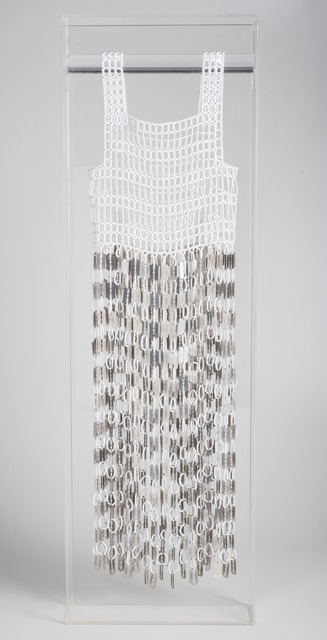
\includegraphics[width=.75\textwidth]{articles/03-contribuicoes-do-sof/image1.pdf}%
        \caption*{Fonte: Acervo da autora (2018).}%
        \label{fig:geogebra-wind}%
    \end{figure}%

    Atualmente, são várias as pesquisas voltadas para investigar as contribuições que o software GeoGebra tem possibilitado tanto no ensino básico como no superior. Entre os pesquisadores podemos citar \textcite{REISAndOZDEMIR2010UsingGeogebra}, \textcite{SHADAANAndEU2013Effec}, \textcite{BORBAAndPENTEADO2007Informática}. Estes defendem que o uso deste software durante as aulas de Matemática permite aos estudantes investigar, experimentar situações, conjecturar, usar sua criatividade além de motivá-los a aprender novos conceitos Matemáticos de forma dinâmica e interativa, de modo que:

    \begin{quotation}
        O software matemático GeoGebra pode beneficiar o processo de ensino e aprendizagem, conduzindo os estudantes por caminhos investigativos. Portanto, consideramos que o computador pode viabilizar a exploração de atividades diversas que podem ser bem enriquecedoras, por oferecer condições as múltiplas representações facilitando as conversões entre essas, onde permite a interatividade entre os objetos matemáticos e a visualização dos conceitos, possibilitando, assim, a formulação de conjecturas \cite[p.~201]{ARAUJOAndSILVA2015GeoGebra}. 
    \end{quotation}

    Além disso, \textcite[p.~571, tradução nossa]{REISAndOZDEMIR2010UsingGeogebra} observam o porquê de usar recursos como o GeoGebra nas aulas de matemática:  

    \begin{quotation}
        A matemática é vista como uma disciplina difícil pelos estudantes durante a vida educacional e seus modelos educacionais são amplamente discutidos (\textit{apud} Altun, 2008). Uma das razões dessas dificuldades são os conceitos abstratos que constituem essa disciplina. A fim de superar essas dificuldades, o uso da visualização ajuda a envolver os alunos, a chamar atenção deles, demonstra como a matemática é relevante para a vida deles e explica como os conceitos matemáticos funcionam (\textit{apud} Murphy, 2009). Desta forma, o resultado das ferramentas da tecnologia da informação no exercício da matemática é contextualizado. 
    \end{quotation}

    Diante das abordagens teóricas até agora apresentadas, o presente trabalho objetiva analisar as contribuições que este software pode trazer para o ensino e aprendizagem de funções, em particular, as Função Polinomial do 2º grau, já que o estudo de funções é um dos temas muito importantes a ser abordado durante o Ensino Médio e que está totalmente relacionado com o cotidiano dos discentes. Além disso, vale salientar que trabalhar este conteúdo apenas utilizando os recursos e métodos convencionais que associam as aulas expositivas com quadro e giz, limita a compreensão de conceitos e a visualização dos objetos Matemáticos. 

    \section{Discussão e métodos}

    Apresentamos nesta sessão uma experiência vivenciada durante as aulas de matemática no Laboratório de Informática da Escola Estadual Edgar Barbosa (Figura \ref{fig:ee-edgar-b}), em específico, nas cinco turmas de 1\textsuperscript{as} séries do Ensino Médio, no qual utilizamos como recurso tecnológico o software GeoGebra para auxiliar nas construções dos gráficos das Funções Polinomiais do 2º grau.

    \begin{figure}[ht]%
        \centering%
        \caption{Escola Estadual Edgar Barbosa}%
        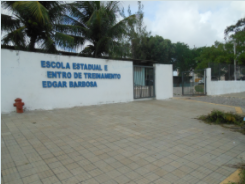
\includegraphics[width=.50\textwidth]{articles/03-contribuicoes-do-sof/image2.png}%
        \caption*{Fonte: Repositório Digital do PIBID.}%
        \label{fig:ee-edgar-b}%
    \end{figure}%

    Atualmente o laboratório de informática da escola (Figura \ref{fig:lab-ee-edgar-b}) é constituído por uma sala climatizada contendo 16 (dezesseis) notebooks, uma bancada de mármore, cadeiras, lousa interativa e um multimídia. Este espaço é frequentemente utilizado pelos professores da escola para ministrar aulas interativas nas áreas de Biologia, Química, Física, Educação Física e Matemática, como também, para que os discentes possam realizar pesquisas.

    \begin{figure}[ht]%
        \centering%
        \caption{Laboratório}%
        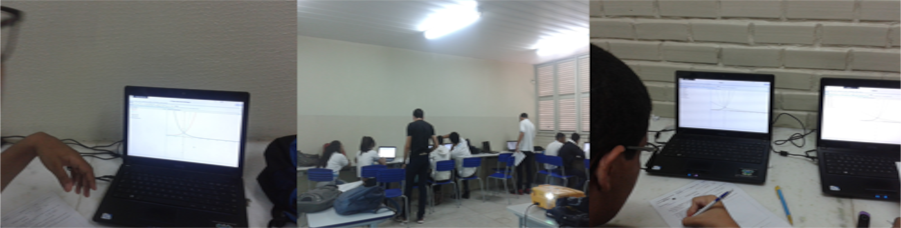
\includegraphics[width=.90\textwidth]{articles/03-contribuicoes-do-sof/image3.png}%
        \caption*{Fonte: Acervo da autora (2018).}%
        \label{fig:lab-ee-edgar-b}%
    \end{figure}%

    Iniciamos, a princípio, apresentando aos discentes o software GeoGebra, que foi utilizado como recurso metodológico para construção de gráficos de funções. Durante este momento, os discentes tiveram a oportunidade de manuseá-lo e conhecer as ferramentas disponíveis no software, para em seguida trabalharmos os gráficos vistos em sala de aula. Portanto, ao iniciarmos nossa pesquisa, usamos como estratégia, as aulas expositivas na sala de aula com construção de gráficos feitos pelos alunos e, em seguida, aulas no laboratório, utilizando as atividades de Função Polinomial do 2º grau. Tomamos como base as atividades propostas no livro didático adotado pela escola, \textcite{DANTE2016Matemática} e \textcite{BALESTRI2016Matemática} porque estes já trazem atividades que já sugerem e orientam o uso do GeoGebra como ferramenta para estudo da construção, comportamento e análise de gráficos. 

    Assim, durante este período foi introduzida a definição de Função Polinomial do 2º grau presente no livro didático: \textit{``Uma função $f: \mathbb{R} \rightarrow \mathbb{R}$ chama-se função quadrática quando existem números reais $a$, $b$ e $c$, com $a \neq 0$, tal que $f$ leva $x$ em {\boldmath$ax^2 + bx + c$}, para todos $x \in \mathbb{R}$.''} \cite[p.~102]{DANTE2016Matemática}.  

    Para familiarizar os discentes com a função, foi apresentado um exercício com várias Funções do 2º grau cuja finalidade era identificar os parâmetros $a$, $b$ e $c$. Em seguida, orientamos e ensinamos aos discentes a fazer o cálculo da imagem da função para os valores atribuídos à variável $x$. Dando continuidade ao estudo, foram abordados os conceitos de raízes da função e pontos de interseção, bem como a resolução de problemas envolvendo Função Polinomial do 2º grau, até darmos início ao estudo dos seus gráficos. 

    Com a desenvoltura do processo, trabalhamos en três momentos distintos a construção dos gráficos da função polinomial. A saber, no primeiro momento introduzirmos gráfico de função por meio das tabelas, isto é, dados os valores da abscissa os discentes determinavam a imagem da função e, em seguida, apresentariam as coordenadas do ponto no plano cartesiano para poderem formar o gráfico da função polinomial do 2º grau. O segundo momento, após termos trabalhado os conceitos de parâmetros, discriminante, ponto máximo e mínimo, vértice do gráfico, concavidade da parábola, passamos a trabalhar com os discentes a construção dos gráficos utilizando estes conceitos. No último momento, com os discentes já familiarizados com as ferramentas do GeoGebra, demos início ao estudo dos gráficos de Função Polinomial do 2º grau, agora com um olhar investigativo. 

    Os três momentos possibilitaram uma investigação da relação entre o pensamento geométrico e algébrico feita pelos discentes. No primeiro momento em que abordados a construção dos gráficos por meio das tabelas, os discentes observaram que os gráficos estavam limitados a quantidade de pontos apresentados e que este processo, dependendo da quantidade de pontos ou do campo de visão do gráfico, limita a visualização do comportamento geométrico da função.  

    Já o segundo momento possibilitou aos discentes visualizarem o comportamento geométrico do gráfico da função de uma maneira mais ampla, já que este procedimento exigiu dos discentes o conhecimento de vários conceitos presentes no estudo do gráfico da Função Polinomial do 2º grau. Entretanto, para a diversidade de comportamentos de gráficos e o curto período de tempo presente na sala de aula ou até mesmo erros algébricos apresentados pelos alunos torna este método limitado. Todavia, a conexão dos métodos empregados nos três momentos tornou o ambiente de aprendizagem enriquecedor, conforme foi observado durante esta investigação em sala de aula. A seguir descrevemos os três momentos e as atividades desenvolvidas com os discentes:
    
    \paragraph{1º momento} Nesta perspectiva, iniciamos nosso percurso apresentando aos discentes algumas Funções Polinomiais do 2º grau e que a partir delas, eles poderiam atribuir valores para abcissa e determinar suas respectivas ordenadas, consequentemente, as coordenadas dos pontos. Posteriormente, teriam o papel de identificar no plano cartesiano os pontos e em seguida traçar o gráfico. A atividade apresentada continha as seguintes funções:
    \begin{itemize}
        \item $f(x) =  x^2 - 7x + 10$
        \item $f(x) =  x^2 - 6x +  9$
        \item $f(x) =  x^2 - 2x +  2$
        \item $f(x) = -x^2 + 2x +  3$
    \end{itemize}
    Cujos respectivos gráficos apresentariam comportamentos conforme observamos nas Figura \ref{fig:graficos-geogebra}:

    \begin{figure}
        \centering%
        \caption{Gráficos das funções}%
        \begin{tabular}{cc}%
            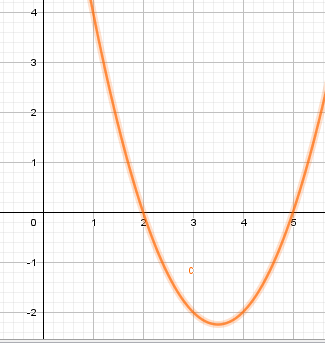
\includegraphics[width=35mm]{articles/03-contribuicoes-do-sof/image4.png}%
            & 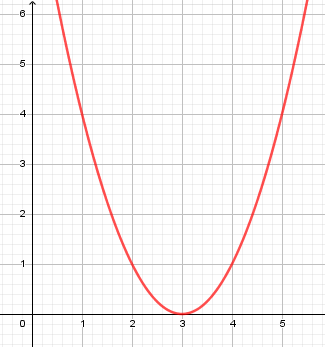
\includegraphics[width=35mm]{articles/03-contribuicoes-do-sof/image5.png}\\%
            (a) $f(x) = x^2 - 7x + 10$ & (b) $f(x) = x^2 - 6x +  9$ \\[2ex]%
            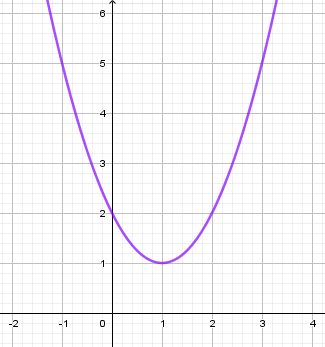
\includegraphics[width=35mm]{articles/03-contribuicoes-do-sof/image6.png}%
            & 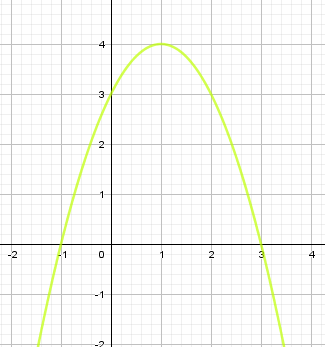
\includegraphics[width=35mm]{articles/03-contribuicoes-do-sof/image7.png}\\%
            (c) $f(x) = x^2 - 2x + 2$ & (d) $f(x) = -x^2 + 2x +  3$ \\%
        \end{tabular}%
        \caption*{Fonte: \textit{Printscreen} dos gráficos no GeoGebra.}%
        \label{fig:graficos-geogebra}%
    \end{figure}

    Estas funções foram escolhidas intencionalmente com aparentes comportamentos distintos, com a finalidade que os discentes fizessem a construção dos gráficos, observando e comparando o comportamento da parábola em cada situação representada. 

    Assim, para a construção dos gráficos, os alunos foram orientados a preencher uma tabela que continha os valores de $x$, mas que deveriam ser calculados os valores da imagem, isto é, $f(x)$. Ao formar as coordenadas dos pontos, eles poderiam traçar o gráfico (fazer a representação gráfica) de cada função dada. Este gráfico era formado por nove pontos, como podemos observar na Figura \ref{fig:atividade}.
    
    \begin{figure}[ht]%
        \centering%
        \caption{Atividade}%
        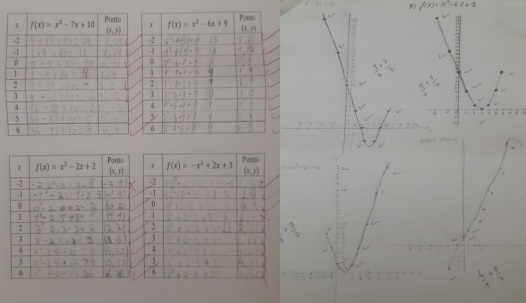
\includegraphics[width=.80\textwidth]{articles/03-contribuicoes-do-sof/image8.jpeg}%
        \caption*{Fonte: Acervo da autora (2018).}%
        \label{fig:atividade}%
    \end{figure}%

    As Figuras \ref{fig:atividade} e \ref{fig:atividade-2} representam os cálculos e a representação gráfica apresentados pelos alunos.

    \begin{figure}[ht]%
        \centering%
        \caption{Atividade}%
        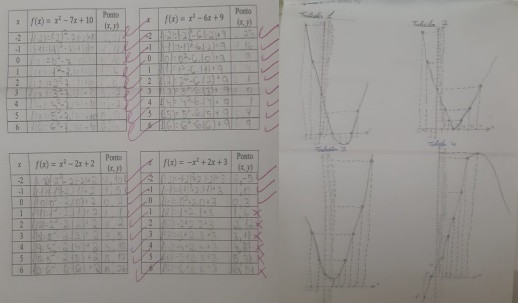
\includegraphics[width=.80\textwidth]{articles/03-contribuicoes-do-sof/image9.jpeg}%
        \caption*{Fonte: Acervo da autora (2018).}%
        \label{fig:atividade-2}%
    \end{figure}%

    Nos cálculos realizados, observamos situações diversas de confusão em relação à identificação das coordenadas, por exemplo, trocavam a ordem do $x$ por $y$, erros cometidos no cálculo da imagem prejudicavam a construção do gráfico, e isso foi notável para construção do gráfico da função $f(x)= -x^2 + 2x + 3$, cuja concavidade da parábola é voltada para baixo, mas a maioria dos alunos esboçaram a concavidade voltada para cima, desconsiderando a regra para o cálculo da potência.

    Ao analisar este primeiro momento, observamos que neste caso o método não traz resultados satisfatórios para o estudo do comportamento do gráfico de uma Função do 2º grau, pois existem erros recorrentes da aritmética resultantes de operações matemáticas quando se há necessidade da análise de sinal, valores da imagem, troca dos valores da abscissa com ordenadas, identificação do ponto no plano cartesiano resultam no erro da construção dos gráficos, pois neste momento supomos que os discentes não tinham conhecimento dos conceitos referentes aos parâmetros, concavidade, vértice e ponto de máximo e mínimo, consequentemente, não possuem a sensibilidade de julgar o gráfico elaborado pelas coordenadas atribuídas por eles. 

    Além disso, o aluno limita a construção dos gráficos apenas aos pontos dados, prejudicando a visualização do comportamento do gráfico, a saber, visualizar vértice, raízes e interseção com eixo $y$. Apesar disso, os discentes argumentam preferir construir os gráficos utilizando tabela, porque acham menos trabalhoso em relação aos cálculos presentes no segundo momento, como veremos a seguir. 

    \paragraph{2º momento} No segundo momento, após apresentarmos aos discentes o gráfico de uma Função Polinomial do 2º grau, trabalhamos com eles os conceitos de parâmetro, raízes da função, os valores do discriminante, eixo de simetria, vértice e valores de máximo e mínimo, propusemos aos alunos atividades que eles pudessem construir os gráficos desta função usando estes conceitos. 

    Desta forma, ao falar de parâmetro, os discentes deveriam estar cientes que o parâmetro $a$ identifica se a concavidade da parábola estará voltada para cima ou para baixo, como também fala sobre a abertura da parábola, o parâmetro $b$ indica se a parábola irá interceptar o eixo $y$ na parte crescente ou decrescente e o parâmetro $c$ expressa o valor em que a parábola irá interceptar o eixo $y$. Em relação ao discriminante, para $\Delta > 0$, a função apresentará duas raízes reais e distintas, ou seja, o gráfico interceptará o eixo $x$ em dois pontos de coordenadas $(x_1, 0)$ e $(x_2, 0)$; para $\Delta = 0$ a função terá duas raízes reais e iguais, ou seja, o gráfico da função intercepta o eixo $x$ em um único ponto; e para $\Delta < 0$, a função não apresenta raízes reais, isto é, o gráfico não irá interceptar o eixo das abscissas. Assim, para construir e analisar o comportamento do gráfico da função do 2º grau, os discentes deveriam ter conhecimento de todos estes conceitos.  

    Quando questionados em relação à atividade anterior, esta, na visão da grande maioria dos discentes é mais trabalhosa, pois requer que os estudantes usem todo embasamento teórico para a construção dos gráficos, conforme foi ensinado na sala de aula. Este embasamento teórico requer que os alunos saibam quando a concavidade da parábola está voltada para cima ou para baixo, se o gráfico da função irá interceptar o eixo da abscissa e em quais valores, os valores de máximo e mínimo da função. Enfim, estes cálculos contribuem para que o gráfico seja visualizado de uma maneira mais detalhada e de forma geral, contribuindo assim, para o sucesso na hora da elaboração dos gráficos. 
    
    Nesta atividade, os alunos identificaram onde o gráfico interceptaria o eixo $x$ e o eixo $y$, se a parábola estava voltada para cima ou para baixo, identificaram o eixo de simetria e os pontos máximo ou mínimo, resultando assim, em uma visão detalhada do comportamento do gráfico. Este método, apesar de ser trabalhoso, possibilita uma compreensão do comportamento do gráfico tornando menores os erros na hora de apresentar o gráfico, além de permitir ao aluno julgar a construção do gráfico por meio dos conceitos apresentados, como pode ser observado nas Figuras \ref{fig:atividade-3} e \ref{fig:atividade-4}.

    \begin{figure}[ht]%
        \centering%
        \caption{Atividade}%
        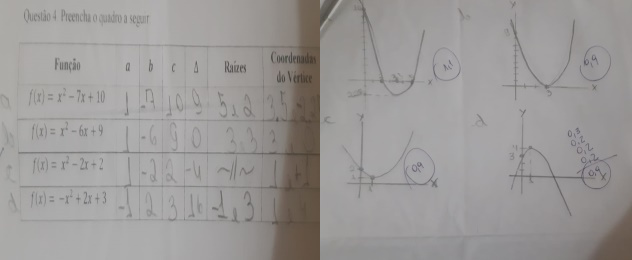
\includegraphics[width=.80\textwidth]{articles/03-contribuicoes-do-sof/image10.jpeg}%
        \caption*{Fonte: Acervo da autora (2018).}%
        \label{fig:atividade-3}%
    \end{figure}%

    \begin{figure}[ht]%
        \centering%
        \caption{Atividade}%
        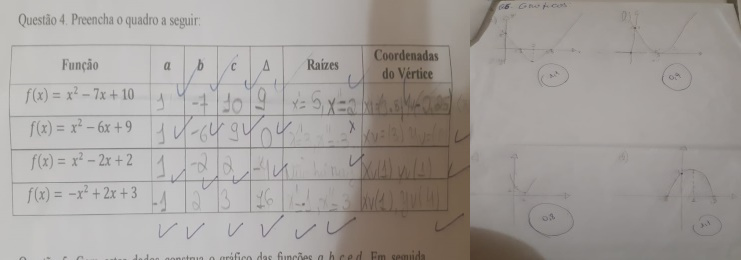
\includegraphics[width=.80\textwidth]{articles/03-contribuicoes-do-sof/image11.jpeg}%
        \caption*{Fonte: Acervo da autora (2018).}%
        \label{fig:atividade-4}%
    \end{figure}%

    Entretanto, apesar destes dois momentos apresentarem sua importância para o ensino e aprendizagem acerca do comportamento dos gráficos, eles requerem tanto do professor quanto dos alunos um maior tempo para que o estudo seja realizado. Há a necessidade da construção de vários gráficos para compreender o papel de cada conteúdo abordado, isto é, para um aluno compreender que o parâmetro $a$ identifica que a concavidade da parábola será voltada para cima ou para baixo, que os valores numéricos deste parâmetro influenciarão na abertura da parábola, necessitasse de atividades que requeiram a construção de vários gráficos para que eles possam assimilar a influência do parâmetro no comportamento do gráfico. 

    Assim, modificando os valores dos parâmetros $a$, $b$ e $c$, observamos que teremos uma determinada função polinomial do 2º grau que corresponderá a um determinado gráfico. Para observarmos o comportamento de diferentes funções há a necessidade de construir diferentes gráficos e analisar a influência do discriminante, dos valores dos parâmetros e raízes. Todavia, há um programa a ser seguido durante todo o ano letivo, assim, os docentes acabam limitando as variedades de exemplos que poderiam ser apresentados, tornando o trabalho do professor limitado a apresentar poucas funções. 

    Em oposição aos métodos de ensino expositivo, a saber, aqueles em que o professor e os discentes ficam limitados ao: quadro, projetores multimídia, aos livros e atividades didáticas; softwares como o GeoGebra abrangem novas possibilidades de ensino e aprendizagem, já que este ambiente interativo favorece o trabalho do professor na hora de ministrar os conteúdos relacionados a gráficos de função e possibilita a construção, a análise do comportamento dos gráficos e a compreensão dos conceitos abordados em sala de aula. 

    \paragraph{3º momento} O terceiro momento foi caracterizado por trabalharmos com os alunos a construção dos gráficos da Função Polinomial do 2º grau por meio do software GeoGebra. Inicialmente, os alunos conheceram o laboratório de informática da escola (Figura \ref{fig:atividade-5}) onde apresentamos o software, sua barra de ferramentas, comandos de entrada, as janelas algébrica, geométrica e os comandos que usaríamos para o estudo das funções. Assim, esta aula ficou voltada para que os discentes conhecessem e manipulassem as ferramentas do software GeoGebra.

    \begin{figure}[ht]%
        \centering%
        \caption{Atividade}%
        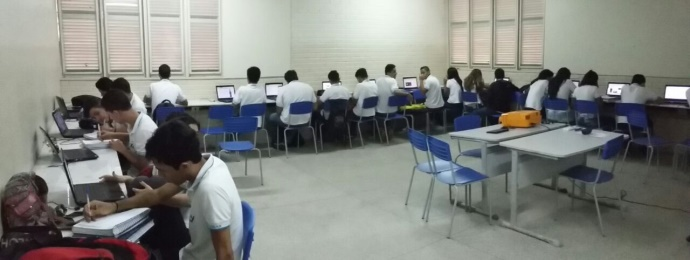
\includegraphics[width=.80\textwidth]{articles/03-contribuicoes-do-sof/image12.jpeg}%
        \caption*{Fonte: Acervo da autora (2018).}%
        \label{fig:atividade-5}%
    \end{figure}%

    Finalizada esta etapa, aplicamos atividades que abordavam a construção de gráficos usando o software GeoGebra. Iniciamos por uma atividade em que os alunos, utilizando o comando de entrada, digitavam a expressão algébrica da Função Polinomial do 2º grau e o software apresentava o desenho da parábola na janela geométrica, apresentava as raízes, o ponto de interseção com eixo y e o ponto que representava o vértice da parábola. Além disso, estes dados poderiam ser conferidos pelos discentes na janela algébrica. Feito isto, os discentes manualmente conferiram os dados apresentados pelo software utilizando os conceitos estudados em sala de aula (Figura \ref{fig:atividade-6}). 

    \begin{figure}[ht]%
        \centering%
        \caption{Atividade}%
        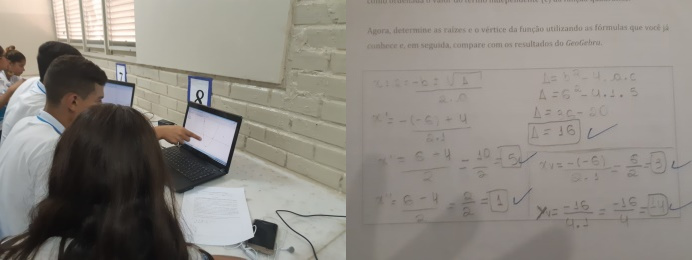
\includegraphics[width=.80\textwidth]{articles/03-contribuicoes-do-sof/image13.jpeg}%
        \caption*{Fonte: Acervo da autora (2018).}%
        \label{fig:atividade-6}%
    \end{figure}%

    A segunda atividade usando o GeoGebra (Figura \ref{fig:atividade-7}) constituía-sa em uma sequência de passos a ser realizada no software. Neste momento, foi utilizado o comando controle deslizante (ferramenta do GeoGebra que permite inserir uma variável que pode ser alterada utilizando o mouse) para representar os parâmetros $a$, $b$ e $c$ na função $f(x) = ax^2 + bx + c$ e que possibilitou aos discentes manipulá-los de tal forma que poderiam visualizar os efeitos dos valores dos parâmetros sobre o gráfico da função.

    \begin{figure}[ht]%
        \centering%
        \caption{Atividade}%
        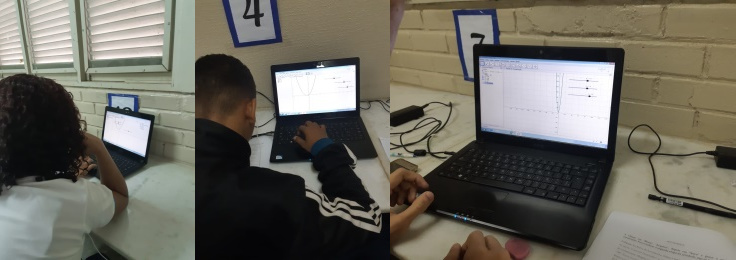
\includegraphics[width=.80\textwidth]{articles/03-contribuicoes-do-sof/image14.jpeg}%
        \caption*{Fonte: Acervo da autora (2018).}%
        \label{fig:atividade-7}%
    \end{figure}%

    Este momento possibilitou aos discentes, em um curto período de tempo, uma maior variedade de gráficos, contribuiu para que eles compreendessem os conceitos apresentados em sala de aula, como por exemplo, que a abertura e sentido da concavidade de uma parábola dependem dos valores do parâmetro $a$, que a interseção da parábola no eixo $y$ será no ramo crescente se valor do parâmetro $b$ for positivo e será no ramo decrescente se o valor de $b$ for negativo, e o parâmetro $c$ corresponde ao valor em que a parábola intersecta o eixo $y$. Possibilitou a visualização de gráficos no centro do eixo do plano cartesiano e também gráficos distantes deste eixo, permitindo visualizar pontos de intersecção, vértice e concavidade, além de identificar domínio e imagem deste tipo de função. 

    Enfim, as aulas ministradas no laboratório utilizando como recurso metodológico o software GeoGebra possibilitaram, tanto ao professor como aos discentes, várias oportunidades, pois usando este ambiente interativo, os discentes puderam fazer o estudo dos gráficos de forma dinâmica, possibilitando assim, plotar os gráficos de diferentes funções em um mesmo ambiente interativo, comparar e analisar o comportamento dos diversos gráficos em curto período de tempo. Desta forma, o uso deste software torna o ambiente de sala de aula motivador e enriquecedor. 

    Assim, ao solicitarmos para que os alunos descrevessem a importância do uso do software GeoGebra para o ensino aprendizagem da Matemática, destacamos três respostas entre tantas outras similares:
    \begin{quotation}
        \medskip\noindent{}Aluno A: “Utilizar mais o uso do GeoGebra, na minha opinião facilita para quem tem um baixo desenvolvimento em desenvolver um gráfico (tipos eu)\dots~Podemos utilizar da melhor forma e adquirir um nível de aprendizado.”

        \medskip\noindent{}Aluno B: “Eu acho que devemos continuar as aulas no laboratório com o GeoGebra, porque esse programa permite a criação de atividades que exploram diversos conteúdos matemáticos de maneira prática, instigante, dinâmica e eficiente no nosso aprendizado.” 
        
        \medskip\noindent{}Aluno C: “Eu acho que o uso do GeoGebra ajuda na parte da interpretação de um gráfico, já que muitos não conseguem fazê-los perfeitamente. Com o uso do aplicativo podemos assim trazer e resolver nossas dúvidas os gráficos onde não conseguimos representar.” 
    \end{quotation}
    Estas falas foram extraídas de uma enquete feita no grupo do WhatsApp da turma, conforme representadas na Figura \ref{fig:relatos-wpp}.

    \begin{figure}[ht]%
        \centering%
        \caption{Relatos do grupo do WhatsApp}%
        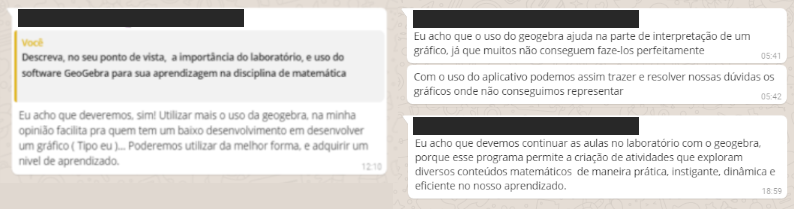
\includegraphics[width=.90\textwidth]{articles/03-contribuicoes-do-sof/image15.png}%
        \caption*{Fonte: Acervo da autora (2018).}%
        \label{fig:relatos-wpp}%
    \end{figure}%

    Entretanto, vale salientar que, assim como nos momentos anteriores, o uso desta ferramenta possui suas limitações, pontos negativos. Entre estes pontos, temos a própria estrutura do laboratório, pois são poucos os computadores para a quantidade de alunos por turma. Apesar de vivermos num ambiente em que a tecnologia se faz presente, ainda encontramos discentes que possuem dificuldades em manusear um computador. Em relação ao software, alguns estudantes argumentaram não saber manipular o GeoGebra e ter que ficar sempre pedindo ajuda da professora. Mas, tais limitações não superam a importância que este recurso traz para o ensino e aprendizagem de funções, pois manipular, visualizar, comparar e investigar possibilita o desenvolvimento de habilidades ao aluno tais como: a curiosidade, sensibilidade e autonomia.

    \section{Considerações finais}

    Aprender é um processo árduo que requer do sujeito interesse, força de vontade, motivação e curiosidade. Porém, nem sempre escolhemos aprender o que desejamos, mas somos levados a conhecer o que é necessário para nos tornarmos cidadãos críticos e conhecedores do mundo em que vivemos. Assim, nem tudo que aprendemos é porque queremos, mas porque se faz necessário. 

    Desta forma, a escola possui o papel de mediar o conhecimento gerado pela humanidade e os valores aplicados na sociedade. Isso provoca um choque no sujeito que está aprendendo, que se questiona: “onde usarei isto na minha vida?”. Que importância terá para este sujeito aprender a construir ou interpretar um gráfico? Como um professor de matemática poderá motivar estes discentes tornando sua aula mais atrativa? O mais importante ainda é: Como levá-lo a compreender, de forma significativa, aquilo que se é ensinado? São questões que são frequentemente levantadas pelos educadores e sujeitos da aprendizagem. 

    Foi com a intenção de motivar a aprendizagem de forma significativa que este trabalho analisou as contribuições que o software GeoGebra poderia trazer para o ensino e aprendizagem de funções do 2º grau por meio de atividades realizadas no laboratório da escola e na sala de aula. Assim, para atribuirmos a importância deste recurso metodológico para a sala de aula, optamos por trabalhar com os discentes três modos para o estudo do gráfico da função polinomial do 2º grau, a fim de compararmos os processos apresentados e acompanhar a desenvoltura dos alunos em relação a cada momento. 

    Compreendemos que cada momento teve sua importância, mas também as limitações no ensino-aprendizagem de funções polinomiais do 2º grau. Porém, o uso de recurso metodológico, como o software GeoGebra contribui de forma significativa para entender os conceitos relacionados à construção dos gráficos de uma função, em particular, as funções polinomiais do 2º grau. Isto porque o ambiente interativo do software possibilita verificar diferentes gráficos em mesmo sistema de eixo, o comportamento da função em relação aos seus parâmetros, identificar os conceitos de função abordados em sala de aula, além de, simplificar o tempo de abordagem do conteúdo. As aulas tornam-se atrativas, despertando nos discentes, a curiosidade, senso investigativo e desejo em aprender. 

    O uso deste recurso, em comparação com os momentos anteriores, foi bem-visto pelos discentes que argumentaram estar mais instigados, possibilitando aprender matemática de uma forma diferente, a tecnologia foi usada para algo produtivo, os discentes puderam interagir entre si por ser algo novo e diferente. Contribuiu para que a professora apresentasse o conteúdo de uma forma interativa inovadora. 

    Enfim, apesar das limitações detectadas durante o uso do GeoGebra nas atividades propostas, avaliamos que foi de fundamental importância compreender as estruturas das funções e observar que cada função possui um gráfico, suas características e comportamento que ficam mais interessantes de serem estudadas em um ambiente interativo. 

    \printbibliography[heading=subbibliography,notcategory=fullcited]

    \nocite{DocumentoInstitucional2006Orientações}
    \nocite{DocumentoInstitucional2017Escola}

    \label{chap:contrib-geogebraend}

\end{refsection}

\begin{refsection}
    \renewcommand{\thefigure}{\arabic{figure}}
    
    \chapterTwoLines
    {Matemática na arte}
    {Uma proposta interdisciplinar para o ensino de geometria}
    \label{chap:matematicanaarte}
    
    \articleAuthor
    {Charles Ricardo Lemos de Melo}
    {Graduado em Matemática pela Universidade Federal do Rio Grande do Norte (UFRN). Graduação em Engenharia Civil pela UFRN. Especialista em Avaliação e Perícia de Engenharia pelo Centro de Pós-Graduação, Pesquisa e Difusão Cultural das faculdades Oswaldo Cruz. Professor da rede estadual do RN. E-mail: charlesrlemos@hotmail.com.}
    
    \articleAuthor
    {Wguineuma Pereira Avelino Cardoso}
    {Graduada em Matemática pela Universidade Federal do Rio Grande do Norte (UFRN). Graduação em Pedagogia pela UFRN. Especialização na área da Matemática para o Ensino Fundamental e Ensino Médio pelo Instituto Superior de Educação Presidente Kennedy. Mestrado na área de Ensino e Ciências pela UFRN. Doutoranda em Ensino de Ciências e Matemática pelo PPGECM (UFRN). ID Lattes: 3384.1278.8608.5225. ORCID: 0000-0002-5587-5766. E-mail: wguineuma@ifesp.edu.br.}
    
    \begin{galoResumo}
        \marginpar{
            \begin{flushleft}
            \tiny \sffamily
            Como referenciar?\\\fullcite{SelfMeloAndCardoso2021Matemática}\mybibexclude{SelfMeloAndCardoso2021Matemática}, p. \pageref{chap:matematicanaarte}--\pageref{chap:matematicanaarteend}, \journalPubDate{}
            \end{flushleft}
        }
        Este artigo aborda uma pesquisa que teve como objetivo investigar como a Arte pode contribuir no ensino e aprendizagem da Geometria. Elaboramos uma proposta interdisciplinar de ensino que utiliza imagens de telas de pintura a óleo como veículo de investigação dos elementos geométricos presentes nestas. Utilizamos telas de autoria do professor investigador da pesquisa e algumas composições dos artistas Mondrian e Kandinsky. A pesquisa experimental foi desenvolvida em uma escola pública, com alunos do 6º ano do Ensino Fundamental. Verificamos uma maior participação por parte dos alunos em sala e, ainda, uma atitude mais reflexiva e significativa, durante as discussões referentes aos conteúdos geométricos. 
    \end{galoResumo}
    
    \galoPalavrasChave{Artes Visuais. Formas Geométricas. Ensino.}
    
    \begin{otherlanguage}{english}
    
    \fakeChapterTwoLines
    {Mathematics in art}
    {An interdisciplinary proposal for geometry teaching}
    
    \begin{galoResumo}[Abstract]
        This article addresses a research that aimed to investigate how Art can contribute to the teaching and learning of Geometry. We developed an interdisciplinary teaching proposal that uses images from oil painting canvases as a vehicle for investigating the geometric elements present in them. We used canvases authored by the research professor and some compositions by artists Mondrian and Kandinsky. The experimental research was carried out in a public school, with students from the 6th year of elementary school. We verified a greater participation by the students in the classroom and, also, a more reflective and significant attitude during the discussions regarding geometric contents. 
    \end{galoResumo}
    
    \galoPalavrasChave[Keywords]{Visual arts. Geometric shapes. Teaching.}
    \end{otherlanguage}

    \section{Introdução}

    O ser humano está inserido em um mundo cercado de formas, sejam elas regulares ou irregulares, e é na Geometria que está organizada o conhecimento para entender esse espaço físico cercado de modelos geométricos no qual vivemos. Por isso, nos motivamos como docente, a tentar estimular o aluno a apropriar-se dos conhecimentos advindos da Geometria de modo a propiciar o seu desenvolvimento cognitivo na área da Matemática além de contribuir para obtenção de uma efetiva relação dessa área do conhecimento com o mundo que o cerca. 

    Em nossa prática docente, na disciplina de Matemática, com estudantes do Ensino Fundamental e do Ensino Médio, pudemos observar por diversas vezes, que os alunos podem apresentar algumas dificuldades em aprender Geometria. E essas dificuldades muitas vezes advêm de dois fatores: O primeiro é que uma boa parte dos professores privam os alunos da aprendizagem de Geometria, na medida em que selecionam os conteúdos que serão estudados em sala de aula. O outro fator a ser considerado, diz respeito a forma que alguns discentes ministram os conceitos geométricos em sala. Sobre isso alguns autores enfatizam que: 

    \begin{quotation}
        Os conceitos são ideias a serem construídas pelo aluno. Esta construção exige o trabalho de mediadores (professores, colegas materiais instrucionais, entre outros) que contribuam para atribuições de significado aos fenômenos estudados, no caso associados às formas, ao espaço ou suas representações. \cite[p.~7]{RÊGOAndRÊGOAndKLEBER2012Laboratório}.
    \end{quotation}

    Assim, é necessário que os conteúdos geométricos sejam apresentados de uma forma mais significativa para os estudantes, uma sugestão seria associar a Geometria a outras áreas de conhecimento. 

    Utilizando como pressuposto que o ensino da Matemática tenha uma relevância considerável para o processo de formação social e cultural dos indivíduos, a presente pesquisa tem como intuito buscar outras formas de ensino e aprendizagem da Matemática aliada a outras áreas do conhecimento, de modo que seja proporcionado aos alunos um aprendizado que o estimule a raciocinar sobre a Geometria presente no seu cotidiano.  

    Diante disso, temos vários questionamentos vivenciados em nossa prática: De que forma poderíamos associar a Matemática do cotidiano aos nossos alunos? O que fazer para apresentar o conteúdo de Geometria, em especial, o estudo das principais figuras planas de uma forma prazerosa, amena e interessante, sem que se perdesse de vista o seu rigor, no que diz respeito aos conceitos matemáticos? Como utilizar outras áreas do conhecimento no ensino de Matemática? 

    A partir do que foi posto, propomos agregar o ensino da Geometria, no que diz respeito aos conceitos de figuras planas, à Arte e, no caso particular a pintura, tentando integrá-los, de um modo harmonioso e atrativo para os discentes, além de oportunizar a inserção de elementos artísticos ao longo do processo, propiciando uma conexão da disciplina de Matemática com a Arte, em especial às Artes Visuais, de modo a contribuir para uma efetiva apropriação, pelos alunos, dos conceitos geométricos apresentados em sala, além de tornar as aulas de Geometria mais dinâmicas imbricadas de significados. 

    Assim, nosso objetivo é investigar como a Arte pode contribuir no processo ensino-aprendizagem da Geometria em duas turmas do 6º Ano do Ensino Fundamental. Além disso, buscamos identificar as potencialidades e limitações no ensino de Geometria aliado à Arte; elaboramos e aplicamos algumas atividades didáticas, e por fim planejamos e desenvolvemos aulas, em uma escola pública do Rio grande do Norte (RN), nas quais utilizamos a Arte como caminho para o ensino e aprendizagem de Geometria. E, uma de nossas referências para essa investigação foi à interdisciplinaridade de \textcite{FAZENDA2011Integração}, que tem como princípio reconhecer as limitações nas aprendizagens fragmentadas \cite{FAZENDA2011Integração}. E depois, por meio dos experimentos e das atividades realizadas, fizemos nossas observações de campo, que segundo, \textcite{LAVILLEAndDIONES1999Construção}:  

    \begin{quotation}
        [\dots] revela-se certamente nosso privilegiado modo de contato com o real: e observando que nos situamos, orientamos nossos deslocamentos, reconhecemos as pessoas, emitimos juízos sobre elas. Sem alongar inutilmente essa lista, convenhamos que, em nossas atividades quotidianas, não há quase exemplos que não deixem espaço a observação \textcite[p.~177]{LAVILLEAndDIONES1999Construção}. 
    \end{quotation}

    Dessa forma, a observação das experiências desenvolvidas em campo, permitiu um olhar para nosso objeto de pesquisa. Assim, descrevemos nossas observações neste artigo que está dividido em quatro partes, na primeira, temos uma breve introdução apontando a importância e as dificuldades no ensino de Geometria como também nosso objetivo de pesquisa. A segunda é composta por uma discussão sobre a interdisciplinaridade, que foi nosso principal referencial teórico, e as conexões entre a Arte e a Matemática e na terceira, colocamos nossa abordagem metodológica de pesquisa e os caminhos que tomamos para realizar a atividade de campo. Por último, as considerações finais, que apontam os resultados da pesquisa e nossas conclusões.

    \section{A interdisciplinaridade no ensino da matemática: a arte como aliada no estudo da geometria}

    A prática da interdisciplinaridade na Educação não deve ser vista de um modo simplista e utilizada pelo professor apenas como uma forma de integração entre áreas do conhecimento. Uma atitude interdisciplinar do docente exige, antes de tudo, que a sua prática cotidiana seja por ele amplamente investigada. Segundo, \cite{FAZENDA2011Integração}, é importante buscar uma integração de conhecimentos de modo eficiente, com o objetivo de proporcionar questionamentos nos quais propicie a transformação da realidade. Ela ainda nos diz que a: 

    \begin{quotation}
        [\dots] integração em relação à interdisciplinaridade, conclui-se em favor da necessidade da integração como momento, como possibilidade de atingir uma “interação”, uma interdisciplinaridade com vistas a novos questionamentos, novas buscas, enfim, para uma mudança na atitude de compreender e entender \cite[p.~84]{FAZENDA2011Integração}.
    \end{quotation}

    Essa mudança de atitude se inicia pelo professor, que ao perceber o desinteresse do aluno em aulas dadas de forma tradicional, dogmática e sem sentido, procura novos caminhos metodológicos. Professores em sua prática docente sentem bastante dificuldades em ministrar os conteúdos geométricos de uma forma contextualizada. A interdisciplinaridade pode ser uma forma de construir os saberes e superar os diversos problemas vivenciados no processo ensino e aprendizagem da Matemática, em especial da Geometria, tornando o ensino prazeroso e a aprendizagem mais interessante para os alunos. 

    Evidenciando a importância da interdisciplinaridade, \textcite{ALVES2008Interdisciplinaridade} afirma: 

    \begin{quotation}
        Assim, vemos a interdisciplinaridade como uma "nova" atitude frente ao conhecimento, na busca do sentido do saber, procurando superar a insatisfação que a fragmentação cria. Ainda que seja uma busca utópica da totalidade, é o desejo de um ensino que considere a emoção tanto quanto a razão. \cite[p.~100]{ALVES2008Interdisciplinaridade}.
    \end{quotation}


    Destacando também a inter-relação entre a Matemática e Arte, \textcite{ALBUQUERQUE2017Geometria} declara: 

    \begin{quotation}
        Assim, a matemática e a arte, em suas diversas expressões, guardam uma relação muito próxima, quer seja na arquitetura de Oscar Niemeyer, quer seja nas telas de Tarsila do Amaral, nas construções de Leonardo Da Vinci, nas simetrias de M. C. Escher, no artesanato dos filés alagoanos, nos desenhos estampados nas cerâmicas indígenas, para onde olhamos vemos essa proximidade. A beleza com a qual as duas dialogam é enorme. \cite[p.~46]{ALBUQUERQUE2017Geometria}.
    \end{quotation}

    O papel do professor é procurar desvendar meios viáveis de apresentar os conteúdos de modo que propicie aos seus alunos uma efetiva apropriação das informações e, assim, os tornem plenamente capazes de formar o conhecimento necessário para suas interações com o mundo real.  

    Temos o sentimento de que o ensino da Geometria demanda a utilização de uma diferenciada prática pedagógica, uma vez que este conhecimento da Matemática propicia a integração dos conceitos geométricos a um trabalho mais concreto e dinâmico. Os métodos de ensino precisam oportunizar os alunos a perceberem a Geometria como uma ferramenta útil no relacionamento de cada indivíduo com o mundo. \textcite{CONTIEROAndGRAVINA2011Modelagem} fazem alusão a uma forma equivocada de apresentação dos conteúdos da Geometria nos livros didáticos cuja essência está na repetição de conceitos e propriedades em detrimento de se desenvolver aspectos cognitivos dos alunos, em especial, a capacidade de abstração.  

    \begin{quotation}
        O estudo da Geometria escolar tem foco na apresentação de conceitos e propriedades geométricas, sem que haja maiores preocupações com o desenvolvimento do raciocínio geométrico. Os livros apresentam uma coleção de definições e as propriedades são tomadas como “fatos”, sem que haja uma maior explicação \cite[p.~2]{CONTIEROAndGRAVINA2011Modelagem}.
    \end{quotation}

    Percebe-se que a metodologia na qual a Geometria vem sendo trabalhada no ensino da Educação Básica, acaba não permitindo que os alunos desenvolvam, satisfatoriamente, a habilidade de construção de novos conceitos matemáticos, dificultando, assim, a promoção de uma aprendizagem significativa.  

    Destacamos também, sobre a interdisciplinaridade, a declaração presente nos Parâmetros Curriculares Nacionais do Ensino Médio (PCNEM), afirmando que: 

    \begin{quotation}
        A interdisciplinaridade também está envolvida quando os sujeitos que conhecem, ensinam e aprendem sentem necessidade de procedimentos que, numa única visão disciplinar, podem parecer heterodoxos, mas fazem sentido quando chamados a dar conta de temas complexos. Se alguns procedimentos artísticos podem parecer profecias na perspectiva científica, também é verdade que a foto do cogumelo resultante da explosão nuclear também explica, de um modo diferente da Física, o significado da bomba atômica. \cite[p.~75]{ParâmetrosCurricularesMatematica2000}. 
    \end{quotation}

    \textcite{PEREIRA2016Arte} destaca o fato de que, apesar de parecer abstrato uma integração entre a Arte e Geometria, há diversos exemplos do uso de conceitos geométricos por muitos profissionais das artes quando do desenvolvimento de suas formas de expressão visual. 

    \begin{quotation}
        Associar Arte e Geometria pode parecer um tanto abstrato e sem uma referência concreta. Contudo, a própria história da humanidade apresenta diversos momentos em que artistas se utilizaram da Geometria para expressar-se artisticamente. \cite[p.~28]{PEREIRA2016Arte}. 
    \end{quotation}

    E ainda seguindo nesta linha de pensamento, consta nos Parâmetros Curriculares Nacionais:

    \begin{quotation}
        [\dots] É fundamental que os estudos do espaço e forma sejam explorados a partir de objetos do mundo físico, de obras de arte, pinturas, desenhos, esculturas e artesanato, de modo que permita ao aluno estabelecer conexões entre a Matemática e outras áreas do conhecimento. \cite[p.~51]{ParâmetrosCurricularesMatematica1998}.
    \end{quotation}

    Temos o entendimento de que a utilização das ideias referidas acima pode favorecer uma abordagem bastante ``fértil'' nas práticas pedagógicas nos diversos níveis de ensino, além de proporcionar meios pelos quais se conquiste a superação do aspecto fragmentado de produção do conhecimento geométrico, em que são realizados cálculos a partir das propriedades apresentadas em sala de aula, sem que se faça o uso de abstrações, como também, sem oportunizar a prática da utilização do manuseio de objetos presentes na vida cotidiana dos aprendizes. 

    \textcite{LAURO2008Discutindo}, ressaltando a importância da Geometria para o homem no seu cotidiano, afirma que:

    \begin{quotation}
        Os objetos do mundo físico possuem alguma forma e tamanho ou ocupam alguma posição no espaço. Assim, as formas ou padrões geométricos constituem os modelos mais elementares para muitos tipos de fenômenos da nossa vida cotidiana, tais como medir (as dimensões de um apartamento); examinar formas (a forma de um favo de mel, das moléculas de um cristal, das células, de algumas conchas do mar ou das pétalas de uma flor), comparar tamanhos (a água deste copo cabe naquela xícara?), analisar posições (A rua A é perpendicular ou paralela à rua B), representar e construir (a planta e a maquete de uma casa). A geometria é a ferramenta que o ser humano criou para estudar essas entre outras questões. \cite[p.~178]{LAURO2008Discutindo}.
    \end{quotation}

    \textcite{PEREIRA2016Arte} comenta a respeito da importância do uso da intuição tanto para aquele que exercita a Arte quanto para quem trabalha com a Matemática. 

    \begin{quotation}
        Quando um artista exercita a imaginação, ele realiza combinações de imagens, visualiza e representa o mundo. Para isto, necessita compreender o espaço e a forma das coisas que o rodeiam. Na Arte e na Matemática, o uso da intuição sempre foi imprescindível para a realização de descobertas. Ambos, Matemática e Arte, apresentam em suas especificidades contribuições: uma a beleza estética da representação, a outra a beleza estética do raciocínio. \cite[p.~33--34]{PEREIRA2016Arte}.
    \end{quotation}

    A Geometria na Arte pode ser facilmente constatada em diversos trabalhos artísticos, especialmente na pintura, em que verificamos elementos geométricos dos mais variados tamanhos e formas em muitas obras de pintores reconhecidos.  

    Podemos citar alguns artistas, das Artes Plásticas que suas obras retratam imagens geométricas, e estas podem ser usadas como exemplos do uso criativo e harmonioso dessa interação entre as duas áreas do conhecimento, as Artes e a Matemática, entre eles identificamos Piet Mondrian, Wassily Kandinsky, Paul Klee e Mourits Escher. \cite{WIKIARTEnciclopédia}.

    Todos eles realizaram composições artísticas onde a presença de elementos geométricos interagindo com cores e formas é facilmente percebida pelo eventual observador. Este fato evidencia certo grau de conhecimento de Geometria por parte desses artistas, ainda que em certos casos isso fosse um tanto quanto intuitivo. É relevante destacar que tais pintores foram capazes de utilizar esses saberes como suporte para elaboração de trabalhos artísticos que personificaram o pensar interdisciplinar de cada um deles.  

    Apontando algumas possibilidades da utilização de elementos matemáticos como forma de expressão da Arte e que foram usados por artistas como Kandinsky, Mondrian e Klee, apresentamos a seguinte declaração de \textcite{ARAÚJO2008Ponto}: 

    \begin{quotation}
        Para estabelecer a convergência nos ensinos dessas duas áreas de conhecimento destaca-se o Movimento Modernista e com ele os pintores Kandinsky (1925), Mondrian (1937), Klee (1979), que expressaram a linguagem da arte por meio de elementos matemáticos \cite[p.~61]{ARAÚJO2008Ponto}. 
    \end{quotation}

    Focando as atenções no ensino da Geometria e repensando nossa prática pedagógica objetivando a conquista de novas ações que viabilizem a criação de novas situações que promovam uma efetiva aprendizagem, realizamos esta pesquisa que se orienta pelo desejo de criar um ambiente de sala de aula no qual a Geometria esteja associada à Arte.  

    Nesse sentido, construímos uma proposta de trabalho favorável à aprendizagem dos alunos e que contribua para potencializar a apropriação de conceitos geométricos referentes ao estudo das principais figuras planas, além de viabilizar o surgimento de um ambiente rico e motivador, o qual seja capaz de frutificar diálogos e descobertas que possam levar os alunos a transcenderem o formalismo da apresentação dos conteúdos matemáticos, como também impulsionar a capacidade de construção de um conhecimento em que, a intuição, o senso crítico, a percepção e a imaginação se façam plenamente presentes e favoreçam a integração dos saberes matemáticos com os demais conhecimentos.  

    Portanto, fizemos e aplicamos uma proposta didática com a Geometria aliada à Arte, e utilizamos composições de artistas renomados como também de telas produzidas pelo próprio pesquisador. Assim, foram trabalhados os conceitos e propriedades das principais figuras planas, promovendo discussões a respeito de como a Matemática favoreceu no processo da criação artística de muitos daqueles considerados como grandes nomes das artes. 

    \section{Sistematização do percurso}

    Esta pesquisa foi realizada em uma abordagem qualitativa de pesquisa, na qual se buscou a obtenção de dados descritivos em campo pelo pesquisador. Segundo \textcite{BOGDANAndBIKLEN1994Investigação}, a investigação qualitativa deve atender algumas características, entre elas, a investigação é descritiva, pois os dados recolhidos serão apresentados sob a forma de palavras, não utilizando base numérica; O foco da pesquisa será o processo, ou seja, como e por que as coisas acontecem; Os dados foram analisados de forma indutiva, ou seja, construídas a partir do exame de cada atividade realizada, tendo interesse no significado das visões de mundo de cada participante do processo a fim de se verificar como eles as interpretam \cite{BOGDANAndBIKLEN1994Investigação}. 

    Assim, para analisar os procedimentos da pesquisa fizemos estudos bibliográficos sobre a interdisciplinaridade no Ensino da Matemática. À integração e interdisciplinaridade no ensino brasileiro; o uso da Arte aliada ao ensino de Matemática. Sendo nossos referenciais, \textcite{FAZENDA2011Integração} e \textcite{ARAÚJO2008Ponto}, entre outros. 

    Iniciamos com a composição de sete quadros\footnote{Os sete quadros são uma criação do autor da pesquisa.}, sendo que em seis deles utilizamos a técnica em “óleo sobre tela” (utiliza tinta a óleo e pincel) e um executado com lápis de cor. Intitulamos todas as telas de “figuras planas”, conforme estão retratadas na Figura \ref{fig:figuras-planas}. As sete composições foram idealizadas e estruturadas sob a perspectiva de contextualizar as aulas de Geometria com a Arte de uma forma integrada, oportunizando aos alunos momentos de discussão sobre a importância do conhecimento geométrico, ainda que de forma superficial, no cotidiano de diversos tipos de profissionais, especialmente aqueles que lidam com artes visuais, bem como na vida diária de um cidadão comum e, também, apresentar a Matemática como uma possível aliada das várias áreas do conhecimento. 

    \begin{figure}[ht]%
        \centering%
        \caption{Figuras planas}%
        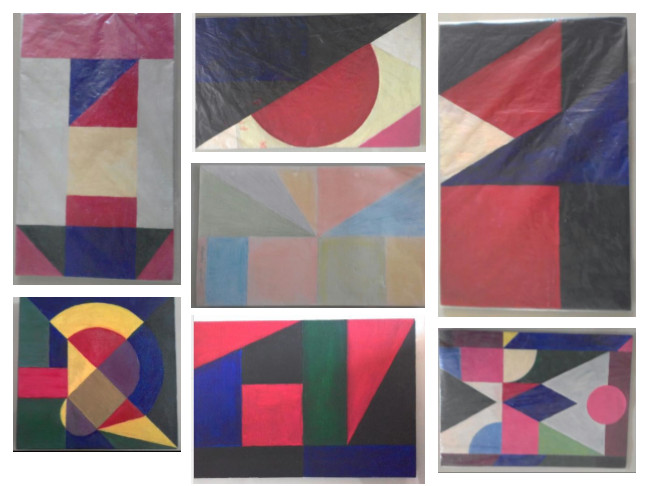
\includegraphics[width=.5\textwidth]{articles/04-matematica-na-arte--/figura1.jpg}%
        \caption*{Fonte: Elaborado pelo autor.}%
        \label{fig:figuras-planas}%
    \end{figure}%

    Vale ressaltar também que esta pesquisa foi realizada em uma Escola Pública da Rede Estadual do RN, em oito encontros vivenciais com duas turmas do 6º ano do Ensino Fundamental. Para esses encontros chamamos de “momentos”. Durante os encontros utilizamos como instrumento de coleta de dados, o diário de campo, para anotar nossas observações e as atividades práticas realizadas pelos alunos. A descrição de cada um desses “momentos” foi realizada em ordem cronológica para proporcionar uma melhor visão da pesquisa.  

    No primeiro momento apresentamos fotografias ampliadas de pinturas de autoria dos artistas Mondrian e Kandinsky conhecidos internacionalmente por utilizarem, em diversas de suas composições, elementos geométricos das mais variadas formas, conforme apresentadas nas Figuras \ref{fig:composicaoII}, \ref{fig:composition-a}, \ref{fig:arch-and-point} e \ref{fig:arch-and-point}. O nosso intuito foi tentar instigar o interesse dos alunos pelas figuras geométricas identificadas nas obras e, a partir de então, iniciar uma primeira discussão sobre como a Matemática interage com outras áreas do conhecimento, especialmente com a Arte. Neste momento discorremos sobre os conceitos elementares da Geometria, sobre figuras planas e suas principais propriedades. Percebemos que os estudantes tinham dificuldades em distinguir o círculo da circunferência, como também, em relação à ideia de raio e diâmetro. 

    \begin{figure}[ht]%
        \centering%
        \caption{Piet Mondrian, \textit{Composição II em Vermelho, Azul e Amarelo.}}%
        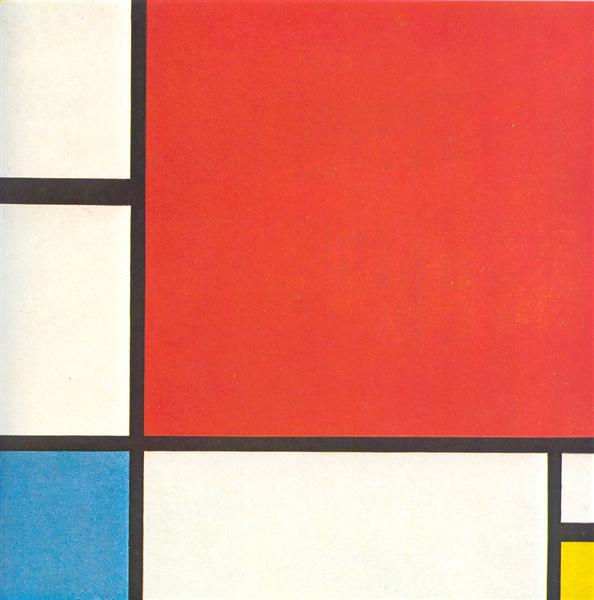
\includegraphics[width=.5\textwidth]{articles/04-matematica-na-arte--/figura2.jpeg}%
        \caption*{Fonte: \url{http://cultura.culturamix.com/arte/obras-de-piet-mondrian}}%
        \label{fig:composicaoII}%
    \end{figure}%
    
    \begin{figure}[ht]%
        \centering%
        \caption{Piet Mondrian, \textit{Composition A.}}%
        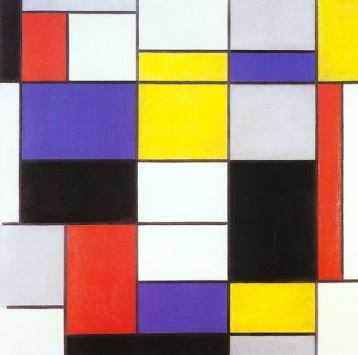
\includegraphics[width=.5\textwidth]{articles/04-matematica-na-arte--/figura3.jpeg}%
        \caption*{Fonte: \url{http://cultura.culturamix.com/arte/obras-de-piet-mondrian}}%
        \label{fig:composition-a}%
    \end{figure}%


    \begin{figure}[ht]%
        \centering%
        \caption{Wassily Kandinsky, \textit{Arch and Point.}}%
        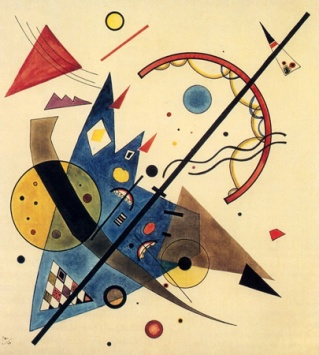
\includegraphics[width=.5\textwidth]{articles/04-matematica-na-arte--/figura4.jpeg}%
        \caption*{Fonte: \url{https://www.todocuadros.es/pintores-famosos/kandinsky/}}%
        \label{fig:arch-and-point}%
    \end{figure}%

    \begin{figure}[ht]%
        \centering%
        \caption{Wassily Kandinsky, \textit{On the points.}}%
        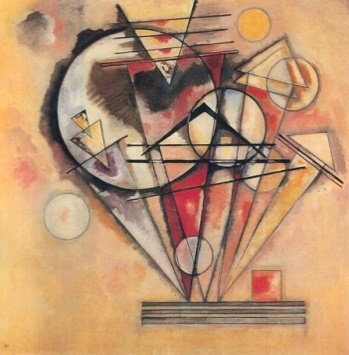
\includegraphics[width=.5\textwidth]{articles/04-matematica-na-arte--/figura5.jpeg}%
        \caption*{Fonte: \url{https://www.todocuadros.es/pintores-famosos/kandinsky/}}%
        \label{fig:on-the-point}%
    \end{figure}%

    No segundo momento iniciamos a aula expositiva com uma breve retomada. Nesta atividade objetivamos estimular a percepção visual por meio de cores e formas, bem como desenvolver o raciocínio a partir da prática da comparação, análise, identificação e a classificação das figuras planas presentes na tela em questão.  

    Apresentamos aqui as transcrições de alguns comentários dos alunos durante a realização da prática: “Eu nunca fiz tarefas de matemática utilizando telas de pintura ou figuras e, pensei que isso seria difícil”; “Não consigo formar novas figuras geométricas, pois elas já estavam todas formadas”; “Professor, não estou conseguindo mais me lembrar dos quadriláteros que estudamos na aula passada”; “Vai ser difícil, pois não sou artista”.  

    Dessa forma, na continuidade das atividades, realizamos algumas perguntas pertinentes ao conteúdo de Geometria, para gerar um debate, e assim surgirem as problemáticas a serem investigadas, entre elas, temos: O que é um quadrilátero? Quais os quadriláteros por nós estudados? O que diferencia um quadrado de um retângulo? Como são classificados os triângulos quanto aos lados? E, após essa breve discussão, novas dúvidas foram geradas e outras minimizadas, e aquela hesitação inicial diante da tarefa apresentada deu lugar à autoconfiança, que proporcionou uma mudança de atitude na qual propiciou a retomada da atividade proposta, como bem mostra a Figura \ref{fig:aluno-durante-pratica}.

    \begin{figure}[ht]%
        \centering%
        \caption{Aluno durante a prática da primeira atividade}%
        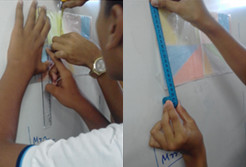
\includegraphics[width=.6\textwidth]{articles/04-matematica-na-arte--/figura6.jpg}%
        \caption*{Fonte: Elaborado pelo autor}%
        \label{fig:aluno-durante-pratica}%
    \end{figure}%

    O terceiro momento foi iniciado com um debate objetivando desenvolver a capacidade de observação e comparação entre os objetos e formas presentes no cotidiano dos alunos, mostrando a intensa presença da Matemática no mundo em que vivemos bem como, o quanto a Geometria apresenta-se envolvida ao nosso entorno, assim como despertar nos alunos o senso crítico para refletirem sobre como os artistas plásticos poderiam se beneficiar dos conhecimentos geométricos quando do desempenho de suas atividades profissionais.  

    Em seguida, apresentamos a atividade que teria como base as seis telas pintadas a óleo e elaboradas pelo pesquisador. Nessa atividade pedimos que os grupos identificassem as figuras planas presente nas obras e medissem o seu perímetro, como exemplificado na Figura \ref{fig:alunos-durante-2a-pratica}.

    \begin{figure}[ht]%
        \centering%
        \caption{Alunos durante a prática da segunda atividade}%
        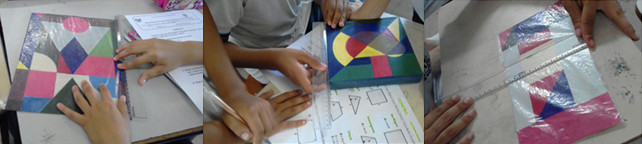
\includegraphics[width=.90\textwidth]{articles/04-matematica-na-arte--/figura7.jpg}%
        \caption*{Fonte: Elaborado pelo autor}%
        \label{fig:alunos-durante-2a-pratica}%
    \end{figure}%

    No quarto momento continuamos o estudo apresentando os conceitos de ângulos internos e de como medi-los por meio de um transferidor, bem como aferir dimensões utilizando régua, trena e fita métrica. Além de ensiná-los como proceder para executar os cálculos de área e de perímetro das principais figuras planas estudadas. Vale salientar que neste encontro utilizamos novamente as composições de Mondrian e Kandinsky com o propósito de justificar a importância dos conhecimentos geométricos para o processo criativo de tais pintores, além de proporcionar um momento de reflexão a respeito de como a Arte pode interagir com a Matemática e, no caso particular, com a Geometria.  

    Como essa forma de desenvolver os conteúdos causou um pouco de estranheza aos discentes, eles conseguiram assimilar bem nossa proposta e percebemos que nas turmas investigadas, no que se refere à desenvoltura apresentada ao longo das discussões, consideramos que o resultado foi bastante satisfatório, visto que emergiram consideráveis reflexões ao longo do debate. E esse fato deve ser levado em consideração, uma vez que estávamos lidando com alunos do 6º ano, recém-chegados às séries do Ensino Fundamental, anos finais, que tem uma estrutura de tempo e espaço diferente dos anos iniciais. 

    Quanto ao desempenho dos investigados durante a realização das atividades, constatamos que a proposta propiciou o desenvolvimento satisfatório da compreensão acerca das figuras geométricas e de suas aplicações no cotidiano das pessoas. Salientamos que, quanto à aferição de medidas de ângulos por meio do uso do transferidor, verificamos certa dificuldade que poderia ser justificada pelo fato de os alunos desconhecerem, até aquele momento, o referido instrumento de medida, bem como utilizá-lo. 

    No quinto momento, após a realização de algumas atividades práticas de verificação de medidas, utilizando-se de fita métrica, transferidor, trena e régua. Solicitamos que utilizassem o espaço da sala de aula e dos objetos, além das obras para realizar novas medições e fazer o cálculo de áreas, perímetro e ângulos. 

    Percebemos uma boa evolução no que diz respeito à interação e ao senso de cooperação dos alunos, visto que a resistência de alguns alunos de interagir com a sua equipe durante execução da atividade havia diminuído sensivelmente. Constatamos também, que a dificuldade apresentada, em momentos anteriores, para se verificar a medida de um ângulo interno de uma figura plana, utilizando o transferidor, já não existia. A Figura \ref{fig:alunos-durante-3a-pratica} nos dá uma breve noção do exposto anteriormente. 

    \begin{figure}[ht]%
        \centering%
        \caption{Alunos durante a prática da terceira atividade}%
        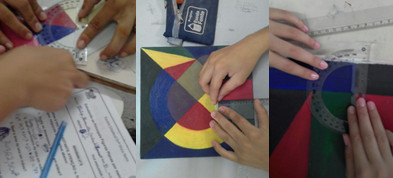
\includegraphics[width=.80\textwidth]{articles/04-matematica-na-arte--/figura8.jpg}%
        \caption*{Fonte: Elaborado pelo autor}%
        \label{fig:alunos-durante-3a-pratica}%
    \end{figure}%

    No sexto momento abrimos espaço aos alunos para que eles avaliassem a atividade realizada na aula anterior. A discussão foi bastante interessante, pois os investigados tiveram oportunidade de refletir sobre a importância de conhecer os conceitos geométricos referentes às figuras planas e, também, de como a utilização desse conhecimento poderia ser útil para a realização de diversas atividades do nosso dia a dia. Tudo isso, despertou o interesse dos alunos em tentar relacionar aqueles conteúdos estudados com a realidade de cada um.  

    Apresentamos aqui seis comentários proferidos pelos alunos: “Foi bom aprender como se medir usando a fita métrica e a trena”; “Saber calcular área e perímetro é importante para um engenheiro”; “Foi legal aprender como se usa um transferidor”; “Gostei muito de trabalhar usando uma fita métrica”; “Algumas coisas que a gente tem em casa podem ser medidas com uma trena”; “Saber usar uma trena é muito importante quando se quer verificar as medidas de um terreno ou de uma parede”. 

    A discussão realizada propiciou a retomada dos conteúdos apresentados ao longo dos encontros anteriores proporcionando o aprofundamento do debate em torno da aplicação dos conhecimentos de Geometria no dia a dia das pessoas bem como na área profissional, além disso, viabilizou um momento para que todos os participantes do estudo estabelecessem conexões entre os conteúdos apresentados em sala e os diversos ramos do conhecimento.  

    Por meio dessa ação os alunos observados tiveram a oportunidade de perceber a Geometria como uma ferramenta presente além dos muros da escola. Outro ponto a ser destacado desse momento diz respeito à possibilidade dada aos alunos de vislumbrarem o relevante papel que a Geometria desempenha na vida cotidiana do ser humano podendo ser considerada como ferramenta fundamental no processo de interação do indivíduo com o seu meio. Vale salientar que os conhecimentos inerentes à Geometria, além de constituírem a parte intuitiva da disciplina de Matemática, eles estão intimamente ligados à realidade das pessoas. 

    Após a realização do debate, propusemos uma rápida atividade prática de medição, como retratada na Figura \ref{fig:alunos-durante-6a-pratica}. Nessa atividade todos os grupos deveriam medir as dimensões da janela e da porta existentes na sala de aula usando como ferramenta de aferição uma trena ou uma fita métrica e, em seguida, realizariam o cálculo do perímetro e da área das referidas esquadrias.  

    \begin{figure}[ht]%
        \centering%
        \caption{Alunos durante a prática no sexto momento da pesquisa}%
        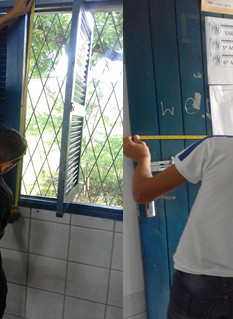
\includegraphics[width=.25\textwidth]{articles/04-matematica-na-arte--/figura9.jpg}%
        \caption*{Fonte: Elaborado pelo autor}%
        \label{fig:alunos-durante-6a-pratica}%
    \end{figure}%

    Essa atividade foi interessante, uma vez que os grupos tiveram a oportunidade de verificar que, devido a pequenas diferenças no que diz respeito ao trabalho de aferição das dimensões da janela e da porta, os valores calculados para o perímetro e para a área não foram exatamente iguais entre os respectivos grupos, apresentavam algumas diferenças de aproximadamente entre um centímetro a dois centímetros, mas nada que preocupasse tanto, pois entendemos que nossos instrumentos de medidas são rudimentares e o seu manuseio pode levar a pequenas diferenças de medidas. 

    Mas, isso nos deu a oportunidade de evidenciar para os alunos participantes da investigação da importância de executar uma aferição cuidadosa, uma vez que, ao aferirmos erroneamente uma determinada medida, iremos comprometer os resultados finais do nosso trabalho, e pode também nos levar a perda de materiais, caso fizéssemos uma maquete para representar nossos estudos de sala de aula. 

    Já no sétimo momento, tínhamos por objetivo estimular o viés artístico de cada um dos alunos, pois na referida atividade, constava uma questão que solicitava a composição de um desenho no qual o tema seria figuras planas. E ainda, solicitamos que observassem os ambientes fora da escola e anotassem os objetos identificados e associados com as figuras geométricas. 

    De início, realizamos uma discussão a respeito da presença de elementos geométricos no nosso cotidiano. Listamos, a critério de elucidação positiva dos momentos vivenciados ao longo do processo, oito comentários dos alunos: “Eu vejo figuras planas em muitos prédios”; “A geometria está presente em praças e calçadas da cidade”; “As portas, janelas e portões das casas têm forma de retângulos e quadrados que são figuras planas”; “Têm muitas figuras geométricas em minha casa”; “Muitas coisas que encontramos na rua, possuem as formas geométricas que aprendemos aqui nessas aulas”; “As formas geométricas estão presentes nos azulejos das paredes da cozinha de minha casa”; “As placas de trânsito têm as formas de triângulo, de quadrado e de círculo”; “Muitos artistas utilizam os conhecimentos de Geometria para fazer suas telas”. 

    E, no nosso oitavo momento foi realizado um debate rico pela troca de experiências vivenciadas e de reflexão a respeito das novas descobertas. Eis aqui em destaque oito comentários proferidos pelos alunos: “Essa última atividade foi boa porque a gente viu as figuras planas em muitos prédios”; “Achei legal essa atividade porque aprendemos a fazer desenhos, usando muitas figuras planas do jeito que os artistas famosos fazem”; “Gostei dessa atividade porque aprendi sobre a importância das figuras planas para os engenheiros”; “As figuras planas estão em muitos objetos de nossas casas”; “Gostei de saber como é importante usar corretamente uma trena”; “Estudar figuras planas foi importante porque a Geometria está presente na nossa vida”; “Esta atividade foi legal porque vimos na prática como os artistas podem utilizar os conhecimentos de geometria para realizar as suas obras”; “Gostei de saber que até nas Artes têm Matemática”.  

    Realizamos uma culminância das atividades desenvolvidas, assim oportunizamos os grupos a apresentarem as suas composições, colocamos a representação de algumas delas na Figura \ref{fig:composicoes-3-grupos}. 

    \begin{figure}[ht]%
        \centering%
        \caption{Composições elaboradas por três dos grupos participantes.}%
        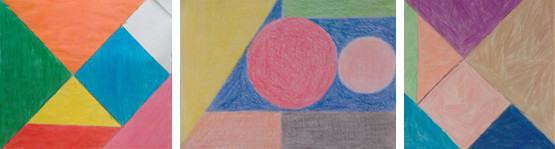
\includegraphics[width=.90\textwidth]{articles/04-matematica-na-arte--/figura10.jpg}%
        \caption*{Fonte: Elaborado pelo autor}%
        \label{fig:composicoes-3-grupos}%
    \end{figure}%

    \section{Considerações finais}

    A análise do processo desenvolvido evidenciou como a Arte pode contribuir no ensino e aprendizagem de Geometria. Uma vez que a utilização de pinturas em sala foi satisfatória, visto que o procedimento promoveu o interesse do aluno pela discussão em torno da importância dos conhecimentos geométricos para outras áreas do conhecimento. Percebemos também que, a utilização de telas de pintores renomados nas aulas, proporcionou ao aluno uma modificação do seu olhar no que diz respeito à importância da Geometria para o desempenho de muitas atividades do nosso cotidiano, tais como: a aferição de medidas de dimensão, o cálculo de áreas e de perímetros, dentre outros saberes.  

    Com esta proposta, também foi dada a oportunidade de se discutir, por exemplo, como o conhecimento geométrico pode ser útil para um artista durante o processo de composição de uma obra, propiciando assim, um pensar sobre a Geometria como algo de grande utilidade presente na nossa vida. 

    Os resultados advindos desta pesquisa mostram que, ao longo de todo o processo, os alunos apresentaram alterações, tanto no interesse quanto na participação, pois foi percebida uma mudança positiva de atitude, principalmente, daqueles que apresentavam um comportamento menos participativo em nossas aulas. Isso, pois, durante as atividades os alunos manifestaram seus questionamentos, ideias e reflexões a respeito das possibilidades de utilização dos conceitos geométricos referentes às figuras planas no nosso cotidiano.   

    Outro ponto a ser destacado diz respeito à Arte como facilitadora do processo ensino e aprendizagem, visto que, devido ao seu viés estético e lúdico o recurso da Arte mostrou-se como valioso elemento para o ensino da Geometria como também para a construção do saber de cada um dos envolvidos no processo, pois ao dar oportunidade de manusearem diferentes instrumentos de medidas, propiciou a construção de um ambiente de discussão no qual contribuiu tanto para a ampliação dos conhecimentos quanto para desenvolvimento da habilidade de expressar opinião, ou seja, de argumentação, como também desenvolveu, em cada um dos envolvidos, as habilidades artísticas, visto que uma das atividades propostas aos investigados era a criação de uma obra a ser realizada em grupo e cujo tema girava em torno das figuras geométricas estudadas durante o processo.  

    Não identificamos limitações para a utilização da Arte como caminho para o ensino e aprendizagem da Matemática. Percebemos que as aprendizagens apresentaram bons resultados, quanto a assimilação dos conteúdos, e apontamos que isso aconteceu devido a forma com que foram desenvolvidas as atividades, por meio da experimentação, e utilizando a observação e o contato com as formas geométricas, além de poderem ter tido a oportunidades de utilizar alguns instrumentos medidas tanto para verificar as figuras dos quadros como para se inspirarem e produzirem suas pinturas autorais. 

    Esperamos que esse artigo sirva de inspiração para todos aqueles profissionais que trabalham com educação de jovens em um contexto similar ao investigado nessa pesquisa e que desejam utilizar a Arte como uma possível aliada ao ensino da Matemática, em especial, ao Ensino da Geometria, pois, mesmo que não sejamos profundos conhecedores dessa área de conhecimento, todos nós temos plenas condições de propiciar algo de relevância que nos possibilite viabilizar relações significantes entre a área da Arte e da Matemática, e que sejam capazes de contribuir na apropriação de novos conceitos e demandas surgidas durante o processo de ensino e aprendizagem da Matemática, e em especial, a Geometria. 

    \printbibliography[heading=subbibliography,notcategory=fullcited]

    \label{chap:matematicanaarteend}

\end{refsection}

\begin{refsection}
    \renewcommand{\thefigure}{\arabic{figure}}
    
    \chapterTwoLines
    {O material dourado como recurso didático no ensino do algoritmo da subtração}
    {Uma experiência em sala de aula}
    \label{chap:material-dourado}

    \begin{otherlanguage}{english}

    \fakeChapterTwoLines
    {The golden material as a didactic resource in the subtraction algorithm teaching}
    {A classroom experience}

    \end{otherlanguage}
    
    \articleAuthor
    {Verônica Umbelino Souza de Carvalho}
    {\textit{Minicurrículo e contato não disponibilizados pela autora.}}
    
    \articleAuthor
    {Anilda Pereira da Silva Guimarães}
    {Graduada em Ciências com habilitação em Matemática pela Universidade Federal do Rio Grande do Norte (1981). Graduada em Pedagogia pela Universidade Federal do Rio Grande do Norte (1987). Mestra em Educação pela Universidade Federal do Rio Grande do Norte (2005). Atualmente é professora do Instituto de Educação Superior Presidente Kennedy. ID Lattes: 9681.3290.9483.0259.}
    
    \begin{galoResumo}
        \marginpar{
            \begin{flushleft}
            \tiny \sffamily
            Como referenciar?\\\fullcite{SelfCarvalhoAndGuimarães2021material}\mybibexclude{SelfCarvalhoAndGuimarães2021material}, p. \pageref{chap:material-dourado}--\pageref{chap:material-douradoend}, \journalPubDate{}
            \end{flushleft}
        }
        A questão que norteia este estudo é uma experiência realizada com a utilização do Material Dourado como facilitador da compreensão da subtração com reserva, numa turma do 4º ano do Ensino Fundamental de uma escola estadual localizada no município de Santa Cruz/RN. Esse trabalho foi motivado por tanto presenciar nas reuniões pedagógicas, a angústia de alguns professores relatando as dificuldades que seus alunos apresentam para compreender o algoritmo da subtração, em especial, a subtração com reserva. A pesquisa foi desenvolvida com base na pesquisa ação, onde buscamos aplicar algumas atividades de intervenção didática. O referencial teórico em que se baseou esse estudo aborda a importância dos materiais manipuláveis, em particular o Material Dourado, para uma melhor compreensão nos aspectos ensino/aprendizagem da Matemática. Assim, recorremos a \textcite{NACARATO2005trabalho}, \textcite{BERTONAndITACARAMBI2009Números}, \textcite{LORENZATO2006Começar}, \textcite{CENTURIÓN1995Números}, dentre outros, por reconhecerem a importância do uso do material concreto como um recurso didático facilitador no processo de ensino e aprendizagem. Podemos concluir que o uso do Material Dourado no ensino da matemática, além de facilitar a compreensão do desagrupamento na subtração, dá às relações numéricas abstratas uma imagem mais concreta, facilitando a compreensão, o desenvolvimento do raciocínio lógico, tornando o aprendizado bem mais agradável, pois é dada ao aluno a oportunidade de construir seus conhecimentos de uma forma mais interativa, dinâmica e prazerosa.
    \end{galoResumo}
    
    \galoPalavrasChave{Material Dourado. Algoritmo da subtração. Aprendizagem.}
    
    \begin{otherlanguage}{english}

    \begin{galoResumo}[Abstract]
        The issue that guides this paper is an experience carried out with the use of the golden material as a facilitator to understand the subtraction with reserve in a 4th grade classroom from the elementary school in a public state school located in Santa Cruz/RN region. This paper has been motivated after attending during pedagogical meeting the anguish of some teachers who reported the difficulties their students had in order to understand the subtraction algorithm. In particular, the subtraction with reserve. The research was developed based on the action research, where we sought to apply some didactic intervention activities. The theoretical reference in which this paper was based on approaches the importance of manipulable materials, in particular, the golden material, for a better comprehension related to the teaching learning of mathematics. Thus, we had as support \textcite{NACARATO2005trabalho}, \textcite{BERTONAndITACARAMBI2009Números}, \textcite{LORENZATO2006Começar}, \textcite{CENTURIÓN1995Números}, among others, since they recognize the importance of the use of a solid material as a didactic resource on the teaching and learning process. We can conclude that the use of the golden material in the mathematics teaching, in addition to make the comprehension/understanding of the subtraction ungrouping easier. By giving the abstracts numerical relation a more concrete image, facilitating the understanding, logical thinking development, making the learning enjoyable, since it gives the students the opportunity to build their knowledge in a more interactive, dynamic and enjoyable way. 
    \end{galoResumo}
    
    \galoPalavrasChave[Keywords]{Golden Material. Subtraction Algorithm. Learning.}
    \end{otherlanguage}

    \section{Introdução}

    A Matemática é uma disciplina que está presente em todos os níveis da educação, e é considerada pela maioria das instituições escolares a disciplina que causa o maior índice de reprovação e, consequentemente, o desinteresse por parte dos educandos por essa área do conhecimento. Para agravar ainda mais essa situação, a prática educativa no ensino da Matemática muitas vezes é realizada na sala de aula de forma abstrata e descontextualizada da realidade do educando, visto que geralmente o professor adota procedimentos, tais como: expor e/ou explicar o conteúdo; passar uma lista de exercícios; e fazer a correção destes. Sobre isso, Lorenzato afirma: Palavras não alcançam o mesmo efeito que conseguem os objetos ou imagens, estáticas ou em movimento. Palavras auxiliam, mas não são suficientes para ensinar. [\dots] o fazer é mais forte que o ver ou ouvir [\dots] \cite[p.~17--18]{LORENZATO2006Começar}. 

    Sabe-se que a Matemática se constitui em um saber que está presente nas ações do dia a dia, por isso uma inquietação/indagação motivou a pesquisa: por que um saber tão presente nas decisões do cotidiano é objeto de retenção na escola? Intervir nessa realidade de modo a encontrar novas formas de abordagem no processo ensino-aprendizagem da Matemática tornou-se um desafio. Certamente, são inúmeras as dificuldades encontradas no ensino e aprendizagem desta disciplina, mas aqui o objetivo consiste em analisar como o Material Dourado pode contribuir para a aprendizagem da subtração com reserva numa turma do 4º ano do Ensino Fundamental. 

    Os procedimentos metodológicos necessários à realização deste trabalho foram realizados na perspectiva da pesquisa ação, trabalhando a matemática de maneira construtiva e significativa através de uma sequência de atividades com o uso do Material Dourado. Esse material pode ser encontrado na maioria das escolas públicas do Brasil, porém, muitas vezes fica obsoleto em algum espaço escolar porque a maioria dos professores não sabe utilizá-lo, ou não acredita que o uso deste material, mediado pelo professor, possa contribuir significativamente para a aprendizagem. Os sujeitos desta pesquisa foram os alunos do 4º ano --- turno vespertino --- da Escola Estadual Isabel Oscarlina Marques, localizada no município de Santa Cruz/RN. 

    O referencial teórico que embasa esta pesquisa aponta a importância dos materiais manipuláveis, em particular o Material Dourado, para uma melhor compreensão dos conceitos matemáticos ligados às operações fundamentais e a sua relação no aspecto ensino/aprendizagem da Matemática. Assim, recorre-se a \textcite{NACARATO2005trabalho}, \textcite{BERTONAndITACARAMBI2009Números}, \textcite{CENTURIÓN1995Números} e \textcite{LORENZATO2006Começar}, entre outros. Busca-se através destes teóricos fundamentar a relevância de trabalhar com material concreto para o desenvolvimento do raciocínio lógico-matemático da criança.  

    Os problemas de aprendizagem da Matemática no Ensino Fundamental tratados neste trabalho dizem respeito aos fatores que contribuem para que a Matemática seja vista como uma disciplina cansativa e com maior índice de reprovação. Tornar suas aulas mais lúdicas, com atividades que disponibilizem o uso de materiais concretos, apresentando questões que partam da realidade do aluno foi a proposta utilizada nessa pesquisa para se chegar a um resultado mais satisfatório.  

    Entende-se que cabe ao educador por meio da intervenção pedagógica propiciar atividades que levem a uma aprendizagem significativa. Para que isso ocorra é necessário que o professor reflita sobre sua prática pedagógica, compreendendo o aluno como alguém que pode sentir prazer em aprender e não como um mero executor de tarefas.  

    Ensinar exige reflexões para que se contribua significativamente na formação de cidadãos que atendam as demandas do século XXI. Nessa perspectiva, desencadeou-se esse estudo, tendo como foco o uso do Material Dourado no ensejo de facilitar a aprendizagem da subtração com reserva através do uso desse material. 

    Para melhor compreensão, organiza-se este trabalho em cinco seções: A primeira, a introdução, onde situam-se o tema, o objetivo e a metodologia utilizada. A segunda seção traz um resgate teórico a respeito do uso do Material Dourado como recurso didático. A terceira discorre sobre o algoritmo da subtração. A quarta seção enfoca a experiência vivenciada na turma do 4º ano, relatando cada encontro realizado e, por fim, a quinta tece as considerações finais sobre a pesquisa realizada.

    \section{Material dourado: o que dizem alguns teóricos}

    \textcite{BERTONAndITACARAMBI2009Números} afirmam que Montessori criou o Material Dourado para trabalhar aritmética com as crianças que apresentavam distúrbios de aprendizagem. O nome dourado se deve à versão original que era feita com contas douradas. Quando foi industrializado, esse material passou a ser feito de madeira, mantendo o nome original. O material é constituído por cubinhos, barras, placas e o cubo, apresentando as regras de agrupamento na base 10. A manipulação e uso desse recurso podem ajudar na compreensão das operações fundamentais, reforçando a noção de troca no sistema posicional.  

    O Material Dourado propicia aos alunos descobrirem as relações entre as peças que o compõe, a saber: uma barra tem dez cubinhos, uma placa tem dez barras e o cubo tem dez placas. Isso é constituído para representar um sistema de agrupamento, associando o modelo didático com o conceito matemático. 

    No princípio, esse material foi criado com o intuito de auxiliar nas atividades que propiciassem o ensino e a aprendizagem do sistema de numeração decimal-posicional e, consequentemente, em métodos para efetuar as operações fundamentais. Hoje pode ser utilizado para o estudo de frações, conceituação e cálculo de áreas e volumes, trabalho com números decimais, raiz quadrada entre outros. Nesta pesquisa utilizou-se o Material Dourado para se trabalhar a subtração com reserva, objeto desse estudo. Atualmente, o material é apresentado conforme a Figura \ref{fig:material-dourado}.

    \begin{figure}[ht]%
        \centering%
        \caption{Material Dourado}%
        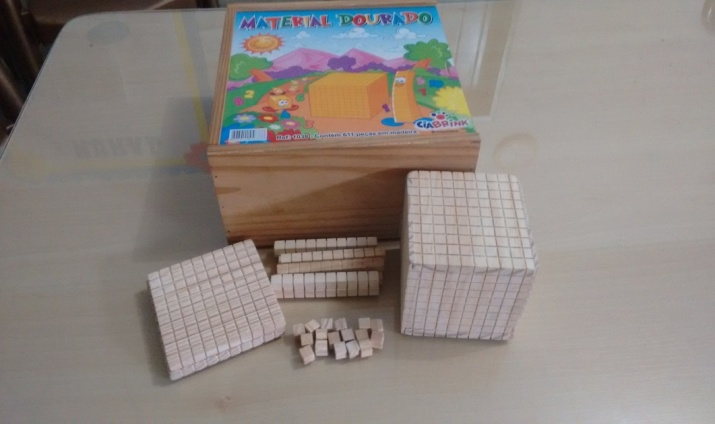
\includegraphics[width=.5\textwidth]{articles/05-material-dourado-com/figura1.jpeg}%
        \caption*{Fonte: Arquivo pessoal.}%
        \label{fig:material-dourado}%
    \end{figure}%

    O Material Dourado é um recurso didático riquíssimo, pois além de ser muito versátil ele tem como base ideológica primordial a educação sensorial da criança, a qual pode ser elencada, segundo \cite[p.~2]{DALTOÉAndStrelowTrabalhando} da seguinte forma:

    \begin{enumerate}
        \item desenvolve na criança a independência, a confiança em si mesma, a concentração, a coordenação e a ordem; 
        \item gera e desenvolve experiências concretas estruturadas para conduzir, gradualmente, a abstrações cada vez maiores;
        \item faz a criança, por ela mesma, perceber os possíveis erros que comete ao realizar uma determinada ação com o material; 
        \item trabalha com os sentidos da criança.
    \end{enumerate}

    Em outras palavras o Material Dourado desenvolve o raciocínio do aluno, estimula o pensamento lógico-matemático e faz com que o educando aprenda com prazer, assim, as informações que obtém não esquece tão facilmente. Por ser um material de fácil manipulação, o Material Dourado fornece condições para que o aluno absorva com mais facilidade a proposta de ensino-apren\-di\-za\-gem que o professor apresenta. Isso nos faz reportar novamente a Daltoé \& Strelow, quando enfoca que: O material dourado destina-se a atividades que auxiliam o ensino e a aprendizagem de sistema de numeração decimal-posicional e dos métodos para efetuar as operações fundamentais. \cite[p.~3]{DALTOÉAndStrelowTrabalhando}.

    O uso desse material é importante porque ao manusear as peças o aluno passa do abstrato para o concreto, facilitando a compreensão, o desenvolvimento do raciocínio lógico, o que torna o aprendizado bem mais agradável e sólido. Com sua utilização em sala de aula, os alunos dos anos/séries iniciais do ensino fundamental conseguem entender melhor a subtração com reserva. Considera-se, pois, que esses alunos ainda têm certa dificuldade de entender a transição do abstrato para o concreto, assim, o uso desse material possibilita uma aprendizagem mais significativa e eficaz. 

    Os PCN de Matemática afirmam que: “Os [\dots] recursos didáticos como livros, vídeos, televisão, rádio, calculadora, computadores, jogos e outros materiais têm um papel importante no processo de ensino e aprendizagem”. \cite[p.~57]{ParâmetrosCurricularesMatematica1998}.

    Contudo, estes recursos precisam estar integrados a situações que levem ao exercício da análise e da reflexão. Isso significa que o ensino de Matemática com materiais manipulativos não deve se reduzir a uma transposição meramente qualitativa. O aluno precisa ser capaz de estabelecer semelhanças e diferenças, perceber regularidades e singularidades, estabelecer relações com outros conhecimentos e com a vida cotidiana e compreender as representações simbólicas da Matemática.  

    Nesse sentido, é de suma importância ressaltar que o ensino e a aprendizagem com material concreto é o início de um processo de construção de conhecimentos, pois segundo \textcite[p.~20]{LORENZATO2006Começar}, “O concreto palpável possibilita apenas o primeiro conhecimento, isto é, o concreto é necessário para a aprendizagem inicial, embora não seja suficiente para que aconteça a abstração matemática”.

    Assim, o professor não deve utilizar o Material Dourado como único recurso para trabalhar um conteúdo, ele precisa ter o cuidado de estimular reflexões e discussões para que o aprendizado se dê por completo.  

    Vale salientar que esses materiais não devem ser vistos apenas como “brincadeira”, até podem ser considerados como tal, apenas pelos alunos, mas para os docentes são uma ferramenta importante, com objetivos definidos, como por exemplo, utilizar como instrumento para proporcionar um processo de ensino e aprendizagem com qualidade, tornando suas aulas mais interessantes, atrativas, participativas e principalmente significativas, pois ao fazer o uso do concreto os alunos estarão aprendendo através do que estão vivenciando, ou seja, da ação. Entretanto, \textcite[p.~5]{NACARATO2005trabalho} nos lembra que: “Nenhum material didático --- manipulável ou de outra natureza --- constitui a salvação para a melhoria do ensino de Matemática. Sua eficácia ou não dependerá da forma como ele for utilizado”. 

    No ensino tradicional\footnote{No ensino tradicional, a aprendizagem do aluno era considerada passiva, consistindo basicamente em memorização de regras e fórmulas. Para a maioria dos professores desta escola o uso de materiais ou objetos era considerado pura perda de tempo, uma atividade que perturbava o silêncio ou a disciplina da classe. Os poucos que os aceitavam e utilizavam o faziam de maneira puramente demonstrativa, servindo apenas de auxiliar à exposição, à visualização e à memorização do aluno. Exemplos disso são: o flanelógrafo, as réplicas grandes em madeira de figuras geométricas, desenhos ou cartazes fixados nas paredes.}, as crianças acabam ``dominando'' os algoritmos a partir de treinos cansativos, mas sem conseguirem compreender o que fazem. Com o Material Dourado a situação é outra: as relações numéricas abstratas passam a ter uma imagem concreta, facilitando a compreensão. Obtém-se, então, além da compreensão dos algoritmos, um notável desenvolvimento do raciocínio e um aprendizado bem mais agradável.  

    Piaget nos esclarece que: Os jogos e os materiais manipuláveis não são apenas uma forma de divertimento, mas são meios que contribuem e enriquecem o desenvolvimento intelectual. Para manter seu equilíbrio com o mundo, a criança necessita brincar, criar, jogar e inventar (PIAGET 1989, p.~5).

    Esta pesquisa nos fez perceber que os materiais manipulativos se constituem em formas interessantes de propor problemas, pois permitem que estes sejam apresentados de modo atrativo e favorecem a criatividade na elaboração de estratégias de resolução e busca de soluções. Foi com esta preocupação que se desenvolveu este trabalho.

    \section{Algoritmo da subtração}

    É importante lembrar que o termo algoritmo é definido por \textcite[p.~150]{CENTURIÓN1995Números} como “uma sequência de etapas, que fazem parte de uma instrução exata a ser seguida”.

    Assim, para resolver subtrações com reserva, quando um ou mais algarismos do minuendo é menor que o do subtraendo, há dois métodos: um, mais antigo: Método da Compensação, que consiste em adicionar quantidades iguais no minuendo e no subtraendo. Utilizava-se, então, o Teorema da Invariância do Resto, ou seja, numa subtração, se adicionarmos o mesmo número ao minuendo e ao subtraendo a diferença não se altera. Essa ideia pode ser sintetizada assim: na subtração de dois números, sempre que ambos são acrescidos da mesma quantidade, a diferença entre eles permanece inalterada.  

    Em outras palavras o aumento do primeiro número é compensado pelo aumento do segundo número. Daí o nome propriedade da compensação. Assim, por exemplo, a diferença entre 374 e 158 é igual à diferença entre 384 e 168, pois ambos os números foram aumentados em uma dezena. Veja:

    \begin{center}
        \hspace{90pt}
        \begin{tikzpicture}
            \node[anchor=south] (toptable) at (0, 0)
                {\begin{tabular}{P{18pt} | P{18pt} | P{18pt}}
                    $C$ & $D$ & $U$ \\ \hline
                    $3$ & $7$ & $4$ \\
                    $\mathllap-1$ & $5$ & $8$ \\ \hline
                    2 & 1 & 6
                \end{tabular}};
            \node[anchor=north] (bottable) at ([yshift=-72pt]toptable.south)
                {\begin{tabular}{P{18pt} | P{18pt} | P{18pt}}
                    $C$ & $D$ & $U$ \\ \hline
                    $3$ & \boldmath$8$ & $4$ \\
                    $\mathllap-1$ & \boldmath$6$ & $8$ \\ \hline
                    2 & 1 & 6
                \end{tabular}};
            \draw [-{To[width=7pt,length=5pt]}] ([yshift=-10pt]toptable.south) -- ([yshift=10pt]bottable.north);
            \node[anchor=west,align=left] (text) at ([yshift=-36pt,xshift=10px]toptable.south)
                {Aumentando uma dezena\\no minuendo e no subtraendo};
        \end{tikzpicture}
    \end{center}

    Na subtração por compensação quando adicionamos uma dezena (ou seja, 10 unidades) no minuendo, na ordem das unidades, temos que adicionar uma dezena na ordem das dezenas, no subtraendo. É como no exemplo abaixo, ao adicionar 10 unidades ao minuendo temos que adicionar 1 dezena (que é o mesmo que 10 unidades) ao subtraendo para que o resultado não se altere. 

    Desse modo, para realizar a subtração $384 - 168$ pensa-se da seguinte forma: Como de 4 não podemos tirar 8, dizemos 8 para 14, e vai 1 (este 1 é a dezena que compensamos no subtraendo por termos adicionado uma dezena no minuendo).

    \begin{center}       
        \begin{tikzpicture}
            \node[anchor=south] (toptable) at (0, 0)
                {\begin{tabular}{P{18pt} | P{18pt} | P{18pt}}
                    $C$ & $D$ & $U$ \\ \hline
                    $3$ & $8$ & $4^{\mathrlap{+10}}$ \\
                    $\mathllap-1$ & $6^{\mathrlap{+1}}$ & $8$ \\ \hline
                    2 & 1 & 6
                \end{tabular}};
        \end{tikzpicture}
    \end{center}

    Como se pôde verificar, $384 - 168$ é igual a $216$. Esse método da compensação baseia-se em técnicas não muito elementares que carregam em si o caráter de “decorar”, ou automação. Já o método da decomposição que envolve a troca é feito através da decomposição do minuendo a partir do desagrupamento (e reagrupamento).

    Esse método requer compreensão de características do sistema de numeração decimal (SND), em especial a noção de valor posicional e agrupamentos na base 10. Pode ser representado concretamente com Material Dourado e é o que mais se encontra nas propostas metodológicas de livros didáticos atuais. Ou seja, o método que predomina no ensino atualmente, consiste na decomposição do minuendo e supõe uma compreensão clara dos valores relativos dos algarismos e do Sistema de Numeração Decimal de modo geral.  

    A opção atual pela decomposição, certamente deve-se ao fato dessa técnica ser mais facilmente concretizável para as crianças, tornando possível a compreensão dessa de modo mais eficiente no ensino e na aprendizagem da Matemática. Na Subtração por decomposição (representada abaixo) pensa-se da seguinte forma: como de 4 não se pode tirar 8, troca-se uma dezena por 10 unidades e adiciona-se às unidades (ficando 14); assim, ficam 7 dezenas na ordem das dezenas e 14 unidades na ordem das unidades. Depois se diz 14 tirando 8 e coloca-se o 6 na ordem das unidades; 7 dezenas menos 6 dezenas, colocando-se o 1 na ordem das dezenas e, por fim, 3 centenas menos 1 centena igual a duas centenas, resultando o 2 na ordem das centenas. Veja:

    \begin{center}       
        \begin{tikzpicture}
            \node[anchor=south] (toptable) at (0, 0)
                {\begin{tabular}{P{18pt} | P{18pt} | P{18pt}}
                    $C$ & $D$ & $U$ \\ \hline
                        & $7$ & $14^{\mathrlap{10+4}}$ \\
                    $3$ & $\cancel{8}$ & $\cancel{4}$ \\
                    $\mathllap-1$ & $6$ & $8$ \\ \hline
                    2 & 1 & 6
                \end{tabular}};
        \end{tikzpicture}
    \end{center}

    Com a utilização do Material Dourado a subtração fica mais fácil de ser compreendida. Ela deve ser vista como a operação inversa da adição. O Material Dourado favorece a realização de atividades com vários graus de complexidade. O exemplo a seguir apresenta um cálculo de subtração em que é necessário que se faça a transformação de dezena em unidade para que seja possível efetuar o cálculo. 

    Dessa forma, a criança compreenderá o sentido do “empresta um”. A Figura \ref{fig:dante-subtracao} mostra o cálculo de subtração a ser desenvolvido.

    \begin{figure}[ht]%
        \centering%
        \caption{Cálculo da subtração com material dourado e pelo algoritmo usual}%
        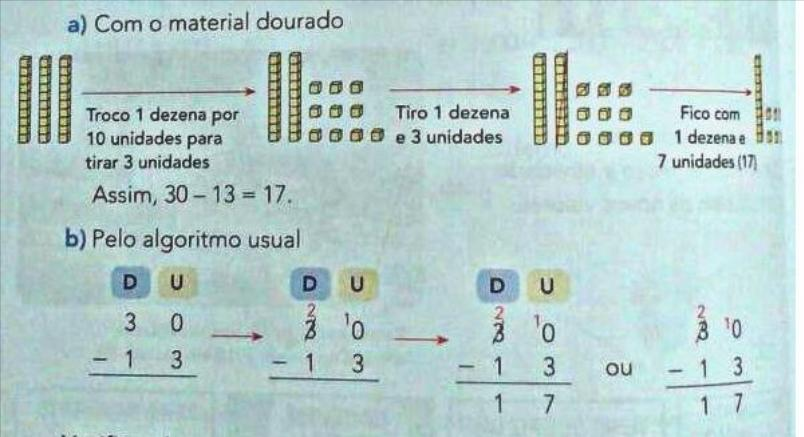
\includegraphics[width=.75\textwidth]{articles/05-material-dourado-com/figura2.jpeg}%
        \caption*{Fonte: \textcite[p.~126]{DANTE2015Projeto}.}%
        \label{fig:dante-subtracao}%
    \end{figure}%

    Assim, o “pegar emprestado” ganha significado para o aluno que passa a entender que há um desagrupamento, uma “transformação” de 1 (um) elemento em 10 (dez), de um grupo abaixo dele. Aqui se utiliza a expressão “fazer troca” ao invés de “pedir emprestado”, pois essa última sugere uma devolução. Quem pediu emprestado tem que devolver.

    \section{Relato da experiência}

    Nesta seção relata-se a experiência de intervenção realizada numa turma do 4º ano --- turno vespertino --- da Escola Estadual Isabel Oscarlina Marques, localizada no município de Santa Cruz/RN cujo objetivo era analisar as contribuições do uso do Material Dourado na compreensão do algoritmo da subtração com reserva.

    A Escola em questão atende cerca de 780 (setecentos e oitenta) alunos do Ensino Fundamental e EJA, distribuídos nos três turnos e conta com 17 (dezessete) funcionários e 30 (trinta) professores graduados na área em que atuam. A estrutura física da escola conta com 10 (dez) salas de aula, quadra esportiva (sem cobertura), secretaria, direção, auditório, sala dos professores, cozinha, refeitório, sala de multimídia, biblioteca e laboratório de informática. Também possui um acervo de materiais didáticos adequados e necessários para o desenvolvimento das aulas, como: televisão, aparelho de som, datashow, notebook, caixas amplificadas, microfones, jogos pedagógicos, entre outros.  

    Quanto aos participantes da pesquisa, foram 14 (catorze) alunos, dos quais 6 (seis) eram do sexo masculino e 8 (oito) do sexo feminino. Todos numa faixa etária entre 10 a 12 anos. 

    Inicialmente, realizou-se reunião com a direção e a coordenação da Escola com o objetivo de apresentar o tema do trabalho: O Material Dourado como recurso didático no ensino do algoritmo da subtração com reserva, bem como pedir permissão para desenvolvê-lo na supracitada instituição. Após, foi apresentada a professora do 4º ano --- vespertino ---, da turma onde seriam realizadas as atividades referentes ao trabalho de pesquisa.  Com ótima acolhida, ela falou sobre a turma nos vários aspectos do ensino-aprendizagem, principalmente no que diz respeito às dificuldades dos alunos no algoritmo da subtração, objeto da pesquisa.  

    Ao se indagar sobre o Material Dourado a professora respondeu que já havia utilizado na sala de aula, mas apenas como demonstração, não realizando nenhuma atividade em que os alunos tivessem a oportunidade de manusear o material. A partir dessas informações percebeu-se que seria viável trabalhar nesta turma o tema em estudo, mediante o perfil traçado preliminarmente pela docente a respeito dos alunos com dificuldades na aprendizagem da subtração com reserva e o fato de a professora não ter utilizado nenhum material manipulável para trabalhar tal conteúdo.  

    De acordo com \textcite{LORENZATO2006Começar}, há uma diferença pedagógica entre uma aula em que o professor apresenta o assunto ilustrando-o com material didático manipulável e uma aula em que os alunos manuseiam o material. Segundo este autor: 

    \begin{quotation}
        O material didático manipulável é o mesmo nas duas situações de ensino, mas os resultados no segundo tipo de aula “serão mais benéficos à formação dos alunos, porque, de posse do material didático manipulável, as observações e reflexões deles são mais profícuas, uma vez que poderão, em ritmos próprios, realizar suas descobertas e, mais facilmente, memorizar os resultados obtidos durante suas atividades \cite[p.~27]{LORENZATO2006Começar}. 
    \end{quotation}

    Dentre os diversos materiais didáticos manipuláveis disponíveis, optou-se pelo Material Dourado por diversos motivos. Primeiramente, porque esse material prioriza a educação sensorial da criança e destina-se a atividades que auxiliam o ensino e a aprendizagem de sistema de numeração decimal-posicional e dos métodos para efetuar as operações fundamentais. Depois, pelas características de material versátil, prático e visual que permite trabalhar a subtração com reserva de uma forma mais fácil de ser entendida e aceita, acreditando-se que: 

    \begin{quotation}
        O trabalho com os materiais concretos torna o processo de construção do sistema numérico mais acessível às crianças, pelas ações que elas realizam sobre eles --- fazer, desfazer grupos, trocar --- do que pelas representações dos elementos. Cada contexto ambiental é um marco na construção do conceito de número, que permite o gradual afastamento dos elementos concretos para a evolução na direção de um sistema mais abstrato e eficiente \cite[p.~65]{GOLBERT1999Matemática}.
    \end{quotation}

    Na verdade, o fator determinante para a escolha do Material dourado foi por ele permitir a composição e decomposição dos numerais para visualizar o processo da subtração com reserva, assim, o “pedir emprestado” passa a ter uma imagem concreta, facilitando, desse modo, a compreensão do aluno sobre o referido processo. 

    Várias são as operações possíveis de serem realizadas com esse recurso, todas elas pressupõem o entendimento anterior das representações e das regras de agrupamentos e desagrupamentos, mas neste trabalho relata-se apenas as atividades relativas à subtração com reserva que é objeto deste estudo.

    \subsection{1º encontro}

    Inicialmente, a professora fez a apresentação da turma, falando sobre o período de atividades de estágio na sala e o propósito da ação. Em seguida, realizou uma atividade de subtração que já estava prevista em seu planejamento. Ela leu um problema do livro didático e resolveu na lousa com ajuda dos alunos, indagando como deveria proceder.  

    Após, aplicou-se a atividade diagnóstica que iria orientar no planejamento de intervenção. Durante a aplicação da atividade observou-se como os alunos resolviam as questões propostas, indagando-os, com a finalidade de verificar que raciocínio eles estavam utilizando para resolver tais questões, no entanto, sem nenhuma interferência na resolução. Recomendou-se, assim, que deveriam resolver as situações-problema utilizando a operação que julgassem correta, ou necessária. Eram quatro questões que traziam problemas envolvendo a subtração com e sem reserva. Percebeu-se claramente que a maioria sentia dificuldade em operar na subtração com reserva, ou seja, quando o minuendo é menor que o subtraendo.  

    A partir dessas constatações adotou-se uma metodologia de trabalho em sala de aula utilizando o Material Dourado como recurso didático para trabalhar com o algoritmo da subtração com reserva.

    \subsection{2º encontro}

    No primeiro momento apresentou-se o Material Dourado, percebendo-se que os alunos já conheciam, pois identificaram cada peça (cubinho, barra, placa e cubo). No entanto, como eles nunca haviam manuseado esse material, reservou-se 20 minutos para brincarem à vontade com ele, fazendo-se construções livres. Pois como afirma Lorenzato:  

    \begin{quotation}
        Ao “ver com as mãos” é mais popular do que geralmente se supõe: você já viu alguém numa loja escolher roupas sem passar as mãos nelas? E crianças em loja de brinquedos conseguem apenas olhá-lo? [\dots] As pessoas precisam “pegar pra ver” como dizem as crianças \cite[p.~18]{LORENZATO2006Começar}.
    \end{quotation}

    \begin{figure}[ht]%
        \centering%
        \caption{Alunos fazendo construções livres com o Material Dourado}%
        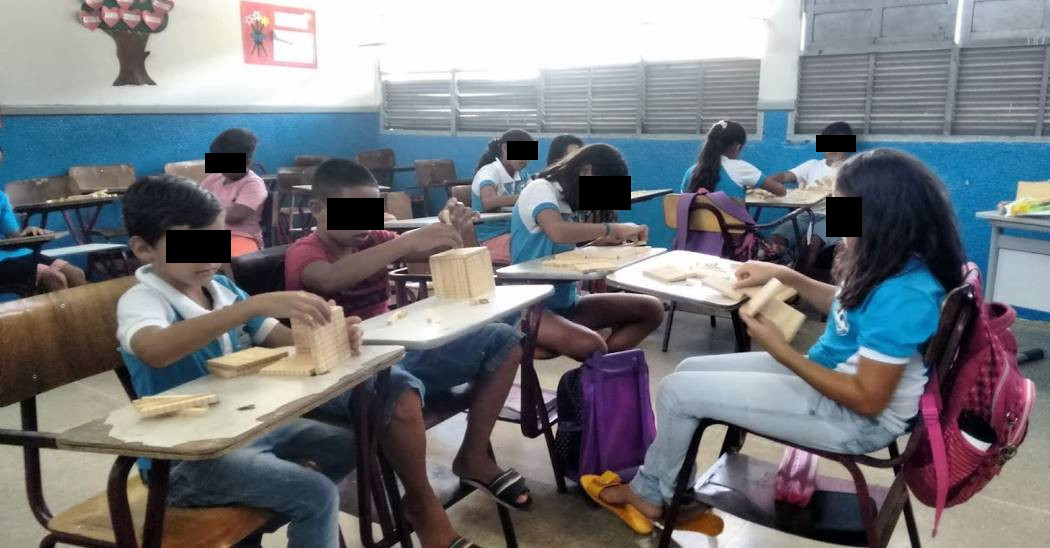
\includegraphics[width=.5\textwidth]{articles/05-material-dourado-com/figura3.jpeg}%
        \caption*{Fonte: Arquivo pessoal.}%
        \label{fig:construcoes-livres-material-dourado}%
    \end{figure}%

    Dienes \cite[apud][p.~34]{TOLEDOAndTOLEDO1997Didática} sugere que “sempre se deve iniciar a construção de um novo conceito a partir da utilização de materiais de apoio”.

    Ainda de acordo com esses autores: 

    \begin{quotation}
        Quando se oferece um material novo para as crianças, a primeira atividade que se recomenda é sempre o jogo livre: apresenta-se o material às crianças e deixa-se que elas utilizem como quiserem [\dots]. A segunda etapa é o jogo com regras, em que se propõe à criança atividades planejadas [\dots]. \cite[p.~72--73]{TOLEDOAndTOLEDO1997Didática}.
    \end{quotation}

    Após o momento de apreciação das construções livres, solicitou-se que fizessem montagens, como: uma barra feita de cubinhos; uma placa feita de barras; um cubo feito de placas, ao mesmo tempo fazendo-se perguntas onde os alunos pudessem estabelecer relações entre as peças. Por exemplo: Quantos cubinhos precisam enfileirar para formar uma barra? Quantas barras são necessárias para formar uma placa? Com quantas placas se forma um cubo?  

    O objetivo era trabalhar primeiro o Sistema de Numeração Decimal (SND), por entender que este é pré-requisito para o bom entendimento do algoritmo da subtração. O propósito era despertar a atenção dos alunos para a percepção de que o cubo é formado por 10 placas, que a placa é formada por 10 barras, e a barra é formada por 10 cubinhos. As crianças participaram ativamente da atividade e a maioria não teve dificuldade para responder os questionamentos. 

    Para finalizar, propôs-se o jogo do Nunca Dez. O objetivo desse jogo também era a compreensão do SND, ou seja, dos agrupamentos de dez em dez (dez unidades formam uma dezena, dez dezenas formam uma centena etc.), característicos do sistema decimal que possibilita fazer agrupamentos de 10 em 10, assim como fazer reagrupamentos, fazer trocas, estimulando o cálculo mental.  

    Para essa atividade formou-se um grande grupo. Cada criança, na sua vez de jogar, lançava o dado e retirava para si a quantidade de cubinhos correspondente à soma dos dois dados. O número que sobressaía no dado dava direito a retirar somente cubinhos. Toda vez que uma criança juntava 10 cubinhos, ela deveria trocar os 10 cubinhos por uma barra. Da mesma maneira, quando tivesse 10 barrinhas poderia trocá-las por uma placa. Previamente foi combinado que o jogo terminaria quando algum aluno conseguisse formar duas placas. 

    \begin{figure}[ht]%
        \centering%
        \caption{Alunos jogando ``Nunca Dez''}%
        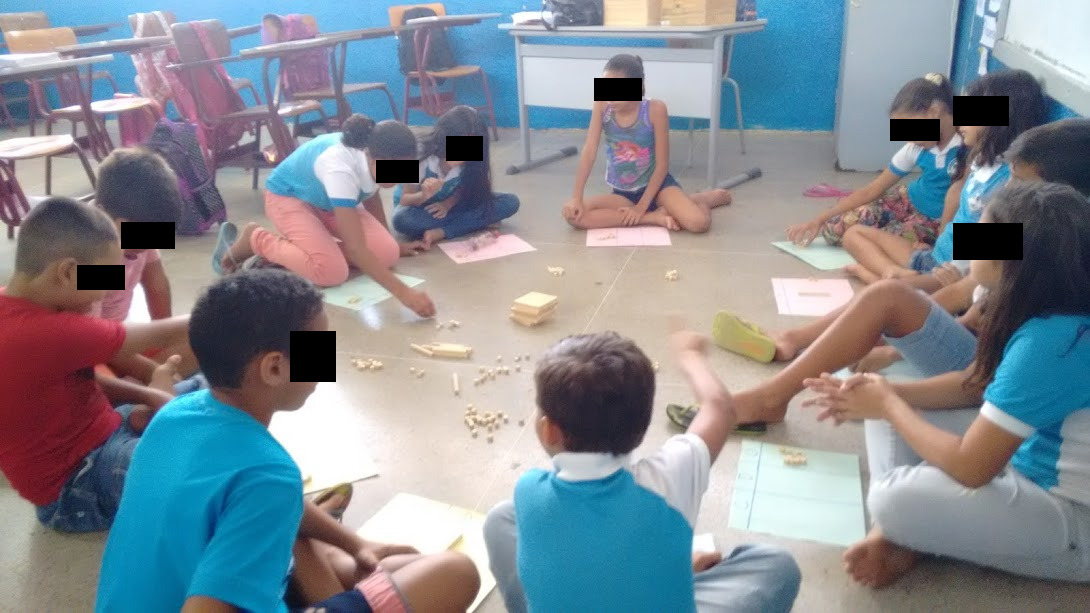
\includegraphics[width=.5\textwidth]{articles/05-material-dourado-com/figura4.jpeg}%
        \caption*{Fonte: Arquivo pessoal.}%
        \label{fig:nunca-dez}%
    \end{figure}%

    Na primeira rodada do jogo, alguns alunos sentiram dificuldade em perceber quando deveriam fazer as trocas, precisando de orientação, mas logo entenderam a dinâmica, e o jogo fluiu satisfatoriamente, constatando-se que a maioria ia fazendo as trocas necessárias. O mais interessante era que ficavam fiscalizando as trocas dos seus colegas. Apenas um aluno precisou de ajuda durante mais tempo. Assim, verificou-se que o Material Dourado facilitou a compreensão do “pedir emprestado” que foi substituído por “fazer trocas”.  

    Centurión afirma que:  

    \begin{quotation}
        Para que os desagrupamentos e trocas possam ser feitos e entendidos pelo aluno no algoritmo da subtração com reserva, é preciso que este aluno tenha compreendido muito bem nosso sistema de numeração posicional de base dez, no qual um algarismo à esquerda de outro vale dez vezes mais do que valeria se ocupasse aquele lugar. É isto que nos permite desagrupar uma centena e transformá-la em dez dezenas; desagrupar uma dezena e trans\-for\-má-la em dez unidades \cite[p.~186]{CENTURIÓN1995Números}.
    \end{quotation}

    Nessa perspectiva, realizou-se um trabalho voltado para o SND, acreditando-se que quando os alunos já conhecem as características da escrita numérica e já estão familiarizados com agrupamentos e trocas na base 10, é possível desenvolver a técnica operatória da subtração com reserva de modo lógico e, portanto, compreensivo.

    \subsection{3º encontro}

    Iniciou-se com a realização de uma atividade denominada “Quanto vou ficar”. Cada aluno após sortear uma ficha teria que representar o número nela contido e, em seguida, realizar a operação de subtração com reserva impressa no verso da ficha, com o auxílio do Material Dourado. O objetivo era perceber as possíveis dificuldades que alguns alunos apresentavam e intervir diretamente a fim de superá-las.  

    Ao final, pediu-se que comentassem o que acharam da atividade. Um aluno falou, entusiasmado: \textit{--- agora compreendo por que estou fazendo as trocas}. Outro respondeu que \textit{``com essas peças fica mais fácil entender por que o 3 virou 13''}.

    \begin{figure}[ht]%
        \centering%
        \caption{Realizando a atividade denominada ``Quanto vou ficar?''}%
        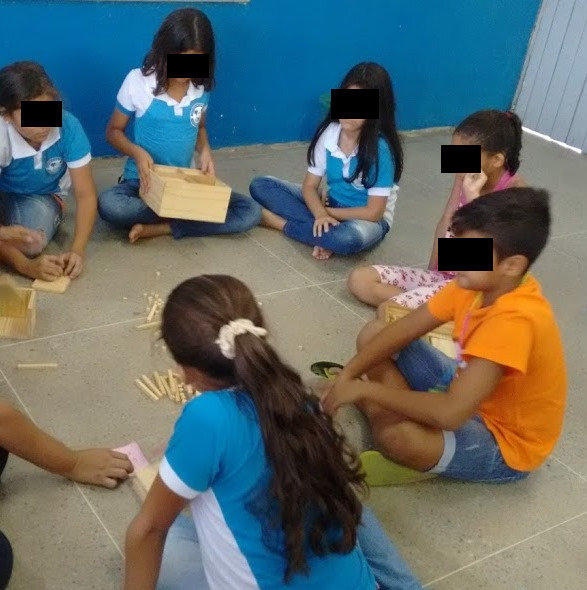
\includegraphics[width=.5\textwidth]{articles/05-material-dourado-com/figura5.jpeg}%
        \caption*{Fonte: Arquivo pessoal.}%
        \label{fig:quanto-vou-ficar}%
    \end{figure}%

    Com essas atividades foi possível perceber que os alunos ao fazerem cálculos com o auxílio do Material Dourado, assimilaram melhor os conceitos básicos presentes na técnica operatória da subtração, como também interagiram com os colegas, trocando ideias e argumentando quando seus resultados divergiam do colega. Assim, consideraram que aprenderam Matemática de forma divertida e prazerosa. 

    Dando continuidade à aula realizou-se uma atividade de subtração xerografada (copiada). Os alunos foram orientados de que deveriam primeiro representar o minuendo com o Material Dourado, em seguida realizar a subtração, e só depois  iriam  anotar  o resultado. À medida que iam realizando as operações os alunos foram solicitados a falar sobre os procedimentos utilizados por eles, sendo mediados nas representações escritas.  

    Percebeu-se que alguns aprenderam mais rapidamente e outros apresentavam algumas dificuldades. Entretanto, foram notórias a concentração dos alunos durante a atividade e a satisfação em estar manuseando o material. Pegavam com muita atenção, tinham cuidado para não perder as peças e quando estavam representando os dados das situações refletiam (trocavam ideias) a cada momento, fixando os olhares nas peças e analisando como realizariam a operação.  

    Desse modo, pode-se concluir que essas atividades favoreceram as crianças a criarem suas próprias estratégias, gerando confiança e autonomia. Assim, diante das peças e utilizando o processo de contagem, realizaram a operação de subtração corretamente, pois podiam ver as barrinhas das dezenas contidas na placa da centena e os cubinhos referentes às unidades, ou melhor, podiam representar com as peças as situações propostas, e mais que isso, visualizar as trocas com material concreto, o que indubitavelmente facilitou a compreensão do processo envolvido na operação.

    \begin{figure}[ht]%
        \centering%
        \caption{Momento da atividade}%
        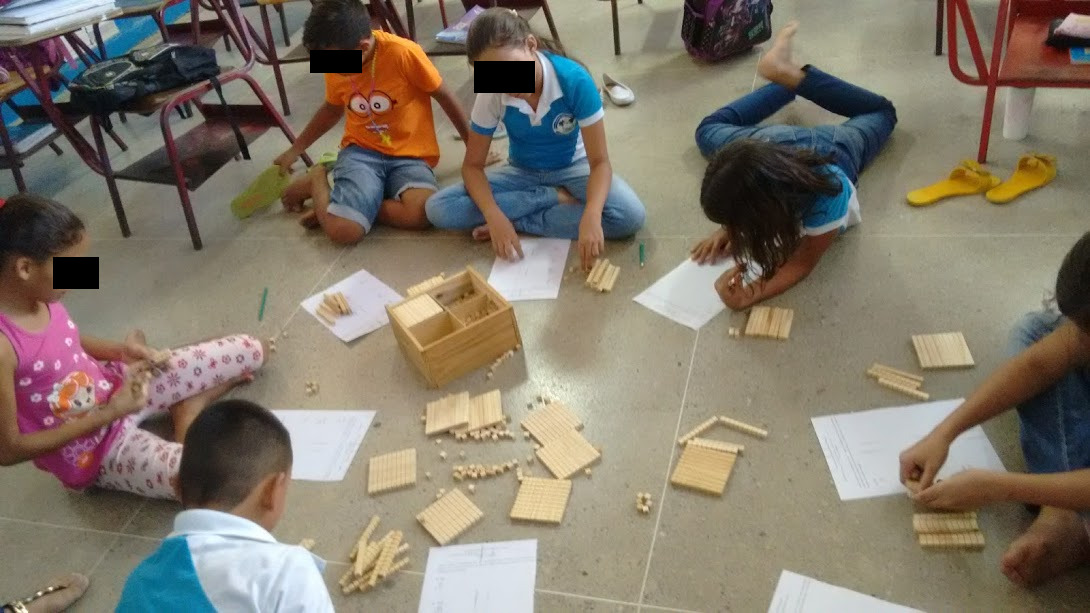
\includegraphics[width=.5\textwidth]{articles/05-material-dourado-com/figura6.jpeg}%
        \caption*{Fonte: Arquivo pessoal.}%
        \label{fig:momento-atividade}%
    \end{figure}%

    \subsection{4º encontro}

    Finalizando os encontros, procederam-se duas atividades: uma individual, trabalhando o algoritmo da subtração com o Material Dourado impresso, a outra, do livro didático do aluno. Em relação à primeira, eles teriam que efetuar “as trocas” através de desenhos. Durante o desenvolvimento dessa atividade observou-se que o Material Dourado ajudou a superar a ideia de que na subtração “pede-se emprestado”, ou seja, o aluno percebeu que, na verdade, não se pede emprestado e sim, realizam-se trocas. O que se faz é decompor uma centena e acrescentar às dezenas, ou decompor uma dezena e acrescentar às unidades, enfim, deve-se entender que há um desagrupamento, uma “transformação” de 1 (um) elemento em 10 (dez) de um grupo de menor valor que ele. 

    \begin{figure}[ht]%
        \centering%
        \caption{Aluna realizando a atividade com material dourado através de desenho}%
        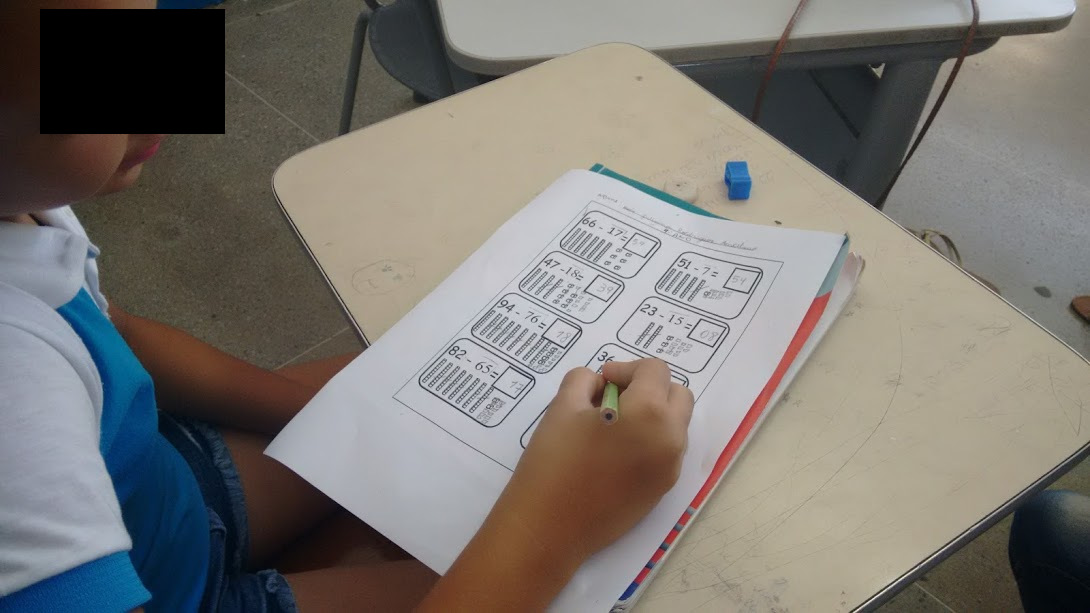
\includegraphics[width=.5\textwidth]{articles/05-material-dourado-com/figura7.jpeg}%
        \caption*{Fonte: Arquivo pessoal.}%
        \label{fig:md-desenho}%
    \end{figure}%

    No que se refere à atividade do livro didático a intenção era verificar se os alunos conseguiam resolver as subtrações com reserva propostas no seu livro. Observou-se que a maioria conseguiu realizar sem auxílio, o que possibilitou concluir que o Material Dourado foi um recurso facilitador nesse processo, pois ajudou aos alunos compreenderem melhor os conteúdos matemáticos trabalhados, propiciando também a interação e a troca de saberes, de maneira que eles tiveram a oportunidade de desenvolver e socializar seus conhecimentos. Sem dúvida, esse material despertou a atenção e o interesse dos alunos envolvidos nesta pesquisa, favorecendo ainda a concentração, além de permitir o contato com o concreto para depois realizar as abstrações pertinentes ao algoritmo da subtração.

    \section{Considerações finais}

    Neste artigo relata-se uma experiência com a utilização do Material Dourado como recurso didático para auxiliar na compreensão do SND e na aprendizagem do algoritmo da subtração com reserva numa turma do 4º ano do Ensino Fundamental. Com essa intervenção, foi possível perceber a evolução cognitiva das crianças envolvidas na pesquisa com relação à aprendizagem da subtração com reserva, pois à medida que se realizavam os trabalhos notava-se, gradativamente, que as dificuldades iam sendo superadas e que aumentava o interesse da turma para realizar as atividades propostas.  

    Essa experiência possibilitou compreender a importância de se trabalhar com metodologias que favorecem aos alunos refletirem sobre as ações realizadas e assim possam construir um saber significativo, desenvolvendo habilidades que lhes permitam passar mais facilmente do concreto para o abstrato. Nessa concepção, propôs-se através do Material Dourado construir o conceito de subtração a partir do concreto, ou seja, o aluno constrói o seu conhecimento, adquirindo base para a abstração; favorecer o questionamento quanto à construção dos conceitos; e quebrar a rotina da aula, propiciando uma maior socialização, interação e interesse da turma.  

    Assim, a aprendizagem se torna mais interessante, pois a partir dessas atividades diferenciadas estimula-se a atenção dos educandos e promove-se também sua autoconfiança. Além disso, a manipulação do concreto faz com que os alunos se sintam agentes de seu próprio conhecimento, uma vez que criam seus métodos e não seguem procedimentos mecânicos e vazios de significado, isto é, sem compreenderem o que estão fazendo. 

    É importante ressaltar que o uso do Material Dourado com o intuito de tornar a aula diferente, alegre, utilizando-o apenas como um recurso motivador, não é suficiente, pois é preciso planejar, definir os objetivos, acreditar que não é uma simples brincadeira, mas sim uma ferramenta importante para um processo de ensino e aprendizagem com qualidade. É fundamental que, paralelamente ao desenvolvimento de atividades, o fazer pedagógico favoreça o pensar matemático, ou seja, os alunos possam reconhecer os conteúdos abordados nas atividades presentes do dia a dia, fazendo as possíveis relações e descobrindo as regularidades existentes.  

    Assim, torna-se imprescindível que a escola implemente projetos visando à melhoria do processo ensino-aprendizagem por meio de ações que priorizem o desenvolvimento integral do aluno e a participação efetiva de todos os envolvidos no processo. Isso só acontecerá se houver uma mudança de atitude, um repensar da prática do professor em prol de uma metodologia que favoreça aos alunos a construção de novos conceitos, sempre apoiados em conceitos já existentes na sua estrutura cognitiva.  

    Dessa forma, conclui-se que o uso do Material Dourado atende a essas expectativas, pois possibilita aos alunos refletirem sobre as ações realizadas, permitindo a construção de um saber significativo com o desenvolvimento de habilidades que propiciam a abstração das construções realizadas, transformando-as em conhecimentos adquiridos efetivamente, atingindo assim o objetivo dessa pesquisa.  

    As experiências no Curso de Especialização em Matemática proporcionaram suportes que subsidiaram na relação entre teoria e prática, apontando os caminhos para que essa pesquisa se desenvolvesse satisfatoriamente. Essa investigação evidencia a necessidade de se trabalhar com metodologias diferenciadas em que os alunos são participantes diretos na construção e significação do conhecimento, bem como destaca a importância da formação continuada do professor para superar as dificuldades que permeiam o ensino de Matemática. Assim, ao término deste trabalho, pode-se afirmar que o uso do Material Dourado no ensino da Matemática, além de facilitar a compreensão do desagrupamento na subtração, dá às relações numéricas abstratas uma imagem mais concreta, facilitando a compreensão e o desenvolvimento do raciocínio lógico, tornando o aprendizado bem mais agradável, pois é dada ao aluno a oportunidade de construir seus conhecimentos de uma forma mais interativa, dinâmica e prazerosa.   

    Conclui-se, então, que a metodologia utilizada nesse trabalho atendeu a expectativa da pesquisadora, atingindo assim o objetivo proposto. Por isso, pode ser utilizada pelos docentes que acreditam numa educação eficaz e prazerosa, capaz de motivar o estudante em prol do seu conhecimento. 

    \nocite{NETO2005Didática}
    \nocite{PANNIZA2006Ensinar}

    \printbibliography[heading=subbibliography,notcategory=fullcited]

    \label{chap:material-douradoend}

\end{refsection}

\begin{refsection}
    \renewcommand{\thefigure}{\arabic{figure}}
    \renewcommand{\thequadro}{\arabic{quadro}}
    
    \chapter[A utilização de modelos e analogias como estratégias de ensino e aprendizagem nas aulas de Química]{\marginpar{
        \begin{flushleft}
            \tiny \sffamily
            Artigo apresentado ao Curso de Pós-graduação do Instituto de Educação Superior Presidente Kennedy (IFESP) para obtenção do título de Especialista em Educação Matemática: teoria e prática no Ensino Fundamental. 
        \end{flushleft}
    }A utilização de modelos e analogias como estratégias de ensino e aprendizagem nas aulas de Química}
    \label{chap:utilizacao-modelos}
    
    \articleAuthor
    {Keila Barbosa da Fonseca}
    {Graduada em Química pela Universidade Federal do Rio Grande do Norte (UFRN). Mestra em Ensino de Ciências e Matemática (UFRN). E-mail: keilafonsec@hotmail.com}
    
    \articleAuthor
    {Lorena Gadelha de Freitas Brito}
    {Bacharela e Licenciada em Química (UFRN), licenciada em Pedagogia (UNINTER), metra em Ensino de Ciências e Matemática (UFRN) atualmente exerço a função de Professora Formadora do Instituto de Educação Superior Presidente Kennedy --- IFESP. ID Lattes: 0725.9511.9576.0694. E-mail: lorenagadelha@yahoo.com.br.}
    
    \begin{galoResumo}
        \marginpar{
            \begin{flushleft}
            \tiny \sffamily
            Como referenciar?\\\fullcite{SelfFonsecaAndBrito2021utilização}\mybibexclude{SelfFonsecaAndBrito2021utilização}, p. \pageref{chap:utilizacao-modelos}--\pageref{chap:utilizacao-modelosend}, \journalPubDate{}
            \end{flushleft}
        }
        Utilizar estratégias de ensino que promovam melhor compreensão de conceitos científicos, pelos alunos, é um desafio para muitos professores de Química da Educação Básica. O estudo do conteúdo, Geometria Molecular, necessário ao entendimento das interações intermoleculares, associado a outros conceitos, muitas vezes, é considerado pelos alunos de difícil compreensão. Nessa perspectiva, o uso de modelos e analogias como estratégias de ensino, podem contribuir com a aprendizagem, proporcionando momentos de reflexão, discussão e participação dos alunos sobre os fenômenos que compõem a natureza. Nesse sentido, a pesquisa tem como objetivo apresentar uma proposta didática sobre Geometria Molecular, utilizando, modelos e analogias com alunos do 1º ano do Ensino Médio da Escola Estadual Professor Edgar Barbosa, localizada na cidade de Natal-RN. Para a coleta de dados, foram utilizados princípios da pesquisa qualitativa e quantitativa e como instrumentos de pesquisa foi utilizado um questionário para avaliar os alunos, sobre o conteúdo proposto durante a unidade. Os resultados apontam que a proposta promoveu além da motivação, uma aprendizagem significativa no processo de ensino e da aprendizagem dos conteúdos abordados, que foi evidenciado através das atividades realizadas, como a criação de modelos concretos que possibilitou um maior envolvimento entre eles.
    \end{galoResumo}
    
    \galoPalavrasChave{Geometria molecular. Modelos. Analogias. Unidades didáticas.}
    
    \begin{otherlanguage}{english}

    \fakeChapterOneLine
    {Use of models and analogies as teaching-learning strategies in Chemistry classes}

    \begin{galoResumo}[Abstract]
        The use of education strategies that promote better understanding of scientific concepts to students can show itself to be quite challenging for many teachers of high schools. The study of the topic “Molecular Geometry”, needed to understand intermolecular relationships, associated with other concepts, is very often considered by the students to be difficult to comprehend. From this perspective, the use of models and analogies as teaching strategies can contribute to the learning, giving the students the opportunity to reflect and discuss natural phenomena. In this sense, the research has as an objective to present a didactic alternative to students taking the second year of high school at Escola Estadual Professor Edgar Barbosa, in Natal, Rio Grande do Norte, Brazil. Qualitative and quantitative research principles were used to collect data in a survey answered by the students. The replies show that the activities promoted significant improvement in students' learning, motivation and engagement.
    \end{galoResumo}
    
    \galoPalavrasChave[Keywords]{Molecular Geometry. Models. Analogies. Teaching Units.}
    \end{otherlanguage}

    \section{Introdução}

    No Ensino de Química, o grande número de conceitos abstratos, torna a disciplina bastante complexa e de difícil compreensão de uma série de fenômenos da natureza, despertando no professor a necessidade de utilizar novas ferramentas que possam contribuir para o entendimento dos alunos sobre diferentes conceitos. Nesse sentido, o uso de modelos e analogias, configura como um importante recurso/estratégia no processo de ensino e da aprendizagem dessa ciência e com essa abordagem, pode despertar um maior interesse dos alunos pela disciplina.  

    No meio educacional, discussões apontam para uma concepção diferenciada do conhecimento científico, sendo esse, relacionado com uma tentativa de compreensão e explicação de fenômenos do mundo natural. O desenvolvimento desse tipo de conhecimento utiliza constantemente representações que apresentam um caráter provisório, e são chamadas de modelos. De acordo com \textcite{GALAGOVSKYAndADÚRIZBRAVO2001Modelos}, os modelos são considerados ferramentas de representação teórica do mundo, auxiliando a sua explicação, predição e transformação. 

    Para este trabalho, foi abordado conceitos químicos relacionados a Geometria Molecular e polaridade das moléculas no 1º ano do Ensino Médio. Para desenvolver o estudo foi utilizado aulas expositivas e dialogadas, experimentais, modelos e analogias para explicar e fazer a mediação entre o conhecimento que o aluno já possui e os novos conceitos científicos que serão abordados neste artigo, buscando investigar, desse modo as possíveis potencialidades que essas ferramentas de ensino podem trazer para as aulas de Química.

    \section{Modelos e analogias no ensino de química e a aprendizagem significativa}

    O desenvolvimento de atividades baseadas na utilização de modelos, pode contribuir para a reflexão, discussão e participação dos alunos em sala de aula. A construção do conhecimento é favorecida, não somente pela apresentação dos modelos aos alunos, mas também pelo desenvolvimento de atividades que priorizem a construção de modelos representacionais, permitindo ao aluno utilizar os conhecimentos escolares em outras situações do seu cotidiano. Nessa perspectiva, a participação do professor durante esse processo é fundamental para criar possibilidades de produzi-lo e explorá-lo, contribuindo para uma melhor compreensão dos alunos de forma que esse recurso possa contribuir para a construção do conhecimento. 

    Consideradas importantes ferramentas no processo educativo, as analogias conferem poder discursivo ao conhecimento científico, dando uma nova visão do não observável, providenciando formas de argumentação. Nessa perspectiva, a Teoria da Aprendizagem Significativa (TAS) de David Ausubel, pode ajudar a reestruturar a memória já existente e prepará-la para novas informações.  

    De acordo com essa teoria, a nova informação interage em comum, à estrutura de conhecimento específico, chamada pelo autor de conceito \textit{subsunçor}. Quando o conteúdo escolar a ser aprendido não consegue ligar-se a algo já conhecido, ocorre uma aprendizagem mecânica, ou seja, as informações são aprendidas sem interagir com conceitos relevantes existentes na estrutura cognitiva. Assim, a pessoa decora fórmulas, leis, mas esquece após uma avaliação. Para haver aprendizagem significativa são necessárias duas condições. Em primeiro lugar, o aluno precisa ter uma disposição para aprender: se o indivíduo quiser memorizar o conteúdo arbitrária e literalmente, então a aprendizagem será mecânica. Em segundo, o conteúdo escolar a ser aprendido tem que ser potencialmente significativo \cite{AUSUBEL2000The}. 

    A utilização de recursos que facilitem a aquisição do conhecimento de forma significativa, por exemplo, uso de modelos e analogias, deve levar em conta a existência de subsunçores na estrutura cognitiva do aluno. Caso o novo conteúdo não encontre âncoras, podem ser utilizados conteúdos introdutórios com o objetivo de preencher a lacuna existente entre o que se sabe e o que se deseja que o aluno aprenda. Sobre a utilização de analogias, pode-se compreender que desempenham um papel importante na construção de um novo modelo que ultrapassa a dimensão do que é observável, contribuindo para a construção de um conhecimento novo \cite{MORTIMER2000Linguagem}.

    Para evitar o surgimento de concepções alternativas nos estudantes, o professor deve compreender que sua aplicação não é tão óbvia como muitos pensam, e para utilizá-las deve fazer uso do Modelo de Ensino com Analogias \textit{Teachinhg Wiht Analogies} (TWA), apresentado por \textcite{HARRISONAndTREAGUST1993Teaching}. 

    De acordo com Harrison e Treagust, a utilização desses modelos envolvem as seguintes etapas:

    \begin{quotation}
        Introdução do conceito alvo a ser aprendido, por meio de uma breve ou completa explicação de acordo com a analogia a ser empregada; Sugerir a situação análoga aos alunos e mediante discussões estimar a familiaridade dos estudantes com o análogo; Identificar as características relevantes do análogo; Mapear as similaridades entre alvo e análogo; Indicar onde a analogia falha, onde o análogo e o alvo não têm correspondência; Esboçar conclusões sobre o alvo \cite[p.~1291]{HARRISONAndTREAGUST1993Teaching}. 
    \end{quotation}

    Assim, a sequência dos passos propostos pelo Modelo TWA pode ser modificada segundo \textcite{HARRISONAndTREAGUST1993Teaching}, sofrendo influências de alguns fatores, tais como: estilo do professor; particularidades do conceito científico e o análogo que está sendo estudado, estimulando alunos a elaborar analogias, tendo em vista que o desenvolvimento dessa atividade pode contribuir para explicar e compreender não somente o conteúdo Geometria Molecular, mas diversos conteúdos presentes no Ensino da Química. 

    \section{Vantagens e desvantagens do trabalho com modelos e analogias}

    A palavra modelo pode apresentar diferentes significados, tais como: tipo de objeto, padrão a seguir, exemplo de perfeição, representação concreta de um objeto capaz de reproduzir suas principais características visuais e estruturais, dentre outros. Em um contexto científico, \textcite{GILBERT2004Models} considera que um modelo é a representação parcial de um objeto, um evento, um processo ou uma ideia, criado com objetivo específico. Nesse sentido, os modelos, criações da mente humana, são representações que apresentam contribuições no ensino de ciências desempenhando vários objetivos, tais como: simplificar entidades complexas, contribuir com a comunicação de ideias, favorecer a visualização de entidades abstratas e fundamentar a proposição e a interpretação de experimentos sobre a realidade. 

    \textcite{DUARTE2005Analogias} em seu trabalho apresenta algumas potencialidades sobre o uso de analogias que ativam o raciocínio analógico, organizam a percepção, desenvolvem capacidades cognitivas como a criatividade e a tomada de decisão, que tornam o conhecimento científico mais inteligível e plausível, facilitando a compreensão, a visualização de conceitos abstratos, podendo promover o interesse dos alunos e podem ser utilizadas para avaliar o conhecimento e a compreensão dos alunos.  

    Algumas dificuldades podem ocorrer a partir dessas analogias, como: a analogia pode ser interpretada como o conceito em estudo, ou dela serem apenas retidos os detalhes mais evidentes e apelativos, sem se chegar a atingir o que se pretendia; podem não ocorrer um raciocínio analógico que leve a compreensão da analogia; a analogia pode não ser reconhecida como tal, não ficando explícita a sua utilidade; os alunos podem centrar-se nos aspectos positivos da analogia e desvalorizar as suas limitações. Dessa forma, compreende-se que a compreensão dos conceitos científicos na Química e em outras ciências que depende do domínio de uma série de habilidades como raciocínio abstrato, domínio da linguagem simbólica, podem ser favorecidos pelo uso dessa estratégia de ensino. 

    \section{Elaboração de uma sequência didática}

    Uma unidade didática ou sequência didática é um trabalho que compreende a escolha de estratégias de ensino que contribuam para a construção de um conhecimento mais significativo \cite{CAAMAÑO2011Enseñar}.

    Segundo \textcite{ZABALA1998prática} sequência didática é um encadeamento de passos ou etapas ligadas entre si, para tornar mais eficiente o processo de aprendizagens planejadas e desenvolvidas com objetivos educacionais específicos com início, meio e fim conhecido tanto por professores quanto por alunos. Nessa perspectiva, é fundamental o envolvimento de todos, cabendo ao professor o papel de mediador durante a ação de construção do conhecimento e necessitando dos alunos a disponibilidade e o interesse de aprender. A estruturação da aula a partir de uma Unidade didática favorece a criatividade, a flexibilidade e inovação, fatores que podem contribuir com o desenvolvimento da autonomia do aluno. Nesse sentido pode-se dizer que o aluno tem a oportunidade de \textit{aprender a aprender}.  

    O desenvolvimento de uma unidade didática é um processo complexo, que pode tomar vários caminhos e envolve em seu planejamento, tomada de decisão que implica na escolha dos objetivos, seleção e organização dos conteúdos, sequências de atividades, seleção de atividades de avaliação, organização e gestão da aula.  

    \section{Procedimentos metodológicos}

    A pesquisa se enquadra em uma perspectiva qualitativa e quantitativa, baseada na pesquisa-ação que envolve a análise de dados escritos, ações e comunicações dos participantes reunidos através da utilização de instrumentos de coletas de dados. De acordo com \textcite{FLICK2009Introdução} a pesquisa qualitativa considera as observações realizadas no cotidiano e no contexto social como importantes para investigação. Caracterizada como uma pesquisa-ação em que o pesquisador e participantes estão envolvidos de modo cooperativo e participativo.  

    O público-alvo da pesquisa foram trinta e nove alunos do Ensino Médio da Escola Estadual Professor Edgar Barbosa localizada no Município do Natal/RN. Para investigar as concepções dos alunos sobre os modelos, foi aplicado, um questionário e os resultados obtidos foram organizados em gráficos e quadros. 

    \section{Resultados e discussões}

    A sequência didática elaborada foi aplicada em 3 encontros, totalizando 6 aulas de cinquenta minutos cada. Foram abordados os conteúdos envolvendo Geometria Molecular e interações intermoleculares. As atividades realizadas e os recursos utilizados em cada encontro serão descritos a seguir. 

    Com o objetivo de levantar as concepções prévias acerca do termo \textit{modelo} e sua utilização nas aulas de Química, inicialmente foi aplicado com 39 alunos identificados como A1 a A39 um questionário sobre o tema, envolvendo os diferentes significados que o termo \textit{modelo} pode assumir na Língua Portuguesa. Algumas ideias expressadas pelos alunos, merecem destaque e serão apresentadas a seguir: \textit{Modelo seria uma representação de algo como modelo de revistas que representa marcas de roupas ou modelo de Thomson que representa sua forma de ver o átomo} (A27). \textit{Tipo um exemplo, algo a ser seguido, que serve para visualizar e aprender. É importante sim, aprendo mais com ele} (A32). \textit{Modelo é um exemplo aproximado de algo. Ex: Modelo das fitas de DNA} (A11).  

    Após o levantamento das ideias prévias dos alunos participantes da pesquisa, imagens relacionadas aos diferentes significados da palavra foram apresentadas por meio de slides que representavam os diferentes significados que o termo modelo pode assumir e suas características. 

    Em seguida foi trabalhado com os alunos o conteúdo de Ligações Químicas, que de acordo com \textcite{FERNANDEZAndMARCONDES2006Concepções} os conceitos abordados sobre Ligações Químicas, estão bem relacionados com a constituição da matéria, ou seja, conceitos abstratos e, consequentemente, demandam dos alunos um desenvolvimento cognitivo mais próximo do lógico-formal, um pensamento abstrato mais organizado. Dessa forma, com o propósito de favorecer uma compreensão mais adequada do assunto foram utilizadas estratégias como apresentação de um vídeo sobre: condutividade elétrica dos materiais, e atividades de modelagem.  

    Inicialmente, os alunos assistiram o vídeo e em seguida, após a apresentação foi realizado a seguinte questionamento: Por que o cloreto de sódio conduziu corrente elétrica quando em solução aquosa e não conduziu corrente no estado sólido? As concepções iniciais dos alunos podem ser vistas a seguir: \textit{É que a água é um condutor, mas mostra que a água não conduz} (A32). \textit{Modificou a estrutura do sólido, nesse caso está mais comprimido como se estivesse de uma forma e quando colocou na água formou um novo tipo que conduziu} (A3). \textit{Eu acho que mudou o estado físico, como se tivesse aberto espaço} (A22).

    De acordo com \textcite{MACHADOAndMORTIMER2007Química} o conhecimento químico é construído pela combinação de três níveis representacionais: fenomenológico, teórico e representacional, o que pode ser traduzido para realização de uma discussão nas dimensões: macroscópica, submicroscópica e simbólica. De acordo com \textcite{MORAIS2007Recurso} a utilização de modelos para intermediar o aprendizado, é simples e ajuda os alunos a desenvolver a percepção do arranjo espacial das ligações químicas existentes entre os núcleos atômicos que compõem uma molécula. O quadro 1 mostra os resultados das estruturas criadas pelos alunos com diferentes materiais para representar diferentes moléculas.

    \begin{longquadro}[t]{ | c m{.26\textwidth} c c |}
    
        \caption{Estruturas criadas pelos alunos e materiais utilizados na atividade proposta}
        \label{quad:estruturas-quimicas}\\
       
        \hline
        Estruturas criadas & Materiais utilizados & Geometria & Nomenclatura\\
        \hline
        \endfirsthead

        \multicolumn{4}{c}{\footnotesize \textsf{Quadro \ref{quad:estruturas-quimicas}~--~\textit{Estruturas criadas pelos alunos e materiais utilizados na at\dots (continuação)}}\medskip }\\
        \hline
        Estruturas criadas & Materiais utilizados & Geometria & Nomenclatura\\
        \hline
        \endhead

        \multicolumn{4}{r}{\footnotesize \textsf{\textit{continua}}}\\
        \endfoot
       
        \hline
        \caption*{Fonte: elaboração da autora}
        \endlastfoot

        \makecell{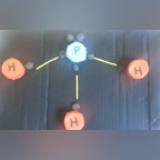
\includegraphics[width=0.20\textwidth]{articles/06-utilizacao-de-modelo/quadro1-1.jpeg}}%
            & \begin{itemize}[series=nospace,nosep,leftmargin=*,after=\vspace{-\baselineskip},before=\vspace{-\baselineskip}]%
                \item Tampas de garrafa%
                \item Palitos de madeira%
                \item Lã de aço%
                \item Papelão%
                \item Tinta%
            \end{itemize} %%
            & \makecell{Piramidal} %
            & \makecell{\ce{PH3}\\(Hidreto de fósforo)} \\

        \hline

        \makecell{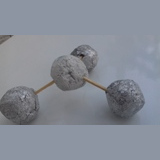
\includegraphics[width=0.20\textwidth]{articles/06-utilizacao-de-modelo/quadro1-2.jpeg}}%
            & \begin{itemize}[series=nospace,nosep,leftmargin=*,after=\vspace{-\baselineskip},before=\vspace{-\baselineskip}]%
                \item Folha de alumínio%
                \item Palitos de madeira%
            \end{itemize} %%
            & \makecell{Piramidal} %
            & \makecell{\ce{NH3}\\(Amônia)}\\

        \hline

        \makecell{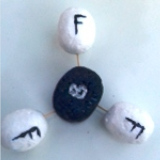
\includegraphics[width=0.20\textwidth]{articles/06-utilizacao-de-modelo/quadro1-3.jpeg}}%
            & \begin{itemize}[series=nospace,nosep,leftmargin=*,after=\vspace{-\baselineskip},before=\vspace{-\baselineskip}]
                \item Bolinhas de isopor
                \item Palitos de madeira
                \item Tinta
            \end{itemize} %%
            & \makecell{Trigonal\\plana} %
            & \makecell{\ce{BF3}\\(Trifluoreto de boro)} \\

        \hline

        \makecell{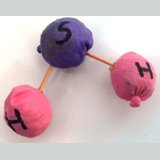
\includegraphics[width=0.20\textwidth]{articles/06-utilizacao-de-modelo/quadro1-4.jpeg}}%
            & \begin{itemize}[series=nospace,nosep,leftmargin=*,after=\vspace{-\baselineskip},before=\vspace{-\baselineskip}]
                \item Bexiga de ar
                \item Arroz
                \item Caneta colorida
                \item Palito de madeira
            \end{itemize} %%
            & \makecell{Angular} %
            & \makecell{\ce{H2S}\\(Ácido sulfídrico)} \\

        \hline

        \makecell{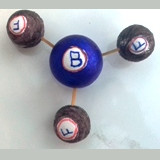
\includegraphics[width=0.20\textwidth]{articles/06-utilizacao-de-modelo/quadro1-5.jpeg}}%
            & \begin{itemize}[series=nospace,nosep,leftmargin=*,after=\vspace{-\baselineskip},before=\vspace{-\baselineskip}]
                \item Bolinhas de isopor
                \item Palitos de madeira
                \item Tinta
            \end{itemize} %%
            & \makecell{Trigonal\\plana} %
            & \makecell{\ce{BF3}\\(Trifluoreto de boro)} \\

        \hline

        \makecell{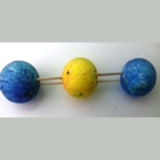
\includegraphics[width=0.20\textwidth]{articles/06-utilizacao-de-modelo/quadro1-6.jpeg}}%
            & \begin{itemize}[series=nospace,nosep,leftmargin=*,after=\vspace{-\baselineskip},before=\vspace{-\baselineskip}]
                \item Bolinhas de isopor
                \item Palitos de madeira
                \item Tinta
            \end{itemize} %%
            & \makecell{Linear} %
            & \makecell{\ce{CO2}\\(Gás carbônico)} \\

        \hline

        \makecell{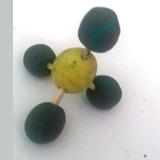
\includegraphics[width=0.20\textwidth]{articles/06-utilizacao-de-modelo/quadro1-7.jpeg}}%
            & \begin{itemize}[series=nospace,nosep,leftmargin=*,after=\vspace{-\baselineskip},before=\vspace{-\baselineskip}]%
                \item Massa de modelar%
                \item Palitos de madeira%
            \end{itemize} %%
            & \makecell{Tetraédrica} %
            & \makecell{\ce{CH4}\\(Gás metano)} \\

        \hline

        \makecell{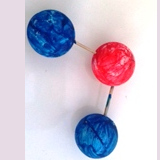
\includegraphics[width=0.20\textwidth]{articles/06-utilizacao-de-modelo/quadro1-8.jpeg}}%
            & \begin{itemize}[series=nospace,nosep,leftmargin=*,after=\vspace{-\baselineskip},before=\vspace{-\baselineskip}]
                \item Bolinhas de isopor
                \item Palitos de madeira
                \item Tinta
            \end{itemize} %%
            & \makecell{Angular} %
            & \makecell{\ce{H2O}\\(Água)} \\

        \hline

        \makecell{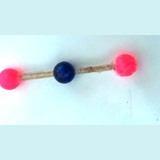
\includegraphics[width=0.20\textwidth]{articles/06-utilizacao-de-modelo/quadro1-9.jpeg}}%
            & \begin{itemize}[series=nospace,nosep,leftmargin=*,after=\vspace{-\baselineskip},before=\vspace{-\baselineskip}]
                \item Miçangas
                \item Palitos de madeira
                \item Fita adesiva
            \end{itemize} %%
            & \makecell{Linear} %
            & \makecell{\ce{CO2}\\(Gás carbônico)} \\
    \end{longquadro}

    Através dos modelos elaborados, foi observado que os grupos utilizaram os mais diversos materiais em suas produções e a maioria deles expressou de forma coerente as ligações existentes entre os átomos. Apenas dois grupos apresentaram dificuldades em representar de forma correta o arranjo espacial. Nesse sentido, a confecção dos modelos contribuiu para o processo de formação conceitual sobre a disposição dos átomos na representação de uma molécula, tendo em vista que a partir de uma estratégia como essa foi possível perceber que os alunos visualizassem as estruturas de forma tridimensional. Após a apresentação dos modelos, os alunos preencheram uma tabela no caderno representando os modelos construídos e suas respectivas geometrias.  

    No encontro seguinte foi abordado o conceito de solubilidade, já que a partir dele é possível compreender outros conceitos químicos, como as interações existentes entre as moléculas das substâncias. Nesse sentido, foi realizado um experimento envolvendo diferentes substâncias e a partir dos resultados obtidos com a atividade experimental os alunos, responderam as seguintes questões: 

    \begin{enumerate}
        \item Os materiais moleculares apresentam o mesmo comportamento com relação à dissolução? 
        \item Quais as substâncias ou produtos comerciais (água, óleo de soja, vaselina ou parafina e vinagre) têm comportamento semelhante ao do sal de cozinha? 
        \item Ocorre ou não dissolução entre materiais moleculares? Que conclusões você pode extrair desse experimento?
    \end{enumerate}

    Os resultados obtidos com os questionamentos podem ser observados nos gráficos das Figuras \ref{fig:resp-q1-quim}, \ref{fig:resp-q2-quim} e \ref{fig:resp-q3-quim}.
    
    \begin{figure}[ht]%
        \centering%
        \caption{Respostas dos alunos à Questão 1}%
        \begin{tikzpicture}
            \pie[text=legend, radius=2]{74/Comportamento distinto,
                12/Comportamento semelhante,
                14/Não responderam}
        \end{tikzpicture}
        \caption*{Fonte: Elaborado pela autora.}%
        \label{fig:resp-q1-quim}%
    \end{figure}%

    \begin{figure}[ht]%
        \centering%
        \caption{Respostas dos alunos à Questão 2}%
        \begin{tikzpicture}
            \pie[text=legend, radius=2]{54/Água e vinagre,
                26/Somente o vinagre,
                3/Todas,
                17/Não responderam}
        \end{tikzpicture}
        \caption*{Fonte: Elaborado pela autora.}%
        \label{fig:resp-q2-quim}%
    \end{figure}%

    \begin{figure}[ht]%
        \centering%
        \caption{Respostas dos alunos à Questão 3}%
        \begin{tikzpicture}
            \pie[text=legend, radius=2]{49/Depende da polaridade,
                23/Ocorre,
                17/Não ocorre,
                11/Não responderam}
        \end{tikzpicture}
        \caption*{Fonte: Elaborado pela autora.}%
        \label{fig:resp-q3-quim}%
    \end{figure}%

    Na sequência construíram modelos concretos utilizando materiais alternativos para representar as interações existentes entre as substâncias, o resultado do trabalho realizado por eles, pode ser visto no Quadro \ref{quad:modelos-quimicos}.

    Na elaboração dos modelos, os alunos utilizaram os mais diversos materiais, desde papel cortado em tiras até flocos de arroz tingidos. De acordo com \textcite{JUSTI2006enseñanza} a aprendizagem por meio de modelos pode ter lugar em dois momentos do processo: na construção (modelagem) e na utilização do modelo, visto que quando um modelo é construído, cria-se um tipo de estrutura representativa, desenvolvendo, assim, uma forma científica de pensar, bem como também, aprende-se sobre a situação representada.

    \begin{longquadro}[t]{ | c m{.30\textwidth} c |}
    
        \caption{Modelos criadas pelos alunos}
        \label{quad:modelos-quimicos}\\
       
        \hline
        Modelos criadas & Material utilizado & Sistemas representados\\
        \hline
        \endfirsthead

        \multicolumn{3}{c}{\footnotesize \textsf{Quadro \ref{quad:modelos-quimicos}~--~\textit{Modelos criadas pelos alunos (continuação)}}\medskip }\\
        \hline
        Modelos criadas & Material utilizado & Sistemas representados\\
        \hline
        \endhead

        \multicolumn{3}{r}{\footnotesize \textsf{\textit{continua}}}\\
        \endfoot
       
        \hline
        \caption*{Fonte: elaboração da autora}
        \endlastfoot

        \makecell{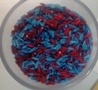
\includegraphics[width=0.20\textwidth]{articles/06-utilizacao-de-modelo/quadro2-1.jpeg}}%
            & Arroz tingido nas cores azul e vermelho%
            & \makecell{Mistura homogênea}\\
        \hline

        \makecell{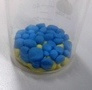
\includegraphics[width=0.20\textwidth]{articles/06-utilizacao-de-modelo/quadro2-2.jpeg}}%
            & Massa de modelar nas cores azul e amarelo%
            & \makecell{Mistura heterogênea}\\
        \hline

        \makecell{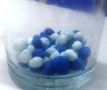
\includegraphics[width=0.20\textwidth]{articles/06-utilizacao-de-modelo/quadro2-3.jpeg}}%
            & Massa de modelar nas cores azul e branco%
            & \makecell{Mistura homogênea}\\
        \hline

        \makecell{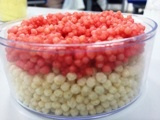
\includegraphics[width=0.20\textwidth]{articles/06-utilizacao-de-modelo/quadro2-4.jpeg}}%
            & Flocos de arroz nas cores vermelho e amarelo%
            & \makecell{Mistura heterogênea}\\

        \hline

        \makecell{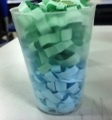
\includegraphics[width=0.20\textwidth]{articles/06-utilizacao-de-modelo/quadro2-5.jpeg}}%
            & Tiras de papel nas cores azul e verde%
            & \makecell{Mistura heterogênea}\\

        \hline

        \makecell{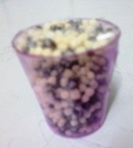
\includegraphics[width=0.20\textwidth]{articles/06-utilizacao-de-modelo/quadro2-6.jpeg}}%
            & Cereais de chocolate ao leite e chocolate branco%
            & \makecell{Mistura homogênea}\\

        \hline

        \makecell{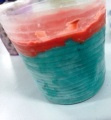
\includegraphics[width=0.20\textwidth]{articles/06-utilizacao-de-modelo/quadro2-7.jpeg}}%
            & Massa de modelar nas cores laranja e verde%
            & \makecell{Mistura heterogênea}\\

        \hline

        \makecell{\includegraphics[width=0.20\textwidth]{articles/06-utilizacao-de-modelo/quadro2-8.jpeg}}%
            & Flocos de isopor nas cores azul e branco%
            & \makecell{Mistura heterogênea}\\

    \end{longquadro}

    \section{Considerações finais}

    Através das estratégias e recursos utilizados na elaboração das atividades, foi observado que a maioria dos alunos envolvidos conseguiram desenvolver uma boa compreensão dos conceitos abordados nessa proposta de ensino  

    A sequência didática para o Ensino de Química foi bem aceita pelos alunos, possibilitando a interação e a socialização das ideias, motivando-os e despertando o interesse dos diversos conteúdos abordados nas aulas, elementos que foram importantes para a construção do conhecimento em sala de aula.  

    Portanto, diante do que foi exposto, se faz necessário uma reflexão pelos professores de Química sobre a utilização de estratégias de ensino, como o uso de modelos e analogias durante as aulas, e as contribuições que a utilização dessas estratégias pode trazer ao processo de ensino e aprendizagem da Química no Ensino Médio.  

    \nocite{NOVAK1991Ayudar}
    \nocite{NUNESAndFERRAZDAndJUSTINA2007Estudos}

    \printbibliography[heading=subbibliography,notcategory=fullcited]

    \label{chap:utilizacao-modelosend}

\end{refsection}

\begin{refsection}
    \renewcommand{\thefigure}{\arabic{figure}}
    
    \chapterOneLine
    {Uma reflexão diante do pedagogo empresarial como gestor da ouvidoria }
    \label{chap:reflexao-pedagogo}

    \articleAuthor
    {Tâmara Maria Soares de Medeiros de Cavalcanti}
    {Graduada em Pedagogia pelo Instituto de Educação Superior Presidente Kennedy (IFESP). Especialista em Gestão em Processos Educacionais. E-mail: tmsoares@globo.com.}
    
    \articleAuthor
    {Ilsa Fernandes de Queiroz}
    {Graduada em Ciências Sociais (UFRN). Mestra em Ciências Sociais (UFRN). Professora Formadora do IFESP. ID Lattes: 6966.1039.5536.5909. E-mail: ilsafe13@yahoo.com.br.}
    
    \begin{galoResumo}
        \marginpar{
            \begin{flushleft}
            \tiny \sffamily
            Como referenciar?\\\fullcite{SelfCavalcanteAndQueirozAndesde2021Uma}\mybibexclude{SelfCavalcanteAndQueirozAndesde2021Uma}, p. \pageref{chap:reflexao-pedagogo}--\pageref{chap:reflexao-pedagogoend}, \journalPubDate{}
            \end{flushleft}
        }
        O Presente estudo pretende evidenciar a atuação do Pedagogo em um ambiente empresarial na gestão da Ouvidoria de uma Instituição Financeira Pública. Apresenta uma pesquisa bibliográfica além de uma pesquisa de campo por meio de uma rigorosa observação nos canais de comunicação da ouvidoria dentre eles: o Fale Conosco, o telefone 0800 e o e-mail. Nesse sentido, a pesquisa aponta a importância da presença do pedagogo na ouvidoria, contribuindo para um trabalho mais humanizado, com possibilidades de análises mais seguras, buscando colocar à disposição do cidadão um serviço de qualidade. No primeiro item, apresenta-se o que é a empresa ouvidoria, de que forma se apresenta do ponto de vista econômico, tendo o Governo do RN como sócio majoritário. No segundo, detém-se no foco do trabalho do Pedagogo como especialista em aprendizagem e Educação. No terceiro, o pedagogo como líder que recebe, analisa e oferece respostas conclusivas, após eventual encaminhamento para instrução junto aos setores responsáveis. No quarto, compreende-se a presença do pedagogo de grande relevância para fortalecer práticas de acolhimento dos cidadãos fomentando convivências geradoras de exercícios mais democráticos. 
    \end{galoResumo}
    
    \galoPalavrasChave{Pedagogia. Ouvidor. Gestão.}
    
    \begin{otherlanguage}{english}

    \fakeChapterOneLine
    {A reflection before business educators as a manager of the ombudsman}

    \begin{galoResumo}[Abstract]
        This study intends to highlight the role of the Pedagogue in a business environment in the management of the Ombudsman of a Public Financial Institution. It presents bibliographical research in addition to a field research through a rigorous observation of the ombudsman's communication channels, among them: Fale Conosco, the 0800 telephone and the e-mail. In this sense, the research points out the importance of the presence of the pedagogue in the ombudsman, contributing to a more humanized work, with safer analysis possibilities, seeking to make a quality service available to the citizen. The first item presents what the ombudsman company is, how it presents itself from the economic point of view, with the Government of RN as the majority partner. In the second, it focuses on the work of the Pedagogue as a specialist in learning and education. In the third, the pedagogue as a leader who receives, analyzes and offers conclusive answers, after an eventual referral for instruction with the responsible sectors. In the fourth, it is understood the presence of a highly relevant pedagogue to strengthen citizen welcoming practices, fostering interactions that generate more democratic exercises. 
    \end{galoResumo}
    
    \galoPalavrasChave[Keywords]{Pedagogy. Ombudsman. Management.}
    \end{otherlanguage}


    \section{Introdução}

    O estudo descreve sobre a pesquisa do Curso de Especialização em Gestão de Processos Educacionais, do Instituto de Educação Superior Presidente Kennedy. Busca relatar a atuação do Pedagogo em ambiente empresarial na gestão da Ouvidoria de uma Instituição Financeira Pública.  

    A Empresa é a associação de pessoas, explorando uma atividade com objetivo definido, liderada pelo empresário, pessoa empreendedora, que dirige e lidera a atividade com o fim de atingir ideais e objetivos também definidos. Enquanto a Pedagogia é a ciência que estuda e aplica doutrinas e princípios visando a um programa de ação em relação à formação, aperfeiçoamento e estímulo de todas as faculdades da personalidade das pessoas, de acordo com ideais e objetivos definidos.  

    Nesse sentido, a Empresa e a Pedagogia agem em direção à realização de ideais e objetivos definidos no trabalho de provocar mudanças no comportamento das pessoas. A gestão das ouvidorias suscita debates que interessam não apenas aos profissionais que atuam nessa função, mas também aos gestores de empresas e instituições públicas que anseiam pelo aumento da eficiência. Este estudo descreve a atuação do pedagogo como gestor da Ouvidoria de uma Instituição Financeira Pública.  

    Os saberes do Pedagogo e a efetividade profissional vão ao encontro dos objetivos da Empresa, que busca a excelência da qualidade no atendimento ao público. O pedagogo também pode contribuir para harmonizar, humanizar e permitir o espaço empresarial mais motivador, prazeroso e acolhedor. Após a conclusão do trabalho, serão identificados os pontos críticos existentes e serão apresentadas alternativas para solução dos problemas vivenciados, buscando excelência na qualidade dos serviços públicos.  

    A atuação do Pedagogo na Ouvidoria da empresa é comprovada em relatórios semestrais publicados no site da empresa e em outros instrumentos de avaliação realizados pela internet, com o intuito de demonstrar o nível de satisfação do cidadão. A partir das informações trazidas por todos os cidadãos, a ouvidoria identifica os pontos críticos existentes, apresenta alternativas para a solução dos problemas vivenciados, possibilitando a visão holística das demandas apresentadas de forma a obter subsídios e informações importantes para o aprimoramento dos serviços prestados pela empresa.  

    Os fatos apresentados nesta pesquisa apontam o Pedagogo como líder gestor na Instituição. Ele parte da condição de professor, trazendo uma série de capacidades, de virtudes e facilidades para promover o relacionamento interpessoal. Portanto, desempenha com eficiência e eficácia as ações apresentadas na Ouvidoria. A presença do pedagogo tende a fortalecer práticas de acolhimento dos cidadãos fomentando convivências geradoras de exercícios possivelmente mais democráticos. Essa pesquisa permite compreender o papel do pedagogo de forma mais precisa, clara, objetiva e principalmente, com bases teóricas de comprometimento científico. Percebemo-nos outro ouvidor, mais preparado para os desafios postos a nossa frente, com uma perspectiva mais acadêmica e com mais possibilidades de análises diante dos desafios postos. 

    A empresa pesquisada apresenta-se sob a forma de economia mista de capital fechado com participação acionária majoritária do Governo Estadual do Rio Grande do Norte e de sócios minoritários privados, com destaque para as Federações da Indústria, do Comércio e da Agricultura. A Empresa tem como missão fomentar as atividades econômicas localizadas no estado através de programas de financiamento e investimentos, além da gestão de fundos e da prestação de serviços financeiros com esses instrumentos. Busca promover o desenvolvimento e apoiar a geração de emprego e renda no Estado do Rio Grande do Norte.  

    Este estudo apresenta quatro itens em que no primeiro apresenta-se sucintamente a discussão sobre o que é a empresa ouvidoria, de que forma se apresenta do ponto de vista econômico, tendo o Governo do Rio Grande do Norte como sócio majoritário. Destacam-se a missão da ouvidoria, seus instrumentos e seu papel diante do governo do RN no sentido de apoiar o emprego e a renda.     

    Historiamos brevemente sobre o surgimento da Ouvidoria e tratamos do papel do ouvidor, no século XIX na Suécia. No Brasil, no período colonial aplicando a Lei da metrópole, se reportava a colônia. Era uma representação do cidadão. Só na década de 1980, muito recentemente, após a constituição de 1988, surge na ouvidoria instâncias e mecanismos que permitem aos cidadãos participarem direta em diversas etapas das políticas públicas.       

    Sobre o papel que o pedagogo exerce no atendimento ao público, recebendo, registrando, instruindo, analisando e dando tratamento formal e adequado às reclamações dos clientes e usuários de produtos e serviços que não foram solucionados pelo atendimento habitual realizado por suas agências e quaisquer outros canais de atendimento. Portanto, o pedagogo tem uma função preponderante no exercício cotidiano da ouvidoria. No sentido não só de ouvir, mas ouvir e buscar alternativas de atendimento aos cidadãos.  

    No segundo item fazemos uma discussão diante da proximidade entre a Pedagogia e a Empresa, elas possuem o mesmo objetivo em relação às pessoas atualmente. A Empresa é a associação de pessoas, explorando uma atividade com objetivo definido, liderada pelo empresário, pessoa empreendedora, que dirige e lidera a atividade com o fim de atingir ideais e objetivos também definidos. 

    Enquanto a Pedagogia é a ciência que estuda e aplica doutrinas e princípios visando um programa de ação em relação à formação, aperfeiçoamento e estímulo de todas as faculdades da personalidade das pessoas, de acordo com ideais e objetivos definidos.  

    Nesse sentido, a Empresa e a Pedagogia agem em direção a realização de ideais e objetivos definidos no trabalho de provocar mudanças no comportamento das pessoas. Contribuindo para o exercício de um cidadão mais pleno na sua relação com a empresa.   

    No terceiro item fazemos uma discussão envolvendo a liderança do Pedagogo em espaços diversos, nos escolares, nos hospitais. Nesse sentido, o pedagogo na ouvidoria consegue conquistar novos saberes. Através de treinamentos passaram a ocupar diversas áreas, compromissados com a missão da Instituição e os valores éticos e morais.    

    No quarto item apresentam-se as considerações nas quais constata-se a importância da presença do pedagogo na ouvidoria, contribuindo para um trabalho mais humanizado, com possibilidades de análises mais seguras, buscando colocar à disposição do cidadão um serviço mais qualificado e preciso.  


    \section{Breve história da ouvidoria}

    A origem do Ouvidor (Ombudsman) se deu no início do século XIX na Suécia numa demonstração clara de fortalecimento dos direitos do cidadão diante do poder do Estado. \textcite{FERREIRA2004Novo} relata que a palavra deriva do sueco e do inglês, sendo composta por: \textit{ombud} (sueco): representante ou deputado; \textit{man} (inglês): homem. Contudo, a ideia de ombudsman é muito anterior a essa data.

    No Brasil, o cargo de ouvidor surgiu no período colonial e conforme Vismona \cite[2001, p.~11 apud][p.~11]{PEREIRA2013Ouvidoria} tinha a função de “aplicar a lei da metrópole, ou seja, exercia não uma representação do cidadão diante do Órgão público, mas o inverso atendia ao titular do poder, reportando o que ocorria na colônia.”   

    Após a redemocratização no Brasil na década de 1980, notadamente após a promulgação da constituição de 1988, surgiram muitas instâncias e mecanismos que possibilitaram a participação direta do cidadão nas diversas etapas das políticas públicas, desde sua formulação, passando pela implementação, até o seu monitoramento e a avaliação.  

    Em 1986, foi criada a primeira Ouvidoria Pública Brasileira na Prefeitura de Curitiba, no estado do Paraná, sendo crescente o surgimento de novas Ouvidorias públicas a cada ano. Em 1991, o Estado do Paraná criou o primeiro ouvidor-geral estadual \cite{PINTO1998Ombudsman, Ouvidoria2003}. Em 1992, criou-se a primeira ouvidoria pública federal, a Ouvidoria-Geral da República, vinculada ao Ministério da Justiça \cite{Ouvidoria2003}. Conforme decreto n. 8.243/14, Art. 2º, Inciso V:

    \begin{quotation}
        As Ouvidorias públicas são instâncias de controle e participação social, responsáveis pelo tratamento das reclamações, solicitações, denúncias, sugestões e elogios relativos às políticas e aos serviços públicos, prestados sob qualquer forma ou regime, com vistas ao aprimoramento da gestão pública \cite[p.~1]{Decreto8243-2014}.  
    \end{quotation}

    A Ouvidoria da empresa estudada estabelece um canal de relacionamento com os usuários dos serviços oferecidos pela mesma, a fim de atender e superar as suas expectativas e necessidades, buscando a excelência da qualidade nos serviços públicos. Acreditamos que, ao ampliar a oportunidade de participação da sociedade, as informações decorrentes propiciam a melhoria dos serviços prestados. Assim sendo, a Ouvidoria busca exercer suas funções com agilidade a fim de responder às manifestações e, através de princípios legais e éticos, fortalecendo a cidadania. 

    Das características inerentes à pedagogia, a condução do comportamento das pessoas em direção a um objetivo determinado está diretamente vinculada ao perfil para o exercício da Ouvidoria. Considerando que o pedagogo atua no atendimento ao público, recebendo, registrando, instruindo, analisando e dando tratamento formal e adequado às reclamações dos clientes e usuários de produtos e serviços, que não foram solucionados pelo atendimento habitual realizado por suas agências e quaisquer outros canais de atendimento. Percebem-se as interações do trabalho do ouvidor com a atuação de um educador. Segundo Carlos \textcite[p.~1]{BRANDÃO1981que}:

    \begin{quotation}
        Ninguém escapa da educação. Em casa, na rua, na igreja, ou na escola, de um modo ou de muitos, todos nós envolvemos pedaços da vida com ela: para aprender, para ensinar, para aprender-e-ensinar. Para saber, para fazer, para ser ou para conviver, todos os dias misturamos a vida com a educação. Com uma ou com várias: educação! Educações. [\dots] Não há uma forma única nem um único lugar em que ela acontece e talvez nem seja o melhor; o ensino escolar não é a unia prática, e o professor profissional não é seu único praticante.
    \end{quotation}

 

    A prática pedagógica acontece a partir do momento em que o ouvidor mantém contato com o cliente. De acordo com \textcite[p.~27]{LIBÂNEO2005campo}. 

    \begin{quotation}
        De fato, vem se acentuando o poder pedagógico de vários agentes educativos formais e não-formais. Ocorrem ações pedagógicas não apenas na família, na escola, mas também nos meios de comunicação, nos movimentos sociais e outros grupos humanos organizados, em instituições não escolares\dots{}~nas empresas, há atividades de supervisão do trabalho, orientação de estagiários, formação profissional em serviço. As empresas reconhecem a necessidade de formação geral como requisito para enfrentamento da intelectualização do processo produtivo. 
    \end{quotation}


 

    Verifica-se, pois, uma ação pedagógica múltipla na sociedade, extrapolando o âmbito escolar formal, abrangendo esferas mais amplas da educação informal e não-formal. \cite{LIBÂNEO2005campo}. 

    Dessa forma, os princípios que orientam a ação do Pedagogo precisam traduzir uma política de ação dessa área que permeia todos os atos e momentos da práxis educativa. Só através destes olhares, é que percebemos que há um imenso mundo para além ou aquém do mundo que espreitamos fora de nós.  

    \textcite[p.~124]{FRANCO2008Pedagogia}, ao refletir que  

    \begin{quotation}
        [\dots] no processo de formação do pedagogo deve construir profunda intimidade com as questões da docência, do ensino, mas será inconcebível subsumir a formação de pedagogos, ao exclusivo exercício docente”, pois o contexto atual exige uma formação ampla, além do espaço escolar.   
    \end{quotation}

    Assim, os saberes do pedagogo se expandem a todo e qualquer contexto que envolva trocas de experiências e produção de saber. Pois, a pedagogia sempre estará relacionada à condução das práticas humanas, promovendo as condições necessárias para o desenvolvimento integral das pessoas em um ambiente salutar e favorável ao crescimento. 

    \section{Pedagogia empresarial}

    Pedagogia e Empresa possuem o mesmo objetivo em relação às pessoas atualmente. A Empresa é a associação de pessoas, explorando uma atividade com objetivo definido, liderada pelo empresário, pessoa empreendedora, que dirige e lidera a atividade com o fim de atingir ideais e objetivos também definidos. 

    Enquanto, a Pedagogia é a ciência que estuda e aplica doutrinas e princípios visando um programa de ação em relação à formação, aperfeiçoamento e estímulo de todas as faculdades da personalidade das pessoas, de acordo com ideais e objetivos definidos. Portanto a Empresa e a Pedagogia agem em direção a realização de ideais e objetivos definidos no trabalho de provocar mudanças no comportamento das pessoas. Esse processo de mudança provocada no comportamento das pessoas em direção a um objetivo chama-se aprendizagem. E aprendizagem é a especialidade da Pedagogia e do Pedagogo. 

    Para Holtz \cite[1999 apud][p.~7]{OLIVEIRA2012Pedagogia} diz que, a “Pedagogia empresarial designa as atividades de estímulo ao desenvolvimento profissional e pessoal realizadas dentro das empresas”. A nossa sociedade está inserida em meio aos acontecimentos pedagógicos, ocorrendo de forma sistematizada ou natural, além dos espaços escolares.

    O Foco do trabalho do Pedagogo como especialista em Educação é atuar na Empresa através de ações educativas que garantam a manutenção do ambiente positivo e agradável, estimulador de produtividade. Suas aspirações e objetivos devem corresponder a uma questão social e ética.  

    Para \textcite[p.~20]{CADINHA2007Conceituando}, “o Pedagogo é um estudioso das ações educativas que ocorrem em todas as vidas sociais, culturais e intelectuais do sujeito inserido em uma sociedade na qual contribui para o seu desenvolvimento”. Dessa maneira, a Pedagogia Empresarial se configura como mais uma possibilidade de atuação do pedagogo como profissional responsável em sistematizar a Pedagogia dentro da empresa. 

    A década de 1980 constitui um período de mudança nos conceitos de liderança.  

    \begin{quotation}
        O líder deixa de ser encarado como aquele que conduz, de forma mecânica, hierárquica e prescritiva, o processo de influenciar os outros a atingir objetivos pré-definidos, para começar a ser visto como um gestor de sentido, ou seja, alguém que define a realidade organizacional através da articulação entre uma visão (que é reflexo da maneira como ele define a missão da organização) e os valores que lhe servem de suporte \cite[BRYMAN, 1996, p.~280 apud][p.~21]{COSTAAndCASTANHEIRA2015liderança}.  
    \end{quotation}

    O Pedagogo produz uma forma de ação no meio de ações ainda não definidas, e a Instituição necessita deste aporte pedagógico que se constrói a partir de um olhar diferencial em relação a outros.  


    \section{O pedagogo como líder gestor na ouvidoria}

    As funções dos pedagogos anteriormente se concentravam em espaços escolares e hospitalares. Com a reestruturação produtiva no espaço empresarial percebeu-se a necessidade de promover uma relação mais humanizada entre empresa e empregados. Para isso, o pedagogo como profissional da educação correspondia a esse perfil o que possibilitou a ampliação a ampliação de suas ações no campo das ciências humanas. Assim o pedagogo pode atuar nas Empresas, públicas ou privadas, na Gestão de Pessoas, Gestão Pública, Educação Social, Ouvidoria entre outras áreas afins.  

    Com a participação dos Pedagogos nas empresas, novos saberes foram conquistados. Através de treinamentos, passaram a ocupar diversas áreas, compromissados com a missão da Instituição e os valores éticos e morais. Sobre isso, \textcite[p.~18]{BASTOS2008política} diz que: 

    \begin{quotation}
        Mudar a cultura organizacional constitui um processo complexo que os dirigentes subestimam. Quanto mais consistente for a cultura, mais difícil será a sua mudança em relação oposta a seus valores, uma vez que ela funciona como anteparo que afasta a organização de tais inovações. 
    \end{quotation}

    No contexto de busca do aprimoramento de procedimentos e rotinas da Instituição, a Ouvidoria surge como ferramenta estratégica para a gestão organizacional de excelência, uma vez que estabelece canal permanente de comunicação entre a empresa e os cidadãos, possibilitando avaliações gerenciais e ajustes, a partir da demanda da sociedade e da satisfação do usuário. 

    Ao ampliar a oportunidade de participação da sociedade, as informações propiciam a melhoria dos serviços prestados. A Ouvidoria pesquisada, gerenciada por pedagogo busca exercer suas funções com agilidade a fim de responder as manifestações, através de princípios legais e éticos fortalecendo a cidadania. 

    A Ouvidoria é o canal disponível para solicitar informações, dar sugestões, registrar reclamações ou elogios sobre os serviços prestados pela Instituição, ou ainda encaminhar denúncias. 

    A referida Ouvidoria foi instituída por determinação do Conselho Monetário Nacional (CMN) e do Banco Central do Brasil (BCB) em cumprimento ao Art. 2º da Resolução nº 4.433 de 23 de julho de 2015. Devendo receber e tratar as reclamações dos respectivos clientes e usuários que não forem solucionados pelo atendimento habitual, realizado pela Instituição ou por quaisquer outros pontos ou canais de atendimento, entre outras atribuições.  

    São atribuições da Ouvidoria, segundo o art. 6º da Resolução Conselho Monetário Nacional 4.433/2015 do Banco Central do \textcite[p.~3]{Resolucao4433-2015}, 

    \begin{quotation}
        \noindent\begin{enumerate}[series=lei,label=\Roman*~---]%
            \item atender, registrar, instruir, analisar e dar tratamento formal e adequado às demandas dos clientes e usuários de produtos e serviços;%
            \item prestar esclarecimentos aos demandantes acerca do andamento das demandas, informando o prazo previsto para resposta;%
            \item encaminhar resposta conclusiva para a demanda no prazo previsto;%
        \end{enumerate}
    \end{quotation}

    Dentre os princípios e regras de comportamento da gestão pública, a Ouvidoria observada é pautada pela legalidade, moralidade, transparência, legitimidade, independência, imparcialidade, probidade, isenção e publicidade. 

    O prazo de respostas para as demandas recebidas não pode ultrapassar dez dias úteis, podendo ser prorrogado, excepcionalmente e de forma justificada, uma única vez, por igual período, limitado o número de prorrogações a 10% (dez por cento) do total de demandas no mês, devendo o demandante ser informado sobre os motivos da prorrogação.  

    A referida Instituição no seu Art. 8º Resolução 4.433/2015 dispõe sobre a constituição e o funcionamento da Ouvidoria, que garante o acesso gratuito dos clientes e dos usuários, por meio de canais ágeis e eficazes como o telefone 0800, amplamente divulgado nas dependências da empresa e sítios eletrônicos na Internet acessível pela sua página inicial. Por meio do formulário on-line, disponível 24 horas; e-mail da ouvidoria; carta protocolada, direcionada a Ouvidoria; e o atendimento presencial realizado na empresa durante o expediente. 

    O Pedagogo gestor participa de exame de certificação organizado por instituição de reconhecida capacidade técnica abrangendo temas relacionados à ética, aos direitos e defesa do consumidor e à mediação de conflitos. Dentre as atividades desenvolvidas pelo Pedagogo gestor na referida Ouvidoria podem-se destacar: 

    \begin{itemize}
        \item Receber e analisar manifestações dos usuários relacionadas aos serviços prestados pela empresa, oferecendo respostas conclusivas, após eventual encaminhamento para instrução junto aos setores responsáveis; 

        \item Promover, quando possível, a mediação e a conciliação, ou outras ações para a solução pacífica de conflitos entre o usuário e a empresa; 
    
        \item Subsidiar a avaliação das políticas e dos serviços públicos a partir do processamento das informações obtidas com a análise das manifestações recebidas pelos diversos canais da Ouvidoria; 
    
        \item Formular e manter atualizada a Carta de Serviços ao Usuário da empresa, atendendo a Lei nº 13.460/2017; 
    
        \item Produzir, disponibilizar, analisar dados e informações através de relatórios visando avaliar a eficiência, a eficácia e a efetividade da atuação da empresa por semestre;  
    
        \item Participar de cursos para atualização periódica dos conhecimentos da Ouvidoria e temas relacionados à transparência publica;  
    
        \item Disseminar na empresa os conhecimentos adquiridos realizando treinamentos.  
    \end{itemize}

    A Ouvidoria da empresa observada, está interligada a Rede E-SIC RN Sistema de Informação ao Cidadão, instituída pela Lei Federal nº 12.527, de 18 de novembro de 2011 (Lei de Acesso à informação), Lei Estadual nº 9.963, de 27 de julho de 2015 e Decreto Estadual nº 25.399, de 31 de julho de 2015.

    \nocite{Lei12527-2011}

    A Lei nº 13.460, de 26 de junho de 2017 dispõe sobre participação, proteção e defesa dos direitos do usuário dos serviços públicos da administração pública. No artigo 13 inclui como atribuição da ouvidoria, a promoção da participação do usuário na administração pública, em cooperação com outras entidades de defesa. Assim, compreende-se a ouvidoria não apenas como instância de participação social, mas promotora desse direito por meio da realização de ações pedagógicas, campanhas e eventos de ouvidoria ativa. Portanto, a ouvidoria pública através das ações pedagógicas vai ao encontro do usuário.  

    A atuação do pedagogo na ouvidoria apresenta caráter pedagógico, propositivo e resolutivo: É pedagógico porque desempenha importante processo educativo ao esclarecer aos usuários sobre seus direitos e responsabilidades. Expressar desejos e necessidades, expor conflitos, construir argumentos, formular propostas, ouvir outros pontos de vista, reagir, debater e chegar ao consenso são atitudes que transformam aqueles que integram os processos participativos. 

    É propositivo porque as ouvidorias identificam todas as manifestações que recebem como matéria-prima para a elaboração de informações, que são direcionadas às instâncias de gestão dentro das organizações e para os demais órgãos de controle. É resolutivo porque busca a solução de problemas trazidos pelos usuários e identifica falhas que possibilitem ajustar e melhorar o oferecimento de serviços públicos à sociedade. 

    A linguagem usada pelo pedagogo é personalizada dirigindo-se ao usuário pelo nome. Devendo ser cidadã e inclusiva. A linguagem cidadã é clara, acessível, de fácil compreensão, evitando siglas e termos técnicos. A linguagem inclusiva não usa expressões preconceituosas ou ofensivas a indivíduos ou grupos.       

    A Lei nº 13.460/2017 determina em seu art. 23, que os órgãos e entidades públicas deverão avaliar os serviços prestados sob os seguintes aspectos: satisfação do usuário com o serviço prestado; qualidade do atendimento prestado ao usuário; cumprimento dos compromissos e prazos definidos para a prestação dos serviços; quantidade de manifestação de usuários; e medidas adotadas pela administração pública para melhoria e aperfeiçoamento da prestação do serviço. 

    A ouvidoria em foco atende os requisitos da lei 13.460/2017 e Resolução 4.433/2015 CMN, apresentando ao órgão regulador Banco Central do Brasil relatórios semestrais, abordando os aspectos qualitativos e quantitativos acerca das atividades desenvolvidas pela ouvidoria no cumprimento de suas atribuições. \cite{Lei13460-2017}.  

    Os Relatórios são apresentados ao Conselho de Administração, à diretoria executiva, e às auditorias internas e externas. Sendo eles, aplicados no processo de gestão da Instituição, servindo para facilitar o planejamento; medir os resultados da atuação da organização; embasar os processos de tomada de decisão; contribuir para melhoria contínua dos processos dentro da organização e fazer análise comparativa do desempenho da organização em períodos diferentes. 

    A interação entre a Ouvidoria e os demais setores da empresa acontece de maneira sólida e estreita, resultando eficácia pela porcentagem das manifestações recebidas dentro do prazo e com alto nível de resolutividade.  

    O nível de satisfação dos usuários demonstrada pela pesquisa do site mede a efetividade da Ouvidoria, e a redução do número de dias para responder ao usuário confirma eficiência do processo. 

    A Ouvidoria em destaque visa ser referência como canal efetivo de participação do cidadão, propiciando o aperfeiçoamento contínuo dos serviços prestados pela Instituição sendo agente da participação do cidadão no aprimoramento dos serviços prestados, considerando Ética, Respeito ao Cidadão, Transparência, Imparcialidade e Foco em Resultados. 

    A atuação da Ouvidoria destaca-se como pilar no projeto de Governança Corporativa em curso e Política de Transparência da Empresa. Nesse sentido, as demandas registradas pelos cidadãos contribuem para que as áreas técnicas identifiquem oportunidades de aprimoramento dos processos e consequentemente dos serviços e produtos oferecidos à sociedade. A avaliação registrada no site da empresa pelo canal Fale Conosco é consequência de mudança na filosofia de gestão da administração pública para o atendimento das necessidades do usuário-cidadão. 

    O pedagogo interliga a unidade organizacional Ouvidoria às outras unidades da Instituição. Podendo identificar possibilidade de melhoria, propor mudanças dentre as quais a promoção da agilidade no atendimento, contribuindo para o desempenho da Empresa.  

    \textcite[p.~44]{BOLONGNA2011desenvolvimento} diz que “a possibilidade de utilização do tempo, como um fator essencial de planejamento é uma característica do líder contemporâneo. Lidera melhor no mundo contemporâneo quem se relaciona melhor com o tempo”. Portanto, o pedagogo exerce a liderança na Ouvidoria, cumprindo todas as atribuições determinadas pela legislação vigente. 

    \section{Considerações}

    Os saberes do Pedagogo, a efetividade profissional vai ao encontro dos objetivos da Empresa que busca a excelência da qualidade no atendimento ao público. Portanto, o pedagogo contribui para harmonizar, humanizar e permitir o espaço empresarial mais motivador, prazeroso e acolhedor.  

    O canal Fale Conosco é um mecanismo de enorme contribuição no processo de construção da qualidade desse atendimento mais eficaz ao público, dialogando e fortalecendo a excelência e a qualidade desse atendimento.   

    Um aspecto de grande importância na ouvidoria é a linguagem usada pelo pedagogo, que é personalizada dirigindo-se ao usuário pelo nome. Na nossa compreensão, esse tratamento contribui mais ainda para a identidade como proposta cidadã e inclusiva. Novamente reafirmamos que linguagem cidadã é clara, acessível, de fácil compreensão, evitando siglas e termos técnicos. A linguagem inclusiva não usa expressões preconceituosas ou ofensivas a indivíduos ou grupos. Essa comunicação aproxima o cidadão da ouvidoria.  

    A atuação do Pedagogo na Ouvidoria da referida empresa, é comprovada nos relatórios semestrais publicadas no site da empresa, e em outros instrumentos de avaliação realizados pela internet, demonstrando o nível de satisfação do cidadão. 

    A partir das informações trazidas por todos os cidadãos, a ouvidoria identifica os pontos críticos existentes, apresenta alternativas de solução dos problemas vivenciados, possibilitando a visão holística das demandas apresentadas de forma a obter subsídios e informações importantes para o aprimoramento dos serviços prestados pela empresa. O pedagogo é um líder contemporâneo, compreendendo o tempo como fator preponderante para o exercício do seu planejamento.  

    Os fatos apresentados nesta pesquisa apontam o Pedagogo como líder gestor na Instituição. Ele parte da condição de professor, trazendo uma série de capacidades, de virtudes e facilidade de relacionamento interpessoal. Portanto, desempenha com eficiência e eficácia as ações apresentadas na Ouvidoria. A presença do pedagogo tende a fortalecer práticas de acolhimento dos cidadãos fomentando convivências geradoras de exercícios possivelmente mais democráticos. 

    Essa pesquisa permitiu compreender o papel do pedagogo de forma mais precisa, clara, objetiva e principalmente, com bases teóricas de comprometimento científico. Percebe-se outro ouvidor, mais preparado para os desafios postos à frente, com uma perspectiva mais acadêmica e com possibilidades de análises mais seguras. 

    \printbibliography[heading=subbibliography,notcategory=fullcited]

    \label{chap:reflexao-pedagogoend}

\end{refsection}

\begin{refsection}
    \renewcommand{\thefigure}{\arabic{figure}}
    
    \chapterOneLine
    {Reflexões sobre o fazer pedagógico dos professores do Centro Estadual de Educação Profissional Doutor Ruy Pereira dos Santos}
    \label{chap:reflexao-fazer-pedagogico}

    \begin{otherlanguage}{spanish}

        \fakeChapterOneLine
        {Reflexiones sobre el quehacer pedagógico de los docentes del Centro Estadual de Educação Profissional Doutor Ruy Pereira dos Santos}
    
    \end{otherlanguage}

    \articleAuthor
    {Roseane Idalino da Silva}
    {Mestra em Educação (IFRN), Especialista em Gestão de Processos Educacionais (IFESP) e em Metodologia do Ensino Religioso (FDHS), Pedagoga (UFRN) e licenciada em Ciências da Religião (UERN). Coordenadora Pedagógica do Centro de Educação Profissional Dr. Ruy Pereira dos Santos (SEEC/RN). ID Lattes: 9983.1767.6259.6239. ORCID: 0000-0002-5353-7309. E-mail: roseaneidalino@gmail.com.}
    
    \articleAuthor
    {Mariza Silva de Araújo}
    {Licenciada e Bacharela em História (UFRN). Especialista em História da Cultura (UFRN). Mestra em Ciências Sociais (UFRN). Dra. em Educação (UFPB). Professora Formadora do Instituto de Educação Superior Presidente Kennedy (IFESP). ID Lattes: 8524.1038.0661.1287. ORCID: 0000-0002-5322-306X. E-mail: mariza@ifesp.edu.br.}
    
    \begin{galoResumo}
        \marginpar{
            \begin{flushleft}
            \tiny \sffamily
            Como referenciar?\\\fullcite{SelfSilvaAndAraújo2021Reflexões}\mybibexclude{SelfSilvaAndAraújo2021Reflexões}, p. \pageref{chap:reflexao-fazer-pedagogico}--\pageref{chap:reflexao-fazer-pedagogicoend}, \journalPubDate{}
            \end{flushleft}
        }
        O presente artigo pondera sobre o fazer pedagógico dos professores do Centro de Educação Profissional Doutor Ruy Pereira dos Santos, localizado em São Gonçalo do Amarante/RN, com vistas a refletir sobre as práticas pedagógicas desenvolvidas nessa instituição nos dois primeiros anos de seu funcionamento. Utilizamos como referenciais teóricos: \textcite{CIAVATTA2005formação}, \textcite{RAMOS2005Possibilidades,RAMOS2008Concepção}, \textcite{DANTE2010AlgumasPossibilidades} e \textcite{FREIRE1996Pedagogia}. A metodologia consistiu na observação participante com base em \textcite{MINAYO2007desafio}, para compreender como se deu o processo inicial de funcionamento dos Centros de Educação Profissional no Rio Grande do Norte e também para observar o trabalho pedagógico dessa instituição de ensino; além disso, recorremos à pesquisa bibliográfica. A pesquisa tem uma abordagem qualitativa com base nas observações feitas in locus. Essa pesquisa é relevante, pois apresenta um panorama do funcionamento e das práticas pedagógicas presentes no Centro bem como uma reflexão sobre o Ensino Médio Integrado à Educação Profissional.  Os resultados apontam que o fazer pedagógico do CEEP Dr. Ruy Pereira dos Santos busca atender a uma dimensão do trabalho, da ciência, da cultura e da tecnologia, visando desenvolver um trabalho na perspectiva da formação humana integral. 
    \end{galoResumo}
    
    \galoPalavrasChave{Ensino Médio Integrado, Educação Profissional, Práticas Pedagógicas.}
    
    \begin{otherlanguage}{spanish}

    \begin{galoResumo}[Resumen]
        El presente artículo pondera sobre el quehacer pedagógico de los docentes del Centro Estadual de Educação Profissional Doutor Ruy Pereira dos Santos, situado en la ciudad de São Gonçalo do Amarante, en el Estado del Rio Grande do Norte, para reflexionar sobre las prácticas pedagógicas desarrollados en esa institución en los primeros años de su funcionamiento. Utilizamos como referenciales teóricos: \textcite{CIAVATTA2005formação}, \textcite{RAMOS2005Possibilidades,RAMOS2008Concepção}, \textcite{DANTE2010AlgumasPossibilidades} y \textcite{FREIRE1996Pedagogia}. La metodología consistió en la observación participante con base en \textcite{MINAYO2007desafio}, para comprender como se dio el proceso inicial de funcionamiento de los Centros de Educación Profesional en el Estado del Rio Grande do Norte; y también para observar el trabajo pedagógico de esa institución de enseñanza; además de esto, recurrimos a la búsqueda bibliográfica. La búsqueda bibliográfica tiene un enfoque cualitativo con base en las observaciones realizadas in locus. Esa búsqueda es relevante, pues presenta un panorama del funcionamiento y de las prácticas pedagógicas presentes en el Centro, así como es una reflexión sobre la Enseñanza Media Integrada a la Educación Profesional. Los resultados apuntan que el quehacer pedagógico CEEP Dr. Ruy Pereira dos Santos busca atender a una dimensión del trabajo, de la ciencia, de la cultura y de la tecnología, visando desarrollar un trabajo con la perspectiva de la formación humana integral.  
    \end{galoResumo}
    
    \galoPalavrasChave[Palabras-clave]{Enseñanza Media Integrada, Educación Profesional, Prácticas Pedagógicas.}
    \end{otherlanguage}

    \section{Introdução}

    O Ensino Médio Integrado à Educação Profissional se tornou um dos maiores desafios na educação atual e se constitui em uma das propostas que visam romper com a dualidade histórica que acompanha essa modalidade de ensino no Brasil. Assim, refletir sobre o fazer pedagógico de instituições que ofertam o Ensino Médio Integrado à Educação Profissional leva-nos a compreender como o processo de ensino-aprendizagem se dá nessa modalidade de ensino. O presente artigo apresenta uma reflexão sobre o fazer pedagógico dos professores do Centro de Educação Profissional Doutor Ruy Pereira dos Santos, localizado em São Gonçalo do Amarante/RN, com o objetivo de refletir sobre as práticas pedagógicas desenvolvidas nessa instituição nos dois primeiros anos de funcionamento. 

    Integrante da equipe pedagógica do Centro de Educação Profissional Doutor Ruy Pereira dos Santos, localizado em São Gonçalo do Amarante/RN, acompanhamos esse processo e percebemos que este não pode ser vivido sem ter um olhar de pesquisa e de intervenção, sabendo que o registro sistemático e o retorno a essa escrita é uma experiência de formação continuada e que deve compor o fazer pedagógico dos professores. 

    O ingresso na equipe pedagógica do referido Centro se deu por meio de processo seletivo interno, em 2017, realizado pela Secretaria de Estado da Educação e da Cultura (SEEC)\footnote{Atualmente denomina-se Secretaria de Estado, da Educação, do Esporte e do Lazer (SEEL).}, para preenchimento das vagas abertas para a composição de sua equipe gestora. Esta, atualmente, tem a seguinte composição: Diretor, Vice-Diretor, Coordenador Pedagógico e Coordenador Financeiro.  

    Desde então, os questionamentos com relação à implementação e ao desenvolvimento dos trabalhos pedagógicos nos Centros têm sido as nossas inquietações, em especial do CEEP Dr. Ruy Pereira dos Santos. A primeira intenção de estudo seria ter contato com a realidade de implementação e do fazer pedagógico de todos eles, ou, ao menos, daqueles situados na região metropolitana de Natal, que hoje dispõe de cinco Centros em funcionamento --- CEEP Prof. João Faustino Ferreira (Natal); CEEP Dr. Ruy Pereira dos Santos (São Gonçalo do Amarante); CEEP Professora Lourdinha Guerra (Parnamirim); CEEP Ruy Antunes Pereira (Ceará Mirim); CEEP Professor Hélio Xavier de Vasconcelos (Extremoz). 

    Para uma melhor compreensão da temática abordada, faz-se necessário, no entanto, delimitar o \textit{locus} da pesquisa e, para tal, definimos que iremos dialogar apenas com o CEEP Dr. Ruy Pereira dos Santos, compreendendo que a sua realidade pode ser um reflexo dos demais Centros Estaduais, em especial daqueles que atenderam até o fim de 2017 com o tempo semi-integral. Trata-se, dessa maneira, de um estudo de caso.  

    Para este artigo, nos deteremos às práticas pedagógicas que compõem o fazer pedagógico dos professores no Centro Estadual de Educação Profissional Doutor Ruy Pereira dos Santos, no decorrer dos seus dois primeiros anos de funcionamento, a partir da observação participante. No âmbito das práticas, optou-se por analisar o currículo integrado. 

    Temos como objetivo principal refletir sobre o fazer pedagógico dos professores no CEEP Dr. Ruy Pereira dos Santos --- São Gonçalo do Amarante, RN, considerando a efetivação do currículo integrado. Nessa perspectiva, alguns questionamentos nortearam a nossa pesquisa, levando em consideração, inicialmente, as práticas pedagógicas de um Centro que se propõem a ofertar o Ensino Médio Integrado à Educação Profissional, tais como: \textit{Quais dificuldades foram enfrentadas pela equipe do Centro Estadual de Educação Profissional (CEEP) Dr. Ruy Pereira dos Santos para sua implementação? Quais foram as maiores dificuldades pedagógicas enfrentadas pela equipe, para garantir um Ensino Médio Integrado à Educação Profissional?}

    A metodologia adotada se constituiu de pesquisas bibliográficas sobre o tema. Trata-se de uma pesquisa qualitativa, com estudo de caso, baseada nas orientações de \textcite{MINAYO2007desafio}; para nossa investigação, usamos, como instrumento, a observação participante, a fim de compreender como se deu o processo inicial de funcionamento do CEEP Dr. Ruy Pereira dos Santos, visando dialogar com o trabalho pedagógico dessa instituição de ensino. As atividades realizadas diariamente como coordenadora pedagógica da instituição contribuíram significativamente para este trabalho, pois possibilitou o pensar sobre a ação, tendo em vista aperfeiçoar o trabalho realizado nas escolas e Centros que ofertam o Ensino Profissional, de forma a contribuir com a produção de conhecimento na área de Educação Profissional.  

    Essa pesquisa é relevante, pois apresenta um panorama do funcionamento e das práticas pedagógicas presentes no CEEP Dr. Ruy Pereira dos Santos, pois compreender como tem sido esse processo contribuirá para elaboração de estratégias de formação continuada da equipe pedagógica e administrativa bem como traçar estratégias de investimento financeiro que visem à melhoria do trabalho pedagógico na rede estadual de ensino.  

    Acreditamos também que essa pesquisa nos dará uma visão geral da realidade dos demais Centros Profissionais da rede estadual de ensino, embora cada um tenha as suas especificidades, enquanto fazer pedagógico. 

    \section{A educação profissional no Brasil e a realidade de ensino médio integrado à educação profissional no Rio Grande do Norte}

    Na atualidade, vivemos os desafios relacionados aos avanços tecnológicos, às dinâmicas do mundo do trabalho e às preocupações com a formação de um ser humano integral. As mudanças que têm ocorrido na sociedade moderna são significativas e, automaticamente, exigem de nós uma profissionalização de qualidade, que vise contribuir com o desenvolvimento das múltiplas habilidades presentes no ser humano. 

    As profissões se modificam para atender a uma demanda do mercado; o tempo, o trabalho, a produção e, em especial, a formação ganham perfis e significados diferentes gerando exigências na sociedade que, para atender a essa demanda, até então não se via.  

    O Brasil, ao longo de sua história, tem passado por mudanças que interferem na educação escolar. Nos primeiros anos de organização sistematizada, tivemos influência dos padres Jesuítas que já desenvolviam as formações específicas para os conhecimentos propedêuticos e para os conhecimentos manuais. Esse tipo de educação reforça que o ensino profissional no Brasil, desde sua colonização, se consolida para atender à demanda de formação específica para uma determinada parcela da população, com perfil determinado para tal. De acordo com \textcite[p.~32]{FRIGOTTOAndCIAVATTAAndRAMOS2005Ensino}, “No Brasil, o dualismo se enraíza em toda a sociedade através de séculos de escravismo e discriminação do trabalho manual.”, reforçando que o ensino de atividades manuais seria destinado para pessoas pobres.  

    A divisão entre trabalho manual e trabalho intelectual é confirmada nos modelos de ensino que se configurou no Brasil, ficando estabelecido que os conhecimentos propedêuticos deveriam ser voltados para os filhos da classe mais abastada da sociedade enquanto o ensino da técnica seria destinado aos filhos da classe trabalhadora, ou seja, o do fazer, ficando essa parcela social isenta da necessidade de uma formação que lhes preparasse para além do fazer manual. Sobre isso, \textcite[p.~4]{CIAVATTA2005formação} diz: 

    \begin{quotation}
        Esse dualismo toma um caráter estrutural especialmente a partir da década de 1940, quando a educação nacional foi organizada por leis orgânicas, segmentando a educação de acordo com os setores produtivos e as profissões, e separando os que deveriam ter o ensino secundário e a formação propedêutica para a universidade e os que deveriam ter formação profissional para a produção. 
    \end{quotation}

    Recentemente, algumas mudanças ocorreram e foram significativas para que o Ensino Profissional no Brasil tivesse um maior alcance para a população de modo geral. Destaca-se a Reforma da Educação Profissional ocorrida no Governo Luiz Inácio Lula da Silva, que desencadeou várias ações, entre elas o Programa Brasil Profissionalizado (2007) cuja adesão, por parte dos Estados, possibilitou a ampliação do ensino profissional nas redes estaduais de ensino.  

    O Ensino Médio Profissional, dentro dessa conjuntura, retoma a proposta de Ensino Integrado, apesar de o ensino concomitante e o subsequente ainda serem garantidos pelo Decreto nº 5.154 de 2004, que vai reger as modificações no Ensino Profissional, proposta que leva em consideração a formação do ser humano em uma perspectiva integral, com uma ampla formação no que se refere ao mundo do trabalho, garantindo conhecimento para o trabalho laboral e, além disso, para a vida.  

    Compreendendo que os Estados passam a ampliar as suas propostas dentro do contexto do Decreto nº 5.154/04, o Ensino Profissional ganha amplitude no cenário do Estado do Rio Grande do Norte, portanto, para atender a essas novas demandas --- os investimentos financeiros são redimensionados para a reestruturação das escolas que já ofertam ou ofertarão o Ensino Médio Integrado à Educação Profissional, modificando as dinâmicas de trabalho e o fazer pedagógico.  

    Tais mudanças já estão em andamento, embora esses órgãos, em sua composição, ainda apresentem dificuldades para garantir um Ensino Médio Profissional de qualidade, processo que vai desde a organização das estruturas das escolas que o irão ofertar --- ou que já o estão ofertando ---, no que se refere a maquinários e equipamentos específicos para a formação dos alunos, até a formação inicial e continuada dos profissionais envolvidos no processo de ensino-aprendizagem.  

    Nessa dimensão, compreendemos que o fazer pedagógico se caracteriza por todas as práticas de ensino, planejadas ou não, vivenciadas dentro do espaço escolar. Essas práticas, pensadas e repensadas em seu fazer, compõem o processo formativo do professor e da equipe pedagógica. 

    O fazer pedagógico dos professores aponta para as mudanças tecnológicas que modificaram as formas de produção da sociedade para a sua sobrevivência. As revoluções que ocorreram no mundo, ao longo desses últimos séculos, levaram, sem dúvida, a uma transformação do homem que atua no mundo do trabalho. Quando nos referimos ao mundo do trabalho, não nos limitamos ao laboral, mas fazemos referência também a sua ação como ser pertencente ao mundo, que produz vida, cultura, ciência \cite{CIAVATTA2005formação}.  

    Essas transformações trazem, à Educação, novas demandas, de forma rápida e sem muito diálogo. A escola, então, passa a ser vista como o espaço responsável pela produção de um novo homem/profissional, o qual deve atuar em um contexto diverso, já que lhe são cobradas múltiplas competências. Nessa realidade, emergem políticas públicas que irão conduzir o trabalho pedagógico das escolas, com um olhar para esse mundo do trabalho, impactando os direitos e deveres dos agentes desse processo para uma formação que visa ao preparo do estudante para essa perspectiva. 

    De acordo com \textcite[p.~2]{NASCIMENTOAndSILVA2017Políticas}, essas políticas seguem os interesses e preferências que provavelmente serão desenvolvidas nos governos, ou seja, temos políticas de governo e não política de Estado, as quais estão a serviço de quem está no poder. Nesse contexto, fragilizam-se as perspectivas de políticas públicas, pois, sem continuidade, é impossível garantir avanços na Educação Profissional que necessita de ações efetivas no que diz respeito à formação continuada de professores licenciados e não licenciados bem como investimentos em pesquisas em nível de Ensino Médio.  

    O Ensino Profissional no Brasil está mergulhado nesta conjuntura de forma tão profunda que, em muitos casos, uma política impede o desenvolvimento de outra. Os projetos e programas apresentados pelos governos, em sua grande maioria, são para atender as suas necessidades e não a da população de fato. De acordo com \textcite[p.~3]{NASCIMENTOAndSILVA2017Políticas},  

    \begin{quotation}
        [\dots] a educação profissional no país está passível de descontinuidade, já que projetos e programas são reinventados com base em uma releitura das ações governamentais anteriormente promovidas, inclusive, apresentados com outros nomes, adjetivos e no aparato legal. Desse modo, constatamos que as (re)apresentações de projetos e programas se dão com foco nas disputas de poder e não na promoção de melhorias para educação.
    \end{quotation}


    O Decreto nº 5.154/2004 institui uma nova organização ao Ensino Profissional, permitindo diferentes intervenções por meio da rede pública de ensino e pela rede privada. Salientamos que essa disponibilidade abre precedentes para várias situações no ensino profissional e que cumprir o que está no decreto se torna algo desafiador em nossas realidades de ensino.  

    Diante das modificações ocorridas depois do Decreto nº 5.154/2004, podemos destacar como ponto positivo e desafiador a expansão da Educação Profissional nas redes estaduais, seguindo uma proposta de ensino na forma integrada. Vale salientar que a Educação Profissional pode ser ofertada na forma articulada, concomitante ou subsequente. Na forma articulada, o processo de ensino-aprendizagem se dá com a integração entre o ensino das disciplinas propedêuticas\footnote{Disciplinas preparatórias para a continuidade dos estudos em nível universitário que se configuram nas disciplinas gerais de formação como Matemática, Geografia, História etc.} e as disciplinas técnicas na mesma instituição de ensino, possibilitando uma formação integral dos sujeitos. Na forma concomitante, a oferta das disciplinas técnicas acontece separada das propedêuticas, em instituições de ensino diferentes; e, por fim, a subsequente se dá após a conclusão do ensino médio.  

    O Rio Grande do Norte, em 2018, apresenta um quadro significativo de escolas que oferecem a Educação Profissional em sua rede de ensino, com 54 escolas conveniadas para oferta de Ensino Médio Integrado à Educação Profissional e a construção de 10 Centros Estaduais de Educação Profissional. Entre estes, destacamos os sete Centros Estaduais de Educação Profissional, que tiveram suas atividades iniciadas em 2017, além do CENEP, já em funcionamento desde 2008, distribuídos em várias cidades do RN, ampliando o quadro das diretorias regionais de ensino (DIRECs), que tem escolas e centros profissionais atendendo com o ensino de tempo integral ou semi-integral\footnote{Dados coletados do site da Secretaria da Educação e da Cultura: \url{http://www.educacao.rn.gov.br/}.}.

    Alguns Centros iniciaram suas atividades sem uma prévia preparação das equipes que iriam atuar na rede --- quadro incompleto de funcionários e professores e sem a devida estrutura física. Vale salientar que esse fato ocorreu com três Centros que não iriam atuar em tempo integral. 

    O Centro Estadual de Educação Profissional Dr. Ruy Pereira dos Santos, em 2017, atendia a 160 estudantes; no ano de 2018, contava com um total de 340 estudantes distribuídos em oito turmas, com dois cursos técnicos vigentes --- Técnico em Segurança do Trabalho e Técnico em Edificações --- e passou de um total de nove para 18 professores, todos responsáveis por várias disciplinas. 

    A estrutura curricular aprovada pela Secretaria de Educação do Estado, em dezembro de 2018, sistematiza o ensino em disciplinas e o estabelece da seguinte maneira: Base Nacional Curricular e parte diversificada --- Linguagens, Matemática, Ciências da Natureza e Ciências Humanas; e a Formação Técnica e Profissional --- Núcleo Articulador e Núcleo Tecnológico. Para o ano letivo de 2018, a estrutura curricular já foi alterada para atender à proposta do Ensino Médio Integrado à Educação Profissional, atuando em tempo integral.  

    Podemos salientar, ainda, que, ao fim de 2017, os três Centros que não atendiam em tempo integral, passaram, em 2018, a funcionar nessa conjuntura, sendo reorganizado todo o fazer pedagógico para atender a uma nova proposta de ensino orientada pela metodologia de êxito intitulada \textit{Escola da Escolha}, o que trouxe uma dinâmica diferente no trabalho pedagógico que já havia sido sistematizado em 2017. 

    Por estarmos acompanhando todo o processo de organização do trabalho pedagógico nessa instituição, podemos traçar um panorama do fazer pedagógico realizado pela equipe de docentes para sistematizar as mudanças ocorridas nesse período.  

    \section{Reflexões sobre o ensino médio integrado e as práticas pedagógicas no CEEP Dr. Ruy Pereira dos Santos}

    A expansão da Educação Profissional ocorrida nas últimas décadas possibilita a construção dos Centros Estaduais de Ensino Profissional, no Rio Grande do Norte, com recursos federais que visam atender à população, garantindo o Ensino Médio integrado à Educação Profissional, com uma dinâmica de atuação que valoriza a formação integral do aluno e a integração curricular, ressaltando avanços para desconstruir uma proposta de dualidade histórica no Ensino Médio com a Educação Profissional. 

    Nesse contexto, é preciso compreender melhor o que viria a ser ensino integrado. De acordo com \textcite[p.~2]{CIAVATTA2005formação}: 

    \begin{quotation}
        É tornar íntegro, tornar inteiro, o que [sic]? No caso da formação integrada ou do ensino médio integrado ao ensino técnico, queremos que a educação geral se torne parte inseparável da educação profissional em todos os campos onde se dá a preparação para o trabalho: seja nos processos produtivos, seja nos processos educativos como a formação inicial, como o ensino técnico, tecnológico ou superior. 
    \end{quotation}


    Compreender o ensino integrado dentro da realidade de escola que temos hoje é desafiador, pois os processos de ensino-aprendizagem estão arraigados de experiências de ensino que não levavam em consideração a dimensão integral no processo formativo do estudante. Os nossos profissionais nem sempre conseguem ter uma visão do estudante como ser integral, que deve ser formado em sua totalidade, pois a formação dos professores, por muito tempo, não levou em conta tal dimensão. Assim, o ensino da disciplina era o que se deveria ter em vista, e não a dimensão formativa desse processo.  

    É preciso, portanto, compreender que a escola é lugar de integrar. Sobre isso, \textcite[p.~43]{MACHADO2013avaliação} afirma que é nesse espaço que o indivíduo realiza o encontro com o outro e com o conhecimento, reforçando a compreensão de que o conhecimento não é dissociado, ou hierarquizado, mas que vive uma dialética para possibilitar uma formação mais completa.  

    Na conjuntura da organização dos Centros Estaduais da rede estadual de ensino do Rio Grande do Norte, essa compreensão é algo que preocupa as equipes diretivas em esfera superior. Observamos que, quando iniciamos um trabalho de formação que tem como foco o Ensino Médio Integrado à Educação Profissional, se faz necessário um processo de entendimento, de recepção dessa proposta para que ela venha efetivamente integrar --- se não houver logo de início esse processo de formação inicial, os ajustes deverão acontecer, inevitavelmente, dentro do processo, o que pode dificultar os diálogos e, consequentemente, a integração curricular.  

    Também destacamos que o Ensino Médio Integrado tem como base para o currículo integrado: o trabalho, a ciência, a cultura e a tecnologia – compreendendo que esses princípios são indissociáveis \cite{RAMOS2008Concepção} e que devem compor todo o fazer pedagógico.  

    O fazer pedagógico do professor deve ser respaldado em ações de reflexão sobre a prática, levando-se em consideração que esse fazer exige planejamento, pesquisa, valorização dos conhecimentos dos educandos e da comunidade local \cite{FREIRE1996Pedagogia}, garantindo, assim, um efetivo significado nas práticas de ensino realizadas no espaço escolar.  

    Dentro dessa perspectiva, para que o currículo integrado seja uma realidade, o \textit{trabalho} é compreendido como princípio educativo na educação básica; compreende a produção científica e tecnológica, ao longo dos anos, como patrimônio da humanidade, como algo que é adquirido no convívio social, visando à melhoria nas condições de trabalho, reforçando a ideia de que somos seres de trabalho, conhecimento e cultura. \textcite{RAMOS2008Concepção} ainda reforça essa noção e afirma que se trata de se ver: 

    \begin{quotation}
        O trabalho compreendido como realização humana inerente ao ser (sentido ontológico) e como prática econômica (sentido histórico associado ao respectivo modo de produção); a ciência compreendida como os conhecimentos produzidos pela humanidade que possibilita o contraditório avanço produtivo; e a cultura, que corresponde aos valores éticos e estéticos que orientam as normas de conduta de uma sociedade \cite[p.~3]{RAMOS2008Concepção}.
    \end{quotation}

    Também somos produtores de ciência, sistematizando os conhecimentos formulados em pesquisas e no cotidiano, visando compreender os fenômenos naturais e suas variações. Dentro dessa dinâmica, passamos a criar cultura, em seu sentido mais amplo, entendendo-a como “[\dots] tanto a produção ética quanto estética de uma sociedade” \cite[p.~7]{RAMOS2008Concepção}.

    Tendo esses princípios educativos como base, o desafio de atuar em uma escola de ensino médio profissional é, sem dúvida, um processo de compreensão de que ensinar não é transmitir conhecimento, mas sim permitir que o aluno se faça crítico, sistematizar o ensino por meio da pesquisa, valorizando os conhecimentos prévios dos alunos, do respeito ao próximo, da vivência, da cultura \cite{FREIRE1996Pedagogia}, enfim, todo um processo conjuntivo que leva a uma formação integral. 

    Tendo essa dimensão como base, podemos compreender que o trabalho desenvolvido no CEEP Dr. Ruy Pereira dos Santos, no decorrer desses dois anos, buscou garantir que o conhecimento fosse compreendido em sua totalidade, buscando realizar a interdisciplinaridade nas ações cotidianas, com base nas observações realizadas ao longo da pesquisa. 

    No ano de 2017, o CEEP atendia à comunidade ofertando o Ensino Médio Integrado à Educação Profissional em tempo semi-integral. O perfil dos alunos nesse período era de jovens que buscavam um curso técnico para adentrar no mercado de trabalho, viam no ensino médio integrado a possibilidade de obter essa formação.

    O trabalho pedagógico foi vivenciado, inicialmente, com a ausência de professores da área técnica. Essa realidade pendurou até o fim do terceiro bimestre. Com isso, foi possível perceber uma pequena evasão, tendo em vista que o objetivo de muitos era a formação técnica, e a ausência desses profissionais gerava sentimento de incompletude.  

    Os professores das disciplinas propedêuticas realizaram, entretanto, um trabalho sempre voltado para a formação do estudante, compreendendo a dimensão da formação integral. Nesse ano, foram realizadas atividades interdisciplinares --- podemos destacar o 1º Simpósio do CEEP Dr. Ruy Pereira dos Santos, atividade que teve o intuito de aproximar o estudante a vivências acadêmicas proporcionadas pela realização de palestras, mesas redondas e produção de artigos para serem apresentados em Grupos de Trabalhos. Com base em nossas observações, concluímos que a atividade teve caráter científico e o objetivo de contribuir com o processo formativo do aluno, que deve ter acesso às estratégias para o desenvolvimento de pesquisas voltadas para as demandas da comunidade local.  

    O simpósio 2017 se organizou com o tema \textit{Meio Ambiente e Sustentabilidade} --- um convite ao cuidado com a casa comum. Na organização geral, as pesquisas foram divididas em quatro Grupos de Trabalho: 1)~Meio Ambiente, Literatura e Artes; 2)~Meio Ambiente, Matemática e Formação Tecnológica; 3)~Meio Ambiente e Interdisciplinaridade: desafios e perspectivas no cotidiano escolar; 4)~Meio Ambiente e Ciências Humanas. 

    Podemos perceber que os movimentos de interdisciplinaridade foram vivenciados nesse processo, possibilitando uma formação crítica e reflexiva na tentativa de solucionar problemas vivenciados na sociedade ou de refletir sobre eles, e, em especial, sobre a comunidade de que a escola faz parte. Nessa dimensão, de acordo com \textcite{YARED2008Interdisciplinaridade}:  

    \begin{quotation}
        A palavra interdisciplinaridade evoca a "disciplina" como um sistema constituído ou por constituir, e a interdisciplinaridade sugere um conjunto de relações entre disciplinas abertas sempre a novas relações que se vai descobrindo. Interdisciplinar é toda interação existente entre duas ou mais disciplinas no âmbito do conhecimento, dos métodos e da aprendizagem das mesmas [sic]. Interdisciplinaridade é o conjunto das interações existentes e possíveis entre as disciplinas nos âmbitos indicados. \cite[SUERO, 1986, p.~18--19 apud][p.~161]{YARED2008Interdisciplinaridade}
    \end{quotation}

    Entendemos que essa concepção de Yared é pertinente e tem em vista possibilitar uma formação mais completa para o estudante, com uma perspectiva de formação integral. Dessa maneira, o conhecimento que, historicamente, foi sistematizado e organizado de forma disciplinar, nesse novo contexto de formação, necessita ser reestruturado e reorganizado em uma perspectiva integrada, que percebe a necessidade de compreender o processo de ensino-aprendizagem na dimensão da tecnologia, da ciência, da cultura e do trabalho como eixos que garantam essa integração.  

    No ano seguinte, em 2018, a oferta do Ensino Médio Integrado à Educação Profissional passou a ser em tempo integral, modificando totalmente o trabalho que vinha sendo realizado na instituição. A primeira mudança foi em relação à quase totalidade dos professores que ali atuavam. Por motivos de organização administrativa e em virtude da proposta do tempo integral, a equipe que fosse atuar no CEEP também precisava trabalhar em tempo integral, ou seja, com um regime de 40 horas de trabalho, todas realizadas na escola.  

    Junto com essa mudança também aconteceram modificações na estrutura curricular dos cursos ofertados --- Técnico em Segurança do Trabalho e Técnico em Edificações. Essas mudanças alteram as dinâmicas de trabalho cotidiano. A instituição passa a ofertar disciplinas como: Projeto de Vida, Componentes eletivos, Estudo Orientado, Preparação Pós-Médio, Avaliação Semanal, Atividades pré-experimentais e experimentais, Informática Básica, além da disciplina de Empreendedorismo. 

    As orientações dadas pelo Instituto de Corresponsabilidade pela Educação (ICE), com base na proposta pedagógica Escola da Escolha, passam a ser a base do trabalho pedagógico realizado nas instituições de ensino de tempo integral, orientando e sistematizando seu trabalho pedagógico.  

    Nessa nova dinâmica, o trabalho interdisciplinar tomou proporções bem maiores, passando a acontecer nas atividades do cotidiano, situação que, até então, só acontecia em eventos, salvo algumas atividades específicas.  

    Com base em nossos registros, observamos que os componentes eletivos e as avaliações semanais, duas atividades que acontecem semanalmente, ganham uma dimensão interdisciplinar, desde a sua organização até a sua execução. Além dessas atividades, podemos destacar que os professores das áreas de conhecimento dialogam constantemente para alinhar as suas atividades. Os momentos de diálogo acontecem no dia de planejamento coletivo, coordenado por um professor que tenha o perfil para exercer a função.  

    Verificamos que, de modo geral, o fazer pedagógico do Centro Estadual de Educação Profissional Dr. Ruy Pereira dos Santos busca atender a uma dimensão do trabalho, da ciência, da cultura e da tecnologia, visando desenvolver um trabalho que pense na perspectiva da formação humana integral, contribuindo significativamente nesse processo com ações de reflexão e vivências diferenciadas no espaço escolar, para a oferta do Ensino Médio Integrado à Educação Profissional. 

    Vale salientar que a oferta de Educação Profissional ainda se configura em um caminho de ajustes, no que concerne à formação continuada dos professores, ao ajuste das estruturas curriculares e à compreensão do Currículo Integrado.

    \section{Considerações finais}

    Finalizamos este trabalho, que teve como propósito refletir sobre o Ensino Médio Integrado à Educação Profissional, considerando como referência o trabalho pedagógico realizado no Centro Estadual de Educação Profissional Dr. Ruy Pereira dos Santos, no Rio Grande do Norte.  

    As intervenções que hoje são aliadas a esse contexto, como a ação do Instituto de Corresponsabilidade pela Educação, são estratégias que, em sua conjuntura, tentam fazer com que o Ensino Médio Integrado em tempo integral seja uma realidade consolidada na rede, embora ainda seja insuficiente no que diz respeito a estratégias específicas para a Educação Profissional. 

    Inferimos que o Ensino Médio Integrado à Educação Profissional, no Rio Grande do Norte, ainda provocará grandes reflexões sobre a prática pedagógica. Já antevemos que, a partir dessas reflexões, adaptações precisarão ser feitas para garantir um bom resultado acadêmico e uma formação que tenha o Currículo Integrado como caminho para o trabalho pedagógico realizado no âmbito escolar.  

    \nocite{Decreto5154-2004}
    \printbibliography[heading=subbibliography,notcategory=fullcited]

    \label{chap:reflexao-fazer-pedagogicoend}

\end{refsection}

\begin{refsection}
    \renewcommand{\thefigure}{\arabic{figure}}
    
    \chapterTwoLines
    {Currículo na Educação Infantil}
    {desafios encontrados pelos professores}
    \label{chap:curriculo-ed-infant}

    \articleAuthor
    {Josefa Maria de Medeiros }
    {Graduada em Pedagogia pelo Instituto de Educação Superior Presidente Kennedy. Especialista em Gestão de Processos Educacionais. E-mail: zefa\textunderscore{}galega@hotmail.com.}
    
    \articleAuthor
    {Antônia Zélia de Assis Dantas}
    {Graduada em Pedagogia (UFRN). Mestra em Gestão Educacional pela Universidade Internacional de Lisboa. Especialista em Educação (UFPB), Especialista em Comunicação Educacional pela Universidade Regional do Nordeste, em Campina Grande, PB. Professora Formadora do Instituto de Educação Superior Presidente Kennedy --- IFESP. ID Lattes: 3949.5792.0898.6115. ORCID: E-mail: antoniazdantas@gmail.com.}
    
    \begin{galoResumo}
        \marginpar{
            \begin{flushleft}
            \tiny \sffamily
            Como referenciar?\\\fullcite{SelfMedeirosAndDantas2021Currículo}\mybibexclude{SelfMedeirosAndDantas2021Currículo}, p. \pageref{chap:curriculo-ed-infant}--\pageref{chap:curriculo-ed-infantend}, \journalPubDate{}
            \end{flushleft}
        }
        O presente artigo faz uma análise acerca dos desafios encontrada pelos professores na elaboração do currículo na Educação infantil. Adota como metodologia as pesquisas bibliográficas e de campo, que procuram conhecer os principais desafios encontrados quanto à elaboração de currículos no seu nível de concretização da sala de aula. Os estudos realizados apontam a necessidade de dar voz às crianças nessa construção e a necessidade de repensar as posturas dos professores.
    \end{galoResumo}
    
    \galoPalavrasChave{Educação. Currículo. Educação Infantil.}
    
    \begin{otherlanguage}{english}

    \fakeChapterTwoLines
    {Curriculum in early childhood education}
    {challenges teachers encounter}

    \begin{galoResumo}[Abstract]
        This article analyzes the challenges teachers face in the curriculum development in early childhood education. It adopts bibliographic and field research as a methodology, which seeks to understand the main challenges encountered in the development of curricula at their level of implementation in the classroom. The studies carried out point to the need to give children a voice in this construction and the need to rethink the attitudes of teachers. 
    \end{galoResumo}
    
    \galoPalavrasChave[Keywords]{Education. Resume. Child education.}
    \end{otherlanguage}

    \section{Introdução}

    O presente trabalho tem por tema “Currículo na Educação Infantil: desafios encontrados pelos professores”, e partiu do seguinte problema de pesquisa: quais são os principais desafios encontrados pelo professor quanto à organização do currículo na Educação Infantil?  

    Admitindo a riqueza do contexto de lutas e determinações e discussões sobre as quais a Educação Infantil vem sendo construída, foi que pensamos definir o objeto de estudo dessa pesquisa, organização do currículo na Educação Infantil, temática que despertou curiosidade enquanto educadora, que observa na prática algumas dificuldades dos professores quanto à elaboração da proposta curricular, mesmo com as formações que atualmente são disponibilizadas. Sem generalizar a questão, pois sei que este problema pode não se estender a todos os professores, no entanto, devido à complexidade do currículo escolar, acredita-se que muito tem para ser esclarecido ou compreendido. 

    Os objetivos do artigo pautaram-se em explorar alguns conceitos de currículo à luz dos teóricos que discutem o currículo, identificar a concepção do currículo na Educação Infantil e na legislação educacional e analisar os desafios encontrados pelos professores que atuam nessa etapa do ensino quanto a elaboração do currículo. 

    Como procedimentos metodológicos adotamos a Pesquisa Bibliográfica, na qual foram consultadas referências que tratem do tema em questão, para ter uma visão geral do assunto; e a Pesquisa de Campo, com observação e aplicação de questionário aos professores, objetivando compreender e explicar o problema pesquisado. 

    Acerca da organização do artigo, além da Introdução que abarca o tema, a justificativa, os objetivos e a metodologia, o trabalho está dividido em seções: “Educação Infantil: o que diz a legislação” (ECA, \citefield{ECA1990}{year}; LDB, \citefield{LDB1996}{year}; RCNEI, \citefield{RCNEI1998}{year}); “Dimensões conceituais do currículo” \cite{MoreiraAndSilva2005Currículo,CAVALCANTI2011Currículo,SACRISTÁN1999Poderes};“Concepções de currículo na Educação Infantil” \cite{OLIVEIRA2013Novas,BARBOSA2009Práticas,KRAMER2003Formação} e “Os desafios dos professores na elaboração do currículo”, análise dos dados da pesquisa. 

 

    \section{Educação Infantil: o que diz a legislação}

    O contexto histórico da Educação Infantil, durante séculos, foi marcado pela responsabilidade da família e principalmente da mãe que era a cuidadora do lar e que tinha como função procriar mais filhos e zelar pela educação deles, uma vez que os maridos trabalhavam nas lavouras e engenhos para o sustento da casa. \cite{OLIVEIRA2002Educação}. 

    Era também por meio da participação nas tradições e no convívio com os adultos que as crianças aprendiam as normas e regras de sua cultura, e a infância durava até os sete anos de idade e a partir daí a criança era vista como um adulto em miniatura e exercia os mesmos trabalhos que os adultos. 

    Analisando a História Constitucional do Brasil, iniciando pela “Carta Imperial”, de 1824, até os dias atuais sob a égide da “Carta Cidadã”, de 1988, vê-se como a educação é tratada a nível constitucional, ou seja, se a política educacional brasileira atende aos verdadeiros anseios do cidadão. 

    Atualmente a Educação Infantil vem se caracterizando em cenário de maior destaque e também de algumas mudanças, principalmente quando se refere ao atendimento às crianças desde a função assistencialista até à função educacional, aliando o educar e o cuidar. 

    Mesmo com os avanços obtidos a partir da Constituição de 1988, considerando os direitos sociais das crianças atendidas em creches e pré-escolas e as promulgações de novas leis, assim como a Lei de Diretrizes e Bases da Educação \citeyear{LDB1996}, muitos são, ainda, os desafios enfrentados pela Educação Infantil, apesar do seu reconhecimento como dever do Estado e da família. 

    Houve um avanço significativo da legislação quanto está reconheceu a criança como cidadã, com direito à educação de qualidade desde o seu nascimento. 

    Outro avanço que reforça os direitos já conquistados e avança no sentido da proteção integral e dos direitos sociais das crianças e adolescentes, é o Estatuto da Criança e do Adolescente (ECA), promulgado em 1990. Nele, a concepção de infância se intensificou ainda mais, dando possibilidade de transformar um novo pensamento acerca do que venha a ser criança passando a ser compreendida como uma pessoa que também possui direitos, e liberdade plena de expressar o seu pensamento como cidadã. 

    Em 1996 entra em cena a nova Lei de Diretrizes e Bases da Educação Nacional (LDBEN 9.394/96) e, com ela, ocorrem significativas mudanças acerca do atendimento institucional às crianças pequenas, dentre as quais o processo de inserção das creches no sistema de ensino. 

    A nova LDBEN se caracterizou como um marco histórico importantíssimo para a Educação Infantil, pois responsabilizou os municípios no atendimento das crianças de 0 a 6 anos e estabeleceu um curto espaço de tempo para que eles se organizassem e assumissem a Educação Infantil em seus respectivos sistemas de ensino. Para dar a tônica da qualidade do atendimento a partir das orientações do Ministério da Educação e não mais da Assistência Social como secularmente era submetida, foram lançados os Referencias Curriculares Nacionais para a Educação Infantil (RCNEI) que trouxe uma definição específica sobre o conceito de criança: “Sujeito social e histórico e faz parte de uma organização familiar que está inserida em uma sociedade, com uma determinada cultura, em um determinado momento histórico. É profundamente marcada pelo meio social em que se desenvolve” \cite[p.~20]{RCNEI1998}.  

    Nesse meio tempo, as Diretrizes Curriculares Nacionais de Educação Infantil (DCNEI) assumiram a missão de substituir os RCNEI que por mais de uma década subsidiaram as práticas pedagógicas da Educação Infantil.  

    Para isso, traz uma nova definição de currículo e de proposta pedagógica que considera esses novos processos educativos que devem estar comprometidos com a democracia e a cidadania, com a dignidade da pessoa humana, com o reconhecimento da necessidade de defesa do meio ambiente e com o rompimento de relações de dominação etária, socioeconômica, étnico-racial, de gênero, regional, linguística e religiosa. 

    Em 2014 o Plano Nacional de Educação (PNE) foi promulgado e a universalização da pré-escola e ampliação da creche está explícita na meta 1 com prazos definidos. O PNE estabelece o limite de até um ano para que os municípios adaptem a partir dele, seus planos municipais de educação e, executem-nos conforme exposto nos planos. A meta 1 traz desdobramentos definidos como estratégias que facilitarão os caminhos para que a meta seja alcançada. 

    Nesse sentido, consoante aos marcos legais citados anteriormente, o PNE afirma a importância de uma base nacional comum curricular para o Brasil, com o foco na aprendizagem como estratégia para fomentar a qualidade da Educação Básica em todas as etapas e modalidades, referindo-se a direitos e objetivos de aprendizagem e desenvolvimento. 

    Com o Parecer CNE/CP nº 15/2017, aprovado em 15 de dezembro de 2017, a Educação Infantil foi inserida na Base Nacional Comum Curricular, debatida num processo amplo de discussão e democratização realizado em todo país por diferentes representações sociais, de classe, entidades, instituições, entre outras representações. Com a inclusão da Educação Infantil na BNCC, mais um importante passo é dado nesse processo histórico de sua integração ao conjunto da Educação Básica. 

    A concepção de Educação Infantil que veicula nesse documento alia o educar ao cuidar, entendendo o cuidado como algo indissociável do processo educativo. Nesse contexto, as creches e pré-escolas, ao acolher as vivências e os conhecimentos construídos pelas crianças no ambiente da família e no contexto social, e articulá-los em suas propostas pedagógicas, têm o objetivo de ampliar o universo de experiências, conhecimentos e habilidades dessas crianças, diversificando e consolidando novas aprendizagens.  

    Por fim, conclui-se que muitos são os avanços obtidos na Educação Infantil para crianças de 0 a 6 anos por intermédio da Constituição Federal (1988), Estatuto da Criança e do Adolescente (1990), Lei de Diretrizes e Bases (1996), entre outros marcos legais que reconheceram a criança como um sujeito de direitos, reforçaram e ampliaram a perspectiva da Educação Infantil como primeira etapa da Educação Básica. 

    
    \section{Dimensões conceituais do currículo}

    O currículo é um tema muito importante, sendo fundamental no debate atual sobre educação, pois deixou de ser apenas um conjunto de disciplinas que constituem um curso de qualquer nível, para denominar a inteira participação da escola no processo da experiência professor-aluno.  

    Até a década de 1960 currículo significava grade de disciplinas. A partir de então, houve a necessidade de se estudar esse tema, a fim de procurar uma ressignificação conceitual. Na década de 1970 as bases dos paradigmas críticos começam a ser estabelecidas, e o currículo deixou de ser grade e assumiu novos significados. 

    Durante os anos de 1980, o currículo passa a ser reconhecido como campo de lutas e contradições, passando a absorver o que acontece no mundo. Na década de 1990, com o apogeu da Lei de Diretrizes e Bases (1996), as discussões conceituais se expandem significativamente e ganham corpo com a aprovação das Diretrizes Curriculares Nacionais para a Educação Infantil (2009), dentre outros documentos que foram sendo elaborados. 

    Sob esse entendimento observamos que o campo das discussões curriculares é um campo aberto. Como afirma \textcite{PACHECO2007Currículo} existem diversas concepções de currículo e não existe um consenso acerca de sua definição, como podemos notar nas definições de \textcite{MoreiraAndSilva2005Currículo}, \textcite{CAVALCANTI2011Currículo}, \textcite{SACRISTÁN1999Poderes}, \textcite{MASETTO2003Competência}, \textcite{OLIVEIRA2013Novas}, entre outros. 

    Para \textcite[p.~8]{MoreiraAndSilva2005Currículo}, 

    \begin{quotation}
        [\dots] o currículo não é um elemento inocente e neutro de transmissão desinteressada do conhecimento social. O currículo está implicado em relações de poder, o currículo transmite visões sociais particulares e interessadas, o currículo produz identidades individuais e sociais particulares. O currículo não é um elemento transcendente e atemporal --- ele tem uma história, vinculada as formas específicas e contingentes de organização da sociedade e da educação. 
    \end{quotation}

    \textcite{CAVALCANTI2011Currículo} sugere o currículo constituído em um campo complexo onde os limites que o conceituam são amplos. Essa conotação pode ser vista na definição complexa trazida por Silva, em que o currículo extrapola a ideia de um corpo de disciplina. Porém, Cavalcante se distancia de Silva quando faz menção a existência de duas concepções de currículo. Uma que ele define como comum, onde o currículo compreende um “elenco e sequência de matérias ou disciplinas para todo o sistema escolar” (p.~173); e outra que a denomina de típica, vista como um “conjunto de experiências educativas vividas pelos alunos, sob a tutela da escola” \cite[p.~173]{CAVALCANTI2011Currículo}. 

    Contribuindo com esta análise, \textcite[p.~61]{SACRISTÁN1999Poderes} faz abordagem do currículo numa perspectiva cultural e o reconhece como: 

    \begin{quotation}
        [\dots] a ligação entre a cultura e a sociedade exterior à escola e à educação; entre o conhecimento e cultura herdados e a aprendizagem dos alunos; entre a teoria e a prática possível, dadas determinadas condições. 
    \end{quotation}

    Contudo, essas discussões não se permitem seguir apenas por esse caminho conceitual. \textcite{MASETTO2003Competência} ao definir currículo traz o foco na aprendizagem, mantendo a ideia de que ela seja adquirida mediante atividades e práticas planejadas.  

    \textcite{SOBRAL2007Propostas} produz a ideia de currículo numa perspectiva dialógica e defende que a construção de um currículo deve se constituir no diálogo entre o documento que orienta a prática e a prática que mobiliza a reelaboração do documento num processo contínuo de reflexão e ação com a participação ativa e democrática de toda a comunidade escolar.  

    \textcite{OLIVEIRA2013Novas} aproximadas mesmas ideias, ou seja, da dinâmica do trabalho curricular nas escolas e acha pertinente uma nova compreensão de currículo, que não o considere como um produto pré‐estabelecido, mas um processo por meio do qual os praticantes do currículo resinifiquem suas experiências a partir das redes de saberes e fazeres das quais participam.  

    Assim, considerando, o professor e o aluno passam a ser de suma importância no processo de implementação do currículo. Os professores precisam sistematicamente ser na concepção de \textcite[p.~12]{SCOCUGLIA2014Paulo}, “reeducados na própria prática reflexiva de construir/reconstruir currículo, junto com os demais sujeitos do processo educativo”, ou seja, constantemente é preciso buscar meios e caminhos para que a aprendizagem dos alunos seja facilitada, não devendo, entretanto, ser negado o esforço da busca, o que faz com que realmente a aprendizagem ocorra. 

    \textcite[p.~10]{MORGADO2005Currículo}, complementa que os professores “constituem a principal força propulsora da mudança educativa e do aperfeiçoamento da escola”, uma vez que deles depende, em grande parte, as formas como se idealizam e concretizam os processos educativos. 

    De acordo com o que foi visto podemos entender que apesar de tantas concepções formuladas o currículo termina centralizando o seu foco no percurso que leva a aprendizagem. Logo é importante que o ambiente escolar e os professores formulem de acordo com as necessidades e as limitações dos estudantes, pois, o mesmo é o principal sujeito do ambiente educacional.


    \section{Concepções de currículo na Educação Infantil}

    Pesquisas demonstram que ao final da década de 1970 e início de 1980, debates mais amplos acerca da Educação Infantil começam a aparecer, uma vez que a área conquista alguns espaços importantes, em especial no período pré-constituíste, favorecendo o delineamento de um novo projeto pedagógico para esse campo educativo. \cite{OLIVEIRA2002Educação}. 

    A Constituição de 1988 prevê a adoção do currículo escolar por todas as instituições de ensino do país, o que visa garantir que todos os estudantes do Brasil tenham acesso a uma série de conteúdos fixos, que são considerados mínimos para a Formação Básica. 

    O Art. 210 da CF/88 determina como dever de o Estado para com a educação fixar “conteúdos mínimos para o Ensino Fundamental, de maneira a assegurar a formação básica comum e respeito aos valores culturais e artísticos, nacionais e regionais”. Dessa forma, foram elaborados e distribuídos pelo MEC, a partir de 1995, os Referenciais Curriculares Nacionais para a Educação Infantil – RCNEI (1998), os Parâmetros Curriculares Nacionais - PCN’s para o Ensino Fundamental (1997) e os Referenciais Curriculares para o Ensino Médio (2006). 

    A trajetória da construção de uma proposta curricular para a Educação Infantil também emergiu com a nova Lei de Diretrizes e Bases da Educação (LDB) 9394/96, que compreende a Educação Infantil em seu artigo 29, “[\dots] como a primeira etapa da Educação Básica e tem como finalidade o desenvolvimento integral da criança considerando o aspecto psicológico, intelectual e social”; e, com as novas Diretrizes Curriculares Nacionais da Educação Infantil (DCNEIs) aprovadas pelo Conselho Nacional de Educação em 2009, que representam uma valiosa oportunidade para se pensar como e em que direção atuar junto às crianças a partir de determinados parâmetros e como articular o processo de ensino-aprendizagem na Escola Básica. 

    No contexto das DCNEIs, o currículo é visto como:  

    \begin{quotation}
        Um conjunto de práticas que buscam articular as experiências e os saberes das crianças com os conhecimentos que fazem parte do patrimônio cultural, artístico, ambiental, científico e tecnológico, de modo a promover o desenvolvimento integral de crianças de 0 a 5 anos de idade \cite[p.~12]{Resolução5-2009}. 
    \end{quotation}


    Nessa perspectiva, compreendendo as instituições de Educação Infantil como ambientes não só do cuidar, mas também do educar, o currículo deve ser pensado no desenvolvimento da criança nos aspectos físico, moral e intelectual. Desse modo, o trabalho pedagógico organizado em creche ou pré-escola, deve integrar o cuidar e o educar, criando um ambiente em que a criança se sinta segura, satisfeita em suas necessidades, acolhida em sua maneira de ser, onde possa construir hipóteses sobre o mundo e elaborar sua identidade. 

    A esse respeito, \textcite[p.~76]{KRAMER2003Formação} enfatiza que:  

    \begin{quotation}
        [\dots] Não é possível educar sem cuidar [\dots] há atividades que uma criança pequena não faz sozinha [\dots] há atividades de cuidado que são específicas da educação infantil, contudo, no processo de educação, em qualquer nível de ensino, cuidamos sempre do outro. Ou deveríamos cuidar! [\dots] já não será hora de assumir o educar, entendendo que abrange as duas dimensões. 
    \end{quotation}

    Considerando as características da faixa etária compreendida em zero e cinco anos e suas formas específicas de aprender criou-se categorias curriculares para organizar os conteúdos a serem trabalhados nas instituições de Educação Infantil.

    \begin{quotation}
        Esta organização visa abranger diversos e múltiplos espaços de elaboração de conhecimentos e de diferentes linguagens, a construção da identidade, os processos de socialização e o desenvolvimento da autonomia das crianças que propiciam, por sua vez, as aprendizagens consideradas essenciais \cite[p.~45]{RCNEI1998}.
    \end{quotation}

    As particularidades de cada proposta curricular devem estar vinculadas às características socioculturais da comunidade na qual a instituição de Educação Infantil está inserida e às necessidades e expectativas da população atendida, pois, quando se constrói o currículo para a Educação Infantil é preciso pensar a criança como um sujeito social e histórico que se desenvolve através da interação com o outro, “pois é a criança a origem e o centro de toda atividade escolar” \cite[p.~53]{MoreiraAndSilva2005Currículo}.  

    Segundo \textcite{BARBOSA2009Práticas}, o currículo, nessa perspectiva, precisa estar articulado às práticas culturais de determinado grupo social. Devem estar presentes, também, os contextos sociais e familiares em que se inserem essas crianças, sendo que essa articulação se faz necessária para que haja uma compatibilidade de valores e uma compreensão em torno das transformações dos valores. 

    \textcite{KISHIMOTO1994Currículo} pondera que os alunos possuem individualidades distintas, interpretam e vivenciam as situações de modo variado. Para isso requer reconhecimento que “[\dots]os hábitos, costumes e valores presentes na sua família e na localidade mais próxima interferem na sua percepção do mundo e na sua inserção” \cite[p.~22]{KRAMER2003Formação}. 

    Assim, entende-se que é preciso considerar os conhecimentos que a criança já possui e suas várias experiências culturais, para, portanto, pensar uma ação pedagógica que proponha para as crianças um mundo de interação, o que contribuirá para o desenvolvimento emocional e social, fundamentando-as nas formações, e na realidade de cada um. \textcite{OLIVEIRA2013Novas} colabora e diz que a preocupação deve estar em oferecer à criança “o direito de ampliar sua perspectiva de mundo”. 

    Nesse sentido, para ouvir as vozes infantis, faz‐se necessário, como salienta \textcite[p.~6]{OLIVEIRA2013Novas}, superar alguns desafios para a elaboração curricular, bem como sua efetivação no cotidiano escolar, assim, a proposta pedagógica, “[\dots] deve “[\dots] transcender a prática pedagógica centrada no professor”. 

    Enfim, criar e dar vida ao currículo na Educação Infantil requer uma mudança de paradigmas nas relações do professor, melhorando suas ações pedagógicas e criando um ambiente cooperativo, como as autoras \textcite[p.~51]{DEVRIESAndZAN2004currículo} afirmam: “[\dots] Criar uma atmosfera sócio moral cooperativa, consultando as crianças e dando a elas uma significativa quantidade de poder para determinar o que ocorre em sala de aula”.  


    \section{Os desafios dos professores na elaboração do currículo}

    Nessa seção da pesquisa analisamos os dados coletados à luz do referencial construído e a partir deste fazemos uma reflexão acerca dos resultados obtidos, considerando a natureza do seu objeto de estudo. Para isso optamos por realizar uma pesquisa com seis (6) professoras de um Centro Municipal de Educação Infantil, situado no bairro das Quintas, em Natal/RN. Nele funcionam os turnos matutino (níveis I, II e III) e vespertino (níveis II, III e IV), com 138 alunos no total. 

    No que tange a técnica de coleta de dados escolhemos como instrumento a aplicação de um questionário com ênfase em questões abertas, totalizando onze (11) perguntas, as quais foram analisadas através da abordagem qualitativa com tratamento fundados nos procedimentos da análise de conteúdo, na perspectiva de \textcite{BARDIN2011Análise} que a define como: 

    \begin{quotation}
        Um conjunto de técnicas de análise das comunicações visando a obter, por procedimentos sistemáticos e objetivos de descrição do conteúdo das mensagens, indicadores (quantitativos ou não) que permitam a inferência de conhecimentos relativos às condições de produção/recepção (variáveis inferidas) destas mensagens \cite[p.~47]{BARDIN2011Análise}.  
    \end{quotation}

    Sendo assim, trataremos da análise dos resultados obtidos perante as informações das professoras pesquisadas, mediante as seguintes questões:

    \begin{itemize}
        \item Caracterização, formação acadêmica e atuação profissional;  
        \item Atuação na Educação Infantil;  
        \item A oferta de Formação Continuada;  
        \item A elaboração do projeto de Formação Continuada na escola;  
        \item Expectativas da Formação Continuada;  
        \item Contribuições das formações para elaboração do currículo;  
        \item Concepção de currículo;  
        \item A importância de organizar o currículo na Educação Infantil; 
        \item Os desafios apontados para executar o currículo.  
    \end{itemize}

    Essas questões são colocadas a seguir considerando como foco de análise os desafios enfrentados pelos dos professores diante a elaboração do currículo. 

    \paragraph{Caracterização, formação acadêmica e atuação profissional} Sobre a formação dos professores participantes da pesquisa a instituição abriga: um professor Especialização em Educação Infantil, outro Especialização em Linguística, um com o curso do Magistério, dois com Magistério e Pedagogia e um com Serviço Social e Pedagogia. 

    No tocante à qualificação das professoras notamos, apesar de formação no campo da docência, elas não apresentam formação específica na área da Educação Infantil, exceto um professor que possui especialização. 

    \paragraph{Atuação na Educação Infantil} Analisando as falas das professoras pesquisadas, identificadas nos relatos pelas letras de Aa F, observamos os sentimentos de pertencimento delas com o trabalho que desenvolvem, apesar de revelar alguns desafios presentes no cotidiano dos espaços da Educação Infantil, manifestam:

    \begin{quotation}
        \noindent\negpar[-1.5em]{}Professora A\quad{}\\Sinto-me realizada em sala de aula, adoro lidar com as crianças. 
        \medskip
    
        \negpar[-1.5em]{}Professora B\quad{}\\Feliz, apesar das dificuldades estou em sala de aula com 22 crianças, sem auxiliar, é muito difícil, mesmo assim amo ser educadora. 
        \medskip

        \negpar[-1.5em]{}Professora C\quad{}\\Sinto-me uma privilegiada, pois estou sempre aprendendo com as crianças. 
        \medskip

        \negpar[-1.5em]{}Professora D\quad{}\\Bem, gosto muito do que faço porém os desafios são inúmeros. 
        \medskip

        \negpar[-1.5em]{}Professora E\quad{}\\Realizada, gosto do meu trabalho [\dots] sou consciente que meu aprendizado é contínuo e satisfatório. 
        \medskip

        \negpar[-1.5em]{}Professora F\quad{}\\Realizo-me, todos os dias vê que meu aprendizado é constante. Procuro melhorar minha “educação de qualidade”. 
    \end{quotation}

    Fica, então, estabelecido o anúncio feito logo acima, as professoras demostram felicidade e dizem gostar do que fazem e ainda evidenciam ser conscientes do seu papel diante do binômio ensinar e aprender. 

    Esta é a posição que a maioria assume posturas significativas perante a elaboração do currículo. Entretanto, quando falam dos desafios encontrados para desempenhar o seu trabalho, implicitamente revelam fragilidades perante a prática curricular. 

    \paragraph{A oferta de Formação Continuada} Quanto à existência da oferta de formação para os professores, as participantes da pesquisa disseram participar sempre que essas são proporcionadas. Porém, a Professora D comentou que ainda são poucos os encontros e enaltece a sua importância.
    
    \begin{quotation}
        \noindent\negpar[-1.5em]{}Professora A\quad{}\\Participo dos encontros coletivos na escola. 
        \medskip
    
        \negpar[-1.5em]{}Professora B\quad{}\\Sim, quando tem. 
        \medskip

        \negpar[-1.5em]{}Professora C\quad{}\\Participo, dando o melhor e procurando aprender mais para ensinar com qualidade. 
        \medskip

        \negpar[-1.5em]{}Professora D\quad{}\\Quando é proporcionado o momento, sim. 
        \medskip

        \negpar[-1.5em]{}Professora E\quad{}\\Sim, nos momentos de discussões das propostas pedagógicas de quando surgem questionamentos novos, visando melhor aprimoramento na área. 
        \medskip

        \negpar[-1.5em]{}Professora F\quad{}\\Sim, estamos sempre nos reunindo para discutir e pôr em prática novos temas e propostas que surgem dentro da educação infantil [\dots] no momento estamos estudando a BNCC. 
    \end{quotation}
    

    Percebemos nas falas que as professoras valorizam a Formação Continuada e se sentem motivas em participar desses momentos formativos tendo em vista que proporcionam o seu aperfeiçoamento profissional e contribuem com o processo de conscientização da importância de sua prática docente. 

    \textcite{FREIRE1996Pedagogia} colabora com o assunto quando afirma que somos eternos aprendizes e que devemos estar em formação permanente. A perspectiva de ser eterno aprendiz também nos remete à consciência do inacabamento quando Freire afirma que, “na verdade, o inacabamento do ser ou sua inconclusão é próprio da experiência vital. Onde há vida, há inacabamento” \cite[p.~50]{FREIRE1996Pedagogia}, sendo esta característica, própria do ser humano, a constância da aprendizagem. 

    \paragraph{A elaboração do projeto de Formação Continuada da escola} No que se refere à questão quatro (4) as professoras afirmaram desconhecer o Projeto e apenas duas (2) disseram ter participado da sua elaboração, e alegaram que a escola tem gestão democrática.  

    \begin{quotation}
        \noindent\negpar[-1.5em]{}Professora F\quad{}\\Todos foram convidados a colaborar da construção e da realização de uma educação de qualidade para as crianças.  
        \medskip
    
        \negpar[-1.5em]{}Professora E\quad{}\\É importante todos participarem dessa construção apontando os pontos positivos e os eventuais negativos, objetivando a melhoria e o crescimento da escola. 
    \end{quotation}

    Das narrativas das professoras fica a dúvida, houve uma boa divulgação da atividade? A gestão preocupou-se em sensibilizar a sua equipe para elaboração do projeto? As professoras não partícipes ignoram a atividade? Essas questões ficam nebulosas, muito embora, sabemos da importância da coletividade diante as decisões tomadas na instituição de ensino. Como diz \textcite{MORGADO2005Currículo}, os professores são a força propulsora de mudança na escola. A ausência de sua participação poderá comprometera qualidade dos trabalhos realizados. 

    \paragraph{Expectativas da Formação Continuada} Quanto a essa questão três (3) professoras disseram não e três (3) disseram sim. Para não, as professoras justificaram: “A secretaria oferece poucos cursos e em horários não compatíveis com a nossa realidade”. Entretanto, não especificam que realidade é essa. Também: “Às vezes a temática não condiz com a realidade dos CMEIs [\dots] falam de inclusão, mas a clientela não é atendida, por exemplo,”.  

    Sabemos que as discussões que norteiam a formação dos professores, as que acontecem no interior da escola ou fora dela, têm uma importância muito grande quando se trata da elaboração do currículo formal. Observando essas conotações \textcite{OLIVEIRA2013Novas} se aproxima dessas ideias quando fala da dinâmica do trabalho curricular, ou seja, para o autor, não considere o currículo como um produto pré‐estabelecido, mas um processo em que todos da escola participar, pois só assim, o real terá significado, já que as experiências dos professores serão escutadas e consideradas. 

    \paragraph{Contribuições das formações para a elaboração do currículo} Quanto ao questionamento sugerido as Professoras A, D, E e F responderam que sim, conforme os relatos: 

    \begin{quotation}
        \noindent\negpar[-1.5em]{}Professora A\quad{}\\Norteia as ações definindo o que desejamos fazer, como desejamos fazer e com qual finalidade desejamos fazer. 
        \medskip
    
        \negpar[-1.5em]{}Professora D\quad{}\\Ajuda no desenvolvimento do meu trabalho. 
        \medskip

        \negpar[-1.5em]{}Professora E\quad{}\\Os temas abordados são pertinentes, sendo voltada para a realidade existente. 
        \medskip

        \negpar[-1.5em]{}Professora F\quad{}\\Tem temas atuais que embasam a nossa prática durante todo o ano letivo. 
    \end{quotation}

    Conforme a Professora E, o currículo escolar deve estar voltado para a realidade dos alunos e articulado às suas práticas culturais, pois, os contextos social e familiar em que se inserem essas crianças são ricos de saberes e valores. Em \textcite{BARBOSA2009Práticas}, podemos encontrar respaldo para a posição dessa professora, como também para o que coloca a Professora F, quando ele compreende o currículo como práticas culturais que se articula a diversos contextos. 

    \paragraph{Concepção de currículo} As concepções de currículo das professoras se diferem. Concebido como um sistema complexo e aberto que articulam em uma dinâmica interativa diversos fatores o currículo é possui posicionamento político, intencionalidades, contextos, valores, redes de conhecimentos e saberes e aprendizagens \cite{CAVALCANTI2011Currículo}.  

    \begin{quotation}
        \noindent\negpar[-1.5em]{}Professora A\quad{}\\Currículo é o modo de organizar as práticas educativas [\dots] refere-se aos espaços, a rotina, as experiências com as linguagens verbais e não verbais. 
        \medskip
    
        \negpar[-1.5em]{}Professora B\quad{}\\Dados relativos à vida da criança. 
        \medskip

        \negpar[-1.5em]{}Professora C\quad{}\\É muito importante pois é através dele que nos dá condições de oferecermos os conteúdos necessários. 
        \medskip

        \negpar[-1.5em]{}Professora D\quad{}\\Conhecimentos culturais, artísticos, sociais e emocionais, que proporcionamos aos nossos alunos. 
        \medskip

        \negpar[-1.5em]{}Professora E\quad{}\\São as experiências de aprendizagens implementadas pelas escolas de forma que deve contribuir para a formação do aluno de modo crítico. 
        \medskip

        \negpar[-1.5em]{}Professora F\quad{}\\São aspectos ligados a seleção dos conteúdos, mas também referentes aos métodos, procedimentos, técnicas, recursos empregados na educação escolar. 
    \end{quotation}

    Nas respostas das professoras fica clara a compreensão que têm sobre a concepção do currículo escolar. Em essência, o currículo deve contribuir para a total e plena construção da identidade dos alunos e, além disso, deve também estimular as capacidades, as competências, o discernimento e a análise crítica dos alunos, essa fala podemos encontrar dentre os relatos das professoras, a exemplo a Professora E. 

    \textcite{SILVA2010Documentos} ampara essa descrição quando diz que ao se assumir uma postura crítica do currículo amplia-se e modifica-se a visão e a concepção de currículo. Dessa maneira, um currículo com uma visão crítica contribui para a construção das identidades, para o desenvolvimento das potencialidades, da criatividade e da subjetividade dos alunos. 

    \paragraph{A importância de organizar o currículo na Educação Infantil} Quando indagadas sobre essa questão as professoras responderam que: 

    \begin{quotation}
        \noindent\negpar[-1.5em]{}Professora A\quad{}\\É preciso construir uma proposta pedagógica pensando no desenvolvimento integral da criança e observar os aspectos do cuidar, educar e brincar. 
        \medskip
    
        \negpar[-1.5em]{}Professora C\quad{}\\Respeitar a faixa etária do aluno, para que atenda às necessidades básicas da aprendizagem. 
        \medskip

        \negpar[-1.5em]{}Professora D\quad{}\\Proporcionar o contato dos alunos com as diversas linguagens, inserindo-os em um contexto e patrimônio cultural. 
        \medskip

        \negpar[-1.5em]{}Professora E\quad{}\\Utilizar temas atuais que estejam presentes na realidade do aluno com as participações de grupos dos interessados na comunidade.  
        \medskip

        \negpar[-1.5em]{}Professora F\quad{}\\Utilizar temas diversos e a participação democrática de todos os envolvidos. 
    \end{quotation}

    Construir uma proposta pedagógica e curricular para a Educação Infantil exige o entendimento sobre o desenvolvimento integral da criança e os aspectos do cuidar e do educar, além do meio social que a criança está inserida, sua prática social, a família e a estrutura da instituição de ensino, como foi citado na fala da Professora A.  

    \paragraph{Os desafios apontados pelas professoras para executar o currículo} Nesse questionamento as professoras apontaram os principais desafios encontradas ao executar o currículo em sala de aula. Nota-se que são muitas e que por vezes tais desafios atrapalham o processo educativo.   

    \begin{quotation}
        \noindent\negpar[-1.5em]{}Professora A\quad{}\\Falta de interesse dos pais na educação escolar de seus filhos, que atribuem a escola um papel que não é dela. Existe também outros fatores que interferem para gerar dificuldades, como o descaso do poder público, a falta de materiais didático-pedagógicos. 
        \medskip
    
        \negpar[-1.5em]{}Professora C\quad{}\\Falta de material adequado para atender as dificuldades tanto do professor como da criança.  
        \medskip

        \negpar[-1.5em]{}Professora D\quad{}\\Estrutura precária e pouco investimento, ausência de auxiliar de sala. 
        \medskip

        \negpar[-1.5em]{}Professora E\quad{}\\Interesse dos pais, que alegam falta de tempo. Outro fator importante é a parte estrutural do prédio, faltando acessibilidade para alunos cadeirantes [...] profissionais que tenham habilidades nas diversas deficiências (surdez e visão). 
        \medskip

        \negpar[-1.5em]{}Professora F\quad{}\\Estrutura física. 
    \end{quotation}

    Percebemos durante a aplicação do questionário a angústia de muitas professoras, pois os desafios diários da profissão são muitos, e o ato de educar é muito grandioso, pois vai além de passar os conhecimentos e alcançar metas. É preciso que os educadores tenham em mente qual é o seu papel e o que esperam de seus alunos e se realmente querem formar cidadãos.  

    As professoras pesquisadas têm a consciência da importância no desenvolvimento e na educação dessas crianças e que todos se empenham e dão o melhor de si para formar cidadãos críticos/reflexivos empenhados na construção de um mundo mais humano e melhor para todos. Contudo, se isentam da sua participação diante desses desafios, pois em nenhum momento elas tratam das questões pedagógicas.  

    Assim, a elaboração de uma proposta curricular exige compromisso, estudo e planejamento da instituição de ensino, incluindo todos os segmentos que a compreende. Não se esquecendo da família do aluno.


    \section{Considerações finais}

    O estudo em questão teve como objetivo buscar respostas referentes aos principais desafios encontrados pelo professor quanto à organização do currículo na Educação Infantil. 

    Para esse entendimento ficou esclarecido que o currículo é um tema importante e fundamental no debate atual sobre educação, pois deixou de ser apenas um conjunto de disciplinas que constituem um curso de qualquer nível, para denominar a inteira participação da escola no processo da experiência professor-aluno.  

    Como resultado da pesquisa deste trabalho entendemos que o currículo é amplo e diversificado, não pode ser visto como um documento pronto e, está sempre aberto a novas reformulações, já que a cada dia surgem novos assuntos para serem discutidos. Pelo fato de estar se adequando a realidade local, social e econômica na vivência dos alunos, de forma que o currículo tem que estar presente no dia a dia da criança e, da instituição escolar, demonstra que a aprendizagem envolve uma sequência didática que começa desde a Educação Infantil e vai até a formação do educando que envolve o passado, presente e, reflete no futuro do mesmo.  

    Por fim, os relatos apreendidos na pesquisa de campo enriqueceram o trabalho, ficando claro que não adianta só oferecer Formação Continuada para os professores de Educação Infantil se, não são ofertados os meios para que o currículo se concretize em sua totalidade, levando os profissionais de educação ao improviso para alcançar os objetivos do cuidar e do educar com êxito nos resultados esperados pela instituição de ensino, família e sociedade em geral. 

    \nocite{ConstituiçãoBrasil1988}
    \nocite{Parecer15-2017}
    \nocite{PNE2014}
    \nocite{PASCHOALAndMACHADO2009história}

    \printbibliography[heading=subbibliography,notcategory=fullcited]

    \label{chap:curriculo-ed-infantend}

\end{refsection}

\begin{refsection}
    \renewcommand{\thefigure}{\arabic{figure}}
    
    \chapterOneLine
    {A influência do lúdico no processo de aprendizagem na Educação Infantil}
    \label{chap:influencia-ludico}

    \articleAuthor
    {Conceição de Maria Gomes da Silva}
    {Graduada em Pedagogia pelo pela Universidade Vale do Acaraú --- UVA. Discente do Curso de Especialização em Educação Infantil do Instituto de Educação Superior Presidente Kennedy --- IFESP. Atualmente é professora no Centro de Educação Infantil (CMEI), Padre João Perestrello, Natal/RN. ID Lattes: 3471.0687.0512.7779. ORCID: 0000-0002-4457-8766. E-mail: conceicaomaria09@hotmail.com.}
    
    \articleAuthor
    {Nednaldo Dantas dos Santos}
    {Licenciado e bacharel em Ciências Biológicas; mestrado em Ciências Biológicas (UFRN), doutorado em Ciências da Saúde (UFRN). Pós-Doutor em Desenvolvimento de Produtos Nanotecnológicos. Professor formador Instituto de Educação Superior Presidente Kennedy (IFESP). Pós-doutorado no Programa de Pós-Graduação em Ciências da Saúde com o desenvolvimento de Produtos Nanotecnológicos na UFRN (2013). Atualmente é professor formador do Instituto de Educação Superior Presidente Kennedy (IFESP). ID Lattes: 3538.9403.5975.4089. ORCID: 0000-0003-2617-7261. E-mail: nednaldo@ifesp.edu.br.}
    
    \begin{galoResumo}
        \marginpar{
            \begin{flushleft}
            \tiny \sffamily
            Como referenciar?\\\fullcite{SelfSilvaAndSantos2021influência}\mybibexclude{SelfSilvaAndSantos2021influência}, p. \pageref{chap:influencia-ludico}--\pageref{chap:influencia-ludicoend}, \journalPubDate{}
            \end{flushleft}
        }
        Na Educação Infantil, a utilização de metodologias ativas em aula, possibilita compreender o desenvolvimento da criança pela forma e pela linguagem lúdica específicas da infância. É essencial, nesta fase, conhecer o significado de para interpretar o universo lúdico e reconhecer os elementos básicos da ludicidade, pelos quais a criança se comunica com o seu mundo pessoal e com o outro. O presente estudo teve o objetivo expor a influência de atividades lúdicas no desenvolvimento integral da criança que se encontra na Educação Infantil. A análise se deu com uma metodologia de abordagem quantitativo/qualitativa; com objetivos exploratórios e explicativos tendo como foco o procedimento documental. Os resultados apontaram que os diversos projetos pedagógicos desenvolvidos, no período de 2017 a 2019, possibilitaram uma interação e envolvimento, nas atividades propostas aos discentes matriculados, em turmas da Educação Infantil da Rede Municipal de Educação de Natal/RN. Os projetos pedagógicos, com abordagem ativa, demonstraram um potencial lúdico entre os discentes da unidade de ensino pesquisada. 
    \end{galoResumo}
    
    \galoPalavrasChave{Projetos. Crianças. Ensino.}
    
    \begin{otherlanguage}{english}

    \fakeChapterOneLine
    {The influence of play on the learning process in Early Childhood Education}

    \begin{galoResumo}[Abstract]
        In Early Childhood Education, the use of active methodologies in the classroom makes it possible to understand the child's development through the form and playful language specific to childhood. It is essential, at this stage, to know the meaning of in order to interpret the playful universe and recognize the basic elements of playfulness, through which the child communicates with their personal world and with others. The present study aimed to expose the influence of playful activities on the integral development of children who are in Kindergarten. The analysis took place with a quantitative/qualitative approach methodology; with exploratory and explanatory objectives focusing on the documental procedure. The results showed that the various pedagogical projects developed from 2017 to 2019 enabled interaction and involvement in the activities proposed to students enrolled in Early Childhood Education classes of the Municipal Education Network of Natal/RN. The pedagogical projects, with an active approach, demonstrated a playful potential among the students of the researched teaching unit. 
    \end{galoResumo}
    
    \galoPalavrasChave[Keywords]{Projects. Kids. Teaching.}
    \end{otherlanguage}


    \section{Introdução}

    A Educação Infantil é uma etapa essencial da Educação Básica, é a fase que antecede a entrada da criança no Ensino Fundamental. As crianças que frequentam essa etapa têm, em média, até 06 (seis) anos de idade. Ela é oferecida em creches na faixa etária até 3 (três) anos, sendo ofertada em pré-escolas para crianças de 4 a 6 anos de idade (BRASIL, 1996).  

    Essa etapa da educação básica é embasada na Lei de Diretrizes e Bases da Educação Nacional (LDB 9394/96) que apresenta um olhar mais específico para o atendimento às crianças menores de 06 (seis) anos. Compreende-se que a criança, enquanto ser atuante e capaz de construir seu próprio conhecimento, tem seu processo de desenvolvimento mais significativo a partir das vivências que lhe são propostas justamente nessa etapa do ensino. 

    As vivências na Educação Infantil permitem um maior acesso “ao campo de possibilidades para a imaginação, a criatividade, o desenvolvimento cognitivo e corporal, o reconhecimento da identidade do estudante e a interação social” \cite[p.~128]{CANDA2004Aprender}. De fato, esta etapa é um período em que as crianças são estimuladas, principalmente através de atividades lúdicas e jogos, a exercitar suas capacidades físicas, motoras, cognitivas e emocionais. 

    A compreensão sobre as vivências das crianças, permite uma ação do docente, mais direcionada a contribuir com os caminhos no processo de desenvolvimento destes, possibilitando a construção de novos saberes nesta etapa. Porém, para que isso ocorra, é essencial um novo olhar sobre a criança e suas especificidades, de forma a constituir uma prática docente mais verdadeira e significativa. 

    Nesse sentido, a importância das atividades lúdicas é destacada por \textcite{CARVALHO1992Brincadeira}, o qual afirma que: 

    \begin{quotation}
        [\dots] o ensino absorvido de maneira lúdica, passa a adquirir um aspecto significativo e afetivo no curso do desenvolvimento da inteligência da criança, já que ela se modifica de ato puramente transmissor a ato transformador em ludicidade, denotando-se, portanto, em jogo \cite[p.~28]{CARVALHO1992Brincadeira}. 
    \end{quotation}

    No entanto, nem sempre a educação infantil foi vista como uma etapa importante dentro da educação básica. Antes de estar garantida por lei, ela não tinha um caráter pedagógico. \textcite{BACELAR2009Ludicidade}, relembra o atendimento assistencialista do início das atividades da educação infantil no Brasil, e aponta que, à medida que esta foi se expandindo, foram surgindo perspectivas que visavam atender a outras necessidades que não fossem apenas assistenciais.  

    Em sua trajetória histórica, percebemos que sua evolução está diretamente ligada à história da sociedade, da família, dos conceitos sobre infância e criança, assim como também das políticas de assistência. Segundo \textcite{PASCHOALAndMACHADO2009história}: 

    \begin{quotation}
        As primeiras instituições na Europa e Estados Unidos tinham como objetivos cuidar e proteger as crianças enquanto as mães saiam para o trabalho. Desta maneira, a origem e expansão como instituição de cuidados à criança estão associadas à transformação da família, de extensa para nuclear \cite[p.~78]{PASCHOALAndMACHADO2009história}.
    \end{quotation}

    \textcite{DIDONET2001Creche}, da mesma forma, afirma que as creches, maternais e jardins de infância tiveram no seu início somente o objetivo assistencialista, cujo enfoque era a guarda, higiene, alimentação e cuidados físicos das crianças. 

    O avanço dos conceitos educativos, nessa fase, veio com a Constituição Federal (CF. 1988) e com a Lei de Diretrizes e Bases da Educação Nacional (LDB 9394/96), que regulamentou a Educação Infantil e a definiu como primeira etapa da Educação Básica, conforme já mencionado, com a finalidade de desenvolver integralmente a criança em seus aspectos físico, psicológico, intelectual e social, complementando o papel da família e da comunidade. 

    Neste contexto, o sistema municipal de educação de Natal/RN, passou por diversas modelos de ofertas de ensino infantil. Até meados da década de 1980, não havia estabelecimentos públicos exclusivamente para atendimento à educação infantil. Em um período em que o atendimento foi principalmente de caráter assistencialista, a prefeitura fez uma parceria com a Fundação Bernard Van Leer, da Holanda, que resultou no surgimento do Projeto Reis Magos. Em relação a isto, vale mencionar o que consta no Referencial Curricular Municipal de Educação Infantil de Natal \cite{SOUZAAndMORAES2008Referenciais}: 

    \begin{quotation}
        Em conformidade com a tendência assistencialista de atendimento as crianças oriundas de famílias de baixa renda, ainda predominantemente nesta época, foram firmadas, em 1986, um convênio com a Prefeitura da Cidade do Natal e a Fundação Bernard Van Leer, da Holanda, resultando na implantação do Projeto Reis Magos, que delineou alternativas para a implementação de uma prática pedagógica na Educação Infantil. Para apoiar tal projeto, foi criado o Centro Municipal de Educação Infantil Emília Ramos, a fim de operacionalizar as metas propostas com vistas ao conhecimento da realidade concreta da criança, partindo dos seus interesses e necessidades e da confiança na sua capacidade para a aprendizagem \cite[p.~14--15]{SOUZAAndMORAES2008Referenciais}.
    \end{quotation}

    Este projeto ofertou atendimento às crianças e às mães de baixa renda, que foram alfabetizadas e, com isso, puderam ser inseridas no mercado de trabalho. Algum tempo depois, outros Centros Municipais de Educação Infantil, foram inaugurados com uma proposta pedagógica voltada para o desenvolvimento da criança em seus aspectos sociais, motores, afetivos e cognitivos, em detrimento de um caráter apenas assistencial. 

    No ano de 2005, em conformidade com o Plano Nacional de Educação (Lei nº 10.172/01), o Conselho Municipal de Educação de Natal/RN, de acordo com o Plano Municipal de Educação (Lei nº 5.650/05), elaborou os Referenciais Curriculares para os sistemas públicos de ensino, os quais traziam uma organização curricular voltada para atividades pedagógicas que subsidiavam uma aprendizagem significativa às crianças. 

    Nas instituições de educação infantil, de fato, o trabalho deve ser realizado de forma a buscar a independência da criança, tornando-a mais segura e capaz de construir sua autonomia através de suas próprias decisões e iniciativas, de acordo com as habilidades cognitivas. As interações e atividades, que acontecem nesse contexto, são de extrema importância para aprendizado e desenvolvimentos de habilidades que permitam as crianças a lidarem com sentimentos, de frustrações e limites, e a definir suas preferências. A respeito disso, \textcite{ANTUNES2004Educação} afirma:  

    \begin{quotation}
        [\dots] brincar favorece a autoestima, a interação com seus pares e, sobretudo, a linguagem interrogativa, propiciando situações de aprendizagem que desafiam seus saberes estabelecidos e destes fazem elementos para novos esquemas de cognição \cite[p.~32]{ANTUNES2004Educação}. 
    \end{quotation}

    A criança produz, questiona, constrói seus próprios conceitos, junto com a mediação que o professor proporciona no contexto escolar:

    \begin{quotation}
        [\dots] o professor é mediador entre as crianças e os objetos de conhecimento, organizando e propiciando espaços e situações de aprendizagens que articulem os recursos e capacidades afetivas, emocionais, sociais e cognitivas de cada criança aos seus conhecimentos prévios e aos conteúdos referentes aos diferentes campos de conhecimento humano. Na instituição de educação infantil o professor constitui-se, portanto, no parceiro mais experiente, por excelência, cuja função é propiciar e garantir um ambiente rico, prazeroso, saudável e não discriminatório de experiências educativas e sociais variadas \cite[p.~30]{RCNEI1998}. 
    \end{quotation}

    Foi a partir da reflexão, acerca da história da Educação Infantil, que ocorreu o processo de construção de novos conceitos e concepções de escola, ensino, criança e infância, considerados como parâmetro atualmente. Retomando, o contexto histórico do século XVII, as crianças eram vistas como adultos em miniatura e tinham de viver como tal, participando de todas as atividades sociais. Antes disso, o conceito de criança esteve diretamente ligado a questões religiosas. Somente no século seguinte a sociedade passou a vê-las como seres pequenos, que estavam com seu pensamento em construção e que precisavam de uma mediação para a construção do seu saber: 

    \begin{quotation}
        Trata-se um sentimento inteiramente novo: os pais se interessavam pelos estudos dos seus filhos e os acompanhavam com solicitude habitual nos séculos XIX e XX, mas outrora desconhecida. [\dots] A família começou a se organizar em torno da criança e a lhe dar uma tal importância que a criança saiu de seu antigo anonimato, que se tornou impossível perdê-la ou substituí-la sem uma enorme dor, que ela não pôde mais ser reproduzida muitas vezes, e que se tornou necessário limitar seu número para melhor cuidar dela \cite[p.~12]{ARIÈS1981História}. 
    \end{quotation}

    A infância passou a ser vista como uma fase essencial do desenvolvimento humano, que tem as suas especificidades e necessidades próprias. Essa mudança no pensamento, resultou em uma mudança de paradigma, e a sociedade passou a perceber a infância como uma fase de aprendizagem sobre o mundo. “Somente em épocas comparativamente recentes veio a surgir um sentimento de que as crianças são especiais e diferentes e, portanto, dignas de ser estudadas por si só” enquanto conhecem o seu próprio espaço \cite[p.~10]{HEYWOOD2004Uma}. 

    \textcite{PEDROSA1996emergência}, em consonância com \textcite{VALSINER1988Ontogeny}, afirma que a criança, desde o seu nascimento, interage com um mundo de significados construídos historicamente, envolvendo-se em processos de significação de si, dos outros e dos acontecimentos de seu contexto cultural, construindo e reconstruindo ativamente significados. 

    Essas interações acontecerão através de atividades lúdicas, pois elas são essenciais ao universo infantil. Nesse contexto, destacam-se as brincadeiras e os jogos, ações que adquirem especificidades e conseguem promover grandes transformações de acordo com cada grupo. A linguagem do brincar é, no mundo infantil, uma linguagem universal, conforme demonstra \textcite{LUCKESI2004Estados}: 

    \begin{quotation}
        É pelo brincar que a criança aprende expressar ideias gestos emoções, a tomar decisões, a interagir e viver entre pares, a conhecer e integrar-se no seu ambiente próximo a elaborar imagens culturais e sociais de seu tempo e, em decorrência, desenvolver-se como ser humano dotado de competência simbólica \cite[p.~11]{LUCKESI2004Estados}. 
    \end{quotation}

    O lúdico permite internalizar, de forma prazerosa, divertida e natural, normas sociais e assumir comportamentos mais avançados de acordo com os contextos, aprofundando, assim, o conhecimento da criança sobre a vida social. Cabe aos educadores compreender essa relevância do brincar no processo de construção do conhecimento. 

    No entanto, conforme \textapud{PEREIRA2005Ludicidade}{SILVA2011Vivência},

    \begin{quotation}
        [\dots] as atividades lúdicas não se restringem ao jogo e à brincadeira, mas incluem atividades que possibilitam momentos de alegria, entrega e integração dos envolvidos [\dots] possibilita a quem as vivências, momentos de encontro consigo e com o outro, momentos de fantasia e de realidade, de ressignificação e percepção, momentos de autoconhecimento e conhecimento do outro, de cuidar de si e olhar para o outro, momentos de vida, de expressividade \apud[]{PEREIRA2005Ludicidade}[p.~20]{SILVA2011Vivência}.
    \end{quotation}

    Considerando todo o exposto, este trabalho teve como objetivo expor a influência de atividades lúdicas no desenvolvimento integral da criança que se encontra na Educação Infantil.  


    \section{Metodologia}

    Nesta seção apresentaremos os elementos estruturantes da metodologia da pesquisa: fundamentos teórico-metodológicos; o contexto e sujeitos da pesquisa; os procedimentos e percurso metodológicos e como foram tratamento os dados. 

    A metodologia é de abordagem quantitativo/qualitativa; de natureza aplicada; com objetivos exploratórios e explicativos e de procedimento documental, sob a perspectiva adotada por \textcite{LavilleAndDionne1999Construcao}.  

    A pesquisa foi realizada em fonte primária por meio de análises de projetos pedagógicos desenvolvidos no Centro Municipal de Educação Infantil (CMEI) Bom Samaritano, localizado no Bairro Quintas, na Zona Oeste do Município de Natal/RN, com 111 crianças matriculadas, divididas nos turnos matutino e vespertino. 

    Neste trabalho, estão sendo contemplados, os dados documentais, relacionados aos projetos pedagógicos desenvolvidos, entre os anos letivos de 2017, 2018 e 2019, com os estudantes matriculados em turmas de Educação Infantil.  

    Os instrumentos de coleta de dados foram: os dados primários, disponíveis nos projetos pedagógicos, e relatórios finais, dos projetos desenvolvidos no Centro Municipal de Educação Infantil (CMEI) Bom Samaritano.   


    \section{Resultados e discussões}

    Com base nos documentos disponibilizados, foi possível identificar que o CMEI Bom Samaritano, no período letivo entre fevereiro e maio de 2017, desenvolveu o projeto intitulado \textbf{“construindo a identidade e autonomia a partir das interações e vivências”}, que teve como público-alvo as crianças regularmente matriculadas no Nível III. Observou-se, através da descrição das atividades propostas para o projeto, o potencial lúdico, em vários momentos da rotina escolar, para o Centro de Educação Infantil. O projeto, tinha como objetivo, “trabalhar a identidade da criança, conhecendo sua história de vida, identificando dados pessoais e familiares, procurando estimular vivências nas quais as crianças desenvolver atitudes de respeito e valorização a si própria e as diferenças individuais dos que as cercam, observando também a importância e funcionalidade do CMEI, onde passam grande parte de seu tempo”.  

    Com base na análise do relatório final, do projeto \textbf{“construindo a identidade e autonomia a partir das interações e vivências”}, é possível sugerir que as ações desenvolvidas estimularam a promoção da identidade e da autonomia da criança, em todas as etapas das atividades desenvolvidas. De acordo com o RCNEI (2001), a identidade é um conceito do qual faz parte a ideia de distinção, de diferença entre as pessoas, a começar pelo nome, seguido de todas as características físicas, do modo de agir, de pensar e da história pessoal, ou seja, as atividades queriam mostrar que cada criança é um ser único, diferente do outro. As atividades desenvolvidas neste projeto, demonstraram um potencial lúdico significativo, pois promoviam, através da brincadeira, o reconhecimento do eu e a identificação das diferenças entre as crianças. 

    Referindo-se ao brincar, no Referencial Curricular Nacional para a Educação Infantil (1998), consta o seguinte: 

    \begin{quotation}
        Brincar é uma das atividades fundamentais para o desenvolvimento da identidade e da autonomia. O fato de a criança, desde muito cedo, poder se comunicar por meio de gestos, sons e mais tarde representar determinado papel na brincadeira faz com que ela desenvolva sua imaginação. Nas brincadeiras as crianças podem desenvolver algumas capacidades importantes, tais como a atenção, a imitação, a memória, a imaginação. Amadurecem também algumas capacidades de socialização, por meio da interação e da utilização e experimentação de regras e papéis sociais. \cite[p.~22]{RCNEI1998}.
    \end{quotation}

    As atividades que estimulam brincadeiras são fundamentais para o desenvolvimento integral do indivíduo. Para \textcite[p.~25]{LUCKESI2004Estados}, “no estado lúdico, o ser humano está inteiro, ou seja, está vivenciando uma experiência que integra sentimento, pensamento e ação, de forma plena. A vivência se dá nos níveis corporal, emocional, mental e social, de forma integral e integrada”. Essa experiência se processa interiormente e de forma peculiar em cada história pessoal, ou seja, cada criança reage à sua maneira nos momentos em que lida com a ludicidade.  

    As atividades do projeto \textbf{“construindo a identidade e autonomia a partir das interações e vivências”}, foram organizadas de forma a propiciar um ambiente rico em interações, que acolhiam as particularidades de cada indivíduo, promovendo desta forma o reconhecimento e o respeito das diversidades, ao mesmo tempo em que contribuiu para a construção da unidade coletiva, favorecendo a estruturação da identidade, bem como de uma autoimagem positiva de si mesmo. Foi identificado, o uso de cantigas de roda que permitiram trabalhar o nome da criança por meio da música e do crachá. Com base nos registros dos relatos das crianças, as atividades de roda permitiram, a expressão de suas preferências de brincadeiras, comidas, colegas, entre outras. O trabalho com cantigas de roda, além do potencial lúdico, permitiu, segundo dados dos relatórios, explorar movimentos e expressões do corpo em interação com o mundo, ou seja, potencializa a expressão corporal de cada indivíduo envolvido.  

    Foi utilizado nas atividades, deste projeto, a massa em atividade de modelagem, o que potencializou ações que abordaram a composição da família. Além dessa ferramenta, foi identificado nos registros, o uso de outros instrumentos, brinquedos, para representar a rotina familiar de cada criança que foi atendida com o projeto no CMEI. Acrescido a isto, o projeto, ainda possuía um circuito motor com diversas atividades de obstáculos, oportunizando testar, com segurança e sob o acompanhamento da professora, limites e habilidades motoras. O projeto teve, durante seu desenvolvimento, avaliações contínuas das atividades desenvolvidas, que envolveram a interação das crianças entre si e com os professores. 

    Foi observado que no segundo trimestre letivo de 2017, foram realizados 02 (dois) projetos. O primeiro foi o projeto intitulado \textbf{“homem do campo”}. Nele, é possível identificar pelos relatórios, que foram trabalhados assuntos pertinentes à temática campo, por meio de estratégias com potencial lúdico, com vistas a conhecer e valorizar o homem do campo. O projeto foi desenvolvido no período de maio e junho de 2017, com as crianças do Nível III. Existia no projeto a perspectiva que sensibilizar os estudantes o gosto pelas festas juninas, oferecendo-lhes oportunidade de descontração, socialização e ampliação de seu conhecimento através de atividades diversificadas, brincadeiras, pesquisa e apresentações características, desses festejos que fazem parte do folclore brasileiro, ressaltando seus aspectos popular, social e cultural. Os registros documentais do projeto, demonstram que as crianças puderam conhecer um pouco sobre a vida do homem do campo e, a partir desses conhecimentos, refletir sobre como os alimentos eram cultivados e como chegavam às suas casas. Conheceram também as festas juninas e os aspectos que permeiam essa tradição integrante da nossa cultura e que permite um momento rico de interação. É muito importante trabalhar a cultura desde a educação infantil. As Diretrizes Curriculares para Educação Infantil (2010), estabelecem como eixos norteadores do currículo, as interações e a brincadeira (idem, Art. 9º). No inciso XII, estabelecem que devem ser garantidas na Educação Infantil experiências que “propiciem a interação e o conhecimento pelas crianças das manifestações e tradições culturais brasileiras”. Sendo assim, o trabalho com as festas juninas, foi significativo por levar as crianças a refletirem sobre aspectos que fazem parte da nossa cultura.   

    Entre as propostas do projeto, intitulado \textbf{“homem do campo”}, foi observado as brincadeiras de faz de conta, representando o homem do campo e suas atividades rurais, por meio de argila e modelagem. Além disso, foram utilizados flocos de milho para preparar cuscuz, pelas crianças, posteriormente, degustado em sala. Estas vivências culinárias foram registradas através de desenhos pelos estudantes. Acrescido a isto, as crianças tiveram a oportunidade de dançar músicas juninas, em pares, sozinhas e em grandes e pequenos grupos. Estas atividades abordando a expressão corporal, possui um potencial lúdico, e com inúmeras potencialidades para o processo de aprendizagem integral. Os docentes que atuam na educação infantil, precisam reconhecer que, para as crianças, o movimento significa também comunicação. Sobre esse aspecto, \textcite[p.~1]{KUHNEAndSILVA2006corpos}, afirmam que “a corporeidade da criança se constitui a partir do ato de brincar sendo a linguagem primeira da qual ela lança mão para se relacionar com os outros, com os objetos e consigo mesma”. Dessa forma, a criança utiliza o movimento, enquanto linguagem, desde o ato de brincar e podem comunicar-se através do movimento.  

    O projeto realizado no segundo trimestre letivo de 2017, intitulado \textbf{“brinquedos e brincadeiras”}, aconteceu no período entre setembro e outubro de 2017, com as crianças do Nível III do turno matutino. O projeto partiu de algumas indagações, tais como: quais as brincadeiras do tempo da vovó? Quais os brinquedos que vocês conhecem? Quais os nomes das brincadeiras que vocês conhecem? Será que na época dos seus pais eles brincavam com os mesmos brinquedos que vocês brincam? Vocês conhecem algumas das brincadeiras que seus pais brincavam na infância? Será que as brincadeiras de hoje são iguais às de antigamente? O que é folclore? A partir dessas indagações, presentes no projeto pedagógico, foram criadas as estratégias utilizadas para o desenvolvimento das atividades. Os registros demonstram que a escola procurou enfatizar a importância do folclore para a cultura popular brasileira, resgatando antigos brinquedos e brincadeiras populares, bem como uma reflexão acerca das influências da tecnologia no processo de sensibilização sobre folclore na Educação Infantil.  

    Os brinquedos e brincadeiras configuram-se como um objeto de prazer e, simultaneamente, mesmo que de forma inconsciente, de aprendizado para a criança. A brincadeira tem um papel fundamental no desenvolvimento infantil, pois permite construir conceitos sobre a realidade. As Diretrizes Curriculares Nacionais para Educação Infantil \cite{Resolução5-2009}, no artigo IX, mostram que as práticas da educação infantil:

    \begin{quotation}
        [\dots] devem ter como eixos norteadores as interações e a brincadeira, garantindo experiências que [\dots] promovam o conhecimento de si e do mundo por meio da ampliação de experiências sensoriais, expressivas, corporais que possibilitem movimentação ampla, expressão da individualidade e respeito pelos ritmos e desejos da criança \cite[p.~25]{Resolução5-2009}. 
    \end{quotation}

    O trabalho pautado no resgate das brincadeiras populares auxilia na continuidade da cultura local e regional, contribuindo também, desse modo, para uma reflexão sobre a supervalorização que atualmente é dada ao brinquedo comercialmente produzido. O conhecer, construir e, sobretudo, o refletir acerca do brinquedo, da brincadeira, da tecnologia e dos seus respectivos papéis na cultura popular foi o eixo direcionador do projeto. 

    O projeto \textbf{“brinquedos e brincadeiras”}, trabalhou com um conjunto de objetivos atitudinais com relação ao brinquedo, tais como: respeitar e conscientizar a respeito das brincadeiras e brinquedos de antigamente; socializar seus conhecimentos prévios acerca dos tipos de brinquedos e brincadeiras, a partir das vivências dos seus pais, respeitando o espaço e o tempo do outro; conhecer e experimentar os diversos tipos de brinquedos e brincadeiras em várias gerações, enfocando o que a tecnologia trouxe de mudança nesse aspecto; perceber a importância da troca de experiências entre as pessoas (resgate do folclore como uma ação de repasse de saberes através dos tempos); vivenciar tradições da nossa cultura para, gradativamente, reconhecer e valorizar os brinquedos e brincadeiras utilizadas em outras gerações. Os outros objetivos, foram específicos dentro das áreas de conhecimento, conforme os referenciais curriculares. Dentro das atividades, com potencial lúdico, encontradas no projeto analisado, é possível citar os momentos de brincadeiras livres com manipulação de materiais, objetos e brinquedos diversos que contribuíram para o aperfeiçoamento das habilidades manuais das crianças. 

    No decorrer do projeto, segundo os relatórios, aconteceram momentos de contações de histórias de formas variadas, com manuseio de livros, fantoches, dedoches ou os próprios bonecos de personagens. As crianças puderam vivenciar a confecção de painéis e murais com imagens de diversos brinquedos e brincadeiras, imagens em que apareciam adultos e crianças brincando. O objetivo era estimular o relato sobre os momentos de brincadeiras em casa com a família. Foram solicitados diálogo no momento de roda e fotografias dos pais brincando quando crianças, a fim de criar um painel valorizando as brincadeiras que eram realizadas pelos pais em sua infância. As crianças também tiveram a oportunidade de registrar e expor, através da pintura em tela, suas brincadeiras favoritas.  

    No terceiro trimestre do ano de 2017, o primeiro projeto foi intitulado \textbf{“vem brincar que o circo já chegou”}. Ele teve como base o imaginário e as brincadeiras e buscou estimular a criatividade dos estudantes. As crianças participaram de jogos, brincadeiras e atividades para perceber as noções de tamanho, altura, comprimento, espessura, capacidade, massa, temperatura, espaço e velocidade. 

    Estavam previstos como objetivos do projeto \textbf{“vem brincar que o circo já chegou”}: explorar movimentos com o corpo, promover o desenvolvimento da motricidade ampla, equilíbrio e lateralidade; conhecer, nomear e identificar personagens e animais do circo, favorecendo o desenvolvimento da oralidade e fluência; proporcionar o contato com materiais e texturas variados e aprimorar a motricidade fina através de trabalhos manuais e manuseio de materiais. No decorrer do trabalho, as crianças também puderam conhecer um pouco sobre a história do circo, através de brincadeiras livres, do jogo, do faz de conta e nos momentos de pintura facial entre as crianças interpretando os palhaços. \textcite{MODESTOAndRUBIO2014importância} afirmam que: 

    \begin{quotation}
        É brincando que a criança constrói sua identidade, conquista sua autonomia, aprende a enfrentar medos e descobre suas limitações, expressa seus sentimentos e melhora seu convívio com os demais, aprende entender e agir no mundo em que vive com situações do brincar relacionadas ao seu cotidiano, compreende e aprende a respeitar regras, limites e os papéis de cada um na vida real; há a possibilidade de imaginar, criar, agir e interagir, auxiliando no entendimento da realidade \cite[p.~3]{MODESTOAndRUBIO2014importância}. 
    \end{quotation}

    Dessa maneira, o professor deve sempre promover atividades que levem a criança a construir seus conhecimentos e sua autonomia, dando destaque para a imaginação, de acordo com \cite{OLIVEIRA1998Vygotsky}: 

    \begin{quotation}
        A promoção de atividades que favoreçam o envolvimento da criança em brincadeiras, principalmente aquelas que promovem a criação de situações imaginárias, tem nítida função pedagógica. A escola e, particularmente a pré-escola poderiam se utilizar deliberadamente desse tipo de situação para atuar no processo de desenvolvimento das crianças \cite[p.~67]{OLIVEIRA1998Vygotsky}. 
    \end{quotation}

    No final do terceiro trimestre de 2017, o projeto intitulado \textbf{“por um natal de amor”}, ocorreu especificamente no período entre 01 de novembro de 2017 e 22 de dezembro de 2017. O tema do Natal, foi trabalhado a partir da importância das interações pessoais para o bom convívio em sociedade. O projeto teve como objetivo geral “despertar nos alunos o verdadeiro sentido do Natal através da participação de atividades alegres e espontâneas, enfatizando um ambiente festivo, perceptivo a solidariedade e amor ao próximo”. 

    Foram proporcionadas atividades que resgataram o real significado do Natal, bem como possibilitaram a construção de conhecimentos acerca das tradições da festa de forma participativa, descontraída, buscando integrar diversas áreas e permitir a livre criação, a interação e o diálogo, respeitando, porém, as diferenças individuais de cada criança. Isso permitiu o resgate da importância do perdão, do amor ao próximo, da fraternidade e da humildade, dentre outros quesitos que vêm sendo esquecidos na sociedade atual.  

    Comparado aos projetos anteriores desenvolvidos no CMEI, este projeto apresentou atividades com potencial lúdico em quantidade inferior. A proposta foi centrada no diálogo com as crianças, em atividades manuais e práticas sobre as questões já mencionadas. As crianças tiveram momentos de contação de história acompanhadas por uma Roda de conversa e, após esta, foram estimuladas a falar sobre a história, expressando seus sentimentos. Posteriormente, houve brincadeiras de faz de conta, representando um pouco da história contada utilizando materiais diversos organizados pela professora. Os momentos de brincadeira também foram organizados livremente, de forma que as crianças podiam brincar no pátio da escola com os brinquedos disponibilizados. Esses momentos são importantes, pois permitem que a própria criança organize a sua brincadeira, com autonomia e liberdade.  

    Em 2018, o primeiro projeto desenvolvido foi \textbf{“na escola, eu cuido de você, você cuida de mim”}, no período entre de fevereiro e maio. Este tema, esteve devidamente vinculado ao projeto anual do CMEI, que foi “Eu cuido de você, você cuida de mim e nós cuidamos do mundo”. O Projeto Pedagógico Anual permitiu que, no decorrer do processo, os docentes organizassem todas as atividades que foram desenvolvidas durante o ano letivo, de acordo com a faixa etária e a realidade das crianças. Nesta perspectiva, o projeto anual, além da turma do Nível III, envolveu todas as turmas da Instituição, através de subtemas trimestrais, contemplando os campos de experiências, através dos direitos de aprendizagem (conviver, brincar, explorar, participar, comunicar e conhecer-se), de maneira a trilhar um caminho para uma prática em que a criança fossem as protagonistas de sua aprendizagem. O objetivo do \textbf{“na escola, eu cuido de você, você cuida de mim”}, era “proporcionar momentos para que as crianças desenvolvessem uma imagem positiva de si mesma, ampliando sua autonomia, reconhecendo suas limitações e possibilidades, contribuindo assim para sua atuação no ambiente em que convive enquanto cidadão crítico e ativo”. Com base nos dados coletados, foi observado que a proposta foi desenvolvida a partir da coleta de dados prévios sobre o que as crianças já sabiam da temática. Foram trabalhadas livres, em que os estudantes puderam se expressar, representando momentos de sua rotina diária em casa e na escola. Nestes momentos, foi observada as atitudes de ajuda que as crianças ofereciam umas às outras, fruto dos diálogos que permearem todos os momentos de roda e discussão sobre a importância que cada pessoa possui.  

    O segundo projeto do ano de 2018, na turma do Nível III, foi intitulado \textbf{“Nós cuidamos do mundo”}, ocorrido no período entre maio e setembro. Para realização deste projeto, foi percorrido um caminho de conhecimento dos recursos naturais a fim de que todos atentassem para a importância deles e da preservação do meio ambiente para o bem comum. O objetivo era apresentar a natureza com suas belezas, curiosidades e fragilidades, mostrando os lados negativo e positivo da ação do homem e valorizando pensamentos e atitudes de preservação ambiental. As atividades desenvolvidas aconteceram embasadas nas propostas de vivências e experiências trazidas na BNCC \cite{BaNacCurEF2017}, que coloca a prática docente como ponto importante do processo de ensino e aprendizagem. 

    As experiências na educação infantil são fundamentais para que a criança tenha a autonomia de construir seu próprio saber, a partir de sua curiosidade em saber mais sobre o ambiente no qual está inserida, sendo importante que essas interações aconteçam através de momentos lúdicos e de brincadeiras. Conforme a BNCC \cite{BaNacCurEF2017}, 

    \begin{quotation}
        Na Educação Infantil, as aprendizagens essenciais compreendem tanto comportamentos, habilidades e conhecimentos quanto vivências que promovem aprendizagem e desenvolvimento nos diversos campos de experiências, sempre tomando as interações e a brincadeira como eixos estruturantes \cite[p.~42]{BaNacCurEF2017}.
    \end{quotation}

    Assim sendo, os momentos de brincadeiras possibilitam a oportunidade prazerosa de construção do próprio conceito sobre o mundo. Neste projeto, as crianças puderam discutir sobre os alimentos que são produzidos pela natureza e como eles chegam até as casas dos consumidores. A partir destas discussões, as professoras abordaram as comidas das festas juninas e as características do homem que vive no campo. Além disso, houve brincadeiras livres e orientadas, em pequenos grupos, em grandes grupos e individuais, com brinquedos variados, jogos, blocos lógicos e brinquedos construídos pelas próprias crianças, para que percebessem que o resíduo sólido, em muitos casos, pode ser reaproveitado para confeccionar algo tão importante para eles: um brinquedo.  

    A avaliação deste projeto, assim como de outros citados anteriormente, aconteceu de forma contínua, a partir das observações e registros do professor dos avanços apresentados pelas crianças. Tais registros são fundamentais, pois permitem ao professor acompanhar como está acontecendo e em que fase se encontra cada criança em seu processo de desenvolvimento, assim como planejar suas aulas para intervir de forma significativa:  

    \begin{quotation}
        Os registros, além de cumprirem um importante papel na formação dos professores, são parte do processo cuidadoso e contínuo de documentação da história dos processos de aprendizagem das crianças de modo a compartilhar a visão da criança como sujeito ativo e dar notícias às famílias sobre sua aprendizagem e desenvolvimento (OLIVEIRA, 2012, p.~382). 
    \end{quotation}


    A análise feita no projeto do terceiro trimestre do ano de 2018, que ocorreu no período entre  setembro a dezembro e foi intitulado \textbf{“nós cuidamos do mundo: por um natal de paz”}, permitiu identificar seu objetivo: despertar nas crianças o verdadeiro sentido do natal, refletindo sobre os sentimentos de respeito, amor, solidariedade, fortalecendo os vínculos afetivos e a autoestima de cada criança, através da participação em atividades alegres e espontâneas, enfatizando um ambiente saudável, bem cuidado e festivo, perceptivo à solidariedade e amor ao próximo. As atividades deste projeto apresentaram metodologia similar a desenvolvida nos projetos anteriores, envolvendo momentos de contação de história, brincadeiras livres e orientadas, com brinquedos e jogos, momentos de vídeo, de manuseio de materiais concretos como fantoches, dedoches e outros. Além disso, as crianças também tiveram momentos de modelagem com massa, pintura em diferentes objetos e registro livre dos momentos vivenciados na escola. 

    Analisando as atividades propostas, é possível observar que elas possibilitam uma aprendizagem prazerosa e significativa por meio do lúdico. A criança aprende descobrindo os significados do meio através de ações e interações com as outras crianças, explorando gestos e movimentos: 

    \begin{quotation}
        A instituição escolar precisa promover oportunidades ricas para que as crianças possam, sempre animadas pelo espírito lúdico e na interação com seus pares, explorar e vivenciar um amplo repertório de movimentos, gestos, olhares, sons e mímicas com o corpo, para descobrir variados modos de ocupação e uso do espaço com o corpo (tais como sentar com apoio, rastejar, engatinhar, escorregar, caminhar apoiando-se em berços, mesas e cordas, saltar, escalar, equilibrar-se, correr, dar cambalhotas, alongar-se etc.) \cite[p.~41]{BaNacCurEF2017}.  
    \end{quotation}

    Conforme a BNCC \cite{BaNacCurEF2017}, é através do lúdico que a criança explora o meio, interage com ele, o compreende e cria seu próprio saber sobre o espaço em que se encontra. 

    Com base no acervo documental analisado, é possível identificar que as propostas desenvolvidas pela unidade de ensino, assumem que atividades lúdicas são aquelas que abordam a prática de brincadeiras pelas crianças. É possível identificar a concepção que as crianças compreendem as brincadeiras através que trechos dos registros que os docentes realizaram das falas de alguns discentes, que terão os nomes verdadeiros substituídos por nomes fictícios. As brincadeiras que mais gostam de praticar: 

    \begin{quotation}
        \textit{Parque, parque de dinossauro, gosto de subir na escada e tomar banho no rio com a minha irmã. Gosto de brincar com carro MacQuem e com a pistinha de corrida. Tenho uma escolinha de brinquedo e também gosto dos dinossauros que andam sozinho} (Mário, 2019).  
    \end{quotation}

    Como é feito as brincadeiras no cotidiano das crianças fora da escola: \textit{“[\dots] quando está na caixa de areia pega o celular de brinquedo e o controle remoto. Também joga com bola de areia e constrói castelo de areia bem grande. Dentro tem o bonequinho que eu coloco [\dots]”}. Os relatos obtidos demonstram que as crianças possuem o conceito de lúdico desprendido dos brinquedos e não das brincadeiras. Essa constatação é importante, pois em alguns projetos que se apresentam com potencial lúdico não é identificado o uso de brinquedos nas atividades desenvolvidas pelos discentes. 


    \section{Considerações finais}

    Os projetos pedagógicos desenvolvidos no Centro Municipal de Educação Infantil (CMEI) Bom Samaritano, no período de 2017 a 2019, demonstraram o planejamento prévio como uma forte ferramenta de ação pedagógica para a compreensão sobre os aspectos que envolvem a ludicidade. Os documentos propostos com atividades com potencial lúdico analisados demonstram êxito em seus objetivos, uma vez que as crianças foram levadas a construir seu conhecimento de forma mais prazerosa e fazendo o que gostam, que é brincar. Ratifica-se o entendimento de que as crianças têm seu desenvolvimento mais significativo a partir das vivências propostas durante a educação infantil, na qual as atividades lúdicas têm papel importante. O uso da ludicidade, em atividades escolares, pode influenciar positivamente no processo de ensino e aprendizagem da criança da educação infantil.

    \nocite{LDB1996}
    \nocite{RIBEIRO2010afetividade}

    \printbibliography[heading=subbibliography,notcategory=fullcited]

    \label{chap:influencia-ludicoend}

\end{refsection}

% \begin{refsection}
    \renewcommand{\thefigure}{\arabic{figure}}

    \chapterTwoLines
    {Comemorar a posse de Thomaz de Araújo}
    {a construção de um lugar para o Seridó na memória histórica do Rio Grande do Norte}
    \label{chap:comemorar}
    
    \articleAuthor
    {Bruno Balbino Aires da Costa}
    {Doutor em História pelo Programa de Pós-graduação em História da Universidade Federal do Rio Grande do Sul (PPGH/UFRGS). Professor do Instituto de Educação, Ciência e Tecnologia do Rio Grande do Norte (IFRN), campus Canguaretama. ID Lattes: 6237.2531.8338.2621. ORCID: 0000-0003-3538-182X. E-mail: bruno.aires@ifrn.edu.br.}

    \begin{galoResumo}
        \marginpar{
            \begin{flushleft}
            \tiny \sffamily
            Como referenciar?\\\fullcite{SelfCosta2021}\mybibexclude{SelfCosta2021}, p. \pageref{chap:comemorar}--\pageref{chap:comemorarend}, \journalPubDate{}
            \end{flushleft}
        }
        O Instituto Histórico e Geográfico do Rio Grande do Norte foi criado no início do século XX, com o objetivo precípuo de construir um lugar para o estado na memória nacional. Uma das estratégias utilizadas pelos sócios da referida agremiação para a consecução desse projeto foi o de organizar e promover diversos atos comemorativos. Uma das datas celebradas foi o primeiro centenário da posse constitucional do capitão Thomaz de Araújo Pereira, no cargo de primeiro presidente da província. Nesse sentido, o presente artigo tem como objetivo analisar as condições de emergência desse ato comemorativo levado a cabo pela agremiação, evidenciando a topografia de interesses envolvidos nessa engenharia memorialística. Parte-se da hipótese de que os elementos políticos presentes no interior do instituto, e, também, fora dele, foram fundamentais para a conformação desse arranjo comemorativo.
    \end{galoResumo}
    
    \galoPalavrasChave{Instituto Histórico e Geográfico do Rio Grande do Norte. Memória. Comemoração.}
    
    \begin{otherlanguage}{english}
    
    \fakeChapterTwoLines
    {Celebrating the inauguration of Thomaz de Araújo}
    {the building of a place for Seridó in the historical memory of Rio Grande do Norte}

    \begin{galoResumo}[Abstract]
        The \textit{Instituto Histórico e Geográfico do Rio Grande do Norte} was created in the early twentieth century, with the primary objective of building a place for the state in national memory. Among the strategies used by that institute for the achieve their goal was to organize and promote various commemorative acts. One of the dates celebrated was the first centenary of the constitutional inauguration of Captain Thomaz de Araújo Pereira as the first president of the province. In that sense, this article aims to analyze the emergency conditions of that commemorative act carried out by the association, showing a topography of interests involved in that memorialistic engineering. We start with the hypothesis that the political elements present in the institute, and outside, were fundamental on shaping this commemorative arrangement.
    \end{galoResumo}
    
    \galoPalavrasChave[Keywords]{Instituto Histórico e Geográfico do Rio Grande do Norte. Memory. Commemoration}
    \end{otherlanguage}

    \section{Introdução}

    Thomaz de Araújo Pereira nasceu na região do \textit{Seridó}, mais precisamente, no atual município de Acari em 1765, e ali faleceu em 1847 \cite[p.~815]{Lyra1921Historia}. Descendia de um dos primeiros povoadores que --- vindos da Borborema, na Paraíba, no começo do século XVIII --- povoaram a região de Acari \footcite[p.~180]{DiscursoManoealDantas}. Seu avô, o português, Thomaz de Araújo Pereira, o primeiro dos três homônimos, fundou a fazenda de \textit{São Pedro} em Acari, formando uma numerosa descendência que, mais tarde, consolidou-se como uma elite agrária do sertão do Rio Grande do Norte \cite[p.~53]{Macedo2012Penultima}. Thomaz de Araújo Pereira, o neto, adveio dessa elite rural do sertão norte-rio-grandense, a qual, via de regra, compôs a própria aristocracia política da região \cite[p.~53]{Macedo2012Penultima}. Como corolário do status econômico e político da sua família, Thomaz de Araújo Pereira foi investido com uma patente militar das milícias, tornando-se, em 1799, tenente, e promovido, posteriormente, a capitão-mor da \textit{Primeira Companhia de Cavalaria de Ordenança da Vila do Príncipe}, hoje município de Caicó, em 1806 --- ``itinerário social comum à linhagem rica dos fazendeiros seridoenses.'' \cite[p.~54]{Macedo2012Penultima}.

    Em 3 de dezembro de 1821, Thomaz de Araújo Pereira foi eleito como um dos membros da primeira Junta governativa da província do Rio Grande do Norte \cite[p.~224]{Lyra1907Notas}. Com a organização do estado nacional, logo após a Independência do Brasil, Thomaz de Araújo Pereira foi nomeado presidente da província em 25 de novembro de 1823. Todavia, o político seridoense adiou o quanto pôde a cerimônia de sua posse, o qual se realizou apenas em 5 de maio de 1824.\footnote{``Dependeria de um bom inverno a posse do primeiro presidente da Província do Rio Grande do Norte. Para empreender a longa marcha --- em torno de 60 léguas --- a cavalo até a capital, o provecto fazendeiro da ribeira do Acauã condicionava a viagem a Natal ao volume abundante de capim para suas montarias.'' \cite[p.~51]{Macedo2012Penultima}.} Seu governo foi fugaz, durou apenas cinco meses. Tal efemeridade estava diretamente relacionada ao cenário político muito turbulento na província do Rio Grande do Norte desde a \textit{Revolução de 1817}. As forças políticas da província estavam frequentemente em rota de colisão devido às ferrenhas disputas pelo poder. Apesar do intento do presidente de província em promover a estabilidade da ordem pública, Thomaz de Araújo Pereira não conseguiu amenizar as desavenças entre os grupos políticos da província, levando as próprias tropas de linha ignorarem sua autoridade. Consoante Tavares de Lyra, três meses depois do início do seu governo, o batalhão de linha depunha na sua frente, o seu commandante, João Marques de Carvalho, nomeado a 19 de fevereiro de 1824: ``esse acto era o prenuncio de maiores e mais lamentaveis perturbações.'' \cite[p.~240]{Lyra1907Notas} Não conseguindo dominar a anarquia, Thomaz Pereira de Araújo demitia-se da presidência da província em 8 de setembro de 1824, retirando-se para Acari. \cite[p.~240]{Lyra1907Notas}

    A despeito da efemeridade do governo de Thomaz Pereira de Araújo e de sua pouca notabilidade política na presidência da província, o \textit{Instituto Histórico e Geográfico do Rio Grande do Norte} (IHGRN) decidiu comemorar o centenário da sua posse. Diante disso, uma questão imperiosamente se coloca: o que explica o interesse dos sócios do IHGRN em rememorar a posse de Thomaz Pereira de Araújo? O presente artigo tem como objetivo analisar as condições de emergência desse ato comemorativo levado a cabo pela agremiação, evidenciando a topografia de interesses envolvidos nessa engenharia memorialística. Parte-se da hipótese de que os elementos políticos presentes no interior do IHGRN, e, também, fora dele, foram fundamentais para a consecução desse arranjo comemorativo.
    
    \section{O significado político da comemoração}

    O IHGRN foi criado em 29 de março de 1902, com o objetivo precípuo de construir a memória histórico do Rio Grande do Norte.\footnote{Cf. \fullcite{Costa2017Casa}} Para isso, lançou mão de três estratégias: a escrita da História, a biografia e a comemoração. Para atender aos interesses específicos deste artigo, dedicarei, apenas, a essa última.   

    A comemoração estava na ordem do dia do IHGRN. Segundo o estatuto da instituição, especificamente, em seu artigo 59, capítulo 10, cabia aos sócios do sodalício ``solemnizar qualquer data historica'' \cite[p.~22]{EstatutosIHGRN1903}. Ao longo primeiros 25 anos de sua existência, o IHGRN organizou a comemoração dos centenários de nascimento de Duque de Caxias e de D. Pedro II, o 89º e 100º aniversários do fuzilamento de Frei Miguelinho e os centenários da \textit{Revolução Republicana}, da Independência nacional e a posse do presidente Thomaz de Araújo. De certa forma, cada ato comemorativo refletia um conjunto de interesses específicos que atendia as demandas políticas e sociais requeridas pelas instituições governamentais do Rio Grande do Norte e do Brasil \footnote{Cf. \fullcite{Costa2017Casa}.}. Com a comemoração da posse de Thomaz de Araújo não foi diferente.

    No dia 13 de abril de 1924, o presidente do IHGRN, Pedro Soares de Araújo, resolvera convocar uma sessão extraordinária para deliberar acerca da comemoração do 1º centenário da posse constitucional do capitão Thomaz de Araújo Pereira, no cargo de primeiro presidente da província do Rio Grande do Norte \cite[p.~264]{ActaSessao1925}. Para justificar a comemoração, Nestor Lima considerava que o Rio Grande do Norte, a exemplo de outros estados, deveria celebrar o início de sua existência constitucional como parte integrante da nação brasileira \cite[p.~265]{ActaSessao1925}. É preciso ressaltar que rememorava-se a data de criação da primeira Constituição do país, outorgada pelo imperador D. Pedro I, em 1824, apesar de tê-lo feito de modo autoritário, e que essa celebração fez parte da ``onda comemoracionista'' que invadiu o país, especialmente, na década de 20, com os eventos comemorativos dos centenários da Independência do Brasil em 1922, e o do natalício de D. Pedro II, em 1925. No início da década de 1920, a memória imperial já não representava mais uma ameaça ao regime republicano \cite{Rodrigues2013Releitura}. Nesse período, nenhum intelectual e/ou político cogitava a pertinência de uma restauração monárquica: ``No Brasil de 1922, o Império era uma nostalgia, jamais um projeto.'' \cite[p.~339]{Enders2014Vultos}. O fim do banimento da família imperial e a transladação dos restos mortais do imperador D. Pedro II e de Tereza Christina para o país, nos anos 20, significavam, ao mesmo tempo, que a memória monárquica não representava mais risco algum e o regime republicano poderia, de agora em diante, reintegrar o passado monárquico à memória nacional, ``fortalecendo, simbolicamente o próprio ideário republicano.'' \cite[p.~193]{Sandes2000Invencao}.

    Com efeito, a celebração da posse de Thomaz de Araújo Pereira tinha uma certa ligação com o comemoracionismo em torno da Constituição de 1824, mas não era apenas isso. Para os sócios do IHGRN, a questão dizia respeito a algo que ia além da semântica da representação política de 1824.  

    O interesse em comemorar a posse constitucional de Thomaz de Araújo possuía um significado simbólico importante para o IHGRN, uma vez que a celebração era uma forma de rememorar a origem do estado como uma unidade federativa independente, já que antes da emancipação do Brasil, o Rio Grande do Norte era uma capitania submetida a Paraíba, juridicamente, e a Pernambuco, economicamente e politicamente. Para todos os efeitos, comemorar o primeiro governo constitucional do Rio Grande do Norte e a posse do seu primeiro presidente significavam celebrar sua autonomia política. \cite[p.~176]{DiscursoManoealDantas}. Contudo, a comemoração possuía também um significado político.

    Na década de 20, políticos do \textit{Seridó}, especificamente, José Augusto Bezerra de Medeiros e Juvenal Lamartine\footnote{José Augusto Bezerra de Medeiros nasceu em 22 de setembro de 1884 no atual município de Caicó-RN. Em 1903, José Augusto Bezerra de Medeiros bacharelou-se pela \textit{Faculdade de Direito do Recife} (FDR), ocupando cargos públicos de Procurador da República, Fiscal de Governo Federal, diretor do Atheneu Norte-Rio-Grandense, Juiz de direito da comarca de Caicó, chefe de Política Interino e Secretário de estado no governo de Ferreira Chaves. Exerceu, ainda, mandatos na política estadual, na condição de deputado federal de 1913 a 1923, senador da república de 1928 a 1930 e na governadoria do Estado entre 1924 a 1927. Além de político, José Augusto era um intelectual. Escreveu vários livros, tomando como tema central o Seridó. O seu companheiro político, Juvenal Lamartine de Faria nasceu em 9 de agosto de 1874, no município de Serra Negro do Norte. Estudou no Atheneu-Norte-Rio-Grandense e graduou-se em direito pela FDR, em dezembro de 1897. Foi professor de geografia e vice-diretor do Atheneu Norte-Rio-Grandense em 1898. Exerceu vários cargos na magistratura pública e na política do estado. Foi juiz de direito, vice-governador do Rio Grande do Norte (1904--1906), deputado federal (1906), senador da república (1927) e governador do estado (1928--1930). Assim como José Augusto, Juvenal Lamartine escreveu vários livros sobre o Seridó, tornando-se, ao lado de Manoel Dantas, José Augusto, Oswaldo Lamartine, um dos grandes intelectuais que tomaram a referida região como objeto de estudo. \cite{MedeirosNeta2007Serido}.}, ascenderam ao governo do estado. Desde o início dos anos 10, os \textit{coronéis do Seridó} já despontavam como forças políticas em ascensão no Rio Grande do Norte, representando, inclusive, a principal contraposição à oligarquia Albuquerque Maranhão. \cite[p.~209]{Macedo2012Penultima}. Esta emergência dos \textit{coronéis do Seridó} no cenário político estadual foi possível graças ao enriquecimento das elites agrárias da região ligadas à produção algodoeira.   

    A Primeira Guerra Mundial possibilitou um reordenamento na economia do Rio Grande do Norte. Nas décadas de 10 e 20, o maior volume de riqueza do estado provinha do setor da cotonicultura, sendo a região do \textit{Seridó} a principal produtora do algodão do Rio Grande do Norte \cite[p.~50]{Spinelli1996Getulio}. O crescimento econômico da cotonicultura implicou diretamente no fortalecimento político dos coronéis da região, doravante, interessados em assumir a liderança do governo estadual.  

    Em 1913, o grupo dos Albuquerque Maranhão articulava-se para, mais uma vez, indicar um candidato que estivesse diretamente ligado aos interesses políticos da oligarquia. Todavia, as lideranças políticas seridoenses, reunidas em torno dos deputados José Augusto Bezerra de Medeiros e Juvenal Lamartine, opuseram a articulação orquestrada pela família Albuquerque Maranhão, não mais aceitando incondicionalmente a indicação proposta pelo último governador da oligarquia, Alberto Maranhão \cite[p.~208]{Macedo2012Penultima}. José Augusto e Juvenal Lamartine orquestraram um acordo dos \textit{coronéis do Seridó} em torno da candidatura de Joaquim Ferreira Chaves, contrariando a indicação dos Albuquerque Maranhão \cite[p.~208--209]{Macedo2012Penultima}. Apoiado pela elite econômica e política seridoense, Ferreira Chaves ganhou as eleições de 1913, administrando o estado entre 1914 a 1920, pondo fim a chefia dos Albuquerque Maranhão no governo estadual. Com a vitória de Chaves, o grupo político seridoense dava sinais claros de sua expressão no cenário político estadual.  

    Terminado o seu governo, Ferreira Chaves conseguiu emplacar a candidatura do seu sucessor, Antônio José de Mello e Souza, vitorioso no pleito de 1920. Todavia, a vitória não representou a consolidação do grupo de Ferreira Chaves no poder político do estado. Em 1923, o ex-governador não conseguiu dar continuidade as suas pretensões políticas no governo executivo. Nesse ano, as lideranças seridoenses articularam-se junto a Arthur Bernardes, o apoio à candidatura de José Augusto para o governo do Rio Grande do Norte, sepultando as pretensões de Ferreira Chaves de mais um mandato \cite[p.~20]{Spinelli1996Getulio}. Apoiado pelo presidente da República e pela coalisão de lideranças políticas do Seridó, José Augusto Bezerra de Medeiros fora eleito em 1923, inaugurando, ainda que por um tempo curto, a chefia seridoense no governo do Rio Grande do Norte.\footnote{José Augusto Bezerra de Medeiros governou o Rio Grande do Norte entre 1924 e 1927. Posteriormente, conseguiu eleger o seu sucessor político, Juvenal Lamartine que governou o estado entre 1928 e 1930, tendo sido deposto do poder devido à Revolução de 1930.}

    Assim como o grupo Albuquerque Maranhão, José Augusto Bezerra de Medeiros utilizou-se do passado como uma forma de legitimação política. A comemoração do centenário da posse de Thomaz de Araújo Pereira é um exemplo disso. Em outras palavras, a celebração da posse do primeiro presidente da província do Rio Grande do Norte representou um uso político do passado.

    \section{A comemoração da posse de Thomaz de Araújo Pereira e os usos políticos do passado}

    A comemoração do centenário teve como principal patrocinador o governo do estado do Rio Grande do Norte que, como em outras ocasiões, delegou ao IHGRN a tarefa de organizá-la.\footnote{Além do governo do estado, a Intendência do município de Natal também colaborou com o festejo. \cite[p.~172--173]{CentPosseTAPereira}.} É preciso acrescentar, ainda, que a celebração contou com as expensas da intendência municipal de Natal, a qual era governada pelo letrado e político seridoense, Manoel Dantas. Os poderes executivos do estado e da capital, dirigidos por seridoenses, estavam comprometidos em agenciar a celebração do centenário de posse do ancestral político do Seridó.  

    A solenidade contou com uma sessão magna, realizada pelo IHGRN, no salão nobre do Palácio do governo, e com a afixação de uma placa de bronze, contendo o nome da \textit{praça Thomaz de Araújo} e as datas de 1824 e 1924 \cite[p.~172--173]{CentPosseTAPereira}. As expensas da placa ficaram por conta do poder público estadual e a nomeação do antigo largo fronteiro ao quartel do exército para \textit{praça Thomaz de Araújo Pereira} ficou a cargo da intendência municipal da capital do estado \cite[p.~172--173]{CentPosseTAPereira}. A inauguração da placa reuniu autoridades políticas do Rio Grande do Norte e da capital, bem como representantes religiosos, militares e o povo, um ato de ``grande romaria cívica'', segundo os sócios do instituto \cite[p.~174]{CentPosseTAPereira}. Como de praxe, após o desencerramento da bandeira, um membro do IHGRN ficava responsável pelo pronunciamento do discurso em alusão à celebração. O vice-orador da agremiação, Nestor Lima, encarregou-se dessa empresa.  

    De antemão, Nestor Lima explicava aos seus ouvintes qual seria o enfoque do seu discurso: ``devo fazer aqui tão somente a justificação do motivo por que é este o local escolhido para guardar o nome e, mais tarde, o monumento do valoroso patriarca seridoense'' \cite[p.~194]{CentPosseTAPereira}. Segundo Nestor Lima, a praça havia sido palco de um levante, ocorrido em setembro de 1824, contra o presidente da província, Thomaz de Araújo Pereira. Não conseguindo dissuadir a tropa de linha, o político seridoense resolveu renunciar o poder em setembro daquele ano, voltando para a terra do seu berço, Acari \cite[p.~194]{CentPosseTAPereira}. É interessante notar que a praça é considerada como um marco não de luta, mas sim de renúncia. O que se destaca é a resignação de Thomaz de Araújo Pereira em defender o seu posto político. Para Nestor Lima, era dessa atitude do presidente de província que os norte-rio-grandenses deveriam rememorar: ``Foi na recordação desse gesto de desprendimento que a Intendencia de Natal, atendendo ao appello do Instituto Historico, deu o nome de «Thomaz de Araujo» á praça em que nos achamos'' \cite[p.~195]{CentPosseTAPereira}.

    Com efeito, o discurso de Nestor Lima tinha como escopo reabilitar a imagem de Thomaz de Araújo Pereira severamente criticada por Augusto Tavares de Lyra. Em seu artigo \textit{Algumas notas sobre a história política do Rio Grande do Norte}, publicado, em 1907, pela revista do IHGRN, Tavares de Lyra havia afirmado que Thomaz de Araújo Pereira não era o nome mais indicado para governar a província naquela ocasião, em grande medida, por causa da sua idade avançada, da sua cegueira e das ``ligações politicas que tinha, fazendo-o partidario intransigente, eram condições que contribuiam para não ser elle o preferido naquella quadra de paixões exaltadas, de odios e de desejos de desforras'' \cite[p.~240]{Lyra1907Notas}. Para Tavares de Lyra, a figura de Thomaz de Araújo Pereira era impotente para promover a estabilidade da ordem pública na província \cite[p.~240]{Lyra1907Notas}. Somado a isso, a força armada, as tropas de linha, sobrepunha-se à lei e a autoridade constituída. Nesse sentido, a ação de Thomaz de Araújo de Pereira foi lida por ele não como um ato de desprendimento, mas de anulação do seu próprio poder por uma força que era maior do que a autoridade nele investida. Para Tavares de Lyra, em vez de resignação, Thomaz de Araújo Pereira demitiu-se do cargo por querer fugir das responsabilidades ``que lhe adviriam de uma situação que se aggravava e que não podia remediar'' \cite[p.~240]{Lyra1907Notas}. A interpretação de Tavares de Lyra parece indicar que o primeiro presidente, além de inapto para o cargo, havia agido por um ato de covardia ou de medo. Esta leitura de Tavares de Lyra foi reforçada em seu livro \textit{História do Rio Grande do Norte}, publicado em 1921. Neste livro, especificamente, no capítulo 7, intitulado \textit{Acontecimentos que precederam e se seguiram á Independencia. Juntas Governativas. --- Confederação do Equador. --- Posse e governo do primeiro Presidente}, Augusto Tavares de Lyra reproduzia uma \textit{tradição oral} que supostamente afirmava que Thomaz de Araújo havia se ausentado de Natal dentro de um barril que fez transportar à cabeça de um escravo --- o qual conduziu-o até um lugar em que estaria a salvo e em condições de utilizar-se de um transporte em direção a Acari --- depois de sofrer algumas ameaças de índios de Extremoz ou de uma família chamada \textit{Matta-quiri}: ``essa tradição pode e deve ser verdadeira'' \cite[p.~533]{Lyra1921Historia}. A oralidade é convocada para provar o argumento de Tavares de Lyra de que Thomaz de Araújo receava o encontro com aqueles grupos na capital da província, antes mesmo de tomar a decisão de deixar a presidência. Mais uma vez, a narrativa de Tavares de Lyra parece sugerir que Thomaz de Araújo Pereira tinha uma tendência a capitulação em situações que lhe traziam alguma ameaça iminente. É possível que foi a partir dessa imagem de Thomaz de Araújo construída por Tavares de Lyra que Nestor Lima intentou desconstruir. Em contraposição ao possível pusilânime ou medroso, Nestor Lima conferiu ao primeiro presidente da província a imagem de abnegado. 

    Pela primeira vez, os sócios do IHGRN laureavam não a luta ou a vitória de um personagem norte-rio-grandense, mas a sua abnegação. Com o intento de tornar sagrada essa memória materializada na praça, Nestor Lima comparou-a ao gólgota, onde Jesus Cristo havia padecido, e a estátua de Tiradentes na cidade de Ouro Preto. Desde o início da República era comum construir um imaginário sagrado aos heróis republicanos. Não é por acaso que a imagem de Tiradentes esteve associada à de Cristo \cite{Carvalho1990Formacao}. O gesto de Nestor Lima é parecido com os republicanos dos primeiros anos do novo regime. A preocupação era semelhante: sacralizar a memória. Para Nestor Lima, o desprendimento de Thomaz de Araújo era equivalente ao ato do ``martírio cruento da cruz'' e a exposição da cabeça de Tiradentes em praça pública. A cruz de Cristo e a estátua de Tiradentes seriam a materialização sacra da memória dos dois mártires. Semelhantemente, a praça \textit{Thomaz de Araújo Pereira} rememoraria o ato sacrificial do ``brio do tradicional político sertanejo'' \cite[p.~533]{Lyra1921Historia}. O sacrifício do primeiro presidente de província do Rio Grande do Norte não consistia na sua morte em favor do povo norte-rio-grandense ou por um ideal, mas sim no custo do seu brio, de seu gesto de não resistir aos seus opositores. Nesse sentido, a inauguração da praça em decorrência da comemoração da posse do presidente de província era um ato de justiça para com a sua memória, um cumprimento de um dever dos rio-grandenses do norte do presente para com o seu passado \cite[p.~533]{Lyra1921Historia}. A comemoração estava associada ao dever de memória e ao ato de justiça do presente em relação ao passado. Dessa forma, o dever de memória é o dever de fazer justiça, pela lembrança, ao passado, isto é, a um outro que não a si \cite[p.~101]{Ricoeur2007Memoria}.

    Além do discurso de Nestor Lima, o IHGRN empreendeu mais uma alocução em homenagem ao centenário de posse de Thomaz de Araújo Pereira. Na sessão magna, o discurso ficou a cargo de Manoel Dantas. Além de ser o orador oficial da agremiação, Manoel Dantas possuía outras credenciais que o encaminhavam para a tarefa. O sócio do IHGRN era um letrado seridoense comprometido com a produção do saber sobre a região do \textit{Seridó} e do homem sertanejo.\footnote{Cf. \fullcite{Macedo2012Penultima}; e \fullcite{MedeirosNeta2007Serido}.} Thomaz de Araújo Pereira era uma personagem importante da memória seridoense, nesse aspecto, falar sobre ele era invocar um tipo representativo da própria memória histórica da região, uma vez que o avô do primeiro presidente da província tinha contribuído para a colonização e povoamento do Seridó. Além disso, é preciso citar que Manoel Dantas, José Augusto Bezerra de Medeiros e Juvenal Lamartine, enredados por lanços de parentescos, descendiam da família de Thomaz de Araújo Pereira \cite[p.~29]{MedeirosNeta2007Serido}. Assim, havia todo um interesse por parte desses três sócios do IHGRN de celebrar o centenário da posse do primeiro presidente da província. Comemorar a posse de Thomaz de Araújo era evidenciar o lugar do homem seridoense na construção da memória histórica do Rio Grande do Norte. É por esse motivo que Manoel Dantas, ao dirigir-se ao governador José Augusto Bezerra de Medeiros em seu discurso, fez questão de destacá-lo como ``descendente de Thomaz de Araujo, o primeiro filho da zona do Seridó que preside os destinos do estado no regime republicano.'' \cite[p.~177]{DiscursoManoealDantas}. Há uma clara associação entre o primeiro presidente da província e o primeiro governador seridoense a governar o estado. É aqui que percebemos nitidamente o uso político do passado. José Augusto Bezerra de Medeiros é colocado como um laço de continuidade entre o passado e o presente, evidenciando, a contribuição seridoense na própria história política do Rio Grande do Norte. Dessa forma, o poder político do presente era respaldado pela evidência histórica do passado, o qual apontava para a ancestralidade do governador seridoense. Em um momento de emergência dos políticos seridoenses no cenário político do estado, nada mais legitimador e simbólico do que mostrar a continuidade do passado no presente. A comemoração ganha uma significação importante, nesse processo de legitimação política. 

    Antes de tratar propriamente do objeto da celebração, Manoel Dantas esclarece aos convidados e aos seus consócios do IHGRN que o seu discurso não obedecia ao rigor histórico \cite[p.~177]{DiscursoManoealDantas}. O orador do Instituto estabelece, então, a diferença entre o discurso comemoracionista e o texto historiográfico. A distinção estabelecida por ele é simples: o trabalho historiográfico consiste no uso de documentos e do expediente da pesquisa para falar sobre um determinado acontecimento histórico. A comemoração trata do passado, mas, sem necessariamente, estar preso ao rigor do texto historiográfico. Manoel Dantas esclarece ao seu auditório: ``fica esta illustre assemblèa privada de ouvir e julgar um estudo rigorosamente histórico.'' \cite[p.~176]{DiscursoManoealDantas}. Manoel Dantas deixa claro que apesar da falta de pesquisa e documentos e do rigor do texto historiográfico, o seu texto comemoracionista não pretendia se enquadrar no domínio da fantasia \cite[p.~175]{DiscursoManoealDantas}. Em outros termos, Manoel Dantas evidenciava que seu discurso trataria do passado de maneira superficial, mas não ficcional. 

    Para Manoel Dantas, a comemoração do centenário da posse de Thomaz de Araújo considerava por um lado, a importância do fato em si e, por outro, a do indivíduo que o personificou \cite[p.~178]{DiscursoManoealDantas}. Isso significa dizer que a comemoração tratava da emergência do governo constitucional da antiga província e como esta foi possível a partir da personalidade do seu primeiro presidente. Consoante o orador, as divergências e o acirramento dos grupos políticos do Rio Grande do Norte, logo após a organização do estado nacional, levaram o governo imperial a nomear Thomaz de Araújo como o primeiro presidente da província.  Segundo Manoel Dantas, tal nomeação foi devida à personalidade e ao caráter de Thomaz de Araújo, demonstrados na eleição anterior para a junta governativa da província, em meados de 1823. Dessa maneira, a personalidade do político seridoense garantiu que o governo do Império pudesse conferir ao Rio Grande do Norte o seu primeiro presidente de província. É, nesses termos, que o fato em si e o indivíduo estavam diretamente entrelaçados. Contudo, Thomaz de Araújo Pereira não é somente o primeiro presidente da província do Rio Grande do Norte. Mais do que isso, ele é a evidência da determinação benéfica dos homens do \textit{Seridó} nos negócios públicos do Rio Grande do Norte \cite[p.~178]{DiscursoManoealDantas}. Aqui encontra-se o elemento central do discurso de Manoel Dantas, qual seja, construir o lugar para o Seridó na elaboração da memória histórica do estado. Além disso, Thomaz de Araújo Pereira representava a constituição \textit{sui generis} do povo seridoense.  

    Conforme Manoel Dantas, o núcleo de povoamento do \textit{Seridó} foi um dos últimos a ser formado no Rio Grande do Norte. Como já foi mencionado, o avô de Thomaz de Araújo Pereira teria sido um dos seus fundadores \cite[p.~178]{DiscursoManoealDantas}. Nesse processo de formação, os habitantes do Seridó teriam estabelecido um contato maior com a Paraíba e Pernambuco, o que redundou na adoção de hábitos mais pacíficos, desconhecendo as rivalidades da família que dariam origem ao \textit{cangaceirismo}, segundo Manoel Dantas. O contato com as capitanias vizinhas possibilitou uma certa cultura intelectual em relação às outras áreas do alto sertão. Manoel Dantas destaca a formação intelectual e liberal de alguns homens do sertão, especialmente, os padres, que se entrincheiraram nas revoluções \cite[p.~182]{DiscursoManoealDantas}. Conforme o orador oficial do Instituto, Thomaz de Araújo Pereira formara o seu caráter em contato com estes homens. Apesar de inculto, o primeiro presidente da província era um homem que tinha visão de instrução e de progresso: ``Tal era o homem, a quem o Governo do Imperio confiou a primeira presidencia do Rio Grande do Norte.'' \cite[p.~182]{DiscursoManoealDantas}.

    Depois de laurear a personalidade de Thomaz de Araújo Pereira, Manoel Dantas empenha-se em reabilitar a imagem do seu ancestral. A hesitação demonstrada por ele nas questões políticas relativas à província é explicada pela sua personalidade, isto é, pelo emprego do seu bom senso diante de um cenário político totalmente hostil, ao qual o Rio Grande do Norte se encontrava \cite[p.~184]{DiscursoManoealDantas}. O malogro da administração do primeiro presidente apontado por Augusto Tavares de Lyra é ligeiramente justificado por Manoel Dantas pela própria dificuldade inerente à instabilidade política da província e pelo \textit{modus operandi} com que geria o Rio Grande do Norte \cite[p.~185]{DiscursoManoealDantas}. Todavia, para o orador, o seu insucesso administrativo na presidência da província não apagara os atos sociais que realizara na zona do \textit{Seridó} \cite[p.~187]{DiscursoManoealDantas}. Ao contrário de Tavares de Lyra, Manoel Dantas concluía o seu discurso reforçando que Thomaz de Araújo, a despeito da falta de grandes feitos e importantes melhoramentos para a província, havia estabelecido um governo forte, másculo \cite[p.~193]{DiscursoManoealDantas}. Ora, a caracterização do governo de Thomas de Araújo Pereira como sendo uma expressão da sua virilidade ou masculinidade demonstra o diálogo de Manoel Dantas com a produção discursiva em torno da figura do nordestino, tipo regional esse que estava sendo gestado na década de 1920 \cite[p.~207--209]{AlbuquerqueJr2013Nordestino}. Assim como os discursos elaborados nesse enredo do nordestino, Manoel Dantas constrói uma imagem da personalidade de Thomaz de Araújo Pereira a partir dos elementos que identificariam esse tipo regional, apresentando-o como um homem imerso em uma sociabilidade tradicional e, acima de tudo, marcado pelos atributos masculinos. Thomaz de Araújo seria a encarnação da senilidade e da virilidade do homem público do Rio Grande do Norte, por essa razão que a leitura de sua postura pusilânime ou vacilante deveria ser desconstruída. Afinal de contas, o primeiro presidente da província representava o seridoense, expressão do tipo sertanejo.

    \section{Considerações finais}

    A comemoração do centenário da posse de Thomaz de Araújo demonstra o interesse dos seridoenses em construir um lugar para região na memória histórica do Rio Grande do Norte --- que estava sendo gestada no final do século XIX e início do século XIX. No limiar da República, letrados e políticos norte-rio-grandenses também se preocuparam em urdir narrativas que instituíssem um lugar para o Rio Grande do Norte na elaboração da memória nacional. O interesse por essa questão fez parte das estratégias políticas do grupo familiar que ascendeu ao governo do estado, no momento da Proclamação da República: os Albuquerque Maranhão --- liderados por Pedro Velho.\footnote{Cf. \fullcite{Bueno2002Visoes}; e \fullcite{Souza2008Republica}.} No final do século XIX e início do XX, a família Albuquerque Maranhão concebeu e mobilizou estratégias discursivas para a produção da identidade histórica, territorial e étnica do Rio Grande do Norte.\footnote{Para compreender as estratégias espaciais das elites norte-rio-grandenses do início do século XX, conferir: \fullcite[p.~13--36]{Peixoto2012Especialidades}.} Contudo, esse projeto identitário estava sendo disputado por três grupos familiares que exerciam uma espécie de domínio político em diferentes regiões do estado, a saber: Mossoró, Natal e o Seridó.\footnote{Ibidem p.~34.} No entanto, é o grupo político dos Albuquerque Maranhão que elabora, a partir da centralidade da cidade de Natal, a narrativa em torno do que seria a identidade histórica e espacial norte-rio-grandense, a despeito da existência de outras produções concorrentes, oriundas das classes políticas e intelectuais de Mossoró e do Seridó. Isso significa dizer que, assim como a memória nacional, a memória histórica potiguar estava em disputa.   

    A ala seridoense do Instituto, formada pelos sócios: José Augusto, Manoel Dantas, Juvenal Lamartine, encampou um projeto de construir um lugar para o Seridó na memória histórica norte-rio-grandense. Os discursos comemoracionistas mostram o movimento de desconstrução da própria historiografia produzida pelo IHGRN no início do século XX, mais especificamente, ao texto de Tavares de Lyra sobre Thomaz de Araújo Pereira. Nos anos de 1920, ele encontrava-se longe das atividades do IHGRN. Tavares de Lyra nunca se manifestou quanto à reabilitação da imagem de Thomaz de Araújo Pereira. Não houve qualquer debate em torno da figura do primeiro presidente de província. Os políticos seridoenses puderam, sem mais problemas, construir sua versão sobre um dos seus personagens históricos. A comemoração organizada pelo IHGRN foi uma ótima oportunidade para realizar tal empreendimento, afinal, a Instituição possuía um outro \textit{mecenas}, pela primeira vez, um governador oriundo do sertão norte-rio-grandense. Essa circunstância política era uma ocasião perfeita para se instituir uma outra narrativa para o passado do Rio Grande do Norte, dessa vez, destacando um lugar central para o Seridó na memória histórica do estado.

    \nocite{Spinelli2010Coroneis}

    \printbibliography[heading=subbibliography,notcategory=fullcited]

    \hfill Recebido em 31 mar. 2021.

    \hfill Aprovado em 16 abr. 2021.

    \label{chap:comemorarend}

\end{refsection}

% \begin{refsection}
    \renewcommand{\thefigure}{\arabic{figure}}
    
    \chapterOneLine{O contexto sobre o uso de substâncias lícitas e ilícitas em Caicó, Rio Grande do Norte}
    \label{chap:contextosubs}
    
    \articleAuthor
    {Allyson Iquesac Santos de Brito}
    {Graduado em História pela Universidade Federal do Rio Grande do Norte --- UFRN, campus CERES, em Caicó-RN. ID Lattes: 7011.1103.8491.3539. ORCID: 0000-0002-7249-632X. E-mail: allysonkesac@hotmail.com.}

    \articleAuthor
    {Helder Alexandre Medeiros de Macedo}
    {Historiador e professor de História. Atualmente é Professor do Departamento de História do CERES, da Universidade Federal do Rio Grande do Norte, lecionando no Campus de Caicó. Atua como Professor Permanente do Programa de Pós-Graduação em História do CERES-UFRN/Mestrado em História dos Sertões e como Colaborador do Programa de Pós-Graduação em História do CCHLA-UFRN/Mestrado em História e Espaços. ID Lattes: 8883.6377.0370.4518. ORCID: 0000-0002-5967-7636.}
    
    \begin{galoResumo}
        \marginpar{
            \begin{flushleft}
            \tiny \sffamily
            Como referenciar?\\\fullcite{SelfBritoAndMacedo2021}\mybibexclude{SelfBritoAndMacedo2021}, p. \pageref{chap:contextosubs}--\pageref{chap:contextosubsend}, \journalPubDate{}
            \end{flushleft}
        }
        O presente trabalho tem como norteamento analisar as medidas proibicionistas de substâncias e seus impactos na realidade de Caicó --- sertão norte-rio-grandense, no ano de 2017. Por entendermos que o sertão é um espaço que não está preso a um determinado tempo, o analisaremos através da contemporaneidade. Desse modo, contemplando o conceito de ``Sertão Contemporâneo''. Afim de construir um trabalho historiográfico sobre a contemporaneidade no Rio Grande do Norte, teremos como alguns objetivos, identificar quais elementos são desdobrados na sociedade caicoense em 2017, a partir do Proibicionismo, exercido pelo Estado brasileiro; problematizar a garantia de direitos sociais, de indivíduos, e civis perante a legislação e movimentos sociais. Como aporte metodológico, utilizaremos da Análise do Discurso para observar os desdobramentos encontrados nas respostas de um questionário disponibilizado online nas redes sociais do autor, nos apresentam. O questionário obteve sessenta (60) respostas referentes ao uso e consumo de substâncias consideradas atualmente como lícitas e ilícitas, como também, atenta para dados pessoais como orientação sexual, identidade de gênero, etnia, entre outros dados, se estes sofreram com algum tipo de repressão policial, de instituições privadas e/ou públicas e abuso de autoridade.
    \end{galoResumo}
    
    \galoPalavrasChave{Sertão norte-rio-grandense. Proibicionismo. Discurso. Contemporaneidade.}
    
    \begin{otherlanguage}{english}
    
    \fakeChapterOneLine
    {The context of legal and illegal substances usage in Caicó, Rio Grande do Norte}

    \begin{galoResumo}[Abstract]
        This work aims to analyze the prohibitionist measures of substances and their impacts on the reality of Caicó --- Rio Grande do Norte sertão, in 2017. As we understand that the sertão is a space that is not tied to a certain time, we will analyze it through contemporaneity. In this way, contemplating the concept of ``Contemporary Sertão''. In order to build a historiographic work on contemporary times in Rio Grande do Norte, we will have as some of the objectives, to identify which elements are unfolded in Caico's society in 2017, based on Prohibitionism the Brazilian State exercised; to problematize the guarantee of social, individual, and civil rights before legislation and social movements. As a methodological contribution, we will use Discourse Analysis to observe the developments found in the responses to a questionnaire available online on the author's social networks, they present us. The questionnaire obtained sixty (60) responses regarding the use and consumption of substances currently considered to be legal and illegal, as well as looking at personal data such as sexual orientation, gender identity, ethnicity, among other data, if they suffered from any type of police, private and/or public repression and abuse of authority.
    \end{galoResumo}
    
    \galoPalavrasChave[Keywords]{Sertão norte-rio-grandense.  Prohibitionism. Discourse. Contemporaneity.}
    \end{otherlanguage}

    \section{Introdução: a historicidade do proibicionismo a partir de 1960}

    Iniciamos realçando a importância da Constituição de 1988 que é estabelecida juntamente com a democracia e eleições diretas após a nação brasileira sofrer a cassação de direitos sociais, fundamentais e políticos com a Ditadura Militar por vinte e um (21) anos. Pretendemos evidenciar o proibicionismo, como um dos problemas do tempo presente que deve e merece atenção e discussões diante de seus contemporâneos, pois, não há como solucioná-los através de ideias e ideais de líderes do passado --- os quais demonstram com o tempo histórico, que suas medidas são paliativas e não pragmáticas e eficientes.

    Do olhar historiográfico acrescentamos a perspectiva do uso de substâncias, atualmente, consideradas ilícitas no Brasil. Os Estados Unidos também entram no debate deste trabalho por entendermos que as medidas governamentais deste país, sejam elas pautadas pela saúde, economia, pelos interesses políticos, entre outros, pelo racismo enraizado nos discursos de poder, são essenciais para percebermos como a conhecida ``guerra às drogas'' inicia-se e impulsiona, através de influência, países como o Brasil.

    A partir de 1960 encontramos nas resistências das juventudes norte-americanas, o fim pela guerra, principalmente, a do Vietnã. Assim como, o fortalecimento da contracultura organizada por movimentos sociais: das pessoas negras, LGBTQ+, das mulheres com o feminismo, e dos \textit{hippies} \cite{Grant2014Historia}.

    Chamamos a atenção para as medidas proibicionistas governamentais dos Estados Unidos por sua estreita relação ainda com o Brasil no período de 1970: Em plena ditadura militar brasileira enquanto na presidência norte-americana, estava Richard Nixon, declarador da guerra às drogas. Pautando a medida através do discurso de que as drogas deveriam ser consideradas inimigas da nação, Nixon clamou por mudanças. Ao considerá-las inimigas, novos alvos foram feitos como o combate ao tráfico e seus traficantes, o que desencadeou em processos judiciais e militares de enfrentamento ao uso de substâncias, de usuários, de suas autonomias como cidadãos e seus direitos fundamentais como humanos.  

    Por isso, analisaremos o conceito de discurso, trabalhando também sobre o interesse central de nossas pesquisas que são os sujeitos propagadores e receptores do ato de falar --- carregado de simbologia, constituídos ``por discursos historicamente produzidos e modificados; assim como o discurso, o sujeito está em constante produção, é marcado por movências.'' \cite[p.~16]{Fernandes2012Discurso}.

    Analisar o discurso nos propõe perceber essas mudanças constantes. Através do site oficial online da CNN, encontramos uma declaração de John Ehrlichman, ex-chefe de política interna de Nixon, ao jornal Dan Harun:

    \begin{quotation}
        Nós sabíamos que não poderíamos tornar ilegal ser contra a guerra (às drogas) ou negros, mas (poderíamos) fazer com que o público associasse os hippies à maconha e aos negros com heroína. E então criminalizando ambos fortemente, nós poderíamos perturbar essas comunidades.\footnote{Disponível em: \url{https://amp.cnn.com/cnn/2016/03/23/politics/john-ehrlichman-richard-nixon-drug-war-blacks-hippie/index.html?__twitter_impression=true}, acesso em 27 abr. 2019.}
    \end{quotation}

    Levando em consideração a declaração de John Ehrlichman, e a ação que o presidente estadunidense resolveu ter diante de um problema social complexo como o da proibição ou não de substâncias, ambas são analisadas pelo caráter político, racial, de classe e de inviabilização dos direitos humanos.

    Atentamos para o discurso feito por um presidente de uma nação poderosa militarmente e economicamente, para perceber o privilégio e autoridade que o mesmo exerce, pois, assim, pode-se realizar procedimentos externos de controle e delimitar o discurso. Neste caso, controlar e distinguir americanos de imigrantes, entre outras distinções, a de americanos brancos, de americanos negros.

    \begin{quotation}
        Por meio da interdição, são estabelecidos os direitos e as proibições em relação ao ato de falar e também ao que pode ser falado. O objeto do discurso define, assim, o lugar do dizer e o direito de falar privilegiado ou exclusivo de algum(ns) sujeito(s) em detrimento de outro(s). \cite[p.~48]{Fernandes2012Discurso}.
    \end{quotation}

    Tendo em vista os números relacionados ao encarceramento no período \cite[p.~182]{ColetivoDar2016Dichavando} e a fala do ex-chefe de política interna do governo supracitado, partimos da análise dos dados, para adentrarmos ao sujeito de poder que exerce sua autonomia perante sua vida e corpo --- Foucault denomina essa ação de biopoder \cite{Fernandes2012Discurso}, o qual se desdobra nos sujeitos em diversas formas encontradas, seja de um sujeito/governo sobre outro, seja as técnicas e cuidados de um sujeito sobre si.

    O discurso vem carregado de conceitos e palavras chaves que muitas vezes nos fazem nos perder em meio a sua complexidade. Assim, deixamos de nos aprofundar cientificamente, e tomamos tais discursos como verdadeiros, únicos e absolutos sobre determinado(s) assunto(s) e esquecemos que estes são criados por pessoas e desencadeados em outras.  

    Os impactos analisados por consequência do proibicionismo imposto, constituem interesses do âmbito religioso, judiciário, legislativo, executivo, farmacêutico, escolar, familiar, medicinal, penitenciário, social, entre outros, do próprio indivíduo com sua autonomia sob sua vida privada. 

    Por isso, acreditamos na multidisciplinaridade --- entendida como um campo que abarca diversas disciplinas como o Direito, a própria História, Ciências Sociais, Economia, Serviço Social, entre outras, áreas da saúde como Enfermagem e Medicina ---, pois observamos que

    \begin{quotation}
        o poder organiza-se em torno da vida; há, portanto, uma biopolítica investida de biopoderes [\dots] o poder implica também liberdade e possibilidade de resistência, cuja existência só é possível em sujeitos livres. \cite[p.~52]{Fernandes2012Discurso}.
    \end{quotation}

    \section{O proibicionismo em Caicó-RN}

    As interrogações iniciais que pautam o tema e a localidade escolhida, diz respeito às experiências pessoais do autor em 2014\footnote{No ano em questão, o autor estava no último ano do ensino médio e passou por uma das primeiras perdas familiares. O seu primo faleceu após ser covardemente assassinado por policiais.}, e assim, ao observar que existem áreas nas vidas dos cidadãos em que o Estado\footnote{Composto por burguesia, exército, legislação, administração e impostos. \cite{Koselleck2006Futuro}.} brasileiro, regido por uma Constituição Federal de 1988 --- pautando a igualdade entre os seus perante a Lei ---, pode causar mais problemas para sua sociedade do que propriamente resolvê-los. Mesmo sendo o grande controlador da vida privada de seus cidadãos, por assim vivermos em uma democracia, o Estado não pode ser um controlador totalitário dessas pessoas, e sim, parciais, mantendo o papel executivo, legislador e judiciário.

    Pretendemos identificar quais elementos são desdobrados na sociedade caicoense no ano de 2017, a partir da proibição, pelo Estado, de substâncias consideradas ilícitas. A percepção das medidas tomados pelo Estado brasileiro sobre a temática proposta será discutida através do conceito de proibicionismo --- entendido como um discurso ``narcofóbico'', assim proposto por Henrique \textcite{Carneiro2018Drogas}. Ou seja, um discurso antidrogas pautados por interesses de grupos sociais, sejam esses políticos, econômicos, e medicinais interligados à historicidade de acontecimentos de cunho nacional e internacional.

    Com a graduação iniciada em 2016 em licenciatura em História pela UFRN, campus CERES, na cidade de Caicó-RN, o autor esteve em contato com a história da cultura, da vida pública e privada, dos direitos fundamentais dos indivíduos, dos movimentos sociais como o da etnia negra, indígena, e de diversas outras do Ocidente ao Oriente. Com o olhar acadêmico direcionado ao proibicionismo para compreender a dualidade existente entre as substâncias, estas, divididas em lícitas e ilícitas, nos demonstrou o impacto causado pela nomenclatura e principalmente pela legislação brasileira, a qual vamos nos ater. 

    A partir dos fatos históricos apontados, nos debruçaremos em como a proibição de substâncias afetam a sociedade através do caráter social. Por meio dessa perspectiva, discutiremos os aspectos apontados e os desdobramentos das medidas proibicionistas a partir do tempo presente na cidade de Caicó, localizada no Rio Grande do Norte, Brasil.  

    Desse modo, evidenciamos um questionário disponibilizado online nas redes sociais do autor, por volta do ano de 2017, cujo os objetivos seriam o de identificar sujeitos anônimos usuários de substâncias lícitas e ilícitas na cidade supracitada. Assim como, colher dados e histórias pessoais referente ao uso dessas substâncias que agora servem como fontes para a construção deste artigo\footnote{Em 2017, o autor estava no seu segundo ano de graduação em História e percebeu que, pelo curso, conseguiria trabalhar com o tema da proibição intercalando com a realidade em que está vivendo na contemporaneidade da cidade em que mora (Caicó-RN). Sob orientação do professor Dr. Helder Alexandre de Medeiros Macedo, os primeiros passos foram dados para a construção final deste artigo, sendo a principal fonte utilizada, o questionário online.}.

    \section{Resultados}

    Para aproximar as informações obtidas de cunho internacional e nacional pelos estudos expostos acima, vamos intercalar a bibliografia estudada à história local e aos resultados de uma pesquisa realizada em Caicó, no Rio Grande do Norte no ano de 2017, por meio de um questionário online disponibilizado nas redes sociais dos autores que obteve sessenta (60) respostas. 

    A metodologia utilizada para compreender as respostas é a de Análise do Discurso (2005), o qual ``requer fazer aparecer os aspectos referentes à forma de existência social dos sujeitos tendo em vista os aspectos linguísticos, sociais e históricos que engendram sua constituição nas formações discursivas, na formação e transformação desses sujeitos e objetos que constituem''. \cite[p.~30]{Fernandes2012Discurso}.

    O questionário foi formulado com a finalidade de identificar e/ou mapear indivíduos que fizessem o uso de substâncias lícitas, ilícitas, se estes se consideram usuários (entendidos por fazerem o uso diário ou não as substâncias), suas relações com o ambiente jurídico, político e social no que diz respeito à repressão e opressão advinda de corporações policiais e instituições privadas, assim como, abuso de autoridade na cidade de Caicó-RN.   

    Outro importante objetivo que adquirimos através do questionário, foi o de também, aproximar a realidade social presente ao discurso acadêmico, e por isso, a Análise do Discurso se faz presente na metodologia a fim de discutir sobre a autonomia dos indivíduos, suas práticas, vivências, e o uso de substâncias. 

    Feita a discussão sobre a aproximação do discurso acadêmico ao popular, e das inovações culturais, políticas, entre tantas outras que carregam o sertão contemporâneo, apresentamos os dados sobre a pesquisa realizada em 2017, disponibilizada online, criada e executada pelo autor, para observar como a teoria se insere no ambiente da prática em moradores de cidades identificadas em que os mesmos (os usuários de substâncias ilícitas e lícitas), se encontram.  

    Portanto, devemos discutir as generalizações e não as receber como imutáveis, recaídas para o senso comum, mesmo que haja certos padrões que se repetem em relação a algum tema/problemática.  

    Mapeando a localidade dos entrevistados, 39 pessoas moram na cidade de Caicó, no Rio Grande do Norte. Ainda no interior do estado potiguar, 2 se encontram em Acari, 1 em Cruzeta, 2 em Currais Novos, 1 em Florânia, 1 em Jardim (sem identificar se seria Jardim do Seridó ou Jardim de Piranhas), 1 em Jardim do Seridó, 1 em São João do Seridó, 1 em Macaíba. Para a capital Natal tivemos 4 pessoas. Para territórios exteriores ao do Rio Grande do Norte, 1 no estado do Maranhão, 1 em Pedra Lavrada no estado da Paraíba, 1 em Piracicaba - São Paulo, 1 em São Paulo (sem identificar se seria o estado ou a capital), 1 em Salvador, 1 em Santa Luzia no estado da Paraíba, e por fim, 1 em Teófilo Antoni, Minas Gerais. 

    Partindo para a análise étnico-racial, 33 pessoas, que correspondem a 55\% do total da pesquisa, identificaram-se como brancas; 20 como pardas, enquanto 6 como negros, e 1 de etnia indígena. Como identidade de gênero tivemos 27 mulheres, 32 homens, 1 transgênero. Os entrevistados também foram questionados por sua orientação sexual a qual se resume a: 16 bissexuais, 13 homossexuais, 26 heterossexuais, 4 pansexuais, e 1 não definido.

    A repressão policial e de instituições também foram questionadas na pesquisa, com as seguintes situações: perguntamos aos entrevistados se sofreram abuso de autoridade vinda de um policial, e obtivemos que 34 pessoas responderam que não sofreram abuso. Em contrapartida, 26 pessoas afirmaram ter sofrido esse tipo de abuso vindo de membros das corporações policiais. Quando abrangemos a questão para a repressão vinda de um civil, autoridade ou instituição pública ou privada, 39 pessoas afirmam sentirem a repressão, enquanto 19 pessoas não chegaram a terem contato com esse autoritarismo e, 3 pessoas não conseguem identificar se passaram por esse caso. 

    Outro tipo de controle do discurso e exclusão, traz, não somente regras de entre os momentos em que alguém pode falar, mas sim, há rejeição, distinção e separação do que é um discurso considerado ``verdadeiro/normal'', de um discurso ``sem razão/anormal''. O exemplo dado é o da razão, tida como verdade e dita pelos ``normais'' em oposição à loucura, aos loucos. Logo, ``cabe à verdade, por exemplo, definir a loucura, identificar o louco, e, por conseguinte, justificar a interdição''. \cite[p.~48]{Fernandes2012Discurso}.

    Tendo o poder em todas as instâncias entre os sujeitos, o mesmo tanto implica e/ou requer a resistência. Por isso, acreditamos que as pessoas que utilizam de alguma substância ilícita em um contexto estatal proibicionista, como é o caso dos entrevistados, implica em ser um ato de resistência.

    \begin{quotation}
        ``Procurando focalizar o poder em micro instâncias, Foucault refere-se a formas de oposição ao poder, isto é, formas de resistência que constituem lutas antiautoritárias [\dots] Todas essas lutas contestam formas de poder e têm lugar no cotidiano dos indivíduos, pois são justamente o que os caracteriza em termos identitários e os tornam sujeitos. São também lutas contra a sujeição, contra formas de subjetivação e contra a submissão.'' \cite[p.~56--57]{Fernandes2012Discurso}. 
    \end{quotation}

    As pessoas entrevistadas no questionário online variam de faixa etária entre 16 e 29 anos. Entre elas, pelo menos duas começaram a utilizar das substâncias psicoativas a partir dos doze anos de idade enquanto treze pessoas iniciaram aos 14 anos, e onze pessoas iniciaram aos 15 anos. Nos referimos às últimas faixas etárias citadas com atenção para identificar que o proibicionismo, seus métodos de pertencimento no sistema de guerra às drogas, e as próprias substâncias chegam aos menores de idade com maior rapidez do que aos de maioridade penal, logo, demonstrando que tais medidas paliativas são ineficientes. 

    Quando questionados quais as primeiras substâncias psicoativas ilegais que utilizaram, obtemos a contagem de 49 pessoas para a maconha, 22 para o loló, 4 para cocaína, 7 para ecstasy, 1 para crack e 1 para uma outra substância que não estava entre as listadas acima, as quais estavam designadas para múltiplas escolhas.  

    Contudo, em busca de compreender se os entrevistados se consideram usuários diários ou não de produtos ilícitos, 50\% declararam que são usuários, enquanto 40\% afirmam que não são; 10\% ficaram em dúvida. Quando a pergunta é direcionada para os produtos lícitos como cigarro e álcool, o número de usuários diários em comparação ao ilícito aumenta 8\%, enquanto os não-usuários diminuem 9\%, e a dúvida sobre a questão permanece estável com 10\%.

    Logo, ``interessa ao analista do discurso refletir sobre como essas relações tão complexas integram os discursos, asseveram a constituição do sujeito discursivo e apontam para construções identitárias próprias aos sujeitos.'' \cite[p.~59]{Fernandes2012Discurso}.

    \section{Discussão: O sertão contemporâneo em destaque}

    As observações feitas sobre o espaço e tempo a serem trabalhados nos oferecem um olhar diferenciado tanto para a historiografia quanto para o conhecimento popular de que as complicações da legislação proibicionista não está intrinsicamente interligado somente aos grandes centros urbanos. 

    O estudo histórico aqui desenvolvido está ``muito mais ligado ao complexo de uma fabricação específica e coletiva do que estatuto de efeito de uma filosofia pessoal ou à ressurgência de uma `realidade' passada. É o produto de um lugar.'' \cite[p.~57]{Certeau1982Escrita}.

    As universidades devem ser defendidas como um lugar feito para discussões e debates sobre diferentes ideias baseadas pela expansão cientificista, longe da neutralidade e do silêncio. A dupla função da Universidade está interligada à discursos que são e que não são permitidos aos debates. Desse modo, ao excluí-los, fica representado ``o papel de uma censura com relação aos postulados presentes (sociais, econômicos, políticos) na análise.'' \cite[p.~63]{Certeau1982Escrita}.

    Não está mais para a História e para o ofício do historiador, ser construída/construir a narrativa apenas a partir do centro, de um modo totalizante, global. Assim, devemos observar outros elementos, fontes e fatos históricos sem cair nas generalizações, pois, tanto a História quanto o historiador mantêm sua essência: a de serem críticos \cite{Certeau1982Escrita}.

    Construiremos nossa narrativa histórica ao aproximá-la da realidade do discurso regionalista para começarmos o debate sobre a crise ``dos padrões tradicionais de sociabilidade que possibilitaram a emergência de um novo olhar em relação ao espaço, uma nova sensibilidade social em relação à Nação.'' \cite[p.~52]{AlbuquerqueJr2009Invencao}.

    Neste caso, os códigos de sociabilidades diante do século XIX e início do XX, em relação ao proibicionismo, devem ser questionadas na contemporaneidade a fim de percebermos se ainda são as melhores medidas diante das exigências sociais em detrimento da realidade, pois, buscamos nas partes, nas escalas territoriais-políticas-socais menores, ``a compreensão do todo, já que se vê a nação como um organismo composto por diversas partes, que deviam ser individualizadas e identificadas.'' \cite[p.~53]{AlbuquerqueJr2009Invencao}.

    Os usuários de substâncias ilegais estão sendo colocados às margens do centro irradiador de poder: sua autonomia e direitos estão sendo violados perante suas decisões sobre o seu corpo e vida, enquanto usuários de substâncias lícitas que muitas vezes também consomem substâncias ilícitas, mantêm suas autonomias intactas. Por isso, ``o discurso regionalista não pode ser reduzido a enunciação de sujeitos individuais, de sujeitos fundantes, mas sim a sujeitos institucionais.'' \cite[p.~61]{AlbuquerqueJr2009Invencao}. 

    Adentramos ao século XX, como o século definidor de um proibicionismo que atenta não somente para a proibição do contato de sujeitos com as drogas, mas também, que confronta de forma bélica, repressiva e autoritária tanto usuários quanto os comerciantes (taxados posteriormente de traficantes). Pouco menos de trinta anos após a abolição da escravidão no Brasil, em 1915, a maconha estava associada como uma vingança dos negros (africanos) sobre os brancos civilizados: Uma evidência do racismo estrutural em que o século XX estava inserido, e que ainda no século XXI, não está dissolvido. Em 1930, o terreno para a proibição da maconha tornava-se fértil ao passo que, em 1936 tivemos a criação da Comissão Nacional de Fiscalização de Entorpecentes (CNFE), subordinado ao Ministério das Relações Exteriores. \cite{Brandao2014Ciclos}.

    \begin{quotation}
        Destacamos que as necessidades econômicas levam inúmeros agricultores a se envolverem com o cultivo desta planta, notadamente em áreas marcadas pela baixa umidade e por poucas chuvas mal distribuídas ao longo do ano, ou seja, este cultivo representa uma alternativa real de manutenção financeira para quem vive no sertão nordestino. \cite[p.~5]{Brandao2014Ciclos}. 
    \end{quotation}

    Tendo sido feita a contextualização para chegarmos aos sertões, acrescentamos que segundo Janaína \textcite{Amado1995Regiao}, a categoria de ``sertão'' foi criada pelos portugueses que colonizaram o Novo Mundo, um destes mundos, em questão atual e específica, está o Brasil. Assim, o espaço em contraposição à Europa, foi denominado assim: ``espaços desconhecidos, inaccessíveis, isolados, perigosos, dominados pela natureza bruta, e habitados por bárbaros, hereges, infiéis, onde não haviam chegado as benesses da religião, da civilização e da cultura.'' (p. 149).

    Em contraposição a esta ideia eurocêntrica, chegamos ao conceito de sertões contemporâneos (ALBUQUERQUE JR, 2014), o qual trataremos de construir uma história visando a espacialidade sertaneja por meio da crise ``dos padrões tradicionais de sociabilidade que possibilitaram a emergência de um novo olhar em relação ao espaço, uma nova sensibilidade social em relação à Nação.'' \cite[p.~52]{AlbuquerqueJr2009Invencao}.

    Partindo dessa perspectiva do contemporâneo, do presente, reconhecemos o espaço e a temporalidade dos sertões nordestinos como plural, abarcador de multiplicidade de realidades, de diferenças e diversidades, e não, um espaço homogêneo, o qual não sofre mudanças sociais, políticas, econômicas, jurídicas, culturais e históricas através da coleta e análise das respostas do questionário.

    \begin{quotation}
        Atentar para o sertão como a definição feita acima, é, portanto, um gesto político da maior importância. É romper com as imagens e enunciados estereotipados, rotineiros, naturalizados, repetitivos, clichês sobre o sertão, a começar por enunciar a sua pluralidade interna. \cite[p.~43]{AlbuquerqueJr2016VedeSertao}.
    \end{quotation}

    Confrontar o olhar tradicional sobre o sertão, é o ato de observar criticamente o discurso proposto, a fim de discutir a quem este discurso dá poder e autonomia --- tais elementos se destacam em ``privilégios econômicos, políticos e sociais e repor dadas relações e hierarquias sociais, dentro e fora do espaço nomeado sertão.'' \cite[p.~43]{AlbuquerqueJr2016VedeSertao}. O proibicionismo encontrado nas fontes é a construção da base deste trabalho para observar os sertões como contemporâneos, assim como, explicitado acima.

    \section{Considerações finais}

    Vale ressaltar que os dados da pesquisa são referentes a sessenta pessoas, entre sua maioria, pessoas sertanejas que divididas por estados e municípios, cinquenta e quatro delas são do Rio Grande do Norte. Com este artigo acrescentamos algumas páginas a mais na História do Rio Grande do Norte e dos sertões do Brasil.

    \begin{quotation}
        ``Nesse sentido, o que está em questão não é o corpo, mas o sujeito de ação, produzido por uma exterioridade social, cultural e política. E isto se aplica a todo sujeito uma vez que a exterioridade atua sempre, por meio de discursos, na produção da subjetividade, e o sujeito é um efeito da subjetividade.'' \cite[p.~60]{Fernandes2012Discurso}.
    \end{quotation}

    Este questionário não tem a pretensão de ser um discurso generalizante diante da dimensão que é o território brasileiro e internacional, mas sim, estabelecer um diálogo de aproximação da Academia com as classes exteriores e interiores a ela. Os dados obtidos através do questionário, como os supracitados, nos revelam uma outra perspectiva de estudos direcionada aos sertões do Rio Grande do Norte, e de outras partes do Brasil. 

    Compreendemos os discursos são produzidos, administrados e interpretados, ou seja, não estão soltos sem finalidade e interesses de grupos sociais. 

    \begin{quotation}
        O discurso é assim palavra em movimento, prática de linguagem: com o estudo do discurso, observa-se o homem falando. [\dots] Essa mediação, que é o discurso, torna possível tanto a permanência e a continuidade quanto o deslocamento e a transformação do homem e da realidade em que ele vive. \cite[p.~15]{Orlandi1999Analise}.
    \end{quotation}

    Concluímos, agradecendo pela leitura, esperando que o estudo tenha gerado debate, afim de que, ocorram mais contribuições. Pretendemos continuar os estudos sobre a temática abordada, principalmente, por termos materiais que nos lançam para o poder do discurso, da contemporaneidade, do proibicionismo, e essencialmente, o da História.

    \nocite{AmadoAndFerreira2006Usos}
    \nocite{LoBianco2016}
    \nocite{Foucault2005Arqueologia}

    \printbibliography[heading=subbibliography,notcategory=fullcited]

    \hfill Recebido em 15 abr. 2021.

    \hfill Aprovado em 19 abr. 2021.

    \label{chap:contextosubsend}

\end{refsection}

% \begin{refsection}
    \renewcommand{\thefigure}{\arabic{figure}}

    \chapterTwoLines
    {O silencio dos caboclos}
    {notas sobre catimbozeiros perseguidos no Rio Grande do Norte}
    \label{chap:silencio}
    
    \articleAuthor
    {Rômulo Henrique P. Angélico}
    {Licenciado e bacharel em História pela UFRN, especialista em Ciências da Religião pela UERN, é servidor público na função de professor na SEEC-RN. ID Lattes: 4638.4633.1693.5766. ORCID: 0000-0002-0515-0222. E-mail: romulo\textunderscore{}livreiro@hotmail.com.}

    \begin{galoResumo}
        \marginpar{
            \begin{flushleft}
            \tiny \sffamily
            Como referenciar?\\\fullcite{SelfAngelico2021}\mybibexclude{SelfAngelico2021}, p. \pageref{chap:silencio}--\pageref{chap:silencioend}, \journalPubDate{}
            \end{flushleft}
        }
        O Catimbó-Jurema é uma tradição de matriz indígena oriunda do nordeste brasileiro. Ao longo dos séculos, índios juremeiros e seus descendentes caboclos foram vítimas de uma série de perseguições devido ao conjunto de crenças e práticas cerimoniais que compõem esse universo ser classificado, por autoridades católicas e laicas, feitiçaria. No território do Rio Grande do Norte a repressão aos cultos de matriz indígena parece ter sido considerável, entretanto, poucos relatos sobreviveram ao tempo. O presente artigo tem o objetivo de analisar casos que permaneceram na memória de veneráveis caboclos e em fontes específicas. O método utilizado foi o diálogo com juremeiros e a pesquisa bibliográfica. O artigo conclui que, embora a repressão ao Catimbó tenha se estendido do século XVI ao início XX, a tradição permanece viva em nosso Estado --- preservando elementos ancestrais autóctones.
    \end{galoResumo}
    
    \galoPalavrasChave{Jurema. Índios. Tradição. Ancestralidade.}
    
    \begin{otherlanguage}{english}
    
    \fakeChapterTwoLines
    {The silence of caboclos}
    {notes on persecuted catimbozeiros in Rio Grande do Norte}

    \begin{galoResumo}[Abstract]
        Catimbó-Jurema is a tradition of indigenous origin from the northeast of Brazil. Over the centuries, juremeiros indians and their caboclos descendants were victims of a series of persecutions due to the set of beliefs and ceremonial practices that make up this universe to be classified, by Catholic and secular authorities, witchcraft. In the territory of Rio Grande do Norte, the repression against indigenous cults seems to have been considerable, however, few reports have survived over time. This article aims to analyze cases that remained in the memory of venerable caboclos and in specific sources. The method used was dialogue with jurists and bibliographic research. The article concludes that, although the repression against Catimbó extended from the 16th to the beginning of the 20th century, the tradition remains alive in our state --- preserving indigenous ancestral elements.
    \end{galoResumo}
    
    \galoPalavrasChave[Keywords]{Jurema. Indians. Tradition. Ancestrality.}
    \end{otherlanguage}

    Se nos determinarmos a conversar, durante alguns dias, com um número considerável de pessoas, sobre as comumente chamadas ``religiões afro-brasi\-leiras'', perceberemos que boa parte dos indivíduos com os quais dialogamos não consegue diferenciar Candomblé, Umbanda e Catimbó. As pessoas geralmente consideram essas três religiões, surgidas em tempos e espaços distintos, como uma só e mesma coisa. 

    Sendo o Candomblé, em linhas gerais, uma tradição de matriz africana, chegada ao Brasil durante o período colonial, caracterizada pelo culto aos orixás (personificações das misteriosas forças da natureza e, ao mesmo tempo, ancestrais divinizados); e a Umbanda uma religião nascida no sudeste brasileiro no início do século XX (agregando em um único corpo ritualístico e cosmogônico o culto aos orixás e elementos provenientes de tradições indígenas, judaico-cristãs, kardecistas e orientais); é o Catimbó (também chamado Jurema Sagrada, Catimbó-Jurema, Jurema e Culto aos Senhores Mestres), por sua vez, legado indígena que sobrevive ao tempo e resiste às inovações e mudanças que o tempo traz. 

    O Catimbó, assim como o Candomblé, possui uma história marcada por perseguições e proibições ocorridas principalmente durante o período colonial --- época em que diversos pajés, índios, índias e caboclos, tiveram suas ocas queimadas, seus corpos mutilados e suas vidas condenadas por reverenciar, conforme seu universo cultural e conjunto de crenças, os espíritos que acreditavam proteger suas comunidades e por praticar um tipo característico de magia medicinal que envolvia, simultaneamente, a defumação com ervas, a ingestão de bebidas sacramentais e a evocação de forças da floresta. Essas práticas foram consideradas feitiçaria e não tardaram em ser condenadas pelo colonizador adventício. Porém, à margem da sociedade colonial, malgrado as proibições e perseguições sofridas, o Catimbó permaneceu vivo e, com o tempo, à medida que chegavam ao território brasileiro povos de origens diversas (cada grupo com seu respectivo conjunto de valores e crenças), os antigos cultos à Jurema assimilaram aspectos objetivos, subjetivos e simbólicos, de matrizes distintas --- tornando-se um culto, ou antes uma religião (uma vez que possui a capacidade de religar seus devotos às suas concepções de sagrado e ancestralidade) híbrida, cabocla, cujas raízes e principais práticas remontam aos povos autóctones do sertão nordestino, mas que ultrapassou os séculos, alcançando Império e República. 

    Por mais que as perseguições ocorridas, em sua maioria, tenham sido quase completamente esquecidas, deixaram fragmentos na memória de antigos mestres de Jurema (alguns dos quais conheci pessoalmente e enriqueceram, com suas memórias, este artigo). Ademais, excertos foram citados por autores que extraíram de poucas fontes escritas do passado determinadas notas relacionadas à tortura, prisão e mortes de índios e caboclos --- sendo objetivo deste artigo analisar alguns desses poucos casos, quase perdidos, especialmente os que ocorreram no território do Rio Grande do Norte. 

    Conforme o processo colonizador ganhava corpo, se expandia e fortalecia, os índios eram aldeados e submetidos à tutela estrangeira. Em paralelo à ``caboclização'' e integração de nativos de etnias distintas em comunidades sujeitas à autoridade da Igreja e da Coroa Portuguesa, elementos de origem africana e europeia chegavam em número crescente ao território brasileiro. Regiões como Pernambuco e Bahia, que possuíam portos apropriados à vinda de escravos africanos, receberam um grande número de negros que, com o tempo, tanto assimilaram elementos materiais e imateriais de origem indígena quanto transmitiram-lhes aspectos de sua própria cultura. 

    Na então Capitania do Rio Grande, o processo escravocrata se deu de modo singular: como aqui não havia porto apropriado à escravidão africana, os senhores de engenho e fazendeiros que pretendessem possuir ``negros da Guiné'' teriam que compra-los pelo dobro do preço a escravocratas de outras regiões. Por isso, senhores locais preferiam aprisionar e escravizar ``negros da terra'' (índios acusados de rebeldia ou de atentar contra o cristianismo e o Estado português) --- o que lhes saía menos custoso. Consequentemente, a quantidade de afrodescendentes no território do Rio Grande do Norte foi consideravelmente pequena, se comparada à presença negra em Pernambuco e Bahia e, por conseguinte, o culto à Jurema que se desenvolveu no estado em que vivemos foi, durante muito tempo, marcado principalmente por elementos indígenas, cristãos e judaicos. 

    Como a maioria dos pesquisadores que trataram do Catimbó-Jurema deu preferência ao estudo de suas manifestações conforme se formaram e ocorreram em Pernambuco, Paraíba e Ceará, o Catimbó norte-rio-grandense e seus processos de formação e desenvolvimento permanecem pouco conhecidos. Por outro lado, a presença de centros espíritas e de terreiros de Umbanda no estado do Rio Grande do Norte, a partir do final da primeira metade do século XX, com o subsequente surgimento e expansão das federações de Umbanda e Candomblé em nosso estado, exerceram consideráveis influências sobre os centros e casas que cultuavam a Jurema --- de modo que os rituais mais próximos das antigas pajelanças foram e continuam sendo, vagarosa mas progressivamente, substituídos por elementos de matriz africana e brasileira (compreendamos que o Candomblé é africano, a Umbanda é brasileira e o Catimbó é ameríndio --- sua presença é muito mais antiga que a formação das estruturas políticas e econômicas que definiram o Brasil). 

    Meus contatos iniciais com o Catimbó ocorreram entre os anos de 2005 e 2012 --- época em que tive a oportunidade de participar de inúmeras sessões de Catimbó-Jurema em terreiros de Canguaretama (município localizado no litoral sul do Rio Grande do Norte), visitar comunidades indígenas (o Amarelão, em João Câmara; o Katu dos Eleutérios, em Canguaretama, e a Aldeia Trabanda, em Baía Formosa, foram as aldeias visitadas na época), conversar com mestres, mestras e pajés (o sacerdote de Jurema, em ambiente não-indígena, é chamados ``mestre''; em aldeias, ``pajé''). Foi, por sinal, no final desse período que me tornei mestre e assumi a direção do Centro Cultural e Espiritualista Casa Sol Nascente do Rei Malunguinho (terreiro que se localizava no limite entre Parnamirim e Macaíba, cuja existência durou cerca de sete anos). 

    O início daqueles contatos ocorreu sem qualquer intenção de envolvimento afetivo: foram movidos por uma feira de ciências que tinha como objetivo apresentar as religiões existentes em Canguaretama (na época eu lecionava Cultura e Economia do Rio Grande do Norte, na Escola Estadual Juarez Rabelo). A Secretaria de Educação do município apresentava o tema (único a ser abordado por todas as escolas) e o assunto do ano letivo de 2005 foi ``religiões de Canguaretama''. Me surpreendi ao perceber que os grupos de todas as escolas decidiram abordar exclusivamente o cristianismo em suas vertentes católica e protestante. Então, em conversa com o diretor da citada escola, me prontifiquei a abordar o Candomblé (na época eu não conhecia as semelhanças e diferenças existentes entre o Culto aos Orixás, a Umbanda e o Catimbó) 

    Saímos, eu e um grupo de quatorze alunos e alunas, à procura de um Candomblé (que não encontramos). Porém, um professor nos levou a uma casa, localizada em área periférica, na qual, nos fundos, havia um centro em que ocorriam as ``mesas espíritas'' (``mesa'' é o nome que as sessões de Catimbó recebem em alguns centros). Chegamos no Centro Mestre Pena Branca e Estrela do Mar --- então dirigido por Maria Ivonete da Silva Santana, mais conhecida como Neta --- no momento em que ocorria uma sessão: a mestra estava por trás de uma mesa grande, coberta com toalha branca, sobre a qual havia livros, flores, terço, velas e um copo com água (chamado ``princesa'' nos terreiros). À sua esquerda havia outra mesa, com velas, rosas e estátuas representando os Mestres (as entidades espirituais que atuam nas sessões também são chamadas ``Mestres'', ``caboclos'' e ``encantados''). 

    Ao longo da sessão, os Mestres vinham e se manifestavam através da mestra Neta. Conversavam com as pessoas que se encontravam no local, receitavam plantas e tratamentos para doenças específicas, desmanchavam malefícios mágicos, transmitiam força aos doentes, bebiam cachaça e fumavam --- utilizando, inclusive, cachaça e fumaça de cachimbo em trabalhos de cura à guisa de antigos pajés (sempre que sentia ser necessário, um Mestre dava uma ``fumaçada'' em um doente objetivando a cura). Essas defumações mágico-medicinais, em Tupi Antigo (língua falada pelos nativos do litoral norte-rio-grandense à época inicial da colonização), são chamadas \textit{ka'átimbor}, (palavra que em português pode ser traduzida da seguinte forma: ka'á, ``mato'' e timbor, ``fumaça'', em outras palavras, ``fumaça de mato'', defumação). 

    Dentre as ervas utilizadas nas defumações, encontra-se, presente em todos os terreiros e em inúmeros trabalhos e cerimônias, desde épocas remotas, o Tabaco. Na Capitania do Rio Grande, foi de uso constante entre os povos do litoral e do sertão: vegetal reverenciado por seres humanos e entidades espirituais --- sendo ele próprio, nos mitos Kariri, chamado Badzé, reconhecido como ente espiritual descido dos céus em forma de planta, senhor da floresta e dos encantos. No litoral, os pajés Potiguara fumavam pra curar e para transmitir aos guerreiros o ``espírito da força''; os Tarairiú e Chumimy (Kariri que recusavam a conversão à fé cristã) evocavam espíritos, abençoavam casais e fertilizavam o solo com sua fumaça. 

    Mas dentre os vegetais sagrados presentes no Catimbó há um que está acima de todos: a Jurema Preta. Planta mágica por excelência, utilizada em diversos preparos medicinais do universo popular indígena-caboclo, cujo poder de cura e proteção espiritual parece não ter limites. Pinturas rupestres apontam à possibilidade de um culto à Jurema ancestral entre os índios do sertão; Olavo de Medeiros Filho e Luís da Câmara Cascudo disseram algo sobre uma bebida, produzida com o citado vegetal, capaz de levar os índios a visitar mundos espirituais e interagir com seus habitantes. Foi, provavelmente, essa característica, esse potencial da Jurema, que a tornou o ``vegetal mestre'' por excelência entre os povos indígenas e seus descendentes. Hoje, ``Jurema'', no universo mítico-cultural autóctone, além de vegetal sagrado é o nome de um Reino (um mundo espiritual) formado por reinos menores, cidades e aldeias, nos quais vivem as entidades espirituais que se manifestam nas sessões; é o nome de uma cabocla, ente espiritual e protetor; o nome de uma bebida sagrada, sacramental, comungada em determinadas sessões; e um dos nomes da tradição em si. 

    O encontro com Neta mudou minha vida. Graças a ele me encontrei. Dei início a uma pesquisa, bibliográfica e de campo, que não tem dia nem hora para acabar; e independente dos preconceitos que sofri, em diversos momentos e lugares, me assumi catimbozeiro. À proporção que interagia com casas, terreiros e comunidades indígenas e caboclas nas quais se cultuava a Jurema, conheci detalhes objetivos e subjetivos da tradição --- até que, após ter obtido sucesso em um trabalho de cura realizado com fumaça, um catimbó, fui reconhecido juremeiro por uma outra mestra: a senhora Zélia Maria, dirigente do Terreiro Tupinambá. 

    Resumindo o que até agora foi exposto, podemos dizer que o que atualmente chamamos Catimbó-Jurema, Jurema Sagrada, Culto aos Senhores Mestres ou Catimbó, é uma tradição de matriz indígena --- talvez uma das mais antigas do continente Americano --- que, independentemente dos influxos europeus e africanos sofridos ao longo do tempo, possui como principais características elementos de origem indígena: culto à Jurema Preta, considerada um vegetal sagrado em torno do qual gravitam outras plantas e seres espirituais; espíritos que, além de homens e mulheres, são pássaros, animais, seres marítimos e guardiões da floresta; defumações mágico-medicinais e evocatórias; comunhão de bebidas vegetais capazes de expandir a consciência, dentre outras. Particularmente, considero o Catimbó uma verdadeira religião. Utilizo o termo ``religião'' porque, como todas as outras, ele não deixa de ter seus meios de nos religar à Divindade (a Deus, à Natureza, às concepções caboclas de ``divino'' e ``sagrado''). Possui, além disso, uma série de ritos, inclusive breves liturgias, com base nos quais transcorrem as sessões (as chamadas ``mesas altas'', ``mesas baixas'', ``mesas rasteiras'' e ``giras de Jurema'', conforme o propósito do mestre, as necessidades dos devotos e os costumes do centro).  

    Como todas as religiões, os catimbozeiros cultuam entes espirituais. Esses seres são pássaros, cobras e outros animais sagrados, espíritos de plantas, almas de grandes pajés e índios guerreiros; além dos chamados mestres e mestras: inteligências de antigos curandeiros, raizeiros, parteiras, feiticeiros e bruxas, alguns dos quais oriundos de Portugal ou África, considerados seres humanos que, em algum momento de suas vidas, entraram em contato com a ``ciência do índio'' e passaram a trabalhar na Jurema. 

    Durante a colonização do território brasileiro, à margem dos diversos aldeamentos nos quais se aproximaram índios de etnias a princípio rivais; e devido à presença cada vez maior de judeus marranos, africanos de diversas nações, bruxas e feiticeiros degredados, sacerdotes católicos e missionários protestantes, os cultos à Jurema assumiram novas expressões conquanto assimilavam elementos adventícios. 

    Com o tempo, ao lado das pajelanças indígenas, o caldeamento colonial gerou as pajelanças caboclas --- cujas primeiras manifestações foram as chamadas ``santidades'': cerimônias realizadas por índios e portugueses nas quais pajés utilizavam trajes sacerdotais católicos e batizavam seguidores, bebiam, fumavam e entravam em êxtase. A Igreja Católica, por sua vez, perseguiu diversos ``descimentos'': evocações de entidades espirituais que ``desciam'' sobre os mestres e pajés mediante grandes defumações de tabaco e ingestão de bebida Jurema. Além desses ocorreram os ``adjuntos de Jurema'', realizados às escondidas, no meio das matas, por índios e caboclos; o ``ritual caboclo'' em que se bebia Jurema e cantava para santos católicos e seres encantados; o ``Ritual Tapuia'' no qual os caboclos ficavam nus, comiam carne crua com mel e corriam pelas matas de Canguaretama e Goianinha, durante o transe; e, finalmente, o Catimbó dos mestres juremeiros, em que antigos fundamentos de matriz indígena coexistem com práticas cabalísticas, bruxaria e feitiçaria ibérica, caracteres africanos e catolicismo popular. 

    O Catimbó-Jurema resistiu ao tempo. Algumas das inúmeras perseguições a que os membros de nossa tradição foram submetidos, desde o albor da colonização, ocorridas no território do Rio Grande do Norte, permaneceram nas memórias de alguns mestres e mestras --- alguns dos quais tive a honra de conhecer. Como quase nenhuma historiografia sobre esses acossamentos foram realizadas até então, esses fatos tendem a desaparecer para sempre, tanto da história quanto da memória popular. 

    Se a princípio os sacerdotes católicos designados à catequese não reprimiram com veemência os índios relutantes, com o tempo as perseguições se tornaram muito violentas --- uma vez que parte dos nativos resistia em abandonar costumes e práticas antigas e, por outro lado, indígenas convertidos tinham dificuldade em abrir mão de seus conjuntos originários de crenças. Os jesuítas, geralmente, não exerciam violência em sua repressão aos índios resistentes; já os padres barbadinhos, de origem italiana, catequistas dos sertões, reprimiram de modo muito violento os índios Kariri categorizados de feiticeiros. Nos Anais da Biblioteca Nacional há relatos de acontecimentos ocorridos em 1761, nas proximidades do Rio São Francisco, no território do Ceará, relacionados a índios mortos sem qualquer julgamento --- assassinados por missionários. Capuchinhos italianos, por sua vez, torturaram nativos batizados e aldeados, residentes nas missões, e queimaram seus corpos. Anos antes, em 1717, o índio João da Costa havia sido capado e açoitado, após o quê teve seu cadáver arrastado e queimado. As cinzas foram cobertas por terra. O mesmo destino tiveram as índias Theodora, Narciza, Francisca, Andreaza e Izabel \cite[p.~103--104]{Siqueira1978}. 

    Em precioso trabalho intitulado \textit{Religião como Tradução: missionários, Tupi e Tapuia no Brasil colonial}, Cristina \textcite[p.~379--406]{Pompa2003Religiao} apresenta, ao tratar da ação catequética nas aldeias do sertão nordestino, o modo de agir utilizado por padres de diversas ordens para reprimir indígenas que se esforçavam em preservar suas crenças e práticas mágico-medicinais e oraculares ancestrais --- assim como as festas em honra às antigas divindades: queimavam ocas sagradas, destruíam instrumentos e objetos ritualísticos, chicoteavam nativos e batiam-lhes com palmatória. Nesse contexto as fugas eram frequentes. Durante os séculos XVII e XVIII vários índios se embrenharam nas matas para, longe dos aldeamentos, tentar reconstruir locais de culto e sustentar valores e mitos originários. 

    Como sabemos, o território do Rio Grande do Norte, durante a colonização, foi habitado por três grandes grupos indígenas: no litoral viviam os Potiguara (partícipes do grande tronco linguístico-cultural Tupi); e nos sertões viviam as nações Tarairiú e Chumimy (ambas subdivididas em diversas comunidades que quase sempre recebiam os nomes de suas lideranças). Por mais que houvesse distinções e peculiaridades em seus universos cosmogônicos e espirituais, aqueles nativos possuíram crenças, ritos e práticas muito próximas cujos fragmentos permanecem vivos no Catimbó-Jurema dos dias atuais --- fato que observei na Jurema cultuada no litoral de nosso estado, principalmente nos municípios de Canguaretama e Goianinha, região sobre a qual me concentrei durante os sete primeiros anos de pesquisas. 

    Conforme sucedeu em outras regiões do nordeste brasileiro, as perseguições a índios e caboclos juremeiros ocorridas em território norte-rio-grandense ultrapassaram o período colonial. Se entre os séculos XVI e XVIII, 33 índios e mamelucos quedaram, de fato, presos pela Inquisição, apenas no oitocentos foram denunciados 273 índios e descendentes por diversas razões, principalmente por beber Jurema e ``descer demônios'' em meio a toques de maracás e cantigas nativas. Entre os denunciados se encontravam: a índia Antônia Guiragasu que ``tomava umas grandes fumaçadas de tabaco de cachimbo até ficar fora de si'' e ``invocava os demônios que lhe respondiam várias perguntas do outro mundo'' \apud[RESENDE, 2011][p.~55]{Angelico2020Espiritualidade}; e o Payaku Gaudêncio (tronco linguístico cultural Tarairiú), denunciado em 1756 por ``feitiçaria'' e por ter matado magicamente cerca de 50 pessoas --- com o auxílio de intérpretes (Gaudêncio não falava português) ele afirmou ser feiticeiro e disse que ``todas as vezes que bebia jurema ou angico lhe apareciam várias figuras horrendas'' \apud[CRUZ; SANTOS, 2010][p.~55]{Angelico2020Espiritualidade}.

    O Angico, assim como a Jurema, é uma das plantas sagradas mais citadas em cânticos ritualísticos e utilizadas, nas comunidades juremeiras, na manipulação de diversas medicinas tradicionais. Os povos autóctones preparavam, como visto, uma bebida enteógena com raízes da Jurema Preta; e com as sementes de Angico produziam um rapé (chamado Yopo) que, inalado, além de combater males relacionados a problemas respiratórios, também alterava o estado de consciência provocando determinadas visões.  

    A medicina aborígine, por estar relacionada à crença na atuação de espíritos (que a Inquisição categorizava de demônios), teve seu aspecto mágico-cerimonial combatido --- tendo sido as fórmulas tradicionais de confecção de diversos salvatérios, tão bem guardadas e escondidas pelos nativos que findaram perdidas. 

    Luís da Câmara Cascudo cita o caso do índio Antônio, falecido, confesso e sacramentado, em dois de julho de 1758, sepultado no adro da Igreja de Nossa Senhora da Apresentação. Antônio, que tinha aproximadamente 22 anos de idade, esteve preso na cidade do Natal em razão de sumário realizado contra os índios encontrados em ``adjunto de jurema, que se diz supersticioso'', na ``Aldea do Mepibú''. Sobre os adjuntos de Jurema, Cascudo escreveu: ``Uma festa secreta dessa indiada, no século XVIII, dizia-se `adjunto de jurema'. Adjunto é reunião, sessão, agrupamento. Faziam a bebida com a jurema e bebiam-na em meio de cerimônias que não deixaram rasto'' \citeyear[p.~27--28]{Cascudo1978Melagro}. 

    A memória popular afirma que, em algumas ocasiões, os juremeiros mortos eram desenterrados pela polícia e tinham seus corpos queimados. Se a causa para a queima era supersticiosa ou uma forma simbólica de repressão, não sabemos. No caso de Antônio, por mais que tenha sido enterrado, após confissão e sacramento, no adro de uma igreja, o triste fato de ter sido preso e morrer em consequência de um adjunto de jurema aponta para a existência de violentas ações repressivas aos juremeiros no Rio Grande do Norte. 

    Um dos casos mais interessantes de juremeiros perseguidos no Rio Grande do Norte, foi o ocorrido com Manoel Remígio (no bairro atualmente chamado Tirol), relatado no jornal A REPÚBLICA de 27 de outubro de 1900 --- citado por Sérgio Santiago em \textit{Ritual Umbandista} \citeyear[p.~15--16]{Santiago1973Ritual}, do qual transcrevo-o integralmente.

    \begin{quotation}
        Ontem por volta da meia noite a Polícia fez uma boa colheita. Foi o caso que o indivíduo de nome Manoel Remígio do Nascimento, antigo profissional de ``feitiçaria'', tinha convocado uma sessão para o esquisito local, próximo à lagoa, conhecida por a Lagoa de Manoel Felipe, cerca de meia légua distante desta cidade, o que efetivamente se realizou. 

        O velho pajé, vendo-se face a face com um agente policial corajoso e enérgico, assim desautorado e interrompido em meio da sessão magna, onde a alquimia de par com a encenação mágica tinha boquiaberta e presa toda a assistência, composta de onze pessoas, tentou nesse lance oferecer alguma resistência\dots 

        Preso o Remígio e mais os seus crentes foram conduzidos a esta Capital à presença do Dr. Francisco Carlos, que como salutar ensinamento ao Pajé natalense, apesar do seu misterioso saber, mandou-o repousar das fadigas, lá no palácio do Cabo André. 
    \end{quotation}

    Como pode ser percebido, durante cerca de quatrocentos anos, índios e caboclos não encontraram paz. Por mais que se esforçassem, não havia sossego à realização de ritos ancestres ou local no qual conseguissem realiza-los com o mínimo de segurança. A ridicularização e humilhação de Manoel Remígio e dos que assistiam sua pajelança é objetivamente exposta nas páginas do citado periódico.  

    Casos de perseguição policial como o acima citado parecem ter sido comuns no território norte-rio-grandense. O Catimbó entrava no rol das práticas de feitiçaria proibidas, formal e informalmente, pela justiça imbuída de valores judaico-cristãos coloniais que localizavam no campo do condenável e exterminável o conjunto de manifestações espirituais de matriz indígena e seus participantes. 

    Em Canguaretama tomei nota de caso análogo, ocorrido com dona Inácia Maria da Conceição, avó da mestra Neta (citada no início deste artigo). Segundo sua descendente, dona Inácia teria sido uma das primeiras pessoas do município a trabalhar nas ``mesas'' --- tendo começado a realizar suas práticas espirituais aos cinco anos de idade, sob luz de candeeiro (como Remígio, no início do século XX) Na época não existiam centros na cidade (as sessões ocorriam nas casas de pessoas doentes, nas próprias moradas dos juremeiros ou no meio das matas sob um pé de jurema preta), assim como não havia Umbanda ou Candomblé: a repressão policial coibia a realização de atividades do gênero. 

    Aos dez anos de idade, dona Inácia teria sido perseguida e presa pela polícia, porém, após adivinhar um problema familiar do delegado e ter deixado os policiais perplexos, foi posta em liberdade. O acontecimento fez com que Inácia jamais voltasse a ser procurada pela justiça. Segundo a mestra Neta, sua avó teria aprendido a ``Ciência da Jurema'' com uma cabocla (o que aponta para a existência de processos de transmissão oral muito antigos, sendo essa oralidade a principal ferramenta à preservação do que os caboclos chamam de ``fundamentos'') e desde os treze anos de idade realizava partos sem cirurgia, estancava hemorragias, fazia cair dente doente e puxava leite de peito através de rezas-fortes; adivinhava o sexo dos bebês, curava e benzia --- tendo trabalhado na Jurema até os 72 anos de idade.

    Nos dias de hoje, dona Neta não caminha mais entre nós. Para os juremeiros, ela se tornou uma Mestra da Jurema. Seu sobrinho, porém, é o atual dirigente do Centro Mestre Pena Branca e Estrela do Mar. Consegui acompanhar, durante alguns anos, o desenvolvimento do rapaz naquele centro: aos quatro anos de idade, tinha visões de pessoas falecidas e seres do Encanto, adivinhava a localização de indivíduos distantes e a existência de malefícios em pessoas participavam dos trabalhos dirigidos por sua avó; recebia, em alguns casos, Mestres de Jurema. Por volta dos sete anos, afirmava que seguiria o mesmo caminho da Mestra; e hoje é ele o responsável pelo Centro que, atualmente, possui um corpo de discípulos. 

    Conforme o exposto neste artigo, o Catimbó norte-rio-grandense, malgrado as severas perseguições e deturpações sofridas ao longo de mais de quatrocentos anos, resistiu aos desafios e dificuldades característicos da sociedade colonial. Os dados que possuímos, embora possam ser considerados poucos, apontam para atuações muito cruéis realizadas contra índios e caboclos catimbozeiros principalmente durante o século XVIII --- ainda que a oralidade e os parcos relatos remanescentes indiquem a continuidade repressora até o início do século passado. Hoje, século XXI, a polícia não mais persegue ou prende alguém por seu conjunto de crenças ou matiz espiritual. Porém, perseguições ideológicas permanecem vivas em nossa sociedade e os juremeiros, assim como umbandistas e candomblecistas, continuam sendo citados, em discursos radicais de proveniência cristã, como pagãos e adoradores do diabo.

    \nocite{Assuncao2006Reino}

    \printbibliography[heading=subbibliography,notcategory=fullcited]

    \hfill Recebido em 3 mai. 2021.

    \hfill Aprovado em 4 mai. 2021.

    \label{chap:silencioend}

\end{refsection}


% \part{Artigos livres}

% \begin{refsection}
    \renewcommand{\thefigure}{\arabic{figure}}

    \chapterTwoLines
    {Dispositivo moda}
    {a roupa em processos artísticos contemporâneos}
    \label{chap:dispositivo}
    
    \articleAuthor
    {Violeta Adelita Ribeiro Sutili}
    {Mestranda em Artes Visuais na Universidade Federal do Rio Grande do Sul (UFRGS)/ Minter Universidade Federal do Amazonas (UFAM), na área de concentração de Poéticas Visuais, na linha de Desdobramentos da Imagem. É pós-graduanda em Gestão Cultural (SENAC) Bacharela em Moda pela Universidade do Estado de Santa Catarina (UDESC, 2019). ID Lattes: 4199.3411.8974.7319. ORCID: 0000-0003-2333-5543. E-mail: violetasutili@gmail.com.}

    \begin{galoResumo}
        \marginpar{
            \begin{flushleft}
            \tiny \sffamily
            Como referenciar?\\\fullcite{SelfSutili2021}\mybibexclude{SelfSutili2021}, p. \pageref{chap:dispositivo}--\pageref{chap:dispositivoend}, \journalPubDate{}
            \end{flushleft}
        }
        A compreender a moda enquanto este grande sistema comunicador ocidental, formado por códigos distintos, o qual age de forma direta na construção de padrões estéticos e culturais, e que, de forma similar, cada época e localização geográfica impõe seu próprio arquétipo de beleza, pretende-se apontar manifestações artísticas que rompem com seu viés padronizador na vestimenta. A demonstrar obras brasileiras capazes de atravessar seus sentidos, por meio da atribuição do desenvolvimento de campos semânticos, são apresentada proposições artísticas brasileiras contaminadas pelo tema. Partindo da produção contemporânea de Nazareth Pacheco, artista em questão a apresentar um breve panorama acerca da representação de corpos e vivências através das vestes, posteriormente são apresentados trabalhos pessoais desenvolvidos em acordo, ou desacordo, aos processos de vestimentares.
    \end{galoResumo}
    \mednobreak
    \galoPalavrasChave{Corpo. Moda. Arte. Processos artísticos.}
    
    \begin{otherlanguage}{english}
    
    \fakeChapterTwoLines
    {Fashion device}
    {clothing in contemporary artistic processes}

    \begin{galoResumo}[Abstract]
        Undestanding fashion as this big Western communication system composed of different codes, which acts directly in the construction of aesthetic and cultural models and, the same way, each time and geographic location imposes a beauty archetype of its own; we aim to point out artistic manifestations that break with their standardizing bias on clothing. Demonstrating Brazilian works capable of surpass their own meanings, with the attribution development of semantic fields, Brazilian works that transcend common sense were exhibited and proposals for Brazilian art contaminated by the theme were presented. Beginning with contemporary works by Nazareth Pacheco, the artist briefly presented the process of representing the body and experience through vestment, and then introduced personal works that were developed in compliance with dressing processes, or not.
    \end{galoResumo}
    \mednobreak
    \galoPalavrasChave[Keywords]{Body. Fashion. Art. Artistic Processes.}
    \end{otherlanguage}

    \section{Introdução}

    Esta investigação apresenta-se como parte do processo de pesquisa interessada em compor diferentes colocações para as relações estabelecidas entre artes visuais e moda, bem como o fazer das roupas. Neste cenário, a roupa concomitantemente com processos artísticos de diferentes níveis práticos mostrou-se interessante objeto de interação entre indivíduos em suas aparições contemporâneas de acordo com seu momento histórico. 

    Neste texto, discutiremos os objetos da roupa como plataforma em processos artísticos, assim permeadas pelos corpos envolvidos na experiência de moda. Revertendo ao contrário do que seria a situação usual, as roupas nesta abordagem não são consideradas como simples objetos de consumo globalizado, mas como uma interface para as variadas aparições do corpo. Pensaremos as roupas como substância ou mesmo elementos mediadores em relacionamentos de exteriorização e processos de subjetivação. 

    Para vários fins, pode-se ter a roupa como uma espécie de envoltório, ou seja, a segunda pele que nos é aderida socialmente. Segundo \textcite[p.~34]{Mendonca2006Reflexo}, as principais necessidades ou finalidades das roupas podem ser atribuídas basicamente a três aspectos: proteção, humildade e decoração. Em várias etnias, em épocas diferentes, há uma ou mais finalidades para o uso de roupas e enfeites. 

    De forma ligeiramente inicial, é a partir do uso de adereços e da pintura corporal em pode-se percebê-los como itens utilitários para a experiência da vida: proteção, quando se busca nas roupas certo abrigo climático devido a temperatura local, ou o uso de roupas e artigos/amuletos de proteção espiritual. Seja por razões religiosas como estéticas, historicamente as vestes se apresentam como elemento visual para além de se cobrir o corpo. Nisto pensamos a roupa em si isolada de seu contemporâneo significado, este conhece-se por ser atrelado a complexas redes de troca e monetarização de serviços. 

    A roupa, mesmo que escalonada a sua presença capital, é um meio de expressão pessoal, um sinal de identidade e uma forma possível de estabelecer diálogos com o que há em seu entorno. Também podemos dizer que as vestes são o contato mais íntimo com o contexto exterior, de acordo com \textcite[p.~36]{CastilhoAndMartins2005Discursos} acredita-se que as relações entre roupa e corpo engendram ``as relações com mundos possíveis e imaginários, cujos significados são atrelados culturalmente à imagem e à percepção do ser''.

    Não obstante, pensar em roupas em circunstâncias atuais direciona a pesquisa a posicioná-las, meramente em um primeiro momento, a um sistema de primazia a novidade e ainda assim obsolescência de produtos, este ingenuamente é denominado moda: 

    \begin{quotation}
        Em sentido lato, a moda compreende todas as manifestações exteriores de usos e costumes consagradas dentro de um determinado período, desde comportamentos sociais e conceitos morais, até o estilo prevalecente nas formas dos objetos produzidos e do vestuário adotado. Em sentido restrito, o termo aplica-se às transformações periódicas nas formas dos trajes e demais detalhes de ornamentação pessoal. \cite[p.~17]{Mendonca2006Reflexo}.
    \end{quotation}

    Esse sistema cíclico composto por infindáveis expressões e ilusões de aparência ajuda a colocar as roupas em uma complexa rede de subjetivação simbólica. A roupa, em suas possibilidades, não é cabível de apresentar-se apenas como roupa, mas também pode vir a compor a arquitetura de uma afirmação social, intelectual e emocional de si mesmo e de seu coletivo, em que se coloca como elemento possível não apenas de cobrir o corpo, mas comunica-lo. Os trânsitos obtidos na troca de roupas demonstram discussões a nível oncológico, como quais são as preferencias em escolha, quais os lugares a ocupar no mundo. Golpeada por uma grande contradição, torna o indivíduo único, mas ao mesmo tempo pertence a um grupo.  

    Contudo, seria ingênuo emalhetar a dimensão estética e sensível das roupas às intempéries do que se compreende como o sistema de moda. Interessa-nos destacar que a moda cabe a gama expressiva vestimenta que se comporta na arquitetura têxtil do cobrir o corpo, a própria não se faz digna de tamanhos elogios quando este é dado teoricamente como o fenômeno social que possui aparição no início das atividades capitalistas na modernidade europeia, trazida e imposta aos povos de onde hoje encontra-se o território por nós habitado ao sul global.  

    \begin{quotation}
        A intervenção etnográfica nos estudos sobre moda problematiza este conceito e busca inserir os povos não ocidentais dentro de um sistema de produção do vestuário que antes era tido como apenas Ocidental. Em resumo, politiza-se o conceito de moda quando aplicado às análises históricas, culturais e sociais sobre a moda, localizando os efeitos sociopolíticos de uma abordagem que busca afirmar não haver moda em sociedades fora do Ocidentais. \cite[p.~16]{Santos2020Analise}.
    \end{quotation}

    Apresentada nossa inclinação teórica, interessa-nos, nas manifestações artísticas apresentadas, dialogar com diferentes abordagens da vestimenta, talvez rompendo com ultrapassadas impressões de moda, a tendo como campo vasto de expressão.

    \section{A roupa nos corpos e por que a moda?}

    Objeto responsável pela captação de diversas discussões, a moda tem em si relevante pesquisa realizada pelo filósofo francês Gilles Lipovetsky, a demonstrar que a mesma poderia ser dada como plataforma capaz de captar as subjetividades do corpo (e os seres que o possuem) através do vestir. ``Primeiro grande dispositivo a produzir social e regularmente a personalidade aparente, a moda estetizou e individualizou a vaidade humana, conseguiu fazer do superficial um instrumento de salvação, uma finalidade de existência'' \cite[p.~39]{Lipovetsky1989Imperio}.

    É neste campo de percepção que coloca-se o vestir, ocidentalmente performado através do fenômeno de moda, dentro do campo de processos de subjetivação. Ora, os sujeitos constituem sua vestimenta, e nisto sua aparência, através da construção por muitas vezes etérea de sua imagem e discurso e, uma vez que o sistema de moda se impõe no cotidiano de certas sociedades em seu viés colonizador, este é imposto e apropriado pelos indivíduos como canal de sua comunicação uma vez que o vestir constrói sua experiência cotidiana. A subjetividade na construção da vestimenta se faz presente, entretanto, seria ingênuo colocar que sua formação se dá de forma não estigmatizada em seus contornos por meio do viés colonizador que já lhe aplica a que compasso deveria surgir o contorno de seus corpos. 

    Como se é de costume, o vestuário pode determinar o nível de participação social vindo de seu usuário bem como discorre sobre sua inserção - a produção em massa de roupas vem a facilitar esse processo uma vez que o acesso a significativos bens se torna menos estratificado ao passo que a produção exponencial de roupas desvinculada de suas preocupações humanitárias ou trabalhistas lhes serve na redução de seus verdadeiros custos. Quase que na mesma metáfora de acesso a bens de vestuário contemporaneamente, a distinção pessoal também pode ser acessada, causando diferenciação entre os mesmos. Assim, por mais que uma peça de roupa seja adentrada em seu padrão industrial e reproduzida massificadamente esta mesma, ao ser posta em posse por determinado indivíduo, atribui a esta sua ferramenta de subjetivação: ao encontrar o corpo uma roupa não pode mais ser a mesma. 

    Os processos de subjetivação da vestimentar ocorrem ao passo que sua plataforma comunicadora é proposta ao universo pessoal de cada um, mesmo que se pense que o ato de criação não se ocorre em dado momento, a apessoalização (no sentido de tomar forma de quem a usa, humanizar) se mostra presente. Enquanto houverem exponenciais gamas de corpos e territórios corporais a serem vestido, a roupa não possuirá em si sua mesma aparência. Ora massificada, a roupa constituída em escala industrial, desprende-se de seu histórico inicialmente capitalista, e demonstra em si a auto representação de quem a veste. 

    Entretanto, se o desejo deste texto apresenta-se no debate das plataformas artísticas e expansões do corpo, por que moda? A compreender a moda enquanto este grande sistema comunicador ocidental, formado por códigos distintos, o qual age de forma direta na construção de padrões estéticos, e que, de forma similar, cada época e localização geográfica impõe seu próprio arquétipo de beleza, pretende-se apontar manifestações artísticas que rompem com seu viés padronizador na vestimenta (e em seu teor conceitual, talvez, rompam com a ``moda''). Mesmo considerando a moda como este ser estigmatizado de corpos com sua fundação no início da atividade capitalista na modernidade europeia, ainda que se possível removê-la em nossa globalização de seu perfil neocolonialista, se coloca presente os processos subjetivos (conscientes ou não) de seus usos. A moda não se mostra aqui como campo do consumo e fetiche, mas também como linguagem apropriada por meios artísticos em sua dimensão vestimentar. 

    Nesta discussão, não se poderia citar as vestes apenas como ``roupas'' utilizadas por artistas em suas manifestações, afinal, a percepção do mesmo quanto ao uso delas é deturpada pela construção da lógica vestimentar em que vive. A aparência de como conhecemos uma calça, por exemplo, é calcada na apresentação da mesma que nos foi imposta a partir do projeto colonialista, assim se dá com camisas, casacos, etc.: as roupas que conhecemos não são necessariamente as roupas que nossa lógica histórica veio a criar.  

    A ideia de moda vinculada a plataformas artísticas nos casos apresentados se faz presente com aparições do vestir que não dialogam com trajes tidos como pertencentes a moda ou indumentária. Tal termo considerado de cunho colonialista ou necolonialista uma vez que se impõe em situações de diálogo binário: a moda relacionada ao novo e a mudança, e as sociedades não ocidentais presas ao seu tempo. 

    \begin{quotation}
        Entendemos que o conceito de moda pode ser utilizado como mais uma noção dentro do aparato ideológico colonial que busca desautorizar a relação das sociedades não ocidentais com o tempo ao afirmar que esta última não tem moda porque pouco mudam seu vestuário, ou como o colonizador prefere chamar, sua indumentária ou costume \cite[p.~6]{Santos2020Analise}.
    \end{quotation}

    É neste limiar que se discute quando ocorrem manifestações artísticas capazes de romper com as convenções ordinárias das vestes e que são. Captadas transbordando suas fronteiras utilitárias (proteção física e temperatura) e excedendo a vasta expressão subjetiva de cada ser que se apresenta vestindo e traduzindo a seus modos sua recém adquirida peça do sistema comercial de moda, as protuberâncias artísticas em roupas ocorrem quando se desvincula o universo de sua aparência ao preciso discurso pessoal. Emendar as vestes ao discurso artístico pessoal também revela subjetivações provindas das manifestações por meio dos signos destas vestes, produzindo novas variações para seus significados.  

    Dada a perspectiva da produção de subjetividade engendrada pelo uso apropriado de peças do vestuário, seja em sua prática cotidiana ou a nível do objeto na arte, a moda é tomada como dispositivo. Este desdobramento de conceito é demonstrado pelo filósofo francês Michel \textcite{Foucault1979Microfisica} e também articulado nos estudos dos filósofos Gilles \textcite{Deleuze1990Que}. A escapar das diferenças de suas abordagens, a ideia de um dispositivo pode ser compreendida como uma rede heterogênea em que nestas se engendram práticas disciplinares e de controle. Destas mesmas, se articulam discursos, regras, instituições. O tramar de suas ações produzem modos de pensar, formas de viver, sentir e suas visualidades.  

    Uma das ferramentas que se mostram ativas no dispositivo de moda são suas próprias modelagens, desenho planificado de cada pedaço de tecido necessário para a construção e uma roupa. Tais modelagens, juntamente de seus limites, agregam uma lógica normativa de corpos e expressões, ao desenhar o contorno do corpo também se impõe a forma do mesmo. Entre outros problemas, esses limites postos pela moda dentro da dimensão do vestir também estimulam o não alargamento de discursos e representações. 

    Contudo, apesar de dadas relações não favoráveis a multiplicidade comunicacional, o elemento vestível, por estar sempre extremamente próximo de seus usuários, ainda assim é demonstrado presente em seus desdobramentos como plataforma criativa. Deste modo, emergem manifestações contrárias à sua homogeneidade, trabalhando na transpessoalidade daquilo que lhe é condicionado. Tamanha sua abordagem conceitual, as manifestações artísticas que em si buscam o romper com o viés padronizador das roupas utilizam-na do avesso, colocando em jogo o modo de funcionamento do próprio dispositivo. 

    Assim, partindo dos processos de subjetivação engendrados ao vestir e o uso das roupas delineadas pelos corpos presentes, se demonstra apropriado o estudo desta plataforma na arte. As escolhas artísticas, quando em decorrência do viés vestimentar explora suas possibilidades, seus diálogos, sua abrangência, de forma a compreender a potencialidade de seus discursos quando apropriados de materiais cotidianos. Quando o discurso se apresenta, em sua esfera participativa, aos interesses em diálogo com possíveis receptores, contribui-se para a evasão de ideias e pensamentos permeados em suas narrativas por seus territórios e culturas. 

    De acordo com \textcite[p.~75]{Costa2009Roupa},

    \begin{quotation}
        [\dots] o traje, por envolver identidade, sexualidade, poder e sentidos metafóricos, constitui um meio fascinante, além de tocar em aspectos como intimidade com o corpo e expressão de status, significados simbólicos e de comunicação.
    \end{quotation}

    Costa coloca assim, o traje como ``objeto de reflexão, meio de expressão e suporte de criação'', podendo oferecer a este que o faz uso, no caso, o artista ``espaço e substância para a obra de arte''. O traje, por estar presente ao corpo, comunica sua identidade, sexualidade, entre outros, construindo seu campo sensível pertinente ao olhar de quem o veste e aquele que o recebe. Proposto por Cacilda Teixeira da Costa \citeyear{Costa2009Roupa}, aplica-se o termo ``roupa de artista'' o qual abrange todo o tipo de obras que demonstrem roupas não sendo necessariamente destinadas a uso.

    O termo ``Roupa de Artista'':

    \begin{quotation}
        [\dots] designa uma produção que se insere no campo dos novos meios, ao lado do vídeo, arte postal, cinema de artista, web art e outros, já esteve presente em quase todos os movimentos artísticos do século XX, na forma de vestimentas singulares, performances, empacotamentos, estamparias exclusivas, vídeo e outras tecnologias e continua contemporaneamente em transposições, apropriações e vestuários incomuns, entre outras manifestações. \cite[p.~9]{Costa2009Roupa}.
    \end{quotation}

    Em sua proposta, interessa-nos estuda-la a partir dos usos da roupa na arte em suas manifestações destoantes ao povoado sistema de moda, entendido metaforicamente como esta catraca apaziguadora de expressões distintas a complexidade neocolonial imposta. Uma vez apresentada para manifestar a presença daquele que a veste, dirige-se a experiência vivida, a narrativa encontrada ao perceber a roupa como portadora de um ser vivente. Moda e roupas apresentam-se como seres interdependentes neste cenário, mas não incapazes de fazer ressoar importantes questionamentos em seu campo ampliado. 

    As roupas atribuem um novo significado na arte. Tida como plataforma cotidiana de uso comum, o explorar das vestes demonstram captações de imaginários e representações dadas pela narrativa individual de quem as atribui a sua aparência, discurso, ou caminhada artística. Por meio de uma breve análise das pesquisas sobre os artistas e suas obras no vestuário aqui apresentadas, podemos perceber que muitos deles passam a pensar no ato de vestir a partir de novos preceitos e povoações, como os sentidos despertados, a crítica a padronização de corpos e outras questões que envolvem a narrativa daqueles que possuem seu contorno. 

    \section{O vestir de Nazareth Pacheco}

    A artista Nazareth Pacheco, natural de São Paulo, apresenta sua carreira que começou em meados da década de 1980. A partir do início da década de 1990, passou a usar materiais cortantes agregados aos seus trabalhos, produzindo em suas obras determinadas experiências. Criava então objetos ou obras por muitas vezes ``intocáveis'', não acessíveis a mão com tanta facilidade. Encontramos o contraste entre o que será a sedução e a repulsa na biblioteca de imagens derivadas de sua experiência biográfica, seus registros tomam presença em sua aparição, essas impressões envolvem conceitos universais a vivencia humana como dor, prazer, morte e vida.  

    Autora de trabalhos como roupas inteiramente feitas de navalha, a artista estuda as questões de memória e identidade de dentro para fora. Desde sua infância, a artista passou por diversas operações cirúrgicas devido a doenças congênitas, que se caracterizam por uma relação dolorosa com o corpo e as lâminas que a atravessavam com certa frequência.	 

    Embora suas obras citem diretamente essa experiência, seus trabalhos não podem ser classificados apenas como suas práticas autobiográficas, pois neles expõe a universalidade do sofrimento, sendo este também uma característica da vida e das condições de sobrevivência neste mundo o qual se habita. Os trabalhos de Nazareth Pacheco se equilibram e testam, diante a análise de quem vos escreve, a dicotomia entre charme e estranheza: vistos à distância, são objetos ou peças delicadas e brilhantes, atraem o olhar com vislumbre. Se mostram materiais como miçangas e cacos de vidro ou resina acrílica, a curta distância se proclama: materiais cortantes e perfurantes como facas, ganchos e navalhas, causam sentimentos de angústia e até medo \cite{Pereira2012Memorias}.

    Em busca de uma explicação ampliada, a partir do olhar as peças feitas pela artista (roupas e acessórios específicos para corpos femininos) podemos envolver a dimensão violenta das cirurgias estéticas, que transforma o corpo feminino em busca de se adequar aos padrões de certa ``normalidade''. A adaptabilidade presente, ou seja, se pensarmos em \textit{corsets} ou outros tipos de traçados projetados para corpos-modelo, em que buscamos a aceitação social e a tolerância do vestuário e da própria moda, para que as vestes tenham as mesmas dimensões violentas no corpo. Um modelo ao caminho da forma corporal ideal ou perfeita. Até mesmo, aplica-se a esta discussão, as formas do corpo reproduzidas a nível industrial pela cadeia de atividades manufatureiras de produção do vestuário: desenha-se um formato de corpo e espera-se que um grande escopo populacional se insira no mesmo. 

    O fato de permitir que o corpo suporte tais ataques de forte característica invasiva, o faz perder a dimensão do significado da persuasão colocada ao corpo que se entende como incorreto e ineficaz no enfrentamento desta situação. Uma vez que se apresente padronizado, brilhante, charmoso e sedutor, isso faz com que valha a pena o processo intrusivo e violento de modificação da aparência. A artista relata assim que quando se busca uma sensação de beleza, se faz necessário sucumbir a cortes, não necessariamente estes propostos em cirurgias plásticas, mas também a evasão de nossos corpos quando desiste-se deles como são e o subordinam a compreensão de imagem corporal desejada coletivamente. Assim expõe sua relação biográfica pessoal no processo de trabalho, e o ideal de beleza passou a ser a prioridade. Para a artista, o bisturi a traz o pânico, entretanto, esse é o caminho apresentado que precisamos percorrer para alcançar a chamada beleza. 

    Apresentada na Figura \ref{fig:vestido-acrilico}, o vestido composto de lâminas de barbear, compõe um simulacro de brilho e leveza atribuída em sua transparência e caimento, como uma cortina de missangas, as quais, em um olhar mais atento, denunciam um objeto perigoso.

    \begin{figure}[ht]%
        \centering%
        \caption{``Vestido Acrílico, Cristal e Giletes'', Nazareth Pacheco, 2003}%
        \includegraphics[width=.5\textwidth]{articles/13-dispositivo-moda-a-r/image1.jpg}%
        \caption*{Fonte: Editora PUC-RS. Disponível em \url{http://ebooks.pucrs.br/edipucrs/anais/apcg/edicao10/Hiascara.Alves.pdf}. Autor: Hiascara Alves.}%
        \label{fig:vestido-acrilico}%
    \end{figure}%

    A imagem apresentada na Figura \ref{fig:vestido-acrilico} mostra o trabalho de Nazareth Pacheco, nele a artista propõe o vestido de giletes assim feito rigorosamente sob suas próprias medidas. Este representa sua presença em objeto, por outro ângulo quando o observamos desprovido de um corpo, automaticamente nos colocamos em seu lugar. A medida que passamos a habitá-lo, a experiência ocorre estabelecendo uma relação empática que nos desloca do lugar comum, que subverte e transforma os modos de vestir, que nos fazem refletir sobre as manifestações da existência em nossa sociedade e de como um objeto aparentemente trivial como uma vestimenta é imbuído de uma significação que transborda à nossa vista.

    Sob o ponto de vista da leitura que é realizada acerca de seus trabalhos, é nesse movimento em zig-zag, em que reconstrói e reforça conceitos, estereótipos e tradições. O receptor diante da obra sente a tecitura cortante do vestido de Pacheco que dilacera a própria pele, expondo a dimensão sensorial de seu sangue e carne. É vivida a fragilidade e vulnerabilidade da vida, não apenas, apresenta-se o enredo do ``ser mulher'' para algumas, que diante de sua infinidade de papéis de gênero percorrem o caminho de encontro ao belo ao qual se sentem no dever de servir.

    \begin{figure}[ht]%
        \centering%
        \caption{Detalhe lâminas utilizadas}%
        \includegraphics[width=.75\textwidth]{articles/13-dispositivo-moda-a-r/image2.jpg}%
        \caption*{Fonte: Editora PUC-RS. Disponível em \url{http://ebooks.pucrs.br/edipucrs/anais/apcg/edicao10/Hiascara.Alves.pdf}. Autor: Hiascara Alves.}%
        \label{fig:detalhe-vestido-acrilico}%
    \end{figure}%

    \section{Processos pessoais}

    Vista a dissidência em foco a aparições em moda, uma nova dimensão é proposta para as vestes, os objetos nas roupas vêm a se fundir, não se trata exclusivamente do objeto roupa como a aparição de seus signos ao compor artístico. Estes contágios ocorrem de forma perene, bem como as práticas no espaço que passa a ser a superfície, seja este corpo, tecido, roupa. O habitar em todas suas dimensões se torna pele, a roupa mostra se como este tecido sensível e, até mesmo em sua ausência, onde ocorrem estas habitações é proposta a escrita. Ao adentrar na dimensão do vestível, veste-se, de modo que vestir o próprio objeto é colocá-lo a discurso de si. 

    Neste cenário, diferentemente da terminologia aplicada as roupas, o termo moda denomina, nesta concepção, o modo de pensar e viver estabelecido na modernidade europeia, e nos primórdios da atividade econômica capitalista, a qual prima pelo novo e abandona-se a tradição. A compreensão conceitual de moda é capaz de tomar amplas variações de acordo com a autoria de quem a investiga, o que se busca discutir aqui é o processo da aparência ao sistema de moda em colisão ao que se compreende como a roupa: canal de comunicação-codificação de subjetividades-espaço em trânsito. Ou o inverso. 

    Os seguintes trabalhos apresentados se introduzem como processos em tramar a tessitura das vestes. Utilizou-se de abordagens que pensassem a arquitetura técnica da moda, atribuindo aos trabalhos objetos presentes no cotidiano fabril de moda, como fichas técnicas, desenhos técnicos, nomenclaturas próprias e ordens de execução. Criava-se então objetos ou obras por muitas vezes ``segmentadores'', objetos aos quais facilmente seriam utilizados para categorizar elementos, pessoas, corpos. É encontrado o contraste entre o que será a padronização e o não cumprimento as exigências técnicas estabelecidas na experiência de submeter-se ao vestir moda, seus registros tomam presença através da aparição de linhas, caixas. Esses limites envolvem conceitos cotidianos no que se diz respeito a vestes, movimentos, tamanhos e expressões. 

    Ao apresentar trabalhos compostos exclusivamente das visualidades de linhas e limites, estuda-se as questões de sobreposição de fronteiras e padronizações corpóreas na imagem de moda imposta. Assim como os limites do corpo são traçados e impostos no desenvolvimento de peças de vestuário, impõe-se o contorno desejado e os modos de viver por assim desejados. Apesar destes limites, a camada expressiva vestimentar se coloca proposta a cruzar padrões e hábitos. 

    De tecido praticamente transparente e linhas de tensão em seu entorno é construído uma espécie de \textit{body}, peça de roupa voltada a parecer com o contorno do corpo nu. Por meio de costuras bruscas desenha o contorno de cada molde da peça, cada engrenagem de limitação de seu dispositivo. A modelagem da roupa, desenha um corpo magro e esguio, em seus doze moldes, reúne diferentes recortes de tecido que modelam um corpo ausente, mas ainda tensionado por seus contornos, cabe a peça buscas aquela que a vista e cumpra com suas limitações, ainda que exposta. Após o amadurecimento de sua identidade, a roupa recebe a própria ficha técnica, ``a qual contém todas as informações técnicas necessárias do produto a ser desenvolvido'' \cite{Pires2014Ficha}. Nela apresenta suas bruscas atribuições, registros de tensão e pressão, em toda sua anatomia. São nomeados os moldes, e mais grosseiramente: é apresentado seu processo.

    \begin{figure}[ht]%
        \centering%
        \caption{Ficha técnica}%
        \includegraphics[width=.75\textwidth]{articles/13-dispositivo-moda-a-r/image3.jpg}%
        \caption*{Autor: Violeta Sutili.}%
        \label{fig:ficha-tecnica}%
    \end{figure}%

    Assim, veste-se do \textit{body} e sua ficha técnica, onde demonstra-se registro de nova habitação. Esta peça possui sua vida social arraigada nas demonstrações que é colocada, vindo de encontro a proposta inicial que possuía: somos desenhados e imbuídos em numeradas situações. Por sua vez, estes contornos mesclam-se com a roupa, o corpo percorrido já é visto no seu simulacro vestido. 

    Esta materialização é realizada em papel vegetal, vidro e cimento. Em que a vivência cotidiana vestimentar encontra-se dentro do sanduiche de vidro, nas entranhas da ficha técnica, não como a força motriz do produto (como é a roupa) mas o dispositivo de constante ordem (como é a moda). 

    A visualidade e conceitualidade dos trabalhos apresentados (incluso o de Nazareth Pacheco) nada se apresentam na conceituação de moda e seu fazer ou, até mesmo, em seu processo de criação. Assim como o requinte e o comportamento são relegados às vestes, pelo contrário, há uma completa intenção de subverter o uso e representação de roupas (principalmente femininas), condenando explicitamente esta denúncia às condições físicas e imagéticas dos corpos em diferentes áreas que sistematizam o cotidiano social das aparências, desde o que lhe confere a gênero, como também espaços públicos, íntimos e inconscientes pessoais.  

    Estas e outras produções de sentido (e de participação feminina) dessas e de outras artistas em face das técnicas tradicionais, e das participações em acordo as expressões vigentes, demonstra que a linguagem dada pelos têxteis é ``uma cacofonia de muitas vozes que, como os tipos de obras feitas por artistas contemporâneos provam, não mostram sinais de esgotamento ou obsolescência.'' \cite{Bell2015New}. O que se mostra aqui é apenas um excerto, tentando revelar os muitos aspectos da experiência em vestes, a demonstrar o poder político dos trabalhos e a relevância de sua atuação como agentes dissidentes.

    \section{Considerações finais}

    Em diálogo com o cotidiano, as práticas artísticas contemporâneas levantam questões que enfatizam a relação entre arte e vida, podendo questionar o estilo de vida hegemônico vigente. Ao utilizar materiais incomuns (como roupas) como uma das formas de manipular essas provocações define-se a conversa não exclusiva ao debate dos corpos em jogo. Nesse caso, os vestidos de Nazareth Pacheco, bem como os corpos em Ficha Técnica, tornam-se uma plataforma que pode questionar os dispositivos de moda por contrastar os padrões gerados. 

    Os trabalhos apresentados demonstram ter seguido um caminho diferente dos requisitos de dispositivo. Ao usar uma variabilidade material inesperada, a construção do belo e a padronização dos corpos são questionados. Quando olhamos para as obras, não só o mercado, mas também os dispositivos de produção dos próprios equipamentos de moda são questionados em certa medida. Fazer suas próprias representações quanto ao pensar a produção de roupas, em vez de usa-la simplificadamente prontas como vendidas em grande escala, pode ser uma forma de resistir.  

    Mesmo ao reconhecer o sistema de moda como este ambiente hegemônico, a plataforma roupa propõe-se como substancia para a escritura de narrativas, imaginários e representações. Assim, ao aclamar suas historiais pessoais, os indivíduos que a utilizam expressivamente não apenas comunicam a si, mas comunicam sobre seu coletivo e suas crenças. 

    \begin{quotation}
        ``Como é que sabemos isso? Pelo próprio tecido.'' Isso acontecia não só porque a tecelagem, tal como a escrita e outras artes visuais, fosse frequentemente ``usada para marcar ou anunciar informação'' e como ``meio mnemônico para registrar fatos e outros dados'', mas também porque têxteis comunicam, de fato, em termos das imagens que aparecem no lado direito do pano, embora este seja apenas o sentido mais superficial em que processam e armazenam dados. \cite[p.~29]{Rago2013Aventura}.
    \end{quotation}

    Por fim, pode-se considerar que os processos artísticos apresentados demonstram-se como articulações dissidentes ao efeito hegemônico produzido pela linha de dispositivos de moda. Eles contradizem os principais padrões de vestimenta, a homogeneização e a lógica corporal imposta nesse dispositivo, assim, o desafiam ao propor outros métodos de manuseio do vestuário, que podem apresentar diferentes visões na produção subjetiva. 

    Se tivermos a roupa como este território que cobre o corpo, nada mais apropriado, em nosso contexto em que o mercado global mostra força ao definir as formas que se darão o vestir, que discutamos estas questões através da moda por si mesma. Deste modo, seria através de seus próprios moldes e incongruências humanitárias, zarpando de um corpo envolto que opera  

    \begin{quotation}
        [\dots] como suporte material, sensível, que se articula com diferentes códigos de linguagem, como a gestualidade, com a sensorialidade e com a própria decoração corpórea, e a moda e o seu design como projeto, processo de transformação da aparência que objetiva a diferenciação ou a similitude. \cite[p.~31]{CastilhoAndMartins2005Discursos}.
    \end{quotation}

    Mesmo em discordância com determinadas praticas em moda e seus impactos, a pesquisa alinha-se a pensar novas conceituações para a mesma, uma vez que não deixará de envolver os corpos, mas sim se demonstra necessário politizar seus conceitos. A fim de demonstrar narrativas de variados contextos, especialmente ao sul onde nos localizamos, parte-se de uma ideia de moda como plataforma e potência: do corpo e de seu indivíduo-coletivo.

    \begin{quotation}
        Pois bem, entendemos que a moda é uma forma de se relacionar com o vestuário, dentre muitas outras, devendo ser estudada como o que de fato ela é: uma das maneiras de se lidar com o vestuário não sendo melhor ou mais surpreendente que qualquer outra [\dots] neste sentido, o vestuário incorpora a moda, uma vez que esta última existe apenas como uma relação social que se estabelece com o primeiro. \cite[p.~21]{Santos2020Analise}.
    \end{quotation}

    \printbibliography[heading=subbibliography,notcategory=fullcited]

    \hfill Recebido em 3 mai. 2021.

    \hfill Aprovado em 4 mai. 2021.

    \label{chap:dispositivoend}

\end{refsection}

% \begin{refsection}
    \renewcommand{\thefigure}{\arabic{figure}}

    \chapterTwoLines
    {Melhoramentos de São Paulo}
    {intervenções urbanas e as irmandades negras da capital}
    \label{chap:melhoramentossao}
    
    \articleAuthor {Alvaci Mendes da Luz}
    {Mestrando em História Social pela Pontifícia Universidade Católica de São
    Paulo, SP. Bolsista CAPES. Licenciado em filosofia pela Faculdade de
    Filosofia São Boaventura de Curitiba, PR e Bacharel em teologia pelo
    Instituto Teológico Franciscano de Petrópolis, RJ. Lattes ID:
    3967.2455.4903.4773. ORCID: 0000-0002-8929-1240. E-mail: alvaci@gmail.com}

    \begin{galoResumo}
        \marginpar{
            \begin{flushleft}
                \tiny \sffamily
                Como referenciar?\\\fullcite{SelfLuz2021}\mybibexclude{SelfLuz2021},
                p. \pageref{chap:melhoramentossao}--\pageref{chap:melhoramentossaoend},
                \journalPubDate{}
            \end{flushleft}
        } Partindo da análise do uso corrente do termo ``melhoramentos'' e da
        ``questão sanitária'' nas intervenções urbanas em São Paulo de meados
        do século XIX e início do XX, o presente artigo se propõe averiguar o
        quanto o urbanismo, que se configurava como saber, influenciou na
        redefinição do espaço urbano ao longo de quase um século. Desde o
        período colonial, as igrejas de irmandades católicas no centro da
        capital se destacaram como espaços de sociabilidade dos negros,
        marcando ao longo dos séculos os lugares de manutenção da religiosidade
        afro-brasileira, das heranças culturais advindas do período colonial e
        de certa autonomia administrativo-financeira da comunidade negra de São
        Paulo. No final do XIX e início do XX as igrejas pertencentes a estes
        grupos sociais, localizadas no triângulo central, bem como o seu
        entorno, sofrerão significativas intervenções da municipalidade.

    \end{galoResumo}
    
    \galoPalavrasChave{Confrarias católicas. Irmandades negras. Melhoramentos. Urbanismo. Higienismo.}
    
    \begin{otherlanguage}{english}
    
    \fakeChapterTwoLines
    {Improvements in São Paulo}
    {urban interventions and the black brotherhoods of the capital}

    \begin{galoResumo}[Abstract]
        Based on the analysis of the current use of the term ``improvements'' and the ``health issue'' in urban interventions in São Paulo in the mid-19th and early 20th centuries, this article aims to investigate how urbanism, which was characterized as a knowledge, influenced the configuration of urban space for almost a century. Since the colonial period, churches of Catholic brotherhoods in the capital downtown have stood out as spaces of sociability for the black people. What leads those spaces over the centuries to figure as places of preservation of Afro-Brazilian religiosity, the colonial period cultural heritage, and certain administrative autonomy by the black community. In the late 19th and early 20th centuries, the churches belonging to these social groups, located in the central triangle and surroundings, will suffer significant interventions by the municipality.
    \end{galoResumo}
    
    \galoPalavrasChave[Keywords]{Catholic brotherhoods. Black brotherhoods. Improvements. Urbanism. Hygienism.}
    \end{otherlanguage}

    \section{Introdução}

    \begin{quotation}
        \textit{O predomínio dos ``benedictos'' na que chamavam agora egreja de São Benedicto nenhuma vantagem lhe trouxe: andava esta suja e mal cuidada, por toda parte a desordem e o desleixo. No louvável intuito de obviar esses lamentáveis desconcertos, reuniram-se alguns lentes e antigos alumnos do ``Curso Jurídico'' e fundaram com a acquiescencia do Provincial, uma ``Irmandade de São Francisco'', que tinha por fim cuidar do culto e da conservação e asseio da igreja. Parece, porém, que este zelo dos ``doutores'' não foi de longa duração, continuando os ``benedictos'' a infelicitar o bello templo franciscano. Aos 5 de outubro de 1908, uma nova era abriu-se para a egreja do Convento de S. Francisco de S. Paulo. Em dependências da sacristia vieram morar os nossos confrades [\dots]. Fr. Basílio, que em seu tempo fez importantes melhoramentos na egreja, teve que sustentar tremenda luta com os menos disciplinados filhos de S. Benedicto.} \cite[p.~82]{Rower1922Provincia}.
    \end{quotation}

    Com estas palavras, o historiador e frade franciscano alemão, Basílio Röwer\footnote{Basílio Röwer chegou ao Brasil nas primeiras levas de frades alemães, logo após a Proclamação da República, vindos da Província de Santa Cruz da Saxônia. São conhecidos como ``restauradores'' pois seu objetivo foi o de revitalizar as Províncias Franciscanas em processo de decadência no Brasil desde o final do século XVIII. Ele é o responsável por recontar a história da antiga Província da Imaculada Conceição, bem como, foi o terceiro superior do Convento de São Francisco no período em que ele foi retomado das mãos da Irmandade de São Benedito.}, apresentou os argumentos para exaltar a ``nova era'' pela qual passava a igreja de São Francisco do centro da capital paulista. Ao historiar sobre os franciscanos, em seu livro elaborado para as comemorações do primeiro centenário da independência do Brasil em 1922, ele não poupou adjetivos para desqualificar a Irmandade de São Benedito\footnote{Irmandade de negros católicos instalada na capital paulista desde o século XVII no Convento franciscano do Largo São Francisco. Obteve aprovação oficial - civil e eclesiástica - em 22 de outubro de 1772. Com a saída dos franciscanos da capital em 1828, após a criação do ``Curso de Sciencias Jurídicas e Sociaes'' no Brasil (Direito), passam a administrar a Igreja de São Francisco. Esta administração durará até o retorno dos frades para a cidade de São Paulo. Um estudo mais amplo sobre esta irmandade está sendo desenvolvido por este pesquisador e tem como título: \textit{``Os pretos de São Benedito: a ascensão de uma irmandade negra na Imperial cidade de São Paulo'' (1854--1890).}} que por mais de oitenta anos (1828--1910) havia administrado aquela igreja localizada no triângulo central\footnote{Triângulo Central é a área urbana da capital paulista localizada entre os três principais conventos de religiosos católicos no período colonial, a saber: Mosteiro de São Bento (beneditinos), Convento do Carmo (carmelitas) e Convento de São Francisco (franciscanos). Há outras definições e delimitações sobre este espaço, convencionamos aqui usar este que se limita a área dos Conventos.}. Nas primeiras décadas do XX ela seria disputada pelos recém-chegados religiosos alemães e pelos irmãos leigos\footnote{Entende-se por ``leigo'' todo membro de determinada confraria que não faz parte do clero institucionalizado, ou seja, que não é sacerdote secular ou religioso do clero regular. Sobre os leigos nas confrarias católicas mineiras, assim se expressa Julita Scarano: ``Podemos dizer que nessas organizações é que se manifestava realmente o espírito religioso da população, que congregava os elementos das mais variadas categorias sociais. É interessante notar que tais elementos eram homens e mulheres que levavam vida comum, mas que patrocinavam o culto, construíam igrejas, paramentavam-nas, organizavam assim a vida católica local. Realmente, o leigo da irmandade mineira se considerava a própria igreja, julgando poder intervir em quase todas as questões eclesiásticas. Via no padre apenas aquele que tem capacidade de dizer missa e distribuir os sacramentos e somente nessas oportunidades se sobrepunha aos membros das irmandades. Estes sempre manifestaram atitude insubmissa em relação à autoridade eclesiástica, fato sentido mesmo pelos bispos''. \cite[p.~28]{Scarano1978Devocao}.} de São Benedito. Argumentos como a falta de asseio, o desleixo e a desordem, foram utilizados para depreciar a presença daquela associação naquele espaço físico, em contrapartida aos ``melhoramentos'' realizados no templo com a chegada dos frades europeus.  

    O final do século XIX e o início do XX foram decisivos para as confrarias\footnote{``As confrarias, divididas principalmente em irmandades e ordens terceiras, existiam em Portugal desde o século XIII pelo menos, dedicando-se a obras de caridade voltadas para seus próprios membros ou pessoas carentes não associadas. Tanto as irmandades quanto as ordens terceiras, embora recebessem religiosos, eram formadas sobretudo por leigos, mas as últimas se associavam a ordens religiosas conventuais (franciscana, dominicana, carmelitana), daí se originando seu maior prestígio. As irmandades comuns foram bem mais numerosas. Da metrópole se espraiou para o Império Ultramarino, o Brasil inclusive, o modelo básico dessas organizações''. \cite[p.~60]{Reis1991Morte}.} católicas em todo o território nacional. Dirigidas majoritariamente por leigos, as confrarias se instalaram no Brasil colonial desde o século XVII e ao longo do XVIII foram se organizando com estatutos próprios, critérios de adesão de cor, pureza de sangue, raça e status social.  Estavam alicerçadas nos ritos e costumes da tradição católica ibérica desde o século XIII no continente europeu. Este modelo barroco de catolicismo, afirma \textcite{Reis1991Morte}, adentrou o século XIX nas cidades brasileiras, mas será desde o início daquele período fortemente impactado pelos novos conceitos urbanistas, sanitaristas e higienistas\footnote{João José Reis faz uma importante análise deste fenômeno em seu livro \textit{A morte é uma festa}, tendo como base a revolta popular organizada pelas confrarias católicas de Salvador contra a inauguração do primeiro cemitério público da capital baiana em 1836. No capítulo 10 o autor pondera o quanto a medicina e suas teorias miasmáticas e microbianas influenciaram na decadência dos costumes das irmandades, entre eles, o enterro no interior das igrejas. Para mais informações sobre esse assunto ver \fullcite[p.~307--339]{Reis1991Morte}.}. 

    Em São Paulo verifica-se a presença de irmandades desde o século XVII, dentre elas, as compostas por negros --- escravos ou libertos --- mais conhecidas foram a Irmandade de Nossa Senhora do Rosário, a Irmandade de Santa Ifigênia e Santo Elesbão e a Irmandade de São Benedito. Ambas se organizavam em torno do santo de devoção, das festas anuais, das procissões, da compra de alforrias e aquisição de bens, e, particularmente na preocupação quanto ao local onde os irmãos seriam sepultados e as missas que seriam celebradas por sua alma\footnote{Sobre as confrarias de pretos e pardos ver: \fullcite{Quintao2019Contribuicoes}; \fullcite{Boschi1986Leigos}; \fullcite{Reis1991Morte}; \fullcite{Scarano1978Devocao}; \fullcite{Viana2007Idioma}}.

    A partir de meados do XIX, a área urbana de São Paulo que desde o período colonial se concentrava sobre o planalto de Piratininga, local onde se localizavam os espaços de sociabilidade dessas irmandades, começou a sofrer intervenções no seu traçado das ruas, avenidas, praças, bem como de suas edificações. Estas mudanças atingiram diretamente um dos lugares mais importantes dos negros na urbes: o território das igrejas das irmandades\footnote{Sobre os territórios de sociabilidade negra na capital paulista ver: \fullcite{Bertin2006MeiaCara}; \fullcite{Bertin2010Sociabilidade}; \fullcite{Comar2008Imagens}; \fullcite{Santos1998NemTudo}.}.

    \section{Melhoramentos de São Paulo: um debate historiográfico}

    Uma das palavras mais utilizadas para designar as intervenções urbanas em São Paulo foi a palavra ``melhoramentos'' e suas expressões correlatas como ``melhoramentos urbanos'', melhoramentos materiais, entre outros\footnote{Reforçam a afirmação do uso corrente do termo ``melhoramentos'' as pesquisas realizadas por \textcite{Bresciani2001Melhoramentos}, \textcite{Cerasoli2004Modernizacao} e \textcite{Borin2019Passeios}.}. A historiadora Maria Stella \textcite{Bresciani2001Melhoramentos} ao se referir a este termo analisa o quanto ele permaneceu em diferentes enunciados na cidade para designar, na grande maioria das vezes, os benefícios realizados em prol do ``progresso''. Ela parte da hipótese de que a palavra em questão, além de ser usada como lugar-comum, ou seja, relacionada com a ideia de um acréscimo positivo àquilo que se refere, também atua como metáfora e assim ``articula um sentido a uma representação, ou uma realização mental sob a forma de imagem'' \cite[p.~343--366]{Bresciani2001Melhoramentos} e pode ser ressignificada ao longo das décadas.

    Para pensar o trabalho das metáforas, \textcite{Bresciani2001Melhoramentos} recorre ao filósofo francês Paul Ricœur que entende ``o processo metafórico como cognição, imaginação e sentimento''. Por não haver uma teoria semântica da metáfora a ela se precisa acoplar uma teoria psicológica, da imaginação e do sentimento. Ricœur chamará isso de ``função pictórica do sentido metafórico'' e \textcite{Bresciani2001Melhoramentos} em sua hipótese sobre a palavra melhoramentos irá usá-la no sentido das semelhanças, das similaridades, como transferência de significados que a palavra pode trazer nesse sentido \cite[p.~350]{Bresciani2001Melhoramentos}. A adaptação do termo para além do lugar-comum, o manteve nos planos de reformas e nas pautas urbanas por tanto tempo. Assim, melhoramentos: 

    \begin{quotation}
        Refere-se sempre a objetos concretos, projeções de intervenções e/ou obras realizáveis que, pela dimensão imagética desenhada ou sugerida pela linguagem, são capazes de provocar em quem escuta, lê ou vê, o sentimento de serem partícipes, ou excluídos, de uma ação coletiva orientada no sentido de uma modelo ideal de cidade moderna, imagem essa que não se imobiliza numa dada representação, mas se desloca constantemente, acompanhando os sucessivos deslocamentos nas concepções de cidade ideal. \cite[p.~351]{Bresciani2001Melhoramentos}.
    \end{quotation}

    Em outras palavras, tendo como base a proposta de Ricœur, \textcite{Bresciani2001Melhoramentos} procura ``apreender a palavra melhoramentos, também, como metáfora aplicada a múltiplas situações portadoras de benefícios à cidade e a sua população''. Deste modo ``tomando melhoramentos como uma metáfora que põe ante nossos olhos uma cadeia ou sequência de semelhanças entre artefatos diferentes, pode-se entender a força explicativa (racional) e persuasiva (emocional) da palavra quando utilizada em um argumento''. \cite[p.~350--351]{Bresciani2001Melhoramentos}.

    Assim, melhoramentos pode ser usada pela municipalidade paulistana para descrever as intervenções urbanas implementadas desde 1850 até 1950 na cidade como lugar comum ou como metáfora. É neste período também que são criados alguns órgãos oficiais, que usam como base os conceitos do urbanismo que se configurava como saber. Dentre as atribuições destes órgãos estavam as de fiscalizar, punir e coordenar obras de pavimentação em ruas, calçadas e praças, bem como as de vistoriar lugares de moradia das classes trabalhadoras, como os cortiços\footnote{``O reconhecimento das más condições sanitárias de certas áreas da cidade e, em particular, das péssimas condições de asseio das moradias coletivas constitui presença constante nos relatórios de autoridades médicas desde pelo menos 1885, quando o médico da Câmara Dr. Eulálio da Costa Carvalho, dirige-se à Comissão de Justiça alertando-a da necessidade de normas que estipulassem critérios para a demolição dos cortiços `julgados inconvenientes ou prejudiciais à saúde dos seus habitantes' e, ao mesmo tempo, orientassem a manutenção da higiene dos existentes e dos que ainda fossem construídos.'' \cite[p.~19]{Bresciani2010Sanitarismo}.}.  

    Em um outro artigo, \textcite{Bresciani2010Sanitarismo} conduzirá sua reflexão para a compreensão da fundamental importância que as questões sanitárias adquiriram ao longo do século XIX e o quanto elas influenciaram na formação de um saber urbanístico. Entrecruzando-se com uma multiplicidade de conhecimentos, o urbanismo se constituirá como disciplina operativa e estará na base das intervenções do final do XIX e início do XX \cite[p.~15]{Bresciani2010Sanitarismo}. Afirma a autora:

    \begin{quotation}
        Um expressivo diálogo entre especialistas de diversas nacionalidades e formações --- médicos higienistas, engenheiros sanitaristas e legisladores --- dá lugar, no decorrer do século XIX, a um ``saber atuar'' sobre a materialidade dos núcleos urbanos e sobre o comportamento citadino, constituindo um campo de ação especializado. Não há para cada uma dessas especialidades um desenvolvimento interno próprio. A formação técnica dos especialistas constitui-se a partir de elementos que se cruzam com questões filantrópicas, religiosas e morais, tecendo um complexo campo de conceitos e de ``pré-conceitos''. \cite[p.~28]{Bresciani2010Sanitarismo}. 
    \end{quotation}

    Em uma rápida trajetória pelo urbanismo que se formava na Europa do dezenove, a autora nos traz elementos da multiplicidade constitutiva desse saber. Dentre eles, afirma que ``a coparticipação dos saberes do médico e do engenheiro nas primeiras intervenções nas cidades no século XIX encontra na conjunção industrialização e crescimento demográfico sua explicação mais evidente'' \cite[p.~28]{Bresciani2010Sanitarismo}. Densidade demográfica e industrialização, unidos a epidemias mortais naquele período, conforme análise do filósofo Fraçois Béguin, citado por \textcite{Bresciani2010Sanitarismo}, serão elementos fundamentais para a ``conscientização dos problemas sanitários e a formulação de uma prática intervencionista governamental nas cidades, prática apoiada nos saberes da medicina e da engenharia'' \cite[p.~28]{Bresciani2010Sanitarismo}.  

    Na Inglaterra, aponta ainda \textcite{Bresciani2010Sanitarismo}, uma série de medidas sanitárias preventivas adotadas pelo governo ao longo do dezenove, para melhorias de ambientes de água estagnada, lixo acumulado e esgotos em regiões das cidades habitados pela classe pobre trabalhadora, que aliavam a ``parceria duradoura entre o médico --- no cuidado dos corpos --- e o engenheiro --- nas ações de saneamento urbano'' \cite[p.~29]{Bresciani2010Sanitarismo} seriam elogiados pelo médico Jules Rochard, um dos primeiros a apontar o pioneirismo inglês na adoção dos princípios de higiene. 

    Em São Paulo, \textcite{Bresciani2010Sanitarismo} analisou o impacto que essas ideias causaram sobre os lugares de moradias populares, como os cortiços de Santa Ifigênia e o bairro de operários do Brás. Seu estudo aponta que tanto as classes mais populares quanto os letrados tinham conhecimento de todo processo urbanista que se configurava na Europa ao longo do dezenove. Ela afirma que ``descontados os aspectos estritamente técnicos do saber higienista [\dots], pode-se dizer que os preceitos da ``questão sanitária'' encontravam-se largamente difundidos entre a população.'' \cite[p.~19]{Bresciani2010Sanitarismo}. 

    Nos primeiros anos do regime republicano, ``as epidemias de febre amarela no interior paulista e na cidade de Santos põem em alerta as autoridades públicas que estabelecem programas de ``visitas domiciliares'' em áreas consideradas críticas'' \cite[p.~19]{Bresciani2010Sanitarismo}.  Os preceitos da questão sanitária aliados ao saber técnico justificarão as intervenções forçadas sobre os espaços de sociabilidade, moradias e trabalho, das classes menos favorecidas da população paulistana em uma cidade que crescia em rápida expansão populacional\footnote{``A partir da década de 1880, grandes levas de imigrantes impulsionaram o crescimento da cidade que, em 1886, passa a contar com 44.030 habitantes, concentrados em sua significativa maioria nos distritos centrais da Sé, Santa Efigênia e Consolação. Dobrara, portanto, o número de pessoas em comparação ao censo de 1872, que avaliara em 23.243 o número de habitantes na cidade. A explosão demográfica dar-se-ia nos anos subsequentes: 1890, com 64.934, e 1893, com 192.409 habitantes (MORSE, 1970, p. 238). Na virada do século XIX para o XX, a população da cidade seria estimada em mais de 200 mil habitantes.'' \cite[p.~20]{Bresciani2010Sanitarismo}.}. Assim:

    \begin{quotation}
        A ``higiene física'' conjugada a ``higiene social'' passava a exigir a aeração do tecido urbano muito denso, para isso contribuindo a presença de árvores e fontes e a implantação de equipamentos técnicos próprios a dar vazão aos mais variados fluxos --- água, esgoto, gás, veículos. Formava-se uma nova sensibilidade sensorial dos pontos de vista olfativo e visual que estabelecerá sólidos liames entre as intervenções nas cidades e a noção de embelezamento, a duradoura relação entre o belo, o estético e a limpeza. \apud[p.~66]{Bresciani2014Cidade}[p.~12]{Borin2019Passeios}.
    \end{quotation}

    Em outras cidades o processo era bem parecido. Sandra \textcite{Pesavento2001EraUmaVez} ao estudar os ``becos'' da capital gaúcha, localizados em sua maioria no centro e habitados por uma população pobre, negra e de pequenos comerciantes, verificará o quanto estes lugares passarão ao longo do dezenove por processos intervencionistas. Ao analisar os discursos da imprensa daquele período, a historiadora perceberá como os becos se ``tornarão lugares perigosos'', sendo usados como argumentos para intervenções sanitaristas municipais.  Afirma: 

    \begin{quotation}
        O beco passa a ser [em fins do século XIX] a designação que estigmatiza lugares malditos da urbe. O beco é sinistro, sujo, perigoso e feio. É o mau lugar, por onde circulam personagens perigosas praticantes de ações condenáveis. O beco é o reduto dos excluídos urbanos e corresponde, de forma exemplar, a uma bela demonstração do que poderíamos chamar a maneira conflitiva de construir o espaço urbano. \cite[p.~115]{Pesavento2001EraUmaVez}.
    \end{quotation}

    \textcite{Pesavento2001EraUmaVez} pontua que ``na voz dos jornais da época, os `becos' são sempre sórdidos, sujos, imundos. A designação alude à imagem da cidade que se quer destruir, é o opróbrio, velhice, feiura, crime e vício'' \cite[p.~19]{Pesavento1999Lugares}. Sendo assim, faz-se necessário intervenções sobre estes lugares pelo bem comum, pela boa higiene e para evitar doenças. Ela afirma que na virada do XIX para o XX o termo muda de significado e ``o sentido original, de natureza mais propriamente topográfico, de rua estreita, com ladeira [\dots] cede lugar a uma designação depreciativa que traduz uma avaliação ao mesmo tempo moral, estética e higiênica'' \cite[p.~115]{Pesavento2001EraUmaVez}.

    Esta mesma noção de corrupção dos lugares pobres é verificada no Rio de Janeiro por \textcite{Chalhoub1996Cidade}. De lá ele nos traz os indícios de o quanto as pressões exercidas sobre os moradores dos cortiços pelos atores deste processo de limpeza urbana afetaram os menos favorecidos da capital fluminense. Assinala:  

    \begin{quotation}
        Os corticeiros reclamavam que eram inexequíveis `as ordens continuadas' da Inspetoria de Higiene para fechamento de estalagens. Em primeiro lugar, porque não havia para onde remover os moradores, e não era correto sujeitar o `grande número de famílias ao vexame e às inconveniências de verem transferidos seus lares para a praça pública. \cite[p.~49]{Chalhoub1996Cidade}.
    \end{quotation}


    Enfim, no início do XX a ``maturidade do debate internacional centra as preocupações urbanísticas de modo mais sistemático nas questões relacionadas a moradia, ao trânsito, às áreas verdes e às grandes cidades'' \cite[p.~32]{Bresciani2010Sanitarismo} e evidenciam uma cidade doente, em que ``os lugares onde a patologia se manifesta são sempre as moradias operárias e dos pobres em geral'' \cite[p.~32]{Bresciani2010Sanitarismo}. Todo esse processo alicerçava os projetos urbanísticos daquele período e influenciava o caminho escolhido pelo Brasil nos seus planos de melhoramentos.

    \section{Igrejas de irmandades negras: intervenções, demolições e desapropriações}

    Alguns estudos recentes, bem como alguns já consagrados, procuraram dar visibilidade às confrarias negras na cidade de São Paulo, em contrapartida ao vasto material produzido sobre suas congêneres em cidades mineiras, baianas, fluminenses e pernambucanas\footnote{Alguns dos estudos mais recentes sobre as confrarias católicas em São Paulo, são: \fullcite{Comar2008Imagens}; \fullcite{Quintao2019Contribuicoes}; e \fullcite{Santos2020Igrejas}.}. É interessante notar a influência que essas associações, cada vez mais crescentes na colônia no século XVII e com maior relevância no século XVIII, tiveram sobre as populações negras nas cidades. Lucilene \textcite{Reginaldo2011Rosarios}, em seu trabalho sobre as irmandades e devoções africanas na Bahia setecentista, acentua que ``as associações leigas foram mais numerosas e influentes, do ponto de vista religioso e social, nos centros mais urbanizados'' \cite[p.~25]{Reginaldo2011Rosarios}.

    Em sua importante pesquisa, ao situar a relevância das confrarias nas cidades coloniais, tendo a Bahia como foco central, os estudos de \textcite{Reginaldo2011Rosarios} nos mostram o que ela chamou de ``espaços privilegiados de elaboração de uma nova religião no Atlântico: o catolicismo negro''. Citando Roger Bastide ela afirma que mesmo sendo uma imposição do regime escravista, este catolicismo impositivo acabou permitindo a criação de espaços de culto e reuniões mais ou menos autônomos, que aconteciam nas irmandades e confrarias negras.
    
    Também João José \textcite{Reis1996Identidade} afirma que ``entre as instituições em torno das quais os negros se agregaram de forma mais ou menos autônoma, destacam-se as confrarias religiosas, dedicadas a devoção dos santos católicos. Elas funcionavam como sociedades de ajuda mútua''. Assim ''a irmandade representava um espaço de relativa autonomia negra, na qual seus membros --- em torno das festas, assembleias, eleições, funerais, missas e assistência mútua --- construíam identidades sociais significativas.'' \cite[p.~44]{Reis1996Identidade}.
    
    No caso da capital paulista, Enidelce \textcite{Bertin2010Sociabilidade} que estudou lugares de sociabilidade negra na cidade, frisa que apesar de a população de cor estar sujeita a tentativas de controle ela ``encontrou meios de resistência na ocupação de alguns espaços como a região das igrejas de Nossa Senhora do Rosário, de Santa Ifigênia e de São Benedito, que eram sedes das irmandades''. \textcite{Bertin2010Sociabilidade} vai mesmo afirmar que ``é clássico na historiografia o uso das irmandades religiosas como lócus para observação da sociabilidade entre negros --- libertos e escravos'', por serem estes lugares, espaços de diferenciação de grupos étnicos africanos nas cidades \cite[p.~127]{Bertin2010Sociabilidade}.
    
    São estes locais de ligeira autonomia negra, de manifestação religiosa e até mesmo de certa emancipação financeira que serão alvo de intervenções, desapropriações e alijamento do centro urbano. Alegações como falta de asseio, barulho e perigo naqueles lugares serão comuns nos órgãos de imprensa e nas justificativas da municipalidade. \textcite{Bertin2010Sociabilidade} continua:  
    
    \begin{quotation}
        Os arredores daquelas igrejas, além da rua das Casinhas e da rua do Comércio eram, sem dúvida, os locais mais importantes da sociabilidade negra na cidade do oitocentos. A região atraia transeuntes, não apenas pelas irmandades, mas também por conta do comércio ambulante e informal. \cite[p.~129]{Bertin2010Sociabilidade}.
    \end{quotation}


    Umas das irmandades de negros mais estudadas em São Paulo, é aquela que se reunia na Igreja de Nossa Senhora do Rosário dos Pretos, localizada até o início do século XX no Largo do Rosário, hoje praça Antônio Prado. A professora \textcite{Quintao2002Irmandades} percorreu em sua pesquisa a história deste importante grupo social e trouxe elementos interessantes sobre sua relevância  na cidade, a adesão dos negros a esta confraria, os bens adquiridos ao longo de sua história, as festas e os enterros em seu cemitério particular \footnote{Para saber mais sobre a Irmandade do Rosário dos Pretos de São Paulo, ver: \fullcite{Quintao2002Irmandades}}.
    
    \textcite{Santos2020Igrejas}, outro estudioso sobre o Rosário dos Pretos, afirma que ao longo do XIX os administradores da irmandade foram adquirindo maior patrimônio imobiliário chegando a se consagrarem entre um dos vinte maiores detentores de bens na região urbana de São Paulo em 1809 \cite[p.~180]{Santos2020Igrejas}. Ao longo daquele século foram adquirindo imóveis e casebres nas proximidades da Igreja do Rosário o que chamou a atenção do poder legislativo paulista. Em 1858 a Câmara Municipal já cogitava a desapropriação dos terrenos e casas anexas a Igreja, o que foi efetivado com a lei de nº 670 de 1903 que tornou ``de utilidade pública, para o fim de serem desapropriados os terrenos e prédios necessários ao aumento do Largo do Rosário'' \cite[p.~183]{Arroyo1966Igrejas}, na gestão do prefeito Antônio Prado.  
    
    O relato de moradores do Largo do Rosário, elencados por \textcite{Arroyo1966Igrejas}, de cantorias noturnas de pretos e ritos fúnebres que seguiam até altas horas, podem ter sido usados como justificativas para algum tipo de sanção moral sobre eles \cite[p.~181--182]{Arroyo1966Igrejas}. Ao falar sobre a igreja do Rosário, \textcite{Santos2020Igrejas} afirma:

    \begin{quotation}
        Para a sociedade paulista, a expulsão das irmandades dos negros das regiões que se tornavam privilegiadas devido ao explosivo crescimento da capital, teria como um dos argumentos atender aos padrões de higienização propostos para São Paulo [\dots]. A memória dos negros seria apagada no ano de 1903, com a substituição da designação Largo do Rosário para Praça Antônio Prado e a construção da igreja na periferia da cidade. \cite[p.~181]{Santos2020Igrejas}.
    \end{quotation}

    Em 1886, o Código de Posturas Municipal\footnote{``O Código de Posturas Municipal era uma legislação bastante ampla, reunindo em um único documento diversas normativas relacionadas a ocupação, comportamento dos habitantes e manutenção da cidade. Ele trata tanto da ocupação física, determinando regras pera edificações e arruamentos, quanto das normas de convivências para realizações de festejos nas ruas, de funcionamento de estabelecimentos comerciais e de circulação para bondes e carroças, além de conter uma série de medidas dedicadas às questões sanitárias e higiênicas''. \cite[p.~7--8]{Borin2019Passeios}.} discorria em seus artigos sobre uma série de intervenções possíveis no espaço urbano, ``o título XVIII versa sobre `vagabundos, embusteiros, tiradores de esmolas e rifas'{}'', chegando a legislar até mesmo sobre as formas de se permanecer no espaço público. ``Outra regulação do uso da rua semelhante é feita no art. 257, que proíbe `os alaridos, vozerias e gritarias pelas ruas. O infrator incorrerá na multa de 5\$ ou 24 horas de prisão'{}''\footnote{\apud[São Paulo (Município). Código de Posturas do Município de São Paulo. Diário Oficial do Município, São Paulo, 6 out. 1886. Seção 1, p. 8503][p.~11]{Borin2019Passeios}}.  
    
    Importante pontuar que ao regular sobre as ruas, o Código de Posturas intervia sobre práticas comuns da população que desde o período colonial eram exercidas nas vias, praças e becos como estratégias de sobrevivência das populações negras e pobres. ``No ano anterior ao Código de Posturas, o jornal \textit{A Província de São Paulo} publicou uma reclamação sobre as quituteiras da Ladeira do Acu, posteriormente batizada Ladeira São João'', nele ``as queixas partiam do fato que essas mulheres ficavam sentadas no passeio com seus tabuleiros de fruta, e seguia reclamando da sujeira deixada pelos restos das mercadorias das quituteiras''. Como afirma \textcite{Borin2019Passeios}, ``as Posturas tencionavam velhos e novos embates na cidade, dialeticamente articulando repressão a antigos comportamentos e à projeção de um modelo de nova civilidade'' \cite[p.~12]{Borin2019Passeios}.
    
    Em uma outra igreja de irmandade negra na região central, a de Santa Ifigênia e Santo Elesbão, localizada próxima aos cortiços analisados por \textcite{Bresciani2010Sanitarismo} - que inclusive dá nome àquele bairro --- ``o fim do século XIX reservaria mais um fato adverso'', um ``decreto promulgaria o fim da irmandade e das disputas entre o vigário e os devotos daqueles santos negros em 1890''. A dissolução daquele grupo foi amplamente noticiada na imprensa da época e em 1912 a igreja passou ``então a se chamar Igreja Nossa Senhora da Conceição e Santa Ifigênia, dispondo a antiga padroeira num altar lateral'' \cite{Santos2020Igrejas}.

    Neste sentido, ao retirar os negros destes espaços se retirava deles os locais de manutenção da cultura e da identidade. \textcite{Bertin2010Sociabilidade}, vai dizer que ``a ocupação de alguns espaços da cidade pelos negros, pode ser relacionada com a resistência, na medida em que tais lugares tinham especial significação para as suas práticas culturais'', é por isso, por exemplo, que os entornos das três igrejas de negros citadas neste ensaio eram conhecidas como lugar de ``danças dos pretos'' \cite[p.~128]{Bertin2010Sociabilidade}. Assinala \cite{Santos1998NemTudo}:

    \begin{quotation}
        Unicamente as congadas, batuques, sambas, os moçambiques, ainda se realizavam pelas ruas, de ordinário no largo de S. Bento ou junto às igrejas de S. Benedito (que os documentos atestam pertencer a S. Francisco), e do Rosário, após o recolhimento das procissões: reprimidas por anacrônicas, foram substituídas pela dança dos caiapós, arremedo dos costumes daqueles silvícolas, sem valor étnico, organizado artificiosamente que era, de pretos crioulos da capital. \cite[p.~124]{Santos1998NemTudo} 
    \end{quotation}

    A irmandade de São Benedito do Largo São Francisco, das três citadas até aqui a menos estudada na historiografia paulistana\footnote{Fazemos esta afirmação baseados na escassa documentação bibliográfica encontrada sobre a dita Irmandade. As poucas pesquisas sobre o assunto podem estar relacionadas a dificuldade de acesso às fontes primárias, a imprecisa localização da Irmandade no espaço urbano e até mesmo às informações desencontradas dos historiadores franciscanos do início do século XX que a este grupo social dedicaram alguma pesquisa.}, passou por processo parecido de perda de patrimônio e apagamento de memórias. Teve sua aprovação oficial no final do século XVIII, mas foi ao longo do XIX que adquiriu certa autonomia e administrou uma igreja particular: a de São Francisco do centro da capital. A influência deste grupo no templo foi tamanha, que no início do século XX a igreja era conhecida como Igreja de São Benedito. 
    
    A saída dos religiosos franciscanos da cidade de São Paulo em dezembro de 1828 foi um marco decisivo para a história daquele grupo de negros. No espaço do Convento passou a funcionar a faculdade de Direito e naquele da igreja continuaram a se reunir os irmãos de São Benedito. Por décadas, fizeram do lugar seu espaço de culto, sociabilidade e autonomia. A aurora da República abriu lugar novamente ao retorno de religiosos europeus ao Brasil e os frades aqui chegados passaram a reivindicar conventos e igrejas que a eles pertenciam desde o período colonial\footnote{Para saber mais sobre os franciscanos no Brasil e a retomada de conventos no sul e sudeste do país, ver: \fullcite{Rower1947Ordem}; \fullcite{Willeke1974Missoes}. O professor Maurício de Aquino tem uma tese interessante sobre este momento histórico: \fullcite{Aquino2012Modernidades}. pp.~153--154.}.
    
    O jornal \textit{O commercio de São Paulo} no ano de 1909 assim noticiava:

    \begin{quotation}
        Os frades, segundo deprehende, mas do que nos foi informado, pretendem mudar o nome daquella egreja de São Benedicto para o de São Francisco, isso contra uma disposição episcopal contida no compromisso da irmandade, que, reconhece a egreja como sendo de São Benedicto.

        Achando que a irmandade está absolutamente no seu direito, de não consentir no esbulho que lhes querem fazer os frades, os quaes, segundo estamos também informados, nem sequer tem existência legal neste Estado, visto que são allemães, com residência em Santa Catharina, appellamos para s. exc. o sr. bispo afim de interceder a favor daquella irmandade e não permittir que a mesma seja perturbada no seu socego de mais de 40 annos, tanto mais se tratar de uma corporação composta em sua maioria de pretos indefesos já por falta de conhecimentos, já pela falta de recursos pecuniários, o que não acontece a tantas outras congêneres.\footnote{Acervo Digital da Biblioteca Nacional [BNDigital] --- O commercio de São Paulo, ano 1909, ed. 1176, fl 1.}
    \end{quotation}


    Não pretendemos aqui nos aprofundar nas discussões sobre os embates jurídicos entre irmandade e franciscanos, uma pesquisa simples em periódicos paulistas como o \textit{Correio Paulistano}\footnote{``Jornal lançado no dia 26 de junho de 1854 em São Paulo, tendo por fundador o proprietário da Tipografia Imparcial, Joaquim Roberto de Azevedo Marques. Foi seu primeiro redator Pedro Taques de Almeida Alvim. Nascido liberal, o jornal, segundo José Freitas Nobre, em pouco tempo tornou-se conservador: premido `por uma série de circunstâncias, especialmente as de caráter financeiro\dots teve que ceder à pressão política do Partido Conservador, a ele aderindo de maneira pública, perdendo um pouco do prestígio que conquistara na sua orientação independente'. Em fins da década de 1860, entretanto, rompida a conciliação entre liberais e conservadores, a linha editorial do jornal optou por aqueles. Fundado o Partido Republicano Paulista (PRP), o periódico tornou-se seu órgão de divulgação e em 1874 foi comprado por Leôncio de Carvalho, adotando uma linha reformista. Em 1882 assumiu a direção editorial Antônio Prado, que imprimiu ao jornal a orientação de defesa do abolicionismo, e posteriormente de defesa da ordem republicana. Nascido portanto como um órgão de imprensa liberal e independente, logo a seguir conservador e dependente do poder político oficial da província de São Paulo, novamente adepto da trilha liberal, abolicionista e republicana, o \textit{Correio Paulistano} tornou-se mais uma vez oligárquico e conservador depois do advento da República, atingindo neste período sua maioridade e prestígio juntamente com o PRP, então dirigido pelos oligarcas paulistas Manuel Ferraz de Campos Sales, Prudente de Morais, Antônio Prado e Francisco de Paula Rodrigues Alves, entre outros''. Disponível em: \url{http://www.fgv.br/cpdoc/acervo/dicionarios/verbete-tematico/correio-paulistano}. Acesso em: 6 fev. 2021.} fundado em meados do século XIX, já é o bastante para constatar a existência deste grupo social e sua relevância na cidade ao longo daquele período. Nos limitamos a lembrar que o pequeno espaço reservado a eles na historiografia oficial do início do XX foi dado por aquele grupo de frades europeus envolvidos nas disputas empreendidas\footnote{Ao citar a presença da Irmandade de São Benedito na Igreja de São Francisco, Frei Basílio Röwer irá reservar-lhes uma história recontada no espaço de poucas linhas, carregada por sua vez de adjetivos que desqualificam o tempo em que ela administrou a igreja. Para saber mais, ver: \fullcite{Rower1947Ordem}.}.

    Ao analisar fontes primárias sobre os irmãos de São Benedito na Igreja de São Francisco, percebe-se, por exemplo, o esforço dos irmãos negros para administrar, manter e reformar ao longo do XIX as dependências da igreja. Após um grande incêndio na Faculdade de Direito em 1880 que afetou boa parte do templo, coube a eles logo após o sinistro, as obras de reforma, realizadas a duras custas e a pedidos de esmolas. Nas fontes que chegaram até nós constata-se frequentemente obras de melhoria no templo. Como esta publicada no jornal \textit{Correio Paulistano}:

    \begin{quotation}
        O esplendor excepcional com que tem sido celebradas as cerimonias religiosas sobredictas teve por principal motivo a comemmoração da restauração do altar e capella-mor da egreja do convento de S. Francisco, destruídos por um incêndio, sabe-se, o restaurados, como também em tempo noticiamos, á custo de grandes sacrifícios da irmandade de S. Benedicto.\footnote{BNDigital --- Correio Paulistano, S. Paulo, 6 mai. 1883, ano 29, n. 08000, fl. 1.}
    \end{quotation}


    O que se sabe é que a irmandade foi extinta por decreto que o arcebispo de São Paulo, Dom Duarte de Leopoldo e Silva, lançou sobre ela em 24 de fevereiro de 1910. No dia 28 do mesmo mês ``nomeou uma comissão para arrecadar e administrar todos os bens da irmandade'' e mais, ``aos 28 de abril ordenou à mesma comissão retirasse as caixas de esmolas''. Decretava-se com aval episcopal a dissolução daquele grupo de negros e a consequente perda de todas as suas posses. Usando as palavras do franciscano Röwer (1957): ``ela própria cavou a sua sepultura'' \cite[p.~120]{Rower1957Paginas}.

    \section{Considerações finais}

    Ao que tudo indica, as ponderações de frei \textcite{Rower1922Provincia} ao relatar a passagem dos pretos de São Benedito pela igreja de São Francisco, estavam impregnadas das ideias urbanistas, higienistas e sanitárias do começo do século XX. Aliadas a diversos outros fatores, como apoio do clero e da municipalidade, elas podem ter influenciado nas decisões que foram tomadas a partir de então.  

    Afinal de contas a igreja ``andava suja e malcuidada'', reinava ``a desordem e o desleixo'', até se tentou diminuir ``estes lamentáveis desconcertos'' através dos ``lentes e alumnos do Curso Jurídico'' mas ``os benedictos continuaram a infelicitar o bello templo franciscano'', foi preciso ``uma nova era'' com a chegada dos franciscanos europeus para que ``importantes melhoramentos'' fossem realizados a seu tempo.

    \nocite{AydosAndKoehler2014Beco}
    \nocite{Bresciani1985Metropoles}
    \nocite{Bresciani2002Cidade}
    \nocite{Bresciani2009Cidades}
    \mybibexclude{Viana2007Idioma}
    \mybibexclude{Bresciani2014Cidade}

    \printbibliography[heading=subbibliography,notcategory=fullcited]

    \hfill Recebido em 27 jan. 2021.

    \hfill Aprovado em 16 abr. 2021.

    \label{chap:melhoramentossaoend}

\end{refsection}

% \begin{refsection}
    \renewcommand{\thefigure}{\arabic{figure}}

    \chapterTwoLines
    {Mapas da cidade}
    {textos, imagens e imaginários}
    \label{chap:mapadacidade}
    
    \articleAuthor{Leonardo da Silva Claudiano}
    {Doutorando em História Social pela Pontifícia Universidade Católica de São
    Paulo (PUC-SP), com bolsa CAPES. Pesquisador do Núcleo de Estudos de
    História Social da Cidade (NEHSC/PUC-SP). Membro do Grupo de Estudos
    Literatura e Ditaduras (GELD/PUC-SP); e membro do Grupo de Estudos em
    História e Literatura da Pontifícia Universidade Católica de Minas Gerais
    (GEHISLIT/PUC-Minas). Lattes ID: 0306.6809.5977.0318. ORCID:
    0000-0003-2010-3501. E-mail: leonardo.claudiano@gmail.com.}

    \begin{galoResumo}
        \marginpar{
            \begin{flushleft}
                \tiny \sffamily
                Como referenciar?\\\fullcite{SelfClaudiano2021}\mybibexclude{SelfClaudiano2021},
                p. \pageref{chap:mapadacidade}--\pageref{chap:mapaend},
                \journalPubDate{}
            \end{flushleft}
        } O presente artigo tem como objetivo buscar as representações da
        cidade de São Paulo das duas primeiras décadas do século XX, por meio
        do diálogo entre imagens e textos produzidos no período, com destaque a
        António de Alcântara Machado. Pela articulação entre a concretude
        citadina e algumas produções fotográficas e literárias, pretendemos
        analisar a formação de determinados imaginários urbanos ligados à
        modernidade. Igualmente, intentamos contribuir ao debate entre História
        e Cidade.
    \end{galoResumo}
    
    \galoPalavrasChave{História e Cidade. História e Literatura. Modernidade.}
    
    \begin{otherlanguage}{english}
    
    \fakeChapterTwoLines
    {City maps}
    {texts, images and imaginary}

    \begin{galoResumo}[Abstract]
        This article aims to seek representations of the city of São Paulo in
        the first two decades of the twentieth century through a dialogue
        between images and texts produced in that period, with emphasis on
        António de Alcântara Machado. Through the articulation between city
        concreteness, and a few photographic and literary productions, we intend
        to analyze the formation of some urban imaginary linked to
        modernity. Likewise, we wish to contribute to the debate between
        History and City.
    \end{galoResumo}
    
    \galoPalavrasChave[Keywords]{History and City. History and Literature. Modernity.}
    \end{otherlanguage}

    \section{Introdução}

    Ao nos debruçarmos sobre as plantas da cidade de São Paulo\footnote{Disponível em \url{http://smul.prefeitura.sp.gov.br/historico_demografico/1920.php}. Acesso em 12 abr. 2021.}, dos anos vinte, encontramos com facilidade a Rua Oriente. Localizada nos arredores do ``BRAZ'' e ``Pary'', ela se apresenta como um corte diagonal, em meio aos quarteirões que se desdobram por todos os lados. No mapa, o adensamento populacional, de certa forma, guarda relação com as diversas letras e linhas que representam aquele bairro operário. A caligrafia cuidadosa, na folha amarelada, nomeia vias que, por vezes, sobrepõem-se umas às outras e formam um amontoado que não se distingue: a cartografia urbana é, aos nossos olhos, caótica na sua apreensão em escala. Sentimos a densidade da região central e seus bairros circundantes. Da mesma forma, ao nos afastarmos e procurarmos o olhar em perspectiva, temos longos espaços vagos, alguns novos loteamentos e outros núcleos a ocupar as bordas --- ``Villa Gomes Cardim'', à leste; ``Villa Leopoldina'', à oeste.  

    O mapa é fundamental para compreendermos a cidade e seu crescimento. Sozinho, entretanto, torna estático um processo altamente dinâmico. É preciso o contraponto com plantas passadas e futuras, para que, em partes, o movimento se revele: ao norte, em 1916\footnote{Planta da Cidade de São Paulo, 1916 --- Imagem: Anexo \ref{annex:sp1916}.}, ``SANT'ANNA'' tem como companhia a Cadeia Pública e parcas linhas de ligação ao Centro; já em 1924\footnote{Planta da Cidade de São Paulo, 1924 --- Imagem: Anexo \ref{annex:sp1924}.}, a ``Villa Guilherme'' se avizinha e a ``Villa Maria'' tem suas quadras a apontar ocupações futuras.  

    A análise pode, então, aprofundar-se. Para melhor entendermos as motivações desta expansão, articulamos à cartografia outras fontes, como relatórios técnicos, imagens, textos produzidos por literatos, historiadores, et cetera. Sevcenko, em sua importante e referencial obra ``Orfeu Extático na Metrópole'' \citeyear{Sevcenko2014Orfeu}, constrói a argumentação assentada em cronistas da imprensa paulistana. Ao colocá-los em diálogo com outros documentos e linguagens, extrai recortes interessantes da cidade: imagens dos frenéticos anos vinte, resultado de uma morfologia urbana aparentemente indefinida, entrecortada de temporalidades e estilos arquitetônicos diversos, pontuada por cortiços e habitações operárias; vias dotadas de iluminação elétrica, modernos bondes e ruas descalçadas. Nesse ambiente concreto, vivências e sociabilidades se desenrolam a afirmar, negar e ressignificar os próprios traçados pré-definidos. Tais imagens urbanas foram compartilhadas pelos habitantes e, algumas, perpetuadas no tempo. A nós, chegam ecos abafados, camuflados, também do que se pretendeu emudecer. Narrativas que deliberadamente foram esquecidas, mas que deixaram rastros, vestígios na cidade em palimpsesto.  

    A expansão urbana, a qual nos referimos, silenciou a segregação que promoveu, ao reforçar, única e discursivamente, o progresso e a modernidade que fizeram da localidade esquecida no planalto a maior metrópole da América Latina. Nicolau Sevcenko nos lembra que, por detrás do redesenho citadino, do crescimento vertiginoso de São Paulo, encontrava-se o ``mais danoso agente especulador, que comprometeu definitivamente o futuro da cidade, forçando seu desenvolvimento em bolsões desconexos'' \cite[p.~122]{Sevcenko2014Orfeu} --- a empresa de capital canadense-anglo-americano, Light and Power: 

    \begin{quotation}
        A Light, naturalmente, era a peça decisiva no modo de expansão da cidade. Localizando as paradas finais de suas linhas em pontos extremos e de população rarefeita --- Penha, Lapa, Santana, Ipiranga, Vila Mariana, Pinheiros ---, ela gerou fluxos irradiados de valorização imobiliária que, seguindo as direções de seus trilhos, suscitavam a criação de loteamentos em áreas remotas. Essas áreas, ao obterem os serviços básicos de transporte, eletrificação e gás, fornecidos pela própria Light, geravam zonas intermediárias entre esses locais já dotados de infra-estrutura e o centro da cidade, tornadas automaticamente supervalorizadas, o que elevava os preços dos terrenos e aluguéis em níveis exponenciais. \cite[p.~123--124]{Sevcenko2014Orfeu}
    \end{quotation}

    Assim, os vazios que circundam a área central da cidade, nas plantas que nos servem de base, ganham novos significados. A imensidão, apenas perturbada por linhas de conexão a quarteirões distantes, é preenchida, por nossa análise, com a historiografia. E o olhar, apura-se. Por exemplo: ao buscarmos a ``LAPA'', na planta de 1916, localizamos, nas margens extremas do oeste, o arrabalde distante. Para além, nada mais compõe o traçado urbano. Aquém, ausências só interrompidas nos limites do ``Parque Antarctica''. Seguindo ao Centro, ``Villa Pompeia'' é mero esboço; ``Perdizes'', poucos traços.  É nas imediações da ``SANTA EPHIGENIA'' que o nanquim se carrega ao representar ruas e quarteirões. A partir da cartografia de 1924, o adensamento é evidente. A mancha central se amplia, avança em novas vias. As linhas isoladas de ``Perdizes'' se unem aos traços da ``STA. CECILIA''. A ``Villa Pompeia'' é firmada em quadrantes extensos. A ``LAPA'' deixa de ser a borda do mapa: à esquerda, o ``Alto da Lapa'' é seu prolongamento, e a ``Villa Leopoldina'' toca os limites do Rio Pinheiros; depois, o caminho para Sorocaba.  

    Vale ressaltar que fatos semelhantes se observaram por toda a cidade, planejada e executada, principalmente, pelo capital especulativo, personificado na figura da Light. Evidente que o processo não se fez de forma sinérgica, harmônica. Da mesma forma, nem toda intervenção se resumiu aos interesses financeiros mais imediatos. A urbanização é fenômeno conflituoso, com discussões que percorrem inúmeras instâncias. Por ora, queremos chamar atenção aos embates que se fizeram pelo corpo social, entre aqueles que pensaram e edificaram um modelo de cidade, e os que a viveram cotidianamente. Pela disparidade das forças, as confrontações revelaram-se sinuosas, e a cidade imposta foi aceita para ser subvertida. Subversão que se fez --- e se faz --- com base na concretude e circunstâncias determinadas. Em outras palavras: todo traçado urbano contém em si tanto os mecanismos do poder político e econômico, quanto a insubordinação que o redesenha, com sentidos e usos que escapam ao que foi inicialmente pensado. A ``LAPA'' periférica, afastada, era, para a Light, \textit{locus} especulativo; para seus habitantes, pertencimento, identidade, memória. Temos, assim, que: 

    \begin{quotation}
        A modificação do espaço de uma cidade, dando a ela forma e feição, contêm em si um projeto político de gerenciamento do urbano em sua totalidade. É, por um lado, uma tarefa de profissionais especificamente habilitados para tal --- urbanistas, arquitetos, engenheiros ---, mas também comporta o que se poderia chamar de intervenção do cotidiano. Ou seja, esse espaço sonhado, desejado, batalhado e/ou imposto é, por sua vez, também reformulado, vivido e descaracterizado pelos habitantes da urbe, que, a seu turno, o requalificam e lhe conferem novos sentidos. \cite[p.~16]{Pesavento2002Imaginario} 
    \end{quotation}

    Interessa-nos, aqui, abordar a relação dialética entre as cidades pensadas, realizadas, e a urbe vivenciada, sentida, ressignificada. A Rua Oriente, com a qual abrimos este artigo, vale-nos não apenas pela sua localização na planta de São Paulo. Tampouco a queremos, se pautada apenas pelo Requerimento n. 78, da Sessão Ordinária da Câmara, de 17 de abril de 1920:

    \begin{quotation}
        Dado o estado em que se acha o calçamento a macadam da rua Oriente, impossibilitando por completo o transito que não é pequeno por aquella rua, solicito da Prefeitura a fineza de uma providencia no sentido de ser, com a maxima urgencia, substituido aquelle systema de calçamento pelo de parallelepipedos de pedra. Pela rua do Oriente, é hoje feito, em maior escala, o transporte de cargas para os armazens do Pary e grande numero de fabricas ali existentes. --- Sala das sessões, 17 de abril de 1920 --- \textit{M. Pereira Netto.} --- A' Prefeitura.\footnote{Sessão Ordinária da Câmara, de 17 de abril de 1920 (S.O. 13 de 1920), Requerimento n. 78 de 1920. Disponível em \url{https://www.saopaulo.sp.leg.br/static/atas_anais_cmsp/anadig/Sessoes/Ordinarias/013SO1920.pdf}. Acesso em 15 abr. 2021.}
    \end{quotation}

    Vale-nos porque foi na Rua Oriente que Gaetaninho viveu e teve sua vida abreviada pelo bonde, na cidade onde o lúdico e o fluxo colidiram de morte. Como nota-se, dentre os muitos discursos, é pelo literário que percorreremos os quarteirões de São Paulo. As plantas da cidade ganharão vida --- e crime --- por meio de Gaetaninho, principal personagem criado por António de Alcântara Machado, em ``Brás, Bexiga e Barra Funda'' (1927). Ao longo do artigo, buscaremos, também, o diálogo com outras fontes e linguagens, para assim estabelecermos alguns possíveis caminhos na procura pelas imagens da cidade que emergem de textos, fotografias, cinema. O espaço vai de Nova York a São Paulo. Apesar de contextos diferentes, nossa ideia é demonstrar as representações que partem do concreto e a ele retornam, dos imaginários que surgem das pedras e a elas ressignificam.

    \section{Cidades e representações}

    São inúmeros os estudos que se dedicam às cidades. A diversidade de abordagens acompanha a multiplicidade de produções e, praticamente, todos os campos das ciências ou das artes, dela se ocuparam --- e ocupam. Pelos olhares da História, as possibilidades de entradas são igualmente amplas e, segundo questões postas pela contemporaneidade da investigação, certas características epistemológicas se firmam, em maior ou menor grau. Não é o nosso objetivo, aqui, traçar a elaboração deste campo temático ou o seu percurso historiográfico. Entretanto, algumas abordagens merecem destaque, principalmente porque revelam, para além das análises que empenham, questões, anseios e intenções de seu tempo. Partimos, assim, da História da Cidade que se realiza sem preocupações teóricas consistentes. Pautada pelo encadeamento de fatos --- espécie de biografia, amparada em uma série de dados, nomes, e demais informações que não se articulam, apenas procuram reforçar a grandeza a ser decantada, o futuro promissor a se realizar, uma vez que os indícios já se mostravam em pretérito; damos destaque, ainda, às investigações que a veem como ``\textit{locus} da acumulação de capital, como o epicentro da transformação capitalista do mundo'' \cite[p.~77]{Pesavento2014Historia}. Palco da luta de classes, o espaço urbano reproduz a lógica e as contradições da produção econômica. Por fim, a vertente da História Cultural, pela qual nos pautaremos:  o olhar que encara a urbe por meio de uma relação que, com base no concreto, ultrapassa-o. Além da materialidade, adiante das pedras que a formam, a procura pela significação de seus traçados na elaboração de imagens, discursos: a cidade como representação. Dito de outra forma, aos dados técnicos, ao campo de embates, interessa-nos as linguagens e as vivências que os percorrem, em afirmações e/ou ressignificações --- a gênese de um imaginário urbano, sempre mutável, e igualmente palco de lutas.  

    Marshall Berman, em ``Um século em Nova York: espetáculos em Times Square'' \citeyear{Berman2009Seculo}, parte das representações sobre a Times: cartões postais, filmes, musicais, fotografias, anúncios publicitários, et cetera --- e delas, dialeticamente, pelos espaços e imaginários, refaz o percurso centenário, entrecortado de sentidos.  

    \begin{quotation}
        Quero com este livro mergulhar na cultura de congestão da Square: congestão não só de pessoas, edifícios, carros, letreiros, mas, o que é o mais fascinante de tudo, congestão de significado. É um lugar em que podemos nos afogar ou lutar para nos manter à tona numa superabundância de significados. \cite[p.~16]{Berman2009Seculo} 
    \end{quotation}

    \begin{figure}[ht]%
        \centering%
        \caption{Cartão-postal ``Garota do Times'', 1903 (Museum of the City of New York)}%
        \includegraphics[width=.35\textwidth]{articles/15-cidade-em-mapas-text/cartao-postal-nyc.jpeg}%
        \caption*{Fonte: \textcite[p.~12]{Berman2009Seculo}. Autor desconhecido.}%
        \label{fig:cartao-postal-nyc}%
    \end{figure}%

    Sua perspectiva de análise é fruto dessa aproximação entre a materialidade espacial, vivências humanas e os significados imanentes e transcendentes dessas relações. A fotomontagem (figura \ref{fig:cartao-postal-nyc}), de 1903, na qual a Times Tower, em toda sua imponência de vidros e aços, serve de apoio ao cartum de uma garota, é fundamental para compreendermos o trajeto que Berman nos propõe: sentada, ombros e pernas à mostra, cabelos despenteados a emoldurar o rosto que se compõe com sorrisos, ela se mostra totalmente à vontade no espaço público que a acolhe. Ao longo dos anos, este local se afirmará receptivo, como no período do pós-guerra. Berman lembra-nos do filme ``Um dia em Nova York'' \citeyear{KellyAndDonen1949Dia}, com os marinheiros a saírem pelas ruas de uma cidade que amanhece deslumbrante, convidativa. Acompanhados da canção ``New York, New York'', as câmeras os seguem por ruas e avenidas solares --- um corte que ``dura menos de cinco minutos, mas contém imagens luminosas que misturam os marinheiros com muitos dos locais mais espetaculares da cidade'' \cite[p.~141]{Berman2009Seculo}. Pelos quarteirões nova iorquinos, eles vivem, apaixonam-se. Nós, espectadores, sentimo-nos parte. Temos a cidade em oferenda, aberta, atraente em possibilidades. Entretanto, algo muda à medida que avançamos pelas décadas, e as produções sobre a Times acompanham estas transformações. Nos anos setenta, o boulevard torna-se sujo. O colapso material e econômico gera uma espécie de decadência ``espiritual''. As representações da Square se fazem imundas, sombrias: o neon dos anúncios não ilumina, antes parece reforçar a escuridão que o envolve. O clima é \textit{noir}, torpe, de becos fétidos e lixos pelas ruas. Apreensivos, ficamos em suspenso. Marshall Berman se debruça sobre ``Taxi Driver'' \citeyear{Scorsese1976Taxi} e, no táxi de Travis (Robert de Niro), somos conduzidos por lugares detestáveis.  Esta, certamente, não é a Nova York na qual uma garota se sentaria descompromissada na Times Tower. 

    Notamos, nestes exemplos, a relação íntima e conflituosa que existe entre as fontes concretas e palpáveis da urbe, e as representações que dela proveem, em contextos distintos.

    \section{Imagens e textos urbanos}

    Uma vez que ``as cidades são antes de tudo uma experiência visual'' \cite[p.~237]{Bresciani2014Historia}, insistiremos um pouco mais nas representações imagéticas, agora em abordagens fotográficas. Vale dizer que a morfologia urbana e seus traçados, captadas pelas lentes, compõem a iconografia da imagem, que é literal e descritiva \cite{Kossoy2014Fotografia}. Ou seja, os elementos da cena, num primeiro momento, dizem o que está expresso. A partir daí, por outros cruzamentos documentais, extraímos o mais importe: as intenções, representações. Buscamos a imagem além da imagem.  

    Curioso notar que algumas delas, ficam. Principalmente as que enfocam paisagens urbanas. De certa forma, tocamos num paradoxo: diante do apelo imagético intenso e constante, nossas retinas vagam de uma à outra, porém se retardam em poucas e, dentro desse número diminuto, uma quantidade ainda menor permanece indelével, sem a necessidade de novo contato para reavivá-las totalmente. As imagens que se sustentam em nós, são as que dialogam com algo que possuímos previamente, numa espécie de intercâmbio entre o que vemos e o olhar que trazemos. Determinados instantes se perpetuam, no plano individual ou coletivo, pelo discurso que nos constitui em aproximação com o dizer da imagem. 

    ``O que a Fotografia reproduz ao infinito só ocorreu uma vez: ele repete mecanicamente o que nunca mais poderá repetir-se existencialmente'' \cite[p.~14]{Barthes2015Camera}. O beijo entre o marinheiro George Mendonsa e a enfermeira Greta Zimmer Friedman, em 14 de agosto de 1945, na Times Square, talvez seja a foto mais emblemática da Segunda Guerra fora de um campo de batalha (figura \ref{fig:enfermeira-marinheiro}). Berman dedica um capítulo especial para analisá-la, no já citado estudo ``Um século em Nova York: espetáculos em Times Square'' (2009). Por meio da fotografia, parte às reflexões estéticas que contribuíram para sua perpetuação nos imaginários e, somadas à percepção de ``Boa Guerra'', travada para proteger a América e o mundo contra o mal real e poderoso'' \cite[p.~92]{Berman2009Seculo}, encontra, aí, os componentes fundamentais na preservação do casal cujo beijo não termina. Mas Berman nos chama a atenção, igualmente, para o cenário onde a ação se desenrola: Times Square. Para ele, um microcosmo da cidade moderna, de possibilidades e fracassos, de reconhecimento e anonimato. Palco onde um gesto de afeto decorre e traz nos seus referentes a guerra que deixou pelo caminho milhões de mortos. Na foto, ambos uniformizados, cada um trazendo em si as vestimentas que remetem ao esforço empreendido por homens e mulheres durante o período de combate. Ele de farda preta, ela de uniforme branco. Ao redor, além da objetiva, inúmeros olhos miram o casal efêmero, de uma alegria que parece espontânea, genuína. Toda a cena reforça o gozo do beijo que se centraliza na fotografia. Além disso, o encontro ocorre na rua, na qual o sentido de (re)ocupação do espaço público transparece. A calçada não confina o elemento humano num terreno de poucos metros: a felicidade pelo término do conflito necessita de amplo campo para sua expressão sem amarras; a máquina não contém o homem. Mãos que envolvem o pescoço e cintura, corpos contorcidos, ponta dos pés. Não são necessárias muitas palavras para que a imagem seja alçada ao primeiro plano de nossos olhos. O beijo que ocorreu uma vez, continua, pois os elementos que o compõem foram por muitos internalizados: a juventude e o carinho dos lábios inauguram um novo tempo de conciliação, encerrando simbolicamente um conflito. Insistimos: a Times Square, que serve de cenário, funciona como a síntese da cidade moderna, espaço de encontros, desencontros, reencontros, sonhos, desilusões e esperança em novos sonhares. 

    \begin{figure}[ht]%
        \centering%
        \caption{``Enfermeira e Marinheiro'', 1945.}%
        \includegraphics[width=.50\textwidth]{articles/15-cidade-em-mapas-text/enfermeira-marinheiro.jpeg}%
        \caption*{Fonte: \textcite[p.~90]{Berman2009Seculo}. Autor: Alfred Eisenstaedt.}%
        \label{fig:enfermeira-marinheiro}%
    \end{figure}%

    Há imagens que ficam, realmente. Barthes entende que cada imagem tem diferentes significados, dependendo do momento de produção e de interpretação, cuja ligação é o referente que se cria/possui \cite{Barthes2015Camera}. O produzir/ler a fotografia é, portanto, cultural. Tal abordagem se revela fecunda quando inventariamos aquilo que nos marcou, entre tudo que vimos. 

    Há imagens que ficam, ratificamos. Como as da cidade de São Paulo nas primeiras décadas do século anterior. São fotografias que circularam em cartões postais e revistas ilustradas, construindo uma cidade em transição de província para metrópole; de Piratininga para São Paulo. Imagens que ainda se revelam poderosas. Vendo-as, o sentimento de nostalgia de um tempo pretérito, com ares bucólicos, mistura-se ao novo sentir de uma época que principia sua aceleração. A fotografia de Guilherme Gaensly (figura \ref{fig:estacao-luz}), uma panorâmica da Estação da Luz, com seus trilhos que remetem ao progresso econômico e tecnológico, coexistem com as carroças responsáveis pelo abastecimento da cidade. O bonde elétrico, que passa em frente à estação, é, também, alusão à metrópole que se faz. Essa imagem, que cruzou estradas e oceanos em cartões postais, discursa sobre o feito e sobre o se fazer; discursa, portanto, sobre oportunidades. A fotografia que hoje decora, junto com outras, estabelecimentos paulistanos é, ainda, o se constituir possível, na São Paulo, onde garoa e trabalho configuram definições corriqueiras e historicamente construídas.

    \begin{figure}[ht]%
        \centering%
        \caption{Estação da Luz, São Paulo, 1905--6}%
        \includegraphics[width=.85\textwidth]{articles/15-cidade-em-mapas-text/estacao-luz.jpeg}%
        \caption*{Fonte: \textcite[p.~80--81]{KossoyFernandesJuniorAndSegawa2011Guilherme}. Autor: Guilherme Gaensly.}%
        \label{fig:estacao-luz}%
    \end{figure}%

    Analisando outras fotos e postais de Gaensly, novo aspecto desperta atenção. Tamanha é a força do que foi captado pelas objetivas, que a memória que possuímos, desse tempo que não vivemos, por isso, memória construída por diversas impressões, é a de um tempo em preto e branco, um tempo difícil de imaginar com suas cores cotidianas. É, também, um tempo mudo. Rápido, mas silencioso, como em ``São Paulo, a Symphonia da metrópole'' \citeyear{KemenyAndRex1929Sao}: o dia citadino é veloz, num correr que não se ouve, mas se percebe. O que faz essas imagens viverem em dinâmica conflituosa, emitirem sons e exalarem odores, é a literatura:

    \begin{quotation}
        \settowidth{\versewidth}{Bondes desabalando frenesis de velocidades}
        \noindent\begin{verse}[\versewidth]
            A multidão arrastando-se na cidade\\
            O tripudiar de um pique de cavalaria\\
            Bondes desabalando frenesis de velocidades\\
            Um milhão de máquinas de escrever batendo frenética simultaneamente todas as suas teclas (\dots)\\
            Os telefones desabaladamente as campainhas\\
            A raiva do que pede ligação pela quinta vez!\\
            Os carros de bombeiros rolando paralelepípedos \\
            Apitos vozaria e alaridos\\
            O atropelo dos automóveis depois de um grande match de foot-ball\\
            Buzinas rouquidões motores algazarras\\
            O Vento correndo sobre pneumáticos\\
            Rugindo pelo espaço\\
            Porque ele é um automóvel que buzina (\dots)
        \end{verse}

        \noindent\begin{verse}[\versewidth]
            \cite[p.~39--40]{Aranha1984Cocktails}
        \end{verse}
    \end{quotation}

    O trecho do poema ``Drogaria de éter e de sombra'', de Luis \textcite{Aranha1984Cocktails}, é construído pelos vocábulos que se fizeram presentes nas falas paulistanas, advindos com o desenvolvimento urbano. Por ele, somos imersos no clima de uma cidade repleta de choques e atropelos --- que desnorteiam, mas também encantam quem por ela transita, como o poeta:

    \begin{quotation}
        \settowidth{\versewidth}{Bebo com lábios que sussurram}
        \noindent\begin{verse}[\versewidth]
            De tarde\\
            A luz andava\\
            No vale verde do Anhangabaú\dots\\
            Oh! O seu canto louro e triunfal\\
            Seu exaltado canto de agonia! (\dots)\\
            Amo a tarde de carnes incendiadas\\
            Que me penetra e que lateja em mim!\\
            Bebo com lábios que sussurram\\
            Este vinho de luz que jorra pelo espaço\\
            Até sentir a embriagues da luz\dots\\
            Estes rios de sons que golfam do ocaso\\
            Incendiados de clarins\\
            Penetram na minha alma ressequida\\
            Com tanto ímpeto e com tal ardor\\
            Que sinto em mim resplandecer a vida! \dots\\
            Ardo na exaltação que os passos me conduz\\
            E não sinto meu peso sobre a terra\\
            Porque meu corpo é um jato de luz! \dots
        \end{verse}

        \noindent\begin{verse}[\versewidth]
            \cite[p.~40--41]{Aranha1984Cocktails}
        \end{verse}
    \end{quotation}

    O diálogo entre tipos de linguagens e representações permite a construção, não total, mas abrangente, de um painel desse período. Muitos intelectuais trouxeram para seu fazer jornalístico e literário a sonoplastia, a paleta de cores e o movimento da urbe paulistana. Muitos representaram a ambiguidade de sentimentos diante da metrópole que se edificava: um desejo por sensações contraditórias, por uma adrenalina que, paradoxalmente, confortava.  Menotti del Picchia, Mario e Oswald de Andrade, também deixaram impressas visões conflituosas diante da vertigem urbana. No entanto, foi António de Alcântara Machado, ``o prosador do modernismo paulista'' \cite[p.~400]{Bosi2006Historia}, quem melhor permitiu o sentir da cidade por meio do texto, não apenas pelo enredo, mas igualmente pela forma, que incorpora recursos diversos na organização da narrativa. Em António, o espaço em branco fala, ou melhor, convida o leitor a dizer, a participar da narrativa, a realizar a transição espaço-temporal. Em outras palavras: além da trama desenrolada na urbe --- de cartografia ampliada ---, além dos vocábulos citadinos, a disposição textual alude ao movimento, cheiro, sons. Olhar um postal de Gaensly, com o saboroso poema de Luis Aranha, faz a imagem reviver; olhar um postal de Gaensly, com a prosa de Alcântara Machado, permite que vivamos a imagem. Pelos seus registros, ratificamos, a cidade se tinge em cores, exala incontáveis aromas, fala seus sons. Existe:

    \begin{quotation}
        Eu me sentirei no alto, mas muito no alto. São Paulo então não abandonará seu filho. Com cheiro de gasolina, com fumaça de fábrica, com barulho de bondes, com barulho de carros, carroças e automóveis, com barulho de vozes, com cheiro de gente, com latidos, cantos, pipilos, assobios, com barulho de fonógrafo, com barulho de rádio, campainhas, buzinadas, com cheiro de feiras, com cheiro de quitandas, todos os cheiros e também barulhos da vida, São Paulo encherá o silêncio da morte. \cite[p.~148]{Machado1970Meditatio} 
    \end{quotation}

    O encadeamento, como a lógica confusa da cidade, entrega o cotidiano apressado, vivo. A construção narrativa de António de Alcântara Machado coloca-nos em simultaneidade. Pela mão do autor, estamos em inúmeros lugares ao mesmo tempo. Ler António, com atenção na prosa construída, já é adentrar na São Paulo dos anos vinte e suas sociabilidades modernas.  

    Essa técnica, deliberada, sempre esteve em seu horizonte, desde a obra de estreia nos moldes modernistas, ``Pathé-Baby'' (1926): pela linguagem, construir uma prosa pura, documental, limada dos excessos, adjetivos e longos períodos; edificar, assim, um texto ágil, de acontecimentos síncronos; em poucas páginas, um bairro inteiro.

    \section{Gaetaninho}

    Em 1927, António de Alcântara Machado publicou seu segundo livro, ``Brás, Bexiga e Barra Funda''. Bem aceito pelo crítica, recebeu elogios calorosos. Stiunirio Gama, pseudônimo de Mário Guastini, em longa crítica no Jornal do Comércio, afirma que: 

    \begin{quotation}
        (\dots) \textit{Brás, Bexiga e Barra Funda} é um livro delicioso. E o é, de fato; sem favor. Os contos que reúne em suas páginas são verdadeiras jóias literárias. Qualquer um deles, ao acaso, agradará. E mesmo que assim não fosse bastaria um, um apenas, para confirmar o indiscutível valor de Antonio de Alcântara Machado. \cite[p.~92]{Gama1984Segundas}
    \end{quotation}


    Martin Damy diz que se trata de ``um livro profundo, com aparências de coisa banal'' \cite[p.~101]{Damy1984Espirito}. João Ribeiro, pelo Jornal do Brasil, escreve que ``o livro de Alcântara Machado é um grande exemplo da literatura nova'' \cite[p.~102]{Ribeiro1982Bras}.  

    É de ``Brás, Bexiga e Barra Funda'', talvez, suas mais conhecidas produções: ``Gaetaninho'', o garoto que tem a vida abreviada pelo bonde; ``Carmela'', a costureirinha da Barão de Itapetininga, que mistura, no corpo e trejeitos, a inocência provincial com a sedução metropolitana; e ``Lisetta'', a menina que se encanta com um ursinho, enquanto transita de bonde pela cidade, numa narrativa extremante sensível em seu riso. No presente artigo, nosso escopo é um pedaço do Brás: a Rua Oriente, e seu jogo de vida e morte.   

    Sobre Gaetaninho, conto que abre ``Brás, Bexiga e Barra Funda'', Rodrigo Andrade, n'O Jornal: ``pode ser lido em dez minutos. Mas faz pensar muito tempo e não sai mais da memória da gente'' \cite[p.~95]{Andrade1982Vida}.  

    O personagem é fruto do cosmopolitismo que caracteriza São Paulo como cidade moderna. Em Alcântara Machado, o cosmopolitismo não se encontra apenas nos salões, mas também nos bairros operários. O autor chama a atenção aos múltiplos sentires que a cidade provoca, a depender da condição social. Descreve a situação do imigrante pobre diante de um meio que agrega e exclui. E seduz --- sedução de morte.  

    Gaetaninho tem o final em velório. Apesar disso, nós o lemos naquele estado que antecede o sorriso de camaradagem, diante da leveza.  Pela narrativa, o menino que joga bola experimenta a fronteira borrada entre a rua como espaço lúdico e via de passagem automotiva. O atropelamento, como desfecho, representa o lado que diluiu, por completo, o momento de transição, afirmando-se. Desde o início, a relação entre homem, máquina e espaço é explorada.  

    \begin{quotation}
        Gaetaninho ficou banzando bem no meio da rua. O Ford quase o derrubou e ele não viu o Ford. O carroceiro disse um palavrão e ele não ouviu o palavrão. \cite[p.~20]{Machado2003Contos}
    \end{quotation}

    O vocábulo Ford leva a metonímia para uma definição além de si mesma: mais do que conter o todo, pela parte, sinaliza a despersonalização do homem diante da máquina \cite{Silva2010Bras}. O quase atropelamento alerta o garoto de que o espaço de folguedos vai se fazendo utilitário. Mesmo o carroceiro, elemento humano que com ele estabelece uma relação humana, ainda que ofensiva --- mas ofensividade que serve de alerta e preservação --- também caminha para a extinção, diante metrópole que se desenvolve. A máquina se impõe e toda lógica urbana tende a favorecer sua circulação em detrimento do ser. No recorte seguinte, pela técnica narrativa cinematográfica de Alcântara, que vai de planos fechados (em Gaetaninho), para abertos (a Rua Oriente), vemos como a mecânica fria de aços e pistões é entendida como nova regente da vida: 

    \begin{quotation}
        Ali na Rua Oriente a ralé quando muito andava de bonde. De automóvel ou carro só mesmo em dia de enterro. De enterro ou casamento. \cite[p.~20]{Machado2003Contos}
    \end{quotation}

    A máquina pontua o término (enterro); a máquina pontua a nova vida (casamento). As relações tendem à mecanização. O progresso reconfigura as interações sociais. É em tom radiofônico que a morte do garoto é narrada:

    \begin{quotation}
        O jogo na calçada parecia de vida e de morte (\dots)  

        Gaetaninho voltou para o seu posto de guardião. Tão cheio de responsabilidades. 
    
        O Nino veio correndo com a bolinha de meia. Chegou bem perto. Com o tronco arqueado, as pernas dobradas, os brações estendidos, as mãos abertas, Gaetaninho ficou pronto para a defesa.  
    
        --- Passa para o Beppino! 
    
        Beppino deu dois passos e meteu o pé na bola. Com todo muque. Ela cobriu o guardião sardento e foi parar no meio da rua.  
    
        --- Vá dar tiro no inferno! 
    
        --- Cala a boca, palestrino! 
    
        --- Traga a bola! 
    
        Gaetaninho saiu correndo. Antes de alcançar a bola um bonde o pegou. Pegou e matou.  
    
        No bonde vinha o pai de Gaetaninho. \cite[p.~21--22]{Machado2003Contos}
    \end{quotation}


    E é em tom de nota de jornal que a morte é anunciada, pois é morte de garoto pobre. Curta. Seca. Estatística. Gaetaninho perde no jogo da vida. O bonde que trazia seu pai possui amarga ironia, na qual se sinaliza o divórcio das relações pessoais, agora mediadas pelo aço: filho-bonde-pai. \cite{Silva2010Bras}

    \section{Considerações finais}

    Como reforçamos ao longo do artigo, a cidade possui inúmeras portas de entrada. Nossa intenção foi a de explorar as possibilidades abertas pela História Cultural, buscando, no entrecruzamento de fontes, extrair as representações citadinas.  

    A ``Garota do Times'', que Berman nos traz, funciona como síntese: a linguagem gráfica é composta pelo elemento concreto da Times Tower e pelo cartum, num conjunto que representa um espaço acolhedor, convidativo: queremos, também, estar. Trata-se de uma produção de 1903, quando a Square era ainda conhecida como Longrace Square. Estamos, portanto, no início do século XX, e a experiência da modernidade é sedutora como a garota; e vertiginosa como o arranha-céu que lhe serve de suporte. Ao longo dos anos, Berman segue sua procura e encontra, nas representações da Times, a dinâmica que envolve local, vivências, sociabilidades, imagens --- e de volta, num movimento dialético entre modernização e modernismo, que para ele é a essência da modernidade.  

    De nossa parte, perscrutamos, em outro contexto, a vida --- e morte --- que existe nos mapas. Pela Rua Oriente, o sonho e o jogo de Gaetaninho a revelar temporalidades distintas, no avanço da metrópole sobre a província. Avanço que não se confirma apenas pela expansão, demografia, gráficos e tabelas. Mas ratifica-se pelas possibilidades que oferece e nega, pelos laços comunitários e lúdicos que rompe. E os habitantes, ainda que vitimados, posicionam-se, reivindicam a urbe para si. Ressignificam os mapas.

    \printbibliography[heading=subbibliography,notcategory=fullcited]

    \hfill Recebido em 15 abr. 2021.

    \hfill Aprovado em 19 abr. 2021.

    \cleardoublepage

    \begin{vplace}
        \section*{Anexos: plantas da cidade de São Paulo}
        \addcontentsline{toc}{section}{Anexos: \textit{plantas da cidade de São Paulo}}
    \end{vplace}

    \clearpage

    \rannex{annex:sp1916}
    \begin{vplace}
        \centering
        \begin{tikzpicture}
            \node[] (mapa1916) at (0, 0)
                {\includegraphics[width=\textwidth]{articles/15-cidade-em-mapas-text/planta-sp-1916.jpg}};
            \node[anchor=north west, text width=\textwidth] (caption) at ([yshift=-5mm]mapa1916.south west)
                {\small \textsf{Anexo \ref{annex:sp1916} -- Planta da Cidade de São Paulo. 1916. Disponível em \url{http://smul.prefeitura.sp.gov.br/historico_demografico/img/mapas/1916.jpg}. Acesso em 15 abr. 2021.}};
        \end{tikzpicture}
    \end{vplace}

    \clearpage

    \rannex{annex:sp1924}
    \begin{vplace}
        \centering
        \begin{tikzpicture}
            \node[] (mapa1924) at (0, 0)
                {\includegraphics[width=\textwidth]{articles/15-cidade-em-mapas-text/planta-sp-1924.jpg}};
            \node[anchor=north west, text width=\textwidth] (caption) at ([yshift=-5mm]mapa1924.south west)
                {\small \textsf{Anexo \ref{annex:sp1924} -- Planta da Cidade de São Paulo. 1924. Disponível em \url{http://smul.prefeitura.sp.gov.br/historico_demografico/img/mapas/1924.jpg}. Acesso em 15 abr. 2021.}};
        \end{tikzpicture}
    \end{vplace}

    \label{chap:mapaend}

\end{refsection}

% \begin{refsection}
    \renewcommand{\thefigure}{\arabic{figure}}

    \chapter[Sair da pirâmide e conhecer Além-Nilo: {\itshape ensino de história do Egito Antigo na Educação Básica}]{SAIR DA PIRÂMIDE E CONHECER ALÉM-NILO\\Ensino de história do Egito Antigo na Educação Básica\footnote{Inicialmente esse texto foi apresentado como comunicação intitulada ``Sair da pirâmide e conhecer além-Nilo: contribuições para o ensino de história do Egito Antigo para a educação básica'', no I Simpósio Internacional de Estudos em Egiptologia da Universidade de São Paulo (USP), realizado em setembro de 2019 nas dependências da USP.}}
    \label{chap:sairpiramide}
    
    \articleAuthor{Bruno Miranda Braga}
    {Doutorando em História pela Pontifícia Universidade Católica de São Paulo
    (PUC-SP). Atualmente bolsista do CNPq. Lattes ID: 9593.0970.5057.0247.
    ORCID: 0000-0001-7000-2456. E-mail: brunomirandahistor@hotmail.com.}

    \begin{galoResumo}
        \marginpar{
            \begin{flushleft}
                \tiny \sffamily
                Como referenciar?\\\fullcite{SelfBraga2021}\mybibexclude{SelfBraga2021},
                p. \pageref{chap:sairpiramide}--\pageref{chap:sairpiramideend},
                \journalPubDate{}
            \end{flushleft}
        } Exotismo, mistérios, encantos, pirâmides e faraós, são geralmente coisas que associamos em Educação básica, a aulas de Antiguidade --- oriente próximo --- Egito Antigo, como se esta civilização/país fosse algo distante, muito diferente se comparado a Antiguidade Clássica. O objetivo desse artigo é apresentar uma proposta de como está pensado o Egito Antigo no livro didático brasileiro, e destacar assim uma possibilidade de novos usos desses textos. De fato, o ensino de história do Egito Antigo no Brasil, segue uma cartilha já estabelecida na qual pouco se faz uso dessa ciência parceira, especializada no assunto que é a Egiptologia. Como a História, essa ciência está em construção, logo, fazer uso de seu discurso em sala de aula, significa fugir do grande rol de nome e datações históricas e focar na realização de uma história participativa, sendo a aula um elo no qual o conhecimento acadêmico expande sua aplicabilidade. Sair da pirâmide e conhecer o além-Nilo significa vislumbrar o Egito Antigo como era e como está atualmente.
    \end{galoResumo}
    
    \galoPalavrasChave{Ensino. Egito. Egiptologia. História.}
    
    \begin{otherlanguage}{english}
    
    \fakeChapterTwoLines
    {Leaving the pyramid and getting to know Beyond Nile}
    {teaching the History of ancient Egypt in Basic Education}

    \begin{galoResumo}[Abstract]
        Exoticism, mysteries, charms, pyramids, and pharaohs are things that we usually associate, in Basic Education, to Antiquity classes --- Near East --- Ancient Egypt, as if this civilization/country were something distant, very different compared to Classical Antiquity. This article aims to present a proposal of how Ancient Egypt is thought in the Brazilian textbook and thus highlight a possibility of new uses of these texts. Indeed, the teaching of History of Ancient Egypt in Brazil follows an already established standard which uses little of this partner science, specialized in the subject, that is Egyptology. Like History, this science is under construction, therefore making use of its speech in the classroom means escaping the great list of names and historical dates and focusing on performing a participatory history, the class being a link in which academic knowledge expands its applicability. Leaving the pyramid and getting to know Beyond Nile means envisioning Ancient Egypt as it was and how it is today.
    \end{galoResumo}
    
    \galoPalavrasChave[Keywords]{Teaching. Egypt. Egyptology. History.}
    \end{otherlanguage}

    \section{O Ensino de História Antiga na Educação Básica e a ``ciranda das civilizações''}

    Ainda hoje em nosso século XXI, o ensino de história na Educação Básica\footnote{Educação básica é aqui entendida a partir da proposta da Lei de Diretrizes e Bases. A Educação Básica, a partir da Lei de Diretrizes e Bases da Educação (LDB-9.394/96), passou a ser estruturada por etapas e modalidades de ensino, englobando a Educação Infantil, o Ensino Fundamental obrigatório de nove anos e o Ensino Médio.} no Brasil é um dos maiores desafios para o alunato e o professorado especializado ou não na área de História. Os alunos reclamam dos amplos contextos que a História redobra, os professores, tendem a afastar esses temas das realidades dos alunos, congelando e relegando a ``história ao passado, longínquo e remoto''.

    Tomando como base diferentes livros didáticos utilizados ao longo do território brasileiro, e devidamente credenciados e aprovados por comissões do Programa Nacional do Livro Didático (PNLD), esses livros em sua maioria, dividem a História antiga esquema da figura \ref{fig:hist-antiga-livro-did}.

    \begin{figure}[ht]%
        \centering%
        \caption{A História Antiga no Livro didático da Educação Básica}%
        \makebox[\textwidth][c]{\begin{tikzpicture}[%
            bluesty/.style={ellipse, draw=black, fill=galoblue!10},%
            greensty/.style={ellipse, draw=black, fill=galogreen!10},%
            yellowsty/.style={ellipse, draw=black, fill=galoyellow!10},%
        ]%
        % Nodes
            \node[greensty] (haeb) {História Antiga na Educação Básica};
            % 2nd row
            \matrix[row sep=0.3cm,column sep=0.5cm, ampersand replacement=\&] (sndrow) at ([yshift=-12mm]haeb.south) {
                \node[bluesty] (preh) {Pré-história}; \&
                \node[bluesty] (prciv) {Primeiras Civilizações}; \\
            };
            % 3rd row
            \matrix[row sep=0.3cm,column sep=0.5cm, nodes={align=center}, ampersand replacement=\&] (trdrow) at ([yshift=-12mm]sndrow.south) {
                \node[bluesty] (meso) {Mesopotâmia}; \&
                \node[yellowsty] (egyp) {Egito Antigo}; \&
                \node[bluesty] (crfenhe) {Cretenses, Fenícios e\\Hebreus}; \\
            };
            % 4th row
            \matrix[row sep=0.3cm,column sep=0.5cm, nodes={align=center}, ampersand replacement=\&] (fthrow) at ([yshift=-10mm]trdrow.south) {
                \node[bluesty] (per) {Persas}; \&
                \node[greensty] (grro) {Grécia e Roma}; \&
                \node[bluesty] (biz) {Império Bizantino}; \\
            };
            % 5th row
            \node[yellowsty] (fimia) at ([yshift=-12mm]fthrow.south) {1453 --- ``fim da Idade Antiga''};

            % arrows
            \draw (haeb) -- (preh);
            \draw (haeb) -- (prciv);
            \draw (preh) -- (prciv);
            \draw (prciv) -- (meso);
            \draw (egyp) -- (crfenhe);
            \draw (per) -- (grro);
            \draw (grro) -- (biz);
            \draw (biz) -- (fimia);

        \end{tikzpicture}}
        \caption*{Fonte: Autoria nossa para este estudo a partir da leitura de livros didáticos.}%
        \label{fig:hist-antiga-livro-did}%
    \end{figure}%

    De fato, ensinar História ainda hoje no Brasil não é uma tarefa fácil. A formação do licenciado embasada ainda no sistema 3 mais 1\footnote{A licenciatura no Brasil segue um sistema dos anos 80 do século XX, no qual o graduando para exercer o magistério passa 3 anos estudando questões relativas a uma área especifica do saber, e 1 ano com poucas e maus ministradas disciplinas voltadas para o ensino. Parece não haver conexão entre a pesquisa e o ensino. Porém, uma boa aula já induz uma pesquisa.}. A ampla precarização do sistema de ensino e a desvalorização docente também ressoam nesse processo.

    A história ensinada no Brasil parte da divisão preconcebida pela ``divisão tradicional da história'' em Antiga, Medieval, Moderna e Contemporânea. Para a Antiguidade, alvo deste texto, a educação básica parte de pressupostos tão prolixos e conteudistas que na maior parte das vezes, acaba mais confundindo os alunos que os ajudando. Penso que esse período histórico é o que é mais cheio de ``gavetas'' nas salas de aula do país.  

    Pela leitura do esquema, percebemos que a lógica é uma ``ciranda de civilizações'', uma sucessão de povos que fizeram parte desse período histórico. Essa ciranda em muito confunde nossos alunos. Parece ser que uma civilização sucede a outra de uma maneira destrutiva na qual a supremacia sempre é da civilização seguinte. É como se ao fim do estudo do Egito antigo, e ao iniciar as aulas de Creta, e Fenícia, os egípcios ``sumiram da história'' passaram a não existir mais. Tudo isso também se deve a uma recente área de estudos que é a Antiguidade no nosso país.

    \begin{quotation}
        A História Antiga, como conteúdo da disciplina do ensino de história, tem como característica ser exótica, distante e ao mesmo tempo atraente na sala de aula. É inegável que desperta curiosidade e admiração nos alunos, tanto do ensino fundamental quanto da graduação. As pesquisas em História Antiga iniciam no Brasil juntamente com a disciplina de História no âmbito universitário. O historiador Eurípides Simões de Paula fundou a primeira cadeira de História Antiga do país na Universidade de São Paulo na década de 1940 (CARVALHO; FUNARI, 2007). Mas seria somente nas últimas décadas do século XX que a área de História Antiga é marcada pelo aumento de sua produção científica, primeiro nas maiores e principais universidades do país e depois expandindo-se para as periféricas. \cite[p.~4]{SilvaAndGoncalves2015Ensino}. 
    \end{quotation}

    O exotismo ligado a História Antiga em sala de aula é inegável, o fascínio que ela desperta nos alunos idem. mas as relações, o feedback e a aplicabilidade dos conhecimentos desta parte da história, é quase nula, haja vista que é algo muito distante, e no qual ``após sucessivas guerras e batalhas, uma única civilização sobreviveu.'' O estudo da história antiga no nosso país por muito tempo objetivou a formação moral dos indivíduos, através da erudição, do classicismo, ao molde europeu. ``Era, definitivamente, um ensino voltado para as elites, e ainda hoje pode-se observar resquícios desse pensamento. Um primeiro ponto que precisa ser abordado sobre o ensino de história antiga na escola é que ela não é uma disciplina autônoma, mas sim, um conteúdo que pertence à disciplina de História Geral''.

    \begin{quotation}
        Nesse sentido o que se nota, na prática da sala de aula, é uma condensação da antiguidade clássica e oriental, já que o conteúdo deve obedecer a uma cronologia, sendo que a antiguidade clássica ainda recebe maior valorização do que a oriental na sala de aula.  

        A história antiga, dentre os conteúdos da disciplina de história, talvez seja aquela, que melhor possibilita ao aluno um encontro radical com o diferente, com a alteridade e com a pluralidade cultural. Claro que o termo Antiguidade condensa vários povos, religiões e línguas diferentes, em períodos de tempo longuíssimos, mas que na sala de aula, por vezes, são colocados todos como pertencentes a um mesmo quadro cultural. Nesse sentido a contribuição de outras áreas do conhecimento para o estudo da história antiga, como a arqueologia e a antropologia, é fundamental. \cite[p.~6]{SilvaAndGoncalves2015Ensino}. 
    \end{quotation}

    Eis o grande inimigo do ensino de História no Brasil, especialmente da História Antiga: um sistema cronológico e sucessivo. Como apontado anteriormente, no fluxograma, há uma sucessão, quase que sincronizada a respeito das civilizações da Antiguidade, sem haver relação nenhuma com o presente, nem com uma continuidade da anterior. Como sabemos, os estudos históricos partem de premissas diacrônicas, como propôs o historiador de Annales Fernand Braudel\footnote{Braudel redefiniu a noção de tempo histórico no qual partindo de suas proposições se estabeleceu: o tempo da o tempo breve, ou do acontecimento, o tempo a média duração, ou conjuntura, e a longa duração ou estrutura. É importante destacar que nos moldes Braudelianos o tempo histórico de uma civilização só se encaixa no tempo da longa duração, pois seus fazeres, saberes perpassam e atingem até mesmo outras fases históricas, suas estruturas permanecem. Ler mais em: \fullcite{Braudel1990Historia}.}, nisso, ``para Braudel a história factual, ou o tempo curto, que é como ele considera o fenômeno episódico, pode ser recomposta com documentos singulares, únicos, pois ela lida com aquilo que por essência é singular, elementos únicos porque são sempre singulares''.

    \begin{quotation}
        Mas podem existir vários documentos particulares falando de um só fato. Isso é até imprescindível, para seguir pela ``lógica da semelhança'' proposta por Marc Bloch. Nesse caso, trata-se de restituir os fatos na sua proximidade temporal e espacial, a sua sincronia e na sua diacronia, para se obter uma narrativa. Nesse âmbito, o da narrativa acontecimental, a história não aparece com muita lógica, a explicação avança pouco além da mera apresentação das causas simples que alinham um acontecimento ao outro, o que decorre mais da proximidade temporal e espacial entre os eventos do que de uma explicação de conjunto. O acontecimento é o limite, e no seu limite não existe explicação, aí prevalece o acaso, aquilo que não tem causa. \cite[p.~109]{Ribeiro2009Sincronia}.
    \end{quotation}

    E ainda hoje, o ensino de História Antiga no Brasil na Educação Básica segue essa lógica de ``ciranda das civilizações'' e isso torna-se prejudicial ao ensino pois se cria uma lógica ideal na qual uma civilização some, deixa de existir em detrimento do aparecimento de outra, há uma imposição de nomes e datas que mais confunde nosso alunato do que os ajuda. Em se tratando do ensino sobre o Egito, as dúvidas só se intensificam, pois além do mais é a única das civilizações que é acrescida onomasticamente com o predicativo ``antigo'' nos livros didáticos, levando a perceber um afastamento quase que completo por parte dos alunos.

    \section{O Egito Antigo no ensino: grandes nomes, grandes pirâmides, grandes dúvidas}

    Umas das questões que sempre aparecem em livros didáticos ao tratar do Egito é o nome ``EGITO ANTIGO''. Claro está que esta civilização ensinada e apresentada não é como, também não é nenhuma das outras vistas como estão hoje, e isso já é um problema, porém, não se lê em nenhum livro didático consultado no Brasil nomes como ``a Mesopotâmia Antiga'', ou ``A Pérsia Antiga''\footnote{Para este estudo, foram lidos e visitados aproximadamente 50 livros didáticos distribuídos e utilizados pelas cinco regiões do país. Não se trata de um estudo quantitativo, mas, qualitativo mesmo, no tocante ao trato com o ensino do Egito Antigo no Brasil.}. Essa tentação em apresentar algo tão longínquo é o primeiro grande problema para o ensino desta civilização, a partir do momento em que os estudos históricos partem sempre do presente para o passado, e no caso especifico do Egito, a ciência parceira, a Egiptologia é algo recente\footnote{Embora tenha se formado enquanto área do saber entre os séculos XIX e XX, é atualmente com o avanço das tecnologias, bem como dos grupos de pesquisa e formação de Egiptólogos que esta ciência vem avançando e se firmando mais como ramo de atuação e pesquisa.}. As duas descobertas primordiais para que a Egiptologia ganhasse respeito e se desenvolvesse: os hieróglifos, traduzidos por Jean-François Champollion por meio da Pedra de Roseta (século XIX) e a tumba de Tutancâmon, por Howard Carter (século XX), ainda hoje figuram como marco divisor do ensino da história egípcia.

    Ciro Flamarion \textcite[p.~7]{Cardoso2004Egito} nos mostra que:

    \begin{quotation}
        O Egito faraônico não somente representa o primeiro reino unificado historicamente conhecido, como também a mais longa experiência humana documentada de continuidade política e cultural. Mesmo não incluindo o período greco-romano --- embora os monarcas helenísticos e os imperadores de Roma tenham figurado como ``faraós'' em monumentos egípcios ---, a história do Antigo Egito se estende por uns dois e setecentos anos, de aproximadamente 3000 a.C. até 332 a.C.: como todas as datas relativas à civilização faraônica são anteriores à era cristã, eliminaremos doravante a menção ``antes de Cristo'', a não ser que por alguma razão seja necessária. Tal história conheceu, é verdade, fases de descentralização, anarquia e domínio estrangeiro, mas durante estes longos séculos o Egito constituiu uma mesma entidade política reconhecível.
    \end{quotation}

    A mais longa experiencia humana documentada de continuidade política e cultural. Eis o ponto central para melhor ensinarmos sobre o Egito faraônico na Educação básica: partir da premissa dos documentos que estão associados à sua imagem, e, a suas descobertas recentes. Assim entra em cena a ajuda bem-vinda da Egiptologia das suas técnicas e descobertas. O estudo desta ciência ainda está acontecendo, e assim como a história, se faz, refaz, a partir de novas descobertas e achados. Destacara isso para os alunos é evidenciar que a História é um construir/descontruir a partir de descobertas, é fazer da aula de história uma descoberta em construção, não incutir coisas herméticas e isoladas.  Essa atração pelo Egito antigo, se deve em parte, talvez às suas já mencionadas longevidade e continuidade. ``É um fenômeno fascinante o de uma civilização que, através de numerosas transformações, arrosta impávida várias dezenas de séculos sem perda das características essenciais que definem sua especificidade.'' \cite[p.~8]{Cardoso2004Egito}.

    Essas características essenciais a que Ciro Flamarion faz menção encaramos como aquilo que melhor esclarecia as peculiaridades do Egito sem deixar de fazer um link, uma proposta para com o dia a dia do nosso alunato. É interessante percebermos e apontamos também o que a Antiguidade egípcia nos legou, como fazemos quando tratamos de Grécia e Roma.\footnote{É muito comum o termo ``Antiguidade Clássica'' nos livros didáticos. O termo clássico por si só já engendra uma série de discussões que em sala de aula algumas vezes confunde a nós enquanto docentes, e aos nossos alunos. Clássico é comparado a erudito, ``fino'', civilizado, elegante, tradicional. E o pior: o clássico transmite a ideia de ``modelo a ser perpetuado''. Assim entendemos que a divisão entre Antiguidade e Antiguidade Clássica acarreta alguns problemas didáticos, que, o professor de História tende sempre corrigir, especialmente no Ensino Fundamental. Uma boa proposta seria o uso de Antiguidade Oriental e Antiguidade Ocidental.}

    \begin{quotation}
        Outra razão parece ser uma espécie de fascínio exótico e nostálgico exercido sobre o nosso mundo secularizado de hoje por alguns dos elementos culturais do Egito faraônico, em particular a realeza de caráter divino e a religião funerária tão elaborada, com sua obsessão milenar pelo renascer, pela imortalidade. 

        [\dots] É realmente fascinante tal mistura de convenção e naturalismo, a coexistência, que podemos seguir ao longo de milênios, de solenes cerimônias religiosas e monárquicas com cenas de felicidade doméstica, trabalho agrícola e artesanal, esportes e jogos --- enfim, mil detalhes da vida quotidiana de nobres e plebeus. \cite[p.~8]{Cardoso2004Egito}.
    \end{quotation}

    Esse fascínio para o Egito torna-se na educação básica algo além de prazenteiro, algo problemático à medida que se cria uma personificação para esta civilização que enfatiza apenas o mágico, o fascinante, o excêntrico. Assim, ao tratarmos desse conteúdo a partir da leitura e uso dos livros didáticos nos deparamos com uma experiência de ensino no qual ainda hoje pouco se relaciona com o cotidiano dos alunos, mas, que tem um leque de relações sem igual.  

    Dentro da divisão da história ocidental, é fascinante pensar o Egito como uma lógica de organização que perdurou por bastante tempo em continua e relevante realidade histórica humana. Logo, pensar o Egito pelas nossas singularidades assume a função de perpetuar e apresentar no espaço-tempo da História Antiga um eixo cultural e político bem como um poder dinástico até então jamais visto. Desconstruir o exotismo a excentricidade do Egito é apresentar como naqueles tempos uma sociedade se organizou e conquistou com ambivalência uma porção geográfica do crescente fértil a suas posses. Mas também é muito relevante apresentar as particularidades e ambiguidades da vida simples, fora das pirâmides de Gizé. Sistematicamente, no ensino básico as aulas de Egito se dividem no temário exposto na figura \ref{fig:ant-egit}.

    \begin{figure}[ht]%
        \centering%
        \caption{O Antigo Egito nos livros didáticos}%
        \makebox[\textwidth][c]{\begin{tikzpicture}
            % Nodes
            \node[draw, rounded rectangle, align=center, minimum width=80mm] (eaum) {Egito Antigo 01\\``Uma dádiva do Nilo''};
            \node[align=left, anchor=north west] (txtumgeo) at (eaum.south west) {Geografia do Egito Antigo};
            \node[align=left, anchor=north west] (txtumdh) at (txtumgeo.south west) {Divisão da História Egípcia};
            \node[align=left, anchor=north west] (anteg) at (txtumdh.south west) {\textbf{Antigo Império} (3200 a.C.--2100 a.C.)\\Pirâmides};
            \node[align=left, anchor=north west] (medeg) at (anteg.south west) {\textbf{Médio Império} (2100 a.C.--1580 a.C.)\\Expansão territorial\\Invasões hiscas};
            \node[align=left, anchor=north west] (noveg) at (medeg.south west) {\textbf{Novo Império} (1580 a.C.--715 a.C.)\\``Derrocada e conquista''\\``Fim do Egito''};

            \node[draw, rounded rectangle, align=center, minimum width=80mm, anchor=west] (eadois) at ([xshift=5mm]eaum.east) {Sociedade egípcia e\\o deus-sol o Faraó 02};
            \node[align=left, anchor=north west] (txtdhieso) at (eadois.south west) {Hierarquia social do Egito Antigo};
            \node[align=left, anchor=north west] (txtdtesc) at (txtdhieso.south west) {As três escritas: hierática, hieroglífica\\e demótica};
            \node[align=left, anchor=north west] (txtdgv) at (txtdtesc.south west) {Grão-vizir, sacerdotes, escribas e sábios};
            \node[align=left, anchor=north west] (txtfarao) at (txtdgv.south west) {O Faraó};

            \node[draw, rounded rectangle, align=center, minimum width=80mm] (eatres) at ([yshift=-37.49mm]eadois.south) {Religião no Egito Antigo};
            \node[align=left, anchor=north west] (txtttem) at ([xshift=6pt]eatres.south west) {Templos monumentais};
            \node[align=left, anchor=north west] (txttvid) at (txtttem.south west) {A vida após a Morte e o Livro dos Mortos};
            \node[align=left, anchor=north west] (txttpol) at (txttvid.south west) {Politeísmo e os deuses antropomórficos};
            

        \end{tikzpicture}}
        \caption*{Fonte: Elaborado pelo autor após leitura e consulta a livros didáticos.}%
        \label{fig:ant-egit}%
    \end{figure}%

    Destacamos que o conteúdo programático e curricular desenvolvido e apresentado nos livros didáticos, especialmente os aprovados pelo Programa Nacional do Livro Didático (PNLD)\footnote{O PNLD é destinado a avaliar e a disponibilizar obras didáticas, pedagógicas e literárias, entre outros materiais de apoio à prática educativa, de forma sistemática, regular e gratuita, às escolas públicas de educação básica das redes federal, estaduais, municipais e distrital e também às instituições de educação infantil comunitárias, confessionais ou filantrópicas sem fins lucrativos e conveniadas com o Poder Público. Segundo informações do Ministério da Educação (MEC), há um ciclo de escolhas e trocas de livros didáticos de acordo com as diferentes etapas da Educação Básica.} seguem em sua maior parte o sugerido pelos Parâmetros Curriculares Nacionais (PCNs)\footnote{Os PCNs versam sobre a estrutura do ensino fundamental. Dividido em ciclos, este documento direciona a ação educativa para as séries iniciais do fundamental (fundamental 01 --- do 1º ao 5º ano) até os anos finais do fundamental (fundamental 02 --- 6º ao 9º ano). Os PCNs foram promulgados em 1998. Para a área de História, o foco se dá a partir do fundamental 02 quando pela Lei de Diretrizes e bases da Educação Nacional, o ensino das disciplinas passa a ser de competência de um especialista na área, no caso, um professor com Licenciatura Plena em História.}, e pelas Orientações Curriculares para o Ensino Médio.\footnote{As Orientações Curriculares para o Ensino Médio, mediam o ensino básico final que são os três anos do Ensino Médio. Foram promulgados e renovados em 2006, incorporando novas questões que se tornaram lei para o ensino quer seja de história, quer seja de outro componente curricular como o ensino de temáticas Afro Indígenas. Pensadas pelo viés da inter multi transdisciplinaridade, as orientações estão organizadas em formato de agrupamentos por área do conhecimento. História, juntamente com Geografia, Sociologia e Filosofia, integram as competências das Ciências Humanas e suas Tecnologias. Transita pelo legislativo e executivo uma possível reforma no Ensino Médio, vamos acompanhar essas discussões e seus próximos passos e suas possíveis alterações na estrutura curricular.}

    Como as outras áreas do conhecimento humano, a história se transforma ao longo do tempo. Norberto \textcite{Guarinello2013Historia} enfatiza que a nova História Antiga é uma das peças mais importantes dessa reformulação. Para esse autor, a História Antiga se limita a estudar os primórdios, as origens do Ocidente, se dedica assim a um trabalho de memória e produção de uma identidade. Recebeu este nome por estar didaticamente no início da divisão sequencial da História, seguida pelas Medieval, Moderna e Contemporânea. O grande questionamento levantado por Guarinello é a respeito da sequência de acontecimentos, que denominamos de ``ciranda das civilizações''. ``A História da Grécia não acabou quando Roma começou'', nos declara o autor, por isso, historiadores buscam novas unidades de estudo com o objetivo de romper as sequências históricas, devido a seu caráter anacrônico.\footnote{Ler mais sobre essa discussão das sequências de sucessão na História antiga em: \fullcite{Guarinello2013Historia}.} Assim sendo, chegaremos num importante passo que é o estabelecimento de relações a partir da compreensão da História Antiga não como ``começo da História'', mas como a história de uma parte especifica do planeta, que tem ainda hoje relação com nossa atualidade, e principalmente com a atualidade de nossos alunos. 

    O ensino de história antiga, e consequentemente de Egito antigo aparece em dois momentos distintos na Educação Básica: nos conteúdos do sexto ano do fundamental, e no primeiro ano do médio. Evidentemente há uma clara distinção de linguagens e temáticas que são delicadas há algumas faixas etárias.\footnote{A faixa etária básica do alunato do sexto ano do fundamental é entre 11--13 anos. Para o primeiro ano do médio a faixa transita entre 15-16 anos, sendo essa classificação meramente ilustrativa.}

    Pela leitura das listas acima, sobre o temário do Egito Antigo nos livros didáticos, vemos que há uma série bem representativa para esse conteúdo já estabelecido e pouco modificado: para a unidade 01 a famosa afirmação de Heródoto de Halicarnasso ``o Egito é uma dádiva do Nilo''\footnote{A frase, atribuída ao historiador e geógrafo grego Heródoto de Halicarnasso, foi dita aproximadamente no século V a. C. Ler mais em: \fullcite[]{Herodoto2016Euterpe}.} é figura presente em todos os livros consultados. Aliás, nas atividades e listas de exercícios sempre há uma questão do tipo: ``comente a frase: o Egito Antigo é uma dádiva do Nilo'', ou ``o que seria essa dádiva do Nilo?'' A primeira unidade enfatiza sempre a  geografia do Egito junto ao delta do Nilo, e as etapas com uma estrutura de ruptura total com a anterior; uma breve apresentação sobre as pirâmides de Gizé, as invasões dos hicsos e tudo coroado pelo ``fim do Egito Antigo'', suas derrotas e seu apogeu sucessivamente pelos assírios (670 a.C.), persas (525 a.C.), gregos (332 a.C.) e romanos (30 a.C.), sem sequer ``mostrar o Egito Novo''.\footnote{Durante uma aula desta unidade, um aluno de sexto de uma escola da Cidade de Manaus-AM, me questionou ``professor, então a partir de agora nós iremos ver o `Egito Novo', pois o Antigo já foi conquistado, ne?'' A partir da inocente questão levantada por esse aluno, questionei ainda mais até que ponto os alunos compreendem temporal/espacialmente o Egito. As relações sempre partem do passado, e por lá permanecem, como se após a conquista romana, o Egito sumisse da história, sem ter uma continuidade.}

    A segunda unidade sempre focaliza na administração pública. A figura do faraó como centro da vida chega a transcender todas as demais questões. Repleta de simbologias de poder espiritual e temporal, essa unidade mostra apenas um lado da sociedade egípcia, pois:

    \begin{quotation}
        Muitas ``Histórias do Egito'' são, na verdade, quase exclusivamente Histórias dos reis egípcios: suas dinastias, batalhas, conquistas, construções e outros feitos. Uma tal distorção é em parte o resultado do caráter predominante da documentação escrita e arqueológica disponível, a qual ilumina sobretudo a religião e a monarquia. \cite[p.~9]{Cardoso2004Egito}.
    \end{quotation}

    E isso mesmo com todas as descobertas de historiadores, egiptólogos e arqueólogos permanece como centro do ensino.  

    Finalizando os estudos sobre o Egito vem toda a carga simbólica que fora anunciada na primeira unidade: a religião. Totalmente cheia de imagens, símbolos e signos, esta unidade se insere como a mais empolgante por parte dos alunos: as crenças egípcias. As pirâmides retornam com seu conteúdo explicado densamente, aparecem também as mastabas e os hipogeus, como túmulos. A religião egípcia antiga assume o centro da discussão cultural, e passa a moldar a representação de uma civilização que produzira uma sociabilidade repleta de hierofanias e teofanias que o próprio filho dos deuses era seu governante. E isso gera um fascínio sem igual. O problema é limitar esse fascínio ao contexto trabalhado e mostrar relação com o dia a dia dos alunos hoje, e evitar crenças fantasiosas demais e sensacionalismos.\footnote{É cada vez mais crescente a produção cinematográfica, documentarista e propagandista que se utilizam de elementos do Egito faraônico para despertar um discurso que varia desde esplendor até um exotismo como se essa civilização nem pertencesse a nosso gênero humano. Há uma difusão demasiada de crenças que os egípcios tiveram poções e elixires da imortalidade, e que inclusive tiveram contato extraterrestre, o que acarreta ao professor uma maior desenvoltura para limitar essa abordagem e, não levar os alunos a falsas e loucas afirmações sobre essa civilização.}

    \section{Sair da pirâmide e ir além-Nilo: uma proposta para o ensino sobre o Egito Antigo}

    Pensar a História ensinada a partir da perspectiva da realidade dos alunos, é transformar numa perene descoberta e algo prazeroso. Sempre que nos motivamos a realizar uma pesquisa histórica seja o tema que for, sempre partimos de uma inquietação atual, de uma problemática que nos circunda. Por que o ensino de História, especialmente das primeiras civilizações tem que ser apresentadas num passado ``antigo'' e congelado, sem estabelecer nenhuma conexão com presente e a realidade dos alunos? ``A supremacia do Egito no Brasil foi novamente enfatizada através de uma comparação de suas influências com a influência da comunidade brasileira negra no século XVII, o Palmares. Livros escolares dedicam apenas em média meia página para Palmares e é geralmente um único parágrafo''. 

    \begin{quotation}
        Isto, apesar de Palmares ser herança nacional e seu líder, Zumbi, ser considerado oficialmente herói nacional. Em contraposição livros escolares dão atenção especial para o Egito Antigo, e em especial para o que são consideradas seus maiores feitios e lendas míticas: a construção das Pirâmides e outros monumentos, suas misteriosas religiões e seu sucesso em produzir lucros. Todos os livros de história para os estudantes de 11 anos (sexta série) têm um capítulo de dez páginas dedicadas a civilização egípcia. Livros escolares do ensino médio para estudantes de 16 anos também dedicam pelo menos um capítulo inteiro para o Egito (FUNARI, 2004). Com base nessa comparação nós supomos que a resistência negra é desta maneira, pelo menos vinte vezes menos relevante do que o Egito como matéria em um livro de ensino (FUNARI e CARVALHO, 2006). \cite{FunariAndCarvalho2015Palmares}.
    \end{quotation}

    De acordo com Funari \citeyear{FunariAndCarvalho2015Palmares}, Egito Antigo é o conteúdo mais estudado, lembrado e popular da disciplina história na educação básica. Esta Civilização carrega um lugar especial no ideário social \cite{Silva2014Sorriso}, não se pode desperceber que, apesar do Egito antigo cronologicamente distante de nós, sua cultura e estilo não fazem parte de nosso conhecimento e cotidiano atual. Temos vários exemplos da presença do modelo egípcio em nossa sociedade, como por exemplo: novelas como ``Os dez Mandamentos, que virou filmes e foi exibido nos cinemas nacionais, além de outros filmes famosos como Cleópatra e Múmias. Além disso temos os desenhos animados que abordam a temática sobre o Egito antigo, ou sempre tem algum episódio que trata sobre o assunto, então repensar o distanciamento do Egito em nossas aulas torna-se a primeira proposta para o ensino. Lembrando que a História não é uma ciência do passado, nem estuda o passado, porém é a `ciência dos homens no tempo.'{}'' \cite[p.~32]{Bloch2001Apologia}.

    Além das diferentes propostas que diferentes autores já fizeram sobre como ensinar história, pensamos em usar as descobertas da egiptologia em sala de aula. Diferente da história nesse quesito, a egiptologia é uma ciência de ``pesquisa de campo aberto'' ``campo in loco''\footnote{Entendemos como ``pesquisa de campo aberto'' ``in loco'' aquelas nas quais os pesquisadores se deslocam para o local de pesquisa de campo geralmente a céu aberto, com escavações, e uso de instrumentos peculiares a esse \textit{métier}. O campo de pesquisa da História, geralmente é/são arquivos e bibliotecas, museus e outros, algo mais ``fechado'' ``de gabinete''. Já a egiptologia está quase sempre ``fora'', no local coletando e embasando novas descobertas.} o que acarreta uma aproximação maior com o cotidiano, com a vivência do seu objeto de pesquisa.  

    Em dezembro de 2018, líamos em diferentes veículos de informação que uma equipe de pesquisadores descobriu Tumba de 4 mil anos é descoberta no Egito. O túmulo do sacerdote chamado "Wahtye" data da 5ª dinastia (entre 2.500 e 2.300 a. C), durante o reinado de Neferirkare. Essa descoberta muito próxima a nós apresenta nomes que não comuns a quem não se debruça a pesquisar sobre o Egito. Além da importância histórica é evidentemente turística, o uso das informações contidas nas fotografias e relato dos pesquisadores nos permite emergir num universo que temporalmente está distante de nós, porém se pensarmos pelo viés social, até que ponto somos tão diferentes, ou eles eram tão diferentes?  

    Sobre essa descoberta, que é uma das mais recentes é interessante destacarmos o que a equipe de especialistas considerou sobre, e, problematizarmos com nossos alunos.

    \begin{quotation}
        O túmulo de um sacerdote que remonta a mais de 4.400 anos foi descoberto em Saqqara, perto do Cairo, por uma missão arqueológica egípcia, anunciaram neste sábado (15) as autoridades do Egito. O túmulo, do sacerdote chamado "Wahtye", data da 5ª dinastia (entre 2.500 e 2.300 a.C), durante o reinado de Neferirkare, de acordo com o Ministério das Antiguidades egípcio. 

        As informações são da agência France Presse. 

        A tumba está "excepcionalmente bem preservada, colorida com esculturas no interior. Ela pertence a um sacerdote de alta patente", explicou o ministro das Antiguidades, Khaled el Enany, a uma multidão de convidados. 

        O túmulo contém "cenas mostrando o dono da tumba com sua mãe, sua esposa e sua família, bem como vários nichos com grandes estátuas coloridas do falecido e sua família", disse o ministério em um comunicado. (Confira mais fotos ao final da matéria). 

        Os nichos são 18 e as estátuas, 24, de acordo com a mesma fonte, que especifica ainda que a parte inferior da tumba contém 26 nichos menores. 

        Em novembro, no mesmo sítio arqueológico em Saqqara, as autoridades egípcias revelaram a descoberta de sete túmulos, incluindo quatro que datam de mais de 6.000 anos, pela mesma missão arqueológica egípcia. 

        \vspace{5mm}

        \noindent\textbf{Os arqueólogos descobriram besouros e gatos mumificados.}

        \noindent{}O sítio de Saqqara, ao sul do Cairo, é uma vasta necrópole que abriga em particular a famosa pirâmide de degraus do faraó Djoser, a primeira da era faraônica. 

        Este monumento, construído em torno de 2.700 a.C pelo arquiteto Imhotep, é considerado um dos monumentos mais antigos da superfície do globo.\footnote{Tumba de 4 mil anos é descoberta no Egito. Veja fotos. Disponível em: \url{https://g1.globo.com/mundo/noticia/2018/12/15/tumba-de-4-mil-anos-e-descoberta-no-egito.ghtml}. Acesso em set. 2019.}
    \end{quotation}

    Com a informação apresentada pela equipe de pesquisadores a imprensa mundial temos um leque de possibilidades para trabalhamos em classe: as relações familiares entre os egípcios, porque enterrados juntos toda uma família? A relação dos egípcios com os animais, também mumificados, dentre outras temáticas. Quando tomamos para a sala de aula as imagens apresentadas, as possibilidades só se ampliam.  

    Concordamos com Thais Rocha \textcite[p.~187]{Silva2014Sorriso}, quando esta nos diz que: 

    \begin{quotation}
        Mas o Egito não é parte apenas do mundo islâmico e oriental. Ele não é apenas parte do grupo das ``civilizações orientais'', mas foi incluído também no grupo das ``civilizações africanas''. Contudo, não basta dizer que o Egito está na África. É preciso saber como colocá-lo ali afim de não deformar um Frankenstein oriental para fazer um africano. O precursor do afrocentrismo egípcio, Cheikh Anta Diop (1923-1986) retomou uma discussão apresentada ainda em finais do século XIX sobre a diáspora negra e a origem da humanidade no continente africano. Diop afrmava que o Egito antigo era uma civilização negra (1974: xiv) e reiterava a origem negra da civilização, tirando-a da posição de receptora e devedora do mundo branco ``ocidental''. 
    \end{quotation}

    \begin{figure}[ht]%
        \centering%
        \caption{Cinegrafistas e visitantes visitam o túmulo da Purificação Real do Sacerdote durante o reinado do Rei Nefer Ir-Ka-Re, chamado "Wahtye"}%
        \includegraphics[width=.75\textwidth]{articles/16-sair-da-piramide-con/purif-real.jpg}%
        \caption*{Foto: AP Photo/Amr Nabil. Fonte: \url{https://g1.globo.com/mundo/noticia/2018/12/15/tumba-de-4-mil-anos-e-descoberta-no-egito.ghtml}.}%
        \label{fig:purif-real}%
    \end{figure}%

    \begin{figure}[ht]%
        \centering%
        \caption{Estátuas no túmulo recentemente descoberto da Purificação Real do Sacerdote durante o reinado do Rei Nefer Ir-Ka-Re, chamado "Wahtye"}%
        \includegraphics[width=.75\textwidth]{articles/16-sair-da-piramide-con/estatuas.jpg}%
        \caption*{Fonte: \url{https://g1.globo.com/mundo/noticia/2018/12/15/tumba-de-4-mil-anos-e-descoberta-no-egito.ghtml}.}%
        \label{fig:estatua-egypt}%
    \end{figure}%

    As duas imagens escolhidas dentre as demais (reproduzidas nas figuras \ref{fig:purif-real} e \ref{fig:estatua-egypt}) enfatizam pontos bem particuleres e recentes que pouco ainda são discutidos na educação básica: o primeiro grande ponto é a localização geográfica do Egito: o Egito está e sempre esteve no continente africano, logo, o esteriotipo hollywoodiano de ``egípcios de tez branca'' é algo para sempre levarmos a aula. Pelas fotografias acima, vemos uma representação colorizada de alguém da ``alta patente'' como noticiou o site. Sua tez não é branca. E sendo a tumba atribida a um lider, não seria genuino representá-lo com suas caracteristicas fisicas alteradas. Logo, os egipcios não eram ``tão branquinhos'' quanto se apresenta.

    \begin{quotation}
        Esse viés foi apropriado pelo movimento negro americano na década de 1960, comprometendo uma pesquisa arqueológica que insistia num Egito negro. Se por um lado ele mobilizou parte da comunidade científica para retirar o Egito do Oriente, expondo o orientalismo, foi inserido na África com uma série de problemas. A obra de Martin Bernal Black Athena, contribuiu para que os gregos saíssem do pedestal erigido pela academia dos séculos XVIII e XIX. Bernal se empenha em demonstrar que as construções em torno da ideia de desenvolvimento civilizacional ocorrem num sistema de cooperação, quase um ``orientalismo às avessas'' em que um Oriente (o dele) substitui os gregos no pedestal da civilização. \cite[p.~287]{Silva2014Sorriso}.
    \end{quotation}

    É importante assim destacar com os alunos que o Egito antigo foi uma grande dinastia com organização sociopolítica até então não vista no chamado ``Crescente Fértil'', que se diferenciou exponencialmente das demais civilizações por amplos fatores, especialmente pela divisão hierárquica concentrada na persona do Faraó e de seus tributários.     

    \section{Considerações finais}

    O desafio do ensino de História é sempre um guia em meio ao cotidiano escolar. Ensinar história é apresentar ao aluno um universo de possibilidades e antes de tudo relacionar! É mostrar aos alunos que cada povo, em cada período histórico vivencia as melhores experiencias de seu tempo.   

    O ensino da História Antiga é visto por muitos professores como a ``parte mais empolgante'' do ensino. De fato, há como mensuramos grande interesse por parte dos alunos nos assuntos que esse período histórico abarca: a ideia das lutas pérsicas, as conquistas Macedônicas, a mitologia greco-romana, e as pirâmides e faraós egípcios. O Egito Antigo carrega uma carga de interesse visual que os alunos já trazem consigo pela ampla difusão de uma egiptomania que seja a cultura pop, seja as mídias continuamente os apresentam. Nesse sentido, o professor também deve se apoderar do teor dessa mania e partir da premissa que os alunos sempre consideram algo sobre o Egito, e esse algo deve ser desmitificado, e mostrado como algo comum, não fora dos limites humanos.  

    O livro didático com sua postura reducionista acaba aludindo ideias simplistas sobre a civilização egípcia na qual ainda pouco se fala como está o Egito hoje. Não se estabelece uma conexão com o dia a dia, com o vivido por nossos alunos. Compete assim ao professor também a tarefa de relacionar, de estabelecer uma conexão entre o discurso do livro, a descobertas recentes da Egiptologia, e a realidade vivida por nossos alunos, isso parece ser algo difícil, mas não o é uma vez que a melhor maneira de ensinar história é sempre partimos de nosso presente para o passado, assim construirmos conhecimento!


    \nocite{Presse2018Tumba}

    \printbibliography[heading=subbibliography,notcategory=fullcited]

    \hfill Recebido em 6 abr. 2021.

    \hfill Aprovado em 16 abr. 2021.

    \label{chap:sairpiramideend}

\end{refsection}


% \part{Transcrição de documentos}

% \begin{refsection}
    \renewcommand{\thefigure}{\arabic{figure}}

    \chapter[Os últimos desejos de um governador português na capitania do Rio Grande do Norte: {\itshape o testamento de Caetano da Silva Sanchez (1799)}]{OS ÚLTIMOS DESEJOS DE UM GOVERNADOR PORTUGUÊS NA CAPITANIA DO RIO GRANDE DO NORTE\\O testamento de Caetano da Silva Sanchez (1799)\footnote{A transcrição em tela é produto de um projeto de pós-doutorado cumprindo na Universidade Federal do Rio Grande do Norte com financiamento da CAPES.}}
    \label{chap:transcricao}
    
    \articleAuthor{Thiago do Nascimento Torres de Paula}
    {Pós-Doutor em Educação pela UFRN (2018), Doutor em História pela UFPR
    (2016), Analista de Ciência, Tecnologia e Inovação da FAPERN (Fundação de
    Apoio à Pesquisa do Estado do Rio Grande do Norte), Pesquisador do
    LEHS/UFRN (Laboratório de Experimentação em História Social da Universidade
    Federal do Rio Grande do Norte), titular da cadeira de nº 96 do IHGRN
    (Instituto Histórico e Geográfico do Rio Grande do Norte) e Professor
    Colaborador da Pós-Graduação Lato Sensu do IFRN (Instituto Federal de
    Educação, Ciência e Tecnologia do Rio Grande do Norte).
    Lattes ID: 1215.9127.7257.3170. ORCID: 0000-0002-4481-4327. E-mail:
    thiagotorres2003@yahoo.com.br.}

    \vspace{5mm}

    Os testamentos \marginpar{
        \begin{flushleft}
            \tiny \sffamily
            Como referenciar?\\\fullcite{SelfTorresDePaula2021}\mybibexclude{SelfTorresDePaula2021},
            p. \pageref{chap:transcricao}--\pageref{chap:transcricaoend},
            \journalPubDate{}
        \end{flushleft}
    } são documentos produtos da Idade Média. Assim, ao longo dos séculos XVI, XVII e XVIII a prática de elaborar testamentos se difundiu pela cristandade ocidental. Com isso, o objetivo deste trabalho, é disponibilizar a transcrição do testamento do governador portugueses Caetano da Silva Sanchez, elaborado e aberto no apaga das luzes do século XVIII, especificamente no ano de 1799 nas terras da freguesia de Nossa Senhora da Apresentação na capitania do Rio Grande do Norte. 

    O documento examinado e transcrito, atualmente encontra-se sub a guarda do arquivo do Instituto Histórico e Geográfico do Rio Grande do Norte, necessariamente integrando a seção de textos manuscritos. O testamento do ilustre Caetano da Silva Sanchez, trata-se de um texto assentado em um livro de notas pertencente a freguesia supramencionada, compondo uma coleção rara de 32 testamentos referentes ao litoral da capitania do Rio Grande do Norte. Documentos produzidos por homens e mulheres que viveram na Cidade do Natal, Vila Nova de Extremoz do Norte, povoação de São Gonçalo e Vila de São José do Rio Grande.  

    O material transcrito traz consigo marcas de sua trajetória, tais como: palavras apagadas, outras borradas, quando não sublinhadas por historiadores do passado. No entanto, o documento original encontra-se em excelente estado e conservação, constituindo-se em um manuscrito de três laudas, expondo manchas que sugere acidente com líquidos ao longo do tempo, porém, não há desgastes que comprometa a leitura. 

    O testamento do governador Caetano da Silva Sanchez, como tantos outros documentos testamentários do século XVIII, era um instrumento legal de função cartorial, porém, marcadamente redigido com um discurso religioso e por vezes com quebras de expectativas. Sendo assim, a primeira parte do texto é reservada pelo testador para um acerto de contas com o mundo celestial. Além de realizar a encomendação da alma e uma profissão de fé, relata aspectos sobre sua origem, casamento e filhos.  

    No entanto, o governador ao narrar as últimas vontades não descreveu como gostaria que fosse o seu funeral, nem os ritos do sepultamento, aliás, práticas recorrentes em outros testamentos época. Por outro lado, o testamento de Caetano da Silva Sanchez rompe com a expectativa do leitor, pois não há uma segunda parte em que o testador normalmente realiza a declaração dos bens moveis e imóveis3. A partir disto, o último governador setecentista da capitania do Rio Grande do Norte, expressou apenas duas vontades, a saber: que sua esposa fosse a testamenteira (procuradora pós-morte) e que fossem rezadas quatro capelas de missas, ou seja, 200 missas pelas almas dos seus pais.      

    Ao cabo, é consenso entre os historiadores que testamentos elaborados em outras temporalidades, apresentam-se como fontes importantes para compreensão das múltiplas dimensões da vida cotidiana. Os testamentos em suas estruturas são portadores de informações que podem ser examinadas por procedimentos qualitativos e quantitativos \cites{Marcilio1983Morte}{RodriguesAndDillmann2013Desejando}{Santos2013Historia}. Por fim, a transcrição exposta poderá servi como material para o processo de ensino e aprendizado de jovens pesquisadores, em cursos e seminários de Metodologia da Pesquisa Histórica, ou mesmo, como fonte para investigações no campo da História Sociocultural.

    \section{Transcrição}

    \subsection*{Testamento do capitão-mor governador Caetano da Silva Sanchez}

    Registro do testamento com que faleceu o capitão-mor governador que foi desta capitania Caetano da Silva Sanchez desta Freguesia de Nossa Senhora da Apresentação. 

    Em nome da santíssima trindade, padre, filho e espírito santo, três pessoas distintas e um só Deus verdadeiro. Saibam quantos este instrumento de testamento de cédula de ação, como em direito melhor nome haja de se chamar por sua validade virem que sendo no ano do Nascimento de Nosso Senhor Jesus Cristo de mil setecentos e noventa e nove, aos vinte três dias do mês de agosto do dito ano, nesta cidade do Natal, capitania do Rio Grande do Norte, na casas de minha residência eu, Caetano da Silva Sanchez, sargento-mor de infantaria paga e por agora governador da mesma capitania, estando em meu juízo perfeito e entendimento, com saúde que Deus é servido dar-me, e temendo a morte e por não saber o quando o mesmo senhor será servido levar-me para si, faço este testamento na forma seguinte. Primeiramente encomendo minha alma a santíssima trindade que a criou e a remiu, e a virgem Nossa Senhora, e ao anjo da minha guarda e ao santo do meu nome, aos de minha mais devoção e todos da corte do céu sejam meus intercessores, quando a minha alma deste mundo partir para que vá gozar da bem aventurança porque como fiel e verdadeiro cristão protesto viver e morrer na Santa Fé Católica, creio o que crê a santa Igreja romana mesma fé espero salvar a minha alma. Declaro que sou natura da Freguesia de Casais da Europa , filho legítimo do capitão Francisco da Silva Sanchez, de Maria Joaquina. Declaro que sou casado com Dona Maria Francisca do Rosário Lopes, filha legítima do sargento-mor Francisco Gonçalves, natural de Pernambuco, de cujo matrimônio tivemos dois filhos, um por nome Pedro que em poucos dias de nascido faleceu e outra por nome Dona Micaela Joaquina Sanchez, casada que foi com o capitão-mor Manuel Teixeira de Moura, que também já é falecida = Declaro que os bens que possuo no meu casal são uns poucos dez escravos os bens que deixaram por meu falecimento = Declaro que não tenho herdeiros forçados, ascendentes nem descendentes por terem meus pais e filhos falecido da vida presente, e a dita minha filha não deixar filho algum e não tenho esperança de ter mais filhos que sejam meus herdeiros descendentes e por esta razão deixo a minha dita mulher, Dona Maria Francisca do Rosário Lopes, por minha universal herdeira de todo [ilegível]onte de minha meação de minha fazenda que me ficar por meu falecimento, o qual dou todos os meus poderes que em direito posso par apor e dispor e vender e tomar posse de tudo que me tocar, como seu que fica sendo por meu falecimento e não disponham no meu enterramento por confiar nela o fará conforme as feitas que puder, e tudo quanto determinar o seu arbítrio me satisfaço e dou por bem determinado, o qual minha mulher dita também a nomeio por minha testamenteira, e lhe rogo queira assistir para da minha fazenda de meação mandar quatro capelas de missas, duas pela alma de meu pai, duas pela alma de minha mãe, que é o único legado que disponho, e lhe peço que faça não porque não confie nela que deixasse de fazer havendo lembrança, porém, porque o dirá meu pai fiquem sem esse sufrágio, pela obrigação que tenho e amo que conservo as suas almas e pela mesma confiança que faço da dita minha mulher de que há de cumprir este legado que só faço esta declaração para lembrança, não será ela obrigada por ela e por mais coisa alguma de dar contas com juízo desta minha última vontade e rogo as justiças de Sua Majestade Fidelíssima faça inteiramente em cumprir e guardar este testamento na forma que nele se contém e declaro tenho, digo, tanto secular como eclesiásticas. E deixo por revogado outro qualquer testamento ou codecilho que antes deste tenha feito, porquanto este é minha última vontade quero que seja o que valha para se lhe dar inteiro dito que por verdade poder o sargento-mor Antônio de Barros Passos o escrevesse o que lhe foi ditado por mim e lido o achei estar conforme a minha determinação e vontade [ilegível] assino nele com a minha firma de nome inteiro que costumo que também o que escreveu como testemunha, nesta dita cidade e no dito dia e mês e ano retro declarado = Caetano da Silva Sanchez = como testemunha que escrevi = Antônio de Barros Passos = Aprovação Saibam quantos este público instrumento de aprovação de testamento de derradeira e última vontade virem que no ano do nascimento de Nosso Senhor jesus Cristo de mil setecentos e noventa e nove anos aos vinte e quatro dias do mês de agosto do dito ano, nesta cidade do Natal, capitania do Rio Grande do Note, em casas de residência do governador desta cidade, par aonde eu tabelião adiante nomeado fui vindo e sendo aí apareceu o ilustríssimo senhor governador da dita cidade, Caetano da Silva Sanchez, de que sem moléstia alguma em seu perfeito juízo e entendimento que Nosso Senhor foi servido dar-lhe, pessoa que reconheço pela mesma de que se trata, de que dou fé, e por ele me foi dado este papel de sua mão a minha dizendo que era o seu solene testamento e que havia mandado escrever pelo sargento-mor Antônio de Barros Passos, dotando ele testador e que depois de escrito os mandara ler pelo achar conforme ele dito testador o havia ditado se assinara com o dito sargento-mor Antônio de Barros Passos este como testemunha que o serviu requerendo-me o aprovasse, porquanto ele testador o aprovava sendo outro qualquer testamento ou codecilho [ilegível] feito [ilegível] e rogava as justiças de Sua Majestade Fidelíssima assim o cumprisse e guardasse como nele se contém declarado [ilegível] inteiro vigor, cujo testamento tomando eu tabelião em minha, digo, em meu escritório verbum adverbum, achei limpo, sem vício algum nem borrão ou entrelinha que dúvida faça e estava assinado o dito testador com o dito sargento-mor Antônio de Barros Passos como testemunha que escreveu e estava escrito em duas laudas e meia de papel que acaba aonde eu tabelião principio esta aprovação, cujo testamento o aprovo e hei por aprovado tanto quanto em direito posso em razão do meu ofício sou obrigado, sendo em tudo presentes por testemunhas o reverendo padre coadjutor Francisco Oliveira, o capitão Antônio José de Souza Oliveira, o capitão Fidelis José da Rocha, o capitão Luís José Rodrigues Pinheiro, o tenente Antônio José de Vasconcelos = o alferes João Manuel Carvalho = o sargento-mor Antônio de Barros Passos que todos assinaram com o dito testador, pessoas todas de mim tabelião reconhecidas pelas mesmas de que se tratam de que dou fé eu, Patrício Antônio de Albuquerque, tabelião do público judicial e notas desta dita cidade do Natal, capitania do Rio Grande do Norte e seu termo pela Rainha Fidelíssima Nossa Senhora que  Deus Guarde, escrevi e assinei esta aprovação com o meu sinal público do que uso em dia e era retro no princípio desta declaração em fpe de verdade = Caetano da Silva Sanchez, Patrício Antônio de Albuquerque, Francisco Alves de Melo, Antônio José [ilegível], Fidelis José da Rocha = Luís José Rodrigues Pinheiro, Antônio José de [ilegível], Manuel de Carvalho = Antônio de [ilegível] quatorze de maro de mil e oitocentos abri este testamento pelo que era fechado e lacrado na forma do estilo, sem vício, cidade do Natal dia e ano como acima. Feliciano Dorneles. E não se continha mais em o dito testamento que eu bem e fielmente [ilegível] verbo adverbum [ilegível] coisa que dúvida faça [ilegível] em juízo [ilegível] o qual [ilegível] me [ilegível] que [ilegível] para [ilegível] 16 [ilegível] Manuel ´[ilegível] escrevi e assinei.

    \vspace{5mm}

    \hfill Manuel [ilegível]


    \printbibliography[heading=subbibliography,notcategory=fullcited]

    \hfill Recebido em 6 abr. 2021.

    \hfill Aprovado em 16 abr. 2021.

    \label{chap:transcricaoend}

\end{refsection}


% \part{Projeto de Pesquisa}

% \begin{refsection}
    \renewcommand{\thefigure}{\arabic{figure}}

    \chapter[Política(s) e modernização: {\itshape a implantação do programa “alimentos para a paz” e as frentes de trabalho no sertão do Seridó-RN (1968--1976)}]{POLÍTICA(S) E MODERNIZAÇÃO\\A implantação do programa ``alimentos para a paz'' e as frentes de trabalho no sertão do Seridó-RN (1968--1976)\footnote{O texto apresentado para a Revista Galo em formato de Projeto de Pesquisa foi aprovado para ser desenvolvido como pesquisa de mestrado no Programa de História dos Sertões no CERES-UFRN na cidade de Caicó-RN.}}
    \label{chap:politicamoder}
    
    \articleAuthor{João Paulo de Lima Silva}
    {Graduado em História (UFRN-CERES, Caicó), Especialista em História dos Sertões
    (UFRN-CERES, Caicó), mestrando no Programa de Pós-Graduação em História dos
    Sertões do (UFRN-CERES, Caicó). ID Lattes: 8111.2333.0951.3952.
    ORCID: 0000-0002-4254-8571. E-mail: joaopaulojp31@hotmail.com.
    Sob orientação da Prof.ª Drª. Jailma Maria de Lima.}

    \begin{galoResumo}
        \marginpar{
            \begin{flushleft}
                \tiny \sffamily
                Como referenciar?\\\fullcite{SelfSilva2021Politica}\mybibexclude{SelfSilva2021Politica},
                p. \pageref{chap:politicamoder}--\pageref{chap:politicamoderend},
                \journalPubDate{}
            \end{flushleft}
        } Este plano de trabalho traz como proposta de investigação o Programa Alimentos para a Paz, entre a segunda metade da década de 1960 e meados de 1970. O objetivo do trabalho é perceber como os programas propagandeados como sendo de ajuda humanitária realizados no Sertão nordestino se tornaram decisivos na sobrevivência dos moradores da região. As consequências da seca para a população eram extremas, uma das alternativas encontradas pelos governantes foi a criação das Frentes de Emergência. Uma das políticas públicas implementadas pelo Estado através da Aliança para o Progresso, um acordo entre Brasil e Estados Unidos com a intenção de minimizar os impactos sociais decorrentes dos grandes períodos de estiagem através da doação de excedentes americanos sob a garantia de pagamento em longo prazo. O governo do estado do Rio Grande do Norte objetivava com isso, conter parte da população flagelada nos seus lugares de origem, como também, minimizar a fome e o descontrole na economia local gerado por esse fenômeno climático. Esse plano de trabalho utiliza-se de documentos como relatórios, formulários, livros e jornais, fontes que estão disponibilizados no site da Hemeroteca Digital Brasileira. Publicações dos jornais, Diário de Natal, e O Poti, com data de circulação no período exposto, nos mostram que, mais do que as notícias de progresso, calamidade e assistencialismo, também houve uma constante insatisfação a partir de fatores que desestabilizaram cada vez mais a região, seriam esses, a fome, doenças, indústria da seca e, muitas vezes a morte. Ao longo do período estudado, foram postos em prática tanto o Programa Alimentos para a Paz, como as Frentes de Trabalho, ações voltadas para os sertanejos como atividades primordiais na sobrevivência da multidão, que tinha em troca da mão de obra na construção de obras emergenciais, um pagamento e pouca alimentação a serem repassados através dos convênios firmados entre os governos do Rio Grande do Norte e o governo dos Estados Unidos da América.
    \end{galoResumo}
    \mednobreak
    \galoPalavrasChave{Sertão nordestino. Flagelados. Frentes de trabalho.}

    \section{Introdução}

    \subsection{Delimitação do objeto}

    Este projeto tem como principal característica, a investigação sobre como ocorreu a implantação do ``Programa Alimentos para a Paz'', instituído no Brasil através da Aliança para o Progresso, um programa norte americano propagandeado como sendo de ajuda humanitária e as frentes de trabalho criadas na metade da década de 1960 e meados de 1970 no Sertão do Nordeste, como possível solução para o enfrentamento das intempéries climáticas.

    Entre esse período, o Brasil vivenciou uma conjuntura política instável que se refletiu em diversas disputas que resultaram no golpe civil-militar de 1964 e na decretação do Ato Institucional nº 5 de dezembro de 1968, que consequentemente resultou no fechamento do regime. Durante todo esse contexto, os sertões atravessaram momentos de grandes dificuldades e conflitos gerados pela seca. 

    A escolha do tema surgiu na pós-graduação em História dos Sertões, quando percebemos que a criação desses programas era algo muito recorrente para amenizar a fome causada como consequência do constante agravamento das secas e suas consequências nesse Sertão. 

    Ao apresentar no título as palavras política(s) e modernização, a pesquisa aborda a intervensão dos governos norte americano, brasileiro e do Rio Grande do Norte, que se apresentavam com a proposta de modernizar o Sertão, sendo que muitas vezes essa dita modernização teve caráter emergencial. Sertão esse que o autor Antonio Carlos Robert de Moraes nos apresenta como: 

    \begin{quotation}
        Um qualitativo de lugares, um termo da geografia colonial que reproduz o olhar apropriador dos impérios em expansão. Na, verdade, tratam-se de sertões, que qualificam caatingas, cerrados, florestas, campos. Um conceito nada ingênuo, veículo de difusão da modernidade no espaço. \cite[p.~5]{Moraes2003Sertao}. 
    \end{quotation}

    Desse modo, as falas e ações políticas surgem como fundamentais para percebermos a relação de poder existente em um cenário caótico e formulador de uma história regional muitas vezes estereotipada. E, algumas vezes nos remete ao ``Discurso oculto das Lideranças'', onde \cite[p.~72]{Neves2013Discurso} nos mostra intuitos políticos bem-sucedidos a partir do aproveitamento da ingenuidade do povo. 

    Nos relatórios elaborados pelos responsáveis pelo programa, os trabalhadores aparecem como personagens extremamente satisfeitos com o lugar e ações a que foram expostos, no entanto, nos jornais da época eram frequentes os discursos sobre as péssimas condições de moradia, epidemias e riscos aos quais todos esses flagelados foram submetidos. 

    Portanto, a nossa problemática permeia nesses aspectos, investigaremos qual o verdadeiro perfil desses trabalhadores e quais as reais causas levaram ao encerramento das atividades nessas concentrações intituladas Frentes de Trabalho.

    \subsection{Discussão bibliográfica}

    A discussão bibliográfica foi feita considerando produções científicas que atenderam os critérios de elaboração dessa pesquisa. Debatemos através da obra \textit{``O governo do Monsenhor Walfredo Gurgel''} de José Daniel \textcite{Diniz2016Governo}, \textit{``O Nordeste e a Historiografia Brasileira''} \citeyear{Neves2012Nordeste} de Frederico Castro Neves, além de publicações do Jornal Diário de Natal do ano de 1966, qual foi participação de importantes políticos do período em questão como Aluízio Alves, perante a implantação do Programa Alimentos para a Paz no Nordeste.

    Outro fato importante percebido, é como ocorreu a transição de poder através da acirrada disputa política entre Monsenhor Walfredo Gurgel e Dinarte Mariz, uma vez que tal fato representou significativo episódio da história política de um Estado que foi posto em situação de calamidade não só pelos efeitos causados pelas condições climáticas incertas, mas também pelo enorme número de desempregados que se sucederam diante disso. 

    Explanaremos sobre as tentativas de solucionar tais problemas, como, por exemplo, o Encontro de Prefeitos do Seridó ocorrido em 1966, ocorrido nas cidades de Caicó e Currais Novos.  

    Discutiremos sobre a seca de 1969 ao abordar que é algo que exige, mas que ultrapassa as fronteiras naturais e nos desloca a outro cenário, muitas vezes elaborado a partir das práticas políticas e climáticas que constantemente se inserem no Sertão. As causas dessas condições reforçam a ideia de progresso, como nos mostra \textit{``Palavras que calcinam, palavras que dominam: a invenção da seca do Nordeste''}, \citeyear{AlbuquerqueJr1995Palavras} de Albuquerque Júnior, que nos levou a perceber as mudanças ocorridas mesmo que emergenciais ou de caráter paliativo, evidencia-se como se deu o processo de modificação desses espaços, muitas vezes por meio de obras governamentais. 

    Trabalhos como \textit{``A Nova Relação do Sertanejo com a Face Visível da Seca''} de José Messias Rangel e Fábio Freitas Schilling Marquesan \citeyear{RangelAndMarquesan2014Nova}, e \textit{``Populismo e Modernização no Rio Grande do Norte''} de Sérgio Luiz Bezerra \textcite{Trindade2004Aluizio}, que nos indicam que nesse período ocorreu um grande número de construção de barragens, açudes, estradas e rodovias,  nos quais nos permite abordar quem eram os trabalhadores que atuaram e se tornaram parte definitiva de paisagens locais em fase de crescimento, além da articulação governamental junto às alianças firmadas em uma tentativa de remediar os constantes transtornos causados.

    Esse período também ficou marcado por atitudes ilegais onde muitos lucravam desonestamente a partir dos recursos que deveriam ser atribuídos à assistência populacional. A autora Carla Monteiro Sales, com sua obra \textit{``Sertão Encantado: representações da paisagem nordestina no cinema da retomada''} \citeyear{Sales2014Sertao} nos levou a perceber que, esse cenário em determinado momento ficou conhecido através da mídia da época como se fosse uma característica da região, uma vez que os jornais traziam uma abordagem de que o Sertão era um local extremamente seco, ainda que isso não fosse uma realidade constante. E a autora justifica: 

    \begin{quotation}
        O Sertão nordestino é uma região com forte apelo visual, sua enunciação raramente é desassociada de um conjunto de imagens mentais que nos remete as suas principais características e compõem certa significação sobre essa porção espacial. Trata-se de uma concepção que aparece, muitas vezes, de forma enraizada, ratificando um imaginário socialmente compartilhado tão coerentemente repetido, que adquire nexos de verdade. \cite[p.~115]{Sales2014Sertao}.
    \end{quotation}

    E com isso, a ideia do Sertão geograficamente castigado e historicamente pobre deu à indústria da seca uma espécie de suporte, onde na maioria das vezes, as injeções de recursos realizadas para suprir as dificuldades, foram tão vistas como necessárias ao serem noticiadas, que se deixou de mostrar que, por trás de tudo aquilo havia personagens agindo em benefício próprio. 

    O Sertão nordestino surge como um ambiente conflituoso, os flagelados se mostravam insatisfeitos com as duras horas de trabalho, os alimentos não eram mais suficientes para saciar a fome dos trabalhadores, onde o desemprego assumiu grandes proporções, garantindo a ocupação e os meios de subsistência da população \cite[p.~33]{Duarte2002Seca}. E mesmo diante desse cenário, em \textit{``Seca e poder: entrevista com Celso Furtado''}, \citeyear{Furtado1998Seca}, Celso Furtado nos revela que essa população fragilizada via, mesmo diante da situação de escassez, uma forma de vencer a pobreza já existente e que de certo modo se alastrou nessas décadas, o que nos remete ao romantismo dito sobre os Sertões por Euclides da Cunha. 

    A partir disso uma multidão insatisfeita e temerosa pela falta de trabalho e atenção por parte das autoridades caminhava para um cenário de revoltas, através de invasões que, constantemente ocasionaram saques, como bem vimos no trabalho de Diêgo Nascimento de Souza, \textit{``Entre saques e multidões: efeitos da seca de 1953 no cenário urbano de Currais Novos''}, \citeyear{Souza2012Entre}. Pesquisa esta que, mesmo não condizendo com a temporalidade a ser abordada, nos dá uma estimativa de como a seca e suas consequências já eram consideradas um fenômeno social complexo bem antes desta discussão. 

    Relatamos também a realidade temporal de uma população doente, pessoas de todas as idades envolvidas nas frentes de trabalho, forçadas a conviver em um ambiente sem qualquer condição de higiene que fosse adequada para se viver. As más instalações de moradia e trabalho apresentaram a essas pessoas uma fome mais generalizada, sérias doenças e, em muitos casos uma morte prematura e desassistida pelas políticas públicas que, na grande maioria das vezes não conseguia conter tais problemas, fatos frequentes e constatados nos jornais da época. 

    \subsection{Justificativa}

    Nossa pesquisa justifica inicialmente, a contribuição que esperamos dar à historiografia que trata da realidade do Sertão do seridó norte-rio-grandense, apre\-sen\-tando-o em sua pluralidade, uma vez que, para muitos a palavra sertão remete a uma realidade embasada por aspectos físicos como clima e economia, ou nos aspectos simbólicos como do tipo, narrativas e identidades. Existem recortes espaciais com realidades e diferenças a serem questionadas \cite[p.~41--42]{AlbuquerqueJr2014Distante}.

    Pensar esse Sertão é, antes de tudo, compreender que tudo se trata de um espaço provido de experiências, conflitos, e disputas que, política ou popularmente arquitetam um novo rumo às mudanças que esse cenário apresenta. Boa parte da historiografia produzida academicamente ainda não se dedicou pontualmente ao que propomos, pois carece de trabalhos que se dediquem não somente ao Sertão, mas, estudos que apresentem os espaços, as ações existentes nesses lugares e, por fim, os protagonistas dessas histórias. Trabalhos sobre essa temática, podemos apontar, \textit{Criar ilhas de Sanidade: Os Estados Unidos e a Aliança Para o Progresso no Brasil (1961--1966)}, de Henrique Alonso de A. R. \textcite{Pereira2005Criar}; \textit{Caicó: uma cidade entre a recusa e a sedução}, de Juciene Andrade Felix \textcite{Andrade2007Caico}, possuindo recortes temporais anteriores ao que tratamos.

    Percebemos que, trabalhos que envolvam Sertão, convênios, frentes de trabalho e flagelados são em número muito reduzido. Nosso trabalho contribui para a sociedade de forma a expor que, o Sertão, por mais que não qualificado no ponto de vista clássico da geografia, visto apenas como um horizonte modernizável, constitui-se por suas atividades, grupos sociais e relações que o qualificam e destroem estereótipos. 

    Ao esmiuçar os conteúdos historiográficos da pesquisa nos deparamos constantemente com as ações das elites políticas tradicionais, essas, representadas através do surgimento das políticas públicas que, muitas vezes, geravam conflitos e mudanças no espaço povoado por uma classe fragilizada e dependente dessas ações, fossem elas efetuadas por meio do governo ou da igreja católica. Fato esse que faz com que esse trabalho se adeque perfeitamente aos itens que acolhem a proposta da Linha de Pesquisa I, intitulada Cultura Material, Sociedade e Poder nos Sertões. 

    É cada vez mais notável o distanciamento da palavra com o mundo e, no jornalismo regional isso tem a influência do provincianismo típico de cidades dominadas por organizações e famílias ``tradicionais''. Dessa forma, a partir da soma dos aspectos históricos, sociais e políticos, será possível retratar o panorama entre 1968 e 1976, período que apresenta falta de referência e contexto da historiografia local.

    \section{Objetivos}

    Gerais

    \begin{itemize}
        \item Analisar as políticas assistências implantadas nos sertões do Seridó-RN entre os anos de 1968--1976, destacando as ações dos Estados Unidos da América na contribuição com a distribuição de alimentos.
    \end{itemize}

    \noindent{}Específicos

    \begin{itemize}
        \item Analisar como o Programa ``Frentes de Trabalho com Alimentos para a Paz'' se estabeleceu no Sertão do Seridó-RN; 

        \item Demonstrar quais foram as reais consequências proporcionadas pelo programa para o povo mais carente da região; 
    
        \item Compreender os motivos que fizeram com que esse e outros programas fossem extintos. 
    \end{itemize}

    \section{Diálogos teóricos}

    Procurou-se utilizar um enfoque político-social, historiográfico para verificar prováveis mudanças no espaço sertanejo exercidos sobre os grupos sociais que ali viveram e quais as consequências decorrentes disto, uma vez que percebemos os espaços como produtos a partir das transformações humanas causadas por seus conflitos, dominações, resistências e negociações. 

    Dentro desse contexto, tratar da fase em que o Nordeste brasileiro e mais especificamente o Sertão sofria com as amarguras da seca e não abordar os programas que contribuíram para o que foi intitulado como ``a invenção da seca'', seria, sem dúvida, uma grande lacuna. Ainda mais quando esse período identifica muito bem a continuação do momento onde a política social tentava se fortalecer através de uma dita ``ação positiva para ajudar a América Latina'', visto também como o momento de se dar um novo esplendor à política de boa vizinhança. 

    Tal momento não se faz marcante apenas na história do Sertão, mas também na história política\footnote{Remónd conceitua a História Política que guarda ressonâncias com a que se produz nas pesquisas atuais, onde afirma o autor: ``É a história do Estado, do poder e das disputas por sua conquista e conservação, das instituições em que ele se concentrava das revoluções que o transformavam''. \cite[p.~15]{Remond2003Historia}.} do Brasil que oscilava entre um momento de extremas transições políticas e sociais. 

    Sérgio Trindade afirma que o receio da disseminação de ideias subversivas em sua área de influência geopolítica fez os Estados Unidos criarem mecanismos de auxílio às áreas subdesenvolvidas que pudessem ser alvos da presença comunista. Os fantasmas de Fidel Castro e de Ernesto Che Guevara assombravam os americanos. A Revolução Cubana criou certa desestabilização na América Latina. \cite[p.~198--199]{Trindade2004Aluizio}. 

    De acordo com Reichel, ``A criação da Aliança para o Progresso fazia parte dessa perspectiva norte-americana de frear o \textit{perigo vermelho}.'' \cite[p.~189--208]{Reichel2004Perigo}. Exposto a isso tudo, estava o Sertão, já comentado anteriormente como aquele possuidor de realidades e diferenças a serem questionadas. O Sertão não mais pode ser entendido como uma unidade homogênea, um recorte espacial presidido pela semelhança e pela identidade. \cite[p.~41--42]{AlbuquerqueJr2014Distante}. 

    O historiador tem agora a função de produzir sentidos, assim sendo, esta pesquisa tem a preocupação de situar os vestígios políticos e modernizadores que foram responsáveis pelas muitas ações e movimentos a que foram expostos os indivíduos que compunham esse espaço no recorte temporal indicado, fossem eles a elite ou as aglomerações flageladas.

    A SUDENE e USAID como instituições que atuaram sob o caráter de cooperação para o desenvolvimento, foram decisivas durante o processo de administração dos programas implementados no período em questão, não se pode descartar o fato de que nem sempre, as ações propostas funcionaram como esperado. O que acabou por causar divergências e conflitos, tanto administrativas, como populares. 

    Do ponto de vista da expansão territorial, a modernização tem dois sentidos principais: um que envolve a infraestrutura econômica, a base técnica e os meios de produção e outro que envolve os aspectos políticos e ideológicos. De acordo com \textcite{Hobsbawm1996Revolucao}, se a Revolução Industrial britânica forneceu o modelo para as fábricas, rodovias, cidades, infraestrutura, emprego das técnicas etc., a Revolução Francesa forneceu o modelo político e ideológico do processo de modernização. Para \textcite[p.~111]{Giddens1984Teoria}, ``a teoria da modernização está associada diretamente à teoria da sociedade industrial''.  

    O conceito de modernização, nesse sentido, é abrangente, já que está relacionado a um conjunto de transformações que se processam nos meios de produção, mas também na estrutura econômica, política e cultural de um território. Para se expandir espacialmente, a modernização entra no jogo dos debates teóricos e geralmente é justificada ideologicamente nas instituições acadêmicas, no universo político e nos meios de informação. Assim, modernização não se refere, única e exclusivamente, às transformações que se processam nos meios de produção e nas bases técnicas, pois envolve um conjunto de valores que, advindos de uma determinada classe social, se apresenta com forte caráter ideológico. 

    Trata-se da expansão da própria modernidade do ponto de vista territorial. No Sertão, sua expressão podia começar a ser observada na abertura de estradas, na construção dos reservatórios de água, nos sistemas de transporte, nos contrastes das cidades, etc. Nesse período jornais faziam debates em torno do que seria modernização, grande parte era concebida pelas elites como ``agentes civilizatórios'', isso tudo com a pretensão de mudar a realidade da sociedade, dando assim, ênfase às ações governamentais. 

    \section{Fontes e metodologia}

    Ao analisarmos o material memorialístico publicado sobre o período governamental da época, por exemplo, a obra de Jose Daniel Diniz \textit{``O governo do Monsenhor Walfredo Gurgel''} \citeyear{Diniz2016Governo}, nos deparamos com relatos de experiências vivenciadas durante seu governo, que ocorreu entre 1966 a 1971. Alguns desses estudos foram publicados, sobretudo por ex-auxiliares do governador, o que evidencia a necessidade de trabalhos que tragam em seu corpo, análises mais aprofundadas sobre o devido período. 

    De acordo com Paulo Antônio Rezende, a fonte jornalística permite ao historiador, além dos discursos informativos, trabalhar com anúncios que buscam seduzir e encantar os leitores \cite[p.~62]{Rezende1997Desencantos}. Assim, utilizamos para uma melhor percepção do nosso trabalho, a imprensa através de matérias do \textit{Diário de Natal}, \textit{O Poti}, \textit{RN Econômico} e \textit{Memorial da Democracia}, que nos auxiliaram a refletir sobre o período da década de 1960 e 1970 nos sertões norte-rio-grandenses, sobretudo no que se refere às ações norte-americanas voltadas para o combate à fome nos sertões. O Poti e o Diário de Natal presentes no acervo da Hemeroteca Nacional Brasileira. 

    A partir, ainda do diálogo de \textcite{Neves2012Nordeste}, com matérias dos jornais O Poti e Diário de Natal, presentes no acervo da Hemeroteca Nacional Brasileira, foram esboçados, o início do programa Alimentos Para a Paz em terras sertanejas, bem como a distribuição de alimentos vindos deste, e seu repasse para o povo por meio de órgãos ligados à Igreja Católica.  

    Para melhor discutir como ocorreu essa participação da igreja junto aos programas, utilizamos como fonte um formulário elaborado pela Cáritas Brasileira que tinha o objetivo de inscrever programas de alimentação infantil e atividades de auto ajuda ao Programa Alimentos para a Paz\footnote{O formulário datilografado encontra-se no Acervo de documentos da Paróquia da Diocese de Caicó. No primeiro andar do Centro Pastoral Dom Wagner, depositados em pastas plásticas e armários de ferro. Os mesmos não se encontram enumerados por se encontrarem em processo de catalogação. Acesso em 4 mai. 2018.}. Por fim, discutimos quais as causas que levariam ao enfraquecimento do programa e consequentemente seu fim no ano de 1974.

    Utilizamos exemplares do Diário de Natal disponíveis na Hemeroteca Digital Brasileira, além de relatórios manuscritos, pertencentes ao arquivo da Paróquia de Santana e elaborados a partir de dados funcionais dos que atuaram em algumas frentes de trabalho ou emergência, como assim está descrito nos documentos\footnote{Os documentos manuscritos (relatórios) encontram-se no Acervo de documentos da Paróquia da Diocese de Caicó. No primeiro andar do Centro Pastoral Dom Wagner, depositados em pastas plásticas e armários de ferro. Os mesmos não se encontram enumerados por se encontrarem em processo de catalogação. Acesso em 2 mai. 2018. }. Após uma breve coleta e futura seleção de dados expostos nesses itens citados, teremos uma clara demonstração de como funcionava a distribuição dos trabalhadores, quais suas funções, quanto receberiam por seu trabalho e até mesmo o perfil social destes homens. 

    As mudanças das cidades ocorreram, tanto no espaço físico como nas sensibilidades. Porém a situação de quem estava por trás desse progresso foi bem diferente daquela que estampou as páginas dos jornais, sempre reverenciando um espaço de total controle e ordem. Essas construções foram o paliativo para o sustento dos flagelados que ocupavam várias localidades do Sertão. 

    O documento expôs no topo da página o título ``Natureza do Trabalho'' e como subtítulo, ``Filosofia do Trabalho: Ser útil à comunidade''. Nesse ponto, percebe-se a introdução dos trabalhadores como agentes responsáveis por desenvolver um trabalho de participação junto ao Estado. Isso talvez como uma forma de fazer com que os mesmos desenvolvessem seu trabalho de forma mais devotada, uma vez que se sentiriam responsáveis pela melhoria das condições locais. 

    O relatório apresenta as atividades a serem gerenciadas pelos órgãos responsáveis pelas frentes de trabalho. Assim, o DER ficava responsável por desmatamento das faixas laterais das estradas; decomposição dos aterros; fazer brita para construção de pontes; elevação de aterro barragem; refazer aterros barragem arrancados e fazer paralelepípedos em tempo oportuno. O DNOCS tinha como suas funções; a limpeza e acostamento das estradas; serviço de canais; a fabricação de tijolos; calçamento das casas dos colonos, além da arborização de colônia. 

    A estrutura organizacional, desenvolvida pela classe de homens pobres, tor\-na-se vulnerável não apenas pelas condições climáticas, como também por um conjunto de fatores administrativos, que pouco a pouco demonstravam a fragilidade do programa, destacando-se a ausência de recursos suficientes e a falta de créditos assistenciais.

    \section{Cronograma}

    \begin{center}
        \begin{tabular}{ l c c c c }
            \toprule
            Atividades                 & 2020.1 & 2020.2 & 2021.1 & 2021.2 \\
            \midrule
            Cumprimento de disciplinas & x      & x      &        &        \\
            Pesquisas bibliográficas   & x      & x      &        &        \\
            Revisão bibliográfica      &        &        & x      & x      \\
            Escrita da dissertação     &        &        & x      & x      \\
            Exame de qualificação      &        &        & x      &        \\
            Reuniões de planejamento   & x      & x      & x      &        \\
            Mapeamento de fontes       &        & x      &        &        \\
            Apresentação em eventos    &        & x      & x      & x      \\
            Revisão                    &        &        &        & x      \\
            Redação final              &        &        &        & x      \\
            Defesa da dissertação      &        &        &        & x      \\
            \bottomrule
         \end{tabular}
    \end{center}

    \printbibliography[heading=subbibliography,notcategory=fullcited]

    \hfill Recebido em 30 abr. 2021.

    \hfill Aprovado em 14 mai. 2021.

    \label{chap:politicamoderend}

\end{refsection}


\backmatter

\chapter{Ficha técnica}

{
\raggedright\small

Organização da edição\\
\hspace{1.5em}\journalorgTitle{} \journalorg{}

\vspace{5mm}

Editoração e diagramação dos textos\\
\hspace{1.5em}Gabriel Araújo\\
\hspace{1.5em}Leonardo da Silva Claudiano

\vspace{5mm}

Capa\\
\hspace{1.5em}Thiago do Nascimento Torres de Paula\\
\hspace{1.5em}Gabriel Araújo

\vspace{5mm}

Editor chefe\\
\hspace{1.5em}Francisco Isaac Dantas de Oliveira

\vspace{5mm}

\begin{minipage}[t]{.5\textwidth}
\raggedright
Corpo editorial\\
\hspace{1.5em}Jakson dos Santos Ribeiro\\
\hspace{1.5em}Laura Oliveira Motta\\
\hspace{1.5em}Leonardo da Silva Claudiano\\
\hspace{1.5em}Luciano Cesar da Costa\\
\hspace{1.5em}Marina Rockenback\\
\hspace{1.5em}Mariza Silva de Araújo\\
\hspace{1.5em}Olivia Silva Nery\\
\hspace{1.5em}Pedro Teixeira Monteiro\\
\hspace{1.5em}Rodrigo Sampaio Pinto\\
\hspace{1.5em}Rosenilson da Silva Santos\\
\hspace{1.5em}Santiago Silva de Andrade\\
\hspace{1.5em}Thiago Alves Dias\\
\hspace{1.5em}Thiago do N. Torres de Paula
\end{minipage}%
\begin{minipage}[t]{.5\textwidth}
\raggedright
Pareceristas \textit{ad-hoc}\\
\hspace{1.5em}Alyne Marinho Cézar Miranda\\
\hspace{1.5em}Anna Karolina Vilela Siqueira\\
\hspace{1.5em}Ariane de Medeiros Pereira\\
\hspace{1.5em}Bruno Miranda Braga\\
\hspace{1.5em}Cícero Renan Nascimento Filgueira\\
\hspace{1.5em}Daise Silva dos Santos\\
\hspace{1.5em}Leandro Gomes Gentil\\
\hspace{1.5em}Luis Felipe Figueiredo Leitão\\
\hspace{1.5em}Maiara Silva Araújo\\
\hspace{1.5em}Matheus Amilton Martins\\
\hspace{1.5em}Marcela de Oliveira Santos Silva\\
\hspace{1.5em}Natália M. de Oliveira Gonçalves\\
\hspace{1.5em}Natiele Fernanda de Souza Barbosa\\
\hspace{1.5em}Renata dos Santos de Mattos\\
\hspace{1.5em}Thaís Silva Félix Dias\\
\hspace{1.5em}José Roberto Gimael Ferraz Junior
\end{minipage}%

\vspace{5mm}

Tipografia\\
\hspace{1.5em}Libertinus

\vfill

Av. Olavo Lacerda Montenegro, 4369, L-20\\
Parnamirim, RN, CEP: 59154-350

\vspace{5mm}

Parnamirim, Rio Grande do Norte, \journalPubFullDate{}.

\clearpage

\thispagestyle{empty}

\begin{vplace}
    \centering Os artigos aqui publicados são de inteira responsabilidade de seus autores. As opiniões neles emitidas não exprimem, necessariamente, o ponto de vista da revista Galo, de seu corpo editorial e científico ou da Biblioteca Ocidente.

    \vspace{5mm}

    Visite nosso site

    \url{www.revistagalo.com.br}
\end{vplace}

}


\end{document}
